\documentclass[a4paper]{book}
\usepackage{makeidx}
\usepackage{natbib}
\usepackage{graphicx}
\usepackage{multicol}
\usepackage{float}
\usepackage{listings}
\usepackage{color}
\usepackage{ifthen}
\usepackage[table]{xcolor}
\usepackage{textcomp}
\usepackage{alltt}
\usepackage{ifpdf}
\ifpdf
\usepackage[pdftex,
            pagebackref=true,
            colorlinks=true,
            linkcolor=blue,
            unicode
           ]{hyperref}
\else
\usepackage[ps2pdf,
            pagebackref=true,
            colorlinks=true,
            linkcolor=blue,
            unicode
           ]{hyperref}
\usepackage{pspicture}
\fi
\usepackage[utf8]{inputenc}
\usepackage{mathptmx}
\usepackage[scaled=.90]{helvet}
\usepackage{courier}
\usepackage{sectsty}
\usepackage[titles]{tocloft}
\usepackage{doxygen}
\lstset{language=C++,inputencoding=utf8,basicstyle=\footnotesize,breaklines=true,breakatwhitespace=true,tabsize=4,numbers=left }
\usepackage{amsmath}
\usepackage{amsfonts}
\usepackage{mathtools}
\makeindex
\setcounter{tocdepth}{3}
\renewcommand{\footrulewidth}{0.4pt}
\renewcommand{\familydefault}{\sfdefault}
\hfuzz=15pt
\setlength{\emergencystretch}{15pt}
\hbadness=750
\tolerance=750
\begin{document}
\hypersetup{pageanchor=false,citecolor=blue}
\begin{titlepage}
\vspace*{7cm}
\begin{center}
{\Large ocra-\/wbi-\/plugins }\\
\vspace*{1cm}
{\large \-Generated by Doxygen 1.7.6.1}\\
\vspace*{0.5cm}
{\small Fri Mar 17 2017 10:12:37}\\
\end{center}
\end{titlepage}
\clearemptydoublepage
\pagenumbering{roman}
\tableofcontents
\clearemptydoublepage
\pagenumbering{arabic}
\hypersetup{pageanchor=true,citecolor=blue}
\chapter{\-Todo \-List}
\label{todo}
\hypertarget{todo}{}

\begin{DoxyRefList}
\item[\label{todo__todo000002}%
\hypertarget{todo__todo000002}{}%
\-Member \hyperlink{classSteppingDemoClient_ad8fbc186267a47a73bb77e78199f2b8c}{\-Stepping\-Demo\-Client\-:\-:is\-Balanced} ()]\-A more balance-\/centered criterion should be used for this, \-Z\-M\-P-\/based for example.  
\item[\label{todo__todo000001}%
\hypertarget{todo__todo000001}{}%
\-Class \hyperlink{classThread}{\-Thread} ]\-Remove task sequences. \-This class sets up an ocra\-::\-Model which is constructed from an \-Ocra\-Wbi\-Model and an ocra\-::\-Controller which can be specified as either a \-Wocra\-Controller, a \-Gocra\-Controller, or a \-Hocra\-Controller. \-The thread is looped at the period specified by the user (defaults to 10ms) and on each loop the \-Model is updated and the control torques are recalculated. $\ast$\-At the writing of this comment, task sequences are still in use and they too are initialized and updated here. \-They will be removed eventually.$\ast$ 
\end{DoxyRefList}
\chapter{\-Namespace \-Index}
\section{\-Namespace \-List}
\-Here is a list of all namespaces with brief descriptions\-:\begin{DoxyCompactList}
\item\contentsline{section}{\hyperlink{namespaceocra__icub}{ocra\-\_\-icub} }{\pageref{namespaceocra__icub}}{}
\end{DoxyCompactList}

\chapter{\-Class \-Index}
\section{\-Class \-Hierarchy}
\-This inheritance list is sorted roughly, but not completely, alphabetically\-:\begin{DoxyCompactList}
\item \contentsline{section}{\-Admissibility\-Constraints\-Struct}{\pageref{structAdmissibilityConstraintsStruct}}{}
\item \contentsline{section}{\-Base\-Of\-Support}{\pageref{classBaseOfSupport}}{}
\item \contentsline{section}{\-Shape\-Constraints\-Struct\-:\-:bounding\-Struct}{\pageref{structShapeConstraintsStruct_1_1boundingStruct}}{}
\item \contentsline{section}{\-Shape\-Constraints\-Struct\-:\-:constancy\-Struct}{\pageref{structShapeConstraintsStruct_1_1constancyStruct}}{}
\item \contentsline{section}{\-Constraint}{\pageref{classConstraint}}{}
\begin{DoxyCompactList}
\item \contentsline{section}{\-Admissibility\-Constraints}{\pageref{classAdmissibilityConstraints}}{}
\item \contentsline{section}{\-Bounding}{\pageref{classBounding}}{}
\item \contentsline{section}{\-Constancy}{\pageref{classConstancy}}{}
\item \contentsline{section}{\-Contact\-Config\-Enforcement}{\pageref{classContactConfigEnforcement}}{}
\item \contentsline{section}{\-Contact\-Config\-History}{\pageref{classContactConfigHistory}}{}
\item \contentsline{section}{\-Sequentiality}{\pageref{classSequentiality}}{}
\item \contentsline{section}{\-Shape\-Constraints}{\pageref{classShapeConstraints}}{}
\item \contentsline{section}{\-Single\-Support}{\pageref{classSingleSupport}}{}
\item \contentsline{section}{\-S\-S\-D\-S\-Alternation}{\pageref{classSSDSAlternation}}{}
\end{DoxyCompactList}
\item \contentsline{section}{\-Admissibility\-Constraints\-Struct\-:\-:\-Contact\-Configuration\-Enforcement}{\pageref{structAdmissibilityConstraintsStruct_1_1ContactConfigurationEnforcement}}{}
\item \contentsline{section}{\-Admissibility\-Constraints\-Struct\-:\-:\-Contact\-Configuration\-History}{\pageref{structAdmissibilityConstraintsStruct_1_1ContactConfigurationHistory}}{}
\item \contentsline{section}{\-Thread\-:\-:\-Controller\-Rpc\-Server\-Callback}{\pageref{classThread_1_1ControllerRpcServerCallback}}{}
\item \contentsline{section}{\-Thread\-:\-:\-Debug\-Rpc\-Server\-Callback}{\pageref{classThread_1_1DebugRpcServerCallback}}{}
\item \contentsline{section}{\-Example\-Client}{\pageref{classExampleClient}}{}
\item \contentsline{section}{\-Icub\-Controller\-Server}{\pageref{classIcubControllerServer}}{}
\item \contentsline{section}{\-M\-I\-Q\-P\-Controller}{\pageref{classMIQPController}}{}
\item \contentsline{section}{\-M\-I\-Q\-P\-Linear\-Constraints}{\pageref{classMIQPLinearConstraints}}{}
\item \contentsline{section}{\-M\-I\-Q\-P\-Parameters}{\pageref{structMIQPParameters}}{}
\item \contentsline{section}{\-M\-I\-Q\-P\-:\-:\-M\-I\-Q\-P\-State}{\pageref{classMIQP_1_1MIQPState}}{}
\item \contentsline{section}{\-M\-I\-Q\-P\-State}{\pageref{classMIQPState}}{}
\item \contentsline{section}{ocra\-\_\-icub\-:\-:\-Model\-Initializer}{\pageref{classocra__icub_1_1ModelInitializer}}{}
\item \contentsline{section}{\-Module}{\pageref{classModule}}{}
\item \contentsline{section}{\-Ocra\-Controller\-Options}{\pageref{classOcraControllerOptions}}{}
\item \contentsline{section}{ocra\-\_\-icub\-:\-:\-Ocra\-Wbi\-Conversions}{\pageref{classocra__icub_1_1OcraWbiConversions}}{}
\item \contentsline{section}{ocra\-\_\-icub\-:\-:\-Ocra\-Wbi\-Model}{\pageref{classocra__icub_1_1OcraWbiModel}}{}
\item \contentsline{section}{ocra\-\_\-icub\-:\-:\-Ocra\-Wbi\-Model\-:\-:\-Ocra\-Wbi\-Model\-\_\-pimpl}{\pageref{structOcraWbiModel_1_1OcraWbiModel__pimpl}}{}
\item \contentsline{section}{\-Shape\-Constraints\-Struct\-:\-:sequentiality\-Struct}{\pageref{structShapeConstraintsStruct_1_1sequentialityStruct}}{}
\item \contentsline{section}{\-Shape\-Constraints\-Struct}{\pageref{structShapeConstraintsStruct}}{}
\item \contentsline{section}{single\-Step\-Test\-Params}{\pageref{structsingleStepTestParams}}{}
\item \contentsline{section}{\-Admissibility\-Constraints\-Struct\-:\-:\-Single\-Support}{\pageref{structAdmissibilityConstraintsStruct_1_1SingleSupport}}{}
\item \contentsline{section}{\-Sitting\-Demo\-Client}{\pageref{classSittingDemoClient}}{}
\item \contentsline{section}{\-Admissibility\-Constraints\-Struct\-:\-:\-S\-Sand\-D\-S\-Alternation}{\pageref{structAdmissibilityConstraintsStruct_1_1SSandDSAlternation}}{}
\item \contentsline{section}{\-Standing\-Demo\-Client}{\pageref{classStandingDemoClient}}{}
\item \contentsline{section}{\-Step\-Controller}{\pageref{classStepController}}{}
\item \contentsline{section}{\-Stepping\-Demo\-Client}{\pageref{classSteppingDemoClient}}{}
\item \contentsline{section}{\-Task\-Ops\-Client}{\pageref{classTaskOpsClient}}{}
\item \contentsline{section}{\-Thread}{\pageref{classThread}}{}
\item \contentsline{section}{\-Walking\-Client}{\pageref{classWalkingClient}}{}
\item \contentsline{section}{\-Walking\-Params}{\pageref{structWalkingParams}}{}
\item \contentsline{section}{\-Zmp\-Controller}{\pageref{classZmpController}}{}
\item \contentsline{section}{\-Zmp\-Controller\-Params}{\pageref{structZmpControllerParams}}{}
\item \contentsline{section}{\-Zmp\-Preview\-Controller}{\pageref{classZmpPreviewController}}{}
\item \contentsline{section}{\-Zmp\-Preview\-Params}{\pageref{structZmpPreviewParams}}{}
\end{DoxyCompactList}

\chapter{\-Class \-Index}
\section{\-Class \-List}
\-Here are the classes, structs, unions and interfaces with brief descriptions\-:\begin{DoxyCompactList}
\item\contentsline{section}{\hyperlink{classAdmissibilityConstraints}{\-Admissibility\-Constraints} }{\pageref{classAdmissibilityConstraints}}{}
\item\contentsline{section}{\hyperlink{structAdmissibilityConstraintsStruct}{\-Admissibility\-Constraints\-Struct} }{\pageref{structAdmissibilityConstraintsStruct}}{}
\item\contentsline{section}{\hyperlink{classBaseOfSupport}{\-Base\-Of\-Support} \\*\-Builds base of support and corresponding constraints based on the robot's feet location }{\pageref{classBaseOfSupport}}{}
\item\contentsline{section}{\hyperlink{classBounding}{\-Bounding} }{\pageref{classBounding}}{}
\item\contentsline{section}{\hyperlink{structShapeConstraintsStruct_1_1boundingStruct}{\-Shape\-Constraints\-Struct\-::bounding\-Struct} }{\pageref{structShapeConstraintsStruct_1_1boundingStruct}}{}
\item\contentsline{section}{\hyperlink{classConstancy}{\-Constancy} }{\pageref{classConstancy}}{}
\item\contentsline{section}{\hyperlink{structShapeConstraintsStruct_1_1constancyStruct}{\-Shape\-Constraints\-Struct\-::constancy\-Struct} }{\pageref{structShapeConstraintsStruct_1_1constancyStruct}}{}
\item\contentsline{section}{\hyperlink{classConstraint}{\-Constraint} }{\pageref{classConstraint}}{}
\item\contentsline{section}{\hyperlink{classContactConfigEnforcement}{\-Contact\-Config\-Enforcement} }{\pageref{classContactConfigEnforcement}}{}
\item\contentsline{section}{\hyperlink{classContactConfigHistory}{\-Contact\-Config\-History} }{\pageref{classContactConfigHistory}}{}
\item\contentsline{section}{\hyperlink{structAdmissibilityConstraintsStruct_1_1ContactConfigurationEnforcement}{\-Admissibility\-Constraints\-Struct\-::\-Contact\-Configuration\-Enforcement} }{\pageref{structAdmissibilityConstraintsStruct_1_1ContactConfigurationEnforcement}}{}
\item\contentsline{section}{\hyperlink{structAdmissibilityConstraintsStruct_1_1ContactConfigurationHistory}{\-Admissibility\-Constraints\-Struct\-::\-Contact\-Configuration\-History} }{\pageref{structAdmissibilityConstraintsStruct_1_1ContactConfigurationHistory}}{}
\item\contentsline{section}{\hyperlink{classThread_1_1ControllerRpcServerCallback}{\-Thread\-::\-Controller\-Rpc\-Server\-Callback} \\*\-A callback function which binds the rpc server port opened in the contoller server module to the controller thread's parsing function }{\pageref{classThread_1_1ControllerRpcServerCallback}}{}
\item\contentsline{section}{\hyperlink{classThread_1_1DebugRpcServerCallback}{\-Thread\-::\-Debug\-Rpc\-Server\-Callback} \\*\-A callback function which binds the rpc server port opened in the contoller server module to the controller thread's parsing function }{\pageref{classThread_1_1DebugRpcServerCallback}}{}
\item\contentsline{section}{\hyperlink{classExampleClient}{\-Example\-Client} }{\pageref{classExampleClient}}{}
\item\contentsline{section}{\hyperlink{classIcubControllerServer}{\-Icub\-Controller\-Server} }{\pageref{classIcubControllerServer}}{}
\item\contentsline{section}{\hyperlink{classMIQPController}{\-M\-I\-Q\-P\-Controller} }{\pageref{classMIQPController}}{}
\item\contentsline{section}{\hyperlink{classMIQPLinearConstraints}{\-M\-I\-Q\-P\-Linear\-Constraints} }{\pageref{classMIQPLinearConstraints}}{}
\item\contentsline{section}{\hyperlink{structMIQPParameters}{\-M\-I\-Q\-P\-Parameters} }{\pageref{structMIQPParameters}}{}
\item\contentsline{section}{\hyperlink{classMIQP_1_1MIQPState}{\-M\-I\-Q\-P\-::\-M\-I\-Q\-P\-State} }{\pageref{classMIQP_1_1MIQPState}}{}
\item\contentsline{section}{\hyperlink{classMIQPState}{\-M\-I\-Q\-P\-State} \\*\-Takes care of updating the state defined for the \hyperlink{namespaceMIQP}{\-M\-I\-Q\-P} problem }{\pageref{classMIQPState}}{}
\item\contentsline{section}{\hyperlink{classocra__icub_1_1ModelInitializer}{ocra\-\_\-icub\-::\-Model\-Initializer} }{\pageref{classocra__icub_1_1ModelInitializer}}{}
\item\contentsline{section}{\hyperlink{classModule}{\-Module} \\*\-The controller module which launches the controller thread }{\pageref{classModule}}{}
\item\contentsline{section}{\hyperlink{classOcraControllerOptions}{\-Ocra\-Controller\-Options} }{\pageref{classOcraControllerOptions}}{}
\item\contentsline{section}{\hyperlink{classocra__icub_1_1OcraWbiConversions}{ocra\-\_\-icub\-::\-Ocra\-Wbi\-Conversions} }{\pageref{classocra__icub_1_1OcraWbiConversions}}{}
\item\contentsline{section}{\hyperlink{classocra__icub_1_1OcraWbiModel}{ocra\-\_\-icub\-::\-Ocra\-Wbi\-Model} }{\pageref{classocra__icub_1_1OcraWbiModel}}{}
\item\contentsline{section}{\hyperlink{structOcraWbiModel_1_1OcraWbiModel__pimpl}{ocra\-\_\-icub\-::\-Ocra\-Wbi\-Model\-::\-Ocra\-Wbi\-Model\-\_\-pimpl} }{\pageref{structOcraWbiModel_1_1OcraWbiModel__pimpl}}{}
\item\contentsline{section}{\hyperlink{classSequentiality}{\-Sequentiality} }{\pageref{classSequentiality}}{}
\item\contentsline{section}{\hyperlink{structShapeConstraintsStruct_1_1sequentialityStruct}{\-Shape\-Constraints\-Struct\-::sequentiality\-Struct} }{\pageref{structShapeConstraintsStruct_1_1sequentialityStruct}}{}
\item\contentsline{section}{\hyperlink{classShapeConstraints}{\-Shape\-Constraints} }{\pageref{classShapeConstraints}}{}
\item\contentsline{section}{\hyperlink{structShapeConstraintsStruct}{\-Shape\-Constraints\-Struct} }{\pageref{structShapeConstraintsStruct}}{}
\item\contentsline{section}{\hyperlink{structsingleStepTestParams}{single\-Step\-Test\-Params} }{\pageref{structsingleStepTestParams}}{}
\item\contentsline{section}{\hyperlink{classSingleSupport}{\-Single\-Support} }{\pageref{classSingleSupport}}{}
\item\contentsline{section}{\hyperlink{structAdmissibilityConstraintsStruct_1_1SingleSupport}{\-Admissibility\-Constraints\-Struct\-::\-Single\-Support} }{\pageref{structAdmissibilityConstraintsStruct_1_1SingleSupport}}{}
\item\contentsline{section}{\hyperlink{classSittingDemoClient}{\-Sitting\-Demo\-Client} }{\pageref{classSittingDemoClient}}{}
\item\contentsline{section}{\hyperlink{structAdmissibilityConstraintsStruct_1_1SSandDSAlternation}{\-Admissibility\-Constraints\-Struct\-::\-S\-Sand\-D\-S\-Alternation} }{\pageref{structAdmissibilityConstraintsStruct_1_1SSandDSAlternation}}{}
\item\contentsline{section}{\hyperlink{classSSDSAlternation}{\-S\-S\-D\-S\-Alternation} }{\pageref{classSSDSAlternation}}{}
\item\contentsline{section}{\hyperlink{classStandingDemoClient}{\-Standing\-Demo\-Client} }{\pageref{classStandingDemoClient}}{}
\item\contentsline{section}{\hyperlink{classStepController}{\-Step\-Controller} }{\pageref{classStepController}}{}
\item\contentsline{section}{\hyperlink{classSteppingDemoClient}{\-Stepping\-Demo\-Client} }{\pageref{classSteppingDemoClient}}{}
\item\contentsline{section}{\hyperlink{structsteppingTestParams}{stepping\-Test\-Params} }{\pageref{structsteppingTestParams}}{}
\item\contentsline{section}{\hyperlink{classTaskOpsClient}{\-Task\-Ops\-Client} }{\pageref{classTaskOpsClient}}{}
\item\contentsline{section}{\hyperlink{classThread}{\-Thread} \\*\-The meat and potatoes of the controller server }{\pageref{classThread}}{}
\item\contentsline{section}{\hyperlink{classWalkingClient}{\-Walking\-Client} }{\pageref{classWalkingClient}}{}
\item\contentsline{section}{\hyperlink{structWalkingParams}{\-Walking\-Params} }{\pageref{structWalkingParams}}{}
\item\contentsline{section}{\hyperlink{classZmpController}{\-Zmp\-Controller} \\*\-Implementes a \-Z\-M\-P controller as a force set point regulator }{\pageref{classZmpController}}{}
\item\contentsline{section}{\hyperlink{structZmpControllerParams}{\-Zmp\-Controller\-Params} }{\pageref{structZmpControllerParams}}{}
\item\contentsline{section}{\hyperlink{classZmpPreviewController}{\-Zmp\-Preview\-Controller} \\*\-Implementes an extended \-Z\-M\-P preview controller as an unconstrained \-Q\-P problem }{\pageref{classZmpPreviewController}}{}
\item\contentsline{section}{\hyperlink{structZmpPreviewParams}{\-Zmp\-Preview\-Params} }{\pageref{structZmpPreviewParams}}{}
\end{DoxyCompactList}

\chapter{\-File \-Index}
\section{\-File \-List}
\-Here is a list of all files with brief descriptions\-:\begin{DoxyCompactList}
\item\contentsline{section}{ocra-\/wbi-\/plugins/\hyperlink{README_8md}{\-R\-E\-A\-D\-M\-E.\-md} }{\pageref{README_8md}}{}
\item\contentsline{section}{ocra-\/wbi-\/plugins/ocra-\/icub-\/clients/example-\/client/include/example-\/client/\hyperlink{ExampleClient_8h}{\-Example\-Client.\-h} }{\pageref{ExampleClient_8h}}{}
\item\contentsline{section}{ocra-\/wbi-\/plugins/ocra-\/icub-\/clients/example-\/client/src/\hyperlink{example-client_8cpp}{example-\/client.\-cpp} }{\pageref{example-client_8cpp}}{}
\item\contentsline{section}{ocra-\/wbi-\/plugins/ocra-\/icub-\/clients/example-\/client/src/\hyperlink{ExampleClient_8cpp}{\-Example\-Client.\-cpp} }{\pageref{ExampleClient_8cpp}}{}
\item\contentsline{section}{ocra-\/wbi-\/plugins/ocra-\/icub-\/clients/sitting-\/demo/include/sitting-\/demo/\hyperlink{SittingDemoClient_8h}{\-Sitting\-Demo\-Client.\-h} }{\pageref{SittingDemoClient_8h}}{}
\item\contentsline{section}{ocra-\/wbi-\/plugins/ocra-\/icub-\/clients/sitting-\/demo/src/\hyperlink{ocra-icub-clients_2sitting-demo_2src_2main_8cpp}{main.\-cpp} }{\pageref{ocra-icub-clients_2sitting-demo_2src_2main_8cpp}}{}
\item\contentsline{section}{ocra-\/wbi-\/plugins/ocra-\/icub-\/clients/sitting-\/demo/src/\hyperlink{SittingDemoClient_8cpp}{\-Sitting\-Demo\-Client.\-cpp} }{\pageref{SittingDemoClient_8cpp}}{}
\item\contentsline{section}{ocra-\/wbi-\/plugins/ocra-\/icub-\/clients/standing-\/demo/include/standing-\/demo/\hyperlink{StandingDemoClient_8h}{\-Standing\-Demo\-Client.\-h} }{\pageref{StandingDemoClient_8h}}{}
\item\contentsline{section}{ocra-\/wbi-\/plugins/ocra-\/icub-\/clients/standing-\/demo/src/\hyperlink{ocra-icub-clients_2standing-demo_2src_2main_8cpp}{main.\-cpp} }{\pageref{ocra-icub-clients_2standing-demo_2src_2main_8cpp}}{}
\item\contentsline{section}{ocra-\/wbi-\/plugins/ocra-\/icub-\/clients/standing-\/demo/src/\hyperlink{StandingDemoClient_8cpp}{\-Standing\-Demo\-Client.\-cpp} }{\pageref{StandingDemoClient_8cpp}}{}
\item\contentsline{section}{ocra-\/wbi-\/plugins/ocra-\/icub-\/clients/stepping-\/demo/include/stepping-\/demo/\hyperlink{SteppingDemoClient_8h}{\-Stepping\-Demo\-Client.\-h} }{\pageref{SteppingDemoClient_8h}}{}
\item\contentsline{section}{ocra-\/wbi-\/plugins/ocra-\/icub-\/clients/stepping-\/demo/src/\hyperlink{stepping-demo_8cpp}{stepping-\/demo.\-cpp} }{\pageref{stepping-demo_8cpp}}{}
\item\contentsline{section}{ocra-\/wbi-\/plugins/ocra-\/icub-\/clients/stepping-\/demo/src/\hyperlink{SteppingDemoClient_8cpp}{\-Stepping\-Demo\-Client.\-cpp} }{\pageref{SteppingDemoClient_8cpp}}{}
\item\contentsline{section}{ocra-\/wbi-\/plugins/ocra-\/icub-\/clients/task-\/operations-\/demo/include/task-\/operations-\/demo/\hyperlink{TaskOpsClient_8h}{\-Task\-Ops\-Client.\-h} }{\pageref{TaskOpsClient_8h}}{}
\item\contentsline{section}{ocra-\/wbi-\/plugins/ocra-\/icub-\/clients/task-\/operations-\/demo/src/\hyperlink{task-operations-demo_8cpp}{task-\/operations-\/demo.\-cpp} }{\pageref{task-operations-demo_8cpp}}{}
\item\contentsline{section}{ocra-\/wbi-\/plugins/ocra-\/icub-\/clients/task-\/operations-\/demo/src/\hyperlink{TaskOpsClient_8cpp}{\-Task\-Ops\-Client.\-cpp} }{\pageref{TaskOpsClient_8cpp}}{}
\item\contentsline{section}{ocra-\/wbi-\/plugins/ocra-\/icub-\/clients/walking-\/client/include/walking-\/client/\hyperlink{WalkingClient_8h}{\-Walking\-Client.\-h} }{\pageref{WalkingClient_8h}}{}
\item\contentsline{section}{ocra-\/wbi-\/plugins/ocra-\/icub-\/clients/walking-\/client/include/walking-\/client/\hyperlink{ZmpController_8h}{\-Zmp\-Controller.\-h} }{\pageref{ZmpController_8h}}{}
\item\contentsline{section}{ocra-\/wbi-\/plugins/ocra-\/icub-\/clients/walking-\/client/include/walking-\/client/\hyperlink{ZmpPreviewController_8h}{\-Zmp\-Preview\-Controller.\-h} }{\pageref{ZmpPreviewController_8h}}{}
\item\contentsline{section}{ocra-\/wbi-\/plugins/ocra-\/icub-\/clients/walking-\/client/src/\hyperlink{ocra-icub-clients_2walking-client_2src_2main_8cpp}{main.\-cpp} }{\pageref{ocra-icub-clients_2walking-client_2src_2main_8cpp}}{}
\item\contentsline{section}{ocra-\/wbi-\/plugins/ocra-\/icub-\/clients/walking-\/client/src/\hyperlink{WalkingClient_8cpp}{\-Walking\-Client.\-cpp} }{\pageref{WalkingClient_8cpp}}{}
\item\contentsline{section}{ocra-\/wbi-\/plugins/ocra-\/icub-\/clients/walking-\/client/src/\hyperlink{ZmpController_8cpp}{\-Zmp\-Controller.\-cpp} }{\pageref{ZmpController_8cpp}}{}
\item\contentsline{section}{ocra-\/wbi-\/plugins/ocra-\/icub-\/clients/walking-\/client/src/\hyperlink{ZmpPreviewController_8cpp}{\-Zmp\-Preview\-Controller.\-cpp} }{\pageref{ZmpPreviewController_8cpp}}{}
\item\contentsline{section}{ocra-\/wbi-\/plugins/ocra-\/icub-\/server/include/ocra-\/icub-\/server/\hyperlink{IcubControllerServer_8h}{\-Icub\-Controller\-Server.\-h} }{\pageref{IcubControllerServer_8h}}{}
\item\contentsline{section}{ocra-\/wbi-\/plugins/ocra-\/icub-\/server/include/ocra-\/icub-\/server/\hyperlink{Module_8h}{\-Module.\-h} \\*\hyperlink{classModule}{\-Module} class for the controller server }{\pageref{Module_8h}}{}
\item\contentsline{section}{ocra-\/wbi-\/plugins/ocra-\/icub-\/server/include/ocra-\/icub-\/server/\hyperlink{Thread_8h}{\-Thread.\-h} \\*\-The thread class for the controller server }{\pageref{Thread_8h}}{}
\item\contentsline{section}{ocra-\/wbi-\/plugins/ocra-\/icub-\/server/src/\hyperlink{IcubControllerServer_8cpp}{\-Icub\-Controller\-Server.\-cpp} }{\pageref{IcubControllerServer_8cpp}}{}
\item\contentsline{section}{ocra-\/wbi-\/plugins/ocra-\/icub-\/server/src/\hyperlink{ocra-icub-server_2src_2main_8cpp}{main.\-cpp} }{\pageref{ocra-icub-server_2src_2main_8cpp}}{}
\item\contentsline{section}{ocra-\/wbi-\/plugins/ocra-\/icub-\/server/src/\hyperlink{Module_8cpp}{\-Module.\-cpp} }{\pageref{Module_8cpp}}{}
\item\contentsline{section}{ocra-\/wbi-\/plugins/ocra-\/icub-\/server/src/\hyperlink{Thread_8cpp}{\-Thread.\-cpp} \\*\-The thread class for the controller server }{\pageref{Thread_8cpp}}{}
\item\contentsline{section}{ocra-\/wbi-\/plugins/ocra-\/icub/include/ocra-\/icub/\hyperlink{IcubClient_8h}{\-Icub\-Client.\-h} }{\pageref{IcubClient_8h}}{}
\item\contentsline{section}{ocra-\/wbi-\/plugins/ocra-\/icub/include/ocra-\/icub/\hyperlink{ModelInitializer_8h}{\-Model\-Initializer.\-h} }{\pageref{ModelInitializer_8h}}{}
\item\contentsline{section}{ocra-\/wbi-\/plugins/ocra-\/icub/include/ocra-\/icub/\hyperlink{OcraWbiConversions_8h}{\-Ocra\-Wbi\-Conversions.\-h} \\*\-A utility class full of static conversion functions }{\pageref{OcraWbiConversions_8h}}{}
\item\contentsline{section}{ocra-\/wbi-\/plugins/ocra-\/icub/include/ocra-\/icub/\hyperlink{OcraWbiModel_8h}{\-Ocra\-Wbi\-Model.\-h} \\*\-Implementation of ocra\-::\-Model using whole\-Body\-Interface }{\pageref{OcraWbiModel_8h}}{}
\item\contentsline{section}{ocra-\/wbi-\/plugins/ocra-\/icub/include/ocra-\/icub/\hyperlink{Utilities_8h}{\-Utilities.\-h} \\*\-Some useful tools for the ocra-\/icub lib }{\pageref{Utilities_8h}}{}
\item\contentsline{section}{ocra-\/wbi-\/plugins/ocra-\/icub/src/\hyperlink{ModelInitializer_8cpp}{\-Model\-Initializer.\-cpp} }{\pageref{ModelInitializer_8cpp}}{}
\item\contentsline{section}{ocra-\/wbi-\/plugins/ocra-\/icub/src/\hyperlink{OcraWbiConversions_8cpp}{\-Ocra\-Wbi\-Conversions.\-cpp} \\*\-A utility class full of static conversion functions }{\pageref{OcraWbiConversions_8cpp}}{}
\item\contentsline{section}{ocra-\/wbi-\/plugins/ocra-\/icub/src/\hyperlink{OcraWbiModel_8cpp}{\-Ocra\-Wbi\-Model.\-cpp} \\*\-Implementation of ocra\-::\-Model using whole\-Body\-Interface }{\pageref{OcraWbiModel_8cpp}}{}
\item\contentsline{section}{ocra-\/wbi-\/plugins/ocra-\/icub/src/\hyperlink{Utilities_8cpp}{\-Utilities.\-cpp} \\*\-Some useful tools for the ocra-\/icub lib }{\pageref{Utilities_8cpp}}{}
\end{DoxyCompactList}

\chapter{\-Namespace \-Documentation}
\hypertarget{namespaceMIQP}{\section{\-M\-I\-Q\-P \-Namespace \-Reference}
\label{namespaceMIQP}\index{\-M\-I\-Q\-P@{\-M\-I\-Q\-P}}
}
\subsection*{\-Classes}
\begin{DoxyCompactItemize}
\item 
class \hyperlink{classMIQP_1_1MIQPState}{\-M\-I\-Q\-P\-State}
\end{DoxyCompactItemize}
\subsection*{\-Enumerations}
\begin{DoxyCompactItemize}
\item 
enum \hyperlink{namespaceMIQP_a88adf7c800494cf6d751d065e642b45b}{\-Input\-Vector\-Index} \{ \*
\hyperlink{namespaceMIQP_a88adf7c800494cf6d751d065e642b45ba7ddf22ea5273b5251a786f9a88e6c1e7}{\-A\-\_\-\-X\-\_\-\-I\-N} = 0, 
\hyperlink{namespaceMIQP_a88adf7c800494cf6d751d065e642b45bad0ab706608f13d23f739751dd035dd00}{\-A\-\_\-\-Y\-\_\-\-I\-N}, 
\hyperlink{namespaceMIQP_a88adf7c800494cf6d751d065e642b45bae3f84f491e0e60f947171152b1460e3d}{\-B\-\_\-\-X\-\_\-\-I\-N}, 
\hyperlink{namespaceMIQP_a88adf7c800494cf6d751d065e642b45ba6136ba9c59e39d36c6ac8f1900662dd0}{\-B\-\_\-\-Y\-\_\-\-I\-N}, 
\*
\hyperlink{namespaceMIQP_a88adf7c800494cf6d751d065e642b45ba3ba18050c8caf47b3e3594be9d0014ca}{\-A\-L\-P\-H\-A\-\_\-\-X\-\_\-\-I\-N}, 
\hyperlink{namespaceMIQP_a88adf7c800494cf6d751d065e642b45ba1708245c964c4b0ee2db12c1971c1e09}{\-A\-L\-P\-H\-A\-\_\-\-Y\-\_\-\-I\-N}, 
\hyperlink{namespaceMIQP_a88adf7c800494cf6d751d065e642b45ba6bc1b5bfda67c31a0cefe3c9ee623d4d}{\-B\-E\-T\-A\-\_\-\-X\-\_\-\-I\-N}, 
\hyperlink{namespaceMIQP_a88adf7c800494cf6d751d065e642b45ba96628904dd15ba12407927b7a9654cf8}{\-B\-E\-T\-A\-\_\-\-Y\-\_\-\-I\-N}, 
\*
\hyperlink{namespaceMIQP_a88adf7c800494cf6d751d065e642b45babc1ad81d0468426d13fdf05ff135480f}{\-D\-E\-L\-T\-A\-\_\-\-I\-N}, 
\hyperlink{namespaceMIQP_a88adf7c800494cf6d751d065e642b45ba2a66ff267c716baba64e63ea8d2f7735}{\-G\-A\-M\-M\-A\-\_\-\-I\-N}, 
\hyperlink{namespaceMIQP_a88adf7c800494cf6d751d065e642b45ba691381362928194b77729a46d5c3649f}{\-U\-\_\-\-X\-\_\-\-I\-N}, 
\hyperlink{namespaceMIQP_a88adf7c800494cf6d751d065e642b45bafdfffc5d00361320b487c47c36653a92}{\-U\-\_\-\-Y\-\_\-\-I\-N}
 \}
\item 
enum \hyperlink{namespaceMIQP_a437279e763ccbc43c283bfcb0508740b}{\-State\-Vector\-Index} \{ \*
\hyperlink{namespaceMIQP_a437279e763ccbc43c283bfcb0508740ba1dd7a0603c91cedef505a0860ef4495d}{\-A\-\_\-\-X} = 0, 
\hyperlink{namespaceMIQP_a437279e763ccbc43c283bfcb0508740bae5dff190c015e5fbfede209f51989c04}{\-A\-\_\-\-Y}, 
\hyperlink{namespaceMIQP_a437279e763ccbc43c283bfcb0508740ba55d1ab3641b91f8e15f6afac89af6045}{\-B\-\_\-\-X}, 
\hyperlink{namespaceMIQP_a437279e763ccbc43c283bfcb0508740ba096c5f9dbaf1e3c61bd6d66f14cf8217}{\-B\-\_\-\-Y}, 
\*
\hyperlink{namespaceMIQP_a437279e763ccbc43c283bfcb0508740ba803bcffb4eca16a6c5328522d1784fc8}{\-A\-L\-P\-H\-A\-\_\-\-X}, 
\hyperlink{namespaceMIQP_a437279e763ccbc43c283bfcb0508740ba637a22f8a2022fa645fbc506a9b06770}{\-A\-L\-P\-H\-A\-\_\-\-Y}, 
\hyperlink{namespaceMIQP_a437279e763ccbc43c283bfcb0508740ba7bd01e30cce291cb10dea256da0dc7b6}{\-B\-E\-T\-A\-\_\-\-X}, 
\hyperlink{namespaceMIQP_a437279e763ccbc43c283bfcb0508740ba2b4c206667dc4facf08f8da6e83a65e5}{\-B\-E\-T\-A\-\_\-\-Y}, 
\*
\hyperlink{namespaceMIQP_a437279e763ccbc43c283bfcb0508740bafc299c0c771598c52982ef03b1aebe24}{\-D\-E\-L\-T\-A}, 
\hyperlink{namespaceMIQP_a437279e763ccbc43c283bfcb0508740ba8bd8a3b1af1c153cd82657296ca3e0d0}{\-G\-A\-M\-M\-A}, 
\hyperlink{namespaceMIQP_a437279e763ccbc43c283bfcb0508740ba81d2abd664686419a759a8c058302ba8}{\-H\-\_\-\-X}, 
\hyperlink{namespaceMIQP_a437279e763ccbc43c283bfcb0508740bad9c4a04dbd7faa1575ac243c4f774e66}{\-H\-\_\-\-Y}, 
\*
\hyperlink{namespaceMIQP_a437279e763ccbc43c283bfcb0508740ba236b2a998dab2dfdde29454bf6241ca2}{\-D\-H\-\_\-\-X}, 
\hyperlink{namespaceMIQP_a437279e763ccbc43c283bfcb0508740ba90ecfa5c72d59bbf692d367e04ef8bca}{\-D\-H\-\_\-\-Y}, 
\hyperlink{namespaceMIQP_a437279e763ccbc43c283bfcb0508740bac58d231def55dff938cda011ff40d543}{\-D\-D\-H\-\_\-\-X}, 
\hyperlink{namespaceMIQP_a437279e763ccbc43c283bfcb0508740ba4eb2ee8fef770a764e8e14f0445a376f}{\-D\-D\-H\-\_\-\-Y}
 \}
\end{DoxyCompactItemize}


\subsection{\-Enumeration \-Type \-Documentation}
\hypertarget{namespaceMIQP_a88adf7c800494cf6d751d065e642b45b}{\index{\-M\-I\-Q\-P@{\-M\-I\-Q\-P}!\-Input\-Vector\-Index@{\-Input\-Vector\-Index}}
\index{\-Input\-Vector\-Index@{\-Input\-Vector\-Index}!MIQP@{\-M\-I\-Q\-P}}
\subsubsection[{\-Input\-Vector\-Index}]{\setlength{\rightskip}{0pt plus 5cm}enum {\bf \-M\-I\-Q\-P\-::\-Input\-Vector\-Index}}}\label{namespaceMIQP_a88adf7c800494cf6d751d065e642b45b}
\begin{Desc}
\item[\-Enumerator\-: ]\par
\begin{description}
\index{\-A\-\_\-\-X\-\_\-\-I\-N@{\-A\-\_\-\-X\-\_\-\-I\-N}!\-M\-I\-Q\-P@{\-M\-I\-Q\-P}}\index{\-M\-I\-Q\-P@{\-M\-I\-Q\-P}!\-A\-\_\-\-X\-\_\-\-I\-N@{\-A\-\_\-\-X\-\_\-\-I\-N}}\item[{\em 
\hypertarget{namespaceMIQP_a88adf7c800494cf6d751d065e642b45ba7ddf22ea5273b5251a786f9a88e6c1e7}{\-A\-\_\-\-X\-\_\-\-I\-N}\label{namespaceMIQP_a88adf7c800494cf6d751d065e642b45ba7ddf22ea5273b5251a786f9a88e6c1e7}
}]\index{\-A\-\_\-\-Y\-\_\-\-I\-N@{\-A\-\_\-\-Y\-\_\-\-I\-N}!\-M\-I\-Q\-P@{\-M\-I\-Q\-P}}\index{\-M\-I\-Q\-P@{\-M\-I\-Q\-P}!\-A\-\_\-\-Y\-\_\-\-I\-N@{\-A\-\_\-\-Y\-\_\-\-I\-N}}\item[{\em 
\hypertarget{namespaceMIQP_a88adf7c800494cf6d751d065e642b45bad0ab706608f13d23f739751dd035dd00}{\-A\-\_\-\-Y\-\_\-\-I\-N}\label{namespaceMIQP_a88adf7c800494cf6d751d065e642b45bad0ab706608f13d23f739751dd035dd00}
}]\index{\-B\-\_\-\-X\-\_\-\-I\-N@{\-B\-\_\-\-X\-\_\-\-I\-N}!\-M\-I\-Q\-P@{\-M\-I\-Q\-P}}\index{\-M\-I\-Q\-P@{\-M\-I\-Q\-P}!\-B\-\_\-\-X\-\_\-\-I\-N@{\-B\-\_\-\-X\-\_\-\-I\-N}}\item[{\em 
\hypertarget{namespaceMIQP_a88adf7c800494cf6d751d065e642b45bae3f84f491e0e60f947171152b1460e3d}{\-B\-\_\-\-X\-\_\-\-I\-N}\label{namespaceMIQP_a88adf7c800494cf6d751d065e642b45bae3f84f491e0e60f947171152b1460e3d}
}]\index{\-B\-\_\-\-Y\-\_\-\-I\-N@{\-B\-\_\-\-Y\-\_\-\-I\-N}!\-M\-I\-Q\-P@{\-M\-I\-Q\-P}}\index{\-M\-I\-Q\-P@{\-M\-I\-Q\-P}!\-B\-\_\-\-Y\-\_\-\-I\-N@{\-B\-\_\-\-Y\-\_\-\-I\-N}}\item[{\em 
\hypertarget{namespaceMIQP_a88adf7c800494cf6d751d065e642b45ba6136ba9c59e39d36c6ac8f1900662dd0}{\-B\-\_\-\-Y\-\_\-\-I\-N}\label{namespaceMIQP_a88adf7c800494cf6d751d065e642b45ba6136ba9c59e39d36c6ac8f1900662dd0}
}]\index{\-A\-L\-P\-H\-A\-\_\-\-X\-\_\-\-I\-N@{\-A\-L\-P\-H\-A\-\_\-\-X\-\_\-\-I\-N}!\-M\-I\-Q\-P@{\-M\-I\-Q\-P}}\index{\-M\-I\-Q\-P@{\-M\-I\-Q\-P}!\-A\-L\-P\-H\-A\-\_\-\-X\-\_\-\-I\-N@{\-A\-L\-P\-H\-A\-\_\-\-X\-\_\-\-I\-N}}\item[{\em 
\hypertarget{namespaceMIQP_a88adf7c800494cf6d751d065e642b45ba3ba18050c8caf47b3e3594be9d0014ca}{\-A\-L\-P\-H\-A\-\_\-\-X\-\_\-\-I\-N}\label{namespaceMIQP_a88adf7c800494cf6d751d065e642b45ba3ba18050c8caf47b3e3594be9d0014ca}
}]\index{\-A\-L\-P\-H\-A\-\_\-\-Y\-\_\-\-I\-N@{\-A\-L\-P\-H\-A\-\_\-\-Y\-\_\-\-I\-N}!\-M\-I\-Q\-P@{\-M\-I\-Q\-P}}\index{\-M\-I\-Q\-P@{\-M\-I\-Q\-P}!\-A\-L\-P\-H\-A\-\_\-\-Y\-\_\-\-I\-N@{\-A\-L\-P\-H\-A\-\_\-\-Y\-\_\-\-I\-N}}\item[{\em 
\hypertarget{namespaceMIQP_a88adf7c800494cf6d751d065e642b45ba1708245c964c4b0ee2db12c1971c1e09}{\-A\-L\-P\-H\-A\-\_\-\-Y\-\_\-\-I\-N}\label{namespaceMIQP_a88adf7c800494cf6d751d065e642b45ba1708245c964c4b0ee2db12c1971c1e09}
}]\index{\-B\-E\-T\-A\-\_\-\-X\-\_\-\-I\-N@{\-B\-E\-T\-A\-\_\-\-X\-\_\-\-I\-N}!\-M\-I\-Q\-P@{\-M\-I\-Q\-P}}\index{\-M\-I\-Q\-P@{\-M\-I\-Q\-P}!\-B\-E\-T\-A\-\_\-\-X\-\_\-\-I\-N@{\-B\-E\-T\-A\-\_\-\-X\-\_\-\-I\-N}}\item[{\em 
\hypertarget{namespaceMIQP_a88adf7c800494cf6d751d065e642b45ba6bc1b5bfda67c31a0cefe3c9ee623d4d}{\-B\-E\-T\-A\-\_\-\-X\-\_\-\-I\-N}\label{namespaceMIQP_a88adf7c800494cf6d751d065e642b45ba6bc1b5bfda67c31a0cefe3c9ee623d4d}
}]\index{\-B\-E\-T\-A\-\_\-\-Y\-\_\-\-I\-N@{\-B\-E\-T\-A\-\_\-\-Y\-\_\-\-I\-N}!\-M\-I\-Q\-P@{\-M\-I\-Q\-P}}\index{\-M\-I\-Q\-P@{\-M\-I\-Q\-P}!\-B\-E\-T\-A\-\_\-\-Y\-\_\-\-I\-N@{\-B\-E\-T\-A\-\_\-\-Y\-\_\-\-I\-N}}\item[{\em 
\hypertarget{namespaceMIQP_a88adf7c800494cf6d751d065e642b45ba96628904dd15ba12407927b7a9654cf8}{\-B\-E\-T\-A\-\_\-\-Y\-\_\-\-I\-N}\label{namespaceMIQP_a88adf7c800494cf6d751d065e642b45ba96628904dd15ba12407927b7a9654cf8}
}]\index{\-D\-E\-L\-T\-A\-\_\-\-I\-N@{\-D\-E\-L\-T\-A\-\_\-\-I\-N}!\-M\-I\-Q\-P@{\-M\-I\-Q\-P}}\index{\-M\-I\-Q\-P@{\-M\-I\-Q\-P}!\-D\-E\-L\-T\-A\-\_\-\-I\-N@{\-D\-E\-L\-T\-A\-\_\-\-I\-N}}\item[{\em 
\hypertarget{namespaceMIQP_a88adf7c800494cf6d751d065e642b45babc1ad81d0468426d13fdf05ff135480f}{\-D\-E\-L\-T\-A\-\_\-\-I\-N}\label{namespaceMIQP_a88adf7c800494cf6d751d065e642b45babc1ad81d0468426d13fdf05ff135480f}
}]\index{\-G\-A\-M\-M\-A\-\_\-\-I\-N@{\-G\-A\-M\-M\-A\-\_\-\-I\-N}!\-M\-I\-Q\-P@{\-M\-I\-Q\-P}}\index{\-M\-I\-Q\-P@{\-M\-I\-Q\-P}!\-G\-A\-M\-M\-A\-\_\-\-I\-N@{\-G\-A\-M\-M\-A\-\_\-\-I\-N}}\item[{\em 
\hypertarget{namespaceMIQP_a88adf7c800494cf6d751d065e642b45ba2a66ff267c716baba64e63ea8d2f7735}{\-G\-A\-M\-M\-A\-\_\-\-I\-N}\label{namespaceMIQP_a88adf7c800494cf6d751d065e642b45ba2a66ff267c716baba64e63ea8d2f7735}
}]\index{\-U\-\_\-\-X\-\_\-\-I\-N@{\-U\-\_\-\-X\-\_\-\-I\-N}!\-M\-I\-Q\-P@{\-M\-I\-Q\-P}}\index{\-M\-I\-Q\-P@{\-M\-I\-Q\-P}!\-U\-\_\-\-X\-\_\-\-I\-N@{\-U\-\_\-\-X\-\_\-\-I\-N}}\item[{\em 
\hypertarget{namespaceMIQP_a88adf7c800494cf6d751d065e642b45ba691381362928194b77729a46d5c3649f}{\-U\-\_\-\-X\-\_\-\-I\-N}\label{namespaceMIQP_a88adf7c800494cf6d751d065e642b45ba691381362928194b77729a46d5c3649f}
}]\index{\-U\-\_\-\-Y\-\_\-\-I\-N@{\-U\-\_\-\-Y\-\_\-\-I\-N}!\-M\-I\-Q\-P@{\-M\-I\-Q\-P}}\index{\-M\-I\-Q\-P@{\-M\-I\-Q\-P}!\-U\-\_\-\-Y\-\_\-\-I\-N@{\-U\-\_\-\-Y\-\_\-\-I\-N}}\item[{\em 
\hypertarget{namespaceMIQP_a88adf7c800494cf6d751d065e642b45bafdfffc5d00361320b487c47c36653a92}{\-U\-\_\-\-Y\-\_\-\-I\-N}\label{namespaceMIQP_a88adf7c800494cf6d751d065e642b45bafdfffc5d00361320b487c47c36653a92}
}]\end{description}
\end{Desc}

\hypertarget{namespaceMIQP_a437279e763ccbc43c283bfcb0508740b}{\index{\-M\-I\-Q\-P@{\-M\-I\-Q\-P}!\-State\-Vector\-Index@{\-State\-Vector\-Index}}
\index{\-State\-Vector\-Index@{\-State\-Vector\-Index}!MIQP@{\-M\-I\-Q\-P}}
\subsubsection[{\-State\-Vector\-Index}]{\setlength{\rightskip}{0pt plus 5cm}enum {\bf \-M\-I\-Q\-P\-::\-State\-Vector\-Index}}}\label{namespaceMIQP_a437279e763ccbc43c283bfcb0508740b}
\begin{Desc}
\item[\-Enumerator\-: ]\par
\begin{description}
\index{\-A\-\_\-\-X@{\-A\-\_\-\-X}!\-M\-I\-Q\-P@{\-M\-I\-Q\-P}}\index{\-M\-I\-Q\-P@{\-M\-I\-Q\-P}!\-A\-\_\-\-X@{\-A\-\_\-\-X}}\item[{\em 
\hypertarget{namespaceMIQP_a437279e763ccbc43c283bfcb0508740ba1dd7a0603c91cedef505a0860ef4495d}{\-A\-\_\-\-X}\label{namespaceMIQP_a437279e763ccbc43c283bfcb0508740ba1dd7a0603c91cedef505a0860ef4495d}
}]\index{\-A\-\_\-\-Y@{\-A\-\_\-\-Y}!\-M\-I\-Q\-P@{\-M\-I\-Q\-P}}\index{\-M\-I\-Q\-P@{\-M\-I\-Q\-P}!\-A\-\_\-\-Y@{\-A\-\_\-\-Y}}\item[{\em 
\hypertarget{namespaceMIQP_a437279e763ccbc43c283bfcb0508740bae5dff190c015e5fbfede209f51989c04}{\-A\-\_\-\-Y}\label{namespaceMIQP_a437279e763ccbc43c283bfcb0508740bae5dff190c015e5fbfede209f51989c04}
}]\index{\-B\-\_\-\-X@{\-B\-\_\-\-X}!\-M\-I\-Q\-P@{\-M\-I\-Q\-P}}\index{\-M\-I\-Q\-P@{\-M\-I\-Q\-P}!\-B\-\_\-\-X@{\-B\-\_\-\-X}}\item[{\em 
\hypertarget{namespaceMIQP_a437279e763ccbc43c283bfcb0508740ba55d1ab3641b91f8e15f6afac89af6045}{\-B\-\_\-\-X}\label{namespaceMIQP_a437279e763ccbc43c283bfcb0508740ba55d1ab3641b91f8e15f6afac89af6045}
}]\index{\-B\-\_\-\-Y@{\-B\-\_\-\-Y}!\-M\-I\-Q\-P@{\-M\-I\-Q\-P}}\index{\-M\-I\-Q\-P@{\-M\-I\-Q\-P}!\-B\-\_\-\-Y@{\-B\-\_\-\-Y}}\item[{\em 
\hypertarget{namespaceMIQP_a437279e763ccbc43c283bfcb0508740ba096c5f9dbaf1e3c61bd6d66f14cf8217}{\-B\-\_\-\-Y}\label{namespaceMIQP_a437279e763ccbc43c283bfcb0508740ba096c5f9dbaf1e3c61bd6d66f14cf8217}
}]\index{\-A\-L\-P\-H\-A\-\_\-\-X@{\-A\-L\-P\-H\-A\-\_\-\-X}!\-M\-I\-Q\-P@{\-M\-I\-Q\-P}}\index{\-M\-I\-Q\-P@{\-M\-I\-Q\-P}!\-A\-L\-P\-H\-A\-\_\-\-X@{\-A\-L\-P\-H\-A\-\_\-\-X}}\item[{\em 
\hypertarget{namespaceMIQP_a437279e763ccbc43c283bfcb0508740ba803bcffb4eca16a6c5328522d1784fc8}{\-A\-L\-P\-H\-A\-\_\-\-X}\label{namespaceMIQP_a437279e763ccbc43c283bfcb0508740ba803bcffb4eca16a6c5328522d1784fc8}
}]\index{\-A\-L\-P\-H\-A\-\_\-\-Y@{\-A\-L\-P\-H\-A\-\_\-\-Y}!\-M\-I\-Q\-P@{\-M\-I\-Q\-P}}\index{\-M\-I\-Q\-P@{\-M\-I\-Q\-P}!\-A\-L\-P\-H\-A\-\_\-\-Y@{\-A\-L\-P\-H\-A\-\_\-\-Y}}\item[{\em 
\hypertarget{namespaceMIQP_a437279e763ccbc43c283bfcb0508740ba637a22f8a2022fa645fbc506a9b06770}{\-A\-L\-P\-H\-A\-\_\-\-Y}\label{namespaceMIQP_a437279e763ccbc43c283bfcb0508740ba637a22f8a2022fa645fbc506a9b06770}
}]\index{\-B\-E\-T\-A\-\_\-\-X@{\-B\-E\-T\-A\-\_\-\-X}!\-M\-I\-Q\-P@{\-M\-I\-Q\-P}}\index{\-M\-I\-Q\-P@{\-M\-I\-Q\-P}!\-B\-E\-T\-A\-\_\-\-X@{\-B\-E\-T\-A\-\_\-\-X}}\item[{\em 
\hypertarget{namespaceMIQP_a437279e763ccbc43c283bfcb0508740ba7bd01e30cce291cb10dea256da0dc7b6}{\-B\-E\-T\-A\-\_\-\-X}\label{namespaceMIQP_a437279e763ccbc43c283bfcb0508740ba7bd01e30cce291cb10dea256da0dc7b6}
}]\index{\-B\-E\-T\-A\-\_\-\-Y@{\-B\-E\-T\-A\-\_\-\-Y}!\-M\-I\-Q\-P@{\-M\-I\-Q\-P}}\index{\-M\-I\-Q\-P@{\-M\-I\-Q\-P}!\-B\-E\-T\-A\-\_\-\-Y@{\-B\-E\-T\-A\-\_\-\-Y}}\item[{\em 
\hypertarget{namespaceMIQP_a437279e763ccbc43c283bfcb0508740ba2b4c206667dc4facf08f8da6e83a65e5}{\-B\-E\-T\-A\-\_\-\-Y}\label{namespaceMIQP_a437279e763ccbc43c283bfcb0508740ba2b4c206667dc4facf08f8da6e83a65e5}
}]\index{\-D\-E\-L\-T\-A@{\-D\-E\-L\-T\-A}!\-M\-I\-Q\-P@{\-M\-I\-Q\-P}}\index{\-M\-I\-Q\-P@{\-M\-I\-Q\-P}!\-D\-E\-L\-T\-A@{\-D\-E\-L\-T\-A}}\item[{\em 
\hypertarget{namespaceMIQP_a437279e763ccbc43c283bfcb0508740bafc299c0c771598c52982ef03b1aebe24}{\-D\-E\-L\-T\-A}\label{namespaceMIQP_a437279e763ccbc43c283bfcb0508740bafc299c0c771598c52982ef03b1aebe24}
}]\index{\-G\-A\-M\-M\-A@{\-G\-A\-M\-M\-A}!\-M\-I\-Q\-P@{\-M\-I\-Q\-P}}\index{\-M\-I\-Q\-P@{\-M\-I\-Q\-P}!\-G\-A\-M\-M\-A@{\-G\-A\-M\-M\-A}}\item[{\em 
\hypertarget{namespaceMIQP_a437279e763ccbc43c283bfcb0508740ba8bd8a3b1af1c153cd82657296ca3e0d0}{\-G\-A\-M\-M\-A}\label{namespaceMIQP_a437279e763ccbc43c283bfcb0508740ba8bd8a3b1af1c153cd82657296ca3e0d0}
}]\index{\-H\-\_\-\-X@{\-H\-\_\-\-X}!\-M\-I\-Q\-P@{\-M\-I\-Q\-P}}\index{\-M\-I\-Q\-P@{\-M\-I\-Q\-P}!\-H\-\_\-\-X@{\-H\-\_\-\-X}}\item[{\em 
\hypertarget{namespaceMIQP_a437279e763ccbc43c283bfcb0508740ba81d2abd664686419a759a8c058302ba8}{\-H\-\_\-\-X}\label{namespaceMIQP_a437279e763ccbc43c283bfcb0508740ba81d2abd664686419a759a8c058302ba8}
}]\index{\-H\-\_\-\-Y@{\-H\-\_\-\-Y}!\-M\-I\-Q\-P@{\-M\-I\-Q\-P}}\index{\-M\-I\-Q\-P@{\-M\-I\-Q\-P}!\-H\-\_\-\-Y@{\-H\-\_\-\-Y}}\item[{\em 
\hypertarget{namespaceMIQP_a437279e763ccbc43c283bfcb0508740bad9c4a04dbd7faa1575ac243c4f774e66}{\-H\-\_\-\-Y}\label{namespaceMIQP_a437279e763ccbc43c283bfcb0508740bad9c4a04dbd7faa1575ac243c4f774e66}
}]\index{\-D\-H\-\_\-\-X@{\-D\-H\-\_\-\-X}!\-M\-I\-Q\-P@{\-M\-I\-Q\-P}}\index{\-M\-I\-Q\-P@{\-M\-I\-Q\-P}!\-D\-H\-\_\-\-X@{\-D\-H\-\_\-\-X}}\item[{\em 
\hypertarget{namespaceMIQP_a437279e763ccbc43c283bfcb0508740ba236b2a998dab2dfdde29454bf6241ca2}{\-D\-H\-\_\-\-X}\label{namespaceMIQP_a437279e763ccbc43c283bfcb0508740ba236b2a998dab2dfdde29454bf6241ca2}
}]\index{\-D\-H\-\_\-\-Y@{\-D\-H\-\_\-\-Y}!\-M\-I\-Q\-P@{\-M\-I\-Q\-P}}\index{\-M\-I\-Q\-P@{\-M\-I\-Q\-P}!\-D\-H\-\_\-\-Y@{\-D\-H\-\_\-\-Y}}\item[{\em 
\hypertarget{namespaceMIQP_a437279e763ccbc43c283bfcb0508740ba90ecfa5c72d59bbf692d367e04ef8bca}{\-D\-H\-\_\-\-Y}\label{namespaceMIQP_a437279e763ccbc43c283bfcb0508740ba90ecfa5c72d59bbf692d367e04ef8bca}
}]\index{\-D\-D\-H\-\_\-\-X@{\-D\-D\-H\-\_\-\-X}!\-M\-I\-Q\-P@{\-M\-I\-Q\-P}}\index{\-M\-I\-Q\-P@{\-M\-I\-Q\-P}!\-D\-D\-H\-\_\-\-X@{\-D\-D\-H\-\_\-\-X}}\item[{\em 
\hypertarget{namespaceMIQP_a437279e763ccbc43c283bfcb0508740bac58d231def55dff938cda011ff40d543}{\-D\-D\-H\-\_\-\-X}\label{namespaceMIQP_a437279e763ccbc43c283bfcb0508740bac58d231def55dff938cda011ff40d543}
}]\index{\-D\-D\-H\-\_\-\-Y@{\-D\-D\-H\-\_\-\-Y}!\-M\-I\-Q\-P@{\-M\-I\-Q\-P}}\index{\-M\-I\-Q\-P@{\-M\-I\-Q\-P}!\-D\-D\-H\-\_\-\-Y@{\-D\-D\-H\-\_\-\-Y}}\item[{\em 
\hypertarget{namespaceMIQP_a437279e763ccbc43c283bfcb0508740ba4eb2ee8fef770a764e8e14f0445a376f}{\-D\-D\-H\-\_\-\-Y}\label{namespaceMIQP_a437279e763ccbc43c283bfcb0508740ba4eb2ee8fef770a764e8e14f0445a376f}
}]\end{description}
\end{Desc}


\hypertarget{namespaceocra__icub}{\section{ocra\-\_\-icub \-Namespace \-Reference}
\label{namespaceocra__icub}\index{ocra\-\_\-icub@{ocra\-\_\-icub}}
}
\subsection*{\-Classes}
\begin{DoxyCompactItemize}
\item 
class \hyperlink{classocra__icub_1_1ModelInitializer}{\-Model\-Initializer}
\item 
class \hyperlink{classocra__icub_1_1OcraWbiConversions}{\-Ocra\-Wbi\-Conversions}
\item 
class \hyperlink{classocra__icub_1_1OcraWbiModel}{\-Ocra\-Wbi\-Model}
\end{DoxyCompactItemize}
\subsection*{\-Typedefs}
\begin{DoxyCompactItemize}
\item 
typedef \-Eigen\-::\-Matrix$<$ double, \*
\-Eigen\-::\-Dynamic, \-Eigen\-::\-Dynamic, \*
\-Eigen\-::\-Row\-Major $>$ \hyperlink{namespaceocra__icub_aa5e36a19ed031c28ca83c207bd7dd83f}{\-Matrix\-Xd\-Rm}
\end{DoxyCompactItemize}
\subsection*{\-Enumerations}
\begin{DoxyCompactItemize}
\item 
enum \hyperlink{namespaceocra__icub_afbd2db66b68005fb7cfac19210caf83f}{\-O\-C\-R\-A\-\_\-\-I\-C\-U\-B\-\_\-\-M\-E\-S\-S\-A\-G\-E} \{ \*
\hyperlink{namespaceocra__icub_afbd2db66b68005fb7cfac19210caf83fafa982af27b4e13f109d8769472d75217}{\-S\-T\-R\-I\-N\-G\-\_\-\-M\-E\-S\-S\-A\-G\-E} =  -\/1, 
\hyperlink{namespaceocra__icub_afbd2db66b68005fb7cfac19210caf83faa0c1832978fad84ef108d48265af68d2}{\-F\-A\-I\-L\-U\-R\-E} =  0, 
\hyperlink{namespaceocra__icub_afbd2db66b68005fb7cfac19210caf83fa67c96e3afcb39533f69c97dc5e9734e5}{\-S\-U\-C\-C\-E\-S\-S}, 
\hyperlink{namespaceocra__icub_afbd2db66b68005fb7cfac19210caf83fae8fe02f5f3b1b11d4749e720b9ec3636}{\-G\-E\-T\-\_\-\-M\-O\-D\-E\-L\-\_\-\-C\-O\-N\-F\-I\-G\-\_\-\-I\-N\-F\-O}, 
\*
\hyperlink{namespaceocra__icub_afbd2db66b68005fb7cfac19210caf83fa772ab917d1ff28db029af9271208a69a}{\-G\-E\-T\-\_\-\-C\-O\-N\-T\-R\-O\-L\-L\-E\-R\-\_\-\-S\-E\-R\-V\-E\-R\-\_\-\-S\-T\-A\-T\-U\-S}, 
\hyperlink{namespaceocra__icub_afbd2db66b68005fb7cfac19210caf83fa5dee3cfa0ab6c29f5546bc9e30c0aef5}{\-C\-O\-N\-T\-R\-O\-L\-L\-E\-R\-\_\-\-S\-E\-R\-V\-E\-R\-\_\-\-R\-U\-N\-N\-I\-N\-G}, 
\hyperlink{namespaceocra__icub_afbd2db66b68005fb7cfac19210caf83fafd31e40d18e553fc09105d360455bc49}{\-C\-O\-N\-T\-R\-O\-L\-L\-E\-R\-\_\-\-S\-E\-R\-V\-E\-R\-\_\-\-S\-T\-O\-P\-P\-E\-D}, 
\hyperlink{namespaceocra__icub_afbd2db66b68005fb7cfac19210caf83fa48ad7962d035a58257a0381872ce27b1}{\-C\-O\-N\-T\-R\-O\-L\-L\-E\-R\-\_\-\-S\-E\-R\-V\-E\-R\-\_\-\-P\-A\-U\-S\-E\-D}, 
\*
\hyperlink{namespaceocra__icub_afbd2db66b68005fb7cfac19210caf83fafd78d107914396f475c3b12d2b31ea2a}{\-G\-E\-T\-\_\-\-L\-\_\-\-F\-O\-O\-T\-\_\-\-P\-O\-S\-E}, 
\hyperlink{namespaceocra__icub_afbd2db66b68005fb7cfac19210caf83fae7c9fa2563b6c0b14e5b05d1794dac36}{\-H\-E\-L\-P}
 \}
\end{DoxyCompactItemize}
\subsection*{\-Functions}
\begin{DoxyCompactItemize}
\item 
void \hyperlink{namespaceocra__icub_a07ffe33877389b6b111944e8a666e221}{get\-Nominal\-Posture} (const ocra\-::\-Model \&model, \-Eigen\-::\-Vector\-Xd \&q)
\item 
void \hyperlink{namespaceocra__icub_a91c3caf94014ea9988e56dd2572768ce}{get\-Home\-Posture} (const ocra\-::\-Model \&model, \-Eigen\-::\-Vector\-Xd \&q)
\end{DoxyCompactItemize}
\subsection*{\-Variables}
\begin{DoxyCompactItemize}
\item 
static constexpr double \hyperlink{namespaceocra__icub_ab06477ded34ed5514b911a3511b22e3d}{\-D\-E\-G\-\_\-\-T\-O\-\_\-\-R\-A\-D} = \-M\-\_\-\-P\-I/180.\-0
\end{DoxyCompactItemize}


\subsection{\-Typedef \-Documentation}
\hypertarget{namespaceocra__icub_aa5e36a19ed031c28ca83c207bd7dd83f}{\index{ocra\-\_\-icub@{ocra\-\_\-icub}!\-Matrix\-Xd\-Rm@{\-Matrix\-Xd\-Rm}}
\index{\-Matrix\-Xd\-Rm@{\-Matrix\-Xd\-Rm}!ocra_icub@{ocra\-\_\-icub}}
\subsubsection[{\-Matrix\-Xd\-Rm}]{\setlength{\rightskip}{0pt plus 5cm}typedef \-Eigen\-::\-Matrix$<$double, \-Eigen\-::\-Dynamic, \-Eigen\-::\-Dynamic, \-Eigen\-::\-Row\-Major$>$ {\bf ocra\-\_\-icub\-::\-Matrix\-Xd\-Rm}}}\label{namespaceocra__icub_aa5e36a19ed031c28ca83c207bd7dd83f}


\subsection{\-Enumeration \-Type \-Documentation}
\hypertarget{namespaceocra__icub_afbd2db66b68005fb7cfac19210caf83f}{\index{ocra\-\_\-icub@{ocra\-\_\-icub}!\-O\-C\-R\-A\-\_\-\-I\-C\-U\-B\-\_\-\-M\-E\-S\-S\-A\-G\-E@{\-O\-C\-R\-A\-\_\-\-I\-C\-U\-B\-\_\-\-M\-E\-S\-S\-A\-G\-E}}
\index{\-O\-C\-R\-A\-\_\-\-I\-C\-U\-B\-\_\-\-M\-E\-S\-S\-A\-G\-E@{\-O\-C\-R\-A\-\_\-\-I\-C\-U\-B\-\_\-\-M\-E\-S\-S\-A\-G\-E}!ocra_icub@{ocra\-\_\-icub}}
\subsubsection[{\-O\-C\-R\-A\-\_\-\-I\-C\-U\-B\-\_\-\-M\-E\-S\-S\-A\-G\-E}]{\setlength{\rightskip}{0pt plus 5cm}enum {\bf ocra\-\_\-icub\-::\-O\-C\-R\-A\-\_\-\-I\-C\-U\-B\-\_\-\-M\-E\-S\-S\-A\-G\-E}}}\label{namespaceocra__icub_afbd2db66b68005fb7cfac19210caf83f}
\begin{Desc}
\item[\-Enumerator\-: ]\par
\begin{description}
\index{\-S\-T\-R\-I\-N\-G\-\_\-\-M\-E\-S\-S\-A\-G\-E@{\-S\-T\-R\-I\-N\-G\-\_\-\-M\-E\-S\-S\-A\-G\-E}!ocra\-\_\-icub@{ocra\-\_\-icub}}\index{ocra\-\_\-icub@{ocra\-\_\-icub}!\-S\-T\-R\-I\-N\-G\-\_\-\-M\-E\-S\-S\-A\-G\-E@{\-S\-T\-R\-I\-N\-G\-\_\-\-M\-E\-S\-S\-A\-G\-E}}\item[{\em 
\hypertarget{namespaceocra__icub_afbd2db66b68005fb7cfac19210caf83fafa982af27b4e13f109d8769472d75217}{\-S\-T\-R\-I\-N\-G\-\_\-\-M\-E\-S\-S\-A\-G\-E}\label{namespaceocra__icub_afbd2db66b68005fb7cfac19210caf83fafa982af27b4e13f109d8769472d75217}
}]\index{\-F\-A\-I\-L\-U\-R\-E@{\-F\-A\-I\-L\-U\-R\-E}!ocra\-\_\-icub@{ocra\-\_\-icub}}\index{ocra\-\_\-icub@{ocra\-\_\-icub}!\-F\-A\-I\-L\-U\-R\-E@{\-F\-A\-I\-L\-U\-R\-E}}\item[{\em 
\hypertarget{namespaceocra__icub_afbd2db66b68005fb7cfac19210caf83faa0c1832978fad84ef108d48265af68d2}{\-F\-A\-I\-L\-U\-R\-E}\label{namespaceocra__icub_afbd2db66b68005fb7cfac19210caf83faa0c1832978fad84ef108d48265af68d2}
}]\index{\-S\-U\-C\-C\-E\-S\-S@{\-S\-U\-C\-C\-E\-S\-S}!ocra\-\_\-icub@{ocra\-\_\-icub}}\index{ocra\-\_\-icub@{ocra\-\_\-icub}!\-S\-U\-C\-C\-E\-S\-S@{\-S\-U\-C\-C\-E\-S\-S}}\item[{\em 
\hypertarget{namespaceocra__icub_afbd2db66b68005fb7cfac19210caf83fa67c96e3afcb39533f69c97dc5e9734e5}{\-S\-U\-C\-C\-E\-S\-S}\label{namespaceocra__icub_afbd2db66b68005fb7cfac19210caf83fa67c96e3afcb39533f69c97dc5e9734e5}
}]\index{\-G\-E\-T\-\_\-\-M\-O\-D\-E\-L\-\_\-\-C\-O\-N\-F\-I\-G\-\_\-\-I\-N\-F\-O@{\-G\-E\-T\-\_\-\-M\-O\-D\-E\-L\-\_\-\-C\-O\-N\-F\-I\-G\-\_\-\-I\-N\-F\-O}!ocra\-\_\-icub@{ocra\-\_\-icub}}\index{ocra\-\_\-icub@{ocra\-\_\-icub}!\-G\-E\-T\-\_\-\-M\-O\-D\-E\-L\-\_\-\-C\-O\-N\-F\-I\-G\-\_\-\-I\-N\-F\-O@{\-G\-E\-T\-\_\-\-M\-O\-D\-E\-L\-\_\-\-C\-O\-N\-F\-I\-G\-\_\-\-I\-N\-F\-O}}\item[{\em 
\hypertarget{namespaceocra__icub_afbd2db66b68005fb7cfac19210caf83fae8fe02f5f3b1b11d4749e720b9ec3636}{\-G\-E\-T\-\_\-\-M\-O\-D\-E\-L\-\_\-\-C\-O\-N\-F\-I\-G\-\_\-\-I\-N\-F\-O}\label{namespaceocra__icub_afbd2db66b68005fb7cfac19210caf83fae8fe02f5f3b1b11d4749e720b9ec3636}
}]\index{\-G\-E\-T\-\_\-\-C\-O\-N\-T\-R\-O\-L\-L\-E\-R\-\_\-\-S\-E\-R\-V\-E\-R\-\_\-\-S\-T\-A\-T\-U\-S@{\-G\-E\-T\-\_\-\-C\-O\-N\-T\-R\-O\-L\-L\-E\-R\-\_\-\-S\-E\-R\-V\-E\-R\-\_\-\-S\-T\-A\-T\-U\-S}!ocra\-\_\-icub@{ocra\-\_\-icub}}\index{ocra\-\_\-icub@{ocra\-\_\-icub}!\-G\-E\-T\-\_\-\-C\-O\-N\-T\-R\-O\-L\-L\-E\-R\-\_\-\-S\-E\-R\-V\-E\-R\-\_\-\-S\-T\-A\-T\-U\-S@{\-G\-E\-T\-\_\-\-C\-O\-N\-T\-R\-O\-L\-L\-E\-R\-\_\-\-S\-E\-R\-V\-E\-R\-\_\-\-S\-T\-A\-T\-U\-S}}\item[{\em 
\hypertarget{namespaceocra__icub_afbd2db66b68005fb7cfac19210caf83fa772ab917d1ff28db029af9271208a69a}{\-G\-E\-T\-\_\-\-C\-O\-N\-T\-R\-O\-L\-L\-E\-R\-\_\-\-S\-E\-R\-V\-E\-R\-\_\-\-S\-T\-A\-T\-U\-S}\label{namespaceocra__icub_afbd2db66b68005fb7cfac19210caf83fa772ab917d1ff28db029af9271208a69a}
}]\index{\-C\-O\-N\-T\-R\-O\-L\-L\-E\-R\-\_\-\-S\-E\-R\-V\-E\-R\-\_\-\-R\-U\-N\-N\-I\-N\-G@{\-C\-O\-N\-T\-R\-O\-L\-L\-E\-R\-\_\-\-S\-E\-R\-V\-E\-R\-\_\-\-R\-U\-N\-N\-I\-N\-G}!ocra\-\_\-icub@{ocra\-\_\-icub}}\index{ocra\-\_\-icub@{ocra\-\_\-icub}!\-C\-O\-N\-T\-R\-O\-L\-L\-E\-R\-\_\-\-S\-E\-R\-V\-E\-R\-\_\-\-R\-U\-N\-N\-I\-N\-G@{\-C\-O\-N\-T\-R\-O\-L\-L\-E\-R\-\_\-\-S\-E\-R\-V\-E\-R\-\_\-\-R\-U\-N\-N\-I\-N\-G}}\item[{\em 
\hypertarget{namespaceocra__icub_afbd2db66b68005fb7cfac19210caf83fa5dee3cfa0ab6c29f5546bc9e30c0aef5}{\-C\-O\-N\-T\-R\-O\-L\-L\-E\-R\-\_\-\-S\-E\-R\-V\-E\-R\-\_\-\-R\-U\-N\-N\-I\-N\-G}\label{namespaceocra__icub_afbd2db66b68005fb7cfac19210caf83fa5dee3cfa0ab6c29f5546bc9e30c0aef5}
}]\index{\-C\-O\-N\-T\-R\-O\-L\-L\-E\-R\-\_\-\-S\-E\-R\-V\-E\-R\-\_\-\-S\-T\-O\-P\-P\-E\-D@{\-C\-O\-N\-T\-R\-O\-L\-L\-E\-R\-\_\-\-S\-E\-R\-V\-E\-R\-\_\-\-S\-T\-O\-P\-P\-E\-D}!ocra\-\_\-icub@{ocra\-\_\-icub}}\index{ocra\-\_\-icub@{ocra\-\_\-icub}!\-C\-O\-N\-T\-R\-O\-L\-L\-E\-R\-\_\-\-S\-E\-R\-V\-E\-R\-\_\-\-S\-T\-O\-P\-P\-E\-D@{\-C\-O\-N\-T\-R\-O\-L\-L\-E\-R\-\_\-\-S\-E\-R\-V\-E\-R\-\_\-\-S\-T\-O\-P\-P\-E\-D}}\item[{\em 
\hypertarget{namespaceocra__icub_afbd2db66b68005fb7cfac19210caf83fafd31e40d18e553fc09105d360455bc49}{\-C\-O\-N\-T\-R\-O\-L\-L\-E\-R\-\_\-\-S\-E\-R\-V\-E\-R\-\_\-\-S\-T\-O\-P\-P\-E\-D}\label{namespaceocra__icub_afbd2db66b68005fb7cfac19210caf83fafd31e40d18e553fc09105d360455bc49}
}]\index{\-C\-O\-N\-T\-R\-O\-L\-L\-E\-R\-\_\-\-S\-E\-R\-V\-E\-R\-\_\-\-P\-A\-U\-S\-E\-D@{\-C\-O\-N\-T\-R\-O\-L\-L\-E\-R\-\_\-\-S\-E\-R\-V\-E\-R\-\_\-\-P\-A\-U\-S\-E\-D}!ocra\-\_\-icub@{ocra\-\_\-icub}}\index{ocra\-\_\-icub@{ocra\-\_\-icub}!\-C\-O\-N\-T\-R\-O\-L\-L\-E\-R\-\_\-\-S\-E\-R\-V\-E\-R\-\_\-\-P\-A\-U\-S\-E\-D@{\-C\-O\-N\-T\-R\-O\-L\-L\-E\-R\-\_\-\-S\-E\-R\-V\-E\-R\-\_\-\-P\-A\-U\-S\-E\-D}}\item[{\em 
\hypertarget{namespaceocra__icub_afbd2db66b68005fb7cfac19210caf83fa48ad7962d035a58257a0381872ce27b1}{\-C\-O\-N\-T\-R\-O\-L\-L\-E\-R\-\_\-\-S\-E\-R\-V\-E\-R\-\_\-\-P\-A\-U\-S\-E\-D}\label{namespaceocra__icub_afbd2db66b68005fb7cfac19210caf83fa48ad7962d035a58257a0381872ce27b1}
}]\index{\-G\-E\-T\-\_\-\-L\-\_\-\-F\-O\-O\-T\-\_\-\-P\-O\-S\-E@{\-G\-E\-T\-\_\-\-L\-\_\-\-F\-O\-O\-T\-\_\-\-P\-O\-S\-E}!ocra\-\_\-icub@{ocra\-\_\-icub}}\index{ocra\-\_\-icub@{ocra\-\_\-icub}!\-G\-E\-T\-\_\-\-L\-\_\-\-F\-O\-O\-T\-\_\-\-P\-O\-S\-E@{\-G\-E\-T\-\_\-\-L\-\_\-\-F\-O\-O\-T\-\_\-\-P\-O\-S\-E}}\item[{\em 
\hypertarget{namespaceocra__icub_afbd2db66b68005fb7cfac19210caf83fafd78d107914396f475c3b12d2b31ea2a}{\-G\-E\-T\-\_\-\-L\-\_\-\-F\-O\-O\-T\-\_\-\-P\-O\-S\-E}\label{namespaceocra__icub_afbd2db66b68005fb7cfac19210caf83fafd78d107914396f475c3b12d2b31ea2a}
}]\index{\-H\-E\-L\-P@{\-H\-E\-L\-P}!ocra\-\_\-icub@{ocra\-\_\-icub}}\index{ocra\-\_\-icub@{ocra\-\_\-icub}!\-H\-E\-L\-P@{\-H\-E\-L\-P}}\item[{\em 
\hypertarget{namespaceocra__icub_afbd2db66b68005fb7cfac19210caf83fae7c9fa2563b6c0b14e5b05d1794dac36}{\-H\-E\-L\-P}\label{namespaceocra__icub_afbd2db66b68005fb7cfac19210caf83fae7c9fa2563b6c0b14e5b05d1794dac36}
}]\end{description}
\end{Desc}



\subsection{\-Function \-Documentation}
\hypertarget{namespaceocra__icub_a91c3caf94014ea9988e56dd2572768ce}{\index{ocra\-\_\-icub@{ocra\-\_\-icub}!get\-Home\-Posture@{get\-Home\-Posture}}
\index{get\-Home\-Posture@{get\-Home\-Posture}!ocra_icub@{ocra\-\_\-icub}}
\subsubsection[{get\-Home\-Posture}]{\setlength{\rightskip}{0pt plus 5cm}void {\bf ocra\-\_\-icub\-::get\-Home\-Posture} (
\begin{DoxyParamCaption}
\item[{const ocra\-::\-Model \&}]{model, }
\item[{\-Eigen\-::\-Vector\-Xd \&}]{q}
\end{DoxyParamCaption}
)}}\label{namespaceocra__icub_a91c3caf94014ea9988e56dd2572768ce}
\hypertarget{namespaceocra__icub_a07ffe33877389b6b111944e8a666e221}{\index{ocra\-\_\-icub@{ocra\-\_\-icub}!get\-Nominal\-Posture@{get\-Nominal\-Posture}}
\index{get\-Nominal\-Posture@{get\-Nominal\-Posture}!ocra_icub@{ocra\-\_\-icub}}
\subsubsection[{get\-Nominal\-Posture}]{\setlength{\rightskip}{0pt plus 5cm}void {\bf ocra\-\_\-icub\-::get\-Nominal\-Posture} (
\begin{DoxyParamCaption}
\item[{const ocra\-::\-Model \&}]{model, }
\item[{\-Eigen\-::\-Vector\-Xd \&}]{q}
\end{DoxyParamCaption}
)}}\label{namespaceocra__icub_a07ffe33877389b6b111944e8a666e221}


\subsection{\-Variable \-Documentation}
\hypertarget{namespaceocra__icub_ab06477ded34ed5514b911a3511b22e3d}{\index{ocra\-\_\-icub@{ocra\-\_\-icub}!\-D\-E\-G\-\_\-\-T\-O\-\_\-\-R\-A\-D@{\-D\-E\-G\-\_\-\-T\-O\-\_\-\-R\-A\-D}}
\index{\-D\-E\-G\-\_\-\-T\-O\-\_\-\-R\-A\-D@{\-D\-E\-G\-\_\-\-T\-O\-\_\-\-R\-A\-D}!ocra_icub@{ocra\-\_\-icub}}
\subsubsection[{\-D\-E\-G\-\_\-\-T\-O\-\_\-\-R\-A\-D}]{\setlength{\rightskip}{0pt plus 5cm}constexpr double {\bf ocra\-\_\-icub\-::\-D\-E\-G\-\_\-\-T\-O\-\_\-\-R\-A\-D} = \-M\-\_\-\-P\-I/180.\-0\hspace{0.3cm}{\ttfamily  \mbox{[}static\mbox{]}}}}\label{namespaceocra__icub_ab06477ded34ed5514b911a3511b22e3d}

\chapter{\-Class \-Documentation}
\hypertarget{classAdmissibilityConstraints}{\section{\-Admissibility\-Constraints \-Class \-Reference}
\label{classAdmissibilityConstraints}\index{\-Admissibility\-Constraints@{\-Admissibility\-Constraints}}
}


{\ttfamily \#include $<$\-Admissibility\-Constraints.\-h$>$}



\-Inheritance diagram for \-Admissibility\-Constraints\-:\nopagebreak
\begin{figure}[H]
\begin{center}
\leavevmode
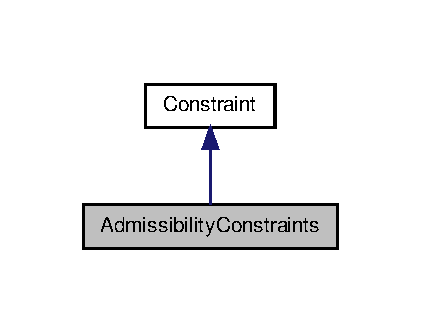
\includegraphics[width=202pt]{classAdmissibilityConstraints__inherit__graph}
\end{center}
\end{figure}


\-Collaboration diagram for \-Admissibility\-Constraints\-:\nopagebreak
\begin{figure}[H]
\begin{center}
\leavevmode
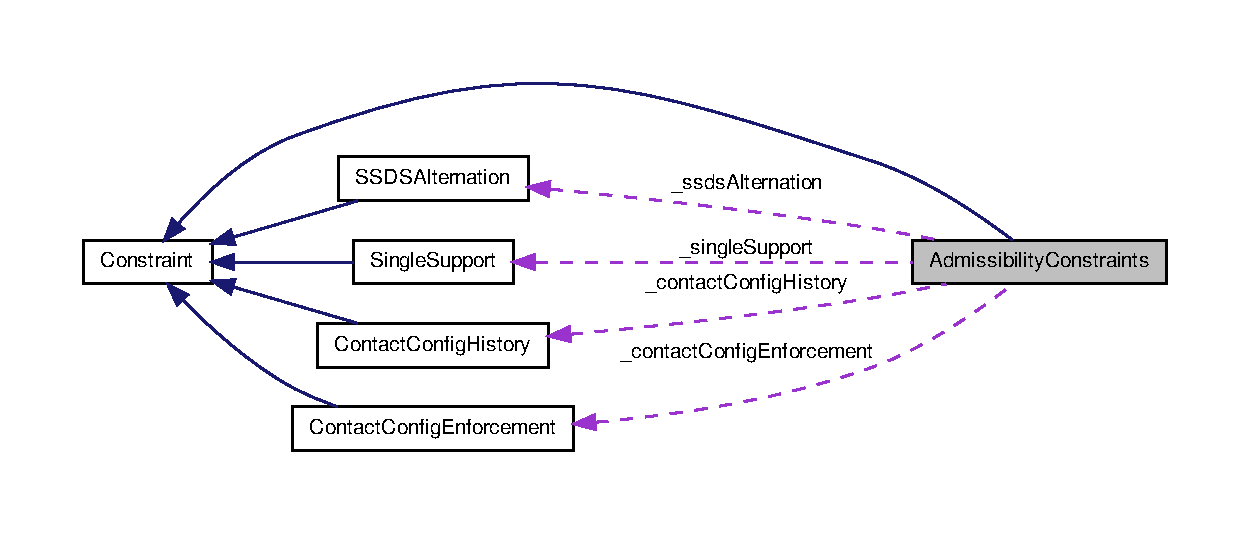
\includegraphics[width=350pt]{classAdmissibilityConstraints__coll__graph}
\end{center}
\end{figure}
\subsection*{\-Public \-Member \-Functions}
\begin{DoxyCompactItemize}
\item 
\hyperlink{classAdmissibilityConstraints_a43220ed86e4b8b841e24e39fc91628a6}{\-Admissibility\-Constraints} ()
\item 
virtual \hyperlink{classAdmissibilityConstraints_a7daa761292772da2f01084584fc46736}{$\sim$\-Admissibility\-Constraints} ()
\end{DoxyCompactItemize}
\subsection*{\-Protected \-Member \-Functions}
\begin{DoxyCompactItemize}
\item 
virtual void \hyperlink{classAdmissibilityConstraints_a22333fbffb9df28433e066b5a00a9c00}{build\-Matrix\-Ci} ()
\item 
virtual void \hyperlink{classAdmissibilityConstraints_a98de6682160b1161d0eb57852ccfce25}{build\-Matrix\-Cii} ()
\item 
virtual void \hyperlink{classAdmissibilityConstraints_a48f89a09f8c9607925652622a8c70fb4}{build\-Vectord} ()
\end{DoxyCompactItemize}
\subsection*{\-Protected \-Attributes}
\begin{DoxyCompactItemize}
\item 
\hyperlink{classSingleSupport}{\-Single\-Support} \hyperlink{classAdmissibilityConstraints_aee4eb816d53a047667da3a7a1f1cac7a}{\-\_\-single\-Support}
\item 
\hyperlink{classSSDSAlternation}{\-S\-S\-D\-S\-Alternation} \hyperlink{classAdmissibilityConstraints_a250631ea82f9c5f88a785537f9e1e9a4}{\-\_\-ssds\-Alternation}
\item 
\hyperlink{classContactConfigHistory}{\-Contact\-Config\-History} \hyperlink{classAdmissibilityConstraints_af2e1d259480686b009077f0c20892bef}{\-\_\-contact\-Config\-History}
\item 
\hyperlink{classContactConfigEnforcement}{\-Contact\-Config\-Enforcement} \hyperlink{classAdmissibilityConstraints_af782db54a141b07c490f726187e2ca8e}{\-\_\-contact\-Config\-Enforcement}
\end{DoxyCompactItemize}


\subsection{\-Constructor \& \-Destructor \-Documentation}
\hypertarget{classAdmissibilityConstraints_a43220ed86e4b8b841e24e39fc91628a6}{\index{\-Admissibility\-Constraints@{\-Admissibility\-Constraints}!\-Admissibility\-Constraints@{\-Admissibility\-Constraints}}
\index{\-Admissibility\-Constraints@{\-Admissibility\-Constraints}!AdmissibilityConstraints@{\-Admissibility\-Constraints}}
\subsubsection[{\-Admissibility\-Constraints}]{\setlength{\rightskip}{0pt plus 5cm}{\bf \-Admissibility\-Constraints\-::\-Admissibility\-Constraints} (
\begin{DoxyParamCaption}
{}
\end{DoxyParamCaption}
)}}\label{classAdmissibilityConstraints_a43220ed86e4b8b841e24e39fc91628a6}
\hypertarget{classAdmissibilityConstraints_a7daa761292772da2f01084584fc46736}{\index{\-Admissibility\-Constraints@{\-Admissibility\-Constraints}!$\sim$\-Admissibility\-Constraints@{$\sim$\-Admissibility\-Constraints}}
\index{$\sim$\-Admissibility\-Constraints@{$\sim$\-Admissibility\-Constraints}!AdmissibilityConstraints@{\-Admissibility\-Constraints}}
\subsubsection[{$\sim$\-Admissibility\-Constraints}]{\setlength{\rightskip}{0pt plus 5cm}{\bf \-Admissibility\-Constraints\-::$\sim$\-Admissibility\-Constraints} (
\begin{DoxyParamCaption}
{}
\end{DoxyParamCaption}
)\hspace{0.3cm}{\ttfamily  \mbox{[}virtual\mbox{]}}}}\label{classAdmissibilityConstraints_a7daa761292772da2f01084584fc46736}


\subsection{\-Member \-Function \-Documentation}
\hypertarget{classAdmissibilityConstraints_a22333fbffb9df28433e066b5a00a9c00}{\index{\-Admissibility\-Constraints@{\-Admissibility\-Constraints}!build\-Matrix\-Ci@{build\-Matrix\-Ci}}
\index{build\-Matrix\-Ci@{build\-Matrix\-Ci}!AdmissibilityConstraints@{\-Admissibility\-Constraints}}
\subsubsection[{build\-Matrix\-Ci}]{\setlength{\rightskip}{0pt plus 5cm}void {\bf \-Admissibility\-Constraints\-::build\-Matrix\-Ci} (
\begin{DoxyParamCaption}
{}
\end{DoxyParamCaption}
)\hspace{0.3cm}{\ttfamily  \mbox{[}protected, virtual\mbox{]}}}}\label{classAdmissibilityConstraints_a22333fbffb9df28433e066b5a00a9c00}


\-Reimplemented from \hyperlink{classConstraint_acc08adc7b34825792cb0127a0d699269}{\-Constraint}.

\hypertarget{classAdmissibilityConstraints_a98de6682160b1161d0eb57852ccfce25}{\index{\-Admissibility\-Constraints@{\-Admissibility\-Constraints}!build\-Matrix\-Cii@{build\-Matrix\-Cii}}
\index{build\-Matrix\-Cii@{build\-Matrix\-Cii}!AdmissibilityConstraints@{\-Admissibility\-Constraints}}
\subsubsection[{build\-Matrix\-Cii}]{\setlength{\rightskip}{0pt plus 5cm}void {\bf \-Admissibility\-Constraints\-::build\-Matrix\-Cii} (
\begin{DoxyParamCaption}
{}
\end{DoxyParamCaption}
)\hspace{0.3cm}{\ttfamily  \mbox{[}protected, virtual\mbox{]}}}}\label{classAdmissibilityConstraints_a98de6682160b1161d0eb57852ccfce25}


\-Reimplemented from \hyperlink{classConstraint_aef7c4d1071c06f34fbc5c0f06105418f}{\-Constraint}.

\hypertarget{classAdmissibilityConstraints_a48f89a09f8c9607925652622a8c70fb4}{\index{\-Admissibility\-Constraints@{\-Admissibility\-Constraints}!build\-Vectord@{build\-Vectord}}
\index{build\-Vectord@{build\-Vectord}!AdmissibilityConstraints@{\-Admissibility\-Constraints}}
\subsubsection[{build\-Vectord}]{\setlength{\rightskip}{0pt plus 5cm}void {\bf \-Admissibility\-Constraints\-::build\-Vectord} (
\begin{DoxyParamCaption}
{}
\end{DoxyParamCaption}
)\hspace{0.3cm}{\ttfamily  \mbox{[}protected, virtual\mbox{]}}}}\label{classAdmissibilityConstraints_a48f89a09f8c9607925652622a8c70fb4}


\-Reimplemented from \hyperlink{classConstraint_a07453509c3f0f95034db965c9e699810}{\-Constraint}.



\subsection{\-Member \-Data \-Documentation}
\hypertarget{classAdmissibilityConstraints_af782db54a141b07c490f726187e2ca8e}{\index{\-Admissibility\-Constraints@{\-Admissibility\-Constraints}!\-\_\-contact\-Config\-Enforcement@{\-\_\-contact\-Config\-Enforcement}}
\index{\-\_\-contact\-Config\-Enforcement@{\-\_\-contact\-Config\-Enforcement}!AdmissibilityConstraints@{\-Admissibility\-Constraints}}
\subsubsection[{\-\_\-contact\-Config\-Enforcement}]{\setlength{\rightskip}{0pt plus 5cm}{\bf \-Contact\-Config\-Enforcement} {\bf \-Admissibility\-Constraints\-::\-\_\-contact\-Config\-Enforcement}\hspace{0.3cm}{\ttfamily  \mbox{[}protected\mbox{]}}}}\label{classAdmissibilityConstraints_af782db54a141b07c490f726187e2ca8e}
\hypertarget{classAdmissibilityConstraints_af2e1d259480686b009077f0c20892bef}{\index{\-Admissibility\-Constraints@{\-Admissibility\-Constraints}!\-\_\-contact\-Config\-History@{\-\_\-contact\-Config\-History}}
\index{\-\_\-contact\-Config\-History@{\-\_\-contact\-Config\-History}!AdmissibilityConstraints@{\-Admissibility\-Constraints}}
\subsubsection[{\-\_\-contact\-Config\-History}]{\setlength{\rightskip}{0pt plus 5cm}{\bf \-Contact\-Config\-History} {\bf \-Admissibility\-Constraints\-::\-\_\-contact\-Config\-History}\hspace{0.3cm}{\ttfamily  \mbox{[}protected\mbox{]}}}}\label{classAdmissibilityConstraints_af2e1d259480686b009077f0c20892bef}
\hypertarget{classAdmissibilityConstraints_aee4eb816d53a047667da3a7a1f1cac7a}{\index{\-Admissibility\-Constraints@{\-Admissibility\-Constraints}!\-\_\-single\-Support@{\-\_\-single\-Support}}
\index{\-\_\-single\-Support@{\-\_\-single\-Support}!AdmissibilityConstraints@{\-Admissibility\-Constraints}}
\subsubsection[{\-\_\-single\-Support}]{\setlength{\rightskip}{0pt plus 5cm}{\bf \-Single\-Support} {\bf \-Admissibility\-Constraints\-::\-\_\-single\-Support}\hspace{0.3cm}{\ttfamily  \mbox{[}protected\mbox{]}}}}\label{classAdmissibilityConstraints_aee4eb816d53a047667da3a7a1f1cac7a}
\hypertarget{classAdmissibilityConstraints_a250631ea82f9c5f88a785537f9e1e9a4}{\index{\-Admissibility\-Constraints@{\-Admissibility\-Constraints}!\-\_\-ssds\-Alternation@{\-\_\-ssds\-Alternation}}
\index{\-\_\-ssds\-Alternation@{\-\_\-ssds\-Alternation}!AdmissibilityConstraints@{\-Admissibility\-Constraints}}
\subsubsection[{\-\_\-ssds\-Alternation}]{\setlength{\rightskip}{0pt plus 5cm}{\bf \-S\-S\-D\-S\-Alternation} {\bf \-Admissibility\-Constraints\-::\-\_\-ssds\-Alternation}\hspace{0.3cm}{\ttfamily  \mbox{[}protected\mbox{]}}}}\label{classAdmissibilityConstraints_a250631ea82f9c5f88a785537f9e1e9a4}


\-The documentation for this class was generated from the following files\-:\begin{DoxyCompactItemize}
\item 
ocra-\/wbi-\/plugins/ocra-\/icub-\/clients/walking-\/client/include/walking-\/client/constraints/\hyperlink{AdmissibilityConstraints_8h}{\-Admissibility\-Constraints.\-h}\item 
ocra-\/wbi-\/plugins/ocra-\/icub-\/clients/walking-\/client/src/\hyperlink{AdmissibilityConstraints_8cpp}{\-Admissibility\-Constraints.\-cpp}\end{DoxyCompactItemize}

\hypertarget{structAdmissibilityConstraintsStruct}{\section{\-Admissibility\-Constraints\-Struct \-Struct \-Reference}
\label{structAdmissibilityConstraintsStruct}\index{\-Admissibility\-Constraints\-Struct@{\-Admissibility\-Constraints\-Struct}}
}


{\ttfamily \#include $<$constraints\-Structs.\-h$>$}



\-Collaboration diagram for \-Admissibility\-Constraints\-Struct\-:\nopagebreak
\begin{figure}[H]
\begin{center}
\leavevmode
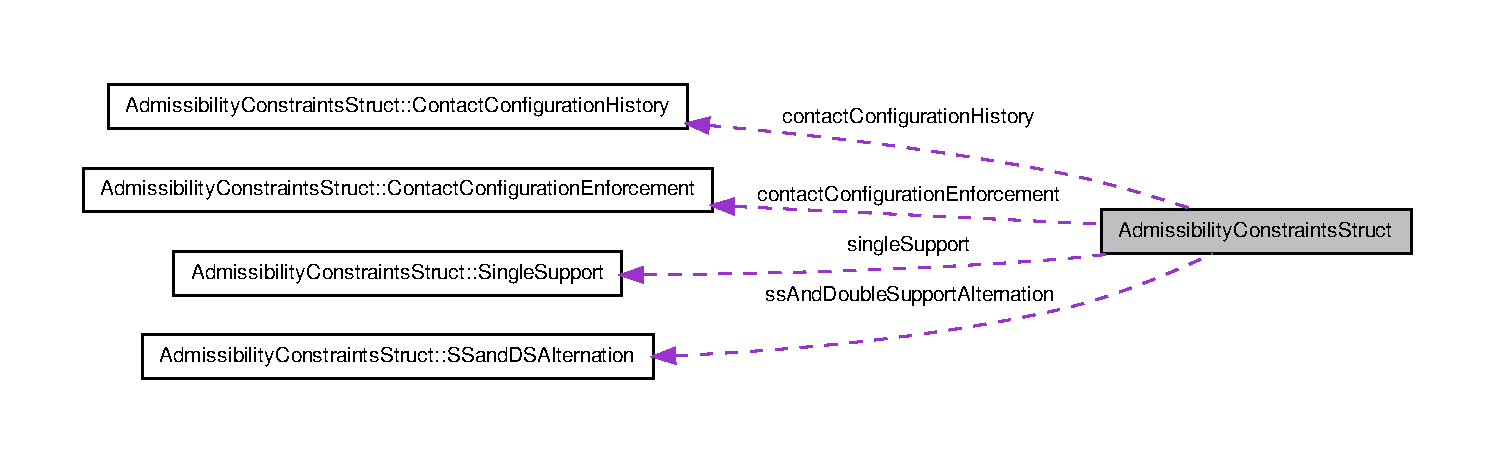
\includegraphics[width=350pt]{structAdmissibilityConstraintsStruct__coll__graph}
\end{center}
\end{figure}
\subsection*{\-Classes}
\begin{DoxyCompactItemize}
\item 
struct \hyperlink{structAdmissibilityConstraintsStruct_1_1ContactConfigurationEnforcement}{\-Contact\-Configuration\-Enforcement}
\item 
struct \hyperlink{structAdmissibilityConstraintsStruct_1_1ContactConfigurationHistory}{\-Contact\-Configuration\-History}
\item 
struct \hyperlink{structAdmissibilityConstraintsStruct_1_1SingleSupport}{\-Single\-Support}
\item 
struct \hyperlink{structAdmissibilityConstraintsStruct_1_1SSandDSAlternation}{\-S\-Sand\-D\-S\-Alternation}
\end{DoxyCompactItemize}
\subsection*{\-Public \-Attributes}
\begin{DoxyCompactItemize}
\item 
\-Eigen\-::\-Matrix\-Xd \hyperlink{structAdmissibilityConstraintsStruct_a98a5ca7c248a90da7503646cc79476e3}{\-Cbar}
\item 
\-Eigen\-::\-Vector\-Xd \hyperlink{structAdmissibilityConstraintsStruct_a9db3c58cd73ef8ef0bb74f71ae9bb225}{dbar}
\item 
\-Eigen\-::\-Vector\-Xd \hyperlink{structAdmissibilityConstraintsStruct_adadbcf470bb052caccee15b81000684a}{f\-History}
\item 
\hyperlink{structAdmissibilityConstraintsStruct_1_1SSandDSAlternation}{\-S\-Sand\-D\-S\-Alternation} \hyperlink{structAdmissibilityConstraintsStruct_a387b2106272e3148e1fd4dbde6dedb3e}{ss\-And\-Double\-Support\-Alternation}
\item 
\hyperlink{structAdmissibilityConstraintsStruct_1_1SingleSupport}{\-Single\-Support} \hyperlink{structAdmissibilityConstraintsStruct_a40fb404909b4fcee9e31e1dbf566a554}{single\-Support}
\item 
\hyperlink{structAdmissibilityConstraintsStruct_1_1ContactConfigurationHistory}{\-Contact\-Configuration\-History} \hyperlink{structAdmissibilityConstraintsStruct_a1869779fd2f2d7a1a3d352ddb783052d}{contact\-Configuration\-History}
\item 
\hyperlink{structAdmissibilityConstraintsStruct_1_1ContactConfigurationEnforcement}{\-Contact\-Configuration\-Enforcement} \hyperlink{structAdmissibilityConstraintsStruct_af002ab19787c812e98ed8fbff1f1cae5}{contact\-Configuration\-Enforcement}
\end{DoxyCompactItemize}


\subsection{\-Member \-Data \-Documentation}
\hypertarget{structAdmissibilityConstraintsStruct_a98a5ca7c248a90da7503646cc79476e3}{\index{\-Admissibility\-Constraints\-Struct@{\-Admissibility\-Constraints\-Struct}!\-Cbar@{\-Cbar}}
\index{\-Cbar@{\-Cbar}!AdmissibilityConstraintsStruct@{\-Admissibility\-Constraints\-Struct}}
\subsubsection[{\-Cbar}]{\setlength{\rightskip}{0pt plus 5cm}\-Eigen\-::\-Matrix\-Xd {\bf \-Admissibility\-Constraints\-Struct\-::\-Cbar}}}\label{structAdmissibilityConstraintsStruct_a98a5ca7c248a90da7503646cc79476e3}
\hypertarget{structAdmissibilityConstraintsStruct_af002ab19787c812e98ed8fbff1f1cae5}{\index{\-Admissibility\-Constraints\-Struct@{\-Admissibility\-Constraints\-Struct}!contact\-Configuration\-Enforcement@{contact\-Configuration\-Enforcement}}
\index{contact\-Configuration\-Enforcement@{contact\-Configuration\-Enforcement}!AdmissibilityConstraintsStruct@{\-Admissibility\-Constraints\-Struct}}
\subsubsection[{contact\-Configuration\-Enforcement}]{\setlength{\rightskip}{0pt plus 5cm}{\bf \-Contact\-Configuration\-Enforcement} {\bf \-Admissibility\-Constraints\-Struct\-::contact\-Configuration\-Enforcement}}}\label{structAdmissibilityConstraintsStruct_af002ab19787c812e98ed8fbff1f1cae5}
\hypertarget{structAdmissibilityConstraintsStruct_a1869779fd2f2d7a1a3d352ddb783052d}{\index{\-Admissibility\-Constraints\-Struct@{\-Admissibility\-Constraints\-Struct}!contact\-Configuration\-History@{contact\-Configuration\-History}}
\index{contact\-Configuration\-History@{contact\-Configuration\-History}!AdmissibilityConstraintsStruct@{\-Admissibility\-Constraints\-Struct}}
\subsubsection[{contact\-Configuration\-History}]{\setlength{\rightskip}{0pt plus 5cm}{\bf \-Contact\-Configuration\-History} {\bf \-Admissibility\-Constraints\-Struct\-::contact\-Configuration\-History}}}\label{structAdmissibilityConstraintsStruct_a1869779fd2f2d7a1a3d352ddb783052d}
\hypertarget{structAdmissibilityConstraintsStruct_a9db3c58cd73ef8ef0bb74f71ae9bb225}{\index{\-Admissibility\-Constraints\-Struct@{\-Admissibility\-Constraints\-Struct}!dbar@{dbar}}
\index{dbar@{dbar}!AdmissibilityConstraintsStruct@{\-Admissibility\-Constraints\-Struct}}
\subsubsection[{dbar}]{\setlength{\rightskip}{0pt plus 5cm}\-Eigen\-::\-Vector\-Xd {\bf \-Admissibility\-Constraints\-Struct\-::dbar}}}\label{structAdmissibilityConstraintsStruct_a9db3c58cd73ef8ef0bb74f71ae9bb225}
\hypertarget{structAdmissibilityConstraintsStruct_adadbcf470bb052caccee15b81000684a}{\index{\-Admissibility\-Constraints\-Struct@{\-Admissibility\-Constraints\-Struct}!f\-History@{f\-History}}
\index{f\-History@{f\-History}!AdmissibilityConstraintsStruct@{\-Admissibility\-Constraints\-Struct}}
\subsubsection[{f\-History}]{\setlength{\rightskip}{0pt plus 5cm}\-Eigen\-::\-Vector\-Xd {\bf \-Admissibility\-Constraints\-Struct\-::f\-History}}}\label{structAdmissibilityConstraintsStruct_adadbcf470bb052caccee15b81000684a}
\hypertarget{structAdmissibilityConstraintsStruct_a40fb404909b4fcee9e31e1dbf566a554}{\index{\-Admissibility\-Constraints\-Struct@{\-Admissibility\-Constraints\-Struct}!single\-Support@{single\-Support}}
\index{single\-Support@{single\-Support}!AdmissibilityConstraintsStruct@{\-Admissibility\-Constraints\-Struct}}
\subsubsection[{single\-Support}]{\setlength{\rightskip}{0pt plus 5cm}{\bf \-Single\-Support} {\bf \-Admissibility\-Constraints\-Struct\-::single\-Support}}}\label{structAdmissibilityConstraintsStruct_a40fb404909b4fcee9e31e1dbf566a554}
\hypertarget{structAdmissibilityConstraintsStruct_a387b2106272e3148e1fd4dbde6dedb3e}{\index{\-Admissibility\-Constraints\-Struct@{\-Admissibility\-Constraints\-Struct}!ss\-And\-Double\-Support\-Alternation@{ss\-And\-Double\-Support\-Alternation}}
\index{ss\-And\-Double\-Support\-Alternation@{ss\-And\-Double\-Support\-Alternation}!AdmissibilityConstraintsStruct@{\-Admissibility\-Constraints\-Struct}}
\subsubsection[{ss\-And\-Double\-Support\-Alternation}]{\setlength{\rightskip}{0pt plus 5cm}{\bf \-S\-Sand\-D\-S\-Alternation} {\bf \-Admissibility\-Constraints\-Struct\-::ss\-And\-Double\-Support\-Alternation}}}\label{structAdmissibilityConstraintsStruct_a387b2106272e3148e1fd4dbde6dedb3e}


\-The documentation for this struct was generated from the following file\-:\begin{DoxyCompactItemize}
\item 
ocra-\/wbi-\/plugins/ocra-\/icub-\/clients/walking-\/client/include/walking-\/client/\hyperlink{constraintsStructs_8h}{constraints\-Structs.\-h}\end{DoxyCompactItemize}

\hypertarget{classBaseOfSupport}{\section{\-Base\-Of\-Support \-Class \-Reference}
\label{classBaseOfSupport}\index{\-Base\-Of\-Support@{\-Base\-Of\-Support}}
}


\-Builds base of support and corresponding constraints based on the robot's feet location.  




{\ttfamily \#include $<$\-Base\-Of\-Support.\-h$>$}

\subsection*{\-Public \-Member \-Functions}
\begin{DoxyCompactItemize}
\item 
\hyperlink{classBaseOfSupport_a2490d7d641608be3b85c903de83313cc}{\-Base\-Of\-Support} (std\-::shared\-\_\-ptr$<$ \hyperlink{classStepController}{\-Step\-Controller} $>$ step\-Controller)
\item 
virtual \hyperlink{classBaseOfSupport_a8f2261d4d25cd677d0114df426dfbfa7}{$\sim$\-Base\-Of\-Support} ()
\item 
void \hyperlink{classBaseOfSupport_af88e70d87098060a46e4a6fc9c876a22}{compute\-Bo\-S\-Center} (\-Eigen\-::\-Vector2d \&r)
\item 
void \hyperlink{classBaseOfSupport_ac0e7a364ac0ac945469a34d12ab3c9f4}{compute\-Aand\-B} (\-Eigen\-::\-Matrix\-Xd \&list\-Convex\-Hull, \-Eigen\-::\-Vector2d a, \-Eigen\-::\-Vector2d b)
\item 
void \hyperlink{classBaseOfSupport_a09b197a9869db126658d227532c1e03a}{compute\-Ai\-Bi} (\-Eigen\-::\-Vector2d r, \-Eigen\-::\-Vector2d p1, \-Eigen\-::\-Vector2d p2, \-Eigen\-::\-Row\-Vector2d \&\-Ai, double \&bi, double tol\-Diff=1e-\/2)
\item 
void \hyperlink{classBaseOfSupport_ad9a709f6df002662bfd67982a2c0e201}{compute\-Midpoint} (\-Eigen\-::\-Vector2d a, \-Eigen\-::\-Vector2d b, \-Eigen\-::\-Vector2d \&r)
\item 
bool \hyperlink{classBaseOfSupport_af7907a87712c10c72f812f0304c013e4}{update} (\-Eigen\-::\-Vector\-Xd xi\-\_\-k)
\item 
\-Eigen\-::\-Matrix\-Xd \hyperlink{classBaseOfSupport_ae98c5398e4c53666e324c1fcfb1ef167}{compute\-Convex\-Hull} (\-Eigen\-::\-Matrix\-Xd \&feet\-Corners)
\item 
\-Eigen\-::\-Matrix\-Xd \hyperlink{classBaseOfSupport_afc033ba8e5530f667f90ae539adb27f3}{get\-Feet\-Corners} (int gamma)
\end{DoxyCompactItemize}
\subsection*{\-Private \-Attributes}
\begin{DoxyCompactItemize}
\item 
\-Eigen\-::\-Matrix\-Xd \hyperlink{classBaseOfSupport_a54a35d087a8dfaee9a27d025d46f706d}{\-\_\-\-A}
\item 
\-Eigen\-::\-Vector\-Xd \hyperlink{classBaseOfSupport_adfa70199064a50d9d7aea9a6d4b13246}{\-\_\-\-B}
\item 
\hyperlink{BaseOfSupport_8h_a3b0bf53b9d321e300a59729ebe10e02c}{\-Polygon} \hyperlink{classBaseOfSupport_a7e9b4ef515f90e2a7012871e7287bf5e}{\-\_\-poly}
\item 
\hyperlink{BaseOfSupport_8h_a3b0bf53b9d321e300a59729ebe10e02c}{\-Polygon} \hyperlink{classBaseOfSupport_a3caa9bcea814865f12d891c0a1c8c4ea}{\-\_\-hull}
\item 
std\-::shared\-\_\-ptr$<$ \hyperlink{classStepController}{\-Step\-Controller} $>$ \hyperlink{classBaseOfSupport_a023d28c6900f0e97d9de42ca2c5d94a5}{\-\_\-step\-Controller}
\end{DoxyCompactItemize}


\subsection{\-Detailed \-Description}
\-Builds base of support and corresponding constraints based on the robot's feet location. 

\begin{DoxyAuthor}{\-Author}
\-Jorhabib \-Eljaik \cite{ibanezThesis2015} 
\end{DoxyAuthor}
\begin{DoxyWarning}{\-Warning}
\-Work in progress! \-This is still a barebone class in the process of being tested.
\end{DoxyWarning}
\-This class uses the \-Geometry \-Boost libraries in order to find the vertices of the base of support (support polygon) defined by the location of the feet of the robot. \-Afterwards, it will build the inequality constraints that define the area of this polygon, useful to \hyperlink{classMIQPLinearConstraints}{\-M\-I\-Q\-P\-Linear\-Constraints} to define the constraints on the \-Center of \-Pressure which should always lie within the support polygon. 

\subsection{\-Constructor \& \-Destructor \-Documentation}
\hypertarget{classBaseOfSupport_a2490d7d641608be3b85c903de83313cc}{\index{\-Base\-Of\-Support@{\-Base\-Of\-Support}!\-Base\-Of\-Support@{\-Base\-Of\-Support}}
\index{\-Base\-Of\-Support@{\-Base\-Of\-Support}!BaseOfSupport@{\-Base\-Of\-Support}}
\subsubsection[{\-Base\-Of\-Support}]{\setlength{\rightskip}{0pt plus 5cm}{\bf \-Base\-Of\-Support\-::\-Base\-Of\-Support} (
\begin{DoxyParamCaption}
\item[{std\-::shared\-\_\-ptr$<$ {\bf \-Step\-Controller} $>$}]{step\-Controller}
\end{DoxyParamCaption}
)}}\label{classBaseOfSupport_a2490d7d641608be3b85c903de83313cc}
\hypertarget{classBaseOfSupport_a8f2261d4d25cd677d0114df426dfbfa7}{\index{\-Base\-Of\-Support@{\-Base\-Of\-Support}!$\sim$\-Base\-Of\-Support@{$\sim$\-Base\-Of\-Support}}
\index{$\sim$\-Base\-Of\-Support@{$\sim$\-Base\-Of\-Support}!BaseOfSupport@{\-Base\-Of\-Support}}
\subsubsection[{$\sim$\-Base\-Of\-Support}]{\setlength{\rightskip}{0pt plus 5cm}{\bf \-Base\-Of\-Support\-::$\sim$\-Base\-Of\-Support} (
\begin{DoxyParamCaption}
{}
\end{DoxyParamCaption}
)\hspace{0.3cm}{\ttfamily  \mbox{[}virtual\mbox{]}}}}\label{classBaseOfSupport_a8f2261d4d25cd677d0114df426dfbfa7}


\subsection{\-Member \-Function \-Documentation}
\hypertarget{classBaseOfSupport_ac0e7a364ac0ac945469a34d12ab3c9f4}{\index{\-Base\-Of\-Support@{\-Base\-Of\-Support}!compute\-Aand\-B@{compute\-Aand\-B}}
\index{compute\-Aand\-B@{compute\-Aand\-B}!BaseOfSupport@{\-Base\-Of\-Support}}
\subsubsection[{compute\-Aand\-B}]{\setlength{\rightskip}{0pt plus 5cm}void {\bf \-Base\-Of\-Support\-::compute\-Aand\-B} (
\begin{DoxyParamCaption}
\item[{\-Eigen\-::\-Matrix\-Xd \&}]{list\-Convex\-Hull, }
\item[{\-Eigen\-::\-Vector2d}]{a, }
\item[{\-Eigen\-::\-Vector2d}]{b}
\end{DoxyParamCaption}
)}}\label{classBaseOfSupport_ac0e7a364ac0ac945469a34d12ab3c9f4}
\hypertarget{classBaseOfSupport_a09b197a9869db126658d227532c1e03a}{\index{\-Base\-Of\-Support@{\-Base\-Of\-Support}!compute\-Ai\-Bi@{compute\-Ai\-Bi}}
\index{compute\-Ai\-Bi@{compute\-Ai\-Bi}!BaseOfSupport@{\-Base\-Of\-Support}}
\subsubsection[{compute\-Ai\-Bi}]{\setlength{\rightskip}{0pt plus 5cm}void {\bf \-Base\-Of\-Support\-::compute\-Ai\-Bi} (
\begin{DoxyParamCaption}
\item[{\-Eigen\-::\-Vector2d}]{r, }
\item[{\-Eigen\-::\-Vector2d}]{p1, }
\item[{\-Eigen\-::\-Vector2d}]{p2, }
\item[{\-Eigen\-::\-Row\-Vector2d \&}]{\-Ai, }
\item[{double \&}]{bi, }
\item[{double}]{tol\-Diff = {\ttfamily 1e-\/2}}
\end{DoxyParamCaption}
)}}\label{classBaseOfSupport_a09b197a9869db126658d227532c1e03a}
\hypertarget{classBaseOfSupport_af88e70d87098060a46e4a6fc9c876a22}{\index{\-Base\-Of\-Support@{\-Base\-Of\-Support}!compute\-Bo\-S\-Center@{compute\-Bo\-S\-Center}}
\index{compute\-Bo\-S\-Center@{compute\-Bo\-S\-Center}!BaseOfSupport@{\-Base\-Of\-Support}}
\subsubsection[{compute\-Bo\-S\-Center}]{\setlength{\rightskip}{0pt plus 5cm}void {\bf \-Base\-Of\-Support\-::compute\-Bo\-S\-Center} (
\begin{DoxyParamCaption}
\item[{\-Eigen\-::\-Vector2d \&}]{r}
\end{DoxyParamCaption}
)}}\label{classBaseOfSupport_af88e70d87098060a46e4a6fc9c876a22}
\hypertarget{classBaseOfSupport_ae98c5398e4c53666e324c1fcfb1ef167}{\index{\-Base\-Of\-Support@{\-Base\-Of\-Support}!compute\-Convex\-Hull@{compute\-Convex\-Hull}}
\index{compute\-Convex\-Hull@{compute\-Convex\-Hull}!BaseOfSupport@{\-Base\-Of\-Support}}
\subsubsection[{compute\-Convex\-Hull}]{\setlength{\rightskip}{0pt plus 5cm}\-Eigen\-::\-Matrix\-Xd {\bf \-Base\-Of\-Support\-::compute\-Convex\-Hull} (
\begin{DoxyParamCaption}
\item[{\-Eigen\-::\-Matrix\-Xd \&}]{feet\-Corners}
\end{DoxyParamCaption}
)}}\label{classBaseOfSupport_ae98c5398e4c53666e324c1fcfb1ef167}
\hypertarget{classBaseOfSupport_ad9a709f6df002662bfd67982a2c0e201}{\index{\-Base\-Of\-Support@{\-Base\-Of\-Support}!compute\-Midpoint@{compute\-Midpoint}}
\index{compute\-Midpoint@{compute\-Midpoint}!BaseOfSupport@{\-Base\-Of\-Support}}
\subsubsection[{compute\-Midpoint}]{\setlength{\rightskip}{0pt plus 5cm}void {\bf \-Base\-Of\-Support\-::compute\-Midpoint} (
\begin{DoxyParamCaption}
\item[{\-Eigen\-::\-Vector2d}]{a, }
\item[{\-Eigen\-::\-Vector2d}]{b, }
\item[{\-Eigen\-::\-Vector2d \&}]{r}
\end{DoxyParamCaption}
)}}\label{classBaseOfSupport_ad9a709f6df002662bfd67982a2c0e201}
\hypertarget{classBaseOfSupport_afc033ba8e5530f667f90ae539adb27f3}{\index{\-Base\-Of\-Support@{\-Base\-Of\-Support}!get\-Feet\-Corners@{get\-Feet\-Corners}}
\index{get\-Feet\-Corners@{get\-Feet\-Corners}!BaseOfSupport@{\-Base\-Of\-Support}}
\subsubsection[{get\-Feet\-Corners}]{\setlength{\rightskip}{0pt plus 5cm}\-Eigen\-::\-Matrix\-Xd {\bf \-Base\-Of\-Support\-::get\-Feet\-Corners} (
\begin{DoxyParamCaption}
\item[{int}]{gamma}
\end{DoxyParamCaption}
)}}\label{classBaseOfSupport_afc033ba8e5530f667f90ae539adb27f3}
\hypertarget{classBaseOfSupport_af7907a87712c10c72f812f0304c013e4}{\index{\-Base\-Of\-Support@{\-Base\-Of\-Support}!update@{update}}
\index{update@{update}!BaseOfSupport@{\-Base\-Of\-Support}}
\subsubsection[{update}]{\setlength{\rightskip}{0pt plus 5cm}bool {\bf \-Base\-Of\-Support\-::update} (
\begin{DoxyParamCaption}
\item[{\-Eigen\-::\-Vector\-Xd}]{xi\-\_\-k}
\end{DoxyParamCaption}
)}}\label{classBaseOfSupport_af7907a87712c10c72f812f0304c013e4}


\subsection{\-Member \-Data \-Documentation}
\hypertarget{classBaseOfSupport_a54a35d087a8dfaee9a27d025d46f706d}{\index{\-Base\-Of\-Support@{\-Base\-Of\-Support}!\-\_\-\-A@{\-\_\-\-A}}
\index{\-\_\-\-A@{\-\_\-\-A}!BaseOfSupport@{\-Base\-Of\-Support}}
\subsubsection[{\-\_\-\-A}]{\setlength{\rightskip}{0pt plus 5cm}\-Eigen\-::\-Matrix\-Xd {\bf \-Base\-Of\-Support\-::\-\_\-\-A}\hspace{0.3cm}{\ttfamily  \mbox{[}private\mbox{]}}}}\label{classBaseOfSupport_a54a35d087a8dfaee9a27d025d46f706d}
\hypertarget{classBaseOfSupport_adfa70199064a50d9d7aea9a6d4b13246}{\index{\-Base\-Of\-Support@{\-Base\-Of\-Support}!\-\_\-\-B@{\-\_\-\-B}}
\index{\-\_\-\-B@{\-\_\-\-B}!BaseOfSupport@{\-Base\-Of\-Support}}
\subsubsection[{\-\_\-\-B}]{\setlength{\rightskip}{0pt plus 5cm}\-Eigen\-::\-Vector\-Xd {\bf \-Base\-Of\-Support\-::\-\_\-\-B}\hspace{0.3cm}{\ttfamily  \mbox{[}private\mbox{]}}}}\label{classBaseOfSupport_adfa70199064a50d9d7aea9a6d4b13246}
\hypertarget{classBaseOfSupport_a3caa9bcea814865f12d891c0a1c8c4ea}{\index{\-Base\-Of\-Support@{\-Base\-Of\-Support}!\-\_\-hull@{\-\_\-hull}}
\index{\-\_\-hull@{\-\_\-hull}!BaseOfSupport@{\-Base\-Of\-Support}}
\subsubsection[{\-\_\-hull}]{\setlength{\rightskip}{0pt plus 5cm}{\bf \-Polygon} {\bf \-Base\-Of\-Support\-::\-\_\-hull}\hspace{0.3cm}{\ttfamily  \mbox{[}private\mbox{]}}}}\label{classBaseOfSupport_a3caa9bcea814865f12d891c0a1c8c4ea}
\hypertarget{classBaseOfSupport_a7e9b4ef515f90e2a7012871e7287bf5e}{\index{\-Base\-Of\-Support@{\-Base\-Of\-Support}!\-\_\-poly@{\-\_\-poly}}
\index{\-\_\-poly@{\-\_\-poly}!BaseOfSupport@{\-Base\-Of\-Support}}
\subsubsection[{\-\_\-poly}]{\setlength{\rightskip}{0pt plus 5cm}{\bf \-Polygon} {\bf \-Base\-Of\-Support\-::\-\_\-poly}\hspace{0.3cm}{\ttfamily  \mbox{[}private\mbox{]}}}}\label{classBaseOfSupport_a7e9b4ef515f90e2a7012871e7287bf5e}
\hypertarget{classBaseOfSupport_a023d28c6900f0e97d9de42ca2c5d94a5}{\index{\-Base\-Of\-Support@{\-Base\-Of\-Support}!\-\_\-step\-Controller@{\-\_\-step\-Controller}}
\index{\-\_\-step\-Controller@{\-\_\-step\-Controller}!BaseOfSupport@{\-Base\-Of\-Support}}
\subsubsection[{\-\_\-step\-Controller}]{\setlength{\rightskip}{0pt plus 5cm}std\-::shared\-\_\-ptr$<${\bf \-Step\-Controller}$>$ {\bf \-Base\-Of\-Support\-::\-\_\-step\-Controller}\hspace{0.3cm}{\ttfamily  \mbox{[}private\mbox{]}}}}\label{classBaseOfSupport_a023d28c6900f0e97d9de42ca2c5d94a5}


\-The documentation for this class was generated from the following files\-:\begin{DoxyCompactItemize}
\item 
ocra-\/wbi-\/plugins/ocra-\/icub-\/clients/walking-\/client/include/walking-\/client/\hyperlink{BaseOfSupport_8h}{\-Base\-Of\-Support.\-h}\item 
ocra-\/wbi-\/plugins/ocra-\/icub-\/clients/walking-\/client/src/\hyperlink{BaseOfSupport_8cpp}{\-Base\-Of\-Support.\-cpp}\end{DoxyCompactItemize}

\hypertarget{classBounding}{\section{\-Bounding \-Class \-Reference}
\label{classBounding}\index{\-Bounding@{\-Bounding}}
}


{\ttfamily \#include $<$\-Bounding.\-h$>$}



\-Inheritance diagram for \-Bounding\-:
\nopagebreak
\begin{figure}[H]
\begin{center}
\leavevmode
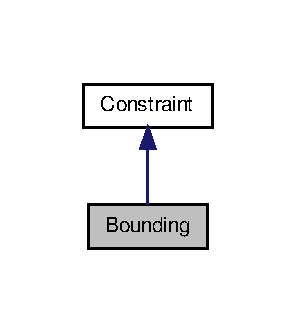
\includegraphics[width=142pt]{classBounding__inherit__graph}
\end{center}
\end{figure}


\-Collaboration diagram for \-Bounding\-:
\nopagebreak
\begin{figure}[H]
\begin{center}
\leavevmode
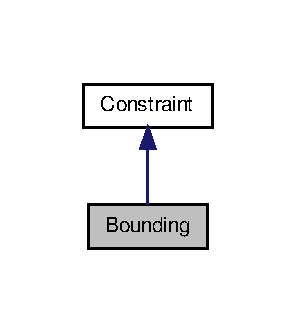
\includegraphics[width=142pt]{classBounding__coll__graph}
\end{center}
\end{figure}
\subsection*{\-Public \-Member \-Functions}
\begin{DoxyCompactItemize}
\item 
\hyperlink{classBounding_ab8478542374a91a79e47ef8bea4c3fca}{\-Bounding} ()
\item 
virtual \hyperlink{classBounding_a8e3b81ea2078454840fe93a44f634d56}{$\sim$\-Bounding} ()
\end{DoxyCompactItemize}
\subsection*{\-Protected \-Member \-Functions}
\begin{DoxyCompactItemize}
\item 
void \hyperlink{classBounding_a3997be7d9301b6e353daf574ce307462}{build\-Matrix\-Ci} ()
\item 
void \hyperlink{classBounding_a885a21bf71462c1c4bbb200d4266ca94}{build\-Matrix\-Cii} ()
\item 
void \hyperlink{classBounding_a2d1a349549b5b0633fb7a5c338cb5cf6}{build\-Vectord} ()
\end{DoxyCompactItemize}


\subsection{\-Constructor \& \-Destructor \-Documentation}
\hypertarget{classBounding_ab8478542374a91a79e47ef8bea4c3fca}{\index{\-Bounding@{\-Bounding}!\-Bounding@{\-Bounding}}
\index{\-Bounding@{\-Bounding}!Bounding@{\-Bounding}}
\subsubsection[{\-Bounding}]{\setlength{\rightskip}{0pt plus 5cm}{\bf \-Bounding\-::\-Bounding} (
\begin{DoxyParamCaption}
{}
\end{DoxyParamCaption}
)}}\label{classBounding_ab8478542374a91a79e47ef8bea4c3fca}
\hypertarget{classBounding_a8e3b81ea2078454840fe93a44f634d56}{\index{\-Bounding@{\-Bounding}!$\sim$\-Bounding@{$\sim$\-Bounding}}
\index{$\sim$\-Bounding@{$\sim$\-Bounding}!Bounding@{\-Bounding}}
\subsubsection[{$\sim$\-Bounding}]{\setlength{\rightskip}{0pt plus 5cm}{\bf \-Bounding\-::$\sim$\-Bounding} (
\begin{DoxyParamCaption}
{}
\end{DoxyParamCaption}
)\hspace{0.3cm}{\ttfamily  \mbox{[}virtual\mbox{]}}}}\label{classBounding_a8e3b81ea2078454840fe93a44f634d56}


\subsection{\-Member \-Function \-Documentation}
\hypertarget{classBounding_a3997be7d9301b6e353daf574ce307462}{\index{\-Bounding@{\-Bounding}!build\-Matrix\-Ci@{build\-Matrix\-Ci}}
\index{build\-Matrix\-Ci@{build\-Matrix\-Ci}!Bounding@{\-Bounding}}
\subsubsection[{build\-Matrix\-Ci}]{\setlength{\rightskip}{0pt plus 5cm}void {\bf \-Bounding\-::build\-Matrix\-Ci} (
\begin{DoxyParamCaption}
{}
\end{DoxyParamCaption}
)\hspace{0.3cm}{\ttfamily  \mbox{[}protected, virtual\mbox{]}}}}\label{classBounding_a3997be7d9301b6e353daf574ce307462}


\-Reimplemented from \hyperlink{classConstraint_acc08adc7b34825792cb0127a0d699269}{\-Constraint}.

\hypertarget{classBounding_a885a21bf71462c1c4bbb200d4266ca94}{\index{\-Bounding@{\-Bounding}!build\-Matrix\-Cii@{build\-Matrix\-Cii}}
\index{build\-Matrix\-Cii@{build\-Matrix\-Cii}!Bounding@{\-Bounding}}
\subsubsection[{build\-Matrix\-Cii}]{\setlength{\rightskip}{0pt plus 5cm}void {\bf \-Bounding\-::build\-Matrix\-Cii} (
\begin{DoxyParamCaption}
{}
\end{DoxyParamCaption}
)\hspace{0.3cm}{\ttfamily  \mbox{[}protected, virtual\mbox{]}}}}\label{classBounding_a885a21bf71462c1c4bbb200d4266ca94}


\-Reimplemented from \hyperlink{classConstraint_aef7c4d1071c06f34fbc5c0f06105418f}{\-Constraint}.

\hypertarget{classBounding_a2d1a349549b5b0633fb7a5c338cb5cf6}{\index{\-Bounding@{\-Bounding}!build\-Vectord@{build\-Vectord}}
\index{build\-Vectord@{build\-Vectord}!Bounding@{\-Bounding}}
\subsubsection[{build\-Vectord}]{\setlength{\rightskip}{0pt plus 5cm}void {\bf \-Bounding\-::build\-Vectord} (
\begin{DoxyParamCaption}
{}
\end{DoxyParamCaption}
)\hspace{0.3cm}{\ttfamily  \mbox{[}protected, virtual\mbox{]}}}}\label{classBounding_a2d1a349549b5b0633fb7a5c338cb5cf6}


\-Reimplemented from \hyperlink{classConstraint_a07453509c3f0f95034db965c9e699810}{\-Constraint}.



\-The documentation for this class was generated from the following files\-:\begin{DoxyCompactItemize}
\item 
ocra-\/wbi-\/plugins/ocra-\/icub-\/clients/walking-\/client/include/walking-\/client/constraints/\hyperlink{Bounding_8h}{\-Bounding.\-h}\item 
ocra-\/wbi-\/plugins/ocra-\/icub-\/clients/walking-\/client/src/\hyperlink{Bounding_8cpp}{\-Bounding.\-cpp}\end{DoxyCompactItemize}

\hypertarget{structShapeConstraintsStruct_1_1boundingStruct}{\section{\-Shape\-Constraints\-Struct\-:\-:bounding\-Struct \-Struct \-Reference}
\label{structShapeConstraintsStruct_1_1boundingStruct}\index{\-Shape\-Constraints\-Struct\-::bounding\-Struct@{\-Shape\-Constraints\-Struct\-::bounding\-Struct}}
}


{\ttfamily \#include $<$constraints\-Structs.\-h$>$}

\subsection*{\-Public \-Attributes}
\begin{DoxyCompactItemize}
\item 
\-Eigen\-::\-Matrix\-Xd \hyperlink{structShapeConstraintsStruct_1_1boundingStruct_a888204a5f7e2ea854715605e1b6ba475}{\-C}
\item 
\-Eigen\-::\-Vector\-Xd \hyperlink{structShapeConstraintsStruct_1_1boundingStruct_a6d157c6e92332f3abdce6ccd12206380}{d}
\item 
\-Eigen\-::\-Matrix\-Xd \hyperlink{structShapeConstraintsStruct_1_1boundingStruct_acc45534da5c8b80be0012f6722d5569f}{\-Cbar}
\item 
\-Eigen\-::\-Vector\-Xd \hyperlink{structShapeConstraintsStruct_1_1boundingStruct_ab7b66b74697f335127d4a8cea0fecc2a}{dbar}
\item 
\-Eigen\-::\-Vector\-Xd \hyperlink{structShapeConstraintsStruct_1_1boundingStruct_aad4aa0527751939d9d1eb75c1f50b41b}{fhistory}
\end{DoxyCompactItemize}


\subsection{\-Member \-Data \-Documentation}
\hypertarget{structShapeConstraintsStruct_1_1boundingStruct_a888204a5f7e2ea854715605e1b6ba475}{\index{\-Shape\-Constraints\-Struct\-::bounding\-Struct@{\-Shape\-Constraints\-Struct\-::bounding\-Struct}!\-C@{\-C}}
\index{\-C@{\-C}!ShapeConstraintsStruct::boundingStruct@{\-Shape\-Constraints\-Struct\-::bounding\-Struct}}
\subsubsection[{\-C}]{\setlength{\rightskip}{0pt plus 5cm}\-Eigen\-::\-Matrix\-Xd {\bf \-Shape\-Constraints\-Struct\-::bounding\-Struct\-::\-C}}}\label{structShapeConstraintsStruct_1_1boundingStruct_a888204a5f7e2ea854715605e1b6ba475}
\hypertarget{structShapeConstraintsStruct_1_1boundingStruct_acc45534da5c8b80be0012f6722d5569f}{\index{\-Shape\-Constraints\-Struct\-::bounding\-Struct@{\-Shape\-Constraints\-Struct\-::bounding\-Struct}!\-Cbar@{\-Cbar}}
\index{\-Cbar@{\-Cbar}!ShapeConstraintsStruct::boundingStruct@{\-Shape\-Constraints\-Struct\-::bounding\-Struct}}
\subsubsection[{\-Cbar}]{\setlength{\rightskip}{0pt plus 5cm}\-Eigen\-::\-Matrix\-Xd {\bf \-Shape\-Constraints\-Struct\-::bounding\-Struct\-::\-Cbar}}}\label{structShapeConstraintsStruct_1_1boundingStruct_acc45534da5c8b80be0012f6722d5569f}
\hypertarget{structShapeConstraintsStruct_1_1boundingStruct_a6d157c6e92332f3abdce6ccd12206380}{\index{\-Shape\-Constraints\-Struct\-::bounding\-Struct@{\-Shape\-Constraints\-Struct\-::bounding\-Struct}!d@{d}}
\index{d@{d}!ShapeConstraintsStruct::boundingStruct@{\-Shape\-Constraints\-Struct\-::bounding\-Struct}}
\subsubsection[{d}]{\setlength{\rightskip}{0pt plus 5cm}\-Eigen\-::\-Vector\-Xd {\bf \-Shape\-Constraints\-Struct\-::bounding\-Struct\-::d}}}\label{structShapeConstraintsStruct_1_1boundingStruct_a6d157c6e92332f3abdce6ccd12206380}
\hypertarget{structShapeConstraintsStruct_1_1boundingStruct_ab7b66b74697f335127d4a8cea0fecc2a}{\index{\-Shape\-Constraints\-Struct\-::bounding\-Struct@{\-Shape\-Constraints\-Struct\-::bounding\-Struct}!dbar@{dbar}}
\index{dbar@{dbar}!ShapeConstraintsStruct::boundingStruct@{\-Shape\-Constraints\-Struct\-::bounding\-Struct}}
\subsubsection[{dbar}]{\setlength{\rightskip}{0pt plus 5cm}\-Eigen\-::\-Vector\-Xd {\bf \-Shape\-Constraints\-Struct\-::bounding\-Struct\-::dbar}}}\label{structShapeConstraintsStruct_1_1boundingStruct_ab7b66b74697f335127d4a8cea0fecc2a}
\hypertarget{structShapeConstraintsStruct_1_1boundingStruct_aad4aa0527751939d9d1eb75c1f50b41b}{\index{\-Shape\-Constraints\-Struct\-::bounding\-Struct@{\-Shape\-Constraints\-Struct\-::bounding\-Struct}!fhistory@{fhistory}}
\index{fhistory@{fhistory}!ShapeConstraintsStruct::boundingStruct@{\-Shape\-Constraints\-Struct\-::bounding\-Struct}}
\subsubsection[{fhistory}]{\setlength{\rightskip}{0pt plus 5cm}\-Eigen\-::\-Vector\-Xd {\bf \-Shape\-Constraints\-Struct\-::bounding\-Struct\-::fhistory}}}\label{structShapeConstraintsStruct_1_1boundingStruct_aad4aa0527751939d9d1eb75c1f50b41b}


\-The documentation for this struct was generated from the following file\-:\begin{DoxyCompactItemize}
\item 
ocra-\/wbi-\/plugins/ocra-\/icub-\/clients/walking-\/client/include/walking-\/client/\hyperlink{constraintsStructs_8h}{constraints\-Structs.\-h}\end{DoxyCompactItemize}

\hypertarget{classConstancy}{\section{\-Constancy \-Class \-Reference}
\label{classConstancy}\index{\-Constancy@{\-Constancy}}
}


{\ttfamily \#include $<$\-Constancy.\-h$>$}



\-Inheritance diagram for \-Constancy\-:\nopagebreak
\begin{figure}[H]
\begin{center}
\leavevmode
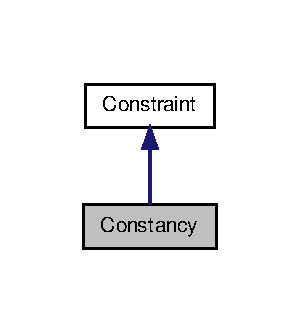
\includegraphics[width=144pt]{classConstancy__inherit__graph}
\end{center}
\end{figure}


\-Collaboration diagram for \-Constancy\-:\nopagebreak
\begin{figure}[H]
\begin{center}
\leavevmode
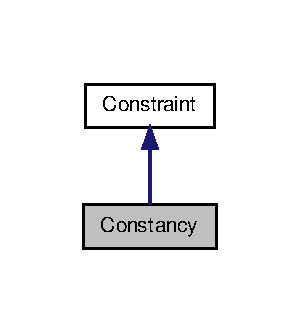
\includegraphics[width=144pt]{classConstancy__coll__graph}
\end{center}
\end{figure}
\subsection*{\-Public \-Member \-Functions}
\begin{DoxyCompactItemize}
\item 
\hyperlink{classConstancy_ae38922343ad8a98bd4e501e8ada5c83c}{\-Constancy} ()
\item 
virtual \hyperlink{classConstancy_a1cc620e04f04b406913bc60fd883bd66}{$\sim$\-Constancy} ()
\end{DoxyCompactItemize}
\subsection*{\-Protected \-Member \-Functions}
\begin{DoxyCompactItemize}
\item 
virtual void \hyperlink{classConstancy_a1759aa177ea33fab783b2b484bba8e53}{build\-Matrix\-Ci} ()
\item 
virtual void \hyperlink{classConstancy_a7d91ac4a1370d5e4a61cb2ac81dac052}{build\-Matrix\-Cii} ()
\item 
virtual void \hyperlink{classConstancy_a88e9b796f23803b9b3d2debf1be6c1e2}{build\-Vectord} ()
\end{DoxyCompactItemize}
\subsection*{\-Private \-Attributes}
\begin{DoxyCompactItemize}
\item 
\-Eigen\-::\-Vector2d \hyperlink{classConstancy_a7d416426cf6f8e9cd651d10df17c81d5}{\-\_\-\-S}
\end{DoxyCompactItemize}


\subsection{\-Constructor \& \-Destructor \-Documentation}
\hypertarget{classConstancy_ae38922343ad8a98bd4e501e8ada5c83c}{\index{\-Constancy@{\-Constancy}!\-Constancy@{\-Constancy}}
\index{\-Constancy@{\-Constancy}!Constancy@{\-Constancy}}
\subsubsection[{\-Constancy}]{\setlength{\rightskip}{0pt plus 5cm}{\bf \-Constancy\-::\-Constancy} (
\begin{DoxyParamCaption}
{}
\end{DoxyParamCaption}
)}}\label{classConstancy_ae38922343ad8a98bd4e501e8ada5c83c}
\begin{DoxyRefDesc}{\-Todo}
\item[\hyperlink{todo__todo000003}{\-Todo}]\-Upper boundaries should be input somehow from configuration file \end{DoxyRefDesc}
\hypertarget{classConstancy_a1cc620e04f04b406913bc60fd883bd66}{\index{\-Constancy@{\-Constancy}!$\sim$\-Constancy@{$\sim$\-Constancy}}
\index{$\sim$\-Constancy@{$\sim$\-Constancy}!Constancy@{\-Constancy}}
\subsubsection[{$\sim$\-Constancy}]{\setlength{\rightskip}{0pt plus 5cm}{\bf \-Constancy\-::$\sim$\-Constancy} (
\begin{DoxyParamCaption}
{}
\end{DoxyParamCaption}
)\hspace{0.3cm}{\ttfamily  \mbox{[}virtual\mbox{]}}}}\label{classConstancy_a1cc620e04f04b406913bc60fd883bd66}


\subsection{\-Member \-Function \-Documentation}
\hypertarget{classConstancy_a1759aa177ea33fab783b2b484bba8e53}{\index{\-Constancy@{\-Constancy}!build\-Matrix\-Ci@{build\-Matrix\-Ci}}
\index{build\-Matrix\-Ci@{build\-Matrix\-Ci}!Constancy@{\-Constancy}}
\subsubsection[{build\-Matrix\-Ci}]{\setlength{\rightskip}{0pt plus 5cm}void {\bf \-Constancy\-::build\-Matrix\-Ci} (
\begin{DoxyParamCaption}
{}
\end{DoxyParamCaption}
)\hspace{0.3cm}{\ttfamily  \mbox{[}protected, virtual\mbox{]}}}}\label{classConstancy_a1759aa177ea33fab783b2b484bba8e53}


\-Reimplemented from \hyperlink{classConstraint_acc08adc7b34825792cb0127a0d699269}{\-Constraint}.

\hypertarget{classConstancy_a7d91ac4a1370d5e4a61cb2ac81dac052}{\index{\-Constancy@{\-Constancy}!build\-Matrix\-Cii@{build\-Matrix\-Cii}}
\index{build\-Matrix\-Cii@{build\-Matrix\-Cii}!Constancy@{\-Constancy}}
\subsubsection[{build\-Matrix\-Cii}]{\setlength{\rightskip}{0pt plus 5cm}void {\bf \-Constancy\-::build\-Matrix\-Cii} (
\begin{DoxyParamCaption}
{}
\end{DoxyParamCaption}
)\hspace{0.3cm}{\ttfamily  \mbox{[}protected, virtual\mbox{]}}}}\label{classConstancy_a7d91ac4a1370d5e4a61cb2ac81dac052}


\-Reimplemented from \hyperlink{classConstraint_aef7c4d1071c06f34fbc5c0f06105418f}{\-Constraint}.

\hypertarget{classConstancy_a88e9b796f23803b9b3d2debf1be6c1e2}{\index{\-Constancy@{\-Constancy}!build\-Vectord@{build\-Vectord}}
\index{build\-Vectord@{build\-Vectord}!Constancy@{\-Constancy}}
\subsubsection[{build\-Vectord}]{\setlength{\rightskip}{0pt plus 5cm}void {\bf \-Constancy\-::build\-Vectord} (
\begin{DoxyParamCaption}
{}
\end{DoxyParamCaption}
)\hspace{0.3cm}{\ttfamily  \mbox{[}protected, virtual\mbox{]}}}}\label{classConstancy_a88e9b796f23803b9b3d2debf1be6c1e2}


\-Reimplemented from \hyperlink{classConstraint_a07453509c3f0f95034db965c9e699810}{\-Constraint}.



\subsection{\-Member \-Data \-Documentation}
\hypertarget{classConstancy_a7d416426cf6f8e9cd651d10df17c81d5}{\index{\-Constancy@{\-Constancy}!\-\_\-\-S@{\-\_\-\-S}}
\index{\-\_\-\-S@{\-\_\-\-S}!Constancy@{\-Constancy}}
\subsubsection[{\-\_\-\-S}]{\setlength{\rightskip}{0pt plus 5cm}\-Eigen\-::\-Vector2d {\bf \-Constancy\-::\-\_\-\-S}\hspace{0.3cm}{\ttfamily  \mbox{[}private\mbox{]}}}}\label{classConstancy_a7d416426cf6f8e9cd651d10df17c81d5}


\-The documentation for this class was generated from the following files\-:\begin{DoxyCompactItemize}
\item 
ocra-\/wbi-\/plugins/ocra-\/icub-\/clients/walking-\/client/include/walking-\/client/constraints/\hyperlink{Constancy_8h}{\-Constancy.\-h}\item 
ocra-\/wbi-\/plugins/ocra-\/icub-\/clients/walking-\/client/src/\hyperlink{Constancy_8cpp}{\-Constancy.\-cpp}\end{DoxyCompactItemize}

\hypertarget{structShapeConstraintsStruct_1_1constancyStruct}{\section{\-Shape\-Constraints\-Struct\-:\-:constancy\-Struct \-Struct \-Reference}
\label{structShapeConstraintsStruct_1_1constancyStruct}\index{\-Shape\-Constraints\-Struct\-::constancy\-Struct@{\-Shape\-Constraints\-Struct\-::constancy\-Struct}}
}


{\ttfamily \#include $<$constraints\-Structs.\-h$>$}

\subsection*{\-Public \-Attributes}
\begin{DoxyCompactItemize}
\item 
\-Eigen\-::\-Vector2d \hyperlink{structShapeConstraintsStruct_1_1constancyStruct_a5101af8a66eb956ac4734155f229f330}{\-S}
\item 
\-Eigen\-::\-Matrix\-Xd \hyperlink{structShapeConstraintsStruct_1_1constancyStruct_a703f12b002822f13a142bf468c193161}{\-C1}
\item 
\-Eigen\-::\-Matrix\-Xd \hyperlink{structShapeConstraintsStruct_1_1constancyStruct_ac2dda40a92114bf4537ed8e837258a61}{\-C2}
\item 
\-Eigen\-::\-Vector\-Xd \hyperlink{structShapeConstraintsStruct_1_1constancyStruct_a361cd12d62134f9ab3597d503bbc34b5}{d}
\item 
\-Eigen\-::\-Vector\-Xd \hyperlink{structShapeConstraintsStruct_1_1constancyStruct_a5f11451bd2f968b7ccc0905229a3f4bf}{d\-Bar}
\item 
\-Eigen\-::\-Matrix\-Xd \hyperlink{structShapeConstraintsStruct_1_1constancyStruct_aac1e5c742a7c5d837e1810722ef88351}{\-Cbar1}
\item 
\-Eigen\-::\-Matrix\-Xd \hyperlink{structShapeConstraintsStruct_1_1constancyStruct_a300bae364575fe901332ccf699e5b5e5}{\-Cbar2}
\item 
\-Eigen\-::\-Vector\-Xd \hyperlink{structShapeConstraintsStruct_1_1constancyStruct_a7dff57685375ede5909c7f732b2bdd8e}{f\-History}
\end{DoxyCompactItemize}


\subsection{\-Member \-Data \-Documentation}
\hypertarget{structShapeConstraintsStruct_1_1constancyStruct_a703f12b002822f13a142bf468c193161}{\index{\-Shape\-Constraints\-Struct\-::constancy\-Struct@{\-Shape\-Constraints\-Struct\-::constancy\-Struct}!\-C1@{\-C1}}
\index{\-C1@{\-C1}!ShapeConstraintsStruct::constancyStruct@{\-Shape\-Constraints\-Struct\-::constancy\-Struct}}
\subsubsection[{\-C1}]{\setlength{\rightskip}{0pt plus 5cm}\-Eigen\-::\-Matrix\-Xd {\bf \-Shape\-Constraints\-Struct\-::constancy\-Struct\-::\-C1}}}\label{structShapeConstraintsStruct_1_1constancyStruct_a703f12b002822f13a142bf468c193161}
\hypertarget{structShapeConstraintsStruct_1_1constancyStruct_ac2dda40a92114bf4537ed8e837258a61}{\index{\-Shape\-Constraints\-Struct\-::constancy\-Struct@{\-Shape\-Constraints\-Struct\-::constancy\-Struct}!\-C2@{\-C2}}
\index{\-C2@{\-C2}!ShapeConstraintsStruct::constancyStruct@{\-Shape\-Constraints\-Struct\-::constancy\-Struct}}
\subsubsection[{\-C2}]{\setlength{\rightskip}{0pt plus 5cm}\-Eigen\-::\-Matrix\-Xd {\bf \-Shape\-Constraints\-Struct\-::constancy\-Struct\-::\-C2}}}\label{structShapeConstraintsStruct_1_1constancyStruct_ac2dda40a92114bf4537ed8e837258a61}
\hypertarget{structShapeConstraintsStruct_1_1constancyStruct_aac1e5c742a7c5d837e1810722ef88351}{\index{\-Shape\-Constraints\-Struct\-::constancy\-Struct@{\-Shape\-Constraints\-Struct\-::constancy\-Struct}!\-Cbar1@{\-Cbar1}}
\index{\-Cbar1@{\-Cbar1}!ShapeConstraintsStruct::constancyStruct@{\-Shape\-Constraints\-Struct\-::constancy\-Struct}}
\subsubsection[{\-Cbar1}]{\setlength{\rightskip}{0pt plus 5cm}\-Eigen\-::\-Matrix\-Xd {\bf \-Shape\-Constraints\-Struct\-::constancy\-Struct\-::\-Cbar1}}}\label{structShapeConstraintsStruct_1_1constancyStruct_aac1e5c742a7c5d837e1810722ef88351}
\hypertarget{structShapeConstraintsStruct_1_1constancyStruct_a300bae364575fe901332ccf699e5b5e5}{\index{\-Shape\-Constraints\-Struct\-::constancy\-Struct@{\-Shape\-Constraints\-Struct\-::constancy\-Struct}!\-Cbar2@{\-Cbar2}}
\index{\-Cbar2@{\-Cbar2}!ShapeConstraintsStruct::constancyStruct@{\-Shape\-Constraints\-Struct\-::constancy\-Struct}}
\subsubsection[{\-Cbar2}]{\setlength{\rightskip}{0pt plus 5cm}\-Eigen\-::\-Matrix\-Xd {\bf \-Shape\-Constraints\-Struct\-::constancy\-Struct\-::\-Cbar2}}}\label{structShapeConstraintsStruct_1_1constancyStruct_a300bae364575fe901332ccf699e5b5e5}
\hypertarget{structShapeConstraintsStruct_1_1constancyStruct_a361cd12d62134f9ab3597d503bbc34b5}{\index{\-Shape\-Constraints\-Struct\-::constancy\-Struct@{\-Shape\-Constraints\-Struct\-::constancy\-Struct}!d@{d}}
\index{d@{d}!ShapeConstraintsStruct::constancyStruct@{\-Shape\-Constraints\-Struct\-::constancy\-Struct}}
\subsubsection[{d}]{\setlength{\rightskip}{0pt plus 5cm}\-Eigen\-::\-Vector\-Xd {\bf \-Shape\-Constraints\-Struct\-::constancy\-Struct\-::d}}}\label{structShapeConstraintsStruct_1_1constancyStruct_a361cd12d62134f9ab3597d503bbc34b5}
\hypertarget{structShapeConstraintsStruct_1_1constancyStruct_a5f11451bd2f968b7ccc0905229a3f4bf}{\index{\-Shape\-Constraints\-Struct\-::constancy\-Struct@{\-Shape\-Constraints\-Struct\-::constancy\-Struct}!d\-Bar@{d\-Bar}}
\index{d\-Bar@{d\-Bar}!ShapeConstraintsStruct::constancyStruct@{\-Shape\-Constraints\-Struct\-::constancy\-Struct}}
\subsubsection[{d\-Bar}]{\setlength{\rightskip}{0pt plus 5cm}\-Eigen\-::\-Vector\-Xd {\bf \-Shape\-Constraints\-Struct\-::constancy\-Struct\-::d\-Bar}}}\label{structShapeConstraintsStruct_1_1constancyStruct_a5f11451bd2f968b7ccc0905229a3f4bf}
\hypertarget{structShapeConstraintsStruct_1_1constancyStruct_a7dff57685375ede5909c7f732b2bdd8e}{\index{\-Shape\-Constraints\-Struct\-::constancy\-Struct@{\-Shape\-Constraints\-Struct\-::constancy\-Struct}!f\-History@{f\-History}}
\index{f\-History@{f\-History}!ShapeConstraintsStruct::constancyStruct@{\-Shape\-Constraints\-Struct\-::constancy\-Struct}}
\subsubsection[{f\-History}]{\setlength{\rightskip}{0pt plus 5cm}\-Eigen\-::\-Vector\-Xd {\bf \-Shape\-Constraints\-Struct\-::constancy\-Struct\-::f\-History}}}\label{structShapeConstraintsStruct_1_1constancyStruct_a7dff57685375ede5909c7f732b2bdd8e}
\hypertarget{structShapeConstraintsStruct_1_1constancyStruct_a5101af8a66eb956ac4734155f229f330}{\index{\-Shape\-Constraints\-Struct\-::constancy\-Struct@{\-Shape\-Constraints\-Struct\-::constancy\-Struct}!\-S@{\-S}}
\index{\-S@{\-S}!ShapeConstraintsStruct::constancyStruct@{\-Shape\-Constraints\-Struct\-::constancy\-Struct}}
\subsubsection[{\-S}]{\setlength{\rightskip}{0pt plus 5cm}\-Eigen\-::\-Vector2d {\bf \-Shape\-Constraints\-Struct\-::constancy\-Struct\-::\-S}}}\label{structShapeConstraintsStruct_1_1constancyStruct_a5101af8a66eb956ac4734155f229f330}


\-The documentation for this struct was generated from the following file\-:\begin{DoxyCompactItemize}
\item 
ocra-\/wbi-\/plugins/ocra-\/icub-\/clients/walking-\/client/include/walking-\/client/\hyperlink{constraintsStructs_8h}{constraints\-Structs.\-h}\end{DoxyCompactItemize}

\hypertarget{classConstraint}{\section{\-Constraint \-Class \-Reference}
\label{classConstraint}\index{\-Constraint@{\-Constraint}}
}


{\ttfamily \#include $<$\-Constraint.\-h$>$}



\-Inheritance diagram for \-Constraint\-:\nopagebreak
\begin{figure}[H]
\begin{center}
\leavevmode
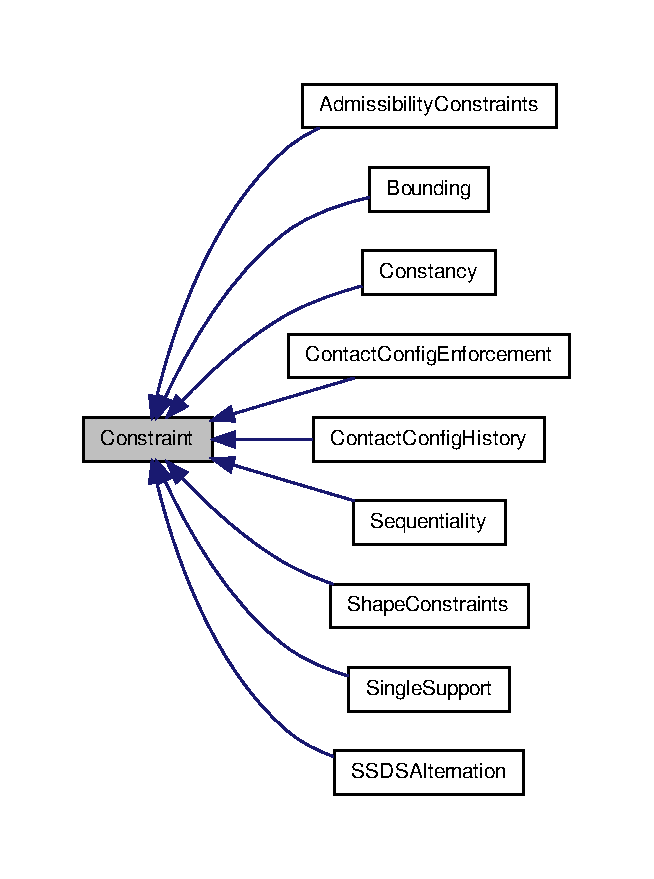
\includegraphics[width=314pt]{classConstraint__inherit__graph}
\end{center}
\end{figure}
\subsection*{\-Public \-Member \-Functions}
\begin{DoxyCompactItemize}
\item 
\hyperlink{classConstraint_ac066210c674e540f0d2570f53d6eff7b}{\-Constraint} ()
\item 
void \hyperlink{classConstraint_a0a4e0b4478205ba856dafe514d03eba4}{init} ()
\item 
\-Eigen\-::\-Matrix\-Xd \hyperlink{classConstraint_a9617822e8e1145177f41775748810ef6}{get\-Ci} ()
\item 
\-Eigen\-::\-Matrix\-Xd \hyperlink{classConstraint_abc5587e865eebb1ac924ce06e982117e}{get\-Cii} ()
\item 
\-Eigen\-::\-Vector\-Xd \hyperlink{classConstraint_a6498cc7d4a96baa9158c6e38384364d5}{getd} ()
\end{DoxyCompactItemize}
\subsection*{\-Protected \-Member \-Functions}
\begin{DoxyCompactItemize}
\item 
virtual void \hyperlink{classConstraint_acc08adc7b34825792cb0127a0d699269}{build\-Matrix\-Ci} ()
\item 
virtual void \hyperlink{classConstraint_aef7c4d1071c06f34fbc5c0f06105418f}{build\-Matrix\-Cii} ()
\item 
virtual void \hyperlink{classConstraint_a07453509c3f0f95034db965c9e699810}{build\-Vectord} ()
\end{DoxyCompactItemize}
\subsection*{\-Protected \-Attributes}
\begin{DoxyCompactItemize}
\item 
\-Eigen\-::\-Matrix\-Xd \hyperlink{classConstraint_a71217c52597267a96e6bd2d9ed48740f}{\-\_\-\-Ci}
\item 
\-Eigen\-::\-Matrix\-Xd \hyperlink{classConstraint_a6cc83eda35602acec07aab75e9f209dd}{\-\_\-\-Cii}
\item 
\-Eigen\-::\-Vector\-Xd \hyperlink{classConstraint_a97db6afdcd2827da0dbe3a4e6cd13b7f}{\-\_\-d}
\end{DoxyCompactItemize}


\subsection{\-Constructor \& \-Destructor \-Documentation}
\hypertarget{classConstraint_ac066210c674e540f0d2570f53d6eff7b}{\index{\-Constraint@{\-Constraint}!\-Constraint@{\-Constraint}}
\index{\-Constraint@{\-Constraint}!Constraint@{\-Constraint}}
\subsubsection[{\-Constraint}]{\setlength{\rightskip}{0pt plus 5cm}{\bf \-Constraint\-::\-Constraint} (
\begin{DoxyParamCaption}
{}
\end{DoxyParamCaption}
)\hspace{0.3cm}{\ttfamily  \mbox{[}inline\mbox{]}}}}\label{classConstraint_ac066210c674e540f0d2570f53d6eff7b}


\subsection{\-Member \-Function \-Documentation}
\hypertarget{classConstraint_acc08adc7b34825792cb0127a0d699269}{\index{\-Constraint@{\-Constraint}!build\-Matrix\-Ci@{build\-Matrix\-Ci}}
\index{build\-Matrix\-Ci@{build\-Matrix\-Ci}!Constraint@{\-Constraint}}
\subsubsection[{build\-Matrix\-Ci}]{\setlength{\rightskip}{0pt plus 5cm}virtual void {\bf \-Constraint\-::build\-Matrix\-Ci} (
\begin{DoxyParamCaption}
{}
\end{DoxyParamCaption}
)\hspace{0.3cm}{\ttfamily  \mbox{[}inline, protected, virtual\mbox{]}}}}\label{classConstraint_acc08adc7b34825792cb0127a0d699269}


\-Reimplemented in \hyperlink{classAdmissibilityConstraints_a22333fbffb9df28433e066b5a00a9c00}{\-Admissibility\-Constraints}, \hyperlink{classShapeConstraints_a5106b5a5d1b55e1751423f2af1102c4e}{\-Shape\-Constraints}, \hyperlink{classSingleSupport_a78e5b7c89b828d718560cec73c0f6218}{\-Single\-Support}, \hyperlink{classConstancy_a1759aa177ea33fab783b2b484bba8e53}{\-Constancy}, \hyperlink{classContactConfigEnforcement_aca7e59b45bc72557872cd9a12a202a5e}{\-Contact\-Config\-Enforcement}, \hyperlink{classContactConfigHistory_a2bd6c647990ab8fd81f48461a144de73}{\-Contact\-Config\-History}, \hyperlink{classBounding_a3997be7d9301b6e353daf574ce307462}{\-Bounding}, \hyperlink{classSSDSAlternation_af4e463bf49d5863366c38de3e3f5e74b}{\-S\-S\-D\-S\-Alternation}, and \hyperlink{classSequentiality_a9244bd4d6ff9fe4528658b2adc53fb13}{\-Sequentiality}.

\hypertarget{classConstraint_aef7c4d1071c06f34fbc5c0f06105418f}{\index{\-Constraint@{\-Constraint}!build\-Matrix\-Cii@{build\-Matrix\-Cii}}
\index{build\-Matrix\-Cii@{build\-Matrix\-Cii}!Constraint@{\-Constraint}}
\subsubsection[{build\-Matrix\-Cii}]{\setlength{\rightskip}{0pt plus 5cm}virtual void {\bf \-Constraint\-::build\-Matrix\-Cii} (
\begin{DoxyParamCaption}
{}
\end{DoxyParamCaption}
)\hspace{0.3cm}{\ttfamily  \mbox{[}inline, protected, virtual\mbox{]}}}}\label{classConstraint_aef7c4d1071c06f34fbc5c0f06105418f}


\-Reimplemented in \hyperlink{classAdmissibilityConstraints_a98de6682160b1161d0eb57852ccfce25}{\-Admissibility\-Constraints}, \hyperlink{classShapeConstraints_a22fcfce709900f384603a759729bdbcd}{\-Shape\-Constraints}, \hyperlink{classSingleSupport_a746b653c7fbbe989032dadbcfdae3193}{\-Single\-Support}, \hyperlink{classConstancy_a7d91ac4a1370d5e4a61cb2ac81dac052}{\-Constancy}, \hyperlink{classContactConfigEnforcement_a37bf7472b54d88ea95c9d20d342fb9cf}{\-Contact\-Config\-Enforcement}, \hyperlink{classContactConfigHistory_adff0b3c563ac91b5d81f07ac758f1b7c}{\-Contact\-Config\-History}, \hyperlink{classBounding_a885a21bf71462c1c4bbb200d4266ca94}{\-Bounding}, \hyperlink{classSSDSAlternation_aa527e6b2639391ccd602392e7dceba1e}{\-S\-S\-D\-S\-Alternation}, and \hyperlink{classSequentiality_a241b1688f3da2e5accf6ee0799e1c95b}{\-Sequentiality}.

\hypertarget{classConstraint_a07453509c3f0f95034db965c9e699810}{\index{\-Constraint@{\-Constraint}!build\-Vectord@{build\-Vectord}}
\index{build\-Vectord@{build\-Vectord}!Constraint@{\-Constraint}}
\subsubsection[{build\-Vectord}]{\setlength{\rightskip}{0pt plus 5cm}virtual void {\bf \-Constraint\-::build\-Vectord} (
\begin{DoxyParamCaption}
{}
\end{DoxyParamCaption}
)\hspace{0.3cm}{\ttfamily  \mbox{[}inline, protected, virtual\mbox{]}}}}\label{classConstraint_a07453509c3f0f95034db965c9e699810}


\-Reimplemented in \hyperlink{classAdmissibilityConstraints_a48f89a09f8c9607925652622a8c70fb4}{\-Admissibility\-Constraints}, \hyperlink{classShapeConstraints_ad7fa37ff0da8688ec2f51add0731a232}{\-Shape\-Constraints}, \hyperlink{classSingleSupport_a43caf4b390371ce015cec54d5e78759d}{\-Single\-Support}, \hyperlink{classConstancy_a88e9b796f23803b9b3d2debf1be6c1e2}{\-Constancy}, \hyperlink{classContactConfigEnforcement_a6ef8fa159fbaa7add701b6d577506244}{\-Contact\-Config\-Enforcement}, \hyperlink{classContactConfigHistory_abfdb78174a3294565a3a6059cfab09f5}{\-Contact\-Config\-History}, \hyperlink{classBounding_a2d1a349549b5b0633fb7a5c338cb5cf6}{\-Bounding}, \hyperlink{classSSDSAlternation_ac081b561d5553ca392157304662b3b13}{\-S\-S\-D\-S\-Alternation}, and \hyperlink{classSequentiality_ae115049b18674543e1a7ca2fad039e4b}{\-Sequentiality}.

\hypertarget{classConstraint_a9617822e8e1145177f41775748810ef6}{\index{\-Constraint@{\-Constraint}!get\-Ci@{get\-Ci}}
\index{get\-Ci@{get\-Ci}!Constraint@{\-Constraint}}
\subsubsection[{get\-Ci}]{\setlength{\rightskip}{0pt plus 5cm}\-Eigen\-::\-Matrix\-Xd {\bf \-Constraint\-::get\-Ci} (
\begin{DoxyParamCaption}
{}
\end{DoxyParamCaption}
)\hspace{0.3cm}{\ttfamily  \mbox{[}inline\mbox{]}}}}\label{classConstraint_a9617822e8e1145177f41775748810ef6}
\hypertarget{classConstraint_abc5587e865eebb1ac924ce06e982117e}{\index{\-Constraint@{\-Constraint}!get\-Cii@{get\-Cii}}
\index{get\-Cii@{get\-Cii}!Constraint@{\-Constraint}}
\subsubsection[{get\-Cii}]{\setlength{\rightskip}{0pt plus 5cm}\-Eigen\-::\-Matrix\-Xd {\bf \-Constraint\-::get\-Cii} (
\begin{DoxyParamCaption}
{}
\end{DoxyParamCaption}
)\hspace{0.3cm}{\ttfamily  \mbox{[}inline\mbox{]}}}}\label{classConstraint_abc5587e865eebb1ac924ce06e982117e}
\hypertarget{classConstraint_a6498cc7d4a96baa9158c6e38384364d5}{\index{\-Constraint@{\-Constraint}!getd@{getd}}
\index{getd@{getd}!Constraint@{\-Constraint}}
\subsubsection[{getd}]{\setlength{\rightskip}{0pt plus 5cm}\-Eigen\-::\-Vector\-Xd {\bf \-Constraint\-::getd} (
\begin{DoxyParamCaption}
{}
\end{DoxyParamCaption}
)\hspace{0.3cm}{\ttfamily  \mbox{[}inline\mbox{]}}}}\label{classConstraint_a6498cc7d4a96baa9158c6e38384364d5}
\hypertarget{classConstraint_a0a4e0b4478205ba856dafe514d03eba4}{\index{\-Constraint@{\-Constraint}!init@{init}}
\index{init@{init}!Constraint@{\-Constraint}}
\subsubsection[{init}]{\setlength{\rightskip}{0pt plus 5cm}void {\bf \-Constraint\-::init} (
\begin{DoxyParamCaption}
{}
\end{DoxyParamCaption}
)\hspace{0.3cm}{\ttfamily  \mbox{[}inline\mbox{]}}}}\label{classConstraint_a0a4e0b4478205ba856dafe514d03eba4}


\subsection{\-Member \-Data \-Documentation}
\hypertarget{classConstraint_a71217c52597267a96e6bd2d9ed48740f}{\index{\-Constraint@{\-Constraint}!\-\_\-\-Ci@{\-\_\-\-Ci}}
\index{\-\_\-\-Ci@{\-\_\-\-Ci}!Constraint@{\-Constraint}}
\subsubsection[{\-\_\-\-Ci}]{\setlength{\rightskip}{0pt plus 5cm}\-Eigen\-::\-Matrix\-Xd {\bf \-Constraint\-::\-\_\-\-Ci}\hspace{0.3cm}{\ttfamily  \mbox{[}protected\mbox{]}}}}\label{classConstraint_a71217c52597267a96e6bd2d9ed48740f}
\hypertarget{classConstraint_a6cc83eda35602acec07aab75e9f209dd}{\index{\-Constraint@{\-Constraint}!\-\_\-\-Cii@{\-\_\-\-Cii}}
\index{\-\_\-\-Cii@{\-\_\-\-Cii}!Constraint@{\-Constraint}}
\subsubsection[{\-\_\-\-Cii}]{\setlength{\rightskip}{0pt plus 5cm}\-Eigen\-::\-Matrix\-Xd {\bf \-Constraint\-::\-\_\-\-Cii}\hspace{0.3cm}{\ttfamily  \mbox{[}protected\mbox{]}}}}\label{classConstraint_a6cc83eda35602acec07aab75e9f209dd}
\hypertarget{classConstraint_a97db6afdcd2827da0dbe3a4e6cd13b7f}{\index{\-Constraint@{\-Constraint}!\-\_\-d@{\-\_\-d}}
\index{\-\_\-d@{\-\_\-d}!Constraint@{\-Constraint}}
\subsubsection[{\-\_\-d}]{\setlength{\rightskip}{0pt plus 5cm}\-Eigen\-::\-Vector\-Xd {\bf \-Constraint\-::\-\_\-d}\hspace{0.3cm}{\ttfamily  \mbox{[}protected\mbox{]}}}}\label{classConstraint_a97db6afdcd2827da0dbe3a4e6cd13b7f}


\-The documentation for this class was generated from the following file\-:\begin{DoxyCompactItemize}
\item 
ocra-\/wbi-\/plugins/ocra-\/icub-\/clients/walking-\/client/include/walking-\/client/constraints/\hyperlink{Constraint_8h}{\-Constraint.\-h}\end{DoxyCompactItemize}

\hypertarget{classContactConfigEnforcement}{\section{\-Contact\-Config\-Enforcement \-Class \-Reference}
\label{classContactConfigEnforcement}\index{\-Contact\-Config\-Enforcement@{\-Contact\-Config\-Enforcement}}
}


{\ttfamily \#include $<$\-Contact\-Config\-Enforcement.\-h$>$}



\-Inheritance diagram for \-Contact\-Config\-Enforcement\-:
\nopagebreak
\begin{figure}[H]
\begin{center}
\leavevmode
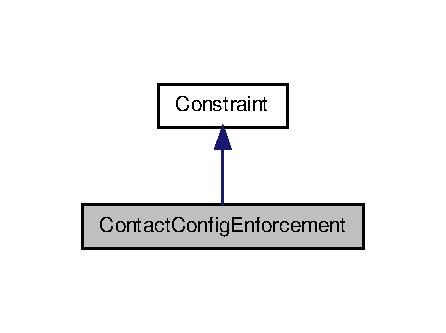
\includegraphics[width=214pt]{classContactConfigEnforcement__inherit__graph}
\end{center}
\end{figure}


\-Collaboration diagram for \-Contact\-Config\-Enforcement\-:
\nopagebreak
\begin{figure}[H]
\begin{center}
\leavevmode
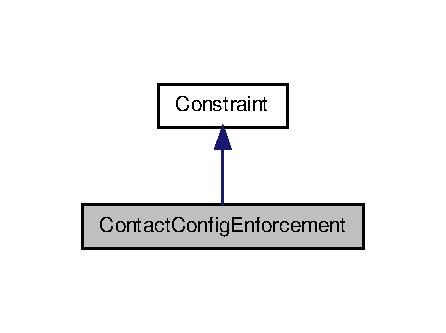
\includegraphics[width=214pt]{classContactConfigEnforcement__coll__graph}
\end{center}
\end{figure}
\subsection*{\-Public \-Member \-Functions}
\begin{DoxyCompactItemize}
\item 
\hyperlink{classContactConfigEnforcement_affa2663e090bfc8ba63b2a32a31f1707}{\-Contact\-Config\-Enforcement} ()
\item 
virtual \hyperlink{classContactConfigEnforcement_a8a58b4c421e538be35979680c96fd1d9}{$\sim$\-Contact\-Config\-Enforcement} ()
\end{DoxyCompactItemize}
\subsection*{\-Protected \-Member \-Functions}
\begin{DoxyCompactItemize}
\item 
void \hyperlink{classContactConfigEnforcement_aca7e59b45bc72557872cd9a12a202a5e}{build\-Matrix\-Ci} ()
\item 
void \hyperlink{classContactConfigEnforcement_a37bf7472b54d88ea95c9d20d342fb9cf}{build\-Matrix\-Cii} ()
\item 
void \hyperlink{classContactConfigEnforcement_a6ef8fa159fbaa7add701b6d577506244}{build\-Vectord} ()
\end{DoxyCompactItemize}


\subsection{\-Constructor \& \-Destructor \-Documentation}
\hypertarget{classContactConfigEnforcement_affa2663e090bfc8ba63b2a32a31f1707}{\index{\-Contact\-Config\-Enforcement@{\-Contact\-Config\-Enforcement}!\-Contact\-Config\-Enforcement@{\-Contact\-Config\-Enforcement}}
\index{\-Contact\-Config\-Enforcement@{\-Contact\-Config\-Enforcement}!ContactConfigEnforcement@{\-Contact\-Config\-Enforcement}}
\subsubsection[{\-Contact\-Config\-Enforcement}]{\setlength{\rightskip}{0pt plus 5cm}{\bf \-Contact\-Config\-Enforcement\-::\-Contact\-Config\-Enforcement} (
\begin{DoxyParamCaption}
{}
\end{DoxyParamCaption}
)}}\label{classContactConfigEnforcement_affa2663e090bfc8ba63b2a32a31f1707}
\hypertarget{classContactConfigEnforcement_a8a58b4c421e538be35979680c96fd1d9}{\index{\-Contact\-Config\-Enforcement@{\-Contact\-Config\-Enforcement}!$\sim$\-Contact\-Config\-Enforcement@{$\sim$\-Contact\-Config\-Enforcement}}
\index{$\sim$\-Contact\-Config\-Enforcement@{$\sim$\-Contact\-Config\-Enforcement}!ContactConfigEnforcement@{\-Contact\-Config\-Enforcement}}
\subsubsection[{$\sim$\-Contact\-Config\-Enforcement}]{\setlength{\rightskip}{0pt plus 5cm}{\bf \-Contact\-Config\-Enforcement\-::$\sim$\-Contact\-Config\-Enforcement} (
\begin{DoxyParamCaption}
{}
\end{DoxyParamCaption}
)\hspace{0.3cm}{\ttfamily  \mbox{[}virtual\mbox{]}}}}\label{classContactConfigEnforcement_a8a58b4c421e538be35979680c96fd1d9}


\subsection{\-Member \-Function \-Documentation}
\hypertarget{classContactConfigEnforcement_aca7e59b45bc72557872cd9a12a202a5e}{\index{\-Contact\-Config\-Enforcement@{\-Contact\-Config\-Enforcement}!build\-Matrix\-Ci@{build\-Matrix\-Ci}}
\index{build\-Matrix\-Ci@{build\-Matrix\-Ci}!ContactConfigEnforcement@{\-Contact\-Config\-Enforcement}}
\subsubsection[{build\-Matrix\-Ci}]{\setlength{\rightskip}{0pt plus 5cm}void {\bf \-Contact\-Config\-Enforcement\-::build\-Matrix\-Ci} (
\begin{DoxyParamCaption}
{}
\end{DoxyParamCaption}
)\hspace{0.3cm}{\ttfamily  \mbox{[}protected, virtual\mbox{]}}}}\label{classContactConfigEnforcement_aca7e59b45bc72557872cd9a12a202a5e}


\-Reimplemented from \hyperlink{classConstraint_acc08adc7b34825792cb0127a0d699269}{\-Constraint}.

\hypertarget{classContactConfigEnforcement_a37bf7472b54d88ea95c9d20d342fb9cf}{\index{\-Contact\-Config\-Enforcement@{\-Contact\-Config\-Enforcement}!build\-Matrix\-Cii@{build\-Matrix\-Cii}}
\index{build\-Matrix\-Cii@{build\-Matrix\-Cii}!ContactConfigEnforcement@{\-Contact\-Config\-Enforcement}}
\subsubsection[{build\-Matrix\-Cii}]{\setlength{\rightskip}{0pt plus 5cm}void {\bf \-Contact\-Config\-Enforcement\-::build\-Matrix\-Cii} (
\begin{DoxyParamCaption}
{}
\end{DoxyParamCaption}
)\hspace{0.3cm}{\ttfamily  \mbox{[}protected, virtual\mbox{]}}}}\label{classContactConfigEnforcement_a37bf7472b54d88ea95c9d20d342fb9cf}


\-Reimplemented from \hyperlink{classConstraint_aef7c4d1071c06f34fbc5c0f06105418f}{\-Constraint}.

\hypertarget{classContactConfigEnforcement_a6ef8fa159fbaa7add701b6d577506244}{\index{\-Contact\-Config\-Enforcement@{\-Contact\-Config\-Enforcement}!build\-Vectord@{build\-Vectord}}
\index{build\-Vectord@{build\-Vectord}!ContactConfigEnforcement@{\-Contact\-Config\-Enforcement}}
\subsubsection[{build\-Vectord}]{\setlength{\rightskip}{0pt plus 5cm}void {\bf \-Contact\-Config\-Enforcement\-::build\-Vectord} (
\begin{DoxyParamCaption}
{}
\end{DoxyParamCaption}
)\hspace{0.3cm}{\ttfamily  \mbox{[}protected, virtual\mbox{]}}}}\label{classContactConfigEnforcement_a6ef8fa159fbaa7add701b6d577506244}


\-Reimplemented from \hyperlink{classConstraint_a07453509c3f0f95034db965c9e699810}{\-Constraint}.



\-The documentation for this class was generated from the following files\-:\begin{DoxyCompactItemize}
\item 
ocra-\/wbi-\/plugins/ocra-\/icub-\/clients/walking-\/client/include/walking-\/client/constraints/\hyperlink{ContactConfigEnforcement_8h}{\-Contact\-Config\-Enforcement.\-h}\item 
ocra-\/wbi-\/plugins/ocra-\/icub-\/clients/walking-\/client/src/\hyperlink{ContactConfigEnforcement_8cpp}{\-Contact\-Config\-Enforcement.\-cpp}\end{DoxyCompactItemize}

\hypertarget{classContactConfigHistory}{\section{\-Contact\-Config\-History \-Class \-Reference}
\label{classContactConfigHistory}\index{\-Contact\-Config\-History@{\-Contact\-Config\-History}}
}


{\ttfamily \#include $<$\-Contact\-Config\-History.\-h$>$}



\-Inheritance diagram for \-Contact\-Config\-History\-:
\nopagebreak
\begin{figure}[H]
\begin{center}
\leavevmode
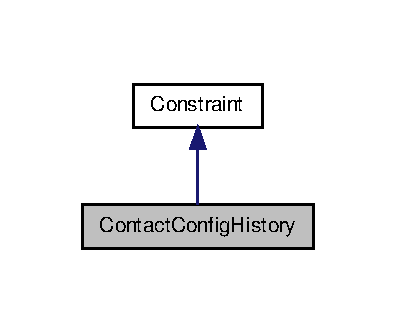
\includegraphics[width=190pt]{classContactConfigHistory__inherit__graph}
\end{center}
\end{figure}


\-Collaboration diagram for \-Contact\-Config\-History\-:
\nopagebreak
\begin{figure}[H]
\begin{center}
\leavevmode
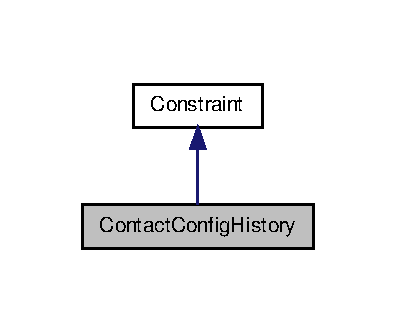
\includegraphics[width=190pt]{classContactConfigHistory__coll__graph}
\end{center}
\end{figure}
\subsection*{\-Public \-Member \-Functions}
\begin{DoxyCompactItemize}
\item 
\hyperlink{classContactConfigHistory_aa2ff8c4c2b05ca2168c5ea61bfbeb9ec}{\-Contact\-Config\-History} ()
\item 
virtual \hyperlink{classContactConfigHistory_a2b84c6e1ed477c052a18c0933c3988cf}{$\sim$\-Contact\-Config\-History} ()
\end{DoxyCompactItemize}
\subsection*{\-Protected \-Member \-Functions}
\begin{DoxyCompactItemize}
\item 
void \hyperlink{classContactConfigHistory_a2bd6c647990ab8fd81f48461a144de73}{build\-Matrix\-Ci} ()
\item 
void \hyperlink{classContactConfigHistory_adff0b3c563ac91b5d81f07ac758f1b7c}{build\-Matrix\-Cii} ()
\item 
void \hyperlink{classContactConfigHistory_abfdb78174a3294565a3a6059cfab09f5}{build\-Vectord} ()
\end{DoxyCompactItemize}


\subsection{\-Constructor \& \-Destructor \-Documentation}
\hypertarget{classContactConfigHistory_aa2ff8c4c2b05ca2168c5ea61bfbeb9ec}{\index{\-Contact\-Config\-History@{\-Contact\-Config\-History}!\-Contact\-Config\-History@{\-Contact\-Config\-History}}
\index{\-Contact\-Config\-History@{\-Contact\-Config\-History}!ContactConfigHistory@{\-Contact\-Config\-History}}
\subsubsection[{\-Contact\-Config\-History}]{\setlength{\rightskip}{0pt plus 5cm}{\bf \-Contact\-Config\-History\-::\-Contact\-Config\-History} (
\begin{DoxyParamCaption}
{}
\end{DoxyParamCaption}
)}}\label{classContactConfigHistory_aa2ff8c4c2b05ca2168c5ea61bfbeb9ec}
\hypertarget{classContactConfigHistory_a2b84c6e1ed477c052a18c0933c3988cf}{\index{\-Contact\-Config\-History@{\-Contact\-Config\-History}!$\sim$\-Contact\-Config\-History@{$\sim$\-Contact\-Config\-History}}
\index{$\sim$\-Contact\-Config\-History@{$\sim$\-Contact\-Config\-History}!ContactConfigHistory@{\-Contact\-Config\-History}}
\subsubsection[{$\sim$\-Contact\-Config\-History}]{\setlength{\rightskip}{0pt plus 5cm}{\bf \-Contact\-Config\-History\-::$\sim$\-Contact\-Config\-History} (
\begin{DoxyParamCaption}
{}
\end{DoxyParamCaption}
)\hspace{0.3cm}{\ttfamily  \mbox{[}virtual\mbox{]}}}}\label{classContactConfigHistory_a2b84c6e1ed477c052a18c0933c3988cf}


\subsection{\-Member \-Function \-Documentation}
\hypertarget{classContactConfigHistory_a2bd6c647990ab8fd81f48461a144de73}{\index{\-Contact\-Config\-History@{\-Contact\-Config\-History}!build\-Matrix\-Ci@{build\-Matrix\-Ci}}
\index{build\-Matrix\-Ci@{build\-Matrix\-Ci}!ContactConfigHistory@{\-Contact\-Config\-History}}
\subsubsection[{build\-Matrix\-Ci}]{\setlength{\rightskip}{0pt plus 5cm}void {\bf \-Contact\-Config\-History\-::build\-Matrix\-Ci} (
\begin{DoxyParamCaption}
{}
\end{DoxyParamCaption}
)\hspace{0.3cm}{\ttfamily  \mbox{[}protected, virtual\mbox{]}}}}\label{classContactConfigHistory_a2bd6c647990ab8fd81f48461a144de73}


\-Reimplemented from \hyperlink{classConstraint_acc08adc7b34825792cb0127a0d699269}{\-Constraint}.

\hypertarget{classContactConfigHistory_adff0b3c563ac91b5d81f07ac758f1b7c}{\index{\-Contact\-Config\-History@{\-Contact\-Config\-History}!build\-Matrix\-Cii@{build\-Matrix\-Cii}}
\index{build\-Matrix\-Cii@{build\-Matrix\-Cii}!ContactConfigHistory@{\-Contact\-Config\-History}}
\subsubsection[{build\-Matrix\-Cii}]{\setlength{\rightskip}{0pt plus 5cm}void {\bf \-Contact\-Config\-History\-::build\-Matrix\-Cii} (
\begin{DoxyParamCaption}
{}
\end{DoxyParamCaption}
)\hspace{0.3cm}{\ttfamily  \mbox{[}protected, virtual\mbox{]}}}}\label{classContactConfigHistory_adff0b3c563ac91b5d81f07ac758f1b7c}


\-Reimplemented from \hyperlink{classConstraint_aef7c4d1071c06f34fbc5c0f06105418f}{\-Constraint}.

\hypertarget{classContactConfigHistory_abfdb78174a3294565a3a6059cfab09f5}{\index{\-Contact\-Config\-History@{\-Contact\-Config\-History}!build\-Vectord@{build\-Vectord}}
\index{build\-Vectord@{build\-Vectord}!ContactConfigHistory@{\-Contact\-Config\-History}}
\subsubsection[{build\-Vectord}]{\setlength{\rightskip}{0pt plus 5cm}void {\bf \-Contact\-Config\-History\-::build\-Vectord} (
\begin{DoxyParamCaption}
{}
\end{DoxyParamCaption}
)\hspace{0.3cm}{\ttfamily  \mbox{[}protected, virtual\mbox{]}}}}\label{classContactConfigHistory_abfdb78174a3294565a3a6059cfab09f5}


\-Reimplemented from \hyperlink{classConstraint_a07453509c3f0f95034db965c9e699810}{\-Constraint}.



\-The documentation for this class was generated from the following files\-:\begin{DoxyCompactItemize}
\item 
ocra-\/wbi-\/plugins/ocra-\/icub-\/clients/walking-\/client/include/walking-\/client/constraints/\hyperlink{ContactConfigHistory_8h}{\-Contact\-Config\-History.\-h}\item 
ocra-\/wbi-\/plugins/ocra-\/icub-\/clients/walking-\/client/src/\hyperlink{ContactConfigHistory_8cpp}{\-Contact\-Config\-History.\-cpp}\end{DoxyCompactItemize}

\hypertarget{structAdmissibilityConstraintsStruct_1_1ContactConfigurationEnforcement}{\section{\-Admissibility\-Constraints\-Struct\-:\-:\-Contact\-Configuration\-Enforcement \-Struct \-Reference}
\label{structAdmissibilityConstraintsStruct_1_1ContactConfigurationEnforcement}\index{\-Admissibility\-Constraints\-Struct\-::\-Contact\-Configuration\-Enforcement@{\-Admissibility\-Constraints\-Struct\-::\-Contact\-Configuration\-Enforcement}}
}


{\ttfamily \#include $<$constraints\-Structs.\-h$>$}

\subsection*{\-Public \-Attributes}
\begin{DoxyCompactItemize}
\item 
\-Eigen\-::\-Matrix\-Xd \hyperlink{structAdmissibilityConstraintsStruct_1_1ContactConfigurationEnforcement_a6688d4bb3e397219074bcf5699ffca55}{\-C}
\item 
\-Eigen\-::\-Vector\-Xd \hyperlink{structAdmissibilityConstraintsStruct_1_1ContactConfigurationEnforcement_a43ec5c057d018f841c08a82d3806c6b4}{d}
\item 
\-Eigen\-::\-Matrix\-Xd \hyperlink{structAdmissibilityConstraintsStruct_1_1ContactConfigurationEnforcement_a60be82cc4c6c03f69a6b01a4a210dbec}{\-Cbar}
\item 
\-Eigen\-::\-Vector\-Xd \hyperlink{structAdmissibilityConstraintsStruct_1_1ContactConfigurationEnforcement_a0061c6cddeac4d3cb4d5bfc68cb21026}{d\-Bar}
\item 
\-Eigen\-::\-Vector\-Xd \hyperlink{structAdmissibilityConstraintsStruct_1_1ContactConfigurationEnforcement_a3ca6a4f62e9f1c5c5465fce49020a72b}{f\-History}
\end{DoxyCompactItemize}


\subsection{\-Member \-Data \-Documentation}
\hypertarget{structAdmissibilityConstraintsStruct_1_1ContactConfigurationEnforcement_a6688d4bb3e397219074bcf5699ffca55}{\index{\-Admissibility\-Constraints\-Struct\-::\-Contact\-Configuration\-Enforcement@{\-Admissibility\-Constraints\-Struct\-::\-Contact\-Configuration\-Enforcement}!\-C@{\-C}}
\index{\-C@{\-C}!AdmissibilityConstraintsStruct::ContactConfigurationEnforcement@{\-Admissibility\-Constraints\-Struct\-::\-Contact\-Configuration\-Enforcement}}
\subsubsection[{\-C}]{\setlength{\rightskip}{0pt plus 5cm}\-Eigen\-::\-Matrix\-Xd {\bf \-Admissibility\-Constraints\-Struct\-::\-Contact\-Configuration\-Enforcement\-::\-C}}}\label{structAdmissibilityConstraintsStruct_1_1ContactConfigurationEnforcement_a6688d4bb3e397219074bcf5699ffca55}
\hypertarget{structAdmissibilityConstraintsStruct_1_1ContactConfigurationEnforcement_a60be82cc4c6c03f69a6b01a4a210dbec}{\index{\-Admissibility\-Constraints\-Struct\-::\-Contact\-Configuration\-Enforcement@{\-Admissibility\-Constraints\-Struct\-::\-Contact\-Configuration\-Enforcement}!\-Cbar@{\-Cbar}}
\index{\-Cbar@{\-Cbar}!AdmissibilityConstraintsStruct::ContactConfigurationEnforcement@{\-Admissibility\-Constraints\-Struct\-::\-Contact\-Configuration\-Enforcement}}
\subsubsection[{\-Cbar}]{\setlength{\rightskip}{0pt plus 5cm}\-Eigen\-::\-Matrix\-Xd {\bf \-Admissibility\-Constraints\-Struct\-::\-Contact\-Configuration\-Enforcement\-::\-Cbar}}}\label{structAdmissibilityConstraintsStruct_1_1ContactConfigurationEnforcement_a60be82cc4c6c03f69a6b01a4a210dbec}
\hypertarget{structAdmissibilityConstraintsStruct_1_1ContactConfigurationEnforcement_a43ec5c057d018f841c08a82d3806c6b4}{\index{\-Admissibility\-Constraints\-Struct\-::\-Contact\-Configuration\-Enforcement@{\-Admissibility\-Constraints\-Struct\-::\-Contact\-Configuration\-Enforcement}!d@{d}}
\index{d@{d}!AdmissibilityConstraintsStruct::ContactConfigurationEnforcement@{\-Admissibility\-Constraints\-Struct\-::\-Contact\-Configuration\-Enforcement}}
\subsubsection[{d}]{\setlength{\rightskip}{0pt plus 5cm}\-Eigen\-::\-Vector\-Xd {\bf \-Admissibility\-Constraints\-Struct\-::\-Contact\-Configuration\-Enforcement\-::d}}}\label{structAdmissibilityConstraintsStruct_1_1ContactConfigurationEnforcement_a43ec5c057d018f841c08a82d3806c6b4}
\hypertarget{structAdmissibilityConstraintsStruct_1_1ContactConfigurationEnforcement_a0061c6cddeac4d3cb4d5bfc68cb21026}{\index{\-Admissibility\-Constraints\-Struct\-::\-Contact\-Configuration\-Enforcement@{\-Admissibility\-Constraints\-Struct\-::\-Contact\-Configuration\-Enforcement}!d\-Bar@{d\-Bar}}
\index{d\-Bar@{d\-Bar}!AdmissibilityConstraintsStruct::ContactConfigurationEnforcement@{\-Admissibility\-Constraints\-Struct\-::\-Contact\-Configuration\-Enforcement}}
\subsubsection[{d\-Bar}]{\setlength{\rightskip}{0pt plus 5cm}\-Eigen\-::\-Vector\-Xd {\bf \-Admissibility\-Constraints\-Struct\-::\-Contact\-Configuration\-Enforcement\-::d\-Bar}}}\label{structAdmissibilityConstraintsStruct_1_1ContactConfigurationEnforcement_a0061c6cddeac4d3cb4d5bfc68cb21026}
\hypertarget{structAdmissibilityConstraintsStruct_1_1ContactConfigurationEnforcement_a3ca6a4f62e9f1c5c5465fce49020a72b}{\index{\-Admissibility\-Constraints\-Struct\-::\-Contact\-Configuration\-Enforcement@{\-Admissibility\-Constraints\-Struct\-::\-Contact\-Configuration\-Enforcement}!f\-History@{f\-History}}
\index{f\-History@{f\-History}!AdmissibilityConstraintsStruct::ContactConfigurationEnforcement@{\-Admissibility\-Constraints\-Struct\-::\-Contact\-Configuration\-Enforcement}}
\subsubsection[{f\-History}]{\setlength{\rightskip}{0pt plus 5cm}\-Eigen\-::\-Vector\-Xd {\bf \-Admissibility\-Constraints\-Struct\-::\-Contact\-Configuration\-Enforcement\-::f\-History}}}\label{structAdmissibilityConstraintsStruct_1_1ContactConfigurationEnforcement_a3ca6a4f62e9f1c5c5465fce49020a72b}


\-The documentation for this struct was generated from the following file\-:\begin{DoxyCompactItemize}
\item 
ocra-\/wbi-\/plugins/ocra-\/icub-\/clients/walking-\/client/include/walking-\/client/\hyperlink{constraintsStructs_8h}{constraints\-Structs.\-h}\end{DoxyCompactItemize}

\hypertarget{structAdmissibilityConstraintsStruct_1_1ContactConfigurationHistory}{\section{\-Admissibility\-Constraints\-Struct\-:\-:\-Contact\-Configuration\-History \-Struct \-Reference}
\label{structAdmissibilityConstraintsStruct_1_1ContactConfigurationHistory}\index{\-Admissibility\-Constraints\-Struct\-::\-Contact\-Configuration\-History@{\-Admissibility\-Constraints\-Struct\-::\-Contact\-Configuration\-History}}
}


{\ttfamily \#include $<$constraints\-Structs.\-h$>$}

\subsection*{\-Public \-Attributes}
\begin{DoxyCompactItemize}
\item 
\-Eigen\-::\-Matrix\-Xd \hyperlink{structAdmissibilityConstraintsStruct_1_1ContactConfigurationHistory_a4111821b74104d00eb0c38e9177a5895}{\-C1}
\item 
\-Eigen\-::\-Matrix\-Xd \hyperlink{structAdmissibilityConstraintsStruct_1_1ContactConfigurationHistory_abd720b4028504806284818eab2e4c29a}{\-C2}
\item 
\-Eigen\-::\-Vector\-Xd \hyperlink{structAdmissibilityConstraintsStruct_1_1ContactConfigurationHistory_a6fa1f1664c5ac71f5d3ae1d0a4e95ec8}{d}
\item 
\-Eigen\-::\-Matrix\-Xd \hyperlink{structAdmissibilityConstraintsStruct_1_1ContactConfigurationHistory_ab80b3c301eae49e2c8705698c3e5dbc0}{\-C1bar}
\item 
\-Eigen\-::\-Matrix\-Xd \hyperlink{structAdmissibilityConstraintsStruct_1_1ContactConfigurationHistory_a61b1a4784607faf5a6bebd0422a215f8}{\-C2bar}
\item 
\-Eigen\-::\-Vector\-Xd \hyperlink{structAdmissibilityConstraintsStruct_1_1ContactConfigurationHistory_ab25463551bf094a25f5cf8a78fb1625b}{d\-Bar}
\item 
\-Eigen\-::\-Vector\-Xd \hyperlink{structAdmissibilityConstraintsStruct_1_1ContactConfigurationHistory_a24d268be0877f74053e771053327d08d}{f\-History}
\end{DoxyCompactItemize}


\subsection{\-Member \-Data \-Documentation}
\hypertarget{structAdmissibilityConstraintsStruct_1_1ContactConfigurationHistory_a4111821b74104d00eb0c38e9177a5895}{\index{\-Admissibility\-Constraints\-Struct\-::\-Contact\-Configuration\-History@{\-Admissibility\-Constraints\-Struct\-::\-Contact\-Configuration\-History}!\-C1@{\-C1}}
\index{\-C1@{\-C1}!AdmissibilityConstraintsStruct::ContactConfigurationHistory@{\-Admissibility\-Constraints\-Struct\-::\-Contact\-Configuration\-History}}
\subsubsection[{\-C1}]{\setlength{\rightskip}{0pt plus 5cm}\-Eigen\-::\-Matrix\-Xd {\bf \-Admissibility\-Constraints\-Struct\-::\-Contact\-Configuration\-History\-::\-C1}}}\label{structAdmissibilityConstraintsStruct_1_1ContactConfigurationHistory_a4111821b74104d00eb0c38e9177a5895}
\hypertarget{structAdmissibilityConstraintsStruct_1_1ContactConfigurationHistory_ab80b3c301eae49e2c8705698c3e5dbc0}{\index{\-Admissibility\-Constraints\-Struct\-::\-Contact\-Configuration\-History@{\-Admissibility\-Constraints\-Struct\-::\-Contact\-Configuration\-History}!\-C1bar@{\-C1bar}}
\index{\-C1bar@{\-C1bar}!AdmissibilityConstraintsStruct::ContactConfigurationHistory@{\-Admissibility\-Constraints\-Struct\-::\-Contact\-Configuration\-History}}
\subsubsection[{\-C1bar}]{\setlength{\rightskip}{0pt plus 5cm}\-Eigen\-::\-Matrix\-Xd {\bf \-Admissibility\-Constraints\-Struct\-::\-Contact\-Configuration\-History\-::\-C1bar}}}\label{structAdmissibilityConstraintsStruct_1_1ContactConfigurationHistory_ab80b3c301eae49e2c8705698c3e5dbc0}
\hypertarget{structAdmissibilityConstraintsStruct_1_1ContactConfigurationHistory_abd720b4028504806284818eab2e4c29a}{\index{\-Admissibility\-Constraints\-Struct\-::\-Contact\-Configuration\-History@{\-Admissibility\-Constraints\-Struct\-::\-Contact\-Configuration\-History}!\-C2@{\-C2}}
\index{\-C2@{\-C2}!AdmissibilityConstraintsStruct::ContactConfigurationHistory@{\-Admissibility\-Constraints\-Struct\-::\-Contact\-Configuration\-History}}
\subsubsection[{\-C2}]{\setlength{\rightskip}{0pt plus 5cm}\-Eigen\-::\-Matrix\-Xd {\bf \-Admissibility\-Constraints\-Struct\-::\-Contact\-Configuration\-History\-::\-C2}}}\label{structAdmissibilityConstraintsStruct_1_1ContactConfigurationHistory_abd720b4028504806284818eab2e4c29a}
\hypertarget{structAdmissibilityConstraintsStruct_1_1ContactConfigurationHistory_a61b1a4784607faf5a6bebd0422a215f8}{\index{\-Admissibility\-Constraints\-Struct\-::\-Contact\-Configuration\-History@{\-Admissibility\-Constraints\-Struct\-::\-Contact\-Configuration\-History}!\-C2bar@{\-C2bar}}
\index{\-C2bar@{\-C2bar}!AdmissibilityConstraintsStruct::ContactConfigurationHistory@{\-Admissibility\-Constraints\-Struct\-::\-Contact\-Configuration\-History}}
\subsubsection[{\-C2bar}]{\setlength{\rightskip}{0pt plus 5cm}\-Eigen\-::\-Matrix\-Xd {\bf \-Admissibility\-Constraints\-Struct\-::\-Contact\-Configuration\-History\-::\-C2bar}}}\label{structAdmissibilityConstraintsStruct_1_1ContactConfigurationHistory_a61b1a4784607faf5a6bebd0422a215f8}
\hypertarget{structAdmissibilityConstraintsStruct_1_1ContactConfigurationHistory_a6fa1f1664c5ac71f5d3ae1d0a4e95ec8}{\index{\-Admissibility\-Constraints\-Struct\-::\-Contact\-Configuration\-History@{\-Admissibility\-Constraints\-Struct\-::\-Contact\-Configuration\-History}!d@{d}}
\index{d@{d}!AdmissibilityConstraintsStruct::ContactConfigurationHistory@{\-Admissibility\-Constraints\-Struct\-::\-Contact\-Configuration\-History}}
\subsubsection[{d}]{\setlength{\rightskip}{0pt plus 5cm}\-Eigen\-::\-Vector\-Xd {\bf \-Admissibility\-Constraints\-Struct\-::\-Contact\-Configuration\-History\-::d}}}\label{structAdmissibilityConstraintsStruct_1_1ContactConfigurationHistory_a6fa1f1664c5ac71f5d3ae1d0a4e95ec8}
\hypertarget{structAdmissibilityConstraintsStruct_1_1ContactConfigurationHistory_ab25463551bf094a25f5cf8a78fb1625b}{\index{\-Admissibility\-Constraints\-Struct\-::\-Contact\-Configuration\-History@{\-Admissibility\-Constraints\-Struct\-::\-Contact\-Configuration\-History}!d\-Bar@{d\-Bar}}
\index{d\-Bar@{d\-Bar}!AdmissibilityConstraintsStruct::ContactConfigurationHistory@{\-Admissibility\-Constraints\-Struct\-::\-Contact\-Configuration\-History}}
\subsubsection[{d\-Bar}]{\setlength{\rightskip}{0pt plus 5cm}\-Eigen\-::\-Vector\-Xd {\bf \-Admissibility\-Constraints\-Struct\-::\-Contact\-Configuration\-History\-::d\-Bar}}}\label{structAdmissibilityConstraintsStruct_1_1ContactConfigurationHistory_ab25463551bf094a25f5cf8a78fb1625b}
\hypertarget{structAdmissibilityConstraintsStruct_1_1ContactConfigurationHistory_a24d268be0877f74053e771053327d08d}{\index{\-Admissibility\-Constraints\-Struct\-::\-Contact\-Configuration\-History@{\-Admissibility\-Constraints\-Struct\-::\-Contact\-Configuration\-History}!f\-History@{f\-History}}
\index{f\-History@{f\-History}!AdmissibilityConstraintsStruct::ContactConfigurationHistory@{\-Admissibility\-Constraints\-Struct\-::\-Contact\-Configuration\-History}}
\subsubsection[{f\-History}]{\setlength{\rightskip}{0pt plus 5cm}\-Eigen\-::\-Vector\-Xd {\bf \-Admissibility\-Constraints\-Struct\-::\-Contact\-Configuration\-History\-::f\-History}}}\label{structAdmissibilityConstraintsStruct_1_1ContactConfigurationHistory_a24d268be0877f74053e771053327d08d}


\-The documentation for this struct was generated from the following file\-:\begin{DoxyCompactItemize}
\item 
ocra-\/wbi-\/plugins/ocra-\/icub-\/clients/walking-\/client/include/walking-\/client/\hyperlink{constraintsStructs_8h}{constraints\-Structs.\-h}\end{DoxyCompactItemize}

\hypertarget{classThread_1_1ControllerRpcServerCallback}{\section{\-Thread\-:\-:\-Controller\-Rpc\-Server\-Callback \-Class \-Reference}
\label{classThread_1_1ControllerRpcServerCallback}\index{\-Thread\-::\-Controller\-Rpc\-Server\-Callback@{\-Thread\-::\-Controller\-Rpc\-Server\-Callback}}
}


\-A callback function which binds the rpc server port opened in the contoller server module to the controller thread's parsing function.  




{\ttfamily \#include $<$\-Thread.\-h$>$}



\-Collaboration diagram for \-Thread\-:\-:\-Controller\-Rpc\-Server\-Callback\-:
\nopagebreak
\begin{figure}[H]
\begin{center}
\leavevmode
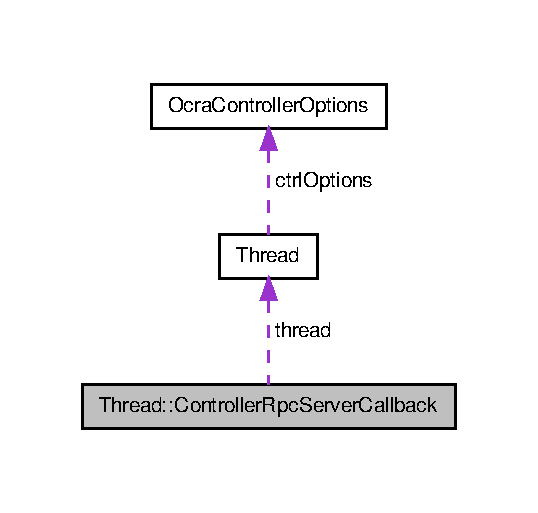
\includegraphics[width=258pt]{classThread_1_1ControllerRpcServerCallback__coll__graph}
\end{center}
\end{figure}
\subsection*{\-Public \-Member \-Functions}
\begin{DoxyCompactItemize}
\item 
\hyperlink{classThread_1_1ControllerRpcServerCallback_ad836e4cdaafc42ad309b5248ef38c280}{\-Controller\-Rpc\-Server\-Callback} (\hyperlink{classThread}{\-Thread} \&thread\-Ref)
\item 
virtual bool \hyperlink{classThread_1_1ControllerRpcServerCallback_a61f5510543f1bb96793dceca13eb6865}{read} (yarp\-::os\-::\-Connection\-Reader \&connection)
\end{DoxyCompactItemize}
\subsection*{\-Private \-Attributes}
\begin{DoxyCompactItemize}
\item 
\hyperlink{classThread}{\-Thread} \& \hyperlink{classThread_1_1ControllerRpcServerCallback_a466f100742fdac49e0016ec2f0c43536}{thread}
\end{DoxyCompactItemize}


\subsection{\-Detailed \-Description}
\-A callback function which binds the rpc server port opened in the contoller server module to the controller thread's parsing function. 

\subsection{\-Constructor \& \-Destructor \-Documentation}
\hypertarget{classThread_1_1ControllerRpcServerCallback_ad836e4cdaafc42ad309b5248ef38c280}{\index{\-Thread\-::\-Controller\-Rpc\-Server\-Callback@{\-Thread\-::\-Controller\-Rpc\-Server\-Callback}!\-Controller\-Rpc\-Server\-Callback@{\-Controller\-Rpc\-Server\-Callback}}
\index{\-Controller\-Rpc\-Server\-Callback@{\-Controller\-Rpc\-Server\-Callback}!Thread::ControllerRpcServerCallback@{\-Thread\-::\-Controller\-Rpc\-Server\-Callback}}
\subsubsection[{\-Controller\-Rpc\-Server\-Callback}]{\setlength{\rightskip}{0pt plus 5cm}{\bf \-Thread\-::\-Controller\-Rpc\-Server\-Callback\-::\-Controller\-Rpc\-Server\-Callback} (
\begin{DoxyParamCaption}
\item[{{\bf \-Thread} \&}]{thread\-Ref}
\end{DoxyParamCaption}
)}}\label{classThread_1_1ControllerRpcServerCallback_ad836e4cdaafc42ad309b5248ef38c280}
\-Constructor 
\begin{DoxyParams}{\-Parameters}
{\em ct\-Thread\-Ptr} & \-A shared pointer to the control thread. \\
\hline
\end{DoxyParams}


\subsection{\-Member \-Function \-Documentation}
\hypertarget{classThread_1_1ControllerRpcServerCallback_a61f5510543f1bb96793dceca13eb6865}{\index{\-Thread\-::\-Controller\-Rpc\-Server\-Callback@{\-Thread\-::\-Controller\-Rpc\-Server\-Callback}!read@{read}}
\index{read@{read}!Thread::ControllerRpcServerCallback@{\-Thread\-::\-Controller\-Rpc\-Server\-Callback}}
\subsubsection[{read}]{\setlength{\rightskip}{0pt plus 5cm}bool {\bf \-Thread\-::\-Controller\-Rpc\-Server\-Callback\-::read} (
\begin{DoxyParamCaption}
\item[{yarp\-::os\-::\-Connection\-Reader \&}]{connection}
\end{DoxyParamCaption}
)\hspace{0.3cm}{\ttfamily  \mbox{[}virtual\mbox{]}}}}\label{classThread_1_1ControllerRpcServerCallback_a61f5510543f1bb96793dceca13eb6865}
read 
\begin{DoxyParams}{\-Parameters}
{\em connection} & \-Reads a port connection.\\
\hline
\end{DoxyParams}
\begin{DoxyReturn}{\-Returns}
\-A boolean which tells whether or not a message was read. 
\end{DoxyReturn}


\subsection{\-Member \-Data \-Documentation}
\hypertarget{classThread_1_1ControllerRpcServerCallback_a466f100742fdac49e0016ec2f0c43536}{\index{\-Thread\-::\-Controller\-Rpc\-Server\-Callback@{\-Thread\-::\-Controller\-Rpc\-Server\-Callback}!thread@{thread}}
\index{thread@{thread}!Thread::ControllerRpcServerCallback@{\-Thread\-::\-Controller\-Rpc\-Server\-Callback}}
\subsubsection[{thread}]{\setlength{\rightskip}{0pt plus 5cm}{\bf \-Thread}\& {\bf \-Thread\-::\-Controller\-Rpc\-Server\-Callback\-::thread}\hspace{0.3cm}{\ttfamily  \mbox{[}private\mbox{]}}}}\label{classThread_1_1ControllerRpcServerCallback_a466f100742fdac49e0016ec2f0c43536}
\-A shared pointer to the control thread. 

\-The documentation for this class was generated from the following files\-:\begin{DoxyCompactItemize}
\item 
ocra-\/wbi-\/plugins/ocra-\/icub-\/server/include/ocra-\/icub-\/server/\hyperlink{Thread_8h}{\-Thread.\-h}\item 
ocra-\/wbi-\/plugins/ocra-\/icub-\/server/src/\hyperlink{Thread_8cpp}{\-Thread.\-cpp}\end{DoxyCompactItemize}

\hypertarget{classThread_1_1DebugRpcServerCallback}{\section{\-Thread\-:\-:\-Debug\-Rpc\-Server\-Callback \-Class \-Reference}
\label{classThread_1_1DebugRpcServerCallback}\index{\-Thread\-::\-Debug\-Rpc\-Server\-Callback@{\-Thread\-::\-Debug\-Rpc\-Server\-Callback}}
}


\-A callback function which binds the rpc server port opened in the contoller server module to the controller thread's parsing function.  




{\ttfamily \#include $<$\-Thread.\-h$>$}



\-Collaboration diagram for \-Thread\-:\-:\-Debug\-Rpc\-Server\-Callback\-:\nopagebreak
\begin{figure}[H]
\begin{center}
\leavevmode
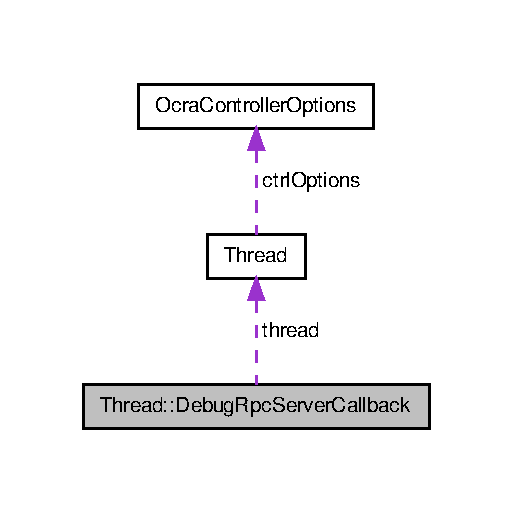
\includegraphics[width=246pt]{classThread_1_1DebugRpcServerCallback__coll__graph}
\end{center}
\end{figure}
\subsection*{\-Public \-Member \-Functions}
\begin{DoxyCompactItemize}
\item 
\hyperlink{classThread_1_1DebugRpcServerCallback_a479142cdf2f840df23b4605a532aaddf}{\-Debug\-Rpc\-Server\-Callback} (\hyperlink{classThread}{\-Thread} \&thread\-Ref)
\item 
virtual bool \hyperlink{classThread_1_1DebugRpcServerCallback_a3b39ac9b379ce3212bb2b05a89fa6024}{read} (yarp\-::os\-::\-Connection\-Reader \&connection)
\end{DoxyCompactItemize}
\subsection*{\-Private \-Attributes}
\begin{DoxyCompactItemize}
\item 
\hyperlink{classThread}{\-Thread} \& \hyperlink{classThread_1_1DebugRpcServerCallback_ad75683fc200019e8f681ad441b6ce84b}{thread}
\end{DoxyCompactItemize}


\subsection{\-Detailed \-Description}
\-A callback function which binds the rpc server port opened in the contoller server module to the controller thread's parsing function. 

\subsection{\-Constructor \& \-Destructor \-Documentation}
\hypertarget{classThread_1_1DebugRpcServerCallback_a479142cdf2f840df23b4605a532aaddf}{\index{\-Thread\-::\-Debug\-Rpc\-Server\-Callback@{\-Thread\-::\-Debug\-Rpc\-Server\-Callback}!\-Debug\-Rpc\-Server\-Callback@{\-Debug\-Rpc\-Server\-Callback}}
\index{\-Debug\-Rpc\-Server\-Callback@{\-Debug\-Rpc\-Server\-Callback}!Thread::DebugRpcServerCallback@{\-Thread\-::\-Debug\-Rpc\-Server\-Callback}}
\subsubsection[{\-Debug\-Rpc\-Server\-Callback}]{\setlength{\rightskip}{0pt plus 5cm}{\bf \-Thread\-::\-Debug\-Rpc\-Server\-Callback\-::\-Debug\-Rpc\-Server\-Callback} (
\begin{DoxyParamCaption}
\item[{{\bf \-Thread} \&}]{thread\-Ref}
\end{DoxyParamCaption}
)}}\label{classThread_1_1DebugRpcServerCallback_a479142cdf2f840df23b4605a532aaddf}
\-Constructor 
\begin{DoxyParams}{\-Parameters}
{\em ct\-Thread\-Ptr} & \-A shared pointer to the control thread. \\
\hline
\end{DoxyParams}


\subsection{\-Member \-Function \-Documentation}
\hypertarget{classThread_1_1DebugRpcServerCallback_a3b39ac9b379ce3212bb2b05a89fa6024}{\index{\-Thread\-::\-Debug\-Rpc\-Server\-Callback@{\-Thread\-::\-Debug\-Rpc\-Server\-Callback}!read@{read}}
\index{read@{read}!Thread::DebugRpcServerCallback@{\-Thread\-::\-Debug\-Rpc\-Server\-Callback}}
\subsubsection[{read}]{\setlength{\rightskip}{0pt plus 5cm}bool {\bf \-Thread\-::\-Debug\-Rpc\-Server\-Callback\-::read} (
\begin{DoxyParamCaption}
\item[{yarp\-::os\-::\-Connection\-Reader \&}]{connection}
\end{DoxyParamCaption}
)\hspace{0.3cm}{\ttfamily  \mbox{[}virtual\mbox{]}}}}\label{classThread_1_1DebugRpcServerCallback_a3b39ac9b379ce3212bb2b05a89fa6024}
read 
\begin{DoxyParams}{\-Parameters}
{\em connection} & \-Reads a port connection.\\
\hline
\end{DoxyParams}
\begin{DoxyReturn}{\-Returns}
\-A boolean which tells whether or not a message was read. 
\end{DoxyReturn}


\subsection{\-Member \-Data \-Documentation}
\hypertarget{classThread_1_1DebugRpcServerCallback_ad75683fc200019e8f681ad441b6ce84b}{\index{\-Thread\-::\-Debug\-Rpc\-Server\-Callback@{\-Thread\-::\-Debug\-Rpc\-Server\-Callback}!thread@{thread}}
\index{thread@{thread}!Thread::DebugRpcServerCallback@{\-Thread\-::\-Debug\-Rpc\-Server\-Callback}}
\subsubsection[{thread}]{\setlength{\rightskip}{0pt plus 5cm}{\bf \-Thread}\& {\bf \-Thread\-::\-Debug\-Rpc\-Server\-Callback\-::thread}\hspace{0.3cm}{\ttfamily  \mbox{[}private\mbox{]}}}}\label{classThread_1_1DebugRpcServerCallback_ad75683fc200019e8f681ad441b6ce84b}
\-A shared pointer to the control thread. 

\-The documentation for this class was generated from the following files\-:\begin{DoxyCompactItemize}
\item 
ocra-\/wbi-\/plugins/ocra-\/icub-\/server/include/ocra-\/icub-\/server/\hyperlink{Thread_8h}{\-Thread.\-h}\item 
ocra-\/wbi-\/plugins/ocra-\/icub-\/server/src/\hyperlink{Thread_8cpp}{\-Thread.\-cpp}\end{DoxyCompactItemize}

\hypertarget{classExampleClient}{\section{\-Example\-Client \-Class \-Reference}
\label{classExampleClient}\index{\-Example\-Client@{\-Example\-Client}}
}


{\ttfamily \#include $<$\-Example\-Client.\-h$>$}

\subsection*{\-Public \-Member \-Functions}
\begin{DoxyCompactItemize}
\item 
\hyperlink{classExampleClient_aed7d851662cba1484ecf1db8161d6e62}{\-Example\-Client} (std\-::shared\-\_\-ptr$<$ ocra\-::\-Model $>$ model\-Ptr, const int loop\-Period)
\item 
virtual \hyperlink{classExampleClient_abdca7dbe5fdab81d7d661a677e5ccd14}{$\sim$\-Example\-Client} ()
\end{DoxyCompactItemize}
\subsection*{\-Protected \-Member \-Functions}
\begin{DoxyCompactItemize}
\item 
virtual bool \hyperlink{classExampleClient_ad504d1d87997fc95bfeca6aa925a4fa6}{initialize} ()
\item 
virtual void \hyperlink{classExampleClient_a5acf25784c1c5b51c2c085327f195002}{release} ()
\item 
virtual void \hyperlink{classExampleClient_afb58f3425aafe2d4c38195cb3c667dbc}{loop} ()
\end{DoxyCompactItemize}
\subsection*{\-Private \-Attributes}
\begin{DoxyCompactItemize}
\item 
double \hyperlink{classExampleClient_aaa5ec782e9aaa1e94d7182872f743c02}{start\-Time}
\item 
double \hyperlink{classExampleClient_acade7035d4e39290cbda08b98249a629}{wait\-Time}
\item 
bool \hyperlink{classExampleClient_a90ce0c4d970c903b3e6afb6f5ca2a228}{trigger}
\item 
bool \hyperlink{classExampleClient_acd2cf0f0479ff8bbf5b64924d83beb60}{done}
\item 
\-Eigen\-::\-Matrix\-Xd \hyperlink{classExampleClient_acf4657277ecb08168d9a17c208814823}{waypoints}
\item 
std\-::shared\-\_\-ptr\*
$<$ ocra\-\_\-recipes\-::\-Trajectory\-Thread $>$ \hyperlink{classExampleClient_a4311b0e8c4878c23df2b5ba048d8bc05}{left\-Hand\-Traj\-Thread}
\item 
bool \hyperlink{classExampleClient_a7fb2b50cbdac0ec3a32e44b5bbc3b11f}{p1}
\item 
bool \hyperlink{classExampleClient_a07c2bc5c5c522e77a726017c28db2ec9}{p2}
\item 
bool \hyperlink{classExampleClient_ab41df6f34a51e649051adbac6d3077f9}{p3}
\end{DoxyCompactItemize}


\subsection{\-Constructor \& \-Destructor \-Documentation}
\hypertarget{classExampleClient_aed7d851662cba1484ecf1db8161d6e62}{\index{\-Example\-Client@{\-Example\-Client}!\-Example\-Client@{\-Example\-Client}}
\index{\-Example\-Client@{\-Example\-Client}!ExampleClient@{\-Example\-Client}}
\subsubsection[{\-Example\-Client}]{\setlength{\rightskip}{0pt plus 5cm}{\bf \-Example\-Client\-::\-Example\-Client} (
\begin{DoxyParamCaption}
\item[{std\-::shared\-\_\-ptr$<$ ocra\-::\-Model $>$}]{model\-Ptr, }
\item[{const int}]{loop\-Period}
\end{DoxyParamCaption}
)}}\label{classExampleClient_aed7d851662cba1484ecf1db8161d6e62}
\hypertarget{classExampleClient_abdca7dbe5fdab81d7d661a677e5ccd14}{\index{\-Example\-Client@{\-Example\-Client}!$\sim$\-Example\-Client@{$\sim$\-Example\-Client}}
\index{$\sim$\-Example\-Client@{$\sim$\-Example\-Client}!ExampleClient@{\-Example\-Client}}
\subsubsection[{$\sim$\-Example\-Client}]{\setlength{\rightskip}{0pt plus 5cm}{\bf \-Example\-Client\-::$\sim$\-Example\-Client} (
\begin{DoxyParamCaption}
{}
\end{DoxyParamCaption}
)\hspace{0.3cm}{\ttfamily  \mbox{[}virtual\mbox{]}}}}\label{classExampleClient_abdca7dbe5fdab81d7d661a677e5ccd14}


\subsection{\-Member \-Function \-Documentation}
\hypertarget{classExampleClient_ad504d1d87997fc95bfeca6aa925a4fa6}{\index{\-Example\-Client@{\-Example\-Client}!initialize@{initialize}}
\index{initialize@{initialize}!ExampleClient@{\-Example\-Client}}
\subsubsection[{initialize}]{\setlength{\rightskip}{0pt plus 5cm}bool {\bf \-Example\-Client\-::initialize} (
\begin{DoxyParamCaption}
{}
\end{DoxyParamCaption}
)\hspace{0.3cm}{\ttfamily  \mbox{[}protected, virtual\mbox{]}}}}\label{classExampleClient_ad504d1d87997fc95bfeca6aa925a4fa6}
\hypertarget{classExampleClient_afb58f3425aafe2d4c38195cb3c667dbc}{\index{\-Example\-Client@{\-Example\-Client}!loop@{loop}}
\index{loop@{loop}!ExampleClient@{\-Example\-Client}}
\subsubsection[{loop}]{\setlength{\rightskip}{0pt plus 5cm}void {\bf \-Example\-Client\-::loop} (
\begin{DoxyParamCaption}
{}
\end{DoxyParamCaption}
)\hspace{0.3cm}{\ttfamily  \mbox{[}protected, virtual\mbox{]}}}}\label{classExampleClient_afb58f3425aafe2d4c38195cb3c667dbc}
\hypertarget{classExampleClient_a5acf25784c1c5b51c2c085327f195002}{\index{\-Example\-Client@{\-Example\-Client}!release@{release}}
\index{release@{release}!ExampleClient@{\-Example\-Client}}
\subsubsection[{release}]{\setlength{\rightskip}{0pt plus 5cm}void {\bf \-Example\-Client\-::release} (
\begin{DoxyParamCaption}
{}
\end{DoxyParamCaption}
)\hspace{0.3cm}{\ttfamily  \mbox{[}protected, virtual\mbox{]}}}}\label{classExampleClient_a5acf25784c1c5b51c2c085327f195002}


\subsection{\-Member \-Data \-Documentation}
\hypertarget{classExampleClient_acd2cf0f0479ff8bbf5b64924d83beb60}{\index{\-Example\-Client@{\-Example\-Client}!done@{done}}
\index{done@{done}!ExampleClient@{\-Example\-Client}}
\subsubsection[{done}]{\setlength{\rightskip}{0pt plus 5cm}bool {\bf \-Example\-Client\-::done}\hspace{0.3cm}{\ttfamily  \mbox{[}private\mbox{]}}}}\label{classExampleClient_acd2cf0f0479ff8bbf5b64924d83beb60}
\hypertarget{classExampleClient_a4311b0e8c4878c23df2b5ba048d8bc05}{\index{\-Example\-Client@{\-Example\-Client}!left\-Hand\-Traj\-Thread@{left\-Hand\-Traj\-Thread}}
\index{left\-Hand\-Traj\-Thread@{left\-Hand\-Traj\-Thread}!ExampleClient@{\-Example\-Client}}
\subsubsection[{left\-Hand\-Traj\-Thread}]{\setlength{\rightskip}{0pt plus 5cm}std\-::shared\-\_\-ptr$<$ocra\-\_\-recipes\-::\-Trajectory\-Thread$>$ {\bf \-Example\-Client\-::left\-Hand\-Traj\-Thread}\hspace{0.3cm}{\ttfamily  \mbox{[}private\mbox{]}}}}\label{classExampleClient_a4311b0e8c4878c23df2b5ba048d8bc05}
\hypertarget{classExampleClient_a7fb2b50cbdac0ec3a32e44b5bbc3b11f}{\index{\-Example\-Client@{\-Example\-Client}!p1@{p1}}
\index{p1@{p1}!ExampleClient@{\-Example\-Client}}
\subsubsection[{p1}]{\setlength{\rightskip}{0pt plus 5cm}bool {\bf \-Example\-Client\-::p1}\hspace{0.3cm}{\ttfamily  \mbox{[}private\mbox{]}}}}\label{classExampleClient_a7fb2b50cbdac0ec3a32e44b5bbc3b11f}
\hypertarget{classExampleClient_a07c2bc5c5c522e77a726017c28db2ec9}{\index{\-Example\-Client@{\-Example\-Client}!p2@{p2}}
\index{p2@{p2}!ExampleClient@{\-Example\-Client}}
\subsubsection[{p2}]{\setlength{\rightskip}{0pt plus 5cm}bool {\bf \-Example\-Client\-::p2}\hspace{0.3cm}{\ttfamily  \mbox{[}private\mbox{]}}}}\label{classExampleClient_a07c2bc5c5c522e77a726017c28db2ec9}
\hypertarget{classExampleClient_ab41df6f34a51e649051adbac6d3077f9}{\index{\-Example\-Client@{\-Example\-Client}!p3@{p3}}
\index{p3@{p3}!ExampleClient@{\-Example\-Client}}
\subsubsection[{p3}]{\setlength{\rightskip}{0pt plus 5cm}bool {\bf \-Example\-Client\-::p3}\hspace{0.3cm}{\ttfamily  \mbox{[}private\mbox{]}}}}\label{classExampleClient_ab41df6f34a51e649051adbac6d3077f9}
\hypertarget{classExampleClient_aaa5ec782e9aaa1e94d7182872f743c02}{\index{\-Example\-Client@{\-Example\-Client}!start\-Time@{start\-Time}}
\index{start\-Time@{start\-Time}!ExampleClient@{\-Example\-Client}}
\subsubsection[{start\-Time}]{\setlength{\rightskip}{0pt plus 5cm}double {\bf \-Example\-Client\-::start\-Time}\hspace{0.3cm}{\ttfamily  \mbox{[}private\mbox{]}}}}\label{classExampleClient_aaa5ec782e9aaa1e94d7182872f743c02}
\hypertarget{classExampleClient_a90ce0c4d970c903b3e6afb6f5ca2a228}{\index{\-Example\-Client@{\-Example\-Client}!trigger@{trigger}}
\index{trigger@{trigger}!ExampleClient@{\-Example\-Client}}
\subsubsection[{trigger}]{\setlength{\rightskip}{0pt plus 5cm}bool {\bf \-Example\-Client\-::trigger}\hspace{0.3cm}{\ttfamily  \mbox{[}private\mbox{]}}}}\label{classExampleClient_a90ce0c4d970c903b3e6afb6f5ca2a228}
\hypertarget{classExampleClient_acade7035d4e39290cbda08b98249a629}{\index{\-Example\-Client@{\-Example\-Client}!wait\-Time@{wait\-Time}}
\index{wait\-Time@{wait\-Time}!ExampleClient@{\-Example\-Client}}
\subsubsection[{wait\-Time}]{\setlength{\rightskip}{0pt plus 5cm}double {\bf \-Example\-Client\-::wait\-Time}\hspace{0.3cm}{\ttfamily  \mbox{[}private\mbox{]}}}}\label{classExampleClient_acade7035d4e39290cbda08b98249a629}
\hypertarget{classExampleClient_acf4657277ecb08168d9a17c208814823}{\index{\-Example\-Client@{\-Example\-Client}!waypoints@{waypoints}}
\index{waypoints@{waypoints}!ExampleClient@{\-Example\-Client}}
\subsubsection[{waypoints}]{\setlength{\rightskip}{0pt plus 5cm}\-Eigen\-::\-Matrix\-Xd {\bf \-Example\-Client\-::waypoints}\hspace{0.3cm}{\ttfamily  \mbox{[}private\mbox{]}}}}\label{classExampleClient_acf4657277ecb08168d9a17c208814823}


\-The documentation for this class was generated from the following files\-:\begin{DoxyCompactItemize}
\item 
ocra-\/wbi-\/plugins/ocra-\/icub-\/clients/example-\/client/include/example-\/client/\hyperlink{ExampleClient_8h}{\-Example\-Client.\-h}\item 
ocra-\/wbi-\/plugins/ocra-\/icub-\/clients/example-\/client/src/\hyperlink{ExampleClient_8cpp}{\-Example\-Client.\-cpp}\end{DoxyCompactItemize}

\hypertarget{classIcubControllerServer}{\section{\-Icub\-Controller\-Server \-Class \-Reference}
\label{classIcubControllerServer}\index{\-Icub\-Controller\-Server@{\-Icub\-Controller\-Server}}
}


{\ttfamily \#include $<$\-Icub\-Controller\-Server.\-h$>$}

\subsection*{\-Public \-Member \-Functions}
\begin{DoxyCompactItemize}
\item 
\hyperlink{classIcubControllerServer_a6b0a6021e3c82e72ac97ad30d3f0c082}{\-Icub\-Controller\-Server} (std\-::shared\-\_\-ptr$<$ wbi\-::whole\-Body\-Interface $>$ robot, std\-::string icub\-Name, const bool using\-Floating\-Base, const ocra\-\_\-recipes\-::\-C\-O\-N\-T\-R\-O\-L\-L\-E\-R\-\_\-\-T\-Y\-P\-E ctrl\-Type=ocra\-\_\-recipes\-::\-W\-O\-C\-R\-A\-\_\-\-C\-O\-N\-T\-R\-O\-L\-L\-E\-R, const ocra\-\_\-recipes\-::\-S\-O\-L\-V\-E\-R\-\_\-\-T\-Y\-P\-E solver=ocra\-\_\-recipes\-::\-Q\-U\-A\-D\-P\-R\-O\-G, const bool using\-Interprocess\-Communication=true, const bool \hyperlink{classIcubControllerServer_adc410f503b14ed288c01e877ac405114}{use\-Odometry}=false)
\item 
virtual \hyperlink{classIcubControllerServer_a7582d4bbf9851ee9b58913ea2a89e5fd}{$\sim$\-Icub\-Controller\-Server} ()
\item 
virtual ocra\-::\-Model\-::\-Ptr \hyperlink{classIcubControllerServer_a025d8e257a69ef3d2c5a10b3cbfe2350}{load\-Robot\-Model} ()
\item 
virtual void \hyperlink{classIcubControllerServer_ac068c7930f342bb0cb0969d0d04267cf}{get\-Robot\-State} (\-Eigen\-::\-Vector\-Xd \&q, \-Eigen\-::\-Vector\-Xd \&qd, \-Eigen\-::\-Displacementd \&\-H\-\_\-root, \-Eigen\-::\-Twistd \&\-T\-\_\-root)
\item 
bool \hyperlink{classIcubControllerServer_a810f139a27e06458549ccbb3fde12359}{initialize\-Odometry} (std\-::string model\-\_\-file, std\-::string initial\-Fixed\-Frame)
\item 
std\-::vector$<$ std\-::string $>$ \hyperlink{classIcubControllerServer_a892bb43e568d3f112465dff1e0c6b348}{get\-Canonical\-\_\-i\-Cub\-Joints} ()
\item 
void \hyperlink{classIcubControllerServer_a032c035880f8ec2b77ef14521be6e75a}{root\-Frame\-Velocity} (\-Eigen\-::\-Vector\-Xd \&q, \-Eigen\-::\-Vector\-Xd \&qd, i\-Dyn\-Tree\-::\-Transform \&wbi\-\_\-\-H\-\_\-root\-\_\-\-Transform, double regularization, int \-L\-E\-F\-T\-\_\-\-F\-O\-O\-T\-\_\-\-C\-O\-N\-T\-A\-C\-T, int \-R\-I\-G\-H\-T\-\_\-\-F\-O\-O\-T\-\_\-\-C\-O\-N\-T\-A\-C\-T, \-Eigen\-::\-Vector\-Xd \&twist)
\item 
void \hyperlink{classIcubControllerServer_a27211ecba9fc8618733bcaea9ff7d140}{root\-Frame\-Velocity\-Piv\-L\-U} (\-Eigen\-::\-Vector\-Xd \&q, \-Eigen\-::\-Vector\-Xd \&qd, i\-Dyn\-Tree\-::\-Transform \&wbi\-\_\-\-H\-\_\-root\-\_\-\-Transform, \-Eigen\-::\-Vector\-Xd \&twist)
\item 
void \hyperlink{classIcubControllerServer_a82650f373c3c2c52a91cc744c67b0dcf}{root\-Frame\-Velocity\-Piv\-L\-U} (\-Eigen\-::\-Vector\-Xd \&q, \-Eigen\-::\-Vector\-Xd \&qd, i\-Dyn\-Tree\-::\-Transform \&wbi\-\_\-\-H\-\_\-root\-\_\-\-Transform, int \-L\-E\-F\-T\-\_\-\-F\-O\-O\-T\-\_\-\-C\-O\-N\-T\-A\-C\-T, int \-R\-I\-G\-H\-T\-\_\-\-F\-O\-O\-T\-\_\-\-C\-O\-N\-T\-A\-C\-T, \-Eigen\-::\-Vector\-Xd \&twist)
\item 
void \hyperlink{classIcubControllerServer_a0132b1ddc3dafd29506e4684ea42cf58}{pinv} (\-Eigen\-::\-Matrix\-Xd mat, \-Eigen\-::\-Matrix\-Xd \&pinvmat, double pinvtoler=1.\-0e-\/6) const 
\item 
void \hyperlink{classIcubControllerServer_aaedff28c5d9ac9a7cdbc24c9e0cbc5b3}{velocity\-Error} (\-Eigen\-::\-Matrix\-Xd \-A, \-Eigen\-::\-Matrix\-Xd \-B, \-Eigen\-::\-Matrix\-Xd \-X)
\end{DoxyCompactItemize}
\subsection*{\-Private \-Attributes}
\begin{DoxyCompactItemize}
\item 
std\-::shared\-\_\-ptr\*
$<$ wbi\-::whole\-Body\-Interface $>$ \hyperlink{classIcubControllerServer_ae8a89707675adb58bb3006bc085828b7}{wbi}
\item 
std\-::string \hyperlink{classIcubControllerServer_a041d6687258c36677914b1d15f18e153}{robot\-Name}
\item 
bool \hyperlink{classIcubControllerServer_aebc2019921c3eabb53c01012fbd2355a}{is\-Floating\-Base}
\item 
bool \hyperlink{classIcubControllerServer_adc410f503b14ed288c01e877ac405114}{use\-Odometry}
\item 
int \hyperlink{classIcubControllerServer_ab5fb1f18775cfe3036894c73dc21ebcf}{n\-Do\-F}
\item 
\-Eigen\-::\-Vector\-Xd \hyperlink{classIcubControllerServer_a42f6a8db660da9dbafbc57941b1ee12f}{wbi\-\_\-\-H\-\_\-root\-\_\-\-Vector}
\item 
\-Eigen\-::\-Vector\-Xd \hyperlink{classIcubControllerServer_a818b66e75b7f9457a6a5bcbb3c1306a7}{wbi\-\_\-\-T\-\_\-root\-\_\-\-Vector}
\item 
wbi\-::\-Frame \hyperlink{classIcubControllerServer_afd983b69c043eedf958e53582b22195a}{wbi\-\_\-\-H\-\_\-root}
\item 
i\-Dyn\-Tree\-::\-Simple\-Legged\-Odometry \hyperlink{classIcubControllerServer_ad0484106ab9d7fd42e2bd682338871c7}{odometry}
\end{DoxyCompactItemize}
\subsection*{\-Static \-Private \-Attributes}
\begin{DoxyCompactItemize}
\item 
static const int \hyperlink{classIcubControllerServer_aa977ca558c184e4331121522cc58d2e7}{\-A\-L\-L\-\_\-\-J\-O\-I\-N\-T\-S} = -\/1
\end{DoxyCompactItemize}


\subsection{\-Constructor \& \-Destructor \-Documentation}
\hypertarget{classIcubControllerServer_a6b0a6021e3c82e72ac97ad30d3f0c082}{\index{\-Icub\-Controller\-Server@{\-Icub\-Controller\-Server}!\-Icub\-Controller\-Server@{\-Icub\-Controller\-Server}}
\index{\-Icub\-Controller\-Server@{\-Icub\-Controller\-Server}!IcubControllerServer@{\-Icub\-Controller\-Server}}
\subsubsection[{\-Icub\-Controller\-Server}]{\setlength{\rightskip}{0pt plus 5cm}{\bf \-Icub\-Controller\-Server\-::\-Icub\-Controller\-Server} (
\begin{DoxyParamCaption}
\item[{std\-::shared\-\_\-ptr$<$ wbi\-::whole\-Body\-Interface $>$}]{robot, }
\item[{std\-::string}]{icub\-Name, }
\item[{const bool}]{using\-Floating\-Base, }
\item[{const ocra\-\_\-recipes\-::\-C\-O\-N\-T\-R\-O\-L\-L\-E\-R\-\_\-\-T\-Y\-P\-E}]{ctrl\-Type = {\ttfamily ocra\-\_\-recipes\-:\-:\-W\-O\-C\-R\-A\-\_\-\-C\-O\-N\-T\-R\-O\-L\-L\-E\-R}, }
\item[{const ocra\-\_\-recipes\-::\-S\-O\-L\-V\-E\-R\-\_\-\-T\-Y\-P\-E}]{solver = {\ttfamily ocra\-\_\-recipes\-:\-:\-Q\-U\-A\-D\-P\-R\-O\-G}, }
\item[{const bool}]{using\-Interprocess\-Communication = {\ttfamily true}, }
\item[{const bool}]{use\-Odometry = {\ttfamily false}}
\end{DoxyParamCaption}
)}}\label{classIcubControllerServer_a6b0a6021e3c82e72ac97ad30d3f0c082}
\hypertarget{classIcubControllerServer_a7582d4bbf9851ee9b58913ea2a89e5fd}{\index{\-Icub\-Controller\-Server@{\-Icub\-Controller\-Server}!$\sim$\-Icub\-Controller\-Server@{$\sim$\-Icub\-Controller\-Server}}
\index{$\sim$\-Icub\-Controller\-Server@{$\sim$\-Icub\-Controller\-Server}!IcubControllerServer@{\-Icub\-Controller\-Server}}
\subsubsection[{$\sim$\-Icub\-Controller\-Server}]{\setlength{\rightskip}{0pt plus 5cm}{\bf \-Icub\-Controller\-Server\-::$\sim$\-Icub\-Controller\-Server} (
\begin{DoxyParamCaption}
{}
\end{DoxyParamCaption}
)\hspace{0.3cm}{\ttfamily  \mbox{[}virtual\mbox{]}}}}\label{classIcubControllerServer_a7582d4bbf9851ee9b58913ea2a89e5fd}


\subsection{\-Member \-Function \-Documentation}
\hypertarget{classIcubControllerServer_a892bb43e568d3f112465dff1e0c6b348}{\index{\-Icub\-Controller\-Server@{\-Icub\-Controller\-Server}!get\-Canonical\-\_\-i\-Cub\-Joints@{get\-Canonical\-\_\-i\-Cub\-Joints}}
\index{get\-Canonical\-\_\-i\-Cub\-Joints@{get\-Canonical\-\_\-i\-Cub\-Joints}!IcubControllerServer@{\-Icub\-Controller\-Server}}
\subsubsection[{get\-Canonical\-\_\-i\-Cub\-Joints}]{\setlength{\rightskip}{0pt plus 5cm}std\-::vector$<$ std\-::string $>$ {\bf \-Icub\-Controller\-Server\-::get\-Canonical\-\_\-i\-Cub\-Joints} (
\begin{DoxyParamCaption}
{}
\end{DoxyParamCaption}
)}}\label{classIcubControllerServer_a892bb43e568d3f112465dff1e0c6b348}
\hypertarget{classIcubControllerServer_ac068c7930f342bb0cb0969d0d04267cf}{\index{\-Icub\-Controller\-Server@{\-Icub\-Controller\-Server}!get\-Robot\-State@{get\-Robot\-State}}
\index{get\-Robot\-State@{get\-Robot\-State}!IcubControllerServer@{\-Icub\-Controller\-Server}}
\subsubsection[{get\-Robot\-State}]{\setlength{\rightskip}{0pt plus 5cm}void {\bf \-Icub\-Controller\-Server\-::get\-Robot\-State} (
\begin{DoxyParamCaption}
\item[{\-Eigen\-::\-Vector\-Xd \&}]{q, }
\item[{\-Eigen\-::\-Vector\-Xd \&}]{qd, }
\item[{\-Eigen\-::\-Displacementd \&}]{\-H\-\_\-root, }
\item[{\-Eigen\-::\-Twistd \&}]{\-T\-\_\-root}
\end{DoxyParamCaption}
)\hspace{0.3cm}{\ttfamily  \mbox{[}virtual\mbox{]}}}}\label{classIcubControllerServer_ac068c7930f342bb0cb0969d0d04267cf}
\hypertarget{classIcubControllerServer_a810f139a27e06458549ccbb3fde12359}{\index{\-Icub\-Controller\-Server@{\-Icub\-Controller\-Server}!initialize\-Odometry@{initialize\-Odometry}}
\index{initialize\-Odometry@{initialize\-Odometry}!IcubControllerServer@{\-Icub\-Controller\-Server}}
\subsubsection[{initialize\-Odometry}]{\setlength{\rightskip}{0pt plus 5cm}bool {\bf \-Icub\-Controller\-Server\-::initialize\-Odometry} (
\begin{DoxyParamCaption}
\item[{std\-::string}]{model\-\_\-file, }
\item[{std\-::string}]{initial\-Fixed\-Frame}
\end{DoxyParamCaption}
)}}\label{classIcubControllerServer_a810f139a27e06458549ccbb3fde12359}
\hypertarget{classIcubControllerServer_a025d8e257a69ef3d2c5a10b3cbfe2350}{\index{\-Icub\-Controller\-Server@{\-Icub\-Controller\-Server}!load\-Robot\-Model@{load\-Robot\-Model}}
\index{load\-Robot\-Model@{load\-Robot\-Model}!IcubControllerServer@{\-Icub\-Controller\-Server}}
\subsubsection[{load\-Robot\-Model}]{\setlength{\rightskip}{0pt plus 5cm}ocra\-::\-Model\-::\-Ptr {\bf \-Icub\-Controller\-Server\-::load\-Robot\-Model} (
\begin{DoxyParamCaption}
{}
\end{DoxyParamCaption}
)\hspace{0.3cm}{\ttfamily  \mbox{[}virtual\mbox{]}}}}\label{classIcubControllerServer_a025d8e257a69ef3d2c5a10b3cbfe2350}
\hypertarget{classIcubControllerServer_a0132b1ddc3dafd29506e4684ea42cf58}{\index{\-Icub\-Controller\-Server@{\-Icub\-Controller\-Server}!pinv@{pinv}}
\index{pinv@{pinv}!IcubControllerServer@{\-Icub\-Controller\-Server}}
\subsubsection[{pinv}]{\setlength{\rightskip}{0pt plus 5cm}void {\bf \-Icub\-Controller\-Server\-::pinv} (
\begin{DoxyParamCaption}
\item[{\-Eigen\-::\-Matrix\-Xd}]{mat, }
\item[{\-Eigen\-::\-Matrix\-Xd \&}]{pinvmat, }
\item[{double}]{pinvtoler = {\ttfamily 1.0e-\/6}}
\end{DoxyParamCaption}
) const}}\label{classIcubControllerServer_a0132b1ddc3dafd29506e4684ea42cf58}
\hypertarget{classIcubControllerServer_a032c035880f8ec2b77ef14521be6e75a}{\index{\-Icub\-Controller\-Server@{\-Icub\-Controller\-Server}!root\-Frame\-Velocity@{root\-Frame\-Velocity}}
\index{root\-Frame\-Velocity@{root\-Frame\-Velocity}!IcubControllerServer@{\-Icub\-Controller\-Server}}
\subsubsection[{root\-Frame\-Velocity}]{\setlength{\rightskip}{0pt plus 5cm}void {\bf \-Icub\-Controller\-Server\-::root\-Frame\-Velocity} (
\begin{DoxyParamCaption}
\item[{\-Eigen\-::\-Vector\-Xd \&}]{q, }
\item[{\-Eigen\-::\-Vector\-Xd \&}]{qd, }
\item[{i\-Dyn\-Tree\-::\-Transform \&}]{wbi\-\_\-\-H\-\_\-root\-\_\-\-Transform, }
\item[{double}]{regularization, }
\item[{int}]{\-L\-E\-F\-T\-\_\-\-F\-O\-O\-T\-\_\-\-C\-O\-N\-T\-A\-C\-T, }
\item[{int}]{\-R\-I\-G\-H\-T\-\_\-\-F\-O\-O\-T\-\_\-\-C\-O\-N\-T\-A\-C\-T, }
\item[{\-Eigen\-::\-Vector\-Xd \&}]{twist}
\end{DoxyParamCaption}
)}}\label{classIcubControllerServer_a032c035880f8ec2b77ef14521be6e75a}
\hypertarget{classIcubControllerServer_a27211ecba9fc8618733bcaea9ff7d140}{\index{\-Icub\-Controller\-Server@{\-Icub\-Controller\-Server}!root\-Frame\-Velocity\-Piv\-L\-U@{root\-Frame\-Velocity\-Piv\-L\-U}}
\index{root\-Frame\-Velocity\-Piv\-L\-U@{root\-Frame\-Velocity\-Piv\-L\-U}!IcubControllerServer@{\-Icub\-Controller\-Server}}
\subsubsection[{root\-Frame\-Velocity\-Piv\-L\-U}]{\setlength{\rightskip}{0pt plus 5cm}void {\bf \-Icub\-Controller\-Server\-::root\-Frame\-Velocity\-Piv\-L\-U} (
\begin{DoxyParamCaption}
\item[{\-Eigen\-::\-Vector\-Xd \&}]{q, }
\item[{\-Eigen\-::\-Vector\-Xd \&}]{qd, }
\item[{i\-Dyn\-Tree\-::\-Transform \&}]{wbi\-\_\-\-H\-\_\-root\-\_\-\-Transform, }
\item[{\-Eigen\-::\-Vector\-Xd \&}]{twist}
\end{DoxyParamCaption}
)}}\label{classIcubControllerServer_a27211ecba9fc8618733bcaea9ff7d140}
\hypertarget{classIcubControllerServer_a82650f373c3c2c52a91cc744c67b0dcf}{\index{\-Icub\-Controller\-Server@{\-Icub\-Controller\-Server}!root\-Frame\-Velocity\-Piv\-L\-U@{root\-Frame\-Velocity\-Piv\-L\-U}}
\index{root\-Frame\-Velocity\-Piv\-L\-U@{root\-Frame\-Velocity\-Piv\-L\-U}!IcubControllerServer@{\-Icub\-Controller\-Server}}
\subsubsection[{root\-Frame\-Velocity\-Piv\-L\-U}]{\setlength{\rightskip}{0pt plus 5cm}void {\bf \-Icub\-Controller\-Server\-::root\-Frame\-Velocity\-Piv\-L\-U} (
\begin{DoxyParamCaption}
\item[{\-Eigen\-::\-Vector\-Xd \&}]{q, }
\item[{\-Eigen\-::\-Vector\-Xd \&}]{qd, }
\item[{i\-Dyn\-Tree\-::\-Transform \&}]{wbi\-\_\-\-H\-\_\-root\-\_\-\-Transform, }
\item[{int}]{\-L\-E\-F\-T\-\_\-\-F\-O\-O\-T\-\_\-\-C\-O\-N\-T\-A\-C\-T, }
\item[{int}]{\-R\-I\-G\-H\-T\-\_\-\-F\-O\-O\-T\-\_\-\-C\-O\-N\-T\-A\-C\-T, }
\item[{\-Eigen\-::\-Vector\-Xd \&}]{twist}
\end{DoxyParamCaption}
)}}\label{classIcubControllerServer_a82650f373c3c2c52a91cc744c67b0dcf}
\hypertarget{classIcubControllerServer_aaedff28c5d9ac9a7cdbc24c9e0cbc5b3}{\index{\-Icub\-Controller\-Server@{\-Icub\-Controller\-Server}!velocity\-Error@{velocity\-Error}}
\index{velocity\-Error@{velocity\-Error}!IcubControllerServer@{\-Icub\-Controller\-Server}}
\subsubsection[{velocity\-Error}]{\setlength{\rightskip}{0pt plus 5cm}void {\bf \-Icub\-Controller\-Server\-::velocity\-Error} (
\begin{DoxyParamCaption}
\item[{\-Eigen\-::\-Matrix\-Xd}]{\-A, }
\item[{\-Eigen\-::\-Matrix\-Xd}]{\-B, }
\item[{\-Eigen\-::\-Matrix\-Xd}]{\-X}
\end{DoxyParamCaption}
)}}\label{classIcubControllerServer_aaedff28c5d9ac9a7cdbc24c9e0cbc5b3}


\subsection{\-Member \-Data \-Documentation}
\hypertarget{classIcubControllerServer_aa977ca558c184e4331121522cc58d2e7}{\index{\-Icub\-Controller\-Server@{\-Icub\-Controller\-Server}!\-A\-L\-L\-\_\-\-J\-O\-I\-N\-T\-S@{\-A\-L\-L\-\_\-\-J\-O\-I\-N\-T\-S}}
\index{\-A\-L\-L\-\_\-\-J\-O\-I\-N\-T\-S@{\-A\-L\-L\-\_\-\-J\-O\-I\-N\-T\-S}!IcubControllerServer@{\-Icub\-Controller\-Server}}
\subsubsection[{\-A\-L\-L\-\_\-\-J\-O\-I\-N\-T\-S}]{\setlength{\rightskip}{0pt plus 5cm}const int {\bf \-Icub\-Controller\-Server\-::\-A\-L\-L\-\_\-\-J\-O\-I\-N\-T\-S} = -\/1\hspace{0.3cm}{\ttfamily  \mbox{[}static, private\mbox{]}}}}\label{classIcubControllerServer_aa977ca558c184e4331121522cc58d2e7}
\hypertarget{classIcubControllerServer_aebc2019921c3eabb53c01012fbd2355a}{\index{\-Icub\-Controller\-Server@{\-Icub\-Controller\-Server}!is\-Floating\-Base@{is\-Floating\-Base}}
\index{is\-Floating\-Base@{is\-Floating\-Base}!IcubControllerServer@{\-Icub\-Controller\-Server}}
\subsubsection[{is\-Floating\-Base}]{\setlength{\rightskip}{0pt plus 5cm}bool {\bf \-Icub\-Controller\-Server\-::is\-Floating\-Base}\hspace{0.3cm}{\ttfamily  \mbox{[}private\mbox{]}}}}\label{classIcubControllerServer_aebc2019921c3eabb53c01012fbd2355a}
\hypertarget{classIcubControllerServer_ab5fb1f18775cfe3036894c73dc21ebcf}{\index{\-Icub\-Controller\-Server@{\-Icub\-Controller\-Server}!n\-Do\-F@{n\-Do\-F}}
\index{n\-Do\-F@{n\-Do\-F}!IcubControllerServer@{\-Icub\-Controller\-Server}}
\subsubsection[{n\-Do\-F}]{\setlength{\rightskip}{0pt plus 5cm}int {\bf \-Icub\-Controller\-Server\-::n\-Do\-F}\hspace{0.3cm}{\ttfamily  \mbox{[}private\mbox{]}}}}\label{classIcubControllerServer_ab5fb1f18775cfe3036894c73dc21ebcf}
\hypertarget{classIcubControllerServer_ad0484106ab9d7fd42e2bd682338871c7}{\index{\-Icub\-Controller\-Server@{\-Icub\-Controller\-Server}!odometry@{odometry}}
\index{odometry@{odometry}!IcubControllerServer@{\-Icub\-Controller\-Server}}
\subsubsection[{odometry}]{\setlength{\rightskip}{0pt plus 5cm}i\-Dyn\-Tree\-::\-Simple\-Legged\-Odometry {\bf \-Icub\-Controller\-Server\-::odometry}\hspace{0.3cm}{\ttfamily  \mbox{[}private\mbox{]}}}}\label{classIcubControllerServer_ad0484106ab9d7fd42e2bd682338871c7}
\hypertarget{classIcubControllerServer_a041d6687258c36677914b1d15f18e153}{\index{\-Icub\-Controller\-Server@{\-Icub\-Controller\-Server}!robot\-Name@{robot\-Name}}
\index{robot\-Name@{robot\-Name}!IcubControllerServer@{\-Icub\-Controller\-Server}}
\subsubsection[{robot\-Name}]{\setlength{\rightskip}{0pt plus 5cm}std\-::string {\bf \-Icub\-Controller\-Server\-::robot\-Name}\hspace{0.3cm}{\ttfamily  \mbox{[}private\mbox{]}}}}\label{classIcubControllerServer_a041d6687258c36677914b1d15f18e153}
\hypertarget{classIcubControllerServer_adc410f503b14ed288c01e877ac405114}{\index{\-Icub\-Controller\-Server@{\-Icub\-Controller\-Server}!use\-Odometry@{use\-Odometry}}
\index{use\-Odometry@{use\-Odometry}!IcubControllerServer@{\-Icub\-Controller\-Server}}
\subsubsection[{use\-Odometry}]{\setlength{\rightskip}{0pt plus 5cm}bool {\bf \-Icub\-Controller\-Server\-::use\-Odometry}\hspace{0.3cm}{\ttfamily  \mbox{[}private\mbox{]}}}}\label{classIcubControllerServer_adc410f503b14ed288c01e877ac405114}
\hypertarget{classIcubControllerServer_ae8a89707675adb58bb3006bc085828b7}{\index{\-Icub\-Controller\-Server@{\-Icub\-Controller\-Server}!wbi@{wbi}}
\index{wbi@{wbi}!IcubControllerServer@{\-Icub\-Controller\-Server}}
\subsubsection[{wbi}]{\setlength{\rightskip}{0pt plus 5cm}std\-::shared\-\_\-ptr$<$wbi\-::whole\-Body\-Interface$>$ {\bf \-Icub\-Controller\-Server\-::wbi}\hspace{0.3cm}{\ttfamily  \mbox{[}private\mbox{]}}}}\label{classIcubControllerServer_ae8a89707675adb58bb3006bc085828b7}
\-The \-W\-B\-I used to talk to the robot. \hypertarget{classIcubControllerServer_afd983b69c043eedf958e53582b22195a}{\index{\-Icub\-Controller\-Server@{\-Icub\-Controller\-Server}!wbi\-\_\-\-H\-\_\-root@{wbi\-\_\-\-H\-\_\-root}}
\index{wbi\-\_\-\-H\-\_\-root@{wbi\-\_\-\-H\-\_\-root}!IcubControllerServer@{\-Icub\-Controller\-Server}}
\subsubsection[{wbi\-\_\-\-H\-\_\-root}]{\setlength{\rightskip}{0pt plus 5cm}wbi\-::\-Frame {\bf \-Icub\-Controller\-Server\-::wbi\-\_\-\-H\-\_\-root}\hspace{0.3cm}{\ttfamily  \mbox{[}private\mbox{]}}}}\label{classIcubControllerServer_afd983b69c043eedf958e53582b22195a}
\hypertarget{classIcubControllerServer_a42f6a8db660da9dbafbc57941b1ee12f}{\index{\-Icub\-Controller\-Server@{\-Icub\-Controller\-Server}!wbi\-\_\-\-H\-\_\-root\-\_\-\-Vector@{wbi\-\_\-\-H\-\_\-root\-\_\-\-Vector}}
\index{wbi\-\_\-\-H\-\_\-root\-\_\-\-Vector@{wbi\-\_\-\-H\-\_\-root\-\_\-\-Vector}!IcubControllerServer@{\-Icub\-Controller\-Server}}
\subsubsection[{wbi\-\_\-\-H\-\_\-root\-\_\-\-Vector}]{\setlength{\rightskip}{0pt plus 5cm}\-Eigen\-::\-Vector\-Xd {\bf \-Icub\-Controller\-Server\-::wbi\-\_\-\-H\-\_\-root\-\_\-\-Vector}\hspace{0.3cm}{\ttfamily  \mbox{[}private\mbox{]}}}}\label{classIcubControllerServer_a42f6a8db660da9dbafbc57941b1ee12f}
\hypertarget{classIcubControllerServer_a818b66e75b7f9457a6a5bcbb3c1306a7}{\index{\-Icub\-Controller\-Server@{\-Icub\-Controller\-Server}!wbi\-\_\-\-T\-\_\-root\-\_\-\-Vector@{wbi\-\_\-\-T\-\_\-root\-\_\-\-Vector}}
\index{wbi\-\_\-\-T\-\_\-root\-\_\-\-Vector@{wbi\-\_\-\-T\-\_\-root\-\_\-\-Vector}!IcubControllerServer@{\-Icub\-Controller\-Server}}
\subsubsection[{wbi\-\_\-\-T\-\_\-root\-\_\-\-Vector}]{\setlength{\rightskip}{0pt plus 5cm}\-Eigen\-::\-Vector\-Xd {\bf \-Icub\-Controller\-Server\-::wbi\-\_\-\-T\-\_\-root\-\_\-\-Vector}\hspace{0.3cm}{\ttfamily  \mbox{[}private\mbox{]}}}}\label{classIcubControllerServer_a818b66e75b7f9457a6a5bcbb3c1306a7}


\-The documentation for this class was generated from the following files\-:\begin{DoxyCompactItemize}
\item 
ocra-\/wbi-\/plugins/ocra-\/icub-\/server/include/ocra-\/icub-\/server/\hyperlink{IcubControllerServer_8h}{\-Icub\-Controller\-Server.\-h}\item 
ocra-\/wbi-\/plugins/ocra-\/icub-\/server/src/\hyperlink{IcubControllerServer_8cpp}{\-Icub\-Controller\-Server.\-cpp}\end{DoxyCompactItemize}

\hypertarget{classMIQPController}{\section{\-M\-I\-Q\-P\-Controller \-Class \-Reference}
\label{classMIQPController}\index{\-M\-I\-Q\-P\-Controller@{\-M\-I\-Q\-P\-Controller}}
}


{\ttfamily \#include $<$\-M\-I\-Q\-P\-Controller.\-h$>$}



\-Collaboration diagram for \-M\-I\-Q\-P\-Controller\-:\nopagebreak
\begin{figure}[H]
\begin{center}
\leavevmode
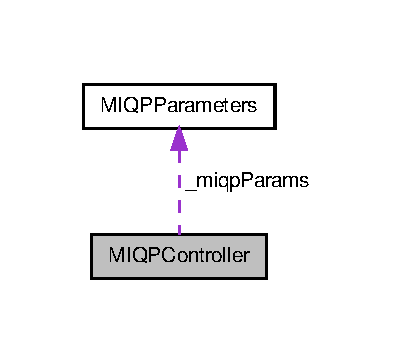
\includegraphics[width=190pt]{classMIQPController__coll__graph}
\end{center}
\end{figure}
\subsection*{\-Public \-Member \-Functions}
\begin{DoxyCompactItemize}
\item 
\hyperlink{classMIQPController_a5fec189a29105d999d3bb2721977945a}{\-M\-I\-Q\-P\-Controller} (\hyperlink{structMIQPParameters}{\-M\-I\-Q\-P\-Parameters} params, ocra\-::\-Model\-::\-Ptr robot\-Model, std\-::shared\-\_\-ptr$<$ \hyperlink{classStepController}{\-Step\-Controller} $>$ step\-Controller, const \-Eigen\-::\-Matrix\-Xd \&com\-State\-Ref)
\item 
virtual \hyperlink{classMIQPController_a46e1cc8dba1633a49d934aa20730e358}{$\sim$\-M\-I\-Q\-P\-Controller} ()
\item 
virtual bool \hyperlink{classMIQPController_a7e82a26dc823c7f69d00997d0ca98052}{thread\-Init} ()
\item 
virtual void \hyperlink{classMIQPController_a43faa045ed47859b04f39e99805888c1}{thread\-Release} ()
\item 
virtual void \hyperlink{classMIQPController_aa8fd8452a14d8e7731bf45044e1c7a59}{run} ()
\item 
void \hyperlink{classMIQPController_a69b193f0aab0fa0d0ec439b4d1b2a65f}{set\-C\-O\-M\-State\-Ref\-In\-Preview\-Window} (unsigned int k, \-Eigen\-::\-Vector\-Xd \&com\-State\-Ref)
\item 
void \hyperlink{classMIQPController_a96e30b0c6f47973ec1dd3cf745083f71}{get\-Solution} (\-Eigen\-::\-Vector\-Xd \&\-X\-\_\-kn)
\end{DoxyCompactItemize}
\subsection*{\-Public \-Attributes}
\begin{DoxyCompactItemize}
\item 
yarp\-::os\-::\-Semaphore \hyperlink{classMIQPController_ae9a603043a180264edabf45320d530ca}{semaphore}
\end{DoxyCompactItemize}
\subsection*{\-Protected \-Member \-Functions}
\begin{DoxyCompactItemize}
\item 
void \hyperlink{classMIQPController_a2d882a4cd9e9832d8b9b2ad73111be0f}{set\-Linear\-Part\-Objective\-Function} ()
\item 
void \hyperlink{classMIQPController_a2caf42a5b5dcd63d67de57cfbb93c653}{set\-Lower\-And\-Upper\-Bounds} ()
\item 
void \hyperlink{classMIQPController_a8320465a1ec80d0cf7ba0d17652feba5}{update\-State\-Vector} ()
\item 
void \hyperlink{classMIQPController_aea16b6eac86da5330c7ffbfdb9c655f5}{build\-Ah} (int dt, \-Eigen\-::\-Matrix\-Xd \&output)
\item 
void \hyperlink{classMIQPController_afc2df705b1238e2503e35f07e2f8270a}{build\-Bh} (int dt, \-Eigen\-::\-Matrix\-Xd \&output)
\item 
void \hyperlink{classMIQPController_af492dfbff2e211ff1c1351c2193fe669}{build\-Q} (\-Eigen\-::\-Matrix\-Xd \&output)
\item 
void \hyperlink{classMIQPController_a52dc10cbc0941a6e4f4e6ffd462fffce}{build\-T} (\-Eigen\-::\-Matrix\-Xd \&output)
\item 
void \hyperlink{classMIQPController_aa58686fc2883ef2d81d3e6d3554b338d}{build\-C\-\_\-\-H} (\-Eigen\-::\-Matrix\-Xd \&output)
\item 
void \hyperlink{classMIQPController_ac2a454e236bdb3a13b72b6930329f231}{build\-C\-\_\-\-P} (\-Eigen\-::\-Matrix\-Xd \&output)
\item 
void \hyperlink{classMIQPController_a1be33f8ebb313f7ecddd2aa6af4fa62c}{build\-C\-\_\-\-B} (\-Eigen\-::\-Matrix\-Xd \&output)
\item 
void \hyperlink{classMIQPController_ab093df4b1c73c02a97609093fd037345}{build\-H\-\_\-\-N} (\-Eigen\-::\-Matrix\-Xd \&output)
\item 
void \hyperlink{classMIQPController_a8b83fba21208a3becff314d26ba45679}{build\-Nb} (\-Eigen\-::\-Matrix\-Xd \&output, double wb)
\item 
void \hyperlink{classMIQPController_a959d9957a931315d3f1cf95ad5c07a65}{build\-Nx} (\-Eigen\-::\-Matrix\-Xd \&output)
\item 
void \hyperlink{classMIQPController_ab8b3555a9f64417f2b986784c3ab8bd6}{build\-Generic\-Reg\-Mat} (\hyperlink{namespaceMIQP_a88adf7c800494cf6d751d065e642b45b}{\-M\-I\-Q\-P\-::\-Input\-Vector\-Index} which\-Variable, double weight, \-Eigen\-::\-Matrix\-Xd \&output)
\item 
void \hyperlink{classMIQPController_a3085bba3c89e6ed0265e8e229590e7f1}{build\-Sw} (\-Eigen\-::\-Matrix\-Xd \&output, \hyperlink{structMIQPParameters}{\-M\-I\-Q\-P\-Parameters} miqp\-Params)
\item 
void \hyperlink{classMIQPController_ad9a2e7d2c658937c847097f83d3408e3}{build\-Preview\-State\-Matrix} (const \-Eigen\-::\-Matrix\-Xd \&\-C, \-Eigen\-::\-Matrix\-Xd \&\-P)
\item 
void \hyperlink{classMIQPController_a9e4f007d1b6b7f68582aebbc09cf0813}{build\-Preview\-Input\-Matrix} (const \-Eigen\-::\-Matrix\-Xd \&\-C, \-Eigen\-::\-Matrix\-Xd \&\-R)
\item 
void \hyperlink{classMIQPController_a870c7d3c0e5fcfd46f7bb95924007082}{build\-Equality\-Constraints\-Matrices} (const \-Eigen\-::\-Vector\-Xd \&x\-\_\-k, \-Eigen\-::\-Matrix\-Xd \&\-Aeq, \-Eigen\-::\-Vector\-Xd \&\-Beq)
\item 
void \hyperlink{classMIQPController_a4c3f665528fae6c051160456692372ee}{update\-Equality\-Constraints} (const \-Eigen\-::\-Vector\-Xd \&x\-\_\-k, \-Eigen\-::\-Vector\-Xd \&\-Beq)
\item 
void \hyperlink{classMIQPController_a973c28f80d04db7cdbdced07e1eeda16}{build\-Regularization\-Terms} (\hyperlink{structMIQPParameters}{\-M\-I\-Q\-P\-Parameters} \&miqp\-Params)
\item 
void \hyperlink{classMIQPController_ac458316007d11e4b592cfb2e227bad69}{build\-Co\-M\-Jerk\-Reg} (\hyperlink{structMIQPParameters}{\-M\-I\-Q\-P\-Parameters} \&miqp\-Params)
\item 
void \hyperlink{classMIQPController_ad18d82e49c5508dc0239c21a85809131}{build\-Avoid\-One\-Foot\-Rest\-Reg} (\hyperlink{structMIQPParameters}{\-M\-I\-Q\-P\-Parameters} \&miqp\-Params)
\item 
void \hyperlink{classMIQPController_af721e438de3208adc893abe78551a0cb}{build\-Minimize\-Stepping\-Reg} (\hyperlink{structMIQPParameters}{\-M\-I\-Q\-P\-Parameters} \&miqp\-Params)
\item 
void \hyperlink{classMIQPController_afce6feca593352323e052b6c993cbf69}{set\-Binary\-Variables} ()
\item 
void \hyperlink{classMIQPController_a014cab392ddec6085df74f2590af4791}{write\-To\-File} (const double \&time, const \-Eigen\-::\-Vector\-Xd \&\-X\-\_\-kn, std\-::string \&home)
\end{DoxyCompactItemize}
\subsection*{\-Private \-Attributes}
\begin{DoxyCompactItemize}
\item 
ocra\-::\-Model\-::\-Ptr \hyperlink{classMIQPController_a03735ecec3242cdfc9bf8a443c561724}{\-\_\-robot\-Model}
\item 
std\-::shared\-\_\-ptr$<$ \hyperlink{classStepController}{\-Step\-Controller} $>$ \hyperlink{classMIQPController_a10018469a257136470ad9293fc3fe84a}{\-\_\-step\-Controller}
\item 
\hyperlink{structMIQPParameters}{\-M\-I\-Q\-P\-Parameters} \hyperlink{classMIQPController_a23f6caec48541df0ebe3f91189171ce5}{\-\_\-miqp\-Params}
\item 
\-Eigen\-::\-Matrix\-Xd \hyperlink{classMIQPController_ab74859a8dd208f3fc7608391d318d469}{\-\_\-com\-State\-Ref}
\item 
int \hyperlink{classMIQPController_aed2ce53008e32e64e107398d85e75170}{\-\_\-period}
\item 
bool \hyperlink{classMIQPController_ad64b7131a2a61bf8d3b18aec6ddd677a}{\-\_\-add\-Regularization}
\item 
\-Eigen\-::\-Vector\-Xd \hyperlink{classMIQPController_ac2ec0c5287589fe28f7381ebeaa5f4ef}{\-\_\-linear\-Term\-Trans\-Obj\-Func}
\item 
\-Eigen\-::\-Vector\-Xd \hyperlink{classMIQPController_ad3544c00f3515146c1818440905e36cc}{\-\_\-lb}
\item 
\-Eigen\-::\-Vector\-Xd \hyperlink{classMIQPController_aa8407451ad8b20c814b12fef631f43f6}{\-\_\-ub}
\item 
std\-::string \hyperlink{classMIQPController_a2c3ddd93fd843a3a4650314b47436be7}{\-\_\-variables\-Names} \mbox{[}\hyperlink{utils_8h_aa2f26540ce870ca91503bb6746a52e69}{\-I\-N\-P\-U\-T\-\_\-\-V\-E\-C\-T\-O\-R\-\_\-\-S\-I\-Z\-E}\mbox{]}
\item 
\-Eigen\-::\-Vector\-Xd \hyperlink{classMIQPController_ad1c63725dab2ce84382fcb0b071325ed}{\-\_\-xi\-\_\-k}
\item 
\-Eigen\-::\-Vector\-Xd \hyperlink{classMIQPController_a1fdfcba2c7b6422ac8d3b0b6095d7546}{\-\_\-\-X\-\_\-kn}
\item 
\-Eigen\-::\-Matrix\-Xd \hyperlink{classMIQPController_a388ed1c232c212e171276993b5cb3fec}{\-\_\-\-Ah}
\item 
\-Eigen\-::\-Matrix\-Xd \hyperlink{classMIQPController_a9a989875871a898f0ad19b441a2c67ba}{\-\_\-\-Bh}
\item 
\-Eigen\-::\-Matrix\-Xd \hyperlink{classMIQPController_ac6404f74d6002d6a0ca4bd2d0b41d548}{\-\_\-\-Q}
\item 
\-Eigen\-::\-Matrix\-Xd \hyperlink{classMIQPController_a1143455ae85d0e221578dbe5d659af1d}{\-\_\-\-T}
\item 
\-Eigen\-::\-Matrix\-Xd \hyperlink{classMIQPController_a323718c0eaf8c8a7e159ea7f1ef5b72c}{\-\_\-\-C\-\_\-\-H}
\item 
\-Eigen\-::\-Matrix\-Xd \hyperlink{classMIQPController_a17cf6f8279cf6b2ce333feb9c8fc5a5d}{\-\_\-\-C\-\_\-\-P}
\item 
\-Eigen\-::\-Matrix\-Xd \hyperlink{classMIQPController_a5c6882cb248e9d16513868fea7835d6e}{\-\_\-\-C\-\_\-\-B}
\item 
\-Eigen\-::\-Matrix\-Xd \hyperlink{classMIQPController_afb83c4fddc4adba989506ccc9b62ff1e}{\-\_\-\-P\-\_\-\-H}
\item 
\-Eigen\-::\-Matrix\-Xd \hyperlink{classMIQPController_a8243f4111abb4ad6c331ac147a844118}{\-\_\-\-P\-\_\-\-P}
\item 
\-Eigen\-::\-Matrix\-Xd \hyperlink{classMIQPController_a848852d659dff4a566a8dca57819587d}{\-\_\-\-P\-\_\-\-B}
\item 
\-Eigen\-::\-Matrix\-Xd \hyperlink{classMIQPController_a2207c17eb221166b1bc12fbca976035d}{\-\_\-\-R\-\_\-\-H}
\item 
\-Eigen\-::\-Matrix\-Xd \hyperlink{classMIQPController_a7cede44e7827c9b4b12f2549714f3adf}{\-\_\-\-R\-\_\-\-P}
\item 
\-Eigen\-::\-Matrix\-Xd \hyperlink{classMIQPController_a69fbc25a2e2f2392fe0f92c5811c12dd}{\-\_\-\-R\-\_\-\-B}
\item 
\-Eigen\-::\-Matrix\-Xd \hyperlink{classMIQPController_ada92fc35065a11b889019f2948c1888d}{\-\_\-\-Sw}
\item 
\-Eigen\-::\-Matrix\-Xd \hyperlink{classMIQPController_aaed002a2578a0f83c4ee59516a793f98}{\-\_\-\-Nb}
\item 
\-Eigen\-::\-Matrix\-Xd \hyperlink{classMIQPController_aefaa7a13d0c690dafca85792bdbed4fd}{\-\_\-\-Nx}
\item 
\-Eigen\-::\-Matrix\-Xd \hyperlink{classMIQPController_ab4b99d844add54fa7ad6ca6b80cab089}{\-\_\-\-H\-\_\-\-N}
\item 
\-Eigen\-::\-Matrix\-Xd \hyperlink{classMIQPController_a7678fd8e1c08986d7ae0dc1a884040e1}{\-\_\-\-Aineq}
\item 
\-Eigen\-::\-Vector\-Xd \hyperlink{classMIQPController_a02d441467a51e81e969163f096d3798a}{\-\_\-\-Bineq}
\item 
\-Eigen\-::\-Matrix\-Xd \hyperlink{classMIQPController_abc22f1db5a2dbcab4006c1b903a19c4e}{\-\_\-\-Aeq}
\item 
\-Eigen\-::\-Vector\-Xd \hyperlink{classMIQPController_a59bee510bcc945ad2267a82ec2116d79}{\-\_\-\-Beq}
\item 
\-Eigen\-::\-Matrix\-Xd \hyperlink{classMIQPController_a60d2b06d2d130a874ae3d14c97176f34}{\-\_\-\-Ci\-\_\-eq}
\item 
\-Eigen\-::\-Vector\-Xd \hyperlink{classMIQPController_a338af9b8197f5b08f4e05f2e31342037}{\-\_\-fcbar\-\_\-eq}
\item 
\-Eigen\-::\-Matrix\-Xd \hyperlink{classMIQPController_aa8e6df5286125975521b77501e792413}{\-\_\-rhs\-\_\-2\-\_\-eq}
\item 
\-Eigen\-::\-Gurobi\-Dense \hyperlink{classMIQPController_a6d15db521a6b9c4e0b641709fef77373}{\-\_\-eig\-Gurobi}
\item 
std\-::shared\-\_\-ptr\*
$<$ \hyperlink{classMIQPLinearConstraints}{\-M\-I\-Q\-P\-Linear\-Constraints} $>$ \hyperlink{classMIQPController_affac62ccd729155720b16de3137ef3f5}{\-\_\-constraints}
\item 
std\-::shared\-\_\-ptr$<$ \hyperlink{classMIQP_1_1MIQPState}{\-M\-I\-Q\-P\-::\-M\-I\-Q\-P\-State} $>$ \hyperlink{classMIQPController_aeaa4c96afe2d1d975667338e858f4a90}{\-\_\-state}
\item 
\-Eigen\-::\-Vector\-Xd \hyperlink{classMIQPController_a03c53b7f316d43dfe1aa60eba628819c}{\-\_\-\-H\-\_\-\-N\-\_\-r}
\item 
unsigned int \hyperlink{classMIQPController_af60e2d5a786f4af4fa445dea6ba1b625}{\-\_\-k}
\item 
\-Eigen\-::\-Matrix\-Xd \hyperlink{classMIQPController_a3af5e6941ac9d9896e3ad67830115108}{\-\_\-\-S\-\_\-wu}
\item 
\-Eigen\-::\-Matrix\-Xd \hyperlink{classMIQPController_aaac5bbe321ab1e620d6fe602da6c1f59}{\-\_\-\-S\-\_\-gamma}
\item 
\-Eigen\-::\-Matrix\-Xd \hyperlink{classMIQPController_a2eb96aa1ababc704065fe301aeb394f7}{\-\_\-\-P\-\_\-\-Gamma}
\item 
\-Eigen\-::\-Matrix\-Xd \hyperlink{classMIQPController_aba668abb8294cd636d67ae66e8c00daf}{\-\_\-\-R\-\_\-\-Gamma}
\item 
\-Eigen\-::\-Vector\-Xd \hyperlink{classMIQPController_ab3b52f6aa31c58a28e4d2edc287f7795}{\-\_\-\-One\-\_\-\-Gamma}
\item 
\-Eigen\-::\-Matrix\-Xd \hyperlink{classMIQPController_af10211a576dde9197e6b6af617d2bc6c}{\-\_\-\-S\-\_\-alpha}
\item 
\-Eigen\-::\-Matrix\-Xd \hyperlink{classMIQPController_a4a4ab529231e34b4679e68116a6fbb9d}{\-\_\-\-S\-\_\-beta}
\item 
\-Eigen\-::\-Matrix\-Xd \hyperlink{classMIQPController_abd6c6392bc08dd2afa138e88d52cb3a7}{\-\_\-\-P\-\_\-\-Alpha}
\item 
\-Eigen\-::\-Matrix\-Xd \hyperlink{classMIQPController_a700fa811c67f402f1027d4571051ba01}{\-\_\-\-R\-\_\-\-Alpha}
\item 
\-Eigen\-::\-Matrix\-Xd \hyperlink{classMIQPController_a98a9700860258849ba5ab8568f610e2f}{\-\_\-\-P\-\_\-\-Beta}
\item 
\-Eigen\-::\-Matrix\-Xd \hyperlink{classMIQPController_a4a9008d6bc09776aba999f94b326ba21}{\-\_\-\-R\-\_\-\-Beta}
\end{DoxyCompactItemize}


\subsection{\-Constructor \& \-Destructor \-Documentation}
\hypertarget{classMIQPController_a5fec189a29105d999d3bb2721977945a}{\index{\-M\-I\-Q\-P\-Controller@{\-M\-I\-Q\-P\-Controller}!\-M\-I\-Q\-P\-Controller@{\-M\-I\-Q\-P\-Controller}}
\index{\-M\-I\-Q\-P\-Controller@{\-M\-I\-Q\-P\-Controller}!MIQPController@{\-M\-I\-Q\-P\-Controller}}
\subsubsection[{\-M\-I\-Q\-P\-Controller}]{\setlength{\rightskip}{0pt plus 5cm}{\bf \-M\-I\-Q\-P\-Controller\-::\-M\-I\-Q\-P\-Controller} (
\begin{DoxyParamCaption}
\item[{{\bf \-M\-I\-Q\-P\-Parameters}}]{params, }
\item[{ocra\-::\-Model\-::\-Ptr}]{robot\-Model, }
\item[{std\-::shared\-\_\-ptr$<$ {\bf \-Step\-Controller} $>$}]{step\-Controller, }
\item[{const \-Eigen\-::\-Matrix\-Xd \&}]{com\-State\-Ref}
\end{DoxyParamCaption}
)}}\label{classMIQPController_a5fec189a29105d999d3bb2721977945a}
\-Constructor.


\begin{DoxyParams}{\-Parameters}
{\em params} & \hyperlink{namespaceMIQP}{\-M\-I\-Q\-P} parameters  robot\-Model \-Pointer to the robot model instantiated by the containing client (walking-\/client) \\
\hline
{\em com\-State\-Ref} & \-Reference to a matrix of \-Co\-M state references. \-The k-\/th row contains the desired \-Co\-M state at time k \\
\hline
\end{DoxyParams}
\hypertarget{classMIQPController_a46e1cc8dba1633a49d934aa20730e358}{\index{\-M\-I\-Q\-P\-Controller@{\-M\-I\-Q\-P\-Controller}!$\sim$\-M\-I\-Q\-P\-Controller@{$\sim$\-M\-I\-Q\-P\-Controller}}
\index{$\sim$\-M\-I\-Q\-P\-Controller@{$\sim$\-M\-I\-Q\-P\-Controller}!MIQPController@{\-M\-I\-Q\-P\-Controller}}
\subsubsection[{$\sim$\-M\-I\-Q\-P\-Controller}]{\setlength{\rightskip}{0pt plus 5cm}{\bf \-M\-I\-Q\-P\-Controller\-::$\sim$\-M\-I\-Q\-P\-Controller} (
\begin{DoxyParamCaption}
{}
\end{DoxyParamCaption}
)\hspace{0.3cm}{\ttfamily  \mbox{[}virtual\mbox{]}}}}\label{classMIQPController_a46e1cc8dba1633a49d934aa20730e358}
\-Destructor 

\subsection{\-Member \-Function \-Documentation}
\hypertarget{classMIQPController_aea16b6eac86da5330c7ffbfdb9c655f5}{\index{\-M\-I\-Q\-P\-Controller@{\-M\-I\-Q\-P\-Controller}!build\-Ah@{build\-Ah}}
\index{build\-Ah@{build\-Ah}!MIQPController@{\-M\-I\-Q\-P\-Controller}}
\subsubsection[{build\-Ah}]{\setlength{\rightskip}{0pt plus 5cm}void {\bf \-M\-I\-Q\-P\-Controller\-::build\-Ah} (
\begin{DoxyParamCaption}
\item[{int}]{dt, }
\item[{\-Eigen\-::\-Matrix\-Xd \&}]{output}
\end{DoxyParamCaption}
)\hspace{0.3cm}{\ttfamily  \mbox{[}protected\mbox{]}}}}\label{classMIQPController_aea16b6eac86da5330c7ffbfdb9c655f5}
\-Builds $A_h$.


\begin{DoxyParams}[1]{\-Parameters}
 & {\em dt} & \hyperlink{classThread}{\-Thread} period in which this class is instantiated. \\
\hline
\mbox{\tt out}  & {\em \-Output} & passed to matrix reference. \\
\hline
\end{DoxyParams}
\begin{DoxySeeAlso}{\-See also}
\hyperlink{classMIQPController_a388ed1c232c212e171276993b5cb3fec}{\-\_\-\-Ah} 
\end{DoxySeeAlso}
\hypertarget{classMIQPController_ad18d82e49c5508dc0239c21a85809131}{\index{\-M\-I\-Q\-P\-Controller@{\-M\-I\-Q\-P\-Controller}!build\-Avoid\-One\-Foot\-Rest\-Reg@{build\-Avoid\-One\-Foot\-Rest\-Reg}}
\index{build\-Avoid\-One\-Foot\-Rest\-Reg@{build\-Avoid\-One\-Foot\-Rest\-Reg}!MIQPController@{\-M\-I\-Q\-P\-Controller}}
\subsubsection[{build\-Avoid\-One\-Foot\-Rest\-Reg}]{\setlength{\rightskip}{0pt plus 5cm}void {\bf \-M\-I\-Q\-P\-Controller\-::build\-Avoid\-One\-Foot\-Rest\-Reg} (
\begin{DoxyParamCaption}
\item[{{\bf \-M\-I\-Q\-P\-Parameters} \&}]{miqp\-Params}
\end{DoxyParamCaption}
)\hspace{0.3cm}{\ttfamily  \mbox{[}protected\mbox{]}}}}\label{classMIQPController_ad18d82e49c5508dc0239c21a85809131}
\hypertarget{classMIQPController_afc2df705b1238e2503e35f07e2f8270a}{\index{\-M\-I\-Q\-P\-Controller@{\-M\-I\-Q\-P\-Controller}!build\-Bh@{build\-Bh}}
\index{build\-Bh@{build\-Bh}!MIQPController@{\-M\-I\-Q\-P\-Controller}}
\subsubsection[{build\-Bh}]{\setlength{\rightskip}{0pt plus 5cm}void {\bf \-M\-I\-Q\-P\-Controller\-::build\-Bh} (
\begin{DoxyParamCaption}
\item[{int}]{dt, }
\item[{\-Eigen\-::\-Matrix\-Xd \&}]{output}
\end{DoxyParamCaption}
)\hspace{0.3cm}{\ttfamily  \mbox{[}protected\mbox{]}}}}\label{classMIQPController_afc2df705b1238e2503e35f07e2f8270a}
\-Builds $B_h$.


\begin{DoxyParams}[1]{\-Parameters}
 & {\em dt} & \hyperlink{classThread}{\-Thread} period in which this classed in instantiated. \\
\hline
\mbox{\tt out}  & {\em \-Output} & passed to matrix reference. \\
\hline
\end{DoxyParams}
\begin{DoxySeeAlso}{\-See also}
\hyperlink{classMIQPController_a9a989875871a898f0ad19b441a2c67ba}{\-\_\-\-Bh} 
\end{DoxySeeAlso}
\hypertarget{classMIQPController_a1be33f8ebb313f7ecddd2aa6af4fa62c}{\index{\-M\-I\-Q\-P\-Controller@{\-M\-I\-Q\-P\-Controller}!build\-C\-\_\-\-B@{build\-C\-\_\-\-B}}
\index{build\-C\-\_\-\-B@{build\-C\-\_\-\-B}!MIQPController@{\-M\-I\-Q\-P\-Controller}}
\subsubsection[{build\-C\-\_\-\-B}]{\setlength{\rightskip}{0pt plus 5cm}void {\bf \-M\-I\-Q\-P\-Controller\-::build\-C\-\_\-\-B} (
\begin{DoxyParamCaption}
\item[{\-Eigen\-::\-Matrix\-Xd \&}]{output}
\end{DoxyParamCaption}
)\hspace{0.3cm}{\ttfamily  \mbox{[}protected\mbox{]}}}}\label{classMIQPController_a1be33f8ebb313f7ecddd2aa6af4fa62c}
\-Builds $\mathbf{C}_B$.

\begin{DoxySeeAlso}{\-See also}
\hyperlink{classMIQPController_a5c6882cb248e9d16513868fea7835d6e}{\-\_\-\-C\-\_\-\-B} 
\end{DoxySeeAlso}

\begin{DoxyParams}[1]{\-Parameters}
\mbox{\tt out}  & {\em \-Output} & passed to matrix reference. \\
\hline
\end{DoxyParams}
\hypertarget{classMIQPController_aa58686fc2883ef2d81d3e6d3554b338d}{\index{\-M\-I\-Q\-P\-Controller@{\-M\-I\-Q\-P\-Controller}!build\-C\-\_\-\-H@{build\-C\-\_\-\-H}}
\index{build\-C\-\_\-\-H@{build\-C\-\_\-\-H}!MIQPController@{\-M\-I\-Q\-P\-Controller}}
\subsubsection[{build\-C\-\_\-\-H}]{\setlength{\rightskip}{0pt plus 5cm}void {\bf \-M\-I\-Q\-P\-Controller\-::build\-C\-\_\-\-H} (
\begin{DoxyParamCaption}
\item[{\-Eigen\-::\-Matrix\-Xd \&}]{output}
\end{DoxyParamCaption}
)\hspace{0.3cm}{\ttfamily  \mbox{[}protected\mbox{]}}}}\label{classMIQPController_aa58686fc2883ef2d81d3e6d3554b338d}
\-Builds $\mathbf{C}_H$.

\begin{DoxySeeAlso}{\-See also}
\hyperlink{classMIQPController_a323718c0eaf8c8a7e159ea7f1ef5b72c}{\-\_\-\-C\-\_\-\-H} 
\end{DoxySeeAlso}

\begin{DoxyParams}[1]{\-Parameters}
\mbox{\tt out}  & {\em \-Output} & passed to matrix reference. \\
\hline
\end{DoxyParams}
\hypertarget{classMIQPController_ac2a454e236bdb3a13b72b6930329f231}{\index{\-M\-I\-Q\-P\-Controller@{\-M\-I\-Q\-P\-Controller}!build\-C\-\_\-\-P@{build\-C\-\_\-\-P}}
\index{build\-C\-\_\-\-P@{build\-C\-\_\-\-P}!MIQPController@{\-M\-I\-Q\-P\-Controller}}
\subsubsection[{build\-C\-\_\-\-P}]{\setlength{\rightskip}{0pt plus 5cm}void {\bf \-M\-I\-Q\-P\-Controller\-::build\-C\-\_\-\-P} (
\begin{DoxyParamCaption}
\item[{\-Eigen\-::\-Matrix\-Xd \&}]{output}
\end{DoxyParamCaption}
)\hspace{0.3cm}{\ttfamily  \mbox{[}protected\mbox{]}}}}\label{classMIQPController_ac2a454e236bdb3a13b72b6930329f231}
\-Builds $\mathbf{C}_P$.

\begin{DoxySeeAlso}{\-See also}
\hyperlink{classMIQPController_a17cf6f8279cf6b2ce333feb9c8fc5a5d}{\-\_\-\-C\-\_\-\-P} 
\end{DoxySeeAlso}

\begin{DoxyParams}[1]{\-Parameters}
\mbox{\tt out}  & {\em \-Output} & passed to matrix reference. \\
\hline
\end{DoxyParams}
\hypertarget{classMIQPController_ac458316007d11e4b592cfb2e227bad69}{\index{\-M\-I\-Q\-P\-Controller@{\-M\-I\-Q\-P\-Controller}!build\-Co\-M\-Jerk\-Reg@{build\-Co\-M\-Jerk\-Reg}}
\index{build\-Co\-M\-Jerk\-Reg@{build\-Co\-M\-Jerk\-Reg}!MIQPController@{\-M\-I\-Q\-P\-Controller}}
\subsubsection[{build\-Co\-M\-Jerk\-Reg}]{\setlength{\rightskip}{0pt plus 5cm}void {\bf \-M\-I\-Q\-P\-Controller\-::build\-Co\-M\-Jerk\-Reg} (
\begin{DoxyParamCaption}
\item[{{\bf \-M\-I\-Q\-P\-Parameters} \&}]{miqp\-Params}
\end{DoxyParamCaption}
)\hspace{0.3cm}{\ttfamily  \mbox{[}protected\mbox{]}}}}\label{classMIQPController_ac458316007d11e4b592cfb2e227bad69}
\hypertarget{classMIQPController_a870c7d3c0e5fcfd46f7bb95924007082}{\index{\-M\-I\-Q\-P\-Controller@{\-M\-I\-Q\-P\-Controller}!build\-Equality\-Constraints\-Matrices@{build\-Equality\-Constraints\-Matrices}}
\index{build\-Equality\-Constraints\-Matrices@{build\-Equality\-Constraints\-Matrices}!MIQPController@{\-M\-I\-Q\-P\-Controller}}
\subsubsection[{build\-Equality\-Constraints\-Matrices}]{\setlength{\rightskip}{0pt plus 5cm}void {\bf \-M\-I\-Q\-P\-Controller\-::build\-Equality\-Constraints\-Matrices} (
\begin{DoxyParamCaption}
\item[{const \-Eigen\-::\-Vector\-Xd \&}]{x\-\_\-k, }
\item[{\-Eigen\-::\-Matrix\-Xd \&}]{\-Aeq, }
\item[{\-Eigen\-::\-Vector\-Xd \&}]{\-Beq}
\end{DoxyParamCaption}
)\hspace{0.3cm}{\ttfamily  \mbox{[}protected\mbox{]}}}}\label{classMIQPController_a870c7d3c0e5fcfd46f7bb95924007082}
\-Builds the equality constraints matrices \hyperlink{classMIQPController_abc22f1db5a2dbcab4006c1b903a19c4e}{\-\_\-\-Aeq}, \hyperlink{classMIQPController_a59bee510bcc945ad2267a82ec2116d79}{\-\_\-\-Beq}. \-For the time being, the equality constraints are composed of only the so-\/called \-Simultaneity constraints of the problem, which guarantee that allowing a discontinuity of one of the bounds ( $\mathbf{a},\mathbf{b}$) in one direction simultaneously allows a discontinuity in the orthogonal direction. \-This requirement writes\-:

\[ \forall i, \alpha_{x_i} + \beta_{x_i} = \alpha_{y_i} + \beta_{y_i} \]

\-Which then in a preview window of size $N$ writes\-:

\[ \left[\begin{array}{cccc} \mathbf{C}_i\mathbf{T} & 0 & \cdots & 0 \\ \mathbf{C}_i\mathbf{Q}\mathbf{T} & \mathbf{C}_i\mathbf{T} & \cdots & 0 \\ \vdots & \vdots & \ddots & \vdots \\ \mathbf{C}_i\mathbf{Q}^{N-1}\mathbf{T} & \mathbf{C}_i\mathbf{Q}^{N-2}\mathbf{T} & \cdots & \mathbf{C}_i\mathbf{T} \end{array}\right] = \left[\begin{array}{c} \mathbf{f}_c\\ \mathbf{f}_c\\ \vdots\\ \mathbf{f}_c \end{array}\right] - \left[\begin{array}{c} \mathbf{C}_i\mathbf{Q}\\ \mathbf{C}_i\mathbf{Q}^2\\ \vdots\\ \mathbf{C}_i\mathbf{Q}^N \end{array}\right] \mathbf{\xi}_k \]


\begin{DoxyParams}[1]{\-Parameters}
\mbox{\tt in}  & {\em x\-\_\-k} & \-Current state vector. \\
\hline
\mbox{\tt out}  & {\em \-Aeq} & \-Reference to output matrix. \\
\hline
\mbox{\tt out}  & {\em \-Beq} & \-Reference to right hand side vector. \\
\hline
\end{DoxyParams}
\hypertarget{classMIQPController_ab8b3555a9f64417f2b986784c3ab8bd6}{\index{\-M\-I\-Q\-P\-Controller@{\-M\-I\-Q\-P\-Controller}!build\-Generic\-Reg\-Mat@{build\-Generic\-Reg\-Mat}}
\index{build\-Generic\-Reg\-Mat@{build\-Generic\-Reg\-Mat}!MIQPController@{\-M\-I\-Q\-P\-Controller}}
\subsubsection[{build\-Generic\-Reg\-Mat}]{\setlength{\rightskip}{0pt plus 5cm}void {\bf \-M\-I\-Q\-P\-Controller\-::build\-Generic\-Reg\-Mat} (
\begin{DoxyParamCaption}
\item[{{\bf \-M\-I\-Q\-P\-::\-Input\-Vector\-Index}}]{which\-Variable, }
\item[{double}]{weight, }
\item[{\-Eigen\-::\-Matrix\-Xd \&}]{output}
\end{DoxyParamCaption}
)\hspace{0.3cm}{\ttfamily  \mbox{[}protected\mbox{]}}}}\label{classMIQPController_ab8b3555a9f64417f2b986784c3ab8bd6}
\-Builds a generic regularization matrix for a specified variable \hypertarget{classMIQPController_ab093df4b1c73c02a97609093fd037345}{\index{\-M\-I\-Q\-P\-Controller@{\-M\-I\-Q\-P\-Controller}!build\-H\-\_\-\-N@{build\-H\-\_\-\-N}}
\index{build\-H\-\_\-\-N@{build\-H\-\_\-\-N}!MIQPController@{\-M\-I\-Q\-P\-Controller}}
\subsubsection[{build\-H\-\_\-\-N}]{\setlength{\rightskip}{0pt plus 5cm}void {\bf \-M\-I\-Q\-P\-Controller\-::build\-H\-\_\-\-N} (
\begin{DoxyParamCaption}
\item[{\-Eigen\-::\-Matrix\-Xd \&}]{output}
\end{DoxyParamCaption}
)\hspace{0.3cm}{\ttfamily  \mbox{[}protected\mbox{]}}}}\label{classMIQPController_ab093df4b1c73c02a97609093fd037345}
\-Builds matrix $\mathbf{H}_N$.

\begin{DoxySeeAlso}{\-See also}
\hyperlink{classMIQPController_ab4b99d844add54fa7ad6ca6b80cab089}{\-\_\-\-H\-\_\-\-N} 
\end{DoxySeeAlso}

\begin{DoxyParams}[1]{\-Parameters}
\mbox{\tt out}  & {\em \-Output} & passed to matrix reference. \\
\hline
\end{DoxyParams}
\hypertarget{classMIQPController_af721e438de3208adc893abe78551a0cb}{\index{\-M\-I\-Q\-P\-Controller@{\-M\-I\-Q\-P\-Controller}!build\-Minimize\-Stepping\-Reg@{build\-Minimize\-Stepping\-Reg}}
\index{build\-Minimize\-Stepping\-Reg@{build\-Minimize\-Stepping\-Reg}!MIQPController@{\-M\-I\-Q\-P\-Controller}}
\subsubsection[{build\-Minimize\-Stepping\-Reg}]{\setlength{\rightskip}{0pt plus 5cm}void {\bf \-M\-I\-Q\-P\-Controller\-::build\-Minimize\-Stepping\-Reg} (
\begin{DoxyParamCaption}
\item[{{\bf \-M\-I\-Q\-P\-Parameters} \&}]{miqp\-Params}
\end{DoxyParamCaption}
)\hspace{0.3cm}{\ttfamily  \mbox{[}protected\mbox{]}}}}\label{classMIQPController_af721e438de3208adc893abe78551a0cb}
\hypertarget{classMIQPController_a8b83fba21208a3becff314d26ba45679}{\index{\-M\-I\-Q\-P\-Controller@{\-M\-I\-Q\-P\-Controller}!build\-Nb@{build\-Nb}}
\index{build\-Nb@{build\-Nb}!MIQPController@{\-M\-I\-Q\-P\-Controller}}
\subsubsection[{build\-Nb}]{\setlength{\rightskip}{0pt plus 5cm}void {\bf \-M\-I\-Q\-P\-Controller\-::build\-Nb} (
\begin{DoxyParamCaption}
\item[{\-Eigen\-::\-Matrix\-Xd \&}]{output, }
\item[{double}]{wb}
\end{DoxyParamCaption}
)\hspace{0.3cm}{\ttfamily  \mbox{[}protected\mbox{]}}}}\label{classMIQPController_a8b83fba21208a3becff314d26ba45679}
\-Builds matrix $\mathbf{N}_b$.


\begin{DoxyParams}[1]{\-Parameters}
\mbox{\tt in}  & {\em wb} & \-Weight of the balance performance cost. \\
\hline
\mbox{\tt out}  & {\em \-Output} & passed to matrix reference. \\
\hline
\end{DoxyParams}
\begin{DoxySeeAlso}{\-See also}
\hyperlink{classMIQPController_aaed002a2578a0f83c4ee59516a793f98}{\-\_\-\-Nb} 
\end{DoxySeeAlso}
\hypertarget{classMIQPController_a959d9957a931315d3f1cf95ad5c07a65}{\index{\-M\-I\-Q\-P\-Controller@{\-M\-I\-Q\-P\-Controller}!build\-Nx@{build\-Nx}}
\index{build\-Nx@{build\-Nx}!MIQPController@{\-M\-I\-Q\-P\-Controller}}
\subsubsection[{build\-Nx}]{\setlength{\rightskip}{0pt plus 5cm}void {\bf \-M\-I\-Q\-P\-Controller\-::build\-Nx} (
\begin{DoxyParamCaption}
\item[{\-Eigen\-::\-Matrix\-Xd \&}]{output}
\end{DoxyParamCaption}
)\hspace{0.3cm}{\ttfamily  \mbox{[}protected\mbox{]}}}}\label{classMIQPController_a959d9957a931315d3f1cf95ad5c07a65}
\-Builds matrix $\mathbf{N}_x$.


\begin{DoxyParams}[1]{\-Parameters}
\mbox{\tt out}  & {\em \-Output} & \-Passed to matrix reference. \\
\hline
\end{DoxyParams}
\begin{DoxySeeAlso}{\-See also}
\hyperlink{classMIQPController_aefaa7a13d0c690dafca85792bdbed4fd}{\-\_\-\-Nx} 
\end{DoxySeeAlso}
\hypertarget{classMIQPController_a9e4f007d1b6b7f68582aebbc09cf0813}{\index{\-M\-I\-Q\-P\-Controller@{\-M\-I\-Q\-P\-Controller}!build\-Preview\-Input\-Matrix@{build\-Preview\-Input\-Matrix}}
\index{build\-Preview\-Input\-Matrix@{build\-Preview\-Input\-Matrix}!MIQPController@{\-M\-I\-Q\-P\-Controller}}
\subsubsection[{build\-Preview\-Input\-Matrix}]{\setlength{\rightskip}{0pt plus 5cm}void {\bf \-M\-I\-Q\-P\-Controller\-::build\-Preview\-Input\-Matrix} (
\begin{DoxyParamCaption}
\item[{const \-Eigen\-::\-Matrix\-Xd \&}]{\-C, }
\item[{\-Eigen\-::\-Matrix\-Xd \&}]{\-R}
\end{DoxyParamCaption}
)\hspace{0.3cm}{\ttfamily  \mbox{[}protected\mbox{]}}}}\label{classMIQPController_a9e4f007d1b6b7f68582aebbc09cf0813}
\-Builds a \-Preview \-Input \-Matrix for a preview window of size $N$ with the following form \[ \mathbf{R} = \left[\begin{array}{cccc} \mathbf{C}\mathbf{T} & 0 & \cdots & 0 \\ \mathbf{C}\mathbf{Q}\mathbf{T} & \mathbf{C}\mathbf{T} & \cdots & 0 \\ \vdots & \vdots & \ddots & \vdots \\ \mathbf{C}\mathbf{Q}^{N-1}\mathbf{T} & \mathbf{C}\mathbf{Q}^{N-2}\mathbf{T} & \cdots & \mathbf{C}\mathbf{T} \end{array}\right] \]


\begin{DoxyParams}[1]{\-Parameters}
 & {\em \-C} & \-Output matrix from a state space representation. \\
\hline
\mbox{\tt out}  & {\em \-R} & \-Output. \\
\hline
\end{DoxyParams}
\begin{DoxySeeAlso}{\-See also}
\hyperlink{classMIQPController_ac6404f74d6002d6a0ca4bd2d0b41d548}{\-\_\-\-Q}, \hyperlink{classMIQPController_a1143455ae85d0e221578dbe5d659af1d}{\-\_\-\-T} 
\end{DoxySeeAlso}
\hypertarget{classMIQPController_ad9a2e7d2c658937c847097f83d3408e3}{\index{\-M\-I\-Q\-P\-Controller@{\-M\-I\-Q\-P\-Controller}!build\-Preview\-State\-Matrix@{build\-Preview\-State\-Matrix}}
\index{build\-Preview\-State\-Matrix@{build\-Preview\-State\-Matrix}!MIQPController@{\-M\-I\-Q\-P\-Controller}}
\subsubsection[{build\-Preview\-State\-Matrix}]{\setlength{\rightskip}{0pt plus 5cm}void {\bf \-M\-I\-Q\-P\-Controller\-::build\-Preview\-State\-Matrix} (
\begin{DoxyParamCaption}
\item[{const \-Eigen\-::\-Matrix\-Xd \&}]{\-C, }
\item[{\-Eigen\-::\-Matrix\-Xd \&}]{\-P}
\end{DoxyParamCaption}
)\hspace{0.3cm}{\ttfamily  \mbox{[}protected\mbox{]}}}}\label{classMIQPController_ad9a2e7d2c658937c847097f83d3408e3}
\-Builds a \-Preview \-State \-Matrix for a preview window of size $N$ with the following form\-: \[ \mathbf{P} = \left[\begin{array}{c} \mathbf{C} \mathbf{Q} \\ \vdots\\ \mathbf{C} \mathbf{Q}^N \end{array}\right] \]


\begin{DoxyParams}{\-Parameters}
{\em \-C} & \-Output matrix from a state space representation. \\
\hline
{\em \-P} & \-Output. \\
\hline
\end{DoxyParams}
\begin{DoxySeeAlso}{\-See also}
\hyperlink{classMIQPController_ac6404f74d6002d6a0ca4bd2d0b41d548}{\-\_\-\-Q}, \hyperlink{classMIQPController_a1143455ae85d0e221578dbe5d659af1d}{\-\_\-\-T} 
\end{DoxySeeAlso}
\hypertarget{classMIQPController_af492dfbff2e211ff1c1351c2193fe669}{\index{\-M\-I\-Q\-P\-Controller@{\-M\-I\-Q\-P\-Controller}!build\-Q@{build\-Q}}
\index{build\-Q@{build\-Q}!MIQPController@{\-M\-I\-Q\-P\-Controller}}
\subsubsection[{build\-Q}]{\setlength{\rightskip}{0pt plus 5cm}void {\bf \-M\-I\-Q\-P\-Controller\-::build\-Q} (
\begin{DoxyParamCaption}
\item[{\-Eigen\-::\-Matrix\-Xd \&}]{output}
\end{DoxyParamCaption}
)\hspace{0.3cm}{\ttfamily  \mbox{[}protected\mbox{]}}}}\label{classMIQPController_af492dfbff2e211ff1c1351c2193fe669}
\-Builds the matrix $\mathbf{Q}$.


\begin{DoxyParams}[1]{\-Parameters}
\mbox{\tt out}  & {\em \-Output} & passed to matrix reference. \\
\hline
\end{DoxyParams}
\begin{DoxySeeAlso}{\-See also}
\hyperlink{classMIQPController_ac6404f74d6002d6a0ca4bd2d0b41d548}{\-\_\-\-Q} 
\end{DoxySeeAlso}
\hypertarget{classMIQPController_a973c28f80d04db7cdbdced07e1eeda16}{\index{\-M\-I\-Q\-P\-Controller@{\-M\-I\-Q\-P\-Controller}!build\-Regularization\-Terms@{build\-Regularization\-Terms}}
\index{build\-Regularization\-Terms@{build\-Regularization\-Terms}!MIQPController@{\-M\-I\-Q\-P\-Controller}}
\subsubsection[{build\-Regularization\-Terms}]{\setlength{\rightskip}{0pt plus 5cm}void {\bf \-M\-I\-Q\-P\-Controller\-::build\-Regularization\-Terms} (
\begin{DoxyParamCaption}
\item[{{\bf \-M\-I\-Q\-P\-Parameters} \&}]{miqp\-Params}
\end{DoxyParamCaption}
)\hspace{0.3cm}{\ttfamily  \mbox{[}protected\mbox{]}}}}\label{classMIQPController_a973c28f80d04db7cdbdced07e1eeda16}
\-Builds regularization terms. \-For the moment, these include\-:
\begin{DoxyItemize}
\item \-Avoid resting on one foot
\item \-Co\-M jerk regularization terms 
\end{DoxyItemize}\hypertarget{classMIQPController_a3085bba3c89e6ed0265e8e229590e7f1}{\index{\-M\-I\-Q\-P\-Controller@{\-M\-I\-Q\-P\-Controller}!build\-Sw@{build\-Sw}}
\index{build\-Sw@{build\-Sw}!MIQPController@{\-M\-I\-Q\-P\-Controller}}
\subsubsection[{build\-Sw}]{\setlength{\rightskip}{0pt plus 5cm}void {\bf \-M\-I\-Q\-P\-Controller\-::build\-Sw} (
\begin{DoxyParamCaption}
\item[{\-Eigen\-::\-Matrix\-Xd \&}]{output, }
\item[{{\bf \-M\-I\-Q\-P\-Parameters}}]{miqp\-Params}
\end{DoxyParamCaption}
)\hspace{0.3cm}{\ttfamily  \mbox{[}protected\mbox{]}}}}\label{classMIQPController_a3085bba3c89e6ed0265e8e229590e7f1}
\-Builds matrix $\mathbf{S}_w$


\begin{DoxyParams}[1]{\-Parameters}
\mbox{\tt in}  & {\em miqp\-Params} & list of \hyperlink{namespaceMIQP}{\-M\-I\-Q\-P} parameters indicating also what kind of \-Co\-M state reference are going to be tracked. \\
\hline
\mbox{\tt out}  & {\em \-Output} & passed to matrix reference. \\
\hline
\end{DoxyParams}
\begin{DoxySeeAlso}{\-See also}
\hyperlink{classMIQPController_ada92fc35065a11b889019f2948c1888d}{\-\_\-\-Sw}, \hyperlink{structMIQPParameters}{\-M\-I\-Q\-P\-Parameters} 
\end{DoxySeeAlso}
\hypertarget{classMIQPController_a52dc10cbc0941a6e4f4e6ffd462fffce}{\index{\-M\-I\-Q\-P\-Controller@{\-M\-I\-Q\-P\-Controller}!build\-T@{build\-T}}
\index{build\-T@{build\-T}!MIQPController@{\-M\-I\-Q\-P\-Controller}}
\subsubsection[{build\-T}]{\setlength{\rightskip}{0pt plus 5cm}void {\bf \-M\-I\-Q\-P\-Controller\-::build\-T} (
\begin{DoxyParamCaption}
\item[{\-Eigen\-::\-Matrix\-Xd \&}]{output}
\end{DoxyParamCaption}
)\hspace{0.3cm}{\ttfamily  \mbox{[}protected\mbox{]}}}}\label{classMIQPController_a52dc10cbc0941a6e4f4e6ffd462fffce}
\-Builds the matrix $\mathbf{T}$.


\begin{DoxyParams}[1]{\-Parameters}
\mbox{\tt out}  & {\em \-Output} & passed to matrix reference. \\
\hline
\end{DoxyParams}
\begin{DoxySeeAlso}{\-See also}
\hyperlink{classMIQPController_a1143455ae85d0e221578dbe5d659af1d}{\-\_\-\-T} 
\end{DoxySeeAlso}
\hypertarget{classMIQPController_a96e30b0c6f47973ec1dd3cf745083f71}{\index{\-M\-I\-Q\-P\-Controller@{\-M\-I\-Q\-P\-Controller}!get\-Solution@{get\-Solution}}
\index{get\-Solution@{get\-Solution}!MIQPController@{\-M\-I\-Q\-P\-Controller}}
\subsubsection[{get\-Solution}]{\setlength{\rightskip}{0pt plus 5cm}void {\bf \-M\-I\-Q\-P\-Controller\-::get\-Solution} (
\begin{DoxyParamCaption}
\item[{\-Eigen\-::\-Vector\-Xd \&}]{\-X\-\_\-kn}
\end{DoxyParamCaption}
)}}\label{classMIQPController_a96e30b0c6f47973ec1dd3cf745083f71}
\hypertarget{classMIQPController_aa8fd8452a14d8e7731bf45044e1c7a59}{\index{\-M\-I\-Q\-P\-Controller@{\-M\-I\-Q\-P\-Controller}!run@{run}}
\index{run@{run}!MIQPController@{\-M\-I\-Q\-P\-Controller}}
\subsubsection[{run}]{\setlength{\rightskip}{0pt plus 5cm}void {\bf \-M\-I\-Q\-P\-Controller\-::run} (
\begin{DoxyParamCaption}
{}
\end{DoxyParamCaption}
)\hspace{0.3cm}{\ttfamily  \mbox{[}virtual\mbox{]}}}}\label{classMIQPController_aa8fd8452a14d8e7731bf45044e1c7a59}
\-Main loop of this thread. \-Performs the following operations\-:
\begin{DoxyItemize}
\item \-Updates the state vector.
\item \-Updates the state-\/dependent \-R\-H\-S of the constraints.
\item \-Sets the \char`\"{}moving\char`\"{} \-Co\-M reference in the current preview window.
\item \-Solves the optimization problem.
\item \-Retrieves the solution.
\end{DoxyItemize}

\begin{DoxySeeAlso}{\-See also}
\hyperlink{classMIQPController_a8320465a1ec80d0cf7ba0d17652feba5}{update\-State\-Vector()}, \hyperlink{classMIQPLinearConstraints_a27ae3bdf1d4b4bd1e5279607e4b96f1a}{\-M\-I\-Q\-P\-Linear\-Constraints\-::update\-R\-H\-S()}, \hyperlink{classMIQPController_a69b193f0aab0fa0d0ec439b4d1b2a65f}{set\-C\-O\-M\-State\-Ref\-In\-Preview\-Window()}, \hyperlink{classMIQPController_a2d882a4cd9e9832d8b9b2ad73111be0f}{set\-Linear\-Part\-Objective\-Function()}, \-Eigen\-::\-Gurobi\-Dense\-::solve() 
\end{DoxySeeAlso}
\begin{DoxyRefDesc}{\-Todo}
\item[\hyperlink{todo__todo000007}{\-Todo}]\-Watch out! \-\_\-eig\-Gurobi will add a 1/2. \-Therefore the 2. \-Check that this is correct. 

\-The expression for \-\_\-\-H\-\_\-\-N is missing regularization terms \end{DoxyRefDesc}
\hypertarget{classMIQPController_afce6feca593352323e052b6c993cbf69}{\index{\-M\-I\-Q\-P\-Controller@{\-M\-I\-Q\-P\-Controller}!set\-Binary\-Variables@{set\-Binary\-Variables}}
\index{set\-Binary\-Variables@{set\-Binary\-Variables}!MIQPController@{\-M\-I\-Q\-P\-Controller}}
\subsubsection[{set\-Binary\-Variables}]{\setlength{\rightskip}{0pt plus 5cm}void {\bf \-M\-I\-Q\-P\-Controller\-::set\-Binary\-Variables} (
\begin{DoxyParamCaption}
{}
\end{DoxyParamCaption}
)\hspace{0.3cm}{\ttfamily  \mbox{[}protected\mbox{]}}}}\label{classMIQPController_afce6feca593352323e052b6c993cbf69}
\hypertarget{classMIQPController_a69b193f0aab0fa0d0ec439b4d1b2a65f}{\index{\-M\-I\-Q\-P\-Controller@{\-M\-I\-Q\-P\-Controller}!set\-C\-O\-M\-State\-Ref\-In\-Preview\-Window@{set\-C\-O\-M\-State\-Ref\-In\-Preview\-Window}}
\index{set\-C\-O\-M\-State\-Ref\-In\-Preview\-Window@{set\-C\-O\-M\-State\-Ref\-In\-Preview\-Window}!MIQPController@{\-M\-I\-Q\-P\-Controller}}
\subsubsection[{set\-C\-O\-M\-State\-Ref\-In\-Preview\-Window}]{\setlength{\rightskip}{0pt plus 5cm}void {\bf \-M\-I\-Q\-P\-Controller\-::set\-C\-O\-M\-State\-Ref\-In\-Preview\-Window} (
\begin{DoxyParamCaption}
\item[{unsigned int}]{k, }
\item[{\-Eigen\-::\-Vector\-Xd \&}]{com\-State\-Ref}
\end{DoxyParamCaption}
)}}\label{classMIQPController_a69b193f0aab0fa0d0ec439b4d1b2a65f}
\-Takes $N$ elements from an original trajectory of desired \-Co\-M states from state $k$


\begin{DoxyParams}{\-Parameters}
{\em com\-State\-Ref} & \-Sets \hyperlink{classMIQPController_a03c53b7f316d43dfe1aa60eba628819c}{\-\_\-\-H\-\_\-\-N\-\_\-r} for a preview window of size \-N from time k \\
\hline
\end{DoxyParams}
\hypertarget{classMIQPController_a2d882a4cd9e9832d8b9b2ad73111be0f}{\index{\-M\-I\-Q\-P\-Controller@{\-M\-I\-Q\-P\-Controller}!set\-Linear\-Part\-Objective\-Function@{set\-Linear\-Part\-Objective\-Function}}
\index{set\-Linear\-Part\-Objective\-Function@{set\-Linear\-Part\-Objective\-Function}!MIQPController@{\-M\-I\-Q\-P\-Controller}}
\subsubsection[{set\-Linear\-Part\-Objective\-Function}]{\setlength{\rightskip}{0pt plus 5cm}void {\bf \-M\-I\-Q\-P\-Controller\-::set\-Linear\-Part\-Objective\-Function} (
\begin{DoxyParamCaption}
{}
\end{DoxyParamCaption}
)\hspace{0.3cm}{\ttfamily  \mbox{[}protected\mbox{]}}}}\label{classMIQPController_a2d882a4cd9e9832d8b9b2ad73111be0f}
\-Sets \hyperlink{classMIQPController_ac2ec0c5287589fe28f7381ebeaa5f4ef}{\-\_\-linear\-Term\-Trans\-Obj\-Func}, which corresponds to the linear part of the objective function of the \hyperlink{namespaceMIQP}{\-M\-I\-Q\-P}

\begin{DoxySeeAlso}{\-See also}
\hyperlink{classMIQPController_ac2ec0c5287589fe28f7381ebeaa5f4ef}{\-\_\-linear\-Term\-Trans\-Obj\-Func} 
\end{DoxySeeAlso}
\hypertarget{classMIQPController_a2caf42a5b5dcd63d67de57cfbb93c653}{\index{\-M\-I\-Q\-P\-Controller@{\-M\-I\-Q\-P\-Controller}!set\-Lower\-And\-Upper\-Bounds@{set\-Lower\-And\-Upper\-Bounds}}
\index{set\-Lower\-And\-Upper\-Bounds@{set\-Lower\-And\-Upper\-Bounds}!MIQPController@{\-M\-I\-Q\-P\-Controller}}
\subsubsection[{set\-Lower\-And\-Upper\-Bounds}]{\setlength{\rightskip}{0pt plus 5cm}void {\bf \-M\-I\-Q\-P\-Controller\-::set\-Lower\-And\-Upper\-Bounds} (
\begin{DoxyParamCaption}
{}
\end{DoxyParamCaption}
)\hspace{0.3cm}{\ttfamily  \mbox{[}protected\mbox{]}}}}\label{classMIQPController_a2caf42a5b5dcd63d67de57cfbb93c653}
\-Sets \hyperlink{classMIQPController_ad3544c00f3515146c1818440905e36cc}{\-\_\-lb} and \hyperlink{classMIQPController_aa8407451ad8b20c814b12fef631f43f6}{\-\_\-ub}

\begin{DoxySeeAlso}{\-See also}
\hyperlink{classMIQPController_ad3544c00f3515146c1818440905e36cc}{\-\_\-lb} \hyperlink{classMIQPController_aa8407451ad8b20c814b12fef631f43f6}{\-\_\-ub} 
\end{DoxySeeAlso}
\hypertarget{classMIQPController_a7e82a26dc823c7f69d00997d0ca98052}{\index{\-M\-I\-Q\-P\-Controller@{\-M\-I\-Q\-P\-Controller}!thread\-Init@{thread\-Init}}
\index{thread\-Init@{thread\-Init}!MIQPController@{\-M\-I\-Q\-P\-Controller}}
\subsubsection[{thread\-Init}]{\setlength{\rightskip}{0pt plus 5cm}bool {\bf \-M\-I\-Q\-P\-Controller\-::thread\-Init} (
\begin{DoxyParamCaption}
{}
\end{DoxyParamCaption}
)\hspace{0.3cm}{\ttfamily  \mbox{[}virtual\mbox{]}}}}\label{classMIQPController_a7e82a26dc823c7f69d00997d0ca98052}
\-Performs all the initialization of the \hyperlink{namespaceMIQP}{\-M\-I\-Q\-P} controller such as\-:
\begin{DoxyItemize}
\item \-Initializing the \-Gurobi model.
\item \-Set lower and upper bounds of the optimization variables.
\item \-Create the \-L\-T\-I matrices of the constraints (inequality and equality constraints).
\item \-Set variable types.
\item \-Setup the eigen-\/gurobi object. 
\end{DoxyItemize}\hypertarget{classMIQPController_a43faa045ed47859b04f39e99805888c1}{\index{\-M\-I\-Q\-P\-Controller@{\-M\-I\-Q\-P\-Controller}!thread\-Release@{thread\-Release}}
\index{thread\-Release@{thread\-Release}!MIQPController@{\-M\-I\-Q\-P\-Controller}}
\subsubsection[{thread\-Release}]{\setlength{\rightskip}{0pt plus 5cm}void {\bf \-M\-I\-Q\-P\-Controller\-::thread\-Release} (
\begin{DoxyParamCaption}
{}
\end{DoxyParamCaption}
)\hspace{0.3cm}{\ttfamily  \mbox{[}virtual\mbox{]}}}}\label{classMIQPController_a43faa045ed47859b04f39e99805888c1}
\-Deallocates in memory. \-In particular, that of the \-Gurobi environment. \hypertarget{classMIQPController_a4c3f665528fae6c051160456692372ee}{\index{\-M\-I\-Q\-P\-Controller@{\-M\-I\-Q\-P\-Controller}!update\-Equality\-Constraints@{update\-Equality\-Constraints}}
\index{update\-Equality\-Constraints@{update\-Equality\-Constraints}!MIQPController@{\-M\-I\-Q\-P\-Controller}}
\subsubsection[{update\-Equality\-Constraints}]{\setlength{\rightskip}{0pt plus 5cm}void {\bf \-M\-I\-Q\-P\-Controller\-::update\-Equality\-Constraints} (
\begin{DoxyParamCaption}
\item[{const \-Eigen\-::\-Vector\-Xd \&}]{x\-\_\-k, }
\item[{\-Eigen\-::\-Vector\-Xd \&}]{\-Beq}
\end{DoxyParamCaption}
)\hspace{0.3cm}{\ttfamily  \mbox{[}protected\mbox{]}}}}\label{classMIQPController_a4c3f665528fae6c051160456692372ee}
\-Updates the \-R\-H\-S of the equality constraints.


\begin{DoxyParams}[1]{\-Parameters}
\mbox{\tt in}  & {\em x\-\_\-k} & \-System state vector at time k. \\
\hline
\mbox{\tt out}  & {\em \-Beq} & \-Output matrix. \-It should be a reference to \hyperlink{classMIQPController_a59bee510bcc945ad2267a82ec2116d79}{\-\_\-\-Beq}. \\
\hline
\end{DoxyParams}
\begin{DoxySeeAlso}{\-See also}
\hyperlink{classMIQPController_a870c7d3c0e5fcfd46f7bb95924007082}{build\-Equality\-Constraints\-Matrices()}, \hyperlink{classMIQPController_a59bee510bcc945ad2267a82ec2116d79}{\-\_\-\-Beq} 
\end{DoxySeeAlso}
\hypertarget{classMIQPController_a8320465a1ec80d0cf7ba0d17652feba5}{\index{\-M\-I\-Q\-P\-Controller@{\-M\-I\-Q\-P\-Controller}!update\-State\-Vector@{update\-State\-Vector}}
\index{update\-State\-Vector@{update\-State\-Vector}!MIQPController@{\-M\-I\-Q\-P\-Controller}}
\subsubsection[{update\-State\-Vector}]{\setlength{\rightskip}{0pt plus 5cm}void {\bf \-M\-I\-Q\-P\-Controller\-::update\-State\-Vector} (
\begin{DoxyParamCaption}
{}
\end{DoxyParamCaption}
)\hspace{0.3cm}{\ttfamily  \mbox{[}protected\mbox{]}}}}\label{classMIQPController_a8320465a1ec80d0cf7ba0d17652feba5}
\-Updates the state vector \hyperlink{classMIQPController_ad1c63725dab2ce84382fcb0b071325ed}{\-\_\-xi\-\_\-k}, i.\-e. $xi_k$

\begin{DoxySeeAlso}{\-See also}
\hyperlink{classMIQPController_ad1c63725dab2ce84382fcb0b071325ed}{\-\_\-xi\-\_\-k} 
\end{DoxySeeAlso}
\hypertarget{classMIQPController_a014cab392ddec6085df74f2590af4791}{\index{\-M\-I\-Q\-P\-Controller@{\-M\-I\-Q\-P\-Controller}!write\-To\-File@{write\-To\-File}}
\index{write\-To\-File@{write\-To\-File}!MIQPController@{\-M\-I\-Q\-P\-Controller}}
\subsubsection[{write\-To\-File}]{\setlength{\rightskip}{0pt plus 5cm}void {\bf \-M\-I\-Q\-P\-Controller\-::write\-To\-File} (
\begin{DoxyParamCaption}
\item[{const double \&}]{time, }
\item[{const \-Eigen\-::\-Vector\-Xd \&}]{\-X\-\_\-kn, }
\item[{std\-::string \&}]{home}
\end{DoxyParamCaption}
)\hspace{0.3cm}{\ttfamily  \mbox{[}protected\mbox{]}}}}\label{classMIQPController_a014cab392ddec6085df74f2590af4791}
\-Writes optimization result to file for plotting.


\begin{DoxyParams}{\-Parameters}
{\em time} & \-Timestamp. \\
\hline
{\em \-X\-\_\-kn} & result of optimization. \\
\hline
{\em home} & \-Root directory where to write the file. \\
\hline
\end{DoxyParams}


\subsection{\-Member \-Data \-Documentation}
\hypertarget{classMIQPController_ad64b7131a2a61bf8d3b18aec6ddd677a}{\index{\-M\-I\-Q\-P\-Controller@{\-M\-I\-Q\-P\-Controller}!\-\_\-add\-Regularization@{\-\_\-add\-Regularization}}
\index{\-\_\-add\-Regularization@{\-\_\-add\-Regularization}!MIQPController@{\-M\-I\-Q\-P\-Controller}}
\subsubsection[{\-\_\-add\-Regularization}]{\setlength{\rightskip}{0pt plus 5cm}bool {\bf \-M\-I\-Q\-P\-Controller\-::\-\_\-add\-Regularization}\hspace{0.3cm}{\ttfamily  \mbox{[}private\mbox{]}}}}\label{classMIQPController_ad64b7131a2a61bf8d3b18aec6ddd677a}
\-Add regularization terms to cost function? \hypertarget{classMIQPController_abc22f1db5a2dbcab4006c1b903a19c4e}{\index{\-M\-I\-Q\-P\-Controller@{\-M\-I\-Q\-P\-Controller}!\-\_\-\-Aeq@{\-\_\-\-Aeq}}
\index{\-\_\-\-Aeq@{\-\_\-\-Aeq}!MIQPController@{\-M\-I\-Q\-P\-Controller}}
\subsubsection[{\-\_\-\-Aeq}]{\setlength{\rightskip}{0pt plus 5cm}\-Eigen\-::\-Matrix\-Xd {\bf \-M\-I\-Q\-P\-Controller\-::\-\_\-\-Aeq}\hspace{0.3cm}{\ttfamily  \mbox{[}private\mbox{]}}}}\label{classMIQPController_abc22f1db5a2dbcab4006c1b903a19c4e}
\-Matrix \-A of the equality constraints of the \hyperlink{namespaceMIQP}{\-M\-I\-Q\-P} problem, i.\-e. \[ \mathbf{A}_{\text{eq}} \mathbf{\mathcal{X}} = \mathbf{b}_{\text{eq}} \]

\begin{DoxySeeAlso}{\-See also}
\hyperlink{classMIQPController_a870c7d3c0e5fcfd46f7bb95924007082}{build\-Equality\-Constraints\-Matrices()} 
\end{DoxySeeAlso}
\hypertarget{classMIQPController_a388ed1c232c212e171276993b5cb3fec}{\index{\-M\-I\-Q\-P\-Controller@{\-M\-I\-Q\-P\-Controller}!\-\_\-\-Ah@{\-\_\-\-Ah}}
\index{\-\_\-\-Ah@{\-\_\-\-Ah}!MIQPController@{\-M\-I\-Q\-P\-Controller}}
\subsubsection[{\-\_\-\-Ah}]{\setlength{\rightskip}{0pt plus 5cm}\-Eigen\-::\-Matrix\-Xd {\bf \-M\-I\-Q\-P\-Controller\-::\-\_\-\-Ah}\hspace{0.3cm}{\ttfamily  \mbox{[}private\mbox{]}}}}\label{classMIQPController_a388ed1c232c212e171276993b5cb3fec}
\-State matrix $A_h$ from the \-Co\-M jerk integration scheme.

\[ \mathbf{h}_{k+1} = \mathbf{A}_h \mathbf{h}_k + \mathbf{B}_h \mathbf{u}_k \]

\-It is a constant matrix of size $6\times6$ equal to\-: \[ \mathbf{A_h} = \left[ \begin{array}{ccc} \mathbf{I}_2 & \delta t \mathbf{I}_2 & \frac{\delta t^2}{2} \mathbf{I}_2 \\ 0 & \mathbf{I}_2 & \delta t \mathbf{I}_2 \\ 0 & 0 & \mathbf{I}_2 \end{array} \right] \]

\-Size\-: $[6\times6]$ \hypertarget{classMIQPController_a7678fd8e1c08986d7ae0dc1a884040e1}{\index{\-M\-I\-Q\-P\-Controller@{\-M\-I\-Q\-P\-Controller}!\-\_\-\-Aineq@{\-\_\-\-Aineq}}
\index{\-\_\-\-Aineq@{\-\_\-\-Aineq}!MIQPController@{\-M\-I\-Q\-P\-Controller}}
\subsubsection[{\-\_\-\-Aineq}]{\setlength{\rightskip}{0pt plus 5cm}\-Eigen\-::\-Matrix\-Xd {\bf \-M\-I\-Q\-P\-Controller\-::\-\_\-\-Aineq}\hspace{0.3cm}{\ttfamily  \mbox{[}private\mbox{]}}}}\label{classMIQPController_a7678fd8e1c08986d7ae0dc1a884040e1}
\-Inequality matrix of the \hyperlink{namespaceMIQP}{\-M\-I\-Q\-P} problem, i.\-e. \[ A_{\text{ineq}} \mathcal{X} \leq b_{\text{ineq}} \]

\-Set by \hyperlink{classMIQPLinearConstraints_ab556e990dcc0b1fcd152f41a8c00e1f6}{\-M\-I\-Q\-P\-Linear\-Constraints\-::get\-Constraints\-Matrix\-A()}. \hypertarget{classMIQPController_a59bee510bcc945ad2267a82ec2116d79}{\index{\-M\-I\-Q\-P\-Controller@{\-M\-I\-Q\-P\-Controller}!\-\_\-\-Beq@{\-\_\-\-Beq}}
\index{\-\_\-\-Beq@{\-\_\-\-Beq}!MIQPController@{\-M\-I\-Q\-P\-Controller}}
\subsubsection[{\-\_\-\-Beq}]{\setlength{\rightskip}{0pt plus 5cm}\-Eigen\-::\-Vector\-Xd {\bf \-M\-I\-Q\-P\-Controller\-::\-\_\-\-Beq}\hspace{0.3cm}{\ttfamily  \mbox{[}private\mbox{]}}}}\label{classMIQPController_a59bee510bcc945ad2267a82ec2116d79}
\-R\-H\-S of the equality constraints of the \hyperlink{namespaceMIQP}{\-M\-I\-Q\-P} problem, i.\-e. \[ \mathbf{A}_{\text{eq}} x = \mathbf{b}_{\text{eq}} \]

\begin{DoxySeeAlso}{\-See also}
\hyperlink{classMIQPController_a870c7d3c0e5fcfd46f7bb95924007082}{build\-Equality\-Constraints\-Matrices()} 
\end{DoxySeeAlso}
\hypertarget{classMIQPController_a9a989875871a898f0ad19b441a2c67ba}{\index{\-M\-I\-Q\-P\-Controller@{\-M\-I\-Q\-P\-Controller}!\-\_\-\-Bh@{\-\_\-\-Bh}}
\index{\-\_\-\-Bh@{\-\_\-\-Bh}!MIQPController@{\-M\-I\-Q\-P\-Controller}}
\subsubsection[{\-\_\-\-Bh}]{\setlength{\rightskip}{0pt plus 5cm}\-Eigen\-::\-Matrix\-Xd {\bf \-M\-I\-Q\-P\-Controller\-::\-\_\-\-Bh}\hspace{0.3cm}{\ttfamily  \mbox{[}private\mbox{]}}}}\label{classMIQPController_a9a989875871a898f0ad19b441a2c67ba}
\-Input \-Matrix $B_h$ from the \-Co\-M jerk integration scheme.

\[ \mathbf{h}_{k+1} = \mathbf{A}_h \mathbf{h}_k + \mathbf{B}_h \mathbf{u}_k \]

\-It is constant of size $6\times2$ and equal to\-:

\[ \mathbf{B_h} = \left[ \begin{array}{c} \frac{\delta^3}{6}\mathbf{I}_2 \\ \frac{\delta t^2}{2} \mathbf{I}_2 \\ \delta t \mathbf{I}_2 \end{array} \right] \]

\-Size\-: $[6\times2]$ \hypertarget{classMIQPController_a02d441467a51e81e969163f096d3798a}{\index{\-M\-I\-Q\-P\-Controller@{\-M\-I\-Q\-P\-Controller}!\-\_\-\-Bineq@{\-\_\-\-Bineq}}
\index{\-\_\-\-Bineq@{\-\_\-\-Bineq}!MIQPController@{\-M\-I\-Q\-P\-Controller}}
\subsubsection[{\-\_\-\-Bineq}]{\setlength{\rightskip}{0pt plus 5cm}\-Eigen\-::\-Vector\-Xd {\bf \-M\-I\-Q\-P\-Controller\-::\-\_\-\-Bineq}\hspace{0.3cm}{\ttfamily  \mbox{[}private\mbox{]}}}}\label{classMIQPController_a02d441467a51e81e969163f096d3798a}
\-R\-H\-S inequality vector $b_{\text{ineq}}$ of the \hyperlink{namespaceMIQP}{\-M\-I\-Q\-P} problem, i.\-e. \[ A_{\text{ineq}} x \leq b_{\text{ineq}} \]

\-Set by \hyperlink{classMIQPLinearConstraints_abf2bd3e8f0dfa5b919efa1b90b56232a}{\-M\-I\-Q\-P\-Linear\-Constraints\-::get\-R\-H\-S()} \hypertarget{classMIQPController_a5c6882cb248e9d16513868fea7835d6e}{\index{\-M\-I\-Q\-P\-Controller@{\-M\-I\-Q\-P\-Controller}!\-\_\-\-C\-\_\-\-B@{\-\_\-\-C\-\_\-\-B}}
\index{\-\_\-\-C\-\_\-\-B@{\-\_\-\-C\-\_\-\-B}!MIQPController@{\-M\-I\-Q\-P\-Controller}}
\subsubsection[{\-\_\-\-C\-\_\-\-B}]{\setlength{\rightskip}{0pt plus 5cm}\-Eigen\-::\-Matrix\-Xd {\bf \-M\-I\-Q\-P\-Controller\-::\-\_\-\-C\-\_\-\-B}\hspace{0.3cm}{\ttfamily  \mbox{[}private\mbox{]}}}}\label{classMIQPController_a5c6882cb248e9d16513868fea7835d6e}
\-Output matrix $\mathbf{C_B}$ of the \-Bo\-S state space representation

\begin{align*} \mathbf{\xi}_{k+1|k} &= \mathbf{Q} \xi_{k|k} + \mathbf{T}\mathcal{X}_{k+1|k} \\ \mathbf{r}_{k|k} & =\mathbf{C}_B \xi_{k|k} \end{align*}

\-Where

\[ \mathbf{C}_B = \frac{1}{2} \left[ \begin{array}{ccc} \mathbf{I}_{2\times2} & \mathbf{I}_{2\times2} & \mathbf{0}_{2\times12} \end{array}\right] \]

\-Size\-: $[2\times12]$ \hypertarget{classMIQPController_a323718c0eaf8c8a7e159ea7f1ef5b72c}{\index{\-M\-I\-Q\-P\-Controller@{\-M\-I\-Q\-P\-Controller}!\-\_\-\-C\-\_\-\-H@{\-\_\-\-C\-\_\-\-H}}
\index{\-\_\-\-C\-\_\-\-H@{\-\_\-\-C\-\_\-\-H}!MIQPController@{\-M\-I\-Q\-P\-Controller}}
\subsubsection[{\-\_\-\-C\-\_\-\-H}]{\setlength{\rightskip}{0pt plus 5cm}\-Eigen\-::\-Matrix\-Xd {\bf \-M\-I\-Q\-P\-Controller\-::\-\_\-\-C\-\_\-\-H}\hspace{0.3cm}{\ttfamily  \mbox{[}private\mbox{]}}}}\label{classMIQPController_a323718c0eaf8c8a7e159ea7f1ef5b72c}
\-Output matrix $\mathbf{C}_H$ of the \-Co\-M state space representation

\begin{align*} \mathbf{\xi}_{k+1|k} &= \mathbf{Q} \xi_{k|k} + \mathbf{T}\mathcal{X}_{k+1|k} \\ \hat{\mathbf{h}}_{k|k} & =\mathbf{C}_H \xi_{k|k} \end{align*}

\-Where

\[ \mathbf{C}_H = \left[ \begin{array}{cc} \mathbf{0}_{6\times10} & \mathbf{I}_{6\times6} \end{array} \right] \]

\-Size\-: $[6\times16]$ \hypertarget{classMIQPController_a17cf6f8279cf6b2ce333feb9c8fc5a5d}{\index{\-M\-I\-Q\-P\-Controller@{\-M\-I\-Q\-P\-Controller}!\-\_\-\-C\-\_\-\-P@{\-\_\-\-C\-\_\-\-P}}
\index{\-\_\-\-C\-\_\-\-P@{\-\_\-\-C\-\_\-\-P}!MIQPController@{\-M\-I\-Q\-P\-Controller}}
\subsubsection[{\-\_\-\-C\-\_\-\-P}]{\setlength{\rightskip}{0pt plus 5cm}\-Eigen\-::\-Matrix\-Xd {\bf \-M\-I\-Q\-P\-Controller\-::\-\_\-\-C\-\_\-\-P}\hspace{0.3cm}{\ttfamily  \mbox{[}private\mbox{]}}}}\label{classMIQPController_a17cf6f8279cf6b2ce333feb9c8fc5a5d}
\-Output matrix $\mathbf{C_P}$ of the \-Co\-P state space representation

\begin{align*} \mathbf{\xi}_{k+1|k} &= \mathbf{Q} \xi_{k|k} + \mathbf{T}\mathcal{X}_{k+1|k} \\ \mathbf{p}_{k|k} & =\mathbf{C}_P \xi_{k|k} \end{align*}

\-Where

\[ \mathbf{C}_P = \left[ \begin{array}{ccccc} \mathbf{0}_{2\times10} & \mathbf{I}_{2\times2} & \mathbf{0}_{2\times2} & -\frac{c_z}{g}\mathbf{I}_{2\times2} \end{array}\right] \]

\-Size\-: $[2\times16]$ \hypertarget{classMIQPController_a60d2b06d2d130a874ae3d14c97176f34}{\index{\-M\-I\-Q\-P\-Controller@{\-M\-I\-Q\-P\-Controller}!\-\_\-\-Ci\-\_\-eq@{\-\_\-\-Ci\-\_\-eq}}
\index{\-\_\-\-Ci\-\_\-eq@{\-\_\-\-Ci\-\_\-eq}!MIQPController@{\-M\-I\-Q\-P\-Controller}}
\subsubsection[{\-\_\-\-Ci\-\_\-eq}]{\setlength{\rightskip}{0pt plus 5cm}\-Eigen\-::\-Matrix\-Xd {\bf \-M\-I\-Q\-P\-Controller\-::\-\_\-\-Ci\-\_\-eq}\hspace{0.3cm}{\ttfamily  \mbox{[}private\mbox{]}}}}\label{classMIQPController_a60d2b06d2d130a874ae3d14c97176f34}
\-Matrix $\mathbf{C}_i$ from the \-Simultaneity equality constraint \[ \mathbf{C}_i \mathbf{\xi}_i = 0 \] \hypertarget{classMIQPController_ab74859a8dd208f3fc7608391d318d469}{\index{\-M\-I\-Q\-P\-Controller@{\-M\-I\-Q\-P\-Controller}!\-\_\-com\-State\-Ref@{\-\_\-com\-State\-Ref}}
\index{\-\_\-com\-State\-Ref@{\-\_\-com\-State\-Ref}!MIQPController@{\-M\-I\-Q\-P\-Controller}}
\subsubsection[{\-\_\-com\-State\-Ref}]{\setlength{\rightskip}{0pt plus 5cm}\-Eigen\-::\-Matrix\-Xd {\bf \-M\-I\-Q\-P\-Controller\-::\-\_\-com\-State\-Ref}\hspace{0.3cm}{\ttfamily  \mbox{[}private\mbox{]}}}}\label{classMIQPController_ab74859a8dd208f3fc7608391d318d469}
\-Matrix of \-Co\-M state references. \-Every row corresponds to the \-Co\-M state at a given time step.

\-Size\-: $n\times6$ \-Where $n$ is the length of the trajectory. \hypertarget{classMIQPController_affac62ccd729155720b16de3137ef3f5}{\index{\-M\-I\-Q\-P\-Controller@{\-M\-I\-Q\-P\-Controller}!\-\_\-constraints@{\-\_\-constraints}}
\index{\-\_\-constraints@{\-\_\-constraints}!MIQPController@{\-M\-I\-Q\-P\-Controller}}
\subsubsection[{\-\_\-constraints}]{\setlength{\rightskip}{0pt plus 5cm}std\-::shared\-\_\-ptr$<${\bf \-M\-I\-Q\-P\-Linear\-Constraints}$>$ {\bf \-M\-I\-Q\-P\-Controller\-::\-\_\-constraints}\hspace{0.3cm}{\ttfamily  \mbox{[}private\mbox{]}}}}\label{classMIQPController_affac62ccd729155720b16de3137ef3f5}
\-Linear constraints object \hypertarget{classMIQPController_a6d15db521a6b9c4e0b641709fef77373}{\index{\-M\-I\-Q\-P\-Controller@{\-M\-I\-Q\-P\-Controller}!\-\_\-eig\-Gurobi@{\-\_\-eig\-Gurobi}}
\index{\-\_\-eig\-Gurobi@{\-\_\-eig\-Gurobi}!MIQPController@{\-M\-I\-Q\-P\-Controller}}
\subsubsection[{\-\_\-eig\-Gurobi}]{\setlength{\rightskip}{0pt plus 5cm}\-Eigen\-::\-Gurobi\-Dense {\bf \-M\-I\-Q\-P\-Controller\-::\-\_\-eig\-Gurobi}\hspace{0.3cm}{\ttfamily  \mbox{[}private\mbox{]}}}}\label{classMIQPController_a6d15db521a6b9c4e0b641709fef77373}
eigen-\/gurobi object \hypertarget{classMIQPController_a338af9b8197f5b08f4e05f2e31342037}{\index{\-M\-I\-Q\-P\-Controller@{\-M\-I\-Q\-P\-Controller}!\-\_\-fcbar\-\_\-eq@{\-\_\-fcbar\-\_\-eq}}
\index{\-\_\-fcbar\-\_\-eq@{\-\_\-fcbar\-\_\-eq}!MIQPController@{\-M\-I\-Q\-P\-Controller}}
\subsubsection[{\-\_\-fcbar\-\_\-eq}]{\setlength{\rightskip}{0pt plus 5cm}\-Eigen\-::\-Vector\-Xd {\bf \-M\-I\-Q\-P\-Controller\-::\-\_\-fcbar\-\_\-eq}\hspace{0.3cm}{\ttfamily  \mbox{[}private\mbox{]}}}}\label{classMIQPController_a338af9b8197f5b08f4e05f2e31342037}
constant part of the \-R\-H\-S of the \-Simultaneity euqality constraint. \hypertarget{classMIQPController_ab4b99d844add54fa7ad6ca6b80cab089}{\index{\-M\-I\-Q\-P\-Controller@{\-M\-I\-Q\-P\-Controller}!\-\_\-\-H\-\_\-\-N@{\-\_\-\-H\-\_\-\-N}}
\index{\-\_\-\-H\-\_\-\-N@{\-\_\-\-H\-\_\-\-N}!MIQPController@{\-M\-I\-Q\-P\-Controller}}
\subsubsection[{\-\_\-\-H\-\_\-\-N}]{\setlength{\rightskip}{0pt plus 5cm}\-Eigen\-::\-Matrix\-Xd {\bf \-M\-I\-Q\-P\-Controller\-::\-\_\-\-H\-\_\-\-N}\hspace{0.3cm}{\ttfamily  \mbox{[}private\mbox{]}}}}\label{classMIQPController_ab4b99d844add54fa7ad6ca6b80cab089}
\-Positive definite matrix $\mathbf{H}_N$ with the coefficients of the quadratic objective of the \hyperlink{namespaceMIQP}{\-M\-I\-Q\-P} for the walking \-M\-P\-C problem\-: \[ \underset{\mathcal{X}}{\text{min}} \; \mathcal{X}^T \mathbf{H}_N \mathcal{X} + \mathbf{d}^T \mathcal{X} \]

\-For the time being this is\-:

\[ \mathbf{R}_H^T \mathbf{S}_w \mathbf{R}_H + (\mathbf{R}_P - \mathbf{R}_B)^T \mathbf{N}_b (\mathbf{R}_P - \mathbf{R}_B) \]

\begin{DoxyNote}{\-Note}
\-But this expression is missing the regularizing terms of the cost function. \-Current size is $12N\times12N$ 
\end{DoxyNote}
\hypertarget{classMIQPController_a03c53b7f316d43dfe1aa60eba628819c}{\index{\-M\-I\-Q\-P\-Controller@{\-M\-I\-Q\-P\-Controller}!\-\_\-\-H\-\_\-\-N\-\_\-r@{\-\_\-\-H\-\_\-\-N\-\_\-r}}
\index{\-\_\-\-H\-\_\-\-N\-\_\-r@{\-\_\-\-H\-\_\-\-N\-\_\-r}!MIQPController@{\-M\-I\-Q\-P\-Controller}}
\subsubsection[{\-\_\-\-H\-\_\-\-N\-\_\-r}]{\setlength{\rightskip}{0pt plus 5cm}\-Eigen\-::\-Vector\-Xd {\bf \-M\-I\-Q\-P\-Controller\-::\-\_\-\-H\-\_\-\-N\-\_\-r}\hspace{0.3cm}{\ttfamily  \mbox{[}private\mbox{]}}}}\label{classMIQPController_a03c53b7f316d43dfe1aa60eba628819c}
\-Reference \-Co\-M state in preview window. \-Size\-: \mbox{[}6\-N\mbox{]} \hypertarget{classMIQPController_af60e2d5a786f4af4fa445dea6ba1b625}{\index{\-M\-I\-Q\-P\-Controller@{\-M\-I\-Q\-P\-Controller}!\-\_\-k@{\-\_\-k}}
\index{\-\_\-k@{\-\_\-k}!MIQPController@{\-M\-I\-Q\-P\-Controller}}
\subsubsection[{\-\_\-k}]{\setlength{\rightskip}{0pt plus 5cm}unsigned int {\bf \-M\-I\-Q\-P\-Controller\-::\-\_\-k}\hspace{0.3cm}{\ttfamily  \mbox{[}private\mbox{]}}}}\label{classMIQPController_af60e2d5a786f4af4fa445dea6ba1b625}
\-Current iteration \hypertarget{classMIQPController_ad3544c00f3515146c1818440905e36cc}{\index{\-M\-I\-Q\-P\-Controller@{\-M\-I\-Q\-P\-Controller}!\-\_\-lb@{\-\_\-lb}}
\index{\-\_\-lb@{\-\_\-lb}!MIQPController@{\-M\-I\-Q\-P\-Controller}}
\subsubsection[{\-\_\-lb}]{\setlength{\rightskip}{0pt plus 5cm}\-Eigen\-::\-Vector\-Xd {\bf \-M\-I\-Q\-P\-Controller\-::\-\_\-lb}\hspace{0.3cm}{\ttfamily  \mbox{[}private\mbox{]}}}}\label{classMIQPController_ad3544c00f3515146c1818440905e36cc}
\-Vector of lower bounds of the input vector $\mathcal{X}$

\-Size\-: $[6\times1]$ \hypertarget{classMIQPController_ac2ec0c5287589fe28f7381ebeaa5f4ef}{\index{\-M\-I\-Q\-P\-Controller@{\-M\-I\-Q\-P\-Controller}!\-\_\-linear\-Term\-Trans\-Obj\-Func@{\-\_\-linear\-Term\-Trans\-Obj\-Func}}
\index{\-\_\-linear\-Term\-Trans\-Obj\-Func@{\-\_\-linear\-Term\-Trans\-Obj\-Func}!MIQPController@{\-M\-I\-Q\-P\-Controller}}
\subsubsection[{\-\_\-linear\-Term\-Trans\-Obj\-Func}]{\setlength{\rightskip}{0pt plus 5cm}\-Eigen\-::\-Vector\-Xd {\bf \-M\-I\-Q\-P\-Controller\-::\-\_\-linear\-Term\-Trans\-Obj\-Func}\hspace{0.3cm}{\ttfamily  \mbox{[}private\mbox{]}}}}\label{classMIQPController_ac2ec0c5287589fe28f7381ebeaa5f4ef}
\-Contains the state-\/dependent coefficients of the linear term of the objective function of the \hyperlink{namespaceMIQP}{\-M\-I\-Q\-P} for the walking \-M\-P\-C problem.

\[ \underset{\mathcal{X}}{\text{min}} \; \mathcal{X}^T \mathbf{H}_N \mathcal{X} + \mathbf{d}^T \mathcal{X} \]

\-For the time being, it does not contain any resulting term from regularizing terms.

\[ \mathbf{d}^T = -2(\mathbf{H}_N^r - \mathbf{P}_H \xi_k)^T \mathbf{S}_w \mathbf{R}_H + 2[(\mathbf{P}_P - \mathbf{P}_B) \xi_k]^T \mathbf{N}_b(\mathbf{R}_P - \mathbf{R}_B) \]

\begin{DoxySeeAlso}{\-See also}
\hyperlink{classMIQPController_a2d882a4cd9e9832d8b9b2ad73111be0f}{set\-Linear\-Part\-Objective\-Function()} 
\end{DoxySeeAlso}
\hypertarget{classMIQPController_a23f6caec48541df0ebe3f91189171ce5}{\index{\-M\-I\-Q\-P\-Controller@{\-M\-I\-Q\-P\-Controller}!\-\_\-miqp\-Params@{\-\_\-miqp\-Params}}
\index{\-\_\-miqp\-Params@{\-\_\-miqp\-Params}!MIQPController@{\-M\-I\-Q\-P\-Controller}}
\subsubsection[{\-\_\-miqp\-Params}]{\setlength{\rightskip}{0pt plus 5cm}{\bf \-M\-I\-Q\-P\-Parameters} {\bf \-M\-I\-Q\-P\-Controller\-::\-\_\-miqp\-Params}\hspace{0.3cm}{\ttfamily  \mbox{[}private\mbox{]}}}}\label{classMIQPController_a23f6caec48541df0ebe3f91189171ce5}
\-Object containing basic \hyperlink{namespaceMIQP}{\-M\-I\-Q\-P} parameters. \hypertarget{classMIQPController_aaed002a2578a0f83c4ee59516a793f98}{\index{\-M\-I\-Q\-P\-Controller@{\-M\-I\-Q\-P\-Controller}!\-\_\-\-Nb@{\-\_\-\-Nb}}
\index{\-\_\-\-Nb@{\-\_\-\-Nb}!MIQPController@{\-M\-I\-Q\-P\-Controller}}
\subsubsection[{\-\_\-\-Nb}]{\setlength{\rightskip}{0pt plus 5cm}\-Eigen\-::\-Matrix\-Xd {\bf \-M\-I\-Q\-P\-Controller\-::\-\_\-\-Nb}\hspace{0.3cm}{\ttfamily  \mbox{[}private\mbox{]}}}}\label{classMIQPController_aaed002a2578a0f83c4ee59516a793f98}
$\mathbf{N}_b$ is a diagonal weighting matrix whose scalar weights help define the compromise between balance robustness and tracking performance. \hypertarget{classMIQPController_aefaa7a13d0c690dafca85792bdbed4fd}{\index{\-M\-I\-Q\-P\-Controller@{\-M\-I\-Q\-P\-Controller}!\-\_\-\-Nx@{\-\_\-\-Nx}}
\index{\-\_\-\-Nx@{\-\_\-\-Nx}!MIQPController@{\-M\-I\-Q\-P\-Controller}}
\subsubsection[{\-\_\-\-Nx}]{\setlength{\rightskip}{0pt plus 5cm}\-Eigen\-::\-Matrix\-Xd {\bf \-M\-I\-Q\-P\-Controller\-::\-\_\-\-Nx}\hspace{0.3cm}{\ttfamily  \mbox{[}private\mbox{]}}}}\label{classMIQPController_aefaa7a13d0c690dafca85792bdbed4fd}
$N_x$ is a diagonal weighting matrix to include the consideration given to the size of the \-Co\-M jerks in $\mathcal{X}$. \-Part of the regularization terms of the quadratic coefficients \hyperlink{classMIQPController_ab4b99d844add54fa7ad6ca6b80cab089}{\-\_\-\-H\-\_\-\-N}. \hypertarget{classMIQPController_ab3b52f6aa31c58a28e4d2edc287f7795}{\index{\-M\-I\-Q\-P\-Controller@{\-M\-I\-Q\-P\-Controller}!\-\_\-\-One\-\_\-\-Gamma@{\-\_\-\-One\-\_\-\-Gamma}}
\index{\-\_\-\-One\-\_\-\-Gamma@{\-\_\-\-One\-\_\-\-Gamma}!MIQPController@{\-M\-I\-Q\-P\-Controller}}
\subsubsection[{\-\_\-\-One\-\_\-\-Gamma}]{\setlength{\rightskip}{0pt plus 5cm}\-Eigen\-::\-Vector\-Xd {\bf \-M\-I\-Q\-P\-Controller\-::\-\_\-\-One\-\_\-\-Gamma}\hspace{0.3cm}{\ttfamily  \mbox{[}private\mbox{]}}}}\label{classMIQPController_ab3b52f6aa31c58a28e4d2edc287f7795}
\hypertarget{classMIQPController_abd6c6392bc08dd2afa138e88d52cb3a7}{\index{\-M\-I\-Q\-P\-Controller@{\-M\-I\-Q\-P\-Controller}!\-\_\-\-P\-\_\-\-Alpha@{\-\_\-\-P\-\_\-\-Alpha}}
\index{\-\_\-\-P\-\_\-\-Alpha@{\-\_\-\-P\-\_\-\-Alpha}!MIQPController@{\-M\-I\-Q\-P\-Controller}}
\subsubsection[{\-\_\-\-P\-\_\-\-Alpha}]{\setlength{\rightskip}{0pt plus 5cm}\-Eigen\-::\-Matrix\-Xd {\bf \-M\-I\-Q\-P\-Controller\-::\-\_\-\-P\-\_\-\-Alpha}\hspace{0.3cm}{\ttfamily  \mbox{[}private\mbox{]}}}}\label{classMIQPController_abd6c6392bc08dd2afa138e88d52cb3a7}
\hypertarget{classMIQPController_a848852d659dff4a566a8dca57819587d}{\index{\-M\-I\-Q\-P\-Controller@{\-M\-I\-Q\-P\-Controller}!\-\_\-\-P\-\_\-\-B@{\-\_\-\-P\-\_\-\-B}}
\index{\-\_\-\-P\-\_\-\-B@{\-\_\-\-P\-\_\-\-B}!MIQPController@{\-M\-I\-Q\-P\-Controller}}
\subsubsection[{\-\_\-\-P\-\_\-\-B}]{\setlength{\rightskip}{0pt plus 5cm}\-Eigen\-::\-Matrix\-Xd {\bf \-M\-I\-Q\-P\-Controller\-::\-\_\-\-P\-\_\-\-B}\hspace{0.3cm}{\ttfamily  \mbox{[}private\mbox{]}}}}\label{classMIQPController_a848852d659dff4a566a8dca57819587d}
\-Matrix $\mathbf{P}_B$ in the equation for the preview center of \-Bo\-S output matrix $\mathbf{R}_{k,N} = \left\{ \mathbf{r}_{k+1|k}, \mathbf{r}_{k+2|k}, \dots, \mathbf{r}_{k+N|k} \right\}$

\-For a preview window of size $N$\-:

\[ \mathbf{R}_{k,N} = \mathbf{P}_B \mathbf{\xi}_k + \mathbf{R}_B \mathcal{X}_{k,N} \] \-Where\-: \[ \mathbf{P}_B = \left[\begin{array}{c} \mathbf{C}_B \mathbf{Q} \\ \vdots\\ \mathbf{C}_B \mathbf{Q}^N \end{array}\right] \]

\-Size\-: $[2N\times16]$

\begin{DoxySeeAlso}{\-See also}
\hyperlink{classMIQPController_a5c6882cb248e9d16513868fea7835d6e}{\-\_\-\-C\-\_\-\-B}, \hyperlink{classMIQPController_ac6404f74d6002d6a0ca4bd2d0b41d548}{\-\_\-\-Q} 
\end{DoxySeeAlso}
\hypertarget{classMIQPController_a98a9700860258849ba5ab8568f610e2f}{\index{\-M\-I\-Q\-P\-Controller@{\-M\-I\-Q\-P\-Controller}!\-\_\-\-P\-\_\-\-Beta@{\-\_\-\-P\-\_\-\-Beta}}
\index{\-\_\-\-P\-\_\-\-Beta@{\-\_\-\-P\-\_\-\-Beta}!MIQPController@{\-M\-I\-Q\-P\-Controller}}
\subsubsection[{\-\_\-\-P\-\_\-\-Beta}]{\setlength{\rightskip}{0pt plus 5cm}\-Eigen\-::\-Matrix\-Xd {\bf \-M\-I\-Q\-P\-Controller\-::\-\_\-\-P\-\_\-\-Beta}\hspace{0.3cm}{\ttfamily  \mbox{[}private\mbox{]}}}}\label{classMIQPController_a98a9700860258849ba5ab8568f610e2f}
\hypertarget{classMIQPController_a2eb96aa1ababc704065fe301aeb394f7}{\index{\-M\-I\-Q\-P\-Controller@{\-M\-I\-Q\-P\-Controller}!\-\_\-\-P\-\_\-\-Gamma@{\-\_\-\-P\-\_\-\-Gamma}}
\index{\-\_\-\-P\-\_\-\-Gamma@{\-\_\-\-P\-\_\-\-Gamma}!MIQPController@{\-M\-I\-Q\-P\-Controller}}
\subsubsection[{\-\_\-\-P\-\_\-\-Gamma}]{\setlength{\rightskip}{0pt plus 5cm}\-Eigen\-::\-Matrix\-Xd {\bf \-M\-I\-Q\-P\-Controller\-::\-\_\-\-P\-\_\-\-Gamma}\hspace{0.3cm}{\ttfamily  \mbox{[}private\mbox{]}}}}\label{classMIQPController_a2eb96aa1ababc704065fe301aeb394f7}
\hypertarget{classMIQPController_afb83c4fddc4adba989506ccc9b62ff1e}{\index{\-M\-I\-Q\-P\-Controller@{\-M\-I\-Q\-P\-Controller}!\-\_\-\-P\-\_\-\-H@{\-\_\-\-P\-\_\-\-H}}
\index{\-\_\-\-P\-\_\-\-H@{\-\_\-\-P\-\_\-\-H}!MIQPController@{\-M\-I\-Q\-P\-Controller}}
\subsubsection[{\-\_\-\-P\-\_\-\-H}]{\setlength{\rightskip}{0pt plus 5cm}\-Eigen\-::\-Matrix\-Xd {\bf \-M\-I\-Q\-P\-Controller\-::\-\_\-\-P\-\_\-\-H}\hspace{0.3cm}{\ttfamily  \mbox{[}private\mbox{]}}}}\label{classMIQPController_afb83c4fddc4adba989506ccc9b62ff1e}
\-Matrix $\mathbf{P}_H$ in the equation for the preview \-Co\-M output matrix $\mathbf{H}_{k,N} = \left\{ \mathbf{h}_{k+1|k}, \mathbf{h}_{k+2|k}, \dots, \mathbf{h}_{k+N|k} \right\}$.

\-For a preview window of size $N$\-: \[ \mathbf{H}_{k,N} = \mathbf{P}_H \mathbf{\xi}_k + \mathbf{R}_H \mathcal{X}_{k,N} \] \-Where\-: \begin{align*} \mathbf{P}_H = \left[\begin{array}{c} \mathbf{C}_H \mathbf{Q} \\ \vdots\\ \mathbf{C}_H \mathbf{Q}^N \end{array}\right] \end{align*}

\-Size\-: $[6N\times16]$

\begin{DoxySeeAlso}{\-See also}
\hyperlink{classMIQPController_a323718c0eaf8c8a7e159ea7f1ef5b72c}{\-\_\-\-C\-\_\-\-H}, \hyperlink{classMIQPController_ac6404f74d6002d6a0ca4bd2d0b41d548}{\-\_\-\-Q} 
\end{DoxySeeAlso}
\hypertarget{classMIQPController_a8243f4111abb4ad6c331ac147a844118}{\index{\-M\-I\-Q\-P\-Controller@{\-M\-I\-Q\-P\-Controller}!\-\_\-\-P\-\_\-\-P@{\-\_\-\-P\-\_\-\-P}}
\index{\-\_\-\-P\-\_\-\-P@{\-\_\-\-P\-\_\-\-P}!MIQPController@{\-M\-I\-Q\-P\-Controller}}
\subsubsection[{\-\_\-\-P\-\_\-\-P}]{\setlength{\rightskip}{0pt plus 5cm}\-Eigen\-::\-Matrix\-Xd {\bf \-M\-I\-Q\-P\-Controller\-::\-\_\-\-P\-\_\-\-P}\hspace{0.3cm}{\ttfamily  \mbox{[}private\mbox{]}}}}\label{classMIQPController_a8243f4111abb4ad6c331ac147a844118}
\-Matrix $\mathbf{P}_p$ in the equation for the preview \-Co\-P output matrix $\mathbf{P}_{k,N} = \left\{ \mathbf{p}_{k+1|k}, \mathbf{p}_{k+2|k}, \dots, \mathbf{p}_{k+N|k} \right\}$.

\-For a preview window of size $N$\-: \[ \mathbf{P}_{k,N} = \mathbf{P}_p \mathbf{\xi}_k + \mathbf{R}_p \mathcal{X}_{k,N} \] \-Where\-: \begin{align*} \mathbf{P}_P = \left[\begin{array}{c} \mathbf{C}_P \mathbf{Q} \\ \vdots\\ \mathbf{C}_P \mathbf{Q}^N \end{array}\right] \end{align*}

\-Size\-: $[2N\times16]$

\begin{DoxySeeAlso}{\-See also}
\hyperlink{classMIQPController_a17cf6f8279cf6b2ce333feb9c8fc5a5d}{\-\_\-\-C\-\_\-\-P}, \hyperlink{classMIQPController_ac6404f74d6002d6a0ca4bd2d0b41d548}{\-\_\-\-Q} 
\end{DoxySeeAlso}
\hypertarget{classMIQPController_aed2ce53008e32e64e107398d85e75170}{\index{\-M\-I\-Q\-P\-Controller@{\-M\-I\-Q\-P\-Controller}!\-\_\-period@{\-\_\-period}}
\index{\-\_\-period@{\-\_\-period}!MIQPController@{\-M\-I\-Q\-P\-Controller}}
\subsubsection[{\-\_\-period}]{\setlength{\rightskip}{0pt plus 5cm}int {\bf \-M\-I\-Q\-P\-Controller\-::\-\_\-period}\hspace{0.3cm}{\ttfamily  \mbox{[}private\mbox{]}}}}\label{classMIQPController_aed2ce53008e32e64e107398d85e75170}
\hyperlink{classThread}{\-Thread} period in milliseconds \hypertarget{classMIQPController_ac6404f74d6002d6a0ca4bd2d0b41d548}{\index{\-M\-I\-Q\-P\-Controller@{\-M\-I\-Q\-P\-Controller}!\-\_\-\-Q@{\-\_\-\-Q}}
\index{\-\_\-\-Q@{\-\_\-\-Q}!MIQPController@{\-M\-I\-Q\-P\-Controller}}
\subsubsection[{\-\_\-\-Q}]{\setlength{\rightskip}{0pt plus 5cm}\-Eigen\-::\-Matrix\-Xd {\bf \-M\-I\-Q\-P\-Controller\-::\-\_\-\-Q}\hspace{0.3cm}{\ttfamily  \mbox{[}private\mbox{]}}}}\label{classMIQPController_ac6404f74d6002d6a0ca4bd2d0b41d548}
\-Matrix $\mathbf{Q}$ in preview state model\-: \[ \mathbf{\xi}_{k+1|k} = \mathbf{Q} \xi_{k|k} + \mathbf{T}\mathcal{X}_{k+1|k} \] \[ \mathbf{Q} = \left[\begin{array}{cc} \mathbf{0}_{10\times10} & \mathbf{0}_{10\times6}\\ \mathbf{0}_{6\times10} & \mathbf{A_h}_{6\times6} \end{array}\right] \]

\-Size\-: $[16\times16]$

\begin{DoxySeeAlso}{\-See also}
\hyperlink{classMIQPController_a388ed1c232c212e171276993b5cb3fec}{\-\_\-\-Ah} 
\end{DoxySeeAlso}
\hypertarget{classMIQPController_a700fa811c67f402f1027d4571051ba01}{\index{\-M\-I\-Q\-P\-Controller@{\-M\-I\-Q\-P\-Controller}!\-\_\-\-R\-\_\-\-Alpha@{\-\_\-\-R\-\_\-\-Alpha}}
\index{\-\_\-\-R\-\_\-\-Alpha@{\-\_\-\-R\-\_\-\-Alpha}!MIQPController@{\-M\-I\-Q\-P\-Controller}}
\subsubsection[{\-\_\-\-R\-\_\-\-Alpha}]{\setlength{\rightskip}{0pt plus 5cm}\-Eigen\-::\-Matrix\-Xd {\bf \-M\-I\-Q\-P\-Controller\-::\-\_\-\-R\-\_\-\-Alpha}\hspace{0.3cm}{\ttfamily  \mbox{[}private\mbox{]}}}}\label{classMIQPController_a700fa811c67f402f1027d4571051ba01}
\hypertarget{classMIQPController_a69fbc25a2e2f2392fe0f92c5811c12dd}{\index{\-M\-I\-Q\-P\-Controller@{\-M\-I\-Q\-P\-Controller}!\-\_\-\-R\-\_\-\-B@{\-\_\-\-R\-\_\-\-B}}
\index{\-\_\-\-R\-\_\-\-B@{\-\_\-\-R\-\_\-\-B}!MIQPController@{\-M\-I\-Q\-P\-Controller}}
\subsubsection[{\-\_\-\-R\-\_\-\-B}]{\setlength{\rightskip}{0pt plus 5cm}\-Eigen\-::\-Matrix\-Xd {\bf \-M\-I\-Q\-P\-Controller\-::\-\_\-\-R\-\_\-\-B}\hspace{0.3cm}{\ttfamily  \mbox{[}private\mbox{]}}}}\label{classMIQPController_a69fbc25a2e2f2392fe0f92c5811c12dd}
\-Matrix $\mathbf{R}_B$ in the equation for the preview center of \-Bo\-S output matrix $\mathbf{R}_{k,N} = \left\{ \mathbf{r}_{k+1|k}, \mathbf{r}_{k+2|k}, \dots, \mathbf{r}_{k+N|k} \right\}$

\-For a preview window of size $N$\-:

\[ \mathbf{R}_{k,N} = \mathbf{P}_B \mathbf{\xi}_k + \mathbf{R}_B \mathcal{X}_{k,N} \] \-Where\-:

\[ \mathbf{R}_B = \left[\begin{array}{cccc} \mathbf{C}_B\mathbf{T} & 0 & \cdots & 0 \\ \mathbf{C}_B\mathbf{Q}\mathbf{T} & \mathbf{C}_B\mathbf{T} & \cdots & 0 \\ \vdots & \vdots & \ddots & \vdots \\ \mathbf{C}_B\mathbf{Q}^{N-1}\mathbf{T} & \mathbf{C}_B\mathbf{Q}^{N-2}\mathbf{T} & \cdots & \mathbf{C}_B\mathbf{T} \end{array}\right] \]

\-Size\-: $[2N\times12N]$

\begin{DoxySeeAlso}{\-See also}
\hyperlink{classMIQPController_a5c6882cb248e9d16513868fea7835d6e}{\-\_\-\-C\-\_\-\-B}, \hyperlink{classMIQPController_a1143455ae85d0e221578dbe5d659af1d}{\-\_\-\-T}, \hyperlink{classMIQPController_ac6404f74d6002d6a0ca4bd2d0b41d548}{\-\_\-\-Q} 
\end{DoxySeeAlso}
\hypertarget{classMIQPController_a4a9008d6bc09776aba999f94b326ba21}{\index{\-M\-I\-Q\-P\-Controller@{\-M\-I\-Q\-P\-Controller}!\-\_\-\-R\-\_\-\-Beta@{\-\_\-\-R\-\_\-\-Beta}}
\index{\-\_\-\-R\-\_\-\-Beta@{\-\_\-\-R\-\_\-\-Beta}!MIQPController@{\-M\-I\-Q\-P\-Controller}}
\subsubsection[{\-\_\-\-R\-\_\-\-Beta}]{\setlength{\rightskip}{0pt plus 5cm}\-Eigen\-::\-Matrix\-Xd {\bf \-M\-I\-Q\-P\-Controller\-::\-\_\-\-R\-\_\-\-Beta}\hspace{0.3cm}{\ttfamily  \mbox{[}private\mbox{]}}}}\label{classMIQPController_a4a9008d6bc09776aba999f94b326ba21}
\hypertarget{classMIQPController_aba668abb8294cd636d67ae66e8c00daf}{\index{\-M\-I\-Q\-P\-Controller@{\-M\-I\-Q\-P\-Controller}!\-\_\-\-R\-\_\-\-Gamma@{\-\_\-\-R\-\_\-\-Gamma}}
\index{\-\_\-\-R\-\_\-\-Gamma@{\-\_\-\-R\-\_\-\-Gamma}!MIQPController@{\-M\-I\-Q\-P\-Controller}}
\subsubsection[{\-\_\-\-R\-\_\-\-Gamma}]{\setlength{\rightskip}{0pt plus 5cm}\-Eigen\-::\-Matrix\-Xd {\bf \-M\-I\-Q\-P\-Controller\-::\-\_\-\-R\-\_\-\-Gamma}\hspace{0.3cm}{\ttfamily  \mbox{[}private\mbox{]}}}}\label{classMIQPController_aba668abb8294cd636d67ae66e8c00daf}
\hypertarget{classMIQPController_a2207c17eb221166b1bc12fbca976035d}{\index{\-M\-I\-Q\-P\-Controller@{\-M\-I\-Q\-P\-Controller}!\-\_\-\-R\-\_\-\-H@{\-\_\-\-R\-\_\-\-H}}
\index{\-\_\-\-R\-\_\-\-H@{\-\_\-\-R\-\_\-\-H}!MIQPController@{\-M\-I\-Q\-P\-Controller}}
\subsubsection[{\-\_\-\-R\-\_\-\-H}]{\setlength{\rightskip}{0pt plus 5cm}\-Eigen\-::\-Matrix\-Xd {\bf \-M\-I\-Q\-P\-Controller\-::\-\_\-\-R\-\_\-\-H}\hspace{0.3cm}{\ttfamily  \mbox{[}private\mbox{]}}}}\label{classMIQPController_a2207c17eb221166b1bc12fbca976035d}
\-Input matrix $\mathbf{R}_H$ in the equation for the preview \-Co\-M output matrix $\mathbf{H}_{k,N} = \left\{ \mathbf{h}_{k+1|k}, \mathbf{h}_{k+2|k}, \dots, \mathbf{h}_{k+N|k} \right\}$.

\-For a preview window of size $N$\-: \[ \mathbf{H}_{k,N} = \mathbf{P}_H \mathbf{\xi}_k + \mathbf{R}_H \mathcal{X}_{k,N} \] \-Where\-: \[ \mathbf{R}_H = \left[\begin{array}{cccc} \mathbf{C}_H\mathbf{T} & 0 & \cdots & 0 \\ \mathbf{C}_H\mathbf{Q}\mathbf{T} & \mathbf{C}_H\mathbf{T} & \cdots & 0 \\ \vdots & \vdots & \ddots & \vdots \\ \mathbf{C}_H\mathbf{Q}^{N-1}\mathbf{T} & \mathbf{C}_H\mathbf{Q}^{N-2}\mathbf{T} & \cdots & \mathbf{C}_H\mathbf{T} \end{array}\right] \]

\-Size\-: $[6N\times12N]$ \begin{DoxySeeAlso}{\-See also}
\hyperlink{classMIQPController_a323718c0eaf8c8a7e159ea7f1ef5b72c}{\-\_\-\-C\-\_\-\-H}, \hyperlink{classMIQPController_ac6404f74d6002d6a0ca4bd2d0b41d548}{\-\_\-\-Q}, \hyperlink{classMIQPController_a1143455ae85d0e221578dbe5d659af1d}{\-\_\-\-T} 
\end{DoxySeeAlso}
\hypertarget{classMIQPController_a7cede44e7827c9b4b12f2549714f3adf}{\index{\-M\-I\-Q\-P\-Controller@{\-M\-I\-Q\-P\-Controller}!\-\_\-\-R\-\_\-\-P@{\-\_\-\-R\-\_\-\-P}}
\index{\-\_\-\-R\-\_\-\-P@{\-\_\-\-R\-\_\-\-P}!MIQPController@{\-M\-I\-Q\-P\-Controller}}
\subsubsection[{\-\_\-\-R\-\_\-\-P}]{\setlength{\rightskip}{0pt plus 5cm}\-Eigen\-::\-Matrix\-Xd {\bf \-M\-I\-Q\-P\-Controller\-::\-\_\-\-R\-\_\-\-P}\hspace{0.3cm}{\ttfamily  \mbox{[}private\mbox{]}}}}\label{classMIQPController_a7cede44e7827c9b4b12f2549714f3adf}
\-Matrix $\mathbf{R}_p$ in the equation for the preview \-Co\-P output matrix $\mathbf{P}_{k,N} = \left\{ \mathbf{p}_{k+1|k}, \mathbf{p}_{k+2|k}, \dots, \mathbf{p}_{k+N|k} \right\}$.

\-For a preview window of size $N$\-: \[ \mathbf{P}_{k,N} = \mathbf{P}_p \mathbf{\xi}_k + \mathbf{R}_p \mathcal{X}_{k,N} \]

\-Where\-: \[ \mathbf{R}_P = \left[\begin{array}{cccc} \mathbf{C}_P\mathbf{T} & 0 & \cdots & 0 \\ \mathbf{C}_P\mathbf{Q}\mathbf{T} & \mathbf{C}_P\mathbf{T} & \cdots & 0 \\ \vdots & \vdots & \ddots & \vdots \\ \mathbf{C}_P\mathbf{Q}^{N-1}\mathbf{T} & \mathbf{C}_P\mathbf{Q}^{N-2}\mathbf{T} & \cdots & \mathbf{C}_P\mathbf{T} \end{array}\right] \]

\-Size\-: $[2N\times12N]$

\begin{DoxySeeAlso}{\-See also}
\hyperlink{classMIQPController_a17cf6f8279cf6b2ce333feb9c8fc5a5d}{\-\_\-\-C\-\_\-\-P}, \hyperlink{classMIQPController_ac6404f74d6002d6a0ca4bd2d0b41d548}{\-\_\-\-Q}, \hyperlink{classMIQPController_a1143455ae85d0e221578dbe5d659af1d}{\-\_\-\-T} 
\end{DoxySeeAlso}
\hypertarget{classMIQPController_aa8e6df5286125975521b77501e792413}{\index{\-M\-I\-Q\-P\-Controller@{\-M\-I\-Q\-P\-Controller}!\-\_\-rhs\-\_\-2\-\_\-eq@{\-\_\-rhs\-\_\-2\-\_\-eq}}
\index{\-\_\-rhs\-\_\-2\-\_\-eq@{\-\_\-rhs\-\_\-2\-\_\-eq}!MIQPController@{\-M\-I\-Q\-P\-Controller}}
\subsubsection[{\-\_\-rhs\-\_\-2\-\_\-eq}]{\setlength{\rightskip}{0pt plus 5cm}\-Eigen\-::\-Matrix\-Xd {\bf \-M\-I\-Q\-P\-Controller\-::\-\_\-rhs\-\_\-2\-\_\-eq}\hspace{0.3cm}{\ttfamily  \mbox{[}private\mbox{]}}}}\label{classMIQPController_aa8e6df5286125975521b77501e792413}
\-State matrix of the \-R\-H\-S of the \-Simultaneity equality constraint.

\begin{DoxySeeAlso}{\-See also}
\hyperlink{classMIQPController_a870c7d3c0e5fcfd46f7bb95924007082}{build\-Equality\-Constraints\-Matrices()} 
\end{DoxySeeAlso}
\hypertarget{classMIQPController_a03735ecec3242cdfc9bf8a443c561724}{\index{\-M\-I\-Q\-P\-Controller@{\-M\-I\-Q\-P\-Controller}!\-\_\-robot\-Model@{\-\_\-robot\-Model}}
\index{\-\_\-robot\-Model@{\-\_\-robot\-Model}!MIQPController@{\-M\-I\-Q\-P\-Controller}}
\subsubsection[{\-\_\-robot\-Model}]{\setlength{\rightskip}{0pt plus 5cm}ocra\-::\-Model\-::\-Ptr {\bf \-M\-I\-Q\-P\-Controller\-::\-\_\-robot\-Model}\hspace{0.3cm}{\ttfamily  \mbox{[}private\mbox{]}}}}\label{classMIQPController_a03735ecec3242cdfc9bf8a443c561724}
\hypertarget{classMIQPController_af10211a576dde9197e6b6af617d2bc6c}{\index{\-M\-I\-Q\-P\-Controller@{\-M\-I\-Q\-P\-Controller}!\-\_\-\-S\-\_\-alpha@{\-\_\-\-S\-\_\-alpha}}
\index{\-\_\-\-S\-\_\-alpha@{\-\_\-\-S\-\_\-alpha}!MIQPController@{\-M\-I\-Q\-P\-Controller}}
\subsubsection[{\-\_\-\-S\-\_\-alpha}]{\setlength{\rightskip}{0pt plus 5cm}\-Eigen\-::\-Matrix\-Xd {\bf \-M\-I\-Q\-P\-Controller\-::\-\_\-\-S\-\_\-alpha}\hspace{0.3cm}{\ttfamily  \mbox{[}private\mbox{]}}}}\label{classMIQPController_af10211a576dde9197e6b6af617d2bc6c}
\hypertarget{classMIQPController_a4a4ab529231e34b4679e68116a6fbb9d}{\index{\-M\-I\-Q\-P\-Controller@{\-M\-I\-Q\-P\-Controller}!\-\_\-\-S\-\_\-beta@{\-\_\-\-S\-\_\-beta}}
\index{\-\_\-\-S\-\_\-beta@{\-\_\-\-S\-\_\-beta}!MIQPController@{\-M\-I\-Q\-P\-Controller}}
\subsubsection[{\-\_\-\-S\-\_\-beta}]{\setlength{\rightskip}{0pt plus 5cm}\-Eigen\-::\-Matrix\-Xd {\bf \-M\-I\-Q\-P\-Controller\-::\-\_\-\-S\-\_\-beta}\hspace{0.3cm}{\ttfamily  \mbox{[}private\mbox{]}}}}\label{classMIQPController_a4a4ab529231e34b4679e68116a6fbb9d}
\hypertarget{classMIQPController_aaac5bbe321ab1e620d6fe602da6c1f59}{\index{\-M\-I\-Q\-P\-Controller@{\-M\-I\-Q\-P\-Controller}!\-\_\-\-S\-\_\-gamma@{\-\_\-\-S\-\_\-gamma}}
\index{\-\_\-\-S\-\_\-gamma@{\-\_\-\-S\-\_\-gamma}!MIQPController@{\-M\-I\-Q\-P\-Controller}}
\subsubsection[{\-\_\-\-S\-\_\-gamma}]{\setlength{\rightskip}{0pt plus 5cm}\-Eigen\-::\-Matrix\-Xd {\bf \-M\-I\-Q\-P\-Controller\-::\-\_\-\-S\-\_\-gamma}\hspace{0.3cm}{\ttfamily  \mbox{[}private\mbox{]}}}}\label{classMIQPController_aaac5bbe321ab1e620d6fe602da6c1f59}
\hypertarget{classMIQPController_a3af5e6941ac9d9896e3ad67830115108}{\index{\-M\-I\-Q\-P\-Controller@{\-M\-I\-Q\-P\-Controller}!\-\_\-\-S\-\_\-wu@{\-\_\-\-S\-\_\-wu}}
\index{\-\_\-\-S\-\_\-wu@{\-\_\-\-S\-\_\-wu}!MIQPController@{\-M\-I\-Q\-P\-Controller}}
\subsubsection[{\-\_\-\-S\-\_\-wu}]{\setlength{\rightskip}{0pt plus 5cm}\-Eigen\-::\-Matrix\-Xd {\bf \-M\-I\-Q\-P\-Controller\-::\-\_\-\-S\-\_\-wu}\hspace{0.3cm}{\ttfamily  \mbox{[}private\mbox{]}}}}\label{classMIQPController_a3af5e6941ac9d9896e3ad67830115108}
\hypertarget{classMIQPController_aeaa4c96afe2d1d975667338e858f4a90}{\index{\-M\-I\-Q\-P\-Controller@{\-M\-I\-Q\-P\-Controller}!\-\_\-state@{\-\_\-state}}
\index{\-\_\-state@{\-\_\-state}!MIQPController@{\-M\-I\-Q\-P\-Controller}}
\subsubsection[{\-\_\-state}]{\setlength{\rightskip}{0pt plus 5cm}std\-::shared\-\_\-ptr$<${\bf \-M\-I\-Q\-P\-::\-M\-I\-Q\-P\-State}$>$ {\bf \-M\-I\-Q\-P\-Controller\-::\-\_\-state}\hspace{0.3cm}{\ttfamily  \mbox{[}private\mbox{]}}}}\label{classMIQPController_aeaa4c96afe2d1d975667338e858f4a90}
\hyperlink{namespaceMIQP}{\-M\-I\-Q\-P} \-State \hypertarget{classMIQPController_a10018469a257136470ad9293fc3fe84a}{\index{\-M\-I\-Q\-P\-Controller@{\-M\-I\-Q\-P\-Controller}!\-\_\-step\-Controller@{\-\_\-step\-Controller}}
\index{\-\_\-step\-Controller@{\-\_\-step\-Controller}!MIQPController@{\-M\-I\-Q\-P\-Controller}}
\subsubsection[{\-\_\-step\-Controller}]{\setlength{\rightskip}{0pt plus 5cm}std\-::shared\-\_\-ptr$<${\bf \-Step\-Controller}$>$ {\bf \-M\-I\-Q\-P\-Controller\-::\-\_\-step\-Controller}\hspace{0.3cm}{\ttfamily  \mbox{[}private\mbox{]}}}}\label{classMIQPController_a10018469a257136470ad9293fc3fe84a}
\hypertarget{classMIQPController_ada92fc35065a11b889019f2948c1888d}{\index{\-M\-I\-Q\-P\-Controller@{\-M\-I\-Q\-P\-Controller}!\-\_\-\-Sw@{\-\_\-\-Sw}}
\index{\-\_\-\-Sw@{\-\_\-\-Sw}!MIQPController@{\-M\-I\-Q\-P\-Controller}}
\subsubsection[{\-\_\-\-Sw}]{\setlength{\rightskip}{0pt plus 5cm}\-Eigen\-::\-Matrix\-Xd {\bf \-M\-I\-Q\-P\-Controller\-::\-\_\-\-Sw}\hspace{0.3cm}{\ttfamily  \mbox{[}private\mbox{]}}}}\label{classMIQPController_ada92fc35065a11b889019f2948c1888d}
$\mathbf{S_w}$ is a $6N\times6N$ diagonal weighting selection matrix, defining whether position, velocity and/or acceleration of the \-Co\-M are tracked in each of the two horizontal directions.

\begin{DoxyRefDesc}{\-Todo}
\item[\hyperlink{todo__todo000008}{\-Todo}]\-For the moment this has been hardcoded to take into account only \-Co\-M velocity references. \end{DoxyRefDesc}
\hypertarget{classMIQPController_a1143455ae85d0e221578dbe5d659af1d}{\index{\-M\-I\-Q\-P\-Controller@{\-M\-I\-Q\-P\-Controller}!\-\_\-\-T@{\-\_\-\-T}}
\index{\-\_\-\-T@{\-\_\-\-T}!MIQPController@{\-M\-I\-Q\-P\-Controller}}
\subsubsection[{\-\_\-\-T}]{\setlength{\rightskip}{0pt plus 5cm}\-Eigen\-::\-Matrix\-Xd {\bf \-M\-I\-Q\-P\-Controller\-::\-\_\-\-T}\hspace{0.3cm}{\ttfamily  \mbox{[}private\mbox{]}}}}\label{classMIQPController_a1143455ae85d0e221578dbe5d659af1d}
\-Matrix $\mathbf{T}$ in preview state model\-:

\[ \mathbf{\xi}_{k+1|k} = \mathbf{Q} \xi_{k|k} + \mathbf{T}\mathcal{X}_{k+1|k} \]

\[ \mathbf{T} = \left[\begin{array}{cc} \mathbf{I}_{10\times10} & \mathbf{0}_{10\times2}\\ \mathbf{0}_{6\times10} & \mathbf{B_h}_{6\times2} \end{array}\right] \]

\-Size\-: $[16\times12]$ \begin{DoxySeeAlso}{\-See also}
\hyperlink{classMIQPController_a9a989875871a898f0ad19b441a2c67ba}{\-\_\-\-Bh} 
\end{DoxySeeAlso}
\hypertarget{classMIQPController_aa8407451ad8b20c814b12fef631f43f6}{\index{\-M\-I\-Q\-P\-Controller@{\-M\-I\-Q\-P\-Controller}!\-\_\-ub@{\-\_\-ub}}
\index{\-\_\-ub@{\-\_\-ub}!MIQPController@{\-M\-I\-Q\-P\-Controller}}
\subsubsection[{\-\_\-ub}]{\setlength{\rightskip}{0pt plus 5cm}\-Eigen\-::\-Vector\-Xd {\bf \-M\-I\-Q\-P\-Controller\-::\-\_\-ub}\hspace{0.3cm}{\ttfamily  \mbox{[}private\mbox{]}}}}\label{classMIQPController_aa8407451ad8b20c814b12fef631f43f6}
\-Vector of upper bounds of the input vector $\mathcal{X}$

\-Size\-: $[6\times1]$ \hypertarget{classMIQPController_a2c3ddd93fd843a3a4650314b47436be7}{\index{\-M\-I\-Q\-P\-Controller@{\-M\-I\-Q\-P\-Controller}!\-\_\-variables\-Names@{\-\_\-variables\-Names}}
\index{\-\_\-variables\-Names@{\-\_\-variables\-Names}!MIQPController@{\-M\-I\-Q\-P\-Controller}}
\subsubsection[{\-\_\-variables\-Names}]{\setlength{\rightskip}{0pt plus 5cm}std\-::string {\bf \-M\-I\-Q\-P\-Controller\-::\-\_\-variables\-Names}\mbox{[}{\bf \-I\-N\-P\-U\-T\-\_\-\-V\-E\-C\-T\-O\-R\-\_\-\-S\-I\-Z\-E}\mbox{]}\hspace{0.3cm}{\ttfamily  \mbox{[}private\mbox{]}}}}\label{classMIQPController_a2c3ddd93fd843a3a4650314b47436be7}
\hypertarget{classMIQPController_a1fdfcba2c7b6422ac8d3b0b6095d7546}{\index{\-M\-I\-Q\-P\-Controller@{\-M\-I\-Q\-P\-Controller}!\-\_\-\-X\-\_\-kn@{\-\_\-\-X\-\_\-kn}}
\index{\-\_\-\-X\-\_\-kn@{\-\_\-\-X\-\_\-kn}!MIQPController@{\-M\-I\-Q\-P\-Controller}}
\subsubsection[{\-\_\-\-X\-\_\-kn}]{\setlength{\rightskip}{0pt plus 5cm}\-Eigen\-::\-Vector\-Xd {\bf \-M\-I\-Q\-P\-Controller\-::\-\_\-\-X\-\_\-kn}\hspace{0.3cm}{\ttfamily  \mbox{[}private\mbox{]}}}}\label{classMIQPController_a1fdfcba2c7b6422ac8d3b0b6095d7546}
\-Solution $\mathcal{X}_{k,N}$ of the \hyperlink{namespaceMIQP}{\-M\-I\-Q\-P} problem \hypertarget{classMIQPController_ad1c63725dab2ce84382fcb0b071325ed}{\index{\-M\-I\-Q\-P\-Controller@{\-M\-I\-Q\-P\-Controller}!\-\_\-xi\-\_\-k@{\-\_\-xi\-\_\-k}}
\index{\-\_\-xi\-\_\-k@{\-\_\-xi\-\_\-k}!MIQPController@{\-M\-I\-Q\-P\-Controller}}
\subsubsection[{\-\_\-xi\-\_\-k}]{\setlength{\rightskip}{0pt plus 5cm}\-Eigen\-::\-Vector\-Xd {\bf \-M\-I\-Q\-P\-Controller\-::\-\_\-xi\-\_\-k}\hspace{0.3cm}{\ttfamily  \mbox{[}private\mbox{]}}}}\label{classMIQPController_ad1c63725dab2ce84382fcb0b071325ed}
\-State vector $\xi_k$ of the \hyperlink{namespaceMIQP}{\-M\-I\-Q\-P} problem\-:

\[ \begin{array}{ccccccccc} [\mathbf{a} & \mathbf{b} & \mathbf{\alpha} & \mathbf{\beta} & \delta & \gamma & \mathbf{h} & \dot{\mathbf{h}} & \ddot{\mathbf{h}}] \end{array} \]

\-Where $\mathbf{a} \in \mathbb{R}^2$ are the upper bounds of the base of support (\-Bo\-S), $b \in \mathbb{R}^2$ are the lower bounds, $\mathbf{\alpha} \in \mathbb{R}^2$ the rising edges of $\mathbf{a}$, $\mathbf{\beta} \in \mathbb{R}^2$ are the falling edges of $\mathbf{b}$, $\delta$ indicates the potential change from double support to single support, while $\gamma$ indicates whether the robot is in single support (\-S\-S) or double support (\-D\-S). $\mathbf{h}, \dot{\mathbf{h}}, \ddot{\mathbf{h}}$ \hypertarget{classMIQPController_ae9a603043a180264edabf45320d530ca}{\index{\-M\-I\-Q\-P\-Controller@{\-M\-I\-Q\-P\-Controller}!semaphore@{semaphore}}
\index{semaphore@{semaphore}!MIQPController@{\-M\-I\-Q\-P\-Controller}}
\subsubsection[{semaphore}]{\setlength{\rightskip}{0pt plus 5cm}yarp\-::os\-::\-Semaphore {\bf \-M\-I\-Q\-P\-Controller\-::semaphore}}}\label{classMIQPController_ae9a603043a180264edabf45320d530ca}
\-Semaphore protecting the is\-Initialized variable. 

\-The documentation for this class was generated from the following files\-:\begin{DoxyCompactItemize}
\item 
ocra-\/wbi-\/plugins/ocra-\/icub-\/clients/walking-\/client/include/walking-\/client/\hyperlink{MIQPController_8h}{\-M\-I\-Q\-P\-Controller.\-h}\item 
ocra-\/wbi-\/plugins/ocra-\/icub-\/clients/walking-\/client/src/\hyperlink{MIQPController_8cpp}{\-M\-I\-Q\-P\-Controller.\-cpp}\end{DoxyCompactItemize}

\hypertarget{classMIQPLinearConstraints}{\section{\-M\-I\-Q\-P\-Linear\-Constraints \-Class \-Reference}
\label{classMIQPLinearConstraints}\index{\-M\-I\-Q\-P\-Linear\-Constraints@{\-M\-I\-Q\-P\-Linear\-Constraints}}
}


{\ttfamily \#include $<$\-M\-I\-Q\-P\-Linear\-Constraints.\-h$>$}



\-Collaboration diagram for \-M\-I\-Q\-P\-Linear\-Constraints\-:\nopagebreak
\begin{figure}[H]
\begin{center}
\leavevmode
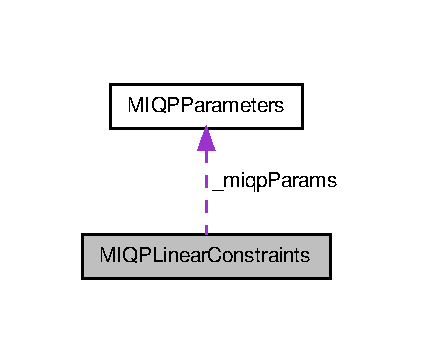
\includegraphics[width=203pt]{classMIQPLinearConstraints__coll__graph}
\end{center}
\end{figure}
\subsection*{\-Public \-Member \-Functions}
\begin{DoxyCompactItemize}
\item 
\hyperlink{classMIQPLinearConstraints_aaa55e8fc7fac6499f60c40e13b0d6605}{\-M\-I\-Q\-P\-Linear\-Constraints} (std\-::shared\-\_\-ptr$<$ \hyperlink{classStepController}{\-Step\-Controller} $>$ step\-Controller, \hyperlink{structMIQPParameters}{\-M\-I\-Q\-P\-Parameters} miqp\-Params, bool add\-Shape\-Ctrs=true, bool add\-Admissibility\-Ctrs=true, bool add\-Co\-P\-Constraints=false, bool add\-Walking\-Ctrs=false)
\item 
virtual \hyperlink{classMIQPLinearConstraints_a1539d3c8eb2af42daa9bb17dd0f44bd2}{$\sim$\-M\-I\-Q\-P\-Linear\-Constraints} ()
\item 
void \hyperlink{classMIQPLinearConstraints_a27ae3bdf1d4b4bd1e5279607e4b96f1a}{update\-R\-H\-S} (const \-Eigen\-::\-Vector\-Xd \&xi\-\_\-k)
\item 
void \hyperlink{classMIQPLinearConstraints_ab556e990dcc0b1fcd152f41a8c00e1f6}{get\-Constraints\-Matrix\-A} (\-Eigen\-::\-Matrix\-Xd \&\-A)
\item 
unsigned int \hyperlink{classMIQPLinearConstraints_a656681ab464709b025e4522df3458fa1}{get\-Total\-Number\-Of\-Constraints} ()
\item 
void \hyperlink{classMIQPLinearConstraints_abf2bd3e8f0dfa5b919efa1b90b56232a}{get\-R\-H\-S} (\-Eigen\-::\-Vector\-Xd \&rhs)
\end{DoxyCompactItemize}
\subsection*{\-Protected \-Member \-Functions}
\begin{DoxyCompactItemize}
\item 
void \hyperlink{classMIQPLinearConstraints_a2f41d99a16293718b94d17ce9ee5b59d}{build\-Shape\-And\-Admissibility\-In\-Preview\-Window} ()
\item 
void \hyperlink{classMIQPLinearConstraints_ae9b8c02ee58863d05d2aab41e780413e}{build\-A\-Shape\-Admiss} ()
\item 
void \hyperlink{classMIQPLinearConstraints_aa3752e85f1167129814b1a41d6b0198e}{build\-B\-Shape\-Admiss} ()
\item 
void \hyperlink{classMIQPLinearConstraints_a5231950d561e42e0d6590a398bec771c}{build\-Fc\-Bar\-Shape\-Admiss} ()
\item 
void \hyperlink{classMIQPLinearConstraints_ad36868550b3d1f977a67e76a44160192}{set\-Matrix\-Acr} ()
\item 
void \hyperlink{classMIQPLinearConstraints_a2985d200d8e6baba2df17abfeaca8882}{set\-Matrix\-Acl} ()
\item 
void \hyperlink{classMIQPLinearConstraints_a127e7ddd641f11d1b6137c59d80ef8b5}{build\-Matrix\-Q} ()
\item 
void \hyperlink{classMIQPLinearConstraints_addee397c47be26fd9eebbe8374c3cc30}{build\-Matrix\-T} ()
\item 
void \hyperlink{classMIQPLinearConstraints_ae6ecdf8d77474a8b099f2526d6cc0d75}{build\-Bh} ()
\item 
void \hyperlink{classMIQPLinearConstraints_a70bcc70db0ab171390d20af674e80c27}{build\-Ah} ()
\end{DoxyCompactItemize}
\subsection*{\-Private \-Attributes}
\begin{DoxyCompactItemize}
\item 
std\-::shared\-\_\-ptr$<$ \hyperlink{classShapeConstraints}{\-Shape\-Constraints} $>$ \hyperlink{classMIQPLinearConstraints_a5c8788e52f7b0664606662cfa758ae88}{\-\_\-shape\-Cnstr}
\item 
std\-::shared\-\_\-ptr\*
$<$ \hyperlink{classAdmissibilityConstraints}{\-Admissibility\-Constraints} $>$ \hyperlink{classMIQPLinearConstraints_a1ac00fe6aca254b4dd8568e199bd20a4}{\-\_\-admissibility\-Cnstr}
\item 
std\-::shared\-\_\-ptr$<$ \hyperlink{classStepController}{\-Step\-Controller} $>$ \hyperlink{classMIQPLinearConstraints_ac1ea7dbfb54c84c9c3e172d36aa42671}{\-\_\-step\-Controller}
\item 
\-Eigen\-::\-Matrix\-Xd \hyperlink{classMIQPLinearConstraints_a7ff7b3584cf9ff3e2124d80bd0684180}{\-\_\-\-A\-Shape\-Admiss}
\item 
\-Eigen\-::\-Matrix\-Xd \hyperlink{classMIQPLinearConstraints_ab3ea8be40c22fa7d8035c7b5c5c1010c}{\-\_\-\-B\-Shape\-Admiss}
\item 
\-Eigen\-::\-Vector\-Xd \hyperlink{classMIQPLinearConstraints_a4e1cac634590c04e81d9b9341088efeb}{\-\_\-fcbar\-Shape\-Admiss}
\item 
\-Eigen\-::\-Matrix\-Xd \hyperlink{classMIQPLinearConstraints_a5dfdc7553c4cbbe75ac54b34c4f29732}{\-\_\-\-A}
\item 
\-Eigen\-::\-Vector\-Xd \hyperlink{classMIQPLinearConstraints_ac8df74075c393100f5bddcb371503530}{\-\_\-rhs}
\item 
\-Eigen\-::\-Matrix\-Xd \hyperlink{classMIQPLinearConstraints_a26250a3f878cdacc0fa0c5ccf04d0bed}{\-\_\-\-Acr}
\item 
\-Eigen\-::\-Matrix\-Xd \hyperlink{classMIQPLinearConstraints_a100ca667cae697cda19ae4aef3543120}{\-\_\-\-Acl}
\item 
\-Eigen\-::\-Matrix\-Xd \hyperlink{classMIQPLinearConstraints_afecaf6e02135bfba45045fab6cce3511}{\-\_\-\-Q}
\item 
\-Eigen\-::\-Matrix\-Xd \hyperlink{classMIQPLinearConstraints_a5e6d37521f3da248b19ff424526d700a}{\-\_\-\-T}
\item 
\-Eigen\-::\-Matrix\-Xd \hyperlink{classMIQPLinearConstraints_a0c0fbbb1b86c5d51a133ee661977c1f5}{\-\_\-\-Bh}
\item 
\-Eigen\-::\-Matrix\-Xd \hyperlink{classMIQPLinearConstraints_aacba15c9dfc1c8f88e253a4f75e422fd}{\-\_\-\-Ah}
\item 
bool \hyperlink{classMIQPLinearConstraints_ae8df8b83e80484853b624f6693ed2725}{\-\_\-add\-Shape\-Ctrs}
\item 
bool \hyperlink{classMIQPLinearConstraints_a155ab4ad5ab14b793611c12473ce9297}{\-\_\-add\-Admissibility\-Ctrs}
\item 
bool \hyperlink{classMIQPLinearConstraints_a8e20d42828c638f41d074153cc0957d8}{\-\_\-add\-Co\-P\-Constraints}
\item 
bool \hyperlink{classMIQPLinearConstraints_ad1363c7fde3dd4f20adc92a7e1865579}{\-\_\-add\-Walking\-Ctrs}
\item 
unsigned int \hyperlink{classMIQPLinearConstraints_a403b0a1f684bda20236a759bd72950f2}{\-\_\-dt}
\item 
unsigned int \hyperlink{classMIQPLinearConstraints_a1edaf84d613dde3f86fd9e78aa14a077}{\-\_\-\-N}
\item 
unsigned int \hyperlink{classMIQPLinearConstraints_a2726424eb890fe556ce503096b418d0f}{\-\_\-n\-Constraints}
\item 
std\-::shared\-\_\-ptr$<$ \hyperlink{classBaseOfSupport}{\-Base\-Of\-Support} $>$ \hyperlink{classMIQPLinearConstraints_a9b26abbc012b0f39c6bef163d9c3faed}{\-\_\-base\-Of\-Support}
\item 
\hyperlink{structMIQPParameters}{\-M\-I\-Q\-P\-Parameters} \hyperlink{classMIQPLinearConstraints_a22f1b42e65d283a0d748333cc7119a7e}{\-\_\-miqp\-Params}
\end{DoxyCompactItemize}


\subsection{\-Constructor \& \-Destructor \-Documentation}
\hypertarget{classMIQPLinearConstraints_aaa55e8fc7fac6499f60c40e13b0d6605}{\index{\-M\-I\-Q\-P\-Linear\-Constraints@{\-M\-I\-Q\-P\-Linear\-Constraints}!\-M\-I\-Q\-P\-Linear\-Constraints@{\-M\-I\-Q\-P\-Linear\-Constraints}}
\index{\-M\-I\-Q\-P\-Linear\-Constraints@{\-M\-I\-Q\-P\-Linear\-Constraints}!MIQPLinearConstraints@{\-M\-I\-Q\-P\-Linear\-Constraints}}
\subsubsection[{\-M\-I\-Q\-P\-Linear\-Constraints}]{\setlength{\rightskip}{0pt plus 5cm}{\bf \-M\-I\-Q\-P\-Linear\-Constraints\-::\-M\-I\-Q\-P\-Linear\-Constraints} (
\begin{DoxyParamCaption}
\item[{std\-::shared\-\_\-ptr$<$ {\bf \-Step\-Controller} $>$}]{step\-Controller, }
\item[{{\bf \-M\-I\-Q\-P\-Parameters}}]{miqp\-Params, }
\item[{bool}]{add\-Shape\-Ctrs = {\ttfamily true}, }
\item[{bool}]{add\-Admissibility\-Ctrs = {\ttfamily true}, }
\item[{bool}]{add\-Co\-P\-Constraints = {\ttfamily false}, }
\item[{bool}]{add\-Walking\-Ctrs = {\ttfamily false}}
\end{DoxyParamCaption}
)}}\label{classMIQPLinearConstraints_aaa55e8fc7fac6499f60c40e13b0d6605}
\begin{DoxyRefDesc}{\-Todo}
\item[\hyperlink{todo__todo000004}{\-Todo}]\-Once \-I add walking constraints this will change to include the rows added by walking constraints \end{DoxyRefDesc}

\begin{DoxyParams}[1]{\-Parameters}
\mbox{\tt in}  & {\em step\-Controller} & \-Pointer to \hyperlink{classStepController}{\-Step\-Controller} object which is instantiated by the hosting client. \\
\hline
\mbox{\tt in}  & {\em miqp\-Params} & \-Container of the \hyperlink{namespaceMIQP}{\-M\-I\-Q\-P} parameters. \\
\hline
\mbox{\tt in}  & {\em add\-Shape\-Ctrs} & \-Boolean indicating whether shape constraints are added to the problem. \\
\hline
\mbox{\tt in}  & {\em add\-Admissibility\-Ctrs} & \-Boolean indicating whether admissibility constraints are added to the problem. \\
\hline
\mbox{\tt in}  & {\em add\-Co\-P\-Constraints} & \-Boolean indicating whether \-Co\-P constraints are added to the problem. \\
\hline
\mbox{\tt in}  & {\em add\-Walking\-Ctrs} & \-Boolean indicating whether walking constraints are added to the problem.\\
\hline
\end{DoxyParams}
\begin{DoxyRefDesc}{\-Todo}
\item[\hyperlink{todo__todo000005}{\-Todo}]\-Handle the booleans in a different form. \-This is sort of ugly. \end{DoxyRefDesc}
\hypertarget{classMIQPLinearConstraints_a1539d3c8eb2af42daa9bb17dd0f44bd2}{\index{\-M\-I\-Q\-P\-Linear\-Constraints@{\-M\-I\-Q\-P\-Linear\-Constraints}!$\sim$\-M\-I\-Q\-P\-Linear\-Constraints@{$\sim$\-M\-I\-Q\-P\-Linear\-Constraints}}
\index{$\sim$\-M\-I\-Q\-P\-Linear\-Constraints@{$\sim$\-M\-I\-Q\-P\-Linear\-Constraints}!MIQPLinearConstraints@{\-M\-I\-Q\-P\-Linear\-Constraints}}
\subsubsection[{$\sim$\-M\-I\-Q\-P\-Linear\-Constraints}]{\setlength{\rightskip}{0pt plus 5cm}{\bf \-M\-I\-Q\-P\-Linear\-Constraints\-::$\sim$\-M\-I\-Q\-P\-Linear\-Constraints} (
\begin{DoxyParamCaption}
{}
\end{DoxyParamCaption}
)\hspace{0.3cm}{\ttfamily  \mbox{[}virtual\mbox{]}}}}\label{classMIQPLinearConstraints_a1539d3c8eb2af42daa9bb17dd0f44bd2}
\-Default destructor 

\subsection{\-Member \-Function \-Documentation}
\hypertarget{classMIQPLinearConstraints_a70bcc70db0ab171390d20af674e80c27}{\index{\-M\-I\-Q\-P\-Linear\-Constraints@{\-M\-I\-Q\-P\-Linear\-Constraints}!build\-Ah@{build\-Ah}}
\index{build\-Ah@{build\-Ah}!MIQPLinearConstraints@{\-M\-I\-Q\-P\-Linear\-Constraints}}
\subsubsection[{build\-Ah}]{\setlength{\rightskip}{0pt plus 5cm}void {\bf \-M\-I\-Q\-P\-Linear\-Constraints\-::build\-Ah} (
\begin{DoxyParamCaption}
{}
\end{DoxyParamCaption}
)\hspace{0.3cm}{\ttfamily  \mbox{[}protected\mbox{]}}}}\label{classMIQPLinearConstraints_a70bcc70db0ab171390d20af674e80c27}
\-Builds $A_h$.

\begin{DoxySeeAlso}{\-See also}
\hyperlink{classMIQPLinearConstraints_aacba15c9dfc1c8f88e253a4f75e422fd}{\-\_\-\-Ah} 
\end{DoxySeeAlso}
\hypertarget{classMIQPLinearConstraints_ae9b8c02ee58863d05d2aab41e780413e}{\index{\-M\-I\-Q\-P\-Linear\-Constraints@{\-M\-I\-Q\-P\-Linear\-Constraints}!build\-A\-Shape\-Admiss@{build\-A\-Shape\-Admiss}}
\index{build\-A\-Shape\-Admiss@{build\-A\-Shape\-Admiss}!MIQPLinearConstraints@{\-M\-I\-Q\-P\-Linear\-Constraints}}
\subsubsection[{build\-A\-Shape\-Admiss}]{\setlength{\rightskip}{0pt plus 5cm}void {\bf \-M\-I\-Q\-P\-Linear\-Constraints\-::build\-A\-Shape\-Admiss} (
\begin{DoxyParamCaption}
{}
\end{DoxyParamCaption}
)\hspace{0.3cm}{\ttfamily  \mbox{[}protected\mbox{]}}}}\label{classMIQPLinearConstraints_ae9b8c02ee58863d05d2aab41e780413e}
\-Actually builds the matrix \-A referred to in \hyperlink{classMIQPLinearConstraints_a2f41d99a16293718b94d17ce9ee5b59d}{build\-Shape\-And\-Admissibility\-In\-Preview\-Window()}

\begin{DoxySeeAlso}{\-See also}
\hyperlink{classMIQPLinearConstraints_a2f41d99a16293718b94d17ce9ee5b59d}{build\-Shape\-And\-Admissibility\-In\-Preview\-Window} 
\end{DoxySeeAlso}
\hypertarget{classMIQPLinearConstraints_ae6ecdf8d77474a8b099f2526d6cc0d75}{\index{\-M\-I\-Q\-P\-Linear\-Constraints@{\-M\-I\-Q\-P\-Linear\-Constraints}!build\-Bh@{build\-Bh}}
\index{build\-Bh@{build\-Bh}!MIQPLinearConstraints@{\-M\-I\-Q\-P\-Linear\-Constraints}}
\subsubsection[{build\-Bh}]{\setlength{\rightskip}{0pt plus 5cm}void {\bf \-M\-I\-Q\-P\-Linear\-Constraints\-::build\-Bh} (
\begin{DoxyParamCaption}
{}
\end{DoxyParamCaption}
)\hspace{0.3cm}{\ttfamily  \mbox{[}protected\mbox{]}}}}\label{classMIQPLinearConstraints_ae6ecdf8d77474a8b099f2526d6cc0d75}
\-Builds $B_h$ (\hyperlink{classMIQPLinearConstraints_a0c0fbbb1b86c5d51a133ee661977c1f5}{\-\_\-\-Bh}) called by the constructor of this class.

\begin{DoxySeeAlso}{\-See also}
\hyperlink{classMIQPLinearConstraints_a0c0fbbb1b86c5d51a133ee661977c1f5}{\-\_\-\-Bh} 
\end{DoxySeeAlso}
\hypertarget{classMIQPLinearConstraints_aa3752e85f1167129814b1a41d6b0198e}{\index{\-M\-I\-Q\-P\-Linear\-Constraints@{\-M\-I\-Q\-P\-Linear\-Constraints}!build\-B\-Shape\-Admiss@{build\-B\-Shape\-Admiss}}
\index{build\-B\-Shape\-Admiss@{build\-B\-Shape\-Admiss}!MIQPLinearConstraints@{\-M\-I\-Q\-P\-Linear\-Constraints}}
\subsubsection[{build\-B\-Shape\-Admiss}]{\setlength{\rightskip}{0pt plus 5cm}void {\bf \-M\-I\-Q\-P\-Linear\-Constraints\-::build\-B\-Shape\-Admiss} (
\begin{DoxyParamCaption}
{}
\end{DoxyParamCaption}
)\hspace{0.3cm}{\ttfamily  \mbox{[}protected\mbox{]}}}}\label{classMIQPLinearConstraints_aa3752e85f1167129814b1a41d6b0198e}
\-Actually builds the matrix \-B referred to in \hyperlink{classMIQPLinearConstraints_a2f41d99a16293718b94d17ce9ee5b59d}{build\-Shape\-And\-Admissibility\-In\-Preview\-Window()}

\begin{DoxySeeAlso}{\-See also}
\hyperlink{classMIQPLinearConstraints_a2f41d99a16293718b94d17ce9ee5b59d}{build\-Shape\-And\-Admissibility\-In\-Preview\-Window} 
\end{DoxySeeAlso}
\hypertarget{classMIQPLinearConstraints_a5231950d561e42e0d6590a398bec771c}{\index{\-M\-I\-Q\-P\-Linear\-Constraints@{\-M\-I\-Q\-P\-Linear\-Constraints}!build\-Fc\-Bar\-Shape\-Admiss@{build\-Fc\-Bar\-Shape\-Admiss}}
\index{build\-Fc\-Bar\-Shape\-Admiss@{build\-Fc\-Bar\-Shape\-Admiss}!MIQPLinearConstraints@{\-M\-I\-Q\-P\-Linear\-Constraints}}
\subsubsection[{build\-Fc\-Bar\-Shape\-Admiss}]{\setlength{\rightskip}{0pt plus 5cm}void {\bf \-M\-I\-Q\-P\-Linear\-Constraints\-::build\-Fc\-Bar\-Shape\-Admiss} (
\begin{DoxyParamCaption}
{}
\end{DoxyParamCaption}
)\hspace{0.3cm}{\ttfamily  \mbox{[}protected\mbox{]}}}}\label{classMIQPLinearConstraints_a5231950d561e42e0d6590a398bec771c}
\-Actually builds the vector $\bar{\mathbf{f}}_c$ referred to in \hyperlink{classMIQPLinearConstraints_a2f41d99a16293718b94d17ce9ee5b59d}{build\-Shape\-And\-Admissibility\-In\-Preview\-Window()} \hypertarget{classMIQPLinearConstraints_a127e7ddd641f11d1b6137c59d80ef8b5}{\index{\-M\-I\-Q\-P\-Linear\-Constraints@{\-M\-I\-Q\-P\-Linear\-Constraints}!build\-Matrix\-Q@{build\-Matrix\-Q}}
\index{build\-Matrix\-Q@{build\-Matrix\-Q}!MIQPLinearConstraints@{\-M\-I\-Q\-P\-Linear\-Constraints}}
\subsubsection[{build\-Matrix\-Q}]{\setlength{\rightskip}{0pt plus 5cm}void {\bf \-M\-I\-Q\-P\-Linear\-Constraints\-::build\-Matrix\-Q} (
\begin{DoxyParamCaption}
{}
\end{DoxyParamCaption}
)\hspace{0.3cm}{\ttfamily  \mbox{[}protected\mbox{]}}}}\label{classMIQPLinearConstraints_a127e7ddd641f11d1b6137c59d80ef8b5}
\-Builds matrix \-Q (\hyperlink{classMIQPLinearConstraints_afecaf6e02135bfba45045fab6cce3511}{\-\_\-\-Q}) from the preview model\-:

\[ \forall j \in \mathbb{N}^*, \xi_{k+j+1|k} = \mathbf{Q} \xi_{k+j|k} + \mathbf{T}\mathcal{X}_{k+j+1|k} \] \hypertarget{classMIQPLinearConstraints_addee397c47be26fd9eebbe8374c3cc30}{\index{\-M\-I\-Q\-P\-Linear\-Constraints@{\-M\-I\-Q\-P\-Linear\-Constraints}!build\-Matrix\-T@{build\-Matrix\-T}}
\index{build\-Matrix\-T@{build\-Matrix\-T}!MIQPLinearConstraints@{\-M\-I\-Q\-P\-Linear\-Constraints}}
\subsubsection[{build\-Matrix\-T}]{\setlength{\rightskip}{0pt plus 5cm}void {\bf \-M\-I\-Q\-P\-Linear\-Constraints\-::build\-Matrix\-T} (
\begin{DoxyParamCaption}
{}
\end{DoxyParamCaption}
)\hspace{0.3cm}{\ttfamily  \mbox{[}protected\mbox{]}}}}\label{classMIQPLinearConstraints_addee397c47be26fd9eebbe8374c3cc30}
\-Builds matrix \-T (\hyperlink{classMIQPLinearConstraints_a5e6d37521f3da248b19ff424526d700a}{\-\_\-\-T}) from the preview model\-:

\[ \forall j \in \mathbb{N}^*, \xi_{k+j+1|k} = \mathbf{Q} \xi_{k+j|k} + \mathbf{T}\mathcal{X}_{k+j+1|k} \] \hypertarget{classMIQPLinearConstraints_a2f41d99a16293718b94d17ce9ee5b59d}{\index{\-M\-I\-Q\-P\-Linear\-Constraints@{\-M\-I\-Q\-P\-Linear\-Constraints}!build\-Shape\-And\-Admissibility\-In\-Preview\-Window@{build\-Shape\-And\-Admissibility\-In\-Preview\-Window}}
\index{build\-Shape\-And\-Admissibility\-In\-Preview\-Window@{build\-Shape\-And\-Admissibility\-In\-Preview\-Window}!MIQPLinearConstraints@{\-M\-I\-Q\-P\-Linear\-Constraints}}
\subsubsection[{build\-Shape\-And\-Admissibility\-In\-Preview\-Window}]{\setlength{\rightskip}{0pt plus 5cm}void {\bf \-M\-I\-Q\-P\-Linear\-Constraints\-::build\-Shape\-And\-Admissibility\-In\-Preview\-Window} (
\begin{DoxyParamCaption}
{}
\end{DoxyParamCaption}
)\hspace{0.3cm}{\ttfamily  \mbox{[}protected\mbox{]}}}}\label{classMIQPLinearConstraints_a2f41d99a16293718b94d17ce9ee5b59d}
\-Basically builds matrix $\mathbf{A}$ (\hyperlink{classMIQPLinearConstraints_a7ff7b3584cf9ff3e2124d80bd0684180}{\-\_\-\-A\-Shape\-Admiss}) in the partial expression for the \hyperlink{namespaceMIQP}{\-M\-I\-Q\-P} linear constraints, containing only shape and admissibility constraints, such that\-: \[ \mathbf{A} \mathcal{X}_{k,N} \leq \bar{\mathbf{f}}_c - \mathbf{B} \xi_k \]

\[ \begin{array}{cccccc} A_{\text{cr}} Q^0 T & 0 & 0 & 0 & \hdots & 0\\ (A_{\text{cl}}Q^0 + A_{\text{cr}}Q^1)T & A_{\text{cr}}Q^0 T & 0 & 0 & \hdots & 0 \\ (A_{\text{cl}}Q^1 + A_{\text{cr}}Q^2)T & (A_{\text{cl}}Q^0 + A_{\text{cr}}Q^1)T & A_{\text{cr}} Q^0 T & 0 & \hdots & 0 \\ \vdots & \vdots & & & & \vdots \\ (A_{\text{cl}}Q^{N-2} + A_{\text{cr}}Q^{N-1})T & (A_{\text{cl}}Q^{N-3} + A_{\text{cr}}Q^{N-2})T & \hdots & \hdots & \hdots & A_{\text{cr}}Q^0T \\ \end{array} \]

\begin{DoxySeeAlso}{\-See also}
\hyperlink{classMIQPLinearConstraints_ae9b8c02ee58863d05d2aab41e780413e}{build\-A\-Shape\-Admiss()} 
\end{DoxySeeAlso}
\begin{DoxyRefDesc}{\-Todo}
\item[\hyperlink{todo__todo000006}{\-Todo}]\-When walking constraints are added, matrix \-\_\-\-A will be a stack of the two \end{DoxyRefDesc}
\hypertarget{classMIQPLinearConstraints_ab556e990dcc0b1fcd152f41a8c00e1f6}{\index{\-M\-I\-Q\-P\-Linear\-Constraints@{\-M\-I\-Q\-P\-Linear\-Constraints}!get\-Constraints\-Matrix\-A@{get\-Constraints\-Matrix\-A}}
\index{get\-Constraints\-Matrix\-A@{get\-Constraints\-Matrix\-A}!MIQPLinearConstraints@{\-M\-I\-Q\-P\-Linear\-Constraints}}
\subsubsection[{get\-Constraints\-Matrix\-A}]{\setlength{\rightskip}{0pt plus 5cm}void {\bf \-M\-I\-Q\-P\-Linear\-Constraints\-::get\-Constraints\-Matrix\-A} (
\begin{DoxyParamCaption}
\item[{\-Eigen\-::\-Matrix\-Xd \&}]{\-A}
\end{DoxyParamCaption}
)}}\label{classMIQPLinearConstraints_ab556e990dcc0b1fcd152f41a8c00e1f6}
\-Retrieves the constraints matrix $\mathbf{A}$. \-Before passing a matrix to copy \hyperlink{classMIQPLinearConstraints_a5dfdc7553c4cbbe75ac54b34c4f29732}{\-\_\-\-A} allocate the space for \-A by calling \hyperlink{classMIQPLinearConstraints_a656681ab464709b025e4522df3458fa1}{get\-Total\-Number\-Of\-Constraints()} to know the number of rows, while \-I\-N\-P\-U\-T\-\_\-\-V\-E\-C\-T\-O\-R\-\_\-\-S\-I\-Z\-E $\ast$ \-S\-I\-Z\-E\-\_\-\-P\-R\-E\-V\-I\-E\-W\-\_\-\-W\-I\-N\-D\-O\-W will be the number of columns.


\begin{DoxyParams}{\-Parameters}
{\em \-A} & \-Reference to matrix where the global constraints matrix \-\_\-\-A will be copied. \\
\hline
\end{DoxyParams}
\hypertarget{classMIQPLinearConstraints_abf2bd3e8f0dfa5b919efa1b90b56232a}{\index{\-M\-I\-Q\-P\-Linear\-Constraints@{\-M\-I\-Q\-P\-Linear\-Constraints}!get\-R\-H\-S@{get\-R\-H\-S}}
\index{get\-R\-H\-S@{get\-R\-H\-S}!MIQPLinearConstraints@{\-M\-I\-Q\-P\-Linear\-Constraints}}
\subsubsection[{get\-R\-H\-S}]{\setlength{\rightskip}{0pt plus 5cm}void {\bf \-M\-I\-Q\-P\-Linear\-Constraints\-::get\-R\-H\-S} (
\begin{DoxyParamCaption}
\item[{\-Eigen\-::\-Vector\-Xd \&}]{rhs}
\end{DoxyParamCaption}
)}}\label{classMIQPLinearConstraints_abf2bd3e8f0dfa5b919efa1b90b56232a}
\-Returns in \#rhs the right-\/hand size of the inequality constraints of the problem.


\begin{DoxyParams}[1]{\-Parameters}
\mbox{\tt out}  & {\em rhs} & \-State-\/dependent right hand side. \\
\hline
\end{DoxyParams}
\begin{DoxySeeAlso}{\-See also}
\hyperlink{classMIQPLinearConstraints_a27ae3bdf1d4b4bd1e5279607e4b96f1a}{update\-R\-H\-S()} 
\end{DoxySeeAlso}
\hypertarget{classMIQPLinearConstraints_a656681ab464709b025e4522df3458fa1}{\index{\-M\-I\-Q\-P\-Linear\-Constraints@{\-M\-I\-Q\-P\-Linear\-Constraints}!get\-Total\-Number\-Of\-Constraints@{get\-Total\-Number\-Of\-Constraints}}
\index{get\-Total\-Number\-Of\-Constraints@{get\-Total\-Number\-Of\-Constraints}!MIQPLinearConstraints@{\-M\-I\-Q\-P\-Linear\-Constraints}}
\subsubsection[{get\-Total\-Number\-Of\-Constraints}]{\setlength{\rightskip}{0pt plus 5cm}unsigned int {\bf \-M\-I\-Q\-P\-Linear\-Constraints\-::get\-Total\-Number\-Of\-Constraints} (
\begin{DoxyParamCaption}
{}
\end{DoxyParamCaption}
)}}\label{classMIQPLinearConstraints_a656681ab464709b025e4522df3458fa1}
\-Returns the total number of constraints.

\begin{DoxyReturn}{\-Returns}
\-\_\-n\-Constraints 
\end{DoxyReturn}
\hypertarget{classMIQPLinearConstraints_a2985d200d8e6baba2df17abfeaca8882}{\index{\-M\-I\-Q\-P\-Linear\-Constraints@{\-M\-I\-Q\-P\-Linear\-Constraints}!set\-Matrix\-Acl@{set\-Matrix\-Acl}}
\index{set\-Matrix\-Acl@{set\-Matrix\-Acl}!MIQPLinearConstraints@{\-M\-I\-Q\-P\-Linear\-Constraints}}
\subsubsection[{set\-Matrix\-Acl}]{\setlength{\rightskip}{0pt plus 5cm}void {\bf \-M\-I\-Q\-P\-Linear\-Constraints\-::set\-Matrix\-Acl} (
\begin{DoxyParamCaption}
{}
\end{DoxyParamCaption}
)\hspace{0.3cm}{\ttfamily  \mbox{[}protected\mbox{]}}}}\label{classMIQPLinearConstraints_a2985d200d8e6baba2df17abfeaca8882}
\-Stacks matrices $C_{i}$ (\-Ci) from the shape and admissiblity constraints to set variable \hyperlink{classMIQPLinearConstraints_a100ca667cae697cda19ae4aef3543120}{\-\_\-\-Acl} \hypertarget{classMIQPLinearConstraints_ad36868550b3d1f977a67e76a44160192}{\index{\-M\-I\-Q\-P\-Linear\-Constraints@{\-M\-I\-Q\-P\-Linear\-Constraints}!set\-Matrix\-Acr@{set\-Matrix\-Acr}}
\index{set\-Matrix\-Acr@{set\-Matrix\-Acr}!MIQPLinearConstraints@{\-M\-I\-Q\-P\-Linear\-Constraints}}
\subsubsection[{set\-Matrix\-Acr}]{\setlength{\rightskip}{0pt plus 5cm}void {\bf \-M\-I\-Q\-P\-Linear\-Constraints\-::set\-Matrix\-Acr} (
\begin{DoxyParamCaption}
{}
\end{DoxyParamCaption}
)\hspace{0.3cm}{\ttfamily  \mbox{[}protected\mbox{]}}}}\label{classMIQPLinearConstraints_ad36868550b3d1f977a67e76a44160192}
\-Stacks matrices $C_{i+1}$ (\-Cii) from the shape and admissibility constraints to set variable \hyperlink{classMIQPLinearConstraints_a26250a3f878cdacc0fa0c5ccf04d0bed}{\-\_\-\-Acr} \hypertarget{classMIQPLinearConstraints_a27ae3bdf1d4b4bd1e5279607e4b96f1a}{\index{\-M\-I\-Q\-P\-Linear\-Constraints@{\-M\-I\-Q\-P\-Linear\-Constraints}!update\-R\-H\-S@{update\-R\-H\-S}}
\index{update\-R\-H\-S@{update\-R\-H\-S}!MIQPLinearConstraints@{\-M\-I\-Q\-P\-Linear\-Constraints}}
\subsubsection[{update\-R\-H\-S}]{\setlength{\rightskip}{0pt plus 5cm}void {\bf \-M\-I\-Q\-P\-Linear\-Constraints\-::update\-R\-H\-S} (
\begin{DoxyParamCaption}
\item[{const \-Eigen\-::\-Vector\-Xd \&}]{xi\-\_\-k}
\end{DoxyParamCaption}
)}}\label{classMIQPLinearConstraints_a27ae3bdf1d4b4bd1e5279607e4b96f1a}
\-Updates the state-\/dependent \-R\-H\-S of the inequality constraints


\begin{DoxyParams}[1]{\-Parameters}
\mbox{\tt in}  & {\em xi\-\_\-k} & \-Current state. \\
\hline
\end{DoxyParams}
\-F\-I\-X\-M\-E\-: \-T\-E\-M\-P\-O\-R\-A\-R\-Y!! \-Maybe it's best to have a more generic update method 

\subsection{\-Member \-Data \-Documentation}
\hypertarget{classMIQPLinearConstraints_a5dfdc7553c4cbbe75ac54b34c4f29732}{\index{\-M\-I\-Q\-P\-Linear\-Constraints@{\-M\-I\-Q\-P\-Linear\-Constraints}!\-\_\-\-A@{\-\_\-\-A}}
\index{\-\_\-\-A@{\-\_\-\-A}!MIQPLinearConstraints@{\-M\-I\-Q\-P\-Linear\-Constraints}}
\subsubsection[{\-\_\-\-A}]{\setlength{\rightskip}{0pt plus 5cm}\-Eigen\-::\-Matrix\-Xd {\bf \-M\-I\-Q\-P\-Linear\-Constraints\-::\-\_\-\-A}\hspace{0.3cm}{\ttfamily  \mbox{[}private\mbox{]}}}}\label{classMIQPLinearConstraints_a5dfdc7553c4cbbe75ac54b34c4f29732}
\hypertarget{classMIQPLinearConstraints_a100ca667cae697cda19ae4aef3543120}{\index{\-M\-I\-Q\-P\-Linear\-Constraints@{\-M\-I\-Q\-P\-Linear\-Constraints}!\-\_\-\-Acl@{\-\_\-\-Acl}}
\index{\-\_\-\-Acl@{\-\_\-\-Acl}!MIQPLinearConstraints@{\-M\-I\-Q\-P\-Linear\-Constraints}}
\subsubsection[{\-\_\-\-Acl}]{\setlength{\rightskip}{0pt plus 5cm}\-Eigen\-::\-Matrix\-Xd {\bf \-M\-I\-Q\-P\-Linear\-Constraints\-::\-\_\-\-Acl}\hspace{0.3cm}{\ttfamily  \mbox{[}private\mbox{]}}}}\label{classMIQPLinearConstraints_a100ca667cae697cda19ae4aef3543120}
\hypertarget{classMIQPLinearConstraints_a26250a3f878cdacc0fa0c5ccf04d0bed}{\index{\-M\-I\-Q\-P\-Linear\-Constraints@{\-M\-I\-Q\-P\-Linear\-Constraints}!\-\_\-\-Acr@{\-\_\-\-Acr}}
\index{\-\_\-\-Acr@{\-\_\-\-Acr}!MIQPLinearConstraints@{\-M\-I\-Q\-P\-Linear\-Constraints}}
\subsubsection[{\-\_\-\-Acr}]{\setlength{\rightskip}{0pt plus 5cm}\-Eigen\-::\-Matrix\-Xd {\bf \-M\-I\-Q\-P\-Linear\-Constraints\-::\-\_\-\-Acr}\hspace{0.3cm}{\ttfamily  \mbox{[}private\mbox{]}}}}\label{classMIQPLinearConstraints_a26250a3f878cdacc0fa0c5ccf04d0bed}
\hypertarget{classMIQPLinearConstraints_a155ab4ad5ab14b793611c12473ce9297}{\index{\-M\-I\-Q\-P\-Linear\-Constraints@{\-M\-I\-Q\-P\-Linear\-Constraints}!\-\_\-add\-Admissibility\-Ctrs@{\-\_\-add\-Admissibility\-Ctrs}}
\index{\-\_\-add\-Admissibility\-Ctrs@{\-\_\-add\-Admissibility\-Ctrs}!MIQPLinearConstraints@{\-M\-I\-Q\-P\-Linear\-Constraints}}
\subsubsection[{\-\_\-add\-Admissibility\-Ctrs}]{\setlength{\rightskip}{0pt plus 5cm}bool {\bf \-M\-I\-Q\-P\-Linear\-Constraints\-::\-\_\-add\-Admissibility\-Ctrs}\hspace{0.3cm}{\ttfamily  \mbox{[}private\mbox{]}}}}\label{classMIQPLinearConstraints_a155ab4ad5ab14b793611c12473ce9297}
\-Boolean to add admissibility constraints. \hypertarget{classMIQPLinearConstraints_a8e20d42828c638f41d074153cc0957d8}{\index{\-M\-I\-Q\-P\-Linear\-Constraints@{\-M\-I\-Q\-P\-Linear\-Constraints}!\-\_\-add\-Co\-P\-Constraints@{\-\_\-add\-Co\-P\-Constraints}}
\index{\-\_\-add\-Co\-P\-Constraints@{\-\_\-add\-Co\-P\-Constraints}!MIQPLinearConstraints@{\-M\-I\-Q\-P\-Linear\-Constraints}}
\subsubsection[{\-\_\-add\-Co\-P\-Constraints}]{\setlength{\rightskip}{0pt plus 5cm}bool {\bf \-M\-I\-Q\-P\-Linear\-Constraints\-::\-\_\-add\-Co\-P\-Constraints}\hspace{0.3cm}{\ttfamily  \mbox{[}private\mbox{]}}}}\label{classMIQPLinearConstraints_a8e20d42828c638f41d074153cc0957d8}
\-Boolean to add \-Co\-P constraints within the convex hull defined by the feet location \hypertarget{classMIQPLinearConstraints_ae8df8b83e80484853b624f6693ed2725}{\index{\-M\-I\-Q\-P\-Linear\-Constraints@{\-M\-I\-Q\-P\-Linear\-Constraints}!\-\_\-add\-Shape\-Ctrs@{\-\_\-add\-Shape\-Ctrs}}
\index{\-\_\-add\-Shape\-Ctrs@{\-\_\-add\-Shape\-Ctrs}!MIQPLinearConstraints@{\-M\-I\-Q\-P\-Linear\-Constraints}}
\subsubsection[{\-\_\-add\-Shape\-Ctrs}]{\setlength{\rightskip}{0pt plus 5cm}bool {\bf \-M\-I\-Q\-P\-Linear\-Constraints\-::\-\_\-add\-Shape\-Ctrs}\hspace{0.3cm}{\ttfamily  \mbox{[}private\mbox{]}}}}\label{classMIQPLinearConstraints_ae8df8b83e80484853b624f6693ed2725}
\-Boolean too add shape constraints. \hypertarget{classMIQPLinearConstraints_ad1363c7fde3dd4f20adc92a7e1865579}{\index{\-M\-I\-Q\-P\-Linear\-Constraints@{\-M\-I\-Q\-P\-Linear\-Constraints}!\-\_\-add\-Walking\-Ctrs@{\-\_\-add\-Walking\-Ctrs}}
\index{\-\_\-add\-Walking\-Ctrs@{\-\_\-add\-Walking\-Ctrs}!MIQPLinearConstraints@{\-M\-I\-Q\-P\-Linear\-Constraints}}
\subsubsection[{\-\_\-add\-Walking\-Ctrs}]{\setlength{\rightskip}{0pt plus 5cm}bool {\bf \-M\-I\-Q\-P\-Linear\-Constraints\-::\-\_\-add\-Walking\-Ctrs}\hspace{0.3cm}{\ttfamily  \mbox{[}private\mbox{]}}}}\label{classMIQPLinearConstraints_ad1363c7fde3dd4f20adc92a7e1865579}
\-Boolean to add walking constraints. \hypertarget{classMIQPLinearConstraints_a1ac00fe6aca254b4dd8568e199bd20a4}{\index{\-M\-I\-Q\-P\-Linear\-Constraints@{\-M\-I\-Q\-P\-Linear\-Constraints}!\-\_\-admissibility\-Cnstr@{\-\_\-admissibility\-Cnstr}}
\index{\-\_\-admissibility\-Cnstr@{\-\_\-admissibility\-Cnstr}!MIQPLinearConstraints@{\-M\-I\-Q\-P\-Linear\-Constraints}}
\subsubsection[{\-\_\-admissibility\-Cnstr}]{\setlength{\rightskip}{0pt plus 5cm}std\-::shared\-\_\-ptr$<${\bf \-Admissibility\-Constraints}$>$ {\bf \-M\-I\-Q\-P\-Linear\-Constraints\-::\-\_\-admissibility\-Cnstr}\hspace{0.3cm}{\ttfamily  \mbox{[}private\mbox{]}}}}\label{classMIQPLinearConstraints_a1ac00fe6aca254b4dd8568e199bd20a4}
\hypertarget{classMIQPLinearConstraints_aacba15c9dfc1c8f88e253a4f75e422fd}{\index{\-M\-I\-Q\-P\-Linear\-Constraints@{\-M\-I\-Q\-P\-Linear\-Constraints}!\-\_\-\-Ah@{\-\_\-\-Ah}}
\index{\-\_\-\-Ah@{\-\_\-\-Ah}!MIQPLinearConstraints@{\-M\-I\-Q\-P\-Linear\-Constraints}}
\subsubsection[{\-\_\-\-Ah}]{\setlength{\rightskip}{0pt plus 5cm}\-Eigen\-::\-Matrix\-Xd {\bf \-M\-I\-Q\-P\-Linear\-Constraints\-::\-\_\-\-Ah}\hspace{0.3cm}{\ttfamily  \mbox{[}private\mbox{]}}}}\label{classMIQPLinearConstraints_aacba15c9dfc1c8f88e253a4f75e422fd}
\-State matrix $A_h$ from the \-Co\-M jerk integration scheme.

\[ \mathbf{h}_{k+1} = \mathbf{A}_h \mathbf{h}_k + \mathbf{B}_h \mathbf{u}_k \]

\-It is a constant matrix of size $6\times6$ equal to\-: \[ \mathbf{A_h} = \left[ \begin{array}{ccc} \mathbf{I}_2 & \delta t \mathbf{I}_2 & \frac{\delta t^2}{2} \mathbf{I}_2 \\ 0 & \mathbf{I}_2 & \delta t \mathbf{I}_2 \\ 0 & 0 & \mathbf{I}_2 \end{array} \right] \] \hypertarget{classMIQPLinearConstraints_a7ff7b3584cf9ff3e2124d80bd0684180}{\index{\-M\-I\-Q\-P\-Linear\-Constraints@{\-M\-I\-Q\-P\-Linear\-Constraints}!\-\_\-\-A\-Shape\-Admiss@{\-\_\-\-A\-Shape\-Admiss}}
\index{\-\_\-\-A\-Shape\-Admiss@{\-\_\-\-A\-Shape\-Admiss}!MIQPLinearConstraints@{\-M\-I\-Q\-P\-Linear\-Constraints}}
\subsubsection[{\-\_\-\-A\-Shape\-Admiss}]{\setlength{\rightskip}{0pt plus 5cm}\-Eigen\-::\-Matrix\-Xd {\bf \-M\-I\-Q\-P\-Linear\-Constraints\-::\-\_\-\-A\-Shape\-Admiss}\hspace{0.3cm}{\ttfamily  \mbox{[}private\mbox{]}}}}\label{classMIQPLinearConstraints_a7ff7b3584cf9ff3e2124d80bd0684180}
\hypertarget{classMIQPLinearConstraints_a9b26abbc012b0f39c6bef163d9c3faed}{\index{\-M\-I\-Q\-P\-Linear\-Constraints@{\-M\-I\-Q\-P\-Linear\-Constraints}!\-\_\-base\-Of\-Support@{\-\_\-base\-Of\-Support}}
\index{\-\_\-base\-Of\-Support@{\-\_\-base\-Of\-Support}!MIQPLinearConstraints@{\-M\-I\-Q\-P\-Linear\-Constraints}}
\subsubsection[{\-\_\-base\-Of\-Support}]{\setlength{\rightskip}{0pt plus 5cm}std\-::shared\-\_\-ptr$<${\bf \-Base\-Of\-Support}$>$ {\bf \-M\-I\-Q\-P\-Linear\-Constraints\-::\-\_\-base\-Of\-Support}\hspace{0.3cm}{\ttfamily  \mbox{[}private\mbox{]}}}}\label{classMIQPLinearConstraints_a9b26abbc012b0f39c6bef163d9c3faed}
\-Base of support object to retrieve the corresponding inequality constraints \hypertarget{classMIQPLinearConstraints_a0c0fbbb1b86c5d51a133ee661977c1f5}{\index{\-M\-I\-Q\-P\-Linear\-Constraints@{\-M\-I\-Q\-P\-Linear\-Constraints}!\-\_\-\-Bh@{\-\_\-\-Bh}}
\index{\-\_\-\-Bh@{\-\_\-\-Bh}!MIQPLinearConstraints@{\-M\-I\-Q\-P\-Linear\-Constraints}}
\subsubsection[{\-\_\-\-Bh}]{\setlength{\rightskip}{0pt plus 5cm}\-Eigen\-::\-Matrix\-Xd {\bf \-M\-I\-Q\-P\-Linear\-Constraints\-::\-\_\-\-Bh}\hspace{0.3cm}{\ttfamily  \mbox{[}private\mbox{]}}}}\label{classMIQPLinearConstraints_a0c0fbbb1b86c5d51a133ee661977c1f5}
\-Input matrix $\mathbf{B}_h$ from the linear state process of the \-Co\-Mstate $\hat{\mathbf{h}}$. \-It is constant of size $6\times2$ and equal to\-: \[ \mathbf{B_h} = \left[ \begin{array}{c} \frac{\delta^3}{6}\mathbf{I}_2 \\ \frac{\delta t^2}{2} \mathbf{I}_2 \\ \delta t \mathbf{I}_2 \end{array} \right] \] \hypertarget{classMIQPLinearConstraints_ab3ea8be40c22fa7d8035c7b5c5c1010c}{\index{\-M\-I\-Q\-P\-Linear\-Constraints@{\-M\-I\-Q\-P\-Linear\-Constraints}!\-\_\-\-B\-Shape\-Admiss@{\-\_\-\-B\-Shape\-Admiss}}
\index{\-\_\-\-B\-Shape\-Admiss@{\-\_\-\-B\-Shape\-Admiss}!MIQPLinearConstraints@{\-M\-I\-Q\-P\-Linear\-Constraints}}
\subsubsection[{\-\_\-\-B\-Shape\-Admiss}]{\setlength{\rightskip}{0pt plus 5cm}\-Eigen\-::\-Matrix\-Xd {\bf \-M\-I\-Q\-P\-Linear\-Constraints\-::\-\_\-\-B\-Shape\-Admiss}\hspace{0.3cm}{\ttfamily  \mbox{[}private\mbox{]}}}}\label{classMIQPLinearConstraints_ab3ea8be40c22fa7d8035c7b5c5c1010c}
\hypertarget{classMIQPLinearConstraints_a403b0a1f684bda20236a759bd72950f2}{\index{\-M\-I\-Q\-P\-Linear\-Constraints@{\-M\-I\-Q\-P\-Linear\-Constraints}!\-\_\-dt@{\-\_\-dt}}
\index{\-\_\-dt@{\-\_\-dt}!MIQPLinearConstraints@{\-M\-I\-Q\-P\-Linear\-Constraints}}
\subsubsection[{\-\_\-dt}]{\setlength{\rightskip}{0pt plus 5cm}unsigned int {\bf \-M\-I\-Q\-P\-Linear\-Constraints\-::\-\_\-dt}\hspace{0.3cm}{\ttfamily  \mbox{[}private\mbox{]}}}}\label{classMIQPLinearConstraints_a403b0a1f684bda20236a759bd72950f2}
\-Period in milliseconds \hypertarget{classMIQPLinearConstraints_a4e1cac634590c04e81d9b9341088efeb}{\index{\-M\-I\-Q\-P\-Linear\-Constraints@{\-M\-I\-Q\-P\-Linear\-Constraints}!\-\_\-fcbar\-Shape\-Admiss@{\-\_\-fcbar\-Shape\-Admiss}}
\index{\-\_\-fcbar\-Shape\-Admiss@{\-\_\-fcbar\-Shape\-Admiss}!MIQPLinearConstraints@{\-M\-I\-Q\-P\-Linear\-Constraints}}
\subsubsection[{\-\_\-fcbar\-Shape\-Admiss}]{\setlength{\rightskip}{0pt plus 5cm}\-Eigen\-::\-Vector\-Xd {\bf \-M\-I\-Q\-P\-Linear\-Constraints\-::\-\_\-fcbar\-Shape\-Admiss}\hspace{0.3cm}{\ttfamily  \mbox{[}private\mbox{]}}}}\label{classMIQPLinearConstraints_a4e1cac634590c04e81d9b9341088efeb}
\hypertarget{classMIQPLinearConstraints_a22f1b42e65d283a0d748333cc7119a7e}{\index{\-M\-I\-Q\-P\-Linear\-Constraints@{\-M\-I\-Q\-P\-Linear\-Constraints}!\-\_\-miqp\-Params@{\-\_\-miqp\-Params}}
\index{\-\_\-miqp\-Params@{\-\_\-miqp\-Params}!MIQPLinearConstraints@{\-M\-I\-Q\-P\-Linear\-Constraints}}
\subsubsection[{\-\_\-miqp\-Params}]{\setlength{\rightskip}{0pt plus 5cm}{\bf \-M\-I\-Q\-P\-Parameters} {\bf \-M\-I\-Q\-P\-Linear\-Constraints\-::\-\_\-miqp\-Params}\hspace{0.3cm}{\ttfamily  \mbox{[}private\mbox{]}}}}\label{classMIQPLinearConstraints_a22f1b42e65d283a0d748333cc7119a7e}
\hypertarget{classMIQPLinearConstraints_a1edaf84d613dde3f86fd9e78aa14a077}{\index{\-M\-I\-Q\-P\-Linear\-Constraints@{\-M\-I\-Q\-P\-Linear\-Constraints}!\-\_\-\-N@{\-\_\-\-N}}
\index{\-\_\-\-N@{\-\_\-\-N}!MIQPLinearConstraints@{\-M\-I\-Q\-P\-Linear\-Constraints}}
\subsubsection[{\-\_\-\-N}]{\setlength{\rightskip}{0pt plus 5cm}unsigned int {\bf \-M\-I\-Q\-P\-Linear\-Constraints\-::\-\_\-\-N}\hspace{0.3cm}{\ttfamily  \mbox{[}private\mbox{]}}}}\label{classMIQPLinearConstraints_a1edaf84d613dde3f86fd9e78aa14a077}
\-Length of preview window \hypertarget{classMIQPLinearConstraints_a2726424eb890fe556ce503096b418d0f}{\index{\-M\-I\-Q\-P\-Linear\-Constraints@{\-M\-I\-Q\-P\-Linear\-Constraints}!\-\_\-n\-Constraints@{\-\_\-n\-Constraints}}
\index{\-\_\-n\-Constraints@{\-\_\-n\-Constraints}!MIQPLinearConstraints@{\-M\-I\-Q\-P\-Linear\-Constraints}}
\subsubsection[{\-\_\-n\-Constraints}]{\setlength{\rightskip}{0pt plus 5cm}unsigned int {\bf \-M\-I\-Q\-P\-Linear\-Constraints\-::\-\_\-n\-Constraints}\hspace{0.3cm}{\ttfamily  \mbox{[}private\mbox{]}}}}\label{classMIQPLinearConstraints_a2726424eb890fe556ce503096b418d0f}
\-Total number of constraints \hypertarget{classMIQPLinearConstraints_afecaf6e02135bfba45045fab6cce3511}{\index{\-M\-I\-Q\-P\-Linear\-Constraints@{\-M\-I\-Q\-P\-Linear\-Constraints}!\-\_\-\-Q@{\-\_\-\-Q}}
\index{\-\_\-\-Q@{\-\_\-\-Q}!MIQPLinearConstraints@{\-M\-I\-Q\-P\-Linear\-Constraints}}
\subsubsection[{\-\_\-\-Q}]{\setlength{\rightskip}{0pt plus 5cm}\-Eigen\-::\-Matrix\-Xd {\bf \-M\-I\-Q\-P\-Linear\-Constraints\-::\-\_\-\-Q}\hspace{0.3cm}{\ttfamily  \mbox{[}private\mbox{]}}}}\label{classMIQPLinearConstraints_afecaf6e02135bfba45045fab6cce3511}
\[ \mathbf{Q} = \left[\begin{array}{cc} \mathbf{I}_{10\times10} & \mathbf{0}_{10\times6}\\ \mathbf{0}_{6\times10} & \mathbf{A_h}_{6\times6} \end{array}\right] \] \hypertarget{classMIQPLinearConstraints_ac8df74075c393100f5bddcb371503530}{\index{\-M\-I\-Q\-P\-Linear\-Constraints@{\-M\-I\-Q\-P\-Linear\-Constraints}!\-\_\-rhs@{\-\_\-rhs}}
\index{\-\_\-rhs@{\-\_\-rhs}!MIQPLinearConstraints@{\-M\-I\-Q\-P\-Linear\-Constraints}}
\subsubsection[{\-\_\-rhs}]{\setlength{\rightskip}{0pt plus 5cm}\-Eigen\-::\-Vector\-Xd {\bf \-M\-I\-Q\-P\-Linear\-Constraints\-::\-\_\-rhs}\hspace{0.3cm}{\ttfamily  \mbox{[}private\mbox{]}}}}\label{classMIQPLinearConstraints_ac8df74075c393100f5bddcb371503530}
\hypertarget{classMIQPLinearConstraints_a5c8788e52f7b0664606662cfa758ae88}{\index{\-M\-I\-Q\-P\-Linear\-Constraints@{\-M\-I\-Q\-P\-Linear\-Constraints}!\-\_\-shape\-Cnstr@{\-\_\-shape\-Cnstr}}
\index{\-\_\-shape\-Cnstr@{\-\_\-shape\-Cnstr}!MIQPLinearConstraints@{\-M\-I\-Q\-P\-Linear\-Constraints}}
\subsubsection[{\-\_\-shape\-Cnstr}]{\setlength{\rightskip}{0pt plus 5cm}std\-::shared\-\_\-ptr$<${\bf \-Shape\-Constraints}$>$ {\bf \-M\-I\-Q\-P\-Linear\-Constraints\-::\-\_\-shape\-Cnstr}\hspace{0.3cm}{\ttfamily  \mbox{[}private\mbox{]}}}}\label{classMIQPLinearConstraints_a5c8788e52f7b0664606662cfa758ae88}
\hypertarget{classMIQPLinearConstraints_ac1ea7dbfb54c84c9c3e172d36aa42671}{\index{\-M\-I\-Q\-P\-Linear\-Constraints@{\-M\-I\-Q\-P\-Linear\-Constraints}!\-\_\-step\-Controller@{\-\_\-step\-Controller}}
\index{\-\_\-step\-Controller@{\-\_\-step\-Controller}!MIQPLinearConstraints@{\-M\-I\-Q\-P\-Linear\-Constraints}}
\subsubsection[{\-\_\-step\-Controller}]{\setlength{\rightskip}{0pt plus 5cm}std\-::shared\-\_\-ptr$<${\bf \-Step\-Controller}$>$ {\bf \-M\-I\-Q\-P\-Linear\-Constraints\-::\-\_\-step\-Controller}\hspace{0.3cm}{\ttfamily  \mbox{[}private\mbox{]}}}}\label{classMIQPLinearConstraints_ac1ea7dbfb54c84c9c3e172d36aa42671}
\hypertarget{classMIQPLinearConstraints_a5e6d37521f3da248b19ff424526d700a}{\index{\-M\-I\-Q\-P\-Linear\-Constraints@{\-M\-I\-Q\-P\-Linear\-Constraints}!\-\_\-\-T@{\-\_\-\-T}}
\index{\-\_\-\-T@{\-\_\-\-T}!MIQPLinearConstraints@{\-M\-I\-Q\-P\-Linear\-Constraints}}
\subsubsection[{\-\_\-\-T}]{\setlength{\rightskip}{0pt plus 5cm}\-Eigen\-::\-Matrix\-Xd {\bf \-M\-I\-Q\-P\-Linear\-Constraints\-::\-\_\-\-T}\hspace{0.3cm}{\ttfamily  \mbox{[}private\mbox{]}}}}\label{classMIQPLinearConstraints_a5e6d37521f3da248b19ff424526d700a}
\-Matrix \-T in $ \underset{x}{\text{min}}\; x^TQx^T + c^Tx $

\[ \mathbf{T} = \left[\begin{array}{cc} \mathbf{I}_{10\times10} & \mathbf{0}_{10\times2}\\ \mathbf{0}_{6\times10} & \mathbf{B_h}_{6\times2} \end{array}\right] \]

\begin{DoxySeeAlso}{\-See also}
\hyperlink{classMIQPLinearConstraints_a0c0fbbb1b86c5d51a133ee661977c1f5}{\-\_\-\-Bh} 
\end{DoxySeeAlso}


\-The documentation for this class was generated from the following files\-:\begin{DoxyCompactItemize}
\item 
ocra-\/wbi-\/plugins/ocra-\/icub-\/clients/walking-\/client/include/walking-\/client/constraints/\hyperlink{MIQPLinearConstraints_8h}{\-M\-I\-Q\-P\-Linear\-Constraints.\-h}\item 
ocra-\/wbi-\/plugins/ocra-\/icub-\/clients/walking-\/client/src/\hyperlink{MIQPLinearConstraints_8cpp}{\-M\-I\-Q\-P\-Linear\-Constraints.\-cpp}\end{DoxyCompactItemize}

\hypertarget{structMIQPParameters}{\section{\-M\-I\-Q\-P\-Parameters \-Struct \-Reference}
\label{structMIQPParameters}\index{\-M\-I\-Q\-P\-Parameters@{\-M\-I\-Q\-P\-Parameters}}
}


{\ttfamily \#include $<$utils.\-h$>$}

\subsection*{\-Public \-Attributes}
\begin{DoxyCompactItemize}
\item 
unsigned int \hyperlink{structMIQPParameters_a7545bc29708292cbfca22b0446180f7c}{\-N}
\item 
double \hyperlink{structMIQPParameters_adcf11681372ec3391e6a787a41311de6}{d\-Co\-Mx\-Ref}
\item 
double \hyperlink{structMIQPParameters_aa46f73654acd8d31215690a6782f7d21}{d\-Co\-My\-Ref}
\item 
double \hyperlink{structMIQPParameters_ab8158e2bf119d70c9856b6a277e3c42a}{cz}
\item 
double \hyperlink{structMIQPParameters_a31eca71d200b5b1468bd60b3266d0688}{g}
\item 
unsigned int \hyperlink{structMIQPParameters_a7f5403de83b908d6ce34ce41a1327d62}{dt\-Thread}
\item 
unsigned int \hyperlink{structMIQPParameters_ab4fca30503423e047dc55d27f0c9f3c9}{dt}
\item 
std\-::string \hyperlink{structMIQPParameters_a351843e2933021d2ed3abb00a9d001ff}{home}
\item 
double \hyperlink{structMIQPParameters_a7223a1cda1e4565d18729f1e7bba87e0}{ww}
\item 
double \hyperlink{structMIQPParameters_a6bc828e6060bfd69c3d6353a460de86b}{wb}
\item 
double \hyperlink{structMIQPParameters_aed141afdcc25904d53526a5f2c977427}{wu}
\item 
double \hyperlink{structMIQPParameters_a317395e51ff98506316b9a63cf03d48f}{wss}
\item 
double \hyperlink{structMIQPParameters_a284df9b565513a826e92098f0a23f5cc}{wstep}
\item 
double \hyperlink{structMIQPParameters_ac13ff21321154d5cebba21855ac8357f}{wdelta}
\item 
double \hyperlink{structMIQPParameters_ae7f08901a6a4bd6850cf232496d1c231}{sx\-\_\-constancy}
\item 
double \hyperlink{structMIQPParameters_a1dd5e07b3f05ddf30ecbe878caf4de38}{sy\-\_\-constancy}
\item 
double \hyperlink{structMIQPParameters_af8a016a12ecffd0751307c7d869472e9}{sx\-\_\-ss}
\item 
double \hyperlink{structMIQPParameters_a3c473019e93f8191f288edfe6999f4c1}{sy\-\_\-ss}
\item 
double \hyperlink{structMIQPParameters_a0346212871459ae33b79af6f9af49d5f}{hx\-\_\-ref}
\item 
double \hyperlink{structMIQPParameters_a09fe82db83af3f8ab0e891968daa7996}{hy\-\_\-ref}
\item 
double \hyperlink{structMIQPParameters_a97a8deb8aeda727c99dc501b4516a24e}{dhx\-\_\-ref}
\item 
double \hyperlink{structMIQPParameters_a816bb15b6417ac8387adbaac2f74e198}{dhy\-\_\-ref}
\item 
double \hyperlink{structMIQPParameters_a71dab92bc2eebbdf5e2d592c092e7f52}{ddhx\-\_\-ref}
\item 
double \hyperlink{structMIQPParameters_a996553605ecfefa749bde01bc4e7b2a9}{ddhy\-\_\-ref}
\item 
bool \hyperlink{structMIQPParameters_a718ac69205eb5fbb51f58cd59176a3ff}{shape\-Constraints}
\item 
bool \hyperlink{structMIQPParameters_ae8e541722b3e3664ab516676aa1c16be}{admissibility\-Constraints}
\item 
bool \hyperlink{structMIQPParameters_a3a0fd04f9e8767097e44e02a740796bc}{cop\-Constraints}
\item 
bool \hyperlink{structMIQPParameters_af7cbaa08836e17417f9f5c170b55f1bc}{walking\-Constraints}
\item 
bool \hyperlink{structMIQPParameters_a7e5417e18e6797739def8f916c3efc40}{add\-Regularization}
\item 
std\-::string \hyperlink{structMIQPParameters_af2f4673b548e119f30a7e90baac268f5}{robot}
\item 
double \hyperlink{structMIQPParameters_a5befafbd8312ce18fc57bf32ccb6a16c}{margin\-Co\-P\-Bounds}
\end{DoxyCompactItemize}


\subsection{\-Member \-Data \-Documentation}
\hypertarget{structMIQPParameters_a7e5417e18e6797739def8f916c3efc40}{\index{\-M\-I\-Q\-P\-Parameters@{\-M\-I\-Q\-P\-Parameters}!add\-Regularization@{add\-Regularization}}
\index{add\-Regularization@{add\-Regularization}!MIQPParameters@{\-M\-I\-Q\-P\-Parameters}}
\subsubsection[{add\-Regularization}]{\setlength{\rightskip}{0pt plus 5cm}bool {\bf \-M\-I\-Q\-P\-Parameters\-::add\-Regularization}}}\label{structMIQPParameters_a7e5417e18e6797739def8f916c3efc40}
\hypertarget{structMIQPParameters_ae8e541722b3e3664ab516676aa1c16be}{\index{\-M\-I\-Q\-P\-Parameters@{\-M\-I\-Q\-P\-Parameters}!admissibility\-Constraints@{admissibility\-Constraints}}
\index{admissibility\-Constraints@{admissibility\-Constraints}!MIQPParameters@{\-M\-I\-Q\-P\-Parameters}}
\subsubsection[{admissibility\-Constraints}]{\setlength{\rightskip}{0pt plus 5cm}bool {\bf \-M\-I\-Q\-P\-Parameters\-::admissibility\-Constraints}}}\label{structMIQPParameters_ae8e541722b3e3664ab516676aa1c16be}
\hypertarget{structMIQPParameters_a3a0fd04f9e8767097e44e02a740796bc}{\index{\-M\-I\-Q\-P\-Parameters@{\-M\-I\-Q\-P\-Parameters}!cop\-Constraints@{cop\-Constraints}}
\index{cop\-Constraints@{cop\-Constraints}!MIQPParameters@{\-M\-I\-Q\-P\-Parameters}}
\subsubsection[{cop\-Constraints}]{\setlength{\rightskip}{0pt plus 5cm}bool {\bf \-M\-I\-Q\-P\-Parameters\-::cop\-Constraints}}}\label{structMIQPParameters_a3a0fd04f9e8767097e44e02a740796bc}
\hypertarget{structMIQPParameters_ab8158e2bf119d70c9856b6a277e3c42a}{\index{\-M\-I\-Q\-P\-Parameters@{\-M\-I\-Q\-P\-Parameters}!cz@{cz}}
\index{cz@{cz}!MIQPParameters@{\-M\-I\-Q\-P\-Parameters}}
\subsubsection[{cz}]{\setlength{\rightskip}{0pt plus 5cm}double {\bf \-M\-I\-Q\-P\-Parameters\-::cz}}}\label{structMIQPParameters_ab8158e2bf119d70c9856b6a277e3c42a}
\hypertarget{structMIQPParameters_adcf11681372ec3391e6a787a41311de6}{\index{\-M\-I\-Q\-P\-Parameters@{\-M\-I\-Q\-P\-Parameters}!d\-Co\-Mx\-Ref@{d\-Co\-Mx\-Ref}}
\index{d\-Co\-Mx\-Ref@{d\-Co\-Mx\-Ref}!MIQPParameters@{\-M\-I\-Q\-P\-Parameters}}
\subsubsection[{d\-Co\-Mx\-Ref}]{\setlength{\rightskip}{0pt plus 5cm}double {\bf \-M\-I\-Q\-P\-Parameters\-::d\-Co\-Mx\-Ref}}}\label{structMIQPParameters_adcf11681372ec3391e6a787a41311de6}
\hypertarget{structMIQPParameters_aa46f73654acd8d31215690a6782f7d21}{\index{\-M\-I\-Q\-P\-Parameters@{\-M\-I\-Q\-P\-Parameters}!d\-Co\-My\-Ref@{d\-Co\-My\-Ref}}
\index{d\-Co\-My\-Ref@{d\-Co\-My\-Ref}!MIQPParameters@{\-M\-I\-Q\-P\-Parameters}}
\subsubsection[{d\-Co\-My\-Ref}]{\setlength{\rightskip}{0pt plus 5cm}double {\bf \-M\-I\-Q\-P\-Parameters\-::d\-Co\-My\-Ref}}}\label{structMIQPParameters_aa46f73654acd8d31215690a6782f7d21}
\hypertarget{structMIQPParameters_a71dab92bc2eebbdf5e2d592c092e7f52}{\index{\-M\-I\-Q\-P\-Parameters@{\-M\-I\-Q\-P\-Parameters}!ddhx\-\_\-ref@{ddhx\-\_\-ref}}
\index{ddhx\-\_\-ref@{ddhx\-\_\-ref}!MIQPParameters@{\-M\-I\-Q\-P\-Parameters}}
\subsubsection[{ddhx\-\_\-ref}]{\setlength{\rightskip}{0pt plus 5cm}double {\bf \-M\-I\-Q\-P\-Parameters\-::ddhx\-\_\-ref}}}\label{structMIQPParameters_a71dab92bc2eebbdf5e2d592c092e7f52}
\hypertarget{structMIQPParameters_a996553605ecfefa749bde01bc4e7b2a9}{\index{\-M\-I\-Q\-P\-Parameters@{\-M\-I\-Q\-P\-Parameters}!ddhy\-\_\-ref@{ddhy\-\_\-ref}}
\index{ddhy\-\_\-ref@{ddhy\-\_\-ref}!MIQPParameters@{\-M\-I\-Q\-P\-Parameters}}
\subsubsection[{ddhy\-\_\-ref}]{\setlength{\rightskip}{0pt plus 5cm}double {\bf \-M\-I\-Q\-P\-Parameters\-::ddhy\-\_\-ref}}}\label{structMIQPParameters_a996553605ecfefa749bde01bc4e7b2a9}
\hypertarget{structMIQPParameters_a97a8deb8aeda727c99dc501b4516a24e}{\index{\-M\-I\-Q\-P\-Parameters@{\-M\-I\-Q\-P\-Parameters}!dhx\-\_\-ref@{dhx\-\_\-ref}}
\index{dhx\-\_\-ref@{dhx\-\_\-ref}!MIQPParameters@{\-M\-I\-Q\-P\-Parameters}}
\subsubsection[{dhx\-\_\-ref}]{\setlength{\rightskip}{0pt plus 5cm}double {\bf \-M\-I\-Q\-P\-Parameters\-::dhx\-\_\-ref}}}\label{structMIQPParameters_a97a8deb8aeda727c99dc501b4516a24e}
\hypertarget{structMIQPParameters_a816bb15b6417ac8387adbaac2f74e198}{\index{\-M\-I\-Q\-P\-Parameters@{\-M\-I\-Q\-P\-Parameters}!dhy\-\_\-ref@{dhy\-\_\-ref}}
\index{dhy\-\_\-ref@{dhy\-\_\-ref}!MIQPParameters@{\-M\-I\-Q\-P\-Parameters}}
\subsubsection[{dhy\-\_\-ref}]{\setlength{\rightskip}{0pt plus 5cm}double {\bf \-M\-I\-Q\-P\-Parameters\-::dhy\-\_\-ref}}}\label{structMIQPParameters_a816bb15b6417ac8387adbaac2f74e198}
\hypertarget{structMIQPParameters_ab4fca30503423e047dc55d27f0c9f3c9}{\index{\-M\-I\-Q\-P\-Parameters@{\-M\-I\-Q\-P\-Parameters}!dt@{dt}}
\index{dt@{dt}!MIQPParameters@{\-M\-I\-Q\-P\-Parameters}}
\subsubsection[{dt}]{\setlength{\rightskip}{0pt plus 5cm}unsigned int {\bf \-M\-I\-Q\-P\-Parameters\-::dt}}}\label{structMIQPParameters_ab4fca30503423e047dc55d27f0c9f3c9}
\hypertarget{structMIQPParameters_a7f5403de83b908d6ce34ce41a1327d62}{\index{\-M\-I\-Q\-P\-Parameters@{\-M\-I\-Q\-P\-Parameters}!dt\-Thread@{dt\-Thread}}
\index{dt\-Thread@{dt\-Thread}!MIQPParameters@{\-M\-I\-Q\-P\-Parameters}}
\subsubsection[{dt\-Thread}]{\setlength{\rightskip}{0pt plus 5cm}unsigned int {\bf \-M\-I\-Q\-P\-Parameters\-::dt\-Thread}}}\label{structMIQPParameters_a7f5403de83b908d6ce34ce41a1327d62}
\hypertarget{structMIQPParameters_a31eca71d200b5b1468bd60b3266d0688}{\index{\-M\-I\-Q\-P\-Parameters@{\-M\-I\-Q\-P\-Parameters}!g@{g}}
\index{g@{g}!MIQPParameters@{\-M\-I\-Q\-P\-Parameters}}
\subsubsection[{g}]{\setlength{\rightskip}{0pt plus 5cm}double {\bf \-M\-I\-Q\-P\-Parameters\-::g}}}\label{structMIQPParameters_a31eca71d200b5b1468bd60b3266d0688}
\hypertarget{structMIQPParameters_a351843e2933021d2ed3abb00a9d001ff}{\index{\-M\-I\-Q\-P\-Parameters@{\-M\-I\-Q\-P\-Parameters}!home@{home}}
\index{home@{home}!MIQPParameters@{\-M\-I\-Q\-P\-Parameters}}
\subsubsection[{home}]{\setlength{\rightskip}{0pt plus 5cm}std\-::string {\bf \-M\-I\-Q\-P\-Parameters\-::home}}}\label{structMIQPParameters_a351843e2933021d2ed3abb00a9d001ff}
\hypertarget{structMIQPParameters_a0346212871459ae33b79af6f9af49d5f}{\index{\-M\-I\-Q\-P\-Parameters@{\-M\-I\-Q\-P\-Parameters}!hx\-\_\-ref@{hx\-\_\-ref}}
\index{hx\-\_\-ref@{hx\-\_\-ref}!MIQPParameters@{\-M\-I\-Q\-P\-Parameters}}
\subsubsection[{hx\-\_\-ref}]{\setlength{\rightskip}{0pt plus 5cm}double {\bf \-M\-I\-Q\-P\-Parameters\-::hx\-\_\-ref}}}\label{structMIQPParameters_a0346212871459ae33b79af6f9af49d5f}
\hypertarget{structMIQPParameters_a09fe82db83af3f8ab0e891968daa7996}{\index{\-M\-I\-Q\-P\-Parameters@{\-M\-I\-Q\-P\-Parameters}!hy\-\_\-ref@{hy\-\_\-ref}}
\index{hy\-\_\-ref@{hy\-\_\-ref}!MIQPParameters@{\-M\-I\-Q\-P\-Parameters}}
\subsubsection[{hy\-\_\-ref}]{\setlength{\rightskip}{0pt plus 5cm}double {\bf \-M\-I\-Q\-P\-Parameters\-::hy\-\_\-ref}}}\label{structMIQPParameters_a09fe82db83af3f8ab0e891968daa7996}
\hypertarget{structMIQPParameters_a5befafbd8312ce18fc57bf32ccb6a16c}{\index{\-M\-I\-Q\-P\-Parameters@{\-M\-I\-Q\-P\-Parameters}!margin\-Co\-P\-Bounds@{margin\-Co\-P\-Bounds}}
\index{margin\-Co\-P\-Bounds@{margin\-Co\-P\-Bounds}!MIQPParameters@{\-M\-I\-Q\-P\-Parameters}}
\subsubsection[{margin\-Co\-P\-Bounds}]{\setlength{\rightskip}{0pt plus 5cm}double {\bf \-M\-I\-Q\-P\-Parameters\-::margin\-Co\-P\-Bounds}}}\label{structMIQPParameters_a5befafbd8312ce18fc57bf32ccb6a16c}
\hypertarget{structMIQPParameters_a7545bc29708292cbfca22b0446180f7c}{\index{\-M\-I\-Q\-P\-Parameters@{\-M\-I\-Q\-P\-Parameters}!\-N@{\-N}}
\index{\-N@{\-N}!MIQPParameters@{\-M\-I\-Q\-P\-Parameters}}
\subsubsection[{\-N}]{\setlength{\rightskip}{0pt plus 5cm}unsigned int {\bf \-M\-I\-Q\-P\-Parameters\-::\-N}}}\label{structMIQPParameters_a7545bc29708292cbfca22b0446180f7c}
\hypertarget{structMIQPParameters_af2f4673b548e119f30a7e90baac268f5}{\index{\-M\-I\-Q\-P\-Parameters@{\-M\-I\-Q\-P\-Parameters}!robot@{robot}}
\index{robot@{robot}!MIQPParameters@{\-M\-I\-Q\-P\-Parameters}}
\subsubsection[{robot}]{\setlength{\rightskip}{0pt plus 5cm}std\-::string {\bf \-M\-I\-Q\-P\-Parameters\-::robot}}}\label{structMIQPParameters_af2f4673b548e119f30a7e90baac268f5}
\hypertarget{structMIQPParameters_a718ac69205eb5fbb51f58cd59176a3ff}{\index{\-M\-I\-Q\-P\-Parameters@{\-M\-I\-Q\-P\-Parameters}!shape\-Constraints@{shape\-Constraints}}
\index{shape\-Constraints@{shape\-Constraints}!MIQPParameters@{\-M\-I\-Q\-P\-Parameters}}
\subsubsection[{shape\-Constraints}]{\setlength{\rightskip}{0pt plus 5cm}bool {\bf \-M\-I\-Q\-P\-Parameters\-::shape\-Constraints}}}\label{structMIQPParameters_a718ac69205eb5fbb51f58cd59176a3ff}
\hypertarget{structMIQPParameters_ae7f08901a6a4bd6850cf232496d1c231}{\index{\-M\-I\-Q\-P\-Parameters@{\-M\-I\-Q\-P\-Parameters}!sx\-\_\-constancy@{sx\-\_\-constancy}}
\index{sx\-\_\-constancy@{sx\-\_\-constancy}!MIQPParameters@{\-M\-I\-Q\-P\-Parameters}}
\subsubsection[{sx\-\_\-constancy}]{\setlength{\rightskip}{0pt plus 5cm}double {\bf \-M\-I\-Q\-P\-Parameters\-::sx\-\_\-constancy}}}\label{structMIQPParameters_ae7f08901a6a4bd6850cf232496d1c231}
\hypertarget{structMIQPParameters_af8a016a12ecffd0751307c7d869472e9}{\index{\-M\-I\-Q\-P\-Parameters@{\-M\-I\-Q\-P\-Parameters}!sx\-\_\-ss@{sx\-\_\-ss}}
\index{sx\-\_\-ss@{sx\-\_\-ss}!MIQPParameters@{\-M\-I\-Q\-P\-Parameters}}
\subsubsection[{sx\-\_\-ss}]{\setlength{\rightskip}{0pt plus 5cm}double {\bf \-M\-I\-Q\-P\-Parameters\-::sx\-\_\-ss}}}\label{structMIQPParameters_af8a016a12ecffd0751307c7d869472e9}
\hypertarget{structMIQPParameters_a1dd5e07b3f05ddf30ecbe878caf4de38}{\index{\-M\-I\-Q\-P\-Parameters@{\-M\-I\-Q\-P\-Parameters}!sy\-\_\-constancy@{sy\-\_\-constancy}}
\index{sy\-\_\-constancy@{sy\-\_\-constancy}!MIQPParameters@{\-M\-I\-Q\-P\-Parameters}}
\subsubsection[{sy\-\_\-constancy}]{\setlength{\rightskip}{0pt plus 5cm}double {\bf \-M\-I\-Q\-P\-Parameters\-::sy\-\_\-constancy}}}\label{structMIQPParameters_a1dd5e07b3f05ddf30ecbe878caf4de38}
\hypertarget{structMIQPParameters_a3c473019e93f8191f288edfe6999f4c1}{\index{\-M\-I\-Q\-P\-Parameters@{\-M\-I\-Q\-P\-Parameters}!sy\-\_\-ss@{sy\-\_\-ss}}
\index{sy\-\_\-ss@{sy\-\_\-ss}!MIQPParameters@{\-M\-I\-Q\-P\-Parameters}}
\subsubsection[{sy\-\_\-ss}]{\setlength{\rightskip}{0pt plus 5cm}double {\bf \-M\-I\-Q\-P\-Parameters\-::sy\-\_\-ss}}}\label{structMIQPParameters_a3c473019e93f8191f288edfe6999f4c1}
\hypertarget{structMIQPParameters_af7cbaa08836e17417f9f5c170b55f1bc}{\index{\-M\-I\-Q\-P\-Parameters@{\-M\-I\-Q\-P\-Parameters}!walking\-Constraints@{walking\-Constraints}}
\index{walking\-Constraints@{walking\-Constraints}!MIQPParameters@{\-M\-I\-Q\-P\-Parameters}}
\subsubsection[{walking\-Constraints}]{\setlength{\rightskip}{0pt plus 5cm}bool {\bf \-M\-I\-Q\-P\-Parameters\-::walking\-Constraints}}}\label{structMIQPParameters_af7cbaa08836e17417f9f5c170b55f1bc}
\hypertarget{structMIQPParameters_a6bc828e6060bfd69c3d6353a460de86b}{\index{\-M\-I\-Q\-P\-Parameters@{\-M\-I\-Q\-P\-Parameters}!wb@{wb}}
\index{wb@{wb}!MIQPParameters@{\-M\-I\-Q\-P\-Parameters}}
\subsubsection[{wb}]{\setlength{\rightskip}{0pt plus 5cm}double {\bf \-M\-I\-Q\-P\-Parameters\-::wb}}}\label{structMIQPParameters_a6bc828e6060bfd69c3d6353a460de86b}
\hypertarget{structMIQPParameters_ac13ff21321154d5cebba21855ac8357f}{\index{\-M\-I\-Q\-P\-Parameters@{\-M\-I\-Q\-P\-Parameters}!wdelta@{wdelta}}
\index{wdelta@{wdelta}!MIQPParameters@{\-M\-I\-Q\-P\-Parameters}}
\subsubsection[{wdelta}]{\setlength{\rightskip}{0pt plus 5cm}double {\bf \-M\-I\-Q\-P\-Parameters\-::wdelta}}}\label{structMIQPParameters_ac13ff21321154d5cebba21855ac8357f}
\hypertarget{structMIQPParameters_a317395e51ff98506316b9a63cf03d48f}{\index{\-M\-I\-Q\-P\-Parameters@{\-M\-I\-Q\-P\-Parameters}!wss@{wss}}
\index{wss@{wss}!MIQPParameters@{\-M\-I\-Q\-P\-Parameters}}
\subsubsection[{wss}]{\setlength{\rightskip}{0pt plus 5cm}double {\bf \-M\-I\-Q\-P\-Parameters\-::wss}}}\label{structMIQPParameters_a317395e51ff98506316b9a63cf03d48f}
\hypertarget{structMIQPParameters_a284df9b565513a826e92098f0a23f5cc}{\index{\-M\-I\-Q\-P\-Parameters@{\-M\-I\-Q\-P\-Parameters}!wstep@{wstep}}
\index{wstep@{wstep}!MIQPParameters@{\-M\-I\-Q\-P\-Parameters}}
\subsubsection[{wstep}]{\setlength{\rightskip}{0pt plus 5cm}double {\bf \-M\-I\-Q\-P\-Parameters\-::wstep}}}\label{structMIQPParameters_a284df9b565513a826e92098f0a23f5cc}
\hypertarget{structMIQPParameters_aed141afdcc25904d53526a5f2c977427}{\index{\-M\-I\-Q\-P\-Parameters@{\-M\-I\-Q\-P\-Parameters}!wu@{wu}}
\index{wu@{wu}!MIQPParameters@{\-M\-I\-Q\-P\-Parameters}}
\subsubsection[{wu}]{\setlength{\rightskip}{0pt plus 5cm}double {\bf \-M\-I\-Q\-P\-Parameters\-::wu}}}\label{structMIQPParameters_aed141afdcc25904d53526a5f2c977427}
\hypertarget{structMIQPParameters_a7223a1cda1e4565d18729f1e7bba87e0}{\index{\-M\-I\-Q\-P\-Parameters@{\-M\-I\-Q\-P\-Parameters}!ww@{ww}}
\index{ww@{ww}!MIQPParameters@{\-M\-I\-Q\-P\-Parameters}}
\subsubsection[{ww}]{\setlength{\rightskip}{0pt plus 5cm}double {\bf \-M\-I\-Q\-P\-Parameters\-::ww}}}\label{structMIQPParameters_a7223a1cda1e4565d18729f1e7bba87e0}


\-The documentation for this struct was generated from the following file\-:\begin{DoxyCompactItemize}
\item 
ocra-\/wbi-\/plugins/ocra-\/icub-\/clients/walking-\/client/include/walking-\/client/\hyperlink{utils_8h}{utils.\-h}\end{DoxyCompactItemize}

\hypertarget{classMIQP_1_1MIQPState}{\section{\-M\-I\-Q\-P\-:\-:\-M\-I\-Q\-P\-State \-Class \-Reference}
\label{classMIQP_1_1MIQPState}\index{\-M\-I\-Q\-P\-::\-M\-I\-Q\-P\-State@{\-M\-I\-Q\-P\-::\-M\-I\-Q\-P\-State}}
}


{\ttfamily \#include $<$\-M\-I\-Q\-P\-State.\-h$>$}

\subsection*{\-Public \-Member \-Functions}
\begin{DoxyCompactItemize}
\item 
\hyperlink{classMIQP_1_1MIQPState_aaaf6b0ca121e6a74b61605634dbb5fc3}{\-M\-I\-Q\-P\-State} (ocra\-::\-Model\-::\-Ptr robot\-Model)
\item 
virtual \hyperlink{classMIQP_1_1MIQPState_a1f2f14c183d11b3a1e323b59fe47020b}{$\sim$\-M\-I\-Q\-P\-State} ()
\item 
bool \hyperlink{classMIQP_1_1MIQPState_adbae9a43d4d510e0873995bf0016d75a}{initialize} ()
\item 
void \hyperlink{classMIQP_1_1MIQPState_a149d9bd8fd8208734e66a5f945cfe39a}{update\-State\-Vector} ()
\item 
void \hyperlink{classMIQP_1_1MIQPState_a8dec06cabde0ad186c976c0bc61c4688}{update\-Base\-Of\-Support\-Descriptors} (\-Eigen\-::\-Vector2d \&a, \-Eigen\-::\-Vector2d \&b, \-Eigen\-::\-Vector2d \&alpha, \-Eigen\-::\-Vector2d \&beta, unsigned int \&delta, unsigned int \&gamma, double threshold\-Change)
\item 
void \hyperlink{classMIQP_1_1MIQPState_a91a2e7b0415bf56fdb26625eacf106ef}{update\-Horizontal\-Co\-M\-State} (\-Eigen\-::\-Vector\-Xd \&hk)
\item 
bool \hyperlink{classMIQP_1_1MIQPState_ac098f6c3e6b585c45a5dc24d455f15c2}{is\-Robot\-In\-S\-S} (\hyperlink{utils_8h_a4b6a8e135f90bd56e5a57a60efb42529}{\-F\-O\-O\-T} \&foot\-In\-S\-S)
\item 
bool \hyperlink{classMIQP_1_1MIQPState_abc509a2d35f1d97a9ebcd1352943dadc}{is\-Foot\-In\-Contact} (\hyperlink{utils_8h_a4b6a8e135f90bd56e5a57a60efb42529}{\-F\-O\-O\-T} which\-Foot, double \-Fz\-Threshold, double \-Pz\-Threshold)
\item 
bool \hyperlink{classMIQP_1_1MIQPState_a3710c3ded4a5da84c505ee8e052021a3}{read\-Foot\-Wrench} (\hyperlink{utils_8h_a4b6a8e135f90bd56e5a57a60efb42529}{\-F\-O\-O\-T} which\-Foot, \-Eigen\-::\-Vector\-Xd \&raw\-Wrench)
\item 
void \hyperlink{classMIQP_1_1MIQPState_ae1d43385c4b25dced6952ffdfbf5043a}{get\-Full\-State} (\-Eigen\-::\-Vector\-Xd \&xi)
\item 
\-Eigen\-::\-Vector3d \hyperlink{classMIQP_1_1MIQPState_a7a6c0d1fc5b3fb66d321867f9618e013}{get\-Left\-Foot\-Position} ()
\item 
\-Eigen\-::\-Vector3d \hyperlink{classMIQP_1_1MIQPState_afd73d24a2c94e32686160874c66b6b55}{get\-Right\-Foot\-Position} ()
\end{DoxyCompactItemize}
\subsection*{\-Private \-Attributes}
\begin{DoxyCompactItemize}
\item 
\-Eigen\-::\-Vector\-Xd \hyperlink{classMIQP_1_1MIQPState_aee08863bacb44f7c667cbd566fa6ddcf}{\-\_\-xi\-\_\-k}
\item 
\-Eigen\-::\-Vector2d \hyperlink{classMIQP_1_1MIQPState_a6717fedc0f49df4f60ecb6b97955da1e}{\-\_\-a}
\item 
\-Eigen\-::\-Vector2d \hyperlink{classMIQP_1_1MIQPState_aafa5bce9860b191257cb0166c217e9a3}{\-\_\-b}
\item 
\-Eigen\-::\-Vector2d \hyperlink{classMIQP_1_1MIQPState_a584ef13e157d3a34333d4f990363abc7}{\-\_\-alpha}
\item 
\-Eigen\-::\-Vector2d \hyperlink{classMIQP_1_1MIQPState_ad5f8f3e9a18a29810b4347540ddf7c82}{\-\_\-beta}
\item 
unsigned int \hyperlink{classMIQP_1_1MIQPState_a5083cb38c427382e4d788e7d6b0aab79}{\-\_\-delta}
\item 
unsigned int \hyperlink{classMIQP_1_1MIQPState_ab82daf9a470a885186cb733c4d4a72f8}{\-\_\-gamma}
\item 
\-Eigen\-::\-Vector\-Xd \hyperlink{classMIQP_1_1MIQPState_a1fa7e57c280b3cf451275fb9c617182b}{\-\_\-hk}
\item 
ocra\-::\-Model\-::\-Ptr \hyperlink{classMIQP_1_1MIQPState_ab4a5a930c7db84035376864938d8a170}{\-\_\-robot\-Model}
\item 
std\-::string \hyperlink{classMIQP_1_1MIQPState_ad27b574f93e1b163ff9b01939bd00de3}{\-\_\-robot}
\item 
\-Eigen\-::\-Vector3d \hyperlink{classMIQP_1_1MIQPState_a20ef40fafe48e0c80d52ef4da89e95b7}{\-\_\-r\-\_\-foot\-\_\-coord}
\item 
\-Eigen\-::\-Vector3d \hyperlink{classMIQP_1_1MIQPState_a3027b3e93ce4c18f184c52438bed6e6a}{\-\_\-l\-\_\-foot\-\_\-coord}
\item 
yarp\-::os\-::\-Buffered\-Port\*
$<$ yarp\-::sig\-::\-Vector $>$ \hyperlink{classMIQP_1_1MIQPState_ab00569102a1cf95cb2afbd3b1d9a95cb}{\-\_\-port\-Wrench\-Left\-Foot}
\item 
yarp\-::os\-::\-Buffered\-Port\*
$<$ yarp\-::sig\-::\-Vector $>$ \hyperlink{classMIQP_1_1MIQPState_a2007f089d28885858db8fb470469ef37}{\-\_\-port\-Wrench\-Right\-Foot}
\item 
double \hyperlink{classMIQP_1_1MIQPState_a9eb5039dd699292c419f39514965e359}{\-\_\-\-Fz\-Threshold}
\item 
double \hyperlink{classMIQP_1_1MIQPState_aee7955c37422c6aa4cd115616feb4ea9}{\-\_\-\-Pz\-Threshold}
\end{DoxyCompactItemize}
\subsection*{\-Friends}
\begin{DoxyCompactItemize}
\item 
std\-::ostream \& \hyperlink{classMIQP_1_1MIQPState_ad32751f8094f2fa0f7c1ebca5eabf9df}{operator$<$$<$} (std\-::ostream \&out, const \hyperlink{classMIQP_1_1MIQPState}{\-M\-I\-Q\-P\-State} \&state)
\end{DoxyCompactItemize}


\subsection{\-Constructor \& \-Destructor \-Documentation}
\hypertarget{classMIQP_1_1MIQPState_aaaf6b0ca121e6a74b61605634dbb5fc3}{\index{\-M\-I\-Q\-P\-::\-M\-I\-Q\-P\-State@{\-M\-I\-Q\-P\-::\-M\-I\-Q\-P\-State}!\-M\-I\-Q\-P\-State@{\-M\-I\-Q\-P\-State}}
\index{\-M\-I\-Q\-P\-State@{\-M\-I\-Q\-P\-State}!MIQP::MIQPState@{\-M\-I\-Q\-P\-::\-M\-I\-Q\-P\-State}}
\subsubsection[{\-M\-I\-Q\-P\-State}]{\setlength{\rightskip}{0pt plus 5cm}{\bf \-M\-I\-Q\-P\-State\-::\-M\-I\-Q\-P\-State} (
\begin{DoxyParamCaption}
\item[{ocra\-::\-Model\-::\-Ptr}]{robot\-Model}
\end{DoxyParamCaption}
)}}\label{classMIQP_1_1MIQPState_aaaf6b0ca121e6a74b61605634dbb5fc3}
\hypertarget{classMIQP_1_1MIQPState_a1f2f14c183d11b3a1e323b59fe47020b}{\index{\-M\-I\-Q\-P\-::\-M\-I\-Q\-P\-State@{\-M\-I\-Q\-P\-::\-M\-I\-Q\-P\-State}!$\sim$\-M\-I\-Q\-P\-State@{$\sim$\-M\-I\-Q\-P\-State}}
\index{$\sim$\-M\-I\-Q\-P\-State@{$\sim$\-M\-I\-Q\-P\-State}!MIQP::MIQPState@{\-M\-I\-Q\-P\-::\-M\-I\-Q\-P\-State}}
\subsubsection[{$\sim$\-M\-I\-Q\-P\-State}]{\setlength{\rightskip}{0pt plus 5cm}{\bf \-M\-I\-Q\-P\-State\-::$\sim$\-M\-I\-Q\-P\-State} (
\begin{DoxyParamCaption}
{}
\end{DoxyParamCaption}
)\hspace{0.3cm}{\ttfamily  \mbox{[}virtual\mbox{]}}}}\label{classMIQP_1_1MIQPState_a1f2f14c183d11b3a1e323b59fe47020b}


\subsection{\-Member \-Function \-Documentation}
\hypertarget{classMIQP_1_1MIQPState_ae1d43385c4b25dced6952ffdfbf5043a}{\index{\-M\-I\-Q\-P\-::\-M\-I\-Q\-P\-State@{\-M\-I\-Q\-P\-::\-M\-I\-Q\-P\-State}!get\-Full\-State@{get\-Full\-State}}
\index{get\-Full\-State@{get\-Full\-State}!MIQP::MIQPState@{\-M\-I\-Q\-P\-::\-M\-I\-Q\-P\-State}}
\subsubsection[{get\-Full\-State}]{\setlength{\rightskip}{0pt plus 5cm}void {\bf \-M\-I\-Q\-P\-State\-::get\-Full\-State} (
\begin{DoxyParamCaption}
\item[{\-Eigen\-::\-Vector\-Xd \&}]{xi}
\end{DoxyParamCaption}
)}}\label{classMIQP_1_1MIQPState_ae1d43385c4b25dced6952ffdfbf5043a}
\-Copies in \#xi the full state \hyperlink{classMIQP_1_1MIQPState_aee08863bacb44f7c667cbd566fa6ddcf}{\-\_\-xi\-\_\-k}.


\begin{DoxyParams}[1]{\-Parameters}
\mbox{\tt out}  & {\em xi} & \-Full state. \\
\hline
\end{DoxyParams}
\hypertarget{classMIQP_1_1MIQPState_a7a6c0d1fc5b3fb66d321867f9618e013}{\index{\-M\-I\-Q\-P\-::\-M\-I\-Q\-P\-State@{\-M\-I\-Q\-P\-::\-M\-I\-Q\-P\-State}!get\-Left\-Foot\-Position@{get\-Left\-Foot\-Position}}
\index{get\-Left\-Foot\-Position@{get\-Left\-Foot\-Position}!MIQP::MIQPState@{\-M\-I\-Q\-P\-::\-M\-I\-Q\-P\-State}}
\subsubsection[{get\-Left\-Foot\-Position}]{\setlength{\rightskip}{0pt plus 5cm}\-Eigen\-::\-Vector3d {\bf \-M\-I\-Q\-P\-State\-::get\-Left\-Foot\-Position} (
\begin{DoxyParamCaption}
{}
\end{DoxyParamCaption}
)}}\label{classMIQP_1_1MIQPState_a7a6c0d1fc5b3fb66d321867f9618e013}
\-Retrieves the translational part of the left foot position w.\-r.\-t world reference frame.

\begin{DoxyReturn}{\-Returns}
\-Left foot 3\-D position 
\end{DoxyReturn}
\hypertarget{classMIQP_1_1MIQPState_afd73d24a2c94e32686160874c66b6b55}{\index{\-M\-I\-Q\-P\-::\-M\-I\-Q\-P\-State@{\-M\-I\-Q\-P\-::\-M\-I\-Q\-P\-State}!get\-Right\-Foot\-Position@{get\-Right\-Foot\-Position}}
\index{get\-Right\-Foot\-Position@{get\-Right\-Foot\-Position}!MIQP::MIQPState@{\-M\-I\-Q\-P\-::\-M\-I\-Q\-P\-State}}
\subsubsection[{get\-Right\-Foot\-Position}]{\setlength{\rightskip}{0pt plus 5cm}\-Eigen\-::\-Vector3d {\bf \-M\-I\-Q\-P\-State\-::get\-Right\-Foot\-Position} (
\begin{DoxyParamCaption}
{}
\end{DoxyParamCaption}
)}}\label{classMIQP_1_1MIQPState_afd73d24a2c94e32686160874c66b6b55}
\-Retrieves the translational part of the right foot position w.\-r.\-t. world reference frame.

\begin{DoxyReturn}{\-Returns}
\-Right foot 3\-D position. 
\end{DoxyReturn}
\hypertarget{classMIQP_1_1MIQPState_adbae9a43d4d510e0873995bf0016d75a}{\index{\-M\-I\-Q\-P\-::\-M\-I\-Q\-P\-State@{\-M\-I\-Q\-P\-::\-M\-I\-Q\-P\-State}!initialize@{initialize}}
\index{initialize@{initialize}!MIQP::MIQPState@{\-M\-I\-Q\-P\-::\-M\-I\-Q\-P\-State}}
\subsubsection[{initialize}]{\setlength{\rightskip}{0pt plus 5cm}bool {\bf \-M\-I\-Q\-P\-State\-::initialize} (
\begin{DoxyParamCaption}
{}
\end{DoxyParamCaption}
)}}\label{classMIQP_1_1MIQPState_adbae9a43d4d510e0873995bf0016d75a}
\-Open and connects ports to \-F/\-T sensors in the feet of the robot and sets some thresholds.

\begin{DoxyReturn}{\-Returns}
\-True if everything ends successfully. 
\end{DoxyReturn}
\hypertarget{classMIQP_1_1MIQPState_abc509a2d35f1d97a9ebcd1352943dadc}{\index{\-M\-I\-Q\-P\-::\-M\-I\-Q\-P\-State@{\-M\-I\-Q\-P\-::\-M\-I\-Q\-P\-State}!is\-Foot\-In\-Contact@{is\-Foot\-In\-Contact}}
\index{is\-Foot\-In\-Contact@{is\-Foot\-In\-Contact}!MIQP::MIQPState@{\-M\-I\-Q\-P\-::\-M\-I\-Q\-P\-State}}
\subsubsection[{is\-Foot\-In\-Contact}]{\setlength{\rightskip}{0pt plus 5cm}bool {\bf \-M\-I\-Q\-P\-State\-::is\-Foot\-In\-Contact} (
\begin{DoxyParamCaption}
\item[{{\bf \-F\-O\-O\-T}}]{which\-Foot, }
\item[{double}]{\-Fz\-Threshold, }
\item[{double}]{\-Pz\-Threshold}
\end{DoxyParamCaption}
)}}\label{classMIQP_1_1MIQPState_abc509a2d35f1d97a9ebcd1352943dadc}
\-Determins if \#which\-Foot is in contact with the ground by checking the normal \-F/\-T measurement of the corresponding foot in combination with the $z$ coordinate.


\begin{DoxyParams}{\-Parameters}
{\em which\-Foot} & \-Foot for which you want to know whether it's in contact or not. \\
\hline
{\em \-Fz\-Threshold} & \-Z \-Force threshold to consider whether the foot is in contact or not. \\
\hline
{\em \-Pz\-Threshold} & \-Z position threshold to consider whether the foot is in contact or not. \\
\hline
\end{DoxyParams}
\begin{DoxyReturn}{\-Returns}
\-True if \#which\-Foot is in contact. \-False otherwise. 
\end{DoxyReturn}
\hypertarget{classMIQP_1_1MIQPState_ac098f6c3e6b585c45a5dc24d455f15c2}{\index{\-M\-I\-Q\-P\-::\-M\-I\-Q\-P\-State@{\-M\-I\-Q\-P\-::\-M\-I\-Q\-P\-State}!is\-Robot\-In\-S\-S@{is\-Robot\-In\-S\-S}}
\index{is\-Robot\-In\-S\-S@{is\-Robot\-In\-S\-S}!MIQP::MIQPState@{\-M\-I\-Q\-P\-::\-M\-I\-Q\-P\-State}}
\subsubsection[{is\-Robot\-In\-S\-S}]{\setlength{\rightskip}{0pt plus 5cm}bool {\bf \-M\-I\-Q\-P\-State\-::is\-Robot\-In\-S\-S} (
\begin{DoxyParamCaption}
\item[{{\bf \-F\-O\-O\-T} \&}]{foot\-In\-S\-S}
\end{DoxyParamCaption}
)}}\label{classMIQP_1_1MIQPState_ac098f6c3e6b585c45a5dc24d455f15c2}
\-This method uses the normal measurements of the \-F/\-T sensors in the feet of the robot along with the $z$ coordinates of both feet to identify whether the robot is in \-D\-S or not.


\begin{DoxyParams}[1]{\-Parameters}
\mbox{\tt out}  & {\em \-If} & the robot is in \-S\-S, this variable contains the foot in \-S\-S. \\
\hline
\end{DoxyParams}
\begin{DoxyReturn}{\-Returns}
\-True if robot is found in \-S\-S, false if it is in \-D\-S. 
\end{DoxyReturn}
\hypertarget{classMIQP_1_1MIQPState_a3710c3ded4a5da84c505ee8e052021a3}{\index{\-M\-I\-Q\-P\-::\-M\-I\-Q\-P\-State@{\-M\-I\-Q\-P\-::\-M\-I\-Q\-P\-State}!read\-Foot\-Wrench@{read\-Foot\-Wrench}}
\index{read\-Foot\-Wrench@{read\-Foot\-Wrench}!MIQP::MIQPState@{\-M\-I\-Q\-P\-::\-M\-I\-Q\-P\-State}}
\subsubsection[{read\-Foot\-Wrench}]{\setlength{\rightskip}{0pt plus 5cm}bool {\bf \-M\-I\-Q\-P\-State\-::read\-Foot\-Wrench} (
\begin{DoxyParamCaption}
\item[{{\bf \-F\-O\-O\-T}}]{which\-Foot, }
\item[{\-Eigen\-::\-Vector\-Xd \&}]{raw\-Wrench}
\end{DoxyParamCaption}
)}}\label{classMIQP_1_1MIQPState_a3710c3ded4a5da84c505ee8e052021a3}
\-Reads the raw wrench published for the corresponding analog force/torque sensors in i\-Cub's feet.


\begin{DoxyParams}{\-Parameters}
{\em which\-Foot} & \-For which foot is the measurement read. \\
\hline
{\em raw\-Wrench} & \-Result of the reading. \\
\hline
\end{DoxyParams}
\begin{DoxyReturn}{\-Returns}
\-True if reading is successful, false otherwise. 
\end{DoxyReturn}
\hypertarget{classMIQP_1_1MIQPState_a8dec06cabde0ad186c976c0bc61c4688}{\index{\-M\-I\-Q\-P\-::\-M\-I\-Q\-P\-State@{\-M\-I\-Q\-P\-::\-M\-I\-Q\-P\-State}!update\-Base\-Of\-Support\-Descriptors@{update\-Base\-Of\-Support\-Descriptors}}
\index{update\-Base\-Of\-Support\-Descriptors@{update\-Base\-Of\-Support\-Descriptors}!MIQP::MIQPState@{\-M\-I\-Q\-P\-::\-M\-I\-Q\-P\-State}}
\subsubsection[{update\-Base\-Of\-Support\-Descriptors}]{\setlength{\rightskip}{0pt plus 5cm}void {\bf \-M\-I\-Q\-P\-State\-::update\-Base\-Of\-Support\-Descriptors} (
\begin{DoxyParamCaption}
\item[{\-Eigen\-::\-Vector2d \&}]{a, }
\item[{\-Eigen\-::\-Vector2d \&}]{b, }
\item[{\-Eigen\-::\-Vector2d \&}]{alpha, }
\item[{\-Eigen\-::\-Vector2d \&}]{beta, }
\item[{unsigned int \&}]{delta, }
\item[{unsigned int \&}]{gamma, }
\item[{double}]{threshold\-Change}
\end{DoxyParamCaption}
)}}\label{classMIQP_1_1MIQPState_a8dec06cabde0ad186c976c0bc61c4688}
\-Updates the base of support (\-Bo\-S) descriptors, i.\-e. \hyperlink{classMIQP_1_1MIQPState_a6717fedc0f49df4f60ecb6b97955da1e}{\-\_\-a}, \hyperlink{classMIQP_1_1MIQPState_aafa5bce9860b191257cb0166c217e9a3}{\-\_\-b}, \hyperlink{classMIQP_1_1MIQPState_a584ef13e157d3a34333d4f990363abc7}{\-\_\-alpha}, \hyperlink{classMIQP_1_1MIQPState_ad5f8f3e9a18a29810b4347540ddf7c82}{\-\_\-beta}, \hyperlink{classMIQP_1_1MIQPState_a5083cb38c427382e4d788e7d6b0aab79}{\-\_\-delta}, \hyperlink{classMIQP_1_1MIQPState_ab82daf9a470a885186cb733c4d4a72f8}{\-\_\-gamma}.


\begin{DoxyParams}[1]{\-Parameters}
\mbox{\tt out}  & {\em a} & \-Upper bounds variable. \\
\hline
\mbox{\tt out}  & {\em b} & \-Lower bounds variable. \\
\hline
\mbox{\tt out}  & {\em alpha} & \-Rising/falling edges of \#a. \\
\hline
\mbox{\tt out}  & {\em beta} & \-Rising/falling edges of \#b. \\
\hline
\mbox{\tt out}  & {\em delta} & \-Potential change from \-D\-S to \-S\-S. \\
\hline
\mbox{\tt out}  & {\em gamma} & \-S\-S/\-D\-S indicator. \\
\hline
 & {\em threshold\-Change} & \-Threshold used to detect a change in \#a and \#b. \\
\hline
\end{DoxyParams}
\hypertarget{classMIQP_1_1MIQPState_a91a2e7b0415bf56fdb26625eacf106ef}{\index{\-M\-I\-Q\-P\-::\-M\-I\-Q\-P\-State@{\-M\-I\-Q\-P\-::\-M\-I\-Q\-P\-State}!update\-Horizontal\-Co\-M\-State@{update\-Horizontal\-Co\-M\-State}}
\index{update\-Horizontal\-Co\-M\-State@{update\-Horizontal\-Co\-M\-State}!MIQP::MIQPState@{\-M\-I\-Q\-P\-::\-M\-I\-Q\-P\-State}}
\subsubsection[{update\-Horizontal\-Co\-M\-State}]{\setlength{\rightskip}{0pt plus 5cm}void {\bf \-M\-I\-Q\-P\-State\-::update\-Horizontal\-Co\-M\-State} (
\begin{DoxyParamCaption}
\item[{\-Eigen\-::\-Vector\-Xd \&}]{hk}
\end{DoxyParamCaption}
)}}\label{classMIQP_1_1MIQPState_a91a2e7b0415bf56fdb26625eacf106ef}
\-Updates the horizontal \-Co\-M state (horizonal position, velocity and acceleration).


\begin{DoxyParams}[1]{\-Parameters}
\mbox{\tt out}  & {\em hk} & 6-\/dimensional \-Co\-M state vector. \\
\hline
\end{DoxyParams}
\hypertarget{classMIQP_1_1MIQPState_a149d9bd8fd8208734e66a5f945cfe39a}{\index{\-M\-I\-Q\-P\-::\-M\-I\-Q\-P\-State@{\-M\-I\-Q\-P\-::\-M\-I\-Q\-P\-State}!update\-State\-Vector@{update\-State\-Vector}}
\index{update\-State\-Vector@{update\-State\-Vector}!MIQP::MIQPState@{\-M\-I\-Q\-P\-::\-M\-I\-Q\-P\-State}}
\subsubsection[{update\-State\-Vector}]{\setlength{\rightskip}{0pt plus 5cm}void {\bf \-M\-I\-Q\-P\-State\-::update\-State\-Vector} (
\begin{DoxyParamCaption}
{}
\end{DoxyParamCaption}
)}}\label{classMIQP_1_1MIQPState_a149d9bd8fd8208734e66a5f945cfe39a}
\-Calls the update of all the base of support descriptors and \-Co\-M state, and fills \hyperlink{classMIQP_1_1MIQPState_aee08863bacb44f7c667cbd566fa6ddcf}{\-\_\-xi\-\_\-k} with it. \-In order to retrieve, call \hyperlink{classMIQP_1_1MIQPState_ae1d43385c4b25dced6952ffdfbf5043a}{\-M\-I\-Q\-P\-State\-::get\-Full\-State()}. 

\subsection{\-Friends \-And \-Related \-Function \-Documentation}
\hypertarget{classMIQP_1_1MIQPState_ad32751f8094f2fa0f7c1ebca5eabf9df}{\index{\-M\-I\-Q\-P\-::\-M\-I\-Q\-P\-State@{\-M\-I\-Q\-P\-::\-M\-I\-Q\-P\-State}!operator$<$$<$@{operator$<$$<$}}
\index{operator$<$$<$@{operator$<$$<$}!MIQP::MIQPState@{\-M\-I\-Q\-P\-::\-M\-I\-Q\-P\-State}}
\subsubsection[{operator$<$$<$}]{\setlength{\rightskip}{0pt plus 5cm}std\-::ostream\& operator$<$$<$ (
\begin{DoxyParamCaption}
\item[{std\-::ostream \&}]{out, }
\item[{const {\bf \-M\-I\-Q\-P\-State} \&}]{state}
\end{DoxyParamCaption}
)\hspace{0.3cm}{\ttfamily  \mbox{[}friend\mbox{]}}}}\label{classMIQP_1_1MIQPState_ad32751f8094f2fa0f7c1ebca5eabf9df}
\-Operator to write the current state contents in a \char`\"{}pretty\char`\"{} way. 

\subsection{\-Member \-Data \-Documentation}
\hypertarget{classMIQP_1_1MIQPState_a6717fedc0f49df4f60ecb6b97955da1e}{\index{\-M\-I\-Q\-P\-::\-M\-I\-Q\-P\-State@{\-M\-I\-Q\-P\-::\-M\-I\-Q\-P\-State}!\-\_\-a@{\-\_\-a}}
\index{\-\_\-a@{\-\_\-a}!MIQP::MIQPState@{\-M\-I\-Q\-P\-::\-M\-I\-Q\-P\-State}}
\subsubsection[{\-\_\-a}]{\setlength{\rightskip}{0pt plus 5cm}\-Eigen\-::\-Vector2d {\bf \-M\-I\-Q\-P\-::\-M\-I\-Q\-P\-State\-::\-\_\-a}\hspace{0.3cm}{\ttfamily  \mbox{[}private\mbox{]}}}}\label{classMIQP_1_1MIQPState_a6717fedc0f49df4f60ecb6b97955da1e}
\-Upper bounds $\mathbf{a} = (a_x, a_y)$. \-Its coordinates coincide with foot center coordinates. \hypertarget{classMIQP_1_1MIQPState_a584ef13e157d3a34333d4f990363abc7}{\index{\-M\-I\-Q\-P\-::\-M\-I\-Q\-P\-State@{\-M\-I\-Q\-P\-::\-M\-I\-Q\-P\-State}!\-\_\-alpha@{\-\_\-alpha}}
\index{\-\_\-alpha@{\-\_\-alpha}!MIQP::MIQPState@{\-M\-I\-Q\-P\-::\-M\-I\-Q\-P\-State}}
\subsubsection[{\-\_\-alpha}]{\setlength{\rightskip}{0pt plus 5cm}\-Eigen\-::\-Vector2d {\bf \-M\-I\-Q\-P\-::\-M\-I\-Q\-P\-State\-::\-\_\-alpha}\hspace{0.3cm}{\ttfamily  \mbox{[}private\mbox{]}}}}\label{classMIQP_1_1MIQPState_a584ef13e157d3a34333d4f990363abc7}
\-Rising/\-Falling edge indicator for $\mathbf{a}$ (\hyperlink{classMIQP_1_1MIQPState_a6717fedc0f49df4f60ecb6b97955da1e}{\-\_\-a}) \hypertarget{classMIQP_1_1MIQPState_aafa5bce9860b191257cb0166c217e9a3}{\index{\-M\-I\-Q\-P\-::\-M\-I\-Q\-P\-State@{\-M\-I\-Q\-P\-::\-M\-I\-Q\-P\-State}!\-\_\-b@{\-\_\-b}}
\index{\-\_\-b@{\-\_\-b}!MIQP::MIQPState@{\-M\-I\-Q\-P\-::\-M\-I\-Q\-P\-State}}
\subsubsection[{\-\_\-b}]{\setlength{\rightskip}{0pt plus 5cm}\-Eigen\-::\-Vector2d {\bf \-M\-I\-Q\-P\-::\-M\-I\-Q\-P\-State\-::\-\_\-b}\hspace{0.3cm}{\ttfamily  \mbox{[}private\mbox{]}}}}\label{classMIQP_1_1MIQPState_aafa5bce9860b191257cb0166c217e9a3}
\-Lower bounds $\mathbf{b} = (b_x, b_y)$. \-It scoordinates coincide with foot center coordinates. \hypertarget{classMIQP_1_1MIQPState_ad5f8f3e9a18a29810b4347540ddf7c82}{\index{\-M\-I\-Q\-P\-::\-M\-I\-Q\-P\-State@{\-M\-I\-Q\-P\-::\-M\-I\-Q\-P\-State}!\-\_\-beta@{\-\_\-beta}}
\index{\-\_\-beta@{\-\_\-beta}!MIQP::MIQPState@{\-M\-I\-Q\-P\-::\-M\-I\-Q\-P\-State}}
\subsubsection[{\-\_\-beta}]{\setlength{\rightskip}{0pt plus 5cm}\-Eigen\-::\-Vector2d {\bf \-M\-I\-Q\-P\-::\-M\-I\-Q\-P\-State\-::\-\_\-beta}\hspace{0.3cm}{\ttfamily  \mbox{[}private\mbox{]}}}}\label{classMIQP_1_1MIQPState_ad5f8f3e9a18a29810b4347540ddf7c82}
\-Rising/\-Falling edge indicator for $\mathbf{b}$ (\hyperlink{classMIQP_1_1MIQPState_aafa5bce9860b191257cb0166c217e9a3}{\-\_\-b}) \hypertarget{classMIQP_1_1MIQPState_a5083cb38c427382e4d788e7d6b0aab79}{\index{\-M\-I\-Q\-P\-::\-M\-I\-Q\-P\-State@{\-M\-I\-Q\-P\-::\-M\-I\-Q\-P\-State}!\-\_\-delta@{\-\_\-delta}}
\index{\-\_\-delta@{\-\_\-delta}!MIQP::MIQPState@{\-M\-I\-Q\-P\-::\-M\-I\-Q\-P\-State}}
\subsubsection[{\-\_\-delta}]{\setlength{\rightskip}{0pt plus 5cm}unsigned int {\bf \-M\-I\-Q\-P\-::\-M\-I\-Q\-P\-State\-::\-\_\-delta}\hspace{0.3cm}{\ttfamily  \mbox{[}private\mbox{]}}}}\label{classMIQP_1_1MIQPState_a5083cb38c427382e4d788e7d6b0aab79}
\-Binary variable indicating potential changes in $\mathbf{a}$ and $\mathbf{b}$ from \-D\-S to \-S\-S.

\-If $\alpha_x$ and $\alpha_y$ change or $\beta_x$ and $\beta_y$ change, then $\delta = 1$.

\-If $\alpha_x$ and $\beta_y$ or $\beta_x$ and $\alpha_y$ change, then $\delta = 0$. \hypertarget{classMIQP_1_1MIQPState_a9eb5039dd699292c419f39514965e359}{\index{\-M\-I\-Q\-P\-::\-M\-I\-Q\-P\-State@{\-M\-I\-Q\-P\-::\-M\-I\-Q\-P\-State}!\-\_\-\-Fz\-Threshold@{\-\_\-\-Fz\-Threshold}}
\index{\-\_\-\-Fz\-Threshold@{\-\_\-\-Fz\-Threshold}!MIQP::MIQPState@{\-M\-I\-Q\-P\-::\-M\-I\-Q\-P\-State}}
\subsubsection[{\-\_\-\-Fz\-Threshold}]{\setlength{\rightskip}{0pt plus 5cm}double {\bf \-M\-I\-Q\-P\-::\-M\-I\-Q\-P\-State\-::\-\_\-\-Fz\-Threshold}\hspace{0.3cm}{\ttfamily  \mbox{[}private\mbox{]}}}}\label{classMIQP_1_1MIQPState_a9eb5039dd699292c419f39514965e359}
\hypertarget{classMIQP_1_1MIQPState_ab82daf9a470a885186cb733c4d4a72f8}{\index{\-M\-I\-Q\-P\-::\-M\-I\-Q\-P\-State@{\-M\-I\-Q\-P\-::\-M\-I\-Q\-P\-State}!\-\_\-gamma@{\-\_\-gamma}}
\index{\-\_\-gamma@{\-\_\-gamma}!MIQP::MIQPState@{\-M\-I\-Q\-P\-::\-M\-I\-Q\-P\-State}}
\subsubsection[{\-\_\-gamma}]{\setlength{\rightskip}{0pt plus 5cm}unsigned int {\bf \-M\-I\-Q\-P\-::\-M\-I\-Q\-P\-State\-::\-\_\-gamma}\hspace{0.3cm}{\ttfamily  \mbox{[}private\mbox{]}}}}\label{classMIQP_1_1MIQPState_ab82daf9a470a885186cb733c4d4a72f8}
\-Single/\-Double \-Support indicator. \-If the robot is in \-Double \-Support, then $\delta = 1$ \-If the robot is in \-Single \-Support, then $\delta = 0$ \hypertarget{classMIQP_1_1MIQPState_a1fa7e57c280b3cf451275fb9c617182b}{\index{\-M\-I\-Q\-P\-::\-M\-I\-Q\-P\-State@{\-M\-I\-Q\-P\-::\-M\-I\-Q\-P\-State}!\-\_\-hk@{\-\_\-hk}}
\index{\-\_\-hk@{\-\_\-hk}!MIQP::MIQPState@{\-M\-I\-Q\-P\-::\-M\-I\-Q\-P\-State}}
\subsubsection[{\-\_\-hk}]{\setlength{\rightskip}{0pt plus 5cm}\-Eigen\-::\-Vector\-Xd {\bf \-M\-I\-Q\-P\-::\-M\-I\-Q\-P\-State\-::\-\_\-hk}\hspace{0.3cm}{\ttfamily  \mbox{[}private\mbox{]}}}}\label{classMIQP_1_1MIQPState_a1fa7e57c280b3cf451275fb9c617182b}
\-Horizonal \-Co\-M state, i.\-e. $\hat{\mathbf{h}}_k = [\mathbf{h}\;\dot{\mathbf{h}}\;\ddot{\mathbf{h}}]$. \hypertarget{classMIQP_1_1MIQPState_a3027b3e93ce4c18f184c52438bed6e6a}{\index{\-M\-I\-Q\-P\-::\-M\-I\-Q\-P\-State@{\-M\-I\-Q\-P\-::\-M\-I\-Q\-P\-State}!\-\_\-l\-\_\-foot\-\_\-coord@{\-\_\-l\-\_\-foot\-\_\-coord}}
\index{\-\_\-l\-\_\-foot\-\_\-coord@{\-\_\-l\-\_\-foot\-\_\-coord}!MIQP::MIQPState@{\-M\-I\-Q\-P\-::\-M\-I\-Q\-P\-State}}
\subsubsection[{\-\_\-l\-\_\-foot\-\_\-coord}]{\setlength{\rightskip}{0pt plus 5cm}\-Eigen\-::\-Vector3d {\bf \-M\-I\-Q\-P\-::\-M\-I\-Q\-P\-State\-::\-\_\-l\-\_\-foot\-\_\-coord}\hspace{0.3cm}{\ttfamily  \mbox{[}private\mbox{]}}}}\label{classMIQP_1_1MIQPState_a3027b3e93ce4c18f184c52438bed6e6a}
\hypertarget{classMIQP_1_1MIQPState_ab00569102a1cf95cb2afbd3b1d9a95cb}{\index{\-M\-I\-Q\-P\-::\-M\-I\-Q\-P\-State@{\-M\-I\-Q\-P\-::\-M\-I\-Q\-P\-State}!\-\_\-port\-Wrench\-Left\-Foot@{\-\_\-port\-Wrench\-Left\-Foot}}
\index{\-\_\-port\-Wrench\-Left\-Foot@{\-\_\-port\-Wrench\-Left\-Foot}!MIQP::MIQPState@{\-M\-I\-Q\-P\-::\-M\-I\-Q\-P\-State}}
\subsubsection[{\-\_\-port\-Wrench\-Left\-Foot}]{\setlength{\rightskip}{0pt plus 5cm}yarp\-::os\-::\-Buffered\-Port$<$yarp\-::sig\-::\-Vector$>$ {\bf \-M\-I\-Q\-P\-::\-M\-I\-Q\-P\-State\-::\-\_\-port\-Wrench\-Left\-Foot}\hspace{0.3cm}{\ttfamily  \mbox{[}private\mbox{]}}}}\label{classMIQP_1_1MIQPState_ab00569102a1cf95cb2afbd3b1d9a95cb}
\hypertarget{classMIQP_1_1MIQPState_a2007f089d28885858db8fb470469ef37}{\index{\-M\-I\-Q\-P\-::\-M\-I\-Q\-P\-State@{\-M\-I\-Q\-P\-::\-M\-I\-Q\-P\-State}!\-\_\-port\-Wrench\-Right\-Foot@{\-\_\-port\-Wrench\-Right\-Foot}}
\index{\-\_\-port\-Wrench\-Right\-Foot@{\-\_\-port\-Wrench\-Right\-Foot}!MIQP::MIQPState@{\-M\-I\-Q\-P\-::\-M\-I\-Q\-P\-State}}
\subsubsection[{\-\_\-port\-Wrench\-Right\-Foot}]{\setlength{\rightskip}{0pt plus 5cm}yarp\-::os\-::\-Buffered\-Port$<$yarp\-::sig\-::\-Vector$>$ {\bf \-M\-I\-Q\-P\-::\-M\-I\-Q\-P\-State\-::\-\_\-port\-Wrench\-Right\-Foot}\hspace{0.3cm}{\ttfamily  \mbox{[}private\mbox{]}}}}\label{classMIQP_1_1MIQPState_a2007f089d28885858db8fb470469ef37}
\hypertarget{classMIQP_1_1MIQPState_aee7955c37422c6aa4cd115616feb4ea9}{\index{\-M\-I\-Q\-P\-::\-M\-I\-Q\-P\-State@{\-M\-I\-Q\-P\-::\-M\-I\-Q\-P\-State}!\-\_\-\-Pz\-Threshold@{\-\_\-\-Pz\-Threshold}}
\index{\-\_\-\-Pz\-Threshold@{\-\_\-\-Pz\-Threshold}!MIQP::MIQPState@{\-M\-I\-Q\-P\-::\-M\-I\-Q\-P\-State}}
\subsubsection[{\-\_\-\-Pz\-Threshold}]{\setlength{\rightskip}{0pt plus 5cm}double {\bf \-M\-I\-Q\-P\-::\-M\-I\-Q\-P\-State\-::\-\_\-\-Pz\-Threshold}\hspace{0.3cm}{\ttfamily  \mbox{[}private\mbox{]}}}}\label{classMIQP_1_1MIQPState_aee7955c37422c6aa4cd115616feb4ea9}
\hypertarget{classMIQP_1_1MIQPState_a20ef40fafe48e0c80d52ef4da89e95b7}{\index{\-M\-I\-Q\-P\-::\-M\-I\-Q\-P\-State@{\-M\-I\-Q\-P\-::\-M\-I\-Q\-P\-State}!\-\_\-r\-\_\-foot\-\_\-coord@{\-\_\-r\-\_\-foot\-\_\-coord}}
\index{\-\_\-r\-\_\-foot\-\_\-coord@{\-\_\-r\-\_\-foot\-\_\-coord}!MIQP::MIQPState@{\-M\-I\-Q\-P\-::\-M\-I\-Q\-P\-State}}
\subsubsection[{\-\_\-r\-\_\-foot\-\_\-coord}]{\setlength{\rightskip}{0pt plus 5cm}\-Eigen\-::\-Vector3d {\bf \-M\-I\-Q\-P\-::\-M\-I\-Q\-P\-State\-::\-\_\-r\-\_\-foot\-\_\-coord}\hspace{0.3cm}{\ttfamily  \mbox{[}private\mbox{]}}}}\label{classMIQP_1_1MIQPState_a20ef40fafe48e0c80d52ef4da89e95b7}
\hypertarget{classMIQP_1_1MIQPState_ad27b574f93e1b163ff9b01939bd00de3}{\index{\-M\-I\-Q\-P\-::\-M\-I\-Q\-P\-State@{\-M\-I\-Q\-P\-::\-M\-I\-Q\-P\-State}!\-\_\-robot@{\-\_\-robot}}
\index{\-\_\-robot@{\-\_\-robot}!MIQP::MIQPState@{\-M\-I\-Q\-P\-::\-M\-I\-Q\-P\-State}}
\subsubsection[{\-\_\-robot}]{\setlength{\rightskip}{0pt plus 5cm}std\-::string {\bf \-M\-I\-Q\-P\-::\-M\-I\-Q\-P\-State\-::\-\_\-robot}\hspace{0.3cm}{\ttfamily  \mbox{[}private\mbox{]}}}}\label{classMIQP_1_1MIQPState_ad27b574f93e1b163ff9b01939bd00de3}
\-Robot prefix to be used (icub\-Gazebo\-Sim, icub) \hypertarget{classMIQP_1_1MIQPState_ab4a5a930c7db84035376864938d8a170}{\index{\-M\-I\-Q\-P\-::\-M\-I\-Q\-P\-State@{\-M\-I\-Q\-P\-::\-M\-I\-Q\-P\-State}!\-\_\-robot\-Model@{\-\_\-robot\-Model}}
\index{\-\_\-robot\-Model@{\-\_\-robot\-Model}!MIQP::MIQPState@{\-M\-I\-Q\-P\-::\-M\-I\-Q\-P\-State}}
\subsubsection[{\-\_\-robot\-Model}]{\setlength{\rightskip}{0pt plus 5cm}ocra\-::\-Model\-::\-Ptr {\bf \-M\-I\-Q\-P\-::\-M\-I\-Q\-P\-State\-::\-\_\-robot\-Model}\hspace{0.3cm}{\ttfamily  \mbox{[}private\mbox{]}}}}\label{classMIQP_1_1MIQPState_ab4a5a930c7db84035376864938d8a170}
\-Robot model object necessary to update all the variables of the state vector. \-Robot state will be queried through this object. \hypertarget{classMIQP_1_1MIQPState_aee08863bacb44f7c667cbd566fa6ddcf}{\index{\-M\-I\-Q\-P\-::\-M\-I\-Q\-P\-State@{\-M\-I\-Q\-P\-::\-M\-I\-Q\-P\-State}!\-\_\-xi\-\_\-k@{\-\_\-xi\-\_\-k}}
\index{\-\_\-xi\-\_\-k@{\-\_\-xi\-\_\-k}!MIQP::MIQPState@{\-M\-I\-Q\-P\-::\-M\-I\-Q\-P\-State}}
\subsubsection[{\-\_\-xi\-\_\-k}]{\setlength{\rightskip}{0pt plus 5cm}\-Eigen\-::\-Vector\-Xd {\bf \-M\-I\-Q\-P\-::\-M\-I\-Q\-P\-State\-::\-\_\-xi\-\_\-k}\hspace{0.3cm}{\ttfamily  \mbox{[}private\mbox{]}}}}\label{classMIQP_1_1MIQPState_aee08863bacb44f7c667cbd566fa6ddcf}
\-Full state $\mathbf{\xi}_k = (\mathbf{a} \; \mathbf{b} \; \mathbf{\alpha} \; \mathbf{\beta} \; \delta \; \gamma \; \mathbf{h} \; \mathbf{\dot{h}} \; \mathbf{\ddot{h}} )$ 

\-The documentation for this class was generated from the following files\-:\begin{DoxyCompactItemize}
\item 
ocra-\/wbi-\/plugins/ocra-\/icub-\/clients/walking-\/client/include/walking-\/client/\hyperlink{MIQPState_8h}{\-M\-I\-Q\-P\-State.\-h}\item 
ocra-\/wbi-\/plugins/ocra-\/icub-\/clients/walking-\/client/src/\hyperlink{MIQPState_8cpp}{\-M\-I\-Q\-P\-State.\-cpp}\end{DoxyCompactItemize}

\hypertarget{classMIQPState}{\section{\-M\-I\-Q\-P\-State \-Class \-Reference}
\label{classMIQPState}\index{\-M\-I\-Q\-P\-State@{\-M\-I\-Q\-P\-State}}
}


\-Takes care of updating the state defined for the \hyperlink{namespaceMIQP}{\-M\-I\-Q\-P} problem.  




{\ttfamily \#include $<$\-M\-I\-Q\-P\-State.\-h$>$}



\subsection{\-Detailed \-Description}
\-Takes care of updating the state defined for the \hyperlink{namespaceMIQP}{\-M\-I\-Q\-P} problem. 

\begin{DoxyAuthor}{\-Author}
\-Jorhabib \-Eljaik \cite{ibanezThesis2015} 
\end{DoxyAuthor}
\begin{DoxyWarning}{\-Warning}
\-Work in progress! \-This is still a barebone class in the process of being tested. 
\end{DoxyWarning}


\-The documentation for this class was generated from the following file\-:\begin{DoxyCompactItemize}
\item 
ocra-\/wbi-\/plugins/ocra-\/icub-\/clients/walking-\/client/include/walking-\/client/\hyperlink{MIQPState_8h}{\-M\-I\-Q\-P\-State.\-h}\end{DoxyCompactItemize}

\hypertarget{classocra__icub_1_1ModelInitializer}{\section{ocra\-\_\-icub\-:\-:\-Model\-Initializer \-Class \-Reference}
\label{classocra__icub_1_1ModelInitializer}\index{ocra\-\_\-icub\-::\-Model\-Initializer@{ocra\-\_\-icub\-::\-Model\-Initializer}}
}


{\ttfamily \#include $<$\-Model\-Initializer.\-h$>$}

\subsection*{\-Public \-Member \-Functions}
\begin{DoxyCompactItemize}
\item 
\hyperlink{classocra__icub_1_1ModelInitializer_a14a314ebc05e38e472607b76951d31cc}{\-Model\-Initializer} ()
\item 
virtual \hyperlink{classocra__icub_1_1ModelInitializer_af72e47a78f20f34f77be2b9e6921ca19}{$\sim$\-Model\-Initializer} ()
\item 
std\-::shared\-\_\-ptr$<$ ocra\-::\-Model $>$ \hyperlink{classocra__icub_1_1ModelInitializer_aa8fbe9e7f20a2b4a29b6fce403c500c8}{get\-Model} ()
\end{DoxyCompactItemize}
\subsection*{\-Private \-Member \-Functions}
\begin{DoxyCompactItemize}
\item 
bool \hyperlink{classocra__icub_1_1ModelInitializer_afa7e888280149483f0ff27ced546801b}{configure\-Wbi} ()
\item 
void \hyperlink{classocra__icub_1_1ModelInitializer_a90747ff9773627f37ca9453491377b2c}{construct\-Model} ()
\item 
bool \hyperlink{classocra__icub_1_1ModelInitializer_abb762b28a1e7b57103f609c4fab4e94e}{get\-Configuration\-Info\-From\-Controller\-Server} ()
\item 
std\-::string \hyperlink{classocra__icub_1_1ModelInitializer_a086ea4822765ab6daff59fae1db0bd11}{get\-Unique\-Wbi\-Name} ()
\end{DoxyCompactItemize}
\subsection*{\-Private \-Attributes}
\begin{DoxyCompactItemize}
\item 
std\-::shared\-\_\-ptr\*
$<$ yarp\-Wbi\-::yarp\-Whole\-Body\-Interface $>$ \hyperlink{classocra__icub_1_1ModelInitializer_a86b4917ca6ebc3ec9239a4c417cb6b2a}{robot\-Interface}
\item 
std\-::shared\-\_\-ptr$<$ ocra\-::\-Model $>$ \hyperlink{classocra__icub_1_1ModelInitializer_ab7fb1fe2773837be8b3b41b75ef8f9d6}{model}
\item 
std\-::string \hyperlink{classocra__icub_1_1ModelInitializer_add617233dd3940f79f03cb6a2ed6adb5}{wbi\-Config\-File\-Path}
\item 
std\-::string \hyperlink{classocra__icub_1_1ModelInitializer_aef3121c44b93b22cf24c4ccbbc477128}{robot\-Name}
\item 
bool \hyperlink{classocra__icub_1_1ModelInitializer_a51d73f808c75fbc1284f460e7ff66d6a}{is\-Floating\-Base}
\item 
yarp\-::os\-::\-Log \hyperlink{classocra__icub_1_1ModelInitializer_a7ecf8156a05245831e51cc212eec5985}{y\-Log}
\item 
int \hyperlink{classocra__icub_1_1ModelInitializer_ab63cc70107cab38cc01a87d7a5465d85}{mod\-Init\-Number}
\end{DoxyCompactItemize}
\subsection*{\-Static \-Private \-Attributes}
\begin{DoxyCompactItemize}
\item 
static int \hyperlink{classocra__icub_1_1ModelInitializer_a8ec0a5af61b4a972ea22b71a5d3511eb}{\-M\-O\-D\-E\-L\-\_\-\-I\-N\-I\-T\-I\-A\-L\-I\-Z\-E\-R\-\_\-\-C\-O\-U\-N\-T} = 0
\end{DoxyCompactItemize}


\subsection{\-Constructor \& \-Destructor \-Documentation}
\hypertarget{classocra__icub_1_1ModelInitializer_a14a314ebc05e38e472607b76951d31cc}{\index{ocra\-\_\-icub\-::\-Model\-Initializer@{ocra\-\_\-icub\-::\-Model\-Initializer}!\-Model\-Initializer@{\-Model\-Initializer}}
\index{\-Model\-Initializer@{\-Model\-Initializer}!ocra_icub::ModelInitializer@{ocra\-\_\-icub\-::\-Model\-Initializer}}
\subsubsection[{\-Model\-Initializer}]{\setlength{\rightskip}{0pt plus 5cm}{\bf \-Model\-Initializer\-::\-Model\-Initializer} (
\begin{DoxyParamCaption}
{}
\end{DoxyParamCaption}
)}}\label{classocra__icub_1_1ModelInitializer_a14a314ebc05e38e472607b76951d31cc}
\hypertarget{classocra__icub_1_1ModelInitializer_af72e47a78f20f34f77be2b9e6921ca19}{\index{ocra\-\_\-icub\-::\-Model\-Initializer@{ocra\-\_\-icub\-::\-Model\-Initializer}!$\sim$\-Model\-Initializer@{$\sim$\-Model\-Initializer}}
\index{$\sim$\-Model\-Initializer@{$\sim$\-Model\-Initializer}!ocra_icub::ModelInitializer@{ocra\-\_\-icub\-::\-Model\-Initializer}}
\subsubsection[{$\sim$\-Model\-Initializer}]{\setlength{\rightskip}{0pt plus 5cm}{\bf \-Model\-Initializer\-::$\sim$\-Model\-Initializer} (
\begin{DoxyParamCaption}
{}
\end{DoxyParamCaption}
)\hspace{0.3cm}{\ttfamily  \mbox{[}virtual\mbox{]}}}}\label{classocra__icub_1_1ModelInitializer_af72e47a78f20f34f77be2b9e6921ca19}


\subsection{\-Member \-Function \-Documentation}
\hypertarget{classocra__icub_1_1ModelInitializer_afa7e888280149483f0ff27ced546801b}{\index{ocra\-\_\-icub\-::\-Model\-Initializer@{ocra\-\_\-icub\-::\-Model\-Initializer}!configure\-Wbi@{configure\-Wbi}}
\index{configure\-Wbi@{configure\-Wbi}!ocra_icub::ModelInitializer@{ocra\-\_\-icub\-::\-Model\-Initializer}}
\subsubsection[{configure\-Wbi}]{\setlength{\rightskip}{0pt plus 5cm}bool {\bf \-Model\-Initializer\-::configure\-Wbi} (
\begin{DoxyParamCaption}
{}
\end{DoxyParamCaption}
)\hspace{0.3cm}{\ttfamily  \mbox{[}private\mbox{]}}}}\label{classocra__icub_1_1ModelInitializer_afa7e888280149483f0ff27ced546801b}
\hypertarget{classocra__icub_1_1ModelInitializer_a90747ff9773627f37ca9453491377b2c}{\index{ocra\-\_\-icub\-::\-Model\-Initializer@{ocra\-\_\-icub\-::\-Model\-Initializer}!construct\-Model@{construct\-Model}}
\index{construct\-Model@{construct\-Model}!ocra_icub::ModelInitializer@{ocra\-\_\-icub\-::\-Model\-Initializer}}
\subsubsection[{construct\-Model}]{\setlength{\rightskip}{0pt plus 5cm}void {\bf \-Model\-Initializer\-::construct\-Model} (
\begin{DoxyParamCaption}
{}
\end{DoxyParamCaption}
)\hspace{0.3cm}{\ttfamily  \mbox{[}private\mbox{]}}}}\label{classocra__icub_1_1ModelInitializer_a90747ff9773627f37ca9453491377b2c}
\hypertarget{classocra__icub_1_1ModelInitializer_abb762b28a1e7b57103f609c4fab4e94e}{\index{ocra\-\_\-icub\-::\-Model\-Initializer@{ocra\-\_\-icub\-::\-Model\-Initializer}!get\-Configuration\-Info\-From\-Controller\-Server@{get\-Configuration\-Info\-From\-Controller\-Server}}
\index{get\-Configuration\-Info\-From\-Controller\-Server@{get\-Configuration\-Info\-From\-Controller\-Server}!ocra_icub::ModelInitializer@{ocra\-\_\-icub\-::\-Model\-Initializer}}
\subsubsection[{get\-Configuration\-Info\-From\-Controller\-Server}]{\setlength{\rightskip}{0pt plus 5cm}bool {\bf \-Model\-Initializer\-::get\-Configuration\-Info\-From\-Controller\-Server} (
\begin{DoxyParamCaption}
{}
\end{DoxyParamCaption}
)\hspace{0.3cm}{\ttfamily  \mbox{[}private\mbox{]}}}}\label{classocra__icub_1_1ModelInitializer_abb762b28a1e7b57103f609c4fab4e94e}
\hypertarget{classocra__icub_1_1ModelInitializer_aa8fbe9e7f20a2b4a29b6fce403c500c8}{\index{ocra\-\_\-icub\-::\-Model\-Initializer@{ocra\-\_\-icub\-::\-Model\-Initializer}!get\-Model@{get\-Model}}
\index{get\-Model@{get\-Model}!ocra_icub::ModelInitializer@{ocra\-\_\-icub\-::\-Model\-Initializer}}
\subsubsection[{get\-Model}]{\setlength{\rightskip}{0pt plus 5cm}std\-::shared\-\_\-ptr$<$ocra\-::\-Model$>$ {\bf ocra\-\_\-icub\-::\-Model\-Initializer\-::get\-Model} (
\begin{DoxyParamCaption}
{}
\end{DoxyParamCaption}
)\hspace{0.3cm}{\ttfamily  \mbox{[}inline\mbox{]}}}}\label{classocra__icub_1_1ModelInitializer_aa8fbe9e7f20a2b4a29b6fce403c500c8}
\hypertarget{classocra__icub_1_1ModelInitializer_a086ea4822765ab6daff59fae1db0bd11}{\index{ocra\-\_\-icub\-::\-Model\-Initializer@{ocra\-\_\-icub\-::\-Model\-Initializer}!get\-Unique\-Wbi\-Name@{get\-Unique\-Wbi\-Name}}
\index{get\-Unique\-Wbi\-Name@{get\-Unique\-Wbi\-Name}!ocra_icub::ModelInitializer@{ocra\-\_\-icub\-::\-Model\-Initializer}}
\subsubsection[{get\-Unique\-Wbi\-Name}]{\setlength{\rightskip}{0pt plus 5cm}std\-::string {\bf \-Model\-Initializer\-::get\-Unique\-Wbi\-Name} (
\begin{DoxyParamCaption}
{}
\end{DoxyParamCaption}
)\hspace{0.3cm}{\ttfamily  \mbox{[}private\mbox{]}}}}\label{classocra__icub_1_1ModelInitializer_a086ea4822765ab6daff59fae1db0bd11}


\subsection{\-Member \-Data \-Documentation}
\hypertarget{classocra__icub_1_1ModelInitializer_a51d73f808c75fbc1284f460e7ff66d6a}{\index{ocra\-\_\-icub\-::\-Model\-Initializer@{ocra\-\_\-icub\-::\-Model\-Initializer}!is\-Floating\-Base@{is\-Floating\-Base}}
\index{is\-Floating\-Base@{is\-Floating\-Base}!ocra_icub::ModelInitializer@{ocra\-\_\-icub\-::\-Model\-Initializer}}
\subsubsection[{is\-Floating\-Base}]{\setlength{\rightskip}{0pt plus 5cm}bool {\bf ocra\-\_\-icub\-::\-Model\-Initializer\-::is\-Floating\-Base}\hspace{0.3cm}{\ttfamily  \mbox{[}private\mbox{]}}}}\label{classocra__icub_1_1ModelInitializer_a51d73f808c75fbc1284f460e7ff66d6a}
\hypertarget{classocra__icub_1_1ModelInitializer_ab7fb1fe2773837be8b3b41b75ef8f9d6}{\index{ocra\-\_\-icub\-::\-Model\-Initializer@{ocra\-\_\-icub\-::\-Model\-Initializer}!model@{model}}
\index{model@{model}!ocra_icub::ModelInitializer@{ocra\-\_\-icub\-::\-Model\-Initializer}}
\subsubsection[{model}]{\setlength{\rightskip}{0pt plus 5cm}std\-::shared\-\_\-ptr$<$ocra\-::\-Model$>$ {\bf ocra\-\_\-icub\-::\-Model\-Initializer\-::model}\hspace{0.3cm}{\ttfamily  \mbox{[}private\mbox{]}}}}\label{classocra__icub_1_1ModelInitializer_ab7fb1fe2773837be8b3b41b75ef8f9d6}
\hypertarget{classocra__icub_1_1ModelInitializer_a8ec0a5af61b4a972ea22b71a5d3511eb}{\index{ocra\-\_\-icub\-::\-Model\-Initializer@{ocra\-\_\-icub\-::\-Model\-Initializer}!\-M\-O\-D\-E\-L\-\_\-\-I\-N\-I\-T\-I\-A\-L\-I\-Z\-E\-R\-\_\-\-C\-O\-U\-N\-T@{\-M\-O\-D\-E\-L\-\_\-\-I\-N\-I\-T\-I\-A\-L\-I\-Z\-E\-R\-\_\-\-C\-O\-U\-N\-T}}
\index{\-M\-O\-D\-E\-L\-\_\-\-I\-N\-I\-T\-I\-A\-L\-I\-Z\-E\-R\-\_\-\-C\-O\-U\-N\-T@{\-M\-O\-D\-E\-L\-\_\-\-I\-N\-I\-T\-I\-A\-L\-I\-Z\-E\-R\-\_\-\-C\-O\-U\-N\-T}!ocra_icub::ModelInitializer@{ocra\-\_\-icub\-::\-Model\-Initializer}}
\subsubsection[{\-M\-O\-D\-E\-L\-\_\-\-I\-N\-I\-T\-I\-A\-L\-I\-Z\-E\-R\-\_\-\-C\-O\-U\-N\-T}]{\setlength{\rightskip}{0pt plus 5cm}int {\bf \-Model\-Initializer\-::\-M\-O\-D\-E\-L\-\_\-\-I\-N\-I\-T\-I\-A\-L\-I\-Z\-E\-R\-\_\-\-C\-O\-U\-N\-T} = 0\hspace{0.3cm}{\ttfamily  \mbox{[}static, private\mbox{]}}}}\label{classocra__icub_1_1ModelInitializer_a8ec0a5af61b4a972ea22b71a5d3511eb}
\hypertarget{classocra__icub_1_1ModelInitializer_ab63cc70107cab38cc01a87d7a5465d85}{\index{ocra\-\_\-icub\-::\-Model\-Initializer@{ocra\-\_\-icub\-::\-Model\-Initializer}!mod\-Init\-Number@{mod\-Init\-Number}}
\index{mod\-Init\-Number@{mod\-Init\-Number}!ocra_icub::ModelInitializer@{ocra\-\_\-icub\-::\-Model\-Initializer}}
\subsubsection[{mod\-Init\-Number}]{\setlength{\rightskip}{0pt plus 5cm}int {\bf ocra\-\_\-icub\-::\-Model\-Initializer\-::mod\-Init\-Number}\hspace{0.3cm}{\ttfamily  \mbox{[}private\mbox{]}}}}\label{classocra__icub_1_1ModelInitializer_ab63cc70107cab38cc01a87d7a5465d85}
\hypertarget{classocra__icub_1_1ModelInitializer_a86b4917ca6ebc3ec9239a4c417cb6b2a}{\index{ocra\-\_\-icub\-::\-Model\-Initializer@{ocra\-\_\-icub\-::\-Model\-Initializer}!robot\-Interface@{robot\-Interface}}
\index{robot\-Interface@{robot\-Interface}!ocra_icub::ModelInitializer@{ocra\-\_\-icub\-::\-Model\-Initializer}}
\subsubsection[{robot\-Interface}]{\setlength{\rightskip}{0pt plus 5cm}std\-::shared\-\_\-ptr$<$yarp\-Wbi\-::yarp\-Whole\-Body\-Interface$>$ {\bf ocra\-\_\-icub\-::\-Model\-Initializer\-::robot\-Interface}\hspace{0.3cm}{\ttfamily  \mbox{[}private\mbox{]}}}}\label{classocra__icub_1_1ModelInitializer_a86b4917ca6ebc3ec9239a4c417cb6b2a}
\hypertarget{classocra__icub_1_1ModelInitializer_aef3121c44b93b22cf24c4ccbbc477128}{\index{ocra\-\_\-icub\-::\-Model\-Initializer@{ocra\-\_\-icub\-::\-Model\-Initializer}!robot\-Name@{robot\-Name}}
\index{robot\-Name@{robot\-Name}!ocra_icub::ModelInitializer@{ocra\-\_\-icub\-::\-Model\-Initializer}}
\subsubsection[{robot\-Name}]{\setlength{\rightskip}{0pt plus 5cm}std\-::string {\bf ocra\-\_\-icub\-::\-Model\-Initializer\-::robot\-Name}\hspace{0.3cm}{\ttfamily  \mbox{[}private\mbox{]}}}}\label{classocra__icub_1_1ModelInitializer_aef3121c44b93b22cf24c4ccbbc477128}
\hypertarget{classocra__icub_1_1ModelInitializer_add617233dd3940f79f03cb6a2ed6adb5}{\index{ocra\-\_\-icub\-::\-Model\-Initializer@{ocra\-\_\-icub\-::\-Model\-Initializer}!wbi\-Config\-File\-Path@{wbi\-Config\-File\-Path}}
\index{wbi\-Config\-File\-Path@{wbi\-Config\-File\-Path}!ocra_icub::ModelInitializer@{ocra\-\_\-icub\-::\-Model\-Initializer}}
\subsubsection[{wbi\-Config\-File\-Path}]{\setlength{\rightskip}{0pt plus 5cm}std\-::string {\bf ocra\-\_\-icub\-::\-Model\-Initializer\-::wbi\-Config\-File\-Path}\hspace{0.3cm}{\ttfamily  \mbox{[}private\mbox{]}}}}\label{classocra__icub_1_1ModelInitializer_add617233dd3940f79f03cb6a2ed6adb5}
\hypertarget{classocra__icub_1_1ModelInitializer_a7ecf8156a05245831e51cc212eec5985}{\index{ocra\-\_\-icub\-::\-Model\-Initializer@{ocra\-\_\-icub\-::\-Model\-Initializer}!y\-Log@{y\-Log}}
\index{y\-Log@{y\-Log}!ocra_icub::ModelInitializer@{ocra\-\_\-icub\-::\-Model\-Initializer}}
\subsubsection[{y\-Log}]{\setlength{\rightskip}{0pt plus 5cm}yarp\-::os\-::\-Log {\bf ocra\-\_\-icub\-::\-Model\-Initializer\-::y\-Log}\hspace{0.3cm}{\ttfamily  \mbox{[}private\mbox{]}}}}\label{classocra__icub_1_1ModelInitializer_a7ecf8156a05245831e51cc212eec5985}


\-The documentation for this class was generated from the following files\-:\begin{DoxyCompactItemize}
\item 
ocra-\/wbi-\/plugins/ocra-\/icub/include/ocra-\/icub/\hyperlink{ModelInitializer_8h}{\-Model\-Initializer.\-h}\item 
ocra-\/wbi-\/plugins/ocra-\/icub/src/\hyperlink{ModelInitializer_8cpp}{\-Model\-Initializer.\-cpp}\end{DoxyCompactItemize}

\hypertarget{classModule}{\section{\-Module \-Class \-Reference}
\label{classModule}\index{\-Module@{\-Module}}
}


\-The controller module which launches the controller thread.  




{\ttfamily \#include $<$\-Module.\-h$>$}



\-Collaboration diagram for \-Module\-:\nopagebreak
\begin{figure}[H]
\begin{center}
\leavevmode
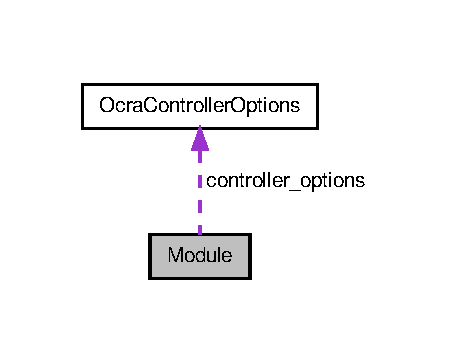
\includegraphics[width=216pt]{classModule__coll__graph}
\end{center}
\end{figure}
\subsection*{\-Public \-Member \-Functions}
\begin{DoxyCompactItemize}
\item 
\hyperlink{classModule_a5a240a8a9ab1813b17bcb810b24ceaea}{\-Module} ()
\item 
\hyperlink{classModule_a7c9d9c096786d127590fdd8aa2b7d681}{$\sim$\-Module} ()
\item 
bool \hyperlink{classModule_a1f18c762538086e1304ea18e00e51abb}{configure} (yarp\-::os\-::\-Resource\-Finder \&rf)
\item 
bool \hyperlink{classModule_ad53295be6c51e834eec92009c2d7bbf3}{interrupt\-Module} ()
\item 
bool \hyperlink{classModule_ab07583e4393148dfe0fd2ae6e7998a4b}{close} ()
\item 
bool \hyperlink{classModule_a1b1c4963512941537cef766217329a8a}{update\-Module} ()
\item 
void \hyperlink{classModule_a861f70d79b8f36dccf5daae182763bd8}{print\-Help} ()
\end{DoxyCompactItemize}
\subsection*{\-Private \-Attributes}
\begin{DoxyCompactItemize}
\item 
std\-::shared\-\_\-ptr$<$ \hyperlink{classThread}{\-Thread} $>$ \hyperlink{classModule_a39346aa2e2a00801e07f4c127ff004ba}{ctrl\-Thread}
\item 
std\-::shared\-\_\-ptr\*
$<$ wbi\-::whole\-Body\-Interface $>$ \hyperlink{classModule_a0d3efedabcef6ec0db88011ccc2e7205}{robot\-Interface}
\item 
yarp\-::os\-::\-Log \hyperlink{classModule_ae029b50069bf4ff53a6f69a5bae824f6}{y\-Log}
\item 
\hyperlink{classOcraControllerOptions}{\-Ocra\-Controller\-Options} \hyperlink{classModule_a04156183c6e15f118595e3637ab5372f}{controller\-\_\-options}
\item 
double \hyperlink{classModule_a1a20dbf0d18e5020ad85d38a0ba22b88}{avg\-Time}
\item 
double \hyperlink{classModule_af66a2dab82208cb2ea25da22fcaaa4a3}{std\-Dev}
\item 
double \hyperlink{classModule_a5baf8260eb8a45ebbb75474f2b277edc}{avg\-Time\-Used}
\item 
double \hyperlink{classModule_a57060f2788b6dc9906e66432e775e5ac}{std\-Dev\-Used}
\item 
double \hyperlink{classModule_a33fee1e7f977b4f27a2e1488480996fb}{danger\-Period\-Loop\-Time}
\end{DoxyCompactItemize}
\subsection*{\-Static \-Private \-Attributes}
\begin{DoxyCompactItemize}
\item 
static const int \hyperlink{classModule_af73cdfdae53c52ea8488d0d8c4f9083f}{\-D\-E\-F\-A\-U\-L\-T\-\_\-\-T\-H\-R\-E\-A\-D\-\_\-\-P\-E\-R\-I\-O\-D} = 10
\end{DoxyCompactItemize}


\subsection{\-Detailed \-Description}
\-The controller module which launches the controller thread. 

\-Basically all this does is parse the command line arguments and look for the various config and task set files. \-It then instantiates a \-W\-B\-I instance (yarp\-W\-B\-I specifically) and a \hyperlink{classThread}{\-Thread} instance. \-It launches these threads and then basically just waits till it gets a kill (ctrl+c) command to close them down. \-Does a little keeping track of time as well. 

\subsection{\-Constructor \& \-Destructor \-Documentation}
\hypertarget{classModule_a5a240a8a9ab1813b17bcb810b24ceaea}{\index{\-Module@{\-Module}!\-Module@{\-Module}}
\index{\-Module@{\-Module}!Module@{\-Module}}
\subsubsection[{\-Module}]{\setlength{\rightskip}{0pt plus 5cm}{\bf \-Module\-::\-Module} (
\begin{DoxyParamCaption}
{}
\end{DoxyParamCaption}
)}}\label{classModule_a5a240a8a9ab1813b17bcb810b24ceaea}
\-Constructor which essentially does nothing. \hypertarget{classModule_a7c9d9c096786d127590fdd8aa2b7d681}{\index{\-Module@{\-Module}!$\sim$\-Module@{$\sim$\-Module}}
\index{$\sim$\-Module@{$\sim$\-Module}!Module@{\-Module}}
\subsubsection[{$\sim$\-Module}]{\setlength{\rightskip}{0pt plus 5cm}{\bf \-Module\-::$\sim$\-Module} (
\begin{DoxyParamCaption}
{}
\end{DoxyParamCaption}
)}}\label{classModule_a7c9d9c096786d127590fdd8aa2b7d681}
\-Destructor which essentially does nothing. 

\subsection{\-Member \-Function \-Documentation}
\hypertarget{classModule_ab07583e4393148dfe0fd2ae6e7998a4b}{\index{\-Module@{\-Module}!close@{close}}
\index{close@{close}!Module@{\-Module}}
\subsubsection[{close}]{\setlength{\rightskip}{0pt plus 5cm}bool {\bf \-Module\-::close} (
\begin{DoxyParamCaption}
{}
\end{DoxyParamCaption}
)}}\label{classModule_ab07583e4393148dfe0fd2ae6e7998a4b}
\-Closes the module. \-First shuts down the threads. \hypertarget{classModule_a1f18c762538086e1304ea18e00e51abb}{\index{\-Module@{\-Module}!configure@{configure}}
\index{configure@{configure}!Module@{\-Module}}
\subsubsection[{configure}]{\setlength{\rightskip}{0pt plus 5cm}bool {\bf \-Module\-::configure} (
\begin{DoxyParamCaption}
\item[{yarp\-::os\-::\-Resource\-Finder \&}]{rf}
\end{DoxyParamCaption}
)}}\label{classModule_a1f18c762538086e1304ea18e00e51abb}
\-Configures the module by parsing the \-R\-F contents. 
\begin{DoxyParams}{\-Parameters}
{\em rf} & \-A resource finder instance which is initialized from the command line args.\\
\hline
\end{DoxyParams}
\begin{DoxyReturn}{\-Returns}
\-True or false if the configuration was successful. 
\end{DoxyReturn}
\hypertarget{classModule_ad53295be6c51e834eec92009c2d7bbf3}{\index{\-Module@{\-Module}!interrupt\-Module@{interrupt\-Module}}
\index{interrupt\-Module@{interrupt\-Module}!Module@{\-Module}}
\subsubsection[{interrupt\-Module}]{\setlength{\rightskip}{0pt plus 5cm}bool {\bf \-Module\-::interrupt\-Module} (
\begin{DoxyParamCaption}
{}
\end{DoxyParamCaption}
)}}\label{classModule_ad53295be6c51e834eec92009c2d7bbf3}
\-Interrupts the module execution and stops the control and wbi threads. \hypertarget{classModule_a861f70d79b8f36dccf5daae182763bd8}{\index{\-Module@{\-Module}!print\-Help@{print\-Help}}
\index{print\-Help@{print\-Help}!Module@{\-Module}}
\subsubsection[{print\-Help}]{\setlength{\rightskip}{0pt plus 5cm}void {\bf \-Module\-::print\-Help} (
\begin{DoxyParamCaption}
{}
\end{DoxyParamCaption}
)}}\label{classModule_a861f70d79b8f36dccf5daae182763bd8}
\-Prints all the command line args one could use. \hypertarget{classModule_a1b1c4963512941537cef766217329a8a}{\index{\-Module@{\-Module}!update\-Module@{update\-Module}}
\index{update\-Module@{update\-Module}!Module@{\-Module}}
\subsubsection[{update\-Module}]{\setlength{\rightskip}{0pt plus 5cm}bool {\bf \-Module\-::update\-Module} (
\begin{DoxyParamCaption}
{}
\end{DoxyParamCaption}
)}}\label{classModule_a1b1c4963512941537cef766217329a8a}
\-Updates the \hyperlink{classModule}{\-Module}. \-Basically just clocks the thread run() method. \begin{DoxyReturn}{\-Returns}
\-Whether or not the clocking functions worked. 
\end{DoxyReturn}


\subsection{\-Member \-Data \-Documentation}
\hypertarget{classModule_a1a20dbf0d18e5020ad85d38a0ba22b88}{\index{\-Module@{\-Module}!avg\-Time@{avg\-Time}}
\index{avg\-Time@{avg\-Time}!Module@{\-Module}}
\subsubsection[{avg\-Time}]{\setlength{\rightskip}{0pt plus 5cm}double {\bf \-Module\-::avg\-Time}\hspace{0.3cm}{\ttfamily  \mbox{[}private\mbox{]}}}}\label{classModule_a1a20dbf0d18e5020ad85d38a0ba22b88}
\-Average time between successive calls of the `run()` method. \hypertarget{classModule_a5baf8260eb8a45ebbb75474f2b277edc}{\index{\-Module@{\-Module}!avg\-Time\-Used@{avg\-Time\-Used}}
\index{avg\-Time\-Used@{avg\-Time\-Used}!Module@{\-Module}}
\subsubsection[{avg\-Time\-Used}]{\setlength{\rightskip}{0pt plus 5cm}double {\bf \-Module\-::avg\-Time\-Used}\hspace{0.3cm}{\ttfamily  \mbox{[}private\mbox{]}}}}\label{classModule_a5baf8260eb8a45ebbb75474f2b277edc}
\-Average time for the `run()` method to execute. \-Should be close to avg\-Time. \hypertarget{classModule_a04156183c6e15f118595e3637ab5372f}{\index{\-Module@{\-Module}!controller\-\_\-options@{controller\-\_\-options}}
\index{controller\-\_\-options@{controller\-\_\-options}!Module@{\-Module}}
\subsubsection[{controller\-\_\-options}]{\setlength{\rightskip}{0pt plus 5cm}{\bf \-Ocra\-Controller\-Options} {\bf \-Module\-::controller\-\_\-options}\hspace{0.3cm}{\ttfamily  \mbox{[}private\mbox{]}}}}\label{classModule_a04156183c6e15f118595e3637ab5372f}
\-Options used for the controller. \hypertarget{classModule_a39346aa2e2a00801e07f4c127ff004ba}{\index{\-Module@{\-Module}!ctrl\-Thread@{ctrl\-Thread}}
\index{ctrl\-Thread@{ctrl\-Thread}!Module@{\-Module}}
\subsubsection[{ctrl\-Thread}]{\setlength{\rightskip}{0pt plus 5cm}std\-::shared\-\_\-ptr$<${\bf \-Thread}$>$ {\bf \-Module\-::ctrl\-Thread}\hspace{0.3cm}{\ttfamily  \mbox{[}private\mbox{]}}}}\label{classModule_a39346aa2e2a00801e07f4c127ff004ba}
\-The controller thread. \-This is where the magic happens. \hypertarget{classModule_a33fee1e7f977b4f27a2e1488480996fb}{\index{\-Module@{\-Module}!danger\-Period\-Loop\-Time@{danger\-Period\-Loop\-Time}}
\index{danger\-Period\-Loop\-Time@{danger\-Period\-Loop\-Time}!Module@{\-Module}}
\subsubsection[{danger\-Period\-Loop\-Time}]{\setlength{\rightskip}{0pt plus 5cm}double {\bf \-Module\-::danger\-Period\-Loop\-Time}\hspace{0.3cm}{\ttfamily  \mbox{[}private\mbox{]}}}}\label{classModule_a33fee1e7f977b4f27a2e1488480996fb}
\-A value which the thread period loop time should not exceed. \hypertarget{classModule_af73cdfdae53c52ea8488d0d8c4f9083f}{\index{\-Module@{\-Module}!\-D\-E\-F\-A\-U\-L\-T\-\_\-\-T\-H\-R\-E\-A\-D\-\_\-\-P\-E\-R\-I\-O\-D@{\-D\-E\-F\-A\-U\-L\-T\-\_\-\-T\-H\-R\-E\-A\-D\-\_\-\-P\-E\-R\-I\-O\-D}}
\index{\-D\-E\-F\-A\-U\-L\-T\-\_\-\-T\-H\-R\-E\-A\-D\-\_\-\-P\-E\-R\-I\-O\-D@{\-D\-E\-F\-A\-U\-L\-T\-\_\-\-T\-H\-R\-E\-A\-D\-\_\-\-P\-E\-R\-I\-O\-D}!Module@{\-Module}}
\subsubsection[{\-D\-E\-F\-A\-U\-L\-T\-\_\-\-T\-H\-R\-E\-A\-D\-\_\-\-P\-E\-R\-I\-O\-D}]{\setlength{\rightskip}{0pt plus 5cm}const int {\bf \-Module\-::\-D\-E\-F\-A\-U\-L\-T\-\_\-\-T\-H\-R\-E\-A\-D\-\_\-\-P\-E\-R\-I\-O\-D} = 10\hspace{0.3cm}{\ttfamily  \mbox{[}static, private\mbox{]}}}}\label{classModule_af73cdfdae53c52ea8488d0d8c4f9083f}
\-If the user doesn't provide a thread period make it 10ms. \hypertarget{classModule_a0d3efedabcef6ec0db88011ccc2e7205}{\index{\-Module@{\-Module}!robot\-Interface@{robot\-Interface}}
\index{robot\-Interface@{robot\-Interface}!Module@{\-Module}}
\subsubsection[{robot\-Interface}]{\setlength{\rightskip}{0pt plus 5cm}std\-::shared\-\_\-ptr$<$wbi\-::whole\-Body\-Interface$>$ {\bf \-Module\-::robot\-Interface}\hspace{0.3cm}{\ttfamily  \mbox{[}private\mbox{]}}}}\label{classModule_a0d3efedabcef6ec0db88011ccc2e7205}
\-The yarp\-W\-B\-I interface used to get estimates from the robot. \hypertarget{classModule_af66a2dab82208cb2ea25da22fcaaa4a3}{\index{\-Module@{\-Module}!std\-Dev@{std\-Dev}}
\index{std\-Dev@{std\-Dev}!Module@{\-Module}}
\subsubsection[{std\-Dev}]{\setlength{\rightskip}{0pt plus 5cm}double {\bf \-Module\-::std\-Dev}\hspace{0.3cm}{\ttfamily  \mbox{[}private\mbox{]}}}}\label{classModule_af66a2dab82208cb2ea25da22fcaaa4a3}
\-Standard deviation of the average time between successive calls of the `run()` method. \hypertarget{classModule_a57060f2788b6dc9906e66432e775e5ac}{\index{\-Module@{\-Module}!std\-Dev\-Used@{std\-Dev\-Used}}
\index{std\-Dev\-Used@{std\-Dev\-Used}!Module@{\-Module}}
\subsubsection[{std\-Dev\-Used}]{\setlength{\rightskip}{0pt plus 5cm}double {\bf \-Module\-::std\-Dev\-Used}\hspace{0.3cm}{\ttfamily  \mbox{[}private\mbox{]}}}}\label{classModule_a57060f2788b6dc9906e66432e775e5ac}
\-Standard deviation of the average time for the `run()` method to execute. \hypertarget{classModule_ae029b50069bf4ff53a6f69a5bae824f6}{\index{\-Module@{\-Module}!y\-Log@{y\-Log}}
\index{y\-Log@{y\-Log}!Module@{\-Module}}
\subsubsection[{y\-Log}]{\setlength{\rightskip}{0pt plus 5cm}yarp\-::os\-::\-Log {\bf \-Module\-::y\-Log}\hspace{0.3cm}{\ttfamily  \mbox{[}private\mbox{]}}}}\label{classModule_ae029b50069bf4ff53a6f69a5bae824f6}
\-A yarp logging tool. 

\-The documentation for this class was generated from the following files\-:\begin{DoxyCompactItemize}
\item 
ocra-\/wbi-\/plugins/ocra-\/icub-\/server/include/ocra-\/icub-\/server/\hyperlink{Module_8h}{\-Module.\-h}\item 
ocra-\/wbi-\/plugins/ocra-\/icub-\/server/src/\hyperlink{Module_8cpp}{\-Module.\-cpp}\end{DoxyCompactItemize}

\hypertarget{classOcraControllerOptions}{\section{\-Ocra\-Controller\-Options \-Class \-Reference}
\label{classOcraControllerOptions}\index{\-Ocra\-Controller\-Options@{\-Ocra\-Controller\-Options}}
}


{\ttfamily \#include $<$\-Thread.\-h$>$}

\subsection*{\-Public \-Member \-Functions}
\begin{DoxyCompactItemize}
\item 
\hyperlink{classOcraControllerOptions_a1a91de992c42c6da488e95cd594eca80}{\-Ocra\-Controller\-Options} ()
\item 
\hyperlink{classOcraControllerOptions_a22f514e92ccf91cc362c48a6c340ac19}{$\sim$\-Ocra\-Controller\-Options} ()
\end{DoxyCompactItemize}
\subsection*{\-Public \-Attributes}
\begin{DoxyCompactItemize}
\item 
int \hyperlink{classOcraControllerOptions_ab706ae593bf5b30433cfd6f957b51db4}{thread\-Period}
\item 
std\-::string \hyperlink{classOcraControllerOptions_a22380b083fbf0b202993d0415d1d4c83}{server\-Name}
\item 
std\-::string \hyperlink{classOcraControllerOptions_a897948011f23b08ba20e1707033458d4}{robot\-Name}
\item 
std\-::string \hyperlink{classOcraControllerOptions_af91566ecff3f7ed02571369c7af061ce}{startup\-Task\-Set\-Path}
\item 
std\-::string \hyperlink{classOcraControllerOptions_ab01efbd786ad8bc5beb6de02dbcd0936}{startup\-Sequence}
\item 
std\-::string \hyperlink{classOcraControllerOptions_af3a98210531cf667c2838e45b470a66e}{wbi\-Config\-File\-Path}
\item 
std\-::string \hyperlink{classOcraControllerOptions_a697196e6267b2a519dd0bcc2bc03ab73}{urdf\-Model\-Path}
\item 
bool \hyperlink{classOcraControllerOptions_a26dce90c0e6cf7ba608020d01cd08f3c}{run\-In\-Debug\-Mode}
\item 
bool \hyperlink{classOcraControllerOptions_af05db2783f36f469fa535fd4ba5c12b1}{no\-Output\-Mode}
\item 
bool \hyperlink{classOcraControllerOptions_a1edf322553d88c1ac2bf8947e9d942d7}{is\-Floating\-Base}
\item 
bool \hyperlink{classOcraControllerOptions_a335f09b446b6d10e2a8e6eb453391d9e}{use\-Odometry}
\item 
bool \hyperlink{classOcraControllerOptions_a34c0a162302f4f2c462d9ce4818292d5}{idle\-Ankles}
\item 
double \hyperlink{classOcraControllerOptions_af09053d38fbafe448a35804ea86d27aa}{idle\-Ankle\-Time}
\item 
bool \hyperlink{classOcraControllerOptions_ae7b16a5b8264abd18ee8761eb1091ccf}{maintain\-Final\-Posture}
\item 
yarp\-::os\-::\-Property \hyperlink{classOcraControllerOptions_ac3965bdcce6cb2ce3e4a335f855acd63}{yarp\-Wbi\-Options}
\item 
ocra\-\_\-recipes\-::\-C\-O\-N\-T\-R\-O\-L\-L\-E\-R\-\_\-\-T\-Y\-P\-E \hyperlink{classOcraControllerOptions_aa533fe11c53b7fb17105f1edf48e1c0d}{controller\-Type}
\item 
ocra\-\_\-recipes\-::\-S\-O\-L\-V\-E\-R\-\_\-\-T\-Y\-P\-E \hyperlink{classOcraControllerOptions_af79b8705c3f3097b642262bc877eaa8e}{solver}
\item 
double \hyperlink{classOcraControllerOptions_aab63ca12dec23284464b978c4e3e1c62}{w\-Ddq}
\item 
double \hyperlink{classOcraControllerOptions_ada37aedbe3639334803637b55c650bc0}{w\-Tau}
\item 
double \hyperlink{classOcraControllerOptions_a96706a52ac56f2598d03e80c9c778ce7}{w\-Fc}
\end{DoxyCompactItemize}


\subsection{\-Constructor \& \-Destructor \-Documentation}
\hypertarget{classOcraControllerOptions_a1a91de992c42c6da488e95cd594eca80}{\index{\-Ocra\-Controller\-Options@{\-Ocra\-Controller\-Options}!\-Ocra\-Controller\-Options@{\-Ocra\-Controller\-Options}}
\index{\-Ocra\-Controller\-Options@{\-Ocra\-Controller\-Options}!OcraControllerOptions@{\-Ocra\-Controller\-Options}}
\subsubsection[{\-Ocra\-Controller\-Options}]{\setlength{\rightskip}{0pt plus 5cm}{\bf \-Ocra\-Controller\-Options\-::\-Ocra\-Controller\-Options} (
\begin{DoxyParamCaption}
{}
\end{DoxyParamCaption}
)}}\label{classOcraControllerOptions_a1a91de992c42c6da488e95cd594eca80}
\-Constructor. \-Initializes all of the possible values. \hypertarget{classOcraControllerOptions_a22f514e92ccf91cc362c48a6c340ac19}{\index{\-Ocra\-Controller\-Options@{\-Ocra\-Controller\-Options}!$\sim$\-Ocra\-Controller\-Options@{$\sim$\-Ocra\-Controller\-Options}}
\index{$\sim$\-Ocra\-Controller\-Options@{$\sim$\-Ocra\-Controller\-Options}!OcraControllerOptions@{\-Ocra\-Controller\-Options}}
\subsubsection[{$\sim$\-Ocra\-Controller\-Options}]{\setlength{\rightskip}{0pt plus 5cm}{\bf \-Ocra\-Controller\-Options\-::$\sim$\-Ocra\-Controller\-Options} (
\begin{DoxyParamCaption}
{}
\end{DoxyParamCaption}
)}}\label{classOcraControllerOptions_a22f514e92ccf91cc362c48a6c340ac19}
\-Destructor. \-Does nothing. 

\subsection{\-Member \-Data \-Documentation}
\hypertarget{classOcraControllerOptions_aa533fe11c53b7fb17105f1edf48e1c0d}{\index{\-Ocra\-Controller\-Options@{\-Ocra\-Controller\-Options}!controller\-Type@{controller\-Type}}
\index{controller\-Type@{controller\-Type}!OcraControllerOptions@{\-Ocra\-Controller\-Options}}
\subsubsection[{controller\-Type}]{\setlength{\rightskip}{0pt plus 5cm}ocra\-\_\-recipes\-::\-C\-O\-N\-T\-R\-O\-L\-L\-E\-R\-\_\-\-T\-Y\-P\-E {\bf \-Ocra\-Controller\-Options\-::controller\-Type}}}\label{classOcraControllerOptions_aa533fe11c53b7fb17105f1edf48e1c0d}
\-The type of \-O\-C\-R\-A controller to use. \hypertarget{classOcraControllerOptions_a34c0a162302f4f2c462d9ce4818292d5}{\index{\-Ocra\-Controller\-Options@{\-Ocra\-Controller\-Options}!idle\-Ankles@{idle\-Ankles}}
\index{idle\-Ankles@{idle\-Ankles}!OcraControllerOptions@{\-Ocra\-Controller\-Options}}
\subsubsection[{idle\-Ankles}]{\setlength{\rightskip}{0pt plus 5cm}bool {\bf \-Ocra\-Controller\-Options\-::idle\-Ankles}}}\label{classOcraControllerOptions_a34c0a162302f4f2c462d9ce4818292d5}
\-A boolean which tells the controller to idle the ankles for a short period and then pass on to normal operation. \-This is to get the feet flush with the ground. \hypertarget{classOcraControllerOptions_af09053d38fbafe448a35804ea86d27aa}{\index{\-Ocra\-Controller\-Options@{\-Ocra\-Controller\-Options}!idle\-Ankle\-Time@{idle\-Ankle\-Time}}
\index{idle\-Ankle\-Time@{idle\-Ankle\-Time}!OcraControllerOptions@{\-Ocra\-Controller\-Options}}
\subsubsection[{idle\-Ankle\-Time}]{\setlength{\rightskip}{0pt plus 5cm}double {\bf \-Ocra\-Controller\-Options\-::idle\-Ankle\-Time}}}\label{classOcraControllerOptions_af09053d38fbafe448a35804ea86d27aa}
\-Number of seconds to idle the ankle. \-By default 1.\-5s. \hypertarget{classOcraControllerOptions_a1edf322553d88c1ac2bf8947e9d942d7}{\index{\-Ocra\-Controller\-Options@{\-Ocra\-Controller\-Options}!is\-Floating\-Base@{is\-Floating\-Base}}
\index{is\-Floating\-Base@{is\-Floating\-Base}!OcraControllerOptions@{\-Ocra\-Controller\-Options}}
\subsubsection[{is\-Floating\-Base}]{\setlength{\rightskip}{0pt plus 5cm}bool {\bf \-Ocra\-Controller\-Options\-::is\-Floating\-Base}}}\label{classOcraControllerOptions_a1edf322553d88c1ac2bf8947e9d942d7}
a boolean which tells the controller whether the robot has a fixed or floating base. \hypertarget{classOcraControllerOptions_ae7b16a5b8264abd18ee8761eb1091ccf}{\index{\-Ocra\-Controller\-Options@{\-Ocra\-Controller\-Options}!maintain\-Final\-Posture@{maintain\-Final\-Posture}}
\index{maintain\-Final\-Posture@{maintain\-Final\-Posture}!OcraControllerOptions@{\-Ocra\-Controller\-Options}}
\subsubsection[{maintain\-Final\-Posture}]{\setlength{\rightskip}{0pt plus 5cm}bool {\bf \-Ocra\-Controller\-Options\-::maintain\-Final\-Posture}}}\label{classOcraControllerOptions_ae7b16a5b8264abd18ee8761eb1091ccf}
\-A boolean which tells the controller to stay in its final posture when the controller is switched to position mode at the end of usage. \hypertarget{classOcraControllerOptions_af05db2783f36f469fa535fd4ba5c12b1}{\index{\-Ocra\-Controller\-Options@{\-Ocra\-Controller\-Options}!no\-Output\-Mode@{no\-Output\-Mode}}
\index{no\-Output\-Mode@{no\-Output\-Mode}!OcraControllerOptions@{\-Ocra\-Controller\-Options}}
\subsubsection[{no\-Output\-Mode}]{\setlength{\rightskip}{0pt plus 5cm}bool {\bf \-Ocra\-Controller\-Options\-::no\-Output\-Mode}}}\label{classOcraControllerOptions_af05db2783f36f469fa535fd4ba5c12b1}
a boolean which runs the controller in a debugging mode but never sends the torques to the robot. \hypertarget{classOcraControllerOptions_a897948011f23b08ba20e1707033458d4}{\index{\-Ocra\-Controller\-Options@{\-Ocra\-Controller\-Options}!robot\-Name@{robot\-Name}}
\index{robot\-Name@{robot\-Name}!OcraControllerOptions@{\-Ocra\-Controller\-Options}}
\subsubsection[{robot\-Name}]{\setlength{\rightskip}{0pt plus 5cm}std\-::string {\bf \-Ocra\-Controller\-Options\-::robot\-Name}}}\label{classOcraControllerOptions_a897948011f23b08ba20e1707033458d4}
a string with the name of the robot. \hypertarget{classOcraControllerOptions_a26dce90c0e6cf7ba608020d01cd08f3c}{\index{\-Ocra\-Controller\-Options@{\-Ocra\-Controller\-Options}!run\-In\-Debug\-Mode@{run\-In\-Debug\-Mode}}
\index{run\-In\-Debug\-Mode@{run\-In\-Debug\-Mode}!OcraControllerOptions@{\-Ocra\-Controller\-Options}}
\subsubsection[{run\-In\-Debug\-Mode}]{\setlength{\rightskip}{0pt plus 5cm}bool {\bf \-Ocra\-Controller\-Options\-::run\-In\-Debug\-Mode}}}\label{classOcraControllerOptions_a26dce90c0e6cf7ba608020d01cd08f3c}
a boolean which runs the controller in a debugging mode which allows one to check the controller ouput joint by joint. \hypertarget{classOcraControllerOptions_a22380b083fbf0b202993d0415d1d4c83}{\index{\-Ocra\-Controller\-Options@{\-Ocra\-Controller\-Options}!server\-Name@{server\-Name}}
\index{server\-Name@{server\-Name}!OcraControllerOptions@{\-Ocra\-Controller\-Options}}
\subsubsection[{server\-Name}]{\setlength{\rightskip}{0pt plus 5cm}std\-::string {\bf \-Ocra\-Controller\-Options\-::server\-Name}}}\label{classOcraControllerOptions_a22380b083fbf0b202993d0415d1d4c83}
a string with the name of the controller server. \hypertarget{classOcraControllerOptions_af79b8705c3f3097b642262bc877eaa8e}{\index{\-Ocra\-Controller\-Options@{\-Ocra\-Controller\-Options}!solver@{solver}}
\index{solver@{solver}!OcraControllerOptions@{\-Ocra\-Controller\-Options}}
\subsubsection[{solver}]{\setlength{\rightskip}{0pt plus 5cm}ocra\-\_\-recipes\-::\-S\-O\-L\-V\-E\-R\-\_\-\-T\-Y\-P\-E {\bf \-Ocra\-Controller\-Options\-::solver}}}\label{classOcraControllerOptions_af79b8705c3f3097b642262bc877eaa8e}
\-The type of \-O\-C\-R\-A controller to use. \hypertarget{classOcraControllerOptions_ab01efbd786ad8bc5beb6de02dbcd0936}{\index{\-Ocra\-Controller\-Options@{\-Ocra\-Controller\-Options}!startup\-Sequence@{startup\-Sequence}}
\index{startup\-Sequence@{startup\-Sequence}!OcraControllerOptions@{\-Ocra\-Controller\-Options}}
\subsubsection[{startup\-Sequence}]{\setlength{\rightskip}{0pt plus 5cm}std\-::string {\bf \-Ocra\-Controller\-Options\-::startup\-Sequence}}}\label{classOcraControllerOptions_ab01efbd786ad8bc5beb6de02dbcd0936}
a string with the name of a sequence to run $\ast$$\ast$(will be removed)$\ast$$\ast$. \hypertarget{classOcraControllerOptions_af91566ecff3f7ed02571369c7af061ce}{\index{\-Ocra\-Controller\-Options@{\-Ocra\-Controller\-Options}!startup\-Task\-Set\-Path@{startup\-Task\-Set\-Path}}
\index{startup\-Task\-Set\-Path@{startup\-Task\-Set\-Path}!OcraControllerOptions@{\-Ocra\-Controller\-Options}}
\subsubsection[{startup\-Task\-Set\-Path}]{\setlength{\rightskip}{0pt plus 5cm}std\-::string {\bf \-Ocra\-Controller\-Options\-::startup\-Task\-Set\-Path}}}\label{classOcraControllerOptions_af91566ecff3f7ed02571369c7af061ce}
a string with the absolute path to an xml file with a set of tasks. \hypertarget{classOcraControllerOptions_ab706ae593bf5b30433cfd6f957b51db4}{\index{\-Ocra\-Controller\-Options@{\-Ocra\-Controller\-Options}!thread\-Period@{thread\-Period}}
\index{thread\-Period@{thread\-Period}!OcraControllerOptions@{\-Ocra\-Controller\-Options}}
\subsubsection[{thread\-Period}]{\setlength{\rightskip}{0pt plus 5cm}int {\bf \-Ocra\-Controller\-Options\-::thread\-Period}}}\label{classOcraControllerOptions_ab706ae593bf5b30433cfd6f957b51db4}
\-An int representing the looping period of the controller. \hypertarget{classOcraControllerOptions_a697196e6267b2a519dd0bcc2bc03ab73}{\index{\-Ocra\-Controller\-Options@{\-Ocra\-Controller\-Options}!urdf\-Model\-Path@{urdf\-Model\-Path}}
\index{urdf\-Model\-Path@{urdf\-Model\-Path}!OcraControllerOptions@{\-Ocra\-Controller\-Options}}
\subsubsection[{urdf\-Model\-Path}]{\setlength{\rightskip}{0pt plus 5cm}std\-::string {\bf \-Ocra\-Controller\-Options\-::urdf\-Model\-Path}}}\label{classOcraControllerOptions_a697196e6267b2a519dd0bcc2bc03ab73}
\-Absolute path to the urdf model. \-Used for the odometry. \hypertarget{classOcraControllerOptions_a335f09b446b6d10e2a8e6eb453391d9e}{\index{\-Ocra\-Controller\-Options@{\-Ocra\-Controller\-Options}!use\-Odometry@{use\-Odometry}}
\index{use\-Odometry@{use\-Odometry}!OcraControllerOptions@{\-Ocra\-Controller\-Options}}
\subsubsection[{use\-Odometry}]{\setlength{\rightskip}{0pt plus 5cm}bool {\bf \-Ocra\-Controller\-Options\-::use\-Odometry}}}\label{classOcraControllerOptions_a335f09b446b6d10e2a8e6eb453391d9e}
a boolean which tells the controller to start the odometry, meaning that the world reference frame remains attached to the ground \hypertarget{classOcraControllerOptions_af3a98210531cf667c2838e45b470a66e}{\index{\-Ocra\-Controller\-Options@{\-Ocra\-Controller\-Options}!wbi\-Config\-File\-Path@{wbi\-Config\-File\-Path}}
\index{wbi\-Config\-File\-Path@{wbi\-Config\-File\-Path}!OcraControllerOptions@{\-Ocra\-Controller\-Options}}
\subsubsection[{wbi\-Config\-File\-Path}]{\setlength{\rightskip}{0pt plus 5cm}std\-::string {\bf \-Ocra\-Controller\-Options\-::wbi\-Config\-File\-Path}}}\label{classOcraControllerOptions_af3a98210531cf667c2838e45b470a66e}
\-The absolute path to the configuration file used to initialize the yarp\-W\-B\-I. \hypertarget{classOcraControllerOptions_aab63ca12dec23284464b978c4e3e1c62}{\index{\-Ocra\-Controller\-Options@{\-Ocra\-Controller\-Options}!w\-Ddq@{w\-Ddq}}
\index{w\-Ddq@{w\-Ddq}!OcraControllerOptions@{\-Ocra\-Controller\-Options}}
\subsubsection[{w\-Ddq}]{\setlength{\rightskip}{0pt plus 5cm}double {\bf \-Ocra\-Controller\-Options\-::w\-Ddq}}}\label{classOcraControllerOptions_aab63ca12dec23284464b978c4e3e1c62}
\hypertarget{classOcraControllerOptions_a96706a52ac56f2598d03e80c9c778ce7}{\index{\-Ocra\-Controller\-Options@{\-Ocra\-Controller\-Options}!w\-Fc@{w\-Fc}}
\index{w\-Fc@{w\-Fc}!OcraControllerOptions@{\-Ocra\-Controller\-Options}}
\subsubsection[{w\-Fc}]{\setlength{\rightskip}{0pt plus 5cm}double {\bf \-Ocra\-Controller\-Options\-::w\-Fc}}}\label{classOcraControllerOptions_a96706a52ac56f2598d03e80c9c778ce7}
\hypertarget{classOcraControllerOptions_ada37aedbe3639334803637b55c650bc0}{\index{\-Ocra\-Controller\-Options@{\-Ocra\-Controller\-Options}!w\-Tau@{w\-Tau}}
\index{w\-Tau@{w\-Tau}!OcraControllerOptions@{\-Ocra\-Controller\-Options}}
\subsubsection[{w\-Tau}]{\setlength{\rightskip}{0pt plus 5cm}double {\bf \-Ocra\-Controller\-Options\-::w\-Tau}}}\label{classOcraControllerOptions_ada37aedbe3639334803637b55c650bc0}
\hypertarget{classOcraControllerOptions_ac3965bdcce6cb2ce3e4a335f855acd63}{\index{\-Ocra\-Controller\-Options@{\-Ocra\-Controller\-Options}!yarp\-Wbi\-Options@{yarp\-Wbi\-Options}}
\index{yarp\-Wbi\-Options@{yarp\-Wbi\-Options}!OcraControllerOptions@{\-Ocra\-Controller\-Options}}
\subsubsection[{yarp\-Wbi\-Options}]{\setlength{\rightskip}{0pt plus 5cm}yarp\-::os\-::\-Property {\bf \-Ocra\-Controller\-Options\-::yarp\-Wbi\-Options}}}\label{classOcraControllerOptions_ac3965bdcce6cb2ce3e4a335f855acd63}
\-Options for the \-W\-B\-I used to update the model. 

\-The documentation for this class was generated from the following files\-:\begin{DoxyCompactItemize}
\item 
ocra-\/wbi-\/plugins/ocra-\/icub-\/server/include/ocra-\/icub-\/server/\hyperlink{Thread_8h}{\-Thread.\-h}\item 
ocra-\/wbi-\/plugins/ocra-\/icub-\/server/src/\hyperlink{Thread_8cpp}{\-Thread.\-cpp}\end{DoxyCompactItemize}

\hypertarget{classocra__icub_1_1OcraWbiConversions}{\section{ocra\-\_\-icub\-:\-:\-Ocra\-Wbi\-Conversions \-Class \-Reference}
\label{classocra__icub_1_1OcraWbiConversions}\index{ocra\-\_\-icub\-::\-Ocra\-Wbi\-Conversions@{ocra\-\_\-icub\-::\-Ocra\-Wbi\-Conversions}}
}


{\ttfamily \#include $<$\-Ocra\-Wbi\-Conversions.\-h$>$}

\subsection*{\-Static \-Public \-Member \-Functions}
\begin{DoxyCompactItemize}
\item 
static bool \hyperlink{classocra__icub_1_1OcraWbiConversions_af71562a5f3d4f6e649f1cec0a3d9996b}{eigen\-Dispd\-To\-Wbi\-Frame} (const \-Eigen\-::\-Displacementd \&disp, wbi\-::\-Frame \&frame)
\item 
static bool \hyperlink{classocra__icub_1_1OcraWbiConversions_a403627efa183c8ddbbccabf0dcd5bcaf}{wbi\-Frame\-To\-Eigen\-Dispd} (const wbi\-::\-Frame \&frame, \-Eigen\-::\-Displacementd \&disp)
\item 
static bool \hyperlink{classocra__icub_1_1OcraWbiConversions_a37c2aea3bf156928cb90a16655c24cc9}{wbi\-To\-Ocra\-Twist\-Vector} (\-Eigen\-::\-Twistd \&t\-\_\-wbi, \-Eigen\-::\-Twistd \&t\-\_\-ocra)
\item 
static bool \hyperlink{classocra__icub_1_1OcraWbiConversions_a7725aea95eb71c805def4a064a2693fa}{ocra\-To\-Wbi\-Twist\-Vector} (\-Eigen\-::\-Twistd \&t\-\_\-ocra, \-Eigen\-::\-Twistd \&t\-\_\-wbi)
\item 
static bool \hyperlink{classocra__icub_1_1OcraWbiConversions_a25a64172ebb14db9ddf301880a433964}{wbi\-To\-Ocra\-Seg\-Jacobian} (const \-Eigen\-::\-Matrix\-Xd \&jac, \-Eigen\-::\-Matrix\-Xd \&\-J)
\item 
static bool \hyperlink{classocra__icub_1_1OcraWbiConversions_a86458de950caa3bde3aa1d1aff448be1}{wbi\-To\-Ocra\-Co\-M\-Jacobian} (const \-Eigen\-::\-Matrix\-Xd \&jac, \-Eigen\-::\-Matrix$<$ double, 3, \-Eigen\-::\-Dynamic $>$ \&\-J)
\item 
static bool \hyperlink{classocra__icub_1_1OcraWbiConversions_ac03ed9581c49479b3ade94d58a3295b4}{eigen\-Row\-Major\-To\-Col\-Major} (const \hyperlink{namespaceocra__icub_aa5e36a19ed031c28ca83c207bd7dd83f}{\-Matrix\-Xd\-Rm} \&\-M\-\_\-rm, \-Eigen\-::\-Matrix\-Xd \&\-M)
\item 
static bool \hyperlink{classocra__icub_1_1OcraWbiConversions_abaa2b7a9069b60cfb36cb21e89b98177}{wbi\-To\-Ocra\-Mass\-Matrix} (int qdof, const \-Eigen\-::\-Matrix\-Xd \&\-M\-\_\-wbi, \-Eigen\-::\-Matrix\-Xd \&\-M\-\_\-ocra)
\item 
static bool \hyperlink{classocra__icub_1_1OcraWbiConversions_ae8839dfdc97e2239f4ed8a257d32fb21}{wbi\-To\-Ocra\-Body\-Vector} (int qdof, const \-Eigen\-::\-Vector\-Xd \&v\-\_\-wbi, \-Eigen\-::\-Vector\-Xd \&v\-\_\-ocra)
\item 
static bool \hyperlink{classocra__icub_1_1OcraWbiConversions_a1197be5b35329fbec85de8ee3c4abbd5}{eigen\-To\-Yarp\-Vector} (const \-Eigen\-::\-Vector\-Xd \&eigen\-Vector, yarp\-::sig\-::\-Vector \&yarp\-Vector)
\end{DoxyCompactItemize}
\subsection*{\-Static \-Public \-Attributes}
\begin{DoxyCompactItemize}
\item 
static const int \hyperlink{classocra__icub_1_1OcraWbiConversions_a7c628bd1208c5e70be458d4dffda4d06}{\-D\-I\-M\-\_\-\-T\-R\-A\-N\-S\-L\-A\-T\-I\-O\-N} = 3
\item 
static const int \hyperlink{classocra__icub_1_1OcraWbiConversions_a05e66392df58e9dda2d4db590bdd65a0}{\-D\-I\-M\-\_\-\-R\-O\-T\-A\-T\-I\-O\-N} = 3
\end{DoxyCompactItemize}


\subsection{\-Member \-Function \-Documentation}
\hypertarget{classocra__icub_1_1OcraWbiConversions_af71562a5f3d4f6e649f1cec0a3d9996b}{\index{ocra\-\_\-icub\-::\-Ocra\-Wbi\-Conversions@{ocra\-\_\-icub\-::\-Ocra\-Wbi\-Conversions}!eigen\-Dispd\-To\-Wbi\-Frame@{eigen\-Dispd\-To\-Wbi\-Frame}}
\index{eigen\-Dispd\-To\-Wbi\-Frame@{eigen\-Dispd\-To\-Wbi\-Frame}!ocra_icub::OcraWbiConversions@{ocra\-\_\-icub\-::\-Ocra\-Wbi\-Conversions}}
\subsubsection[{eigen\-Dispd\-To\-Wbi\-Frame}]{\setlength{\rightskip}{0pt plus 5cm}bool {\bf \-Ocra\-Wbi\-Conversions\-::eigen\-Dispd\-To\-Wbi\-Frame} (
\begin{DoxyParamCaption}
\item[{const \-Eigen\-::\-Displacementd \&}]{disp, }
\item[{wbi\-::\-Frame \&}]{frame}
\end{DoxyParamCaption}
)\hspace{0.3cm}{\ttfamily  \mbox{[}static\mbox{]}}}}\label{classocra__icub_1_1OcraWbiConversions_af71562a5f3d4f6e649f1cec0a3d9996b}
\hypertarget{classocra__icub_1_1OcraWbiConversions_ac03ed9581c49479b3ade94d58a3295b4}{\index{ocra\-\_\-icub\-::\-Ocra\-Wbi\-Conversions@{ocra\-\_\-icub\-::\-Ocra\-Wbi\-Conversions}!eigen\-Row\-Major\-To\-Col\-Major@{eigen\-Row\-Major\-To\-Col\-Major}}
\index{eigen\-Row\-Major\-To\-Col\-Major@{eigen\-Row\-Major\-To\-Col\-Major}!ocra_icub::OcraWbiConversions@{ocra\-\_\-icub\-::\-Ocra\-Wbi\-Conversions}}
\subsubsection[{eigen\-Row\-Major\-To\-Col\-Major}]{\setlength{\rightskip}{0pt plus 5cm}bool {\bf \-Ocra\-Wbi\-Conversions\-::eigen\-Row\-Major\-To\-Col\-Major} (
\begin{DoxyParamCaption}
\item[{const {\bf \-Matrix\-Xd\-Rm} \&}]{\-M\-\_\-rm, }
\item[{\-Eigen\-::\-Matrix\-Xd \&}]{\-M}
\end{DoxyParamCaption}
)\hspace{0.3cm}{\ttfamily  \mbox{[}static\mbox{]}}}}\label{classocra__icub_1_1OcraWbiConversions_ac03ed9581c49479b3ade94d58a3295b4}
\hypertarget{classocra__icub_1_1OcraWbiConversions_a1197be5b35329fbec85de8ee3c4abbd5}{\index{ocra\-\_\-icub\-::\-Ocra\-Wbi\-Conversions@{ocra\-\_\-icub\-::\-Ocra\-Wbi\-Conversions}!eigen\-To\-Yarp\-Vector@{eigen\-To\-Yarp\-Vector}}
\index{eigen\-To\-Yarp\-Vector@{eigen\-To\-Yarp\-Vector}!ocra_icub::OcraWbiConversions@{ocra\-\_\-icub\-::\-Ocra\-Wbi\-Conversions}}
\subsubsection[{eigen\-To\-Yarp\-Vector}]{\setlength{\rightskip}{0pt plus 5cm}bool {\bf \-Ocra\-Wbi\-Conversions\-::eigen\-To\-Yarp\-Vector} (
\begin{DoxyParamCaption}
\item[{const \-Eigen\-::\-Vector\-Xd \&}]{eigen\-Vector, }
\item[{yarp\-::sig\-::\-Vector \&}]{yarp\-Vector}
\end{DoxyParamCaption}
)\hspace{0.3cm}{\ttfamily  \mbox{[}static\mbox{]}}}}\label{classocra__icub_1_1OcraWbiConversions_a1197be5b35329fbec85de8ee3c4abbd5}
\hypertarget{classocra__icub_1_1OcraWbiConversions_a7725aea95eb71c805def4a064a2693fa}{\index{ocra\-\_\-icub\-::\-Ocra\-Wbi\-Conversions@{ocra\-\_\-icub\-::\-Ocra\-Wbi\-Conversions}!ocra\-To\-Wbi\-Twist\-Vector@{ocra\-To\-Wbi\-Twist\-Vector}}
\index{ocra\-To\-Wbi\-Twist\-Vector@{ocra\-To\-Wbi\-Twist\-Vector}!ocra_icub::OcraWbiConversions@{ocra\-\_\-icub\-::\-Ocra\-Wbi\-Conversions}}
\subsubsection[{ocra\-To\-Wbi\-Twist\-Vector}]{\setlength{\rightskip}{0pt plus 5cm}bool {\bf \-Ocra\-Wbi\-Conversions\-::ocra\-To\-Wbi\-Twist\-Vector} (
\begin{DoxyParamCaption}
\item[{\-Eigen\-::\-Twistd \&}]{t\-\_\-ocra, }
\item[{\-Eigen\-::\-Twistd \&}]{t\-\_\-wbi}
\end{DoxyParamCaption}
)\hspace{0.3cm}{\ttfamily  \mbox{[}static\mbox{]}}}}\label{classocra__icub_1_1OcraWbiConversions_a7725aea95eb71c805def4a064a2693fa}
\hypertarget{classocra__icub_1_1OcraWbiConversions_a403627efa183c8ddbbccabf0dcd5bcaf}{\index{ocra\-\_\-icub\-::\-Ocra\-Wbi\-Conversions@{ocra\-\_\-icub\-::\-Ocra\-Wbi\-Conversions}!wbi\-Frame\-To\-Eigen\-Dispd@{wbi\-Frame\-To\-Eigen\-Dispd}}
\index{wbi\-Frame\-To\-Eigen\-Dispd@{wbi\-Frame\-To\-Eigen\-Dispd}!ocra_icub::OcraWbiConversions@{ocra\-\_\-icub\-::\-Ocra\-Wbi\-Conversions}}
\subsubsection[{wbi\-Frame\-To\-Eigen\-Dispd}]{\setlength{\rightskip}{0pt plus 5cm}bool {\bf \-Ocra\-Wbi\-Conversions\-::wbi\-Frame\-To\-Eigen\-Dispd} (
\begin{DoxyParamCaption}
\item[{const wbi\-::\-Frame \&}]{frame, }
\item[{\-Eigen\-::\-Displacementd \&}]{disp}
\end{DoxyParamCaption}
)\hspace{0.3cm}{\ttfamily  \mbox{[}static\mbox{]}}}}\label{classocra__icub_1_1OcraWbiConversions_a403627efa183c8ddbbccabf0dcd5bcaf}
\hypertarget{classocra__icub_1_1OcraWbiConversions_ae8839dfdc97e2239f4ed8a257d32fb21}{\index{ocra\-\_\-icub\-::\-Ocra\-Wbi\-Conversions@{ocra\-\_\-icub\-::\-Ocra\-Wbi\-Conversions}!wbi\-To\-Ocra\-Body\-Vector@{wbi\-To\-Ocra\-Body\-Vector}}
\index{wbi\-To\-Ocra\-Body\-Vector@{wbi\-To\-Ocra\-Body\-Vector}!ocra_icub::OcraWbiConversions@{ocra\-\_\-icub\-::\-Ocra\-Wbi\-Conversions}}
\subsubsection[{wbi\-To\-Ocra\-Body\-Vector}]{\setlength{\rightskip}{0pt plus 5cm}bool {\bf \-Ocra\-Wbi\-Conversions\-::wbi\-To\-Ocra\-Body\-Vector} (
\begin{DoxyParamCaption}
\item[{int}]{qdof, }
\item[{const \-Eigen\-::\-Vector\-Xd \&}]{v\-\_\-wbi, }
\item[{\-Eigen\-::\-Vector\-Xd \&}]{v\-\_\-ocra}
\end{DoxyParamCaption}
)\hspace{0.3cm}{\ttfamily  \mbox{[}static\mbox{]}}}}\label{classocra__icub_1_1OcraWbiConversions_ae8839dfdc97e2239f4ed8a257d32fb21}
\hypertarget{classocra__icub_1_1OcraWbiConversions_a86458de950caa3bde3aa1d1aff448be1}{\index{ocra\-\_\-icub\-::\-Ocra\-Wbi\-Conversions@{ocra\-\_\-icub\-::\-Ocra\-Wbi\-Conversions}!wbi\-To\-Ocra\-Co\-M\-Jacobian@{wbi\-To\-Ocra\-Co\-M\-Jacobian}}
\index{wbi\-To\-Ocra\-Co\-M\-Jacobian@{wbi\-To\-Ocra\-Co\-M\-Jacobian}!ocra_icub::OcraWbiConversions@{ocra\-\_\-icub\-::\-Ocra\-Wbi\-Conversions}}
\subsubsection[{wbi\-To\-Ocra\-Co\-M\-Jacobian}]{\setlength{\rightskip}{0pt plus 5cm}bool {\bf \-Ocra\-Wbi\-Conversions\-::wbi\-To\-Ocra\-Co\-M\-Jacobian} (
\begin{DoxyParamCaption}
\item[{const \-Eigen\-::\-Matrix\-Xd \&}]{jac, }
\item[{\-Eigen\-::\-Matrix$<$ double, 3, \-Eigen\-::\-Dynamic $>$ \&}]{\-J}
\end{DoxyParamCaption}
)\hspace{0.3cm}{\ttfamily  \mbox{[}static\mbox{]}}}}\label{classocra__icub_1_1OcraWbiConversions_a86458de950caa3bde3aa1d1aff448be1}
\hypertarget{classocra__icub_1_1OcraWbiConversions_abaa2b7a9069b60cfb36cb21e89b98177}{\index{ocra\-\_\-icub\-::\-Ocra\-Wbi\-Conversions@{ocra\-\_\-icub\-::\-Ocra\-Wbi\-Conversions}!wbi\-To\-Ocra\-Mass\-Matrix@{wbi\-To\-Ocra\-Mass\-Matrix}}
\index{wbi\-To\-Ocra\-Mass\-Matrix@{wbi\-To\-Ocra\-Mass\-Matrix}!ocra_icub::OcraWbiConversions@{ocra\-\_\-icub\-::\-Ocra\-Wbi\-Conversions}}
\subsubsection[{wbi\-To\-Ocra\-Mass\-Matrix}]{\setlength{\rightskip}{0pt plus 5cm}bool {\bf \-Ocra\-Wbi\-Conversions\-::wbi\-To\-Ocra\-Mass\-Matrix} (
\begin{DoxyParamCaption}
\item[{int}]{qdof, }
\item[{const \-Eigen\-::\-Matrix\-Xd \&}]{\-M\-\_\-wbi, }
\item[{\-Eigen\-::\-Matrix\-Xd \&}]{\-M\-\_\-ocra}
\end{DoxyParamCaption}
)\hspace{0.3cm}{\ttfamily  \mbox{[}static\mbox{]}}}}\label{classocra__icub_1_1OcraWbiConversions_abaa2b7a9069b60cfb36cb21e89b98177}
\hypertarget{classocra__icub_1_1OcraWbiConversions_a25a64172ebb14db9ddf301880a433964}{\index{ocra\-\_\-icub\-::\-Ocra\-Wbi\-Conversions@{ocra\-\_\-icub\-::\-Ocra\-Wbi\-Conversions}!wbi\-To\-Ocra\-Seg\-Jacobian@{wbi\-To\-Ocra\-Seg\-Jacobian}}
\index{wbi\-To\-Ocra\-Seg\-Jacobian@{wbi\-To\-Ocra\-Seg\-Jacobian}!ocra_icub::OcraWbiConversions@{ocra\-\_\-icub\-::\-Ocra\-Wbi\-Conversions}}
\subsubsection[{wbi\-To\-Ocra\-Seg\-Jacobian}]{\setlength{\rightskip}{0pt plus 5cm}bool {\bf \-Ocra\-Wbi\-Conversions\-::wbi\-To\-Ocra\-Seg\-Jacobian} (
\begin{DoxyParamCaption}
\item[{const \-Eigen\-::\-Matrix\-Xd \&}]{jac, }
\item[{\-Eigen\-::\-Matrix\-Xd \&}]{\-J}
\end{DoxyParamCaption}
)\hspace{0.3cm}{\ttfamily  \mbox{[}static\mbox{]}}}}\label{classocra__icub_1_1OcraWbiConversions_a25a64172ebb14db9ddf301880a433964}
\hypertarget{classocra__icub_1_1OcraWbiConversions_a37c2aea3bf156928cb90a16655c24cc9}{\index{ocra\-\_\-icub\-::\-Ocra\-Wbi\-Conversions@{ocra\-\_\-icub\-::\-Ocra\-Wbi\-Conversions}!wbi\-To\-Ocra\-Twist\-Vector@{wbi\-To\-Ocra\-Twist\-Vector}}
\index{wbi\-To\-Ocra\-Twist\-Vector@{wbi\-To\-Ocra\-Twist\-Vector}!ocra_icub::OcraWbiConversions@{ocra\-\_\-icub\-::\-Ocra\-Wbi\-Conversions}}
\subsubsection[{wbi\-To\-Ocra\-Twist\-Vector}]{\setlength{\rightskip}{0pt plus 5cm}bool {\bf \-Ocra\-Wbi\-Conversions\-::wbi\-To\-Ocra\-Twist\-Vector} (
\begin{DoxyParamCaption}
\item[{\-Eigen\-::\-Twistd \&}]{t\-\_\-wbi, }
\item[{\-Eigen\-::\-Twistd \&}]{t\-\_\-ocra}
\end{DoxyParamCaption}
)\hspace{0.3cm}{\ttfamily  \mbox{[}static\mbox{]}}}}\label{classocra__icub_1_1OcraWbiConversions_a37c2aea3bf156928cb90a16655c24cc9}


\subsection{\-Member \-Data \-Documentation}
\hypertarget{classocra__icub_1_1OcraWbiConversions_a05e66392df58e9dda2d4db590bdd65a0}{\index{ocra\-\_\-icub\-::\-Ocra\-Wbi\-Conversions@{ocra\-\_\-icub\-::\-Ocra\-Wbi\-Conversions}!\-D\-I\-M\-\_\-\-R\-O\-T\-A\-T\-I\-O\-N@{\-D\-I\-M\-\_\-\-R\-O\-T\-A\-T\-I\-O\-N}}
\index{\-D\-I\-M\-\_\-\-R\-O\-T\-A\-T\-I\-O\-N@{\-D\-I\-M\-\_\-\-R\-O\-T\-A\-T\-I\-O\-N}!ocra_icub::OcraWbiConversions@{ocra\-\_\-icub\-::\-Ocra\-Wbi\-Conversions}}
\subsubsection[{\-D\-I\-M\-\_\-\-R\-O\-T\-A\-T\-I\-O\-N}]{\setlength{\rightskip}{0pt plus 5cm}const int {\bf ocra\-\_\-icub\-::\-Ocra\-Wbi\-Conversions\-::\-D\-I\-M\-\_\-\-R\-O\-T\-A\-T\-I\-O\-N} = 3\hspace{0.3cm}{\ttfamily  \mbox{[}static\mbox{]}}}}\label{classocra__icub_1_1OcraWbiConversions_a05e66392df58e9dda2d4db590bdd65a0}
\hypertarget{classocra__icub_1_1OcraWbiConversions_a7c628bd1208c5e70be458d4dffda4d06}{\index{ocra\-\_\-icub\-::\-Ocra\-Wbi\-Conversions@{ocra\-\_\-icub\-::\-Ocra\-Wbi\-Conversions}!\-D\-I\-M\-\_\-\-T\-R\-A\-N\-S\-L\-A\-T\-I\-O\-N@{\-D\-I\-M\-\_\-\-T\-R\-A\-N\-S\-L\-A\-T\-I\-O\-N}}
\index{\-D\-I\-M\-\_\-\-T\-R\-A\-N\-S\-L\-A\-T\-I\-O\-N@{\-D\-I\-M\-\_\-\-T\-R\-A\-N\-S\-L\-A\-T\-I\-O\-N}!ocra_icub::OcraWbiConversions@{ocra\-\_\-icub\-::\-Ocra\-Wbi\-Conversions}}
\subsubsection[{\-D\-I\-M\-\_\-\-T\-R\-A\-N\-S\-L\-A\-T\-I\-O\-N}]{\setlength{\rightskip}{0pt plus 5cm}const int {\bf ocra\-\_\-icub\-::\-Ocra\-Wbi\-Conversions\-::\-D\-I\-M\-\_\-\-T\-R\-A\-N\-S\-L\-A\-T\-I\-O\-N} = 3\hspace{0.3cm}{\ttfamily  \mbox{[}static\mbox{]}}}}\label{classocra__icub_1_1OcraWbiConversions_a7c628bd1208c5e70be458d4dffda4d06}


\-The documentation for this class was generated from the following files\-:\begin{DoxyCompactItemize}
\item 
ocra-\/wbi-\/plugins/ocra-\/icub/include/ocra-\/icub/\hyperlink{OcraWbiConversions_8h}{\-Ocra\-Wbi\-Conversions.\-h}\item 
ocra-\/wbi-\/plugins/ocra-\/icub/src/\hyperlink{OcraWbiConversions_8cpp}{\-Ocra\-Wbi\-Conversions.\-cpp}\end{DoxyCompactItemize}

\hypertarget{classocra__icub_1_1OcraWbiModel}{\section{ocra\-\_\-icub\-:\-:\-Ocra\-Wbi\-Model \-Class \-Reference}
\label{classocra__icub_1_1OcraWbiModel}\index{ocra\-\_\-icub\-::\-Ocra\-Wbi\-Model@{ocra\-\_\-icub\-::\-Ocra\-Wbi\-Model}}
}


{\ttfamily \#include $<$\-Ocra\-Wbi\-Model.\-h$>$}

\subsection*{\-Classes}
\begin{DoxyCompactItemize}
\item 
struct \hyperlink{structOcraWbiModel_1_1OcraWbiModel__pimpl}{\-Ocra\-Wbi\-Model\-\_\-pimpl}
\end{DoxyCompactItemize}
\subsection*{\-Public \-Member \-Functions}
\begin{DoxyCompactItemize}
\item 
\hyperlink{classocra__icub_1_1OcraWbiModel_a57a4f0f140f56d7ec0a00b31e16f9673}{\-Ocra\-Wbi\-Model} (const std\-::string \&robot\-Name, const int robot\-Num\-D\-O\-F, std\-::shared\-\_\-ptr$<$ wbi\-::whole\-Body\-Interface $>$ wbi, const bool free\-Root)
\item 
virtual \hyperlink{classocra__icub_1_1OcraWbiModel_ade110b2e003ccd49d2baa4f56a954e4b}{$\sim$\-Ocra\-Wbi\-Model} ()
\item 
virtual int \hyperlink{classocra__icub_1_1OcraWbiModel_adf952842e3c031a5000ee37c51fe9b77}{nb\-Segments} () const 
\item 
virtual const \-Eigen\-::\-Vector\-Xd \& \hyperlink{classocra__icub_1_1OcraWbiModel_aecb11984be8a80c66b45d37f5fb992ce}{get\-Actuated\-Dofs} () const 
\item 
virtual const \-Eigen\-::\-Vector\-Xd \& \hyperlink{classocra__icub_1_1OcraWbiModel_a7eeb8088b632036c56841cee96aef7ff}{get\-Joint\-Lower\-Limits} () const 
\item 
virtual const \-Eigen\-::\-Vector\-Xd \& \hyperlink{classocra__icub_1_1OcraWbiModel_aa9303621ea64de2378780e2f5e6618b6}{get\-Joint\-Upper\-Limits} () const 
\item 
virtual const \-Eigen\-::\-Vector\-Xd \& \hyperlink{classocra__icub_1_1OcraWbiModel_adeacb1988bd5a4edfde5ec30caae2df3}{get\-Joint\-Positions} () const 
\item 
virtual const \-Eigen\-::\-Vector\-Xd \& \hyperlink{classocra__icub_1_1OcraWbiModel_a403d66cbc41b7cc5e1323c49d578e447}{get\-Joint\-Velocities} () const 
\item 
virtual const \-Eigen\-::\-Vector\-Xd \& \hyperlink{classocra__icub_1_1OcraWbiModel_a639baccfdc1ca6409e14a4839e0394fe}{get\-Joint\-Torques} () const 
\item 
virtual const \*
\-Eigen\-::\-Displacementd \& \hyperlink{classocra__icub_1_1OcraWbiModel_a3e9c4db6d1ee56984fea44cdd592a1ac}{get\-Free\-Flyer\-Position} () const 
\item 
virtual const \-Eigen\-::\-Twistd \& \hyperlink{classocra__icub_1_1OcraWbiModel_a9fbfa4c9da43f0b1957f25d8ecb792d9}{get\-Free\-Flyer\-Velocity} () const 
\item 
virtual const std\-::string \& \hyperlink{classocra__icub_1_1OcraWbiModel_a83d6bc29496259e0f23cc085e29aa431}{get\-Joint\-Name} (int index) const 
\item 
virtual const int \hyperlink{classocra__icub_1_1OcraWbiModel_a1d0f2eb31988a8c91b11a3343392fcf9}{get\-Segment\-Index} (std\-::string segment\-Name) const 
\item 
virtual const \-Eigen\-::\-Matrix\-Xd \& \hyperlink{classocra__icub_1_1OcraWbiModel_a49df5e4d811b660c72b35b6d822bb529}{get\-Inertia\-Matrix} () const 
\item 
virtual const \-Eigen\-::\-Matrix\-Xd \& \hyperlink{classocra__icub_1_1OcraWbiModel_a2dfc6cc2f527cc3aec668607b36e5fe9}{get\-Inertia\-Matrix\-Inverse} () const 
\item 
virtual const \-Eigen\-::\-Matrix\-Xd \& \hyperlink{classocra__icub_1_1OcraWbiModel_ae8bc8fbe99ae23b45a40ec867ca066f9}{get\-Damping\-Matrix} () const 
\item 
virtual const \-Eigen\-::\-Vector\-Xd \& \hyperlink{classocra__icub_1_1OcraWbiModel_a8cf1d870edf8c069cb1b196e0cab1f67}{get\-Non\-Linear\-Terms} () const 
\item 
virtual const \-Eigen\-::\-Vector\-Xd \& \hyperlink{classocra__icub_1_1OcraWbiModel_aa85e588223e6c40dabb740089b2cf3ea}{get\-Linear\-Terms} () const 
\item 
virtual const \-Eigen\-::\-Vector\-Xd \& \hyperlink{classocra__icub_1_1OcraWbiModel_a57742157dce7e3526a388be7d11321d3}{get\-Gravity\-Terms} () const 
\item 
virtual double \hyperlink{classocra__icub_1_1OcraWbiModel_a7f52d830940df32916f46b905d985505}{get\-Mass} () const 
\item 
virtual const \-Eigen\-::\-Vector3d \& \hyperlink{classocra__icub_1_1OcraWbiModel_a3af6973d940c01a80085d65841bb27a8}{get\-Co\-M\-Position} () const 
\item 
virtual const \-Eigen\-::\-Vector3d \& \hyperlink{classocra__icub_1_1OcraWbiModel_af7f16945aafd4881f1cfd94498a78ebf}{get\-Co\-M\-Velocity} () const 
\item 
virtual const \-Eigen\-::\-Vector3d \& \hyperlink{classocra__icub_1_1OcraWbiModel_a0985fe02b87fa9bcf90439163c622a71}{get\-Co\-M\-Jdot\-Qdot} () const 
\item 
virtual const \-Eigen\-::\-Matrix\*
$<$ double, 3, \-Eigen\-::\-Dynamic $>$ \& \hyperlink{classocra__icub_1_1OcraWbiModel_abc79b9dec9e96e4e8125d26c6be479d6}{get\-Co\-M\-Jacobian} () const 
\item 
virtual const \-Eigen\-::\-Matrix\*
$<$ double, 3, \-Eigen\-::\-Dynamic $>$ \& \hyperlink{classocra__icub_1_1OcraWbiModel_acc2992d42ea92d55e172622c83ec1bdc}{get\-Co\-M\-Jacobian\-Dot} () const 
\item 
virtual const \-Eigen\-::\-Vector3d \& \hyperlink{classocra__icub_1_1OcraWbiModel_a98c163c5f051c36b78ff24810421664c}{get\-Co\-M\-Angular\-Velocity} () const 
\item 
virtual const \-Eigen\-::\-Matrix\*
$<$ double, 3, \-Eigen\-::\-Dynamic $>$ \& \hyperlink{classocra__icub_1_1OcraWbiModel_aede9be679109798e7342351d13ffdfcd}{get\-Co\-M\-Angular\-Jacobian} () const 
\item 
virtual const \*
\-Eigen\-::\-Displacementd \& \hyperlink{classocra__icub_1_1OcraWbiModel_ad6b33c312d04c4bba05e0df67d8bae06}{get\-Segment\-Position} (int index) const 
\item 
virtual const \-Eigen\-::\-Twistd \& \hyperlink{classocra__icub_1_1OcraWbiModel_a273d90e5ad6d3c1e849b996b1cfc1860}{get\-Segment\-Velocity} (int index) const 
\item 
virtual double \hyperlink{classocra__icub_1_1OcraWbiModel_a2d04857d60138f1664b7828e0d3a307d}{get\-Segment\-Mass} (int index) const 
\item 
virtual const \-Eigen\-::\-Vector3d \& \hyperlink{classocra__icub_1_1OcraWbiModel_a2e2dc6611ff436dcd09ba979197e712d}{get\-Segment\-Co\-M} (int index) const 
\item 
virtual const \-Eigen\-::\-Matrix\*
$<$ double, 6, 6 $>$ \& \hyperlink{classocra__icub_1_1OcraWbiModel_af5849bc569b86523cf515a031b5e14a7}{get\-Segment\-Mass\-Matrix} (int index) const 
\item 
virtual const \-Eigen\-::\-Vector3d \& \hyperlink{classocra__icub_1_1OcraWbiModel_a383b0fc03ffb220899aba6b25fcb6272}{get\-Segment\-Moments\-Of\-Inertia} (int index) const 
\item 
virtual const \-Eigen\-::\-Rotation3d \& \hyperlink{classocra__icub_1_1OcraWbiModel_ad9f9d9013433b1bbf5a59914bee38b14}{get\-Segment\-Inertia\-Axes} (int index) const 
\item 
virtual const \-Eigen\-::\-Matrix\*
$<$ double, 6, \-Eigen\-::\-Dynamic $>$ \& \hyperlink{classocra__icub_1_1OcraWbiModel_a5f0aa99b6b6e85b465ad3a5238caeb9d}{get\-Segment\-Jacobian} (int index) const 
\item 
virtual const \-Eigen\-::\-Matrix\*
$<$ double, 6, \-Eigen\-::\-Dynamic $>$ \& \hyperlink{classocra__icub_1_1OcraWbiModel_a5c556d66e590314fa6c44ceb8658d540}{get\-Segment\-Jacobian} (int index, wbi\-::\-Frame \-H\-\_\-world\-\_\-root) const 
\item 
virtual const \-Eigen\-::\-Matrix\*
$<$ double, 6, \-Eigen\-::\-Dynamic $>$ \& \hyperlink{classocra__icub_1_1OcraWbiModel_a0c391aaf9a10840346b35952e89e32fc}{get\-Segment\-Jdot} (int index) const 
\item 
virtual const \-Eigen\-::\-Matrix\*
$<$ double, 6, \-Eigen\-::\-Dynamic $>$ \& \hyperlink{classocra__icub_1_1OcraWbiModel_a4dd0a4cd9f8d710c64e67c0336169321}{get\-Joint\-Jacobian} (int index) const 
\item 
virtual const \-Eigen\-::\-Twistd \& \hyperlink{classocra__icub_1_1OcraWbiModel_a3261757fab0ab980f8b92748bf5d350e}{get\-Segment\-Jdot\-Qdot} (int index) const 
\item 
void \hyperlink{classocra__icub_1_1OcraWbiModel_a309b3554c4eefda46c05b766476f40fb}{print\-All\-Data} ()
\end{DoxyCompactItemize}
\subsection*{\-Protected \-Member \-Functions}
\begin{DoxyCompactItemize}
\item 
virtual void \hyperlink{classocra__icub_1_1OcraWbiModel_a8639b19a514624953e5e58dbde1c8227}{do\-Set\-State} (const \-Eigen\-::\-Vector\-Xd \&q, const \-Eigen\-::\-Vector\-Xd \&q\-\_\-dot)
\item 
virtual void \hyperlink{classocra__icub_1_1OcraWbiModel_a411c844cbde565ed54a224e39a2e65c1}{do\-Set\-State} (const \-Eigen\-::\-Displacementd \&\-H\-\_\-root, const \-Eigen\-::\-Vector\-Xd \&q, const \-Eigen\-::\-Twistd \&\-T\-\_\-root, const \-Eigen\-::\-Vector\-Xd \&q\-\_\-dot)
\item 
virtual void \hyperlink{classocra__icub_1_1OcraWbiModel_a64d40044dff11a6302992d52f1dbde0d}{do\-Set\-Joint\-Positions} (const \-Eigen\-::\-Vector\-Xd \&q)
\item 
virtual void \hyperlink{classocra__icub_1_1OcraWbiModel_a26a758c5ecb02601c066bdfffe5db194}{do\-Set\-Joint\-Velocities} (const \-Eigen\-::\-Vector\-Xd \&dq)
\item 
virtual void \hyperlink{classocra__icub_1_1OcraWbiModel_aa2bb481dc7fdb55c363ac1a404a807e5}{do\-Set\-Free\-Flyer\-Position} (const \-Eigen\-::\-Displacementd \&\-Hroot)
\item 
virtual void \hyperlink{classocra__icub_1_1OcraWbiModel_af740a36f6cc2899dcd6f3507b9703c7f}{do\-Set\-Free\-Flyer\-Velocity} (const \-Eigen\-::\-Twistd \&\-Troot)
\item 
virtual int \hyperlink{classocra__icub_1_1OcraWbiModel_ad6a498c6c66d6145b99e91bc631efb77}{do\-Get\-Segment\-Index} (const std\-::string \&name) const 
\item 
virtual const std\-::string \& \hyperlink{classocra__icub_1_1OcraWbiModel_a6a2231f2baece1608297aa3a256edb79}{do\-Get\-Segment\-Name} (int index) const 
\item 
virtual int \hyperlink{classocra__icub_1_1OcraWbiModel_a88842af1291a413848fc500554b12a36}{do\-Get\-Dof\-Index} (const std\-::string \&name) const 
\item 
virtual const std\-::string \& \hyperlink{classocra__icub_1_1OcraWbiModel_ac4ba9f8c3964d3f043543c8196fee185}{do\-Get\-Dof\-Name} (int index) const 
\item 
virtual const std\-::string \hyperlink{classocra__icub_1_1OcraWbiModel_adfe5a0f1fb82248f8cbf309f88a95e6c}{do\-Segment\-Name} (const std\-::string \&name) const 
\item 
virtual const std\-::string \hyperlink{classocra__icub_1_1OcraWbiModel_a3c6be0fe7bb4f205f9fd6a44bb275fc2}{do\-Dof\-Name} (const std\-::string \&name) const 
\end{DoxyCompactItemize}
\subsection*{\-Private \-Attributes}
\begin{DoxyCompactItemize}
\item 
std\-::shared\-\_\-ptr\*
$<$ wbi\-::whole\-Body\-Interface $>$ \hyperlink{classocra__icub_1_1OcraWbiModel_ae377f000580656227fa9ef69f2f2e71d}{robot}
\item 
boost\-::shared\-\_\-ptr\*
$<$ \hyperlink{structOcraWbiModel_1_1OcraWbiModel__pimpl}{\-Ocra\-Wbi\-Model\-\_\-pimpl} $>$ \hyperlink{classocra__icub_1_1OcraWbiModel_ab649cb769ca4edd345b3c09c43a69bde}{owm\-\_\-pimpl}
\item 
yarp\-::os\-::\-Log \hyperlink{classocra__icub_1_1OcraWbiModel_a047fe9f9a96794af218ea844f09cd402}{y\-Log}
\end{DoxyCompactItemize}


\subsection{\-Constructor \& \-Destructor \-Documentation}
\hypertarget{classocra__icub_1_1OcraWbiModel_a57a4f0f140f56d7ec0a00b31e16f9673}{\index{ocra\-\_\-icub\-::\-Ocra\-Wbi\-Model@{ocra\-\_\-icub\-::\-Ocra\-Wbi\-Model}!\-Ocra\-Wbi\-Model@{\-Ocra\-Wbi\-Model}}
\index{\-Ocra\-Wbi\-Model@{\-Ocra\-Wbi\-Model}!ocra_icub::OcraWbiModel@{ocra\-\_\-icub\-::\-Ocra\-Wbi\-Model}}
\subsubsection[{\-Ocra\-Wbi\-Model}]{\setlength{\rightskip}{0pt plus 5cm}{\bf \-Ocra\-Wbi\-Model\-::\-Ocra\-Wbi\-Model} (
\begin{DoxyParamCaption}
\item[{const std\-::string \&}]{robot\-Name, }
\item[{const int}]{robot\-Num\-D\-O\-F, }
\item[{std\-::shared\-\_\-ptr$<$ wbi\-::whole\-Body\-Interface $>$}]{wbi, }
\item[{const bool}]{free\-Root}
\end{DoxyParamCaption}
)}}\label{classocra__icub_1_1OcraWbiModel_a57a4f0f140f56d7ec0a00b31e16f9673}
\hypertarget{classocra__icub_1_1OcraWbiModel_ade110b2e003ccd49d2baa4f56a954e4b}{\index{ocra\-\_\-icub\-::\-Ocra\-Wbi\-Model@{ocra\-\_\-icub\-::\-Ocra\-Wbi\-Model}!$\sim$\-Ocra\-Wbi\-Model@{$\sim$\-Ocra\-Wbi\-Model}}
\index{$\sim$\-Ocra\-Wbi\-Model@{$\sim$\-Ocra\-Wbi\-Model}!ocra_icub::OcraWbiModel@{ocra\-\_\-icub\-::\-Ocra\-Wbi\-Model}}
\subsubsection[{$\sim$\-Ocra\-Wbi\-Model}]{\setlength{\rightskip}{0pt plus 5cm}{\bf \-Ocra\-Wbi\-Model\-::$\sim$\-Ocra\-Wbi\-Model} (
\begin{DoxyParamCaption}
{}
\end{DoxyParamCaption}
)\hspace{0.3cm}{\ttfamily  \mbox{[}virtual\mbox{]}}}}\label{classocra__icub_1_1OcraWbiModel_ade110b2e003ccd49d2baa4f56a954e4b}


\subsection{\-Member \-Function \-Documentation}
\hypertarget{classocra__icub_1_1OcraWbiModel_a3c6be0fe7bb4f205f9fd6a44bb275fc2}{\index{ocra\-\_\-icub\-::\-Ocra\-Wbi\-Model@{ocra\-\_\-icub\-::\-Ocra\-Wbi\-Model}!do\-Dof\-Name@{do\-Dof\-Name}}
\index{do\-Dof\-Name@{do\-Dof\-Name}!ocra_icub::OcraWbiModel@{ocra\-\_\-icub\-::\-Ocra\-Wbi\-Model}}
\subsubsection[{do\-Dof\-Name}]{\setlength{\rightskip}{0pt plus 5cm}const std\-::string {\bf \-Ocra\-Wbi\-Model\-::do\-Dof\-Name} (
\begin{DoxyParamCaption}
\item[{const std\-::string \&}]{name}
\end{DoxyParamCaption}
) const\hspace{0.3cm}{\ttfamily  \mbox{[}protected, virtual\mbox{]}}}}\label{classocra__icub_1_1OcraWbiModel_a3c6be0fe7bb4f205f9fd6a44bb275fc2}
\hypertarget{classocra__icub_1_1OcraWbiModel_a88842af1291a413848fc500554b12a36}{\index{ocra\-\_\-icub\-::\-Ocra\-Wbi\-Model@{ocra\-\_\-icub\-::\-Ocra\-Wbi\-Model}!do\-Get\-Dof\-Index@{do\-Get\-Dof\-Index}}
\index{do\-Get\-Dof\-Index@{do\-Get\-Dof\-Index}!ocra_icub::OcraWbiModel@{ocra\-\_\-icub\-::\-Ocra\-Wbi\-Model}}
\subsubsection[{do\-Get\-Dof\-Index}]{\setlength{\rightskip}{0pt plus 5cm}int {\bf \-Ocra\-Wbi\-Model\-::do\-Get\-Dof\-Index} (
\begin{DoxyParamCaption}
\item[{const std\-::string \&}]{name}
\end{DoxyParamCaption}
) const\hspace{0.3cm}{\ttfamily  \mbox{[}protected, virtual\mbox{]}}}}\label{classocra__icub_1_1OcraWbiModel_a88842af1291a413848fc500554b12a36}
\hypertarget{classocra__icub_1_1OcraWbiModel_ac4ba9f8c3964d3f043543c8196fee185}{\index{ocra\-\_\-icub\-::\-Ocra\-Wbi\-Model@{ocra\-\_\-icub\-::\-Ocra\-Wbi\-Model}!do\-Get\-Dof\-Name@{do\-Get\-Dof\-Name}}
\index{do\-Get\-Dof\-Name@{do\-Get\-Dof\-Name}!ocra_icub::OcraWbiModel@{ocra\-\_\-icub\-::\-Ocra\-Wbi\-Model}}
\subsubsection[{do\-Get\-Dof\-Name}]{\setlength{\rightskip}{0pt plus 5cm}const std\-::string \& {\bf \-Ocra\-Wbi\-Model\-::do\-Get\-Dof\-Name} (
\begin{DoxyParamCaption}
\item[{int}]{index}
\end{DoxyParamCaption}
) const\hspace{0.3cm}{\ttfamily  \mbox{[}protected, virtual\mbox{]}}}}\label{classocra__icub_1_1OcraWbiModel_ac4ba9f8c3964d3f043543c8196fee185}
\hypertarget{classocra__icub_1_1OcraWbiModel_ad6a498c6c66d6145b99e91bc631efb77}{\index{ocra\-\_\-icub\-::\-Ocra\-Wbi\-Model@{ocra\-\_\-icub\-::\-Ocra\-Wbi\-Model}!do\-Get\-Segment\-Index@{do\-Get\-Segment\-Index}}
\index{do\-Get\-Segment\-Index@{do\-Get\-Segment\-Index}!ocra_icub::OcraWbiModel@{ocra\-\_\-icub\-::\-Ocra\-Wbi\-Model}}
\subsubsection[{do\-Get\-Segment\-Index}]{\setlength{\rightskip}{0pt plus 5cm}int {\bf \-Ocra\-Wbi\-Model\-::do\-Get\-Segment\-Index} (
\begin{DoxyParamCaption}
\item[{const std\-::string \&}]{name}
\end{DoxyParamCaption}
) const\hspace{0.3cm}{\ttfamily  \mbox{[}protected, virtual\mbox{]}}}}\label{classocra__icub_1_1OcraWbiModel_ad6a498c6c66d6145b99e91bc631efb77}
\hypertarget{classocra__icub_1_1OcraWbiModel_a6a2231f2baece1608297aa3a256edb79}{\index{ocra\-\_\-icub\-::\-Ocra\-Wbi\-Model@{ocra\-\_\-icub\-::\-Ocra\-Wbi\-Model}!do\-Get\-Segment\-Name@{do\-Get\-Segment\-Name}}
\index{do\-Get\-Segment\-Name@{do\-Get\-Segment\-Name}!ocra_icub::OcraWbiModel@{ocra\-\_\-icub\-::\-Ocra\-Wbi\-Model}}
\subsubsection[{do\-Get\-Segment\-Name}]{\setlength{\rightskip}{0pt plus 5cm}const std\-::string \& {\bf \-Ocra\-Wbi\-Model\-::do\-Get\-Segment\-Name} (
\begin{DoxyParamCaption}
\item[{int}]{index}
\end{DoxyParamCaption}
) const\hspace{0.3cm}{\ttfamily  \mbox{[}protected, virtual\mbox{]}}}}\label{classocra__icub_1_1OcraWbiModel_a6a2231f2baece1608297aa3a256edb79}
\hypertarget{classocra__icub_1_1OcraWbiModel_adfe5a0f1fb82248f8cbf309f88a95e6c}{\index{ocra\-\_\-icub\-::\-Ocra\-Wbi\-Model@{ocra\-\_\-icub\-::\-Ocra\-Wbi\-Model}!do\-Segment\-Name@{do\-Segment\-Name}}
\index{do\-Segment\-Name@{do\-Segment\-Name}!ocra_icub::OcraWbiModel@{ocra\-\_\-icub\-::\-Ocra\-Wbi\-Model}}
\subsubsection[{do\-Segment\-Name}]{\setlength{\rightskip}{0pt plus 5cm}const std\-::string {\bf \-Ocra\-Wbi\-Model\-::do\-Segment\-Name} (
\begin{DoxyParamCaption}
\item[{const std\-::string \&}]{name}
\end{DoxyParamCaption}
) const\hspace{0.3cm}{\ttfamily  \mbox{[}protected, virtual\mbox{]}}}}\label{classocra__icub_1_1OcraWbiModel_adfe5a0f1fb82248f8cbf309f88a95e6c}
\hypertarget{classocra__icub_1_1OcraWbiModel_aa2bb481dc7fdb55c363ac1a404a807e5}{\index{ocra\-\_\-icub\-::\-Ocra\-Wbi\-Model@{ocra\-\_\-icub\-::\-Ocra\-Wbi\-Model}!do\-Set\-Free\-Flyer\-Position@{do\-Set\-Free\-Flyer\-Position}}
\index{do\-Set\-Free\-Flyer\-Position@{do\-Set\-Free\-Flyer\-Position}!ocra_icub::OcraWbiModel@{ocra\-\_\-icub\-::\-Ocra\-Wbi\-Model}}
\subsubsection[{do\-Set\-Free\-Flyer\-Position}]{\setlength{\rightskip}{0pt plus 5cm}void {\bf \-Ocra\-Wbi\-Model\-::do\-Set\-Free\-Flyer\-Position} (
\begin{DoxyParamCaption}
\item[{const \-Eigen\-::\-Displacementd \&}]{\-Hroot}
\end{DoxyParamCaption}
)\hspace{0.3cm}{\ttfamily  \mbox{[}protected, virtual\mbox{]}}}}\label{classocra__icub_1_1OcraWbiModel_aa2bb481dc7fdb55c363ac1a404a807e5}
\hypertarget{classocra__icub_1_1OcraWbiModel_af740a36f6cc2899dcd6f3507b9703c7f}{\index{ocra\-\_\-icub\-::\-Ocra\-Wbi\-Model@{ocra\-\_\-icub\-::\-Ocra\-Wbi\-Model}!do\-Set\-Free\-Flyer\-Velocity@{do\-Set\-Free\-Flyer\-Velocity}}
\index{do\-Set\-Free\-Flyer\-Velocity@{do\-Set\-Free\-Flyer\-Velocity}!ocra_icub::OcraWbiModel@{ocra\-\_\-icub\-::\-Ocra\-Wbi\-Model}}
\subsubsection[{do\-Set\-Free\-Flyer\-Velocity}]{\setlength{\rightskip}{0pt plus 5cm}void {\bf \-Ocra\-Wbi\-Model\-::do\-Set\-Free\-Flyer\-Velocity} (
\begin{DoxyParamCaption}
\item[{const \-Eigen\-::\-Twistd \&}]{\-Troot}
\end{DoxyParamCaption}
)\hspace{0.3cm}{\ttfamily  \mbox{[}protected, virtual\mbox{]}}}}\label{classocra__icub_1_1OcraWbiModel_af740a36f6cc2899dcd6f3507b9703c7f}
\hypertarget{classocra__icub_1_1OcraWbiModel_a64d40044dff11a6302992d52f1dbde0d}{\index{ocra\-\_\-icub\-::\-Ocra\-Wbi\-Model@{ocra\-\_\-icub\-::\-Ocra\-Wbi\-Model}!do\-Set\-Joint\-Positions@{do\-Set\-Joint\-Positions}}
\index{do\-Set\-Joint\-Positions@{do\-Set\-Joint\-Positions}!ocra_icub::OcraWbiModel@{ocra\-\_\-icub\-::\-Ocra\-Wbi\-Model}}
\subsubsection[{do\-Set\-Joint\-Positions}]{\setlength{\rightskip}{0pt plus 5cm}void {\bf \-Ocra\-Wbi\-Model\-::do\-Set\-Joint\-Positions} (
\begin{DoxyParamCaption}
\item[{const \-Eigen\-::\-Vector\-Xd \&}]{q}
\end{DoxyParamCaption}
)\hspace{0.3cm}{\ttfamily  \mbox{[}protected, virtual\mbox{]}}}}\label{classocra__icub_1_1OcraWbiModel_a64d40044dff11a6302992d52f1dbde0d}
\hypertarget{classocra__icub_1_1OcraWbiModel_a26a758c5ecb02601c066bdfffe5db194}{\index{ocra\-\_\-icub\-::\-Ocra\-Wbi\-Model@{ocra\-\_\-icub\-::\-Ocra\-Wbi\-Model}!do\-Set\-Joint\-Velocities@{do\-Set\-Joint\-Velocities}}
\index{do\-Set\-Joint\-Velocities@{do\-Set\-Joint\-Velocities}!ocra_icub::OcraWbiModel@{ocra\-\_\-icub\-::\-Ocra\-Wbi\-Model}}
\subsubsection[{do\-Set\-Joint\-Velocities}]{\setlength{\rightskip}{0pt plus 5cm}void {\bf \-Ocra\-Wbi\-Model\-::do\-Set\-Joint\-Velocities} (
\begin{DoxyParamCaption}
\item[{const \-Eigen\-::\-Vector\-Xd \&}]{dq}
\end{DoxyParamCaption}
)\hspace{0.3cm}{\ttfamily  \mbox{[}protected, virtual\mbox{]}}}}\label{classocra__icub_1_1OcraWbiModel_a26a758c5ecb02601c066bdfffe5db194}
\hypertarget{classocra__icub_1_1OcraWbiModel_a8639b19a514624953e5e58dbde1c8227}{\index{ocra\-\_\-icub\-::\-Ocra\-Wbi\-Model@{ocra\-\_\-icub\-::\-Ocra\-Wbi\-Model}!do\-Set\-State@{do\-Set\-State}}
\index{do\-Set\-State@{do\-Set\-State}!ocra_icub::OcraWbiModel@{ocra\-\_\-icub\-::\-Ocra\-Wbi\-Model}}
\subsubsection[{do\-Set\-State}]{\setlength{\rightskip}{0pt plus 5cm}void {\bf \-Ocra\-Wbi\-Model\-::do\-Set\-State} (
\begin{DoxyParamCaption}
\item[{const \-Eigen\-::\-Vector\-Xd \&}]{q, }
\item[{const \-Eigen\-::\-Vector\-Xd \&}]{q\-\_\-dot}
\end{DoxyParamCaption}
)\hspace{0.3cm}{\ttfamily  \mbox{[}protected, virtual\mbox{]}}}}\label{classocra__icub_1_1OcraWbiModel_a8639b19a514624953e5e58dbde1c8227}
\hypertarget{classocra__icub_1_1OcraWbiModel_a411c844cbde565ed54a224e39a2e65c1}{\index{ocra\-\_\-icub\-::\-Ocra\-Wbi\-Model@{ocra\-\_\-icub\-::\-Ocra\-Wbi\-Model}!do\-Set\-State@{do\-Set\-State}}
\index{do\-Set\-State@{do\-Set\-State}!ocra_icub::OcraWbiModel@{ocra\-\_\-icub\-::\-Ocra\-Wbi\-Model}}
\subsubsection[{do\-Set\-State}]{\setlength{\rightskip}{0pt plus 5cm}void {\bf \-Ocra\-Wbi\-Model\-::do\-Set\-State} (
\begin{DoxyParamCaption}
\item[{const \-Eigen\-::\-Displacementd \&}]{\-H\-\_\-root, }
\item[{const \-Eigen\-::\-Vector\-Xd \&}]{q, }
\item[{const \-Eigen\-::\-Twistd \&}]{\-T\-\_\-root, }
\item[{const \-Eigen\-::\-Vector\-Xd \&}]{q\-\_\-dot}
\end{DoxyParamCaption}
)\hspace{0.3cm}{\ttfamily  \mbox{[}protected, virtual\mbox{]}}}}\label{classocra__icub_1_1OcraWbiModel_a411c844cbde565ed54a224e39a2e65c1}
\hypertarget{classocra__icub_1_1OcraWbiModel_aecb11984be8a80c66b45d37f5fb992ce}{\index{ocra\-\_\-icub\-::\-Ocra\-Wbi\-Model@{ocra\-\_\-icub\-::\-Ocra\-Wbi\-Model}!get\-Actuated\-Dofs@{get\-Actuated\-Dofs}}
\index{get\-Actuated\-Dofs@{get\-Actuated\-Dofs}!ocra_icub::OcraWbiModel@{ocra\-\_\-icub\-::\-Ocra\-Wbi\-Model}}
\subsubsection[{get\-Actuated\-Dofs}]{\setlength{\rightskip}{0pt plus 5cm}const \-Eigen\-::\-Vector\-Xd \& {\bf \-Ocra\-Wbi\-Model\-::get\-Actuated\-Dofs} (
\begin{DoxyParamCaption}
{}
\end{DoxyParamCaption}
) const\hspace{0.3cm}{\ttfamily  \mbox{[}virtual\mbox{]}}}}\label{classocra__icub_1_1OcraWbiModel_aecb11984be8a80c66b45d37f5fb992ce}
\hypertarget{classocra__icub_1_1OcraWbiModel_aede9be679109798e7342351d13ffdfcd}{\index{ocra\-\_\-icub\-::\-Ocra\-Wbi\-Model@{ocra\-\_\-icub\-::\-Ocra\-Wbi\-Model}!get\-Co\-M\-Angular\-Jacobian@{get\-Co\-M\-Angular\-Jacobian}}
\index{get\-Co\-M\-Angular\-Jacobian@{get\-Co\-M\-Angular\-Jacobian}!ocra_icub::OcraWbiModel@{ocra\-\_\-icub\-::\-Ocra\-Wbi\-Model}}
\subsubsection[{get\-Co\-M\-Angular\-Jacobian}]{\setlength{\rightskip}{0pt plus 5cm}const \-Eigen\-::\-Matrix$<$ double, {\bf \-C\-O\-M\-\_\-\-P\-O\-S\-\_\-\-D\-I\-M}, \-Eigen\-::\-Dynamic $>$ \& {\bf \-Ocra\-Wbi\-Model\-::get\-Co\-M\-Angular\-Jacobian} (
\begin{DoxyParamCaption}
{}
\end{DoxyParamCaption}
) const\hspace{0.3cm}{\ttfamily  \mbox{[}virtual\mbox{]}}}}\label{classocra__icub_1_1OcraWbiModel_aede9be679109798e7342351d13ffdfcd}
\hypertarget{classocra__icub_1_1OcraWbiModel_a98c163c5f051c36b78ff24810421664c}{\index{ocra\-\_\-icub\-::\-Ocra\-Wbi\-Model@{ocra\-\_\-icub\-::\-Ocra\-Wbi\-Model}!get\-Co\-M\-Angular\-Velocity@{get\-Co\-M\-Angular\-Velocity}}
\index{get\-Co\-M\-Angular\-Velocity@{get\-Co\-M\-Angular\-Velocity}!ocra_icub::OcraWbiModel@{ocra\-\_\-icub\-::\-Ocra\-Wbi\-Model}}
\subsubsection[{get\-Co\-M\-Angular\-Velocity}]{\setlength{\rightskip}{0pt plus 5cm}const \-Eigen\-::\-Vector3d \& {\bf \-Ocra\-Wbi\-Model\-::get\-Co\-M\-Angular\-Velocity} (
\begin{DoxyParamCaption}
{}
\end{DoxyParamCaption}
) const\hspace{0.3cm}{\ttfamily  \mbox{[}virtual\mbox{]}}}}\label{classocra__icub_1_1OcraWbiModel_a98c163c5f051c36b78ff24810421664c}
\hypertarget{classocra__icub_1_1OcraWbiModel_abc79b9dec9e96e4e8125d26c6be479d6}{\index{ocra\-\_\-icub\-::\-Ocra\-Wbi\-Model@{ocra\-\_\-icub\-::\-Ocra\-Wbi\-Model}!get\-Co\-M\-Jacobian@{get\-Co\-M\-Jacobian}}
\index{get\-Co\-M\-Jacobian@{get\-Co\-M\-Jacobian}!ocra_icub::OcraWbiModel@{ocra\-\_\-icub\-::\-Ocra\-Wbi\-Model}}
\subsubsection[{get\-Co\-M\-Jacobian}]{\setlength{\rightskip}{0pt plus 5cm}const \-Eigen\-::\-Matrix$<$ double, {\bf \-C\-O\-M\-\_\-\-P\-O\-S\-\_\-\-D\-I\-M}, \-Eigen\-::\-Dynamic $>$ \& {\bf \-Ocra\-Wbi\-Model\-::get\-Co\-M\-Jacobian} (
\begin{DoxyParamCaption}
{}
\end{DoxyParamCaption}
) const\hspace{0.3cm}{\ttfamily  \mbox{[}virtual\mbox{]}}}}\label{classocra__icub_1_1OcraWbiModel_abc79b9dec9e96e4e8125d26c6be479d6}
\hypertarget{classocra__icub_1_1OcraWbiModel_acc2992d42ea92d55e172622c83ec1bdc}{\index{ocra\-\_\-icub\-::\-Ocra\-Wbi\-Model@{ocra\-\_\-icub\-::\-Ocra\-Wbi\-Model}!get\-Co\-M\-Jacobian\-Dot@{get\-Co\-M\-Jacobian\-Dot}}
\index{get\-Co\-M\-Jacobian\-Dot@{get\-Co\-M\-Jacobian\-Dot}!ocra_icub::OcraWbiModel@{ocra\-\_\-icub\-::\-Ocra\-Wbi\-Model}}
\subsubsection[{get\-Co\-M\-Jacobian\-Dot}]{\setlength{\rightskip}{0pt plus 5cm}const \-Eigen\-::\-Matrix$<$ double, {\bf \-C\-O\-M\-\_\-\-P\-O\-S\-\_\-\-D\-I\-M}, \-Eigen\-::\-Dynamic $>$ \& {\bf \-Ocra\-Wbi\-Model\-::get\-Co\-M\-Jacobian\-Dot} (
\begin{DoxyParamCaption}
{}
\end{DoxyParamCaption}
) const\hspace{0.3cm}{\ttfamily  \mbox{[}virtual\mbox{]}}}}\label{classocra__icub_1_1OcraWbiModel_acc2992d42ea92d55e172622c83ec1bdc}
\hypertarget{classocra__icub_1_1OcraWbiModel_a0985fe02b87fa9bcf90439163c622a71}{\index{ocra\-\_\-icub\-::\-Ocra\-Wbi\-Model@{ocra\-\_\-icub\-::\-Ocra\-Wbi\-Model}!get\-Co\-M\-Jdot\-Qdot@{get\-Co\-M\-Jdot\-Qdot}}
\index{get\-Co\-M\-Jdot\-Qdot@{get\-Co\-M\-Jdot\-Qdot}!ocra_icub::OcraWbiModel@{ocra\-\_\-icub\-::\-Ocra\-Wbi\-Model}}
\subsubsection[{get\-Co\-M\-Jdot\-Qdot}]{\setlength{\rightskip}{0pt plus 5cm}const \-Eigen\-::\-Vector3d \& {\bf \-Ocra\-Wbi\-Model\-::get\-Co\-M\-Jdot\-Qdot} (
\begin{DoxyParamCaption}
{}
\end{DoxyParamCaption}
) const\hspace{0.3cm}{\ttfamily  \mbox{[}virtual\mbox{]}}}}\label{classocra__icub_1_1OcraWbiModel_a0985fe02b87fa9bcf90439163c622a71}
\hypertarget{classocra__icub_1_1OcraWbiModel_a3af6973d940c01a80085d65841bb27a8}{\index{ocra\-\_\-icub\-::\-Ocra\-Wbi\-Model@{ocra\-\_\-icub\-::\-Ocra\-Wbi\-Model}!get\-Co\-M\-Position@{get\-Co\-M\-Position}}
\index{get\-Co\-M\-Position@{get\-Co\-M\-Position}!ocra_icub::OcraWbiModel@{ocra\-\_\-icub\-::\-Ocra\-Wbi\-Model}}
\subsubsection[{get\-Co\-M\-Position}]{\setlength{\rightskip}{0pt plus 5cm}const \-Eigen\-::\-Vector3d \& {\bf \-Ocra\-Wbi\-Model\-::get\-Co\-M\-Position} (
\begin{DoxyParamCaption}
{}
\end{DoxyParamCaption}
) const\hspace{0.3cm}{\ttfamily  \mbox{[}virtual\mbox{]}}}}\label{classocra__icub_1_1OcraWbiModel_a3af6973d940c01a80085d65841bb27a8}
\hypertarget{classocra__icub_1_1OcraWbiModel_af7f16945aafd4881f1cfd94498a78ebf}{\index{ocra\-\_\-icub\-::\-Ocra\-Wbi\-Model@{ocra\-\_\-icub\-::\-Ocra\-Wbi\-Model}!get\-Co\-M\-Velocity@{get\-Co\-M\-Velocity}}
\index{get\-Co\-M\-Velocity@{get\-Co\-M\-Velocity}!ocra_icub::OcraWbiModel@{ocra\-\_\-icub\-::\-Ocra\-Wbi\-Model}}
\subsubsection[{get\-Co\-M\-Velocity}]{\setlength{\rightskip}{0pt plus 5cm}const \-Eigen\-::\-Vector3d \& {\bf \-Ocra\-Wbi\-Model\-::get\-Co\-M\-Velocity} (
\begin{DoxyParamCaption}
{}
\end{DoxyParamCaption}
) const\hspace{0.3cm}{\ttfamily  \mbox{[}virtual\mbox{]}}}}\label{classocra__icub_1_1OcraWbiModel_af7f16945aafd4881f1cfd94498a78ebf}
\hypertarget{classocra__icub_1_1OcraWbiModel_ae8bc8fbe99ae23b45a40ec867ca066f9}{\index{ocra\-\_\-icub\-::\-Ocra\-Wbi\-Model@{ocra\-\_\-icub\-::\-Ocra\-Wbi\-Model}!get\-Damping\-Matrix@{get\-Damping\-Matrix}}
\index{get\-Damping\-Matrix@{get\-Damping\-Matrix}!ocra_icub::OcraWbiModel@{ocra\-\_\-icub\-::\-Ocra\-Wbi\-Model}}
\subsubsection[{get\-Damping\-Matrix}]{\setlength{\rightskip}{0pt plus 5cm}const \-Eigen\-::\-Matrix\-Xd \& {\bf \-Ocra\-Wbi\-Model\-::get\-Damping\-Matrix} (
\begin{DoxyParamCaption}
{}
\end{DoxyParamCaption}
) const\hspace{0.3cm}{\ttfamily  \mbox{[}virtual\mbox{]}}}}\label{classocra__icub_1_1OcraWbiModel_ae8bc8fbe99ae23b45a40ec867ca066f9}
\hypertarget{classocra__icub_1_1OcraWbiModel_a3e9c4db6d1ee56984fea44cdd592a1ac}{\index{ocra\-\_\-icub\-::\-Ocra\-Wbi\-Model@{ocra\-\_\-icub\-::\-Ocra\-Wbi\-Model}!get\-Free\-Flyer\-Position@{get\-Free\-Flyer\-Position}}
\index{get\-Free\-Flyer\-Position@{get\-Free\-Flyer\-Position}!ocra_icub::OcraWbiModel@{ocra\-\_\-icub\-::\-Ocra\-Wbi\-Model}}
\subsubsection[{get\-Free\-Flyer\-Position}]{\setlength{\rightskip}{0pt plus 5cm}const \-Eigen\-::\-Displacementd \& {\bf \-Ocra\-Wbi\-Model\-::get\-Free\-Flyer\-Position} (
\begin{DoxyParamCaption}
{}
\end{DoxyParamCaption}
) const\hspace{0.3cm}{\ttfamily  \mbox{[}virtual\mbox{]}}}}\label{classocra__icub_1_1OcraWbiModel_a3e9c4db6d1ee56984fea44cdd592a1ac}
\hypertarget{classocra__icub_1_1OcraWbiModel_a9fbfa4c9da43f0b1957f25d8ecb792d9}{\index{ocra\-\_\-icub\-::\-Ocra\-Wbi\-Model@{ocra\-\_\-icub\-::\-Ocra\-Wbi\-Model}!get\-Free\-Flyer\-Velocity@{get\-Free\-Flyer\-Velocity}}
\index{get\-Free\-Flyer\-Velocity@{get\-Free\-Flyer\-Velocity}!ocra_icub::OcraWbiModel@{ocra\-\_\-icub\-::\-Ocra\-Wbi\-Model}}
\subsubsection[{get\-Free\-Flyer\-Velocity}]{\setlength{\rightskip}{0pt plus 5cm}const \-Eigen\-::\-Twistd \& {\bf \-Ocra\-Wbi\-Model\-::get\-Free\-Flyer\-Velocity} (
\begin{DoxyParamCaption}
{}
\end{DoxyParamCaption}
) const\hspace{0.3cm}{\ttfamily  \mbox{[}virtual\mbox{]}}}}\label{classocra__icub_1_1OcraWbiModel_a9fbfa4c9da43f0b1957f25d8ecb792d9}
\hypertarget{classocra__icub_1_1OcraWbiModel_a57742157dce7e3526a388be7d11321d3}{\index{ocra\-\_\-icub\-::\-Ocra\-Wbi\-Model@{ocra\-\_\-icub\-::\-Ocra\-Wbi\-Model}!get\-Gravity\-Terms@{get\-Gravity\-Terms}}
\index{get\-Gravity\-Terms@{get\-Gravity\-Terms}!ocra_icub::OcraWbiModel@{ocra\-\_\-icub\-::\-Ocra\-Wbi\-Model}}
\subsubsection[{get\-Gravity\-Terms}]{\setlength{\rightskip}{0pt plus 5cm}const \-Eigen\-::\-Vector\-Xd \& {\bf \-Ocra\-Wbi\-Model\-::get\-Gravity\-Terms} (
\begin{DoxyParamCaption}
{}
\end{DoxyParamCaption}
) const\hspace{0.3cm}{\ttfamily  \mbox{[}virtual\mbox{]}}}}\label{classocra__icub_1_1OcraWbiModel_a57742157dce7e3526a388be7d11321d3}
\hypertarget{classocra__icub_1_1OcraWbiModel_a49df5e4d811b660c72b35b6d822bb529}{\index{ocra\-\_\-icub\-::\-Ocra\-Wbi\-Model@{ocra\-\_\-icub\-::\-Ocra\-Wbi\-Model}!get\-Inertia\-Matrix@{get\-Inertia\-Matrix}}
\index{get\-Inertia\-Matrix@{get\-Inertia\-Matrix}!ocra_icub::OcraWbiModel@{ocra\-\_\-icub\-::\-Ocra\-Wbi\-Model}}
\subsubsection[{get\-Inertia\-Matrix}]{\setlength{\rightskip}{0pt plus 5cm}const \-Eigen\-::\-Matrix\-Xd \& {\bf \-Ocra\-Wbi\-Model\-::get\-Inertia\-Matrix} (
\begin{DoxyParamCaption}
{}
\end{DoxyParamCaption}
) const\hspace{0.3cm}{\ttfamily  \mbox{[}virtual\mbox{]}}}}\label{classocra__icub_1_1OcraWbiModel_a49df5e4d811b660c72b35b6d822bb529}
\hypertarget{classocra__icub_1_1OcraWbiModel_a2dfc6cc2f527cc3aec668607b36e5fe9}{\index{ocra\-\_\-icub\-::\-Ocra\-Wbi\-Model@{ocra\-\_\-icub\-::\-Ocra\-Wbi\-Model}!get\-Inertia\-Matrix\-Inverse@{get\-Inertia\-Matrix\-Inverse}}
\index{get\-Inertia\-Matrix\-Inverse@{get\-Inertia\-Matrix\-Inverse}!ocra_icub::OcraWbiModel@{ocra\-\_\-icub\-::\-Ocra\-Wbi\-Model}}
\subsubsection[{get\-Inertia\-Matrix\-Inverse}]{\setlength{\rightskip}{0pt plus 5cm}const \-Eigen\-::\-Matrix\-Xd \& {\bf \-Ocra\-Wbi\-Model\-::get\-Inertia\-Matrix\-Inverse} (
\begin{DoxyParamCaption}
{}
\end{DoxyParamCaption}
) const\hspace{0.3cm}{\ttfamily  \mbox{[}virtual\mbox{]}}}}\label{classocra__icub_1_1OcraWbiModel_a2dfc6cc2f527cc3aec668607b36e5fe9}
\hypertarget{classocra__icub_1_1OcraWbiModel_a4dd0a4cd9f8d710c64e67c0336169321}{\index{ocra\-\_\-icub\-::\-Ocra\-Wbi\-Model@{ocra\-\_\-icub\-::\-Ocra\-Wbi\-Model}!get\-Joint\-Jacobian@{get\-Joint\-Jacobian}}
\index{get\-Joint\-Jacobian@{get\-Joint\-Jacobian}!ocra_icub::OcraWbiModel@{ocra\-\_\-icub\-::\-Ocra\-Wbi\-Model}}
\subsubsection[{get\-Joint\-Jacobian}]{\setlength{\rightskip}{0pt plus 5cm}const \-Eigen\-::\-Matrix$<$ double, 6, \-Eigen\-::\-Dynamic $>$ \& {\bf \-Ocra\-Wbi\-Model\-::get\-Joint\-Jacobian} (
\begin{DoxyParamCaption}
\item[{int}]{index}
\end{DoxyParamCaption}
) const\hspace{0.3cm}{\ttfamily  \mbox{[}virtual\mbox{]}}}}\label{classocra__icub_1_1OcraWbiModel_a4dd0a4cd9f8d710c64e67c0336169321}
\hypertarget{classocra__icub_1_1OcraWbiModel_a7eeb8088b632036c56841cee96aef7ff}{\index{ocra\-\_\-icub\-::\-Ocra\-Wbi\-Model@{ocra\-\_\-icub\-::\-Ocra\-Wbi\-Model}!get\-Joint\-Lower\-Limits@{get\-Joint\-Lower\-Limits}}
\index{get\-Joint\-Lower\-Limits@{get\-Joint\-Lower\-Limits}!ocra_icub::OcraWbiModel@{ocra\-\_\-icub\-::\-Ocra\-Wbi\-Model}}
\subsubsection[{get\-Joint\-Lower\-Limits}]{\setlength{\rightskip}{0pt plus 5cm}const \-Eigen\-::\-Vector\-Xd \& {\bf \-Ocra\-Wbi\-Model\-::get\-Joint\-Lower\-Limits} (
\begin{DoxyParamCaption}
{}
\end{DoxyParamCaption}
) const\hspace{0.3cm}{\ttfamily  \mbox{[}virtual\mbox{]}}}}\label{classocra__icub_1_1OcraWbiModel_a7eeb8088b632036c56841cee96aef7ff}
\hypertarget{classocra__icub_1_1OcraWbiModel_a83d6bc29496259e0f23cc085e29aa431}{\index{ocra\-\_\-icub\-::\-Ocra\-Wbi\-Model@{ocra\-\_\-icub\-::\-Ocra\-Wbi\-Model}!get\-Joint\-Name@{get\-Joint\-Name}}
\index{get\-Joint\-Name@{get\-Joint\-Name}!ocra_icub::OcraWbiModel@{ocra\-\_\-icub\-::\-Ocra\-Wbi\-Model}}
\subsubsection[{get\-Joint\-Name}]{\setlength{\rightskip}{0pt plus 5cm}const std\-::string \& {\bf \-Ocra\-Wbi\-Model\-::get\-Joint\-Name} (
\begin{DoxyParamCaption}
\item[{int}]{index}
\end{DoxyParamCaption}
) const\hspace{0.3cm}{\ttfamily  \mbox{[}virtual\mbox{]}}}}\label{classocra__icub_1_1OcraWbiModel_a83d6bc29496259e0f23cc085e29aa431}
\hypertarget{classocra__icub_1_1OcraWbiModel_adeacb1988bd5a4edfde5ec30caae2df3}{\index{ocra\-\_\-icub\-::\-Ocra\-Wbi\-Model@{ocra\-\_\-icub\-::\-Ocra\-Wbi\-Model}!get\-Joint\-Positions@{get\-Joint\-Positions}}
\index{get\-Joint\-Positions@{get\-Joint\-Positions}!ocra_icub::OcraWbiModel@{ocra\-\_\-icub\-::\-Ocra\-Wbi\-Model}}
\subsubsection[{get\-Joint\-Positions}]{\setlength{\rightskip}{0pt plus 5cm}const \-Eigen\-::\-Vector\-Xd \& {\bf \-Ocra\-Wbi\-Model\-::get\-Joint\-Positions} (
\begin{DoxyParamCaption}
{}
\end{DoxyParamCaption}
) const\hspace{0.3cm}{\ttfamily  \mbox{[}virtual\mbox{]}}}}\label{classocra__icub_1_1OcraWbiModel_adeacb1988bd5a4edfde5ec30caae2df3}
\hypertarget{classocra__icub_1_1OcraWbiModel_a639baccfdc1ca6409e14a4839e0394fe}{\index{ocra\-\_\-icub\-::\-Ocra\-Wbi\-Model@{ocra\-\_\-icub\-::\-Ocra\-Wbi\-Model}!get\-Joint\-Torques@{get\-Joint\-Torques}}
\index{get\-Joint\-Torques@{get\-Joint\-Torques}!ocra_icub::OcraWbiModel@{ocra\-\_\-icub\-::\-Ocra\-Wbi\-Model}}
\subsubsection[{get\-Joint\-Torques}]{\setlength{\rightskip}{0pt plus 5cm}const \-Eigen\-::\-Vector\-Xd \& {\bf \-Ocra\-Wbi\-Model\-::get\-Joint\-Torques} (
\begin{DoxyParamCaption}
{}
\end{DoxyParamCaption}
) const\hspace{0.3cm}{\ttfamily  \mbox{[}virtual\mbox{]}}}}\label{classocra__icub_1_1OcraWbiModel_a639baccfdc1ca6409e14a4839e0394fe}
\hypertarget{classocra__icub_1_1OcraWbiModel_aa9303621ea64de2378780e2f5e6618b6}{\index{ocra\-\_\-icub\-::\-Ocra\-Wbi\-Model@{ocra\-\_\-icub\-::\-Ocra\-Wbi\-Model}!get\-Joint\-Upper\-Limits@{get\-Joint\-Upper\-Limits}}
\index{get\-Joint\-Upper\-Limits@{get\-Joint\-Upper\-Limits}!ocra_icub::OcraWbiModel@{ocra\-\_\-icub\-::\-Ocra\-Wbi\-Model}}
\subsubsection[{get\-Joint\-Upper\-Limits}]{\setlength{\rightskip}{0pt plus 5cm}const \-Eigen\-::\-Vector\-Xd \& {\bf \-Ocra\-Wbi\-Model\-::get\-Joint\-Upper\-Limits} (
\begin{DoxyParamCaption}
{}
\end{DoxyParamCaption}
) const\hspace{0.3cm}{\ttfamily  \mbox{[}virtual\mbox{]}}}}\label{classocra__icub_1_1OcraWbiModel_aa9303621ea64de2378780e2f5e6618b6}
\hypertarget{classocra__icub_1_1OcraWbiModel_a403d66cbc41b7cc5e1323c49d578e447}{\index{ocra\-\_\-icub\-::\-Ocra\-Wbi\-Model@{ocra\-\_\-icub\-::\-Ocra\-Wbi\-Model}!get\-Joint\-Velocities@{get\-Joint\-Velocities}}
\index{get\-Joint\-Velocities@{get\-Joint\-Velocities}!ocra_icub::OcraWbiModel@{ocra\-\_\-icub\-::\-Ocra\-Wbi\-Model}}
\subsubsection[{get\-Joint\-Velocities}]{\setlength{\rightskip}{0pt plus 5cm}const \-Eigen\-::\-Vector\-Xd \& {\bf \-Ocra\-Wbi\-Model\-::get\-Joint\-Velocities} (
\begin{DoxyParamCaption}
{}
\end{DoxyParamCaption}
) const\hspace{0.3cm}{\ttfamily  \mbox{[}virtual\mbox{]}}}}\label{classocra__icub_1_1OcraWbiModel_a403d66cbc41b7cc5e1323c49d578e447}
\hypertarget{classocra__icub_1_1OcraWbiModel_aa85e588223e6c40dabb740089b2cf3ea}{\index{ocra\-\_\-icub\-::\-Ocra\-Wbi\-Model@{ocra\-\_\-icub\-::\-Ocra\-Wbi\-Model}!get\-Linear\-Terms@{get\-Linear\-Terms}}
\index{get\-Linear\-Terms@{get\-Linear\-Terms}!ocra_icub::OcraWbiModel@{ocra\-\_\-icub\-::\-Ocra\-Wbi\-Model}}
\subsubsection[{get\-Linear\-Terms}]{\setlength{\rightskip}{0pt plus 5cm}const \-Eigen\-::\-Vector\-Xd \& {\bf \-Ocra\-Wbi\-Model\-::get\-Linear\-Terms} (
\begin{DoxyParamCaption}
{}
\end{DoxyParamCaption}
) const\hspace{0.3cm}{\ttfamily  \mbox{[}virtual\mbox{]}}}}\label{classocra__icub_1_1OcraWbiModel_aa85e588223e6c40dabb740089b2cf3ea}
\hypertarget{classocra__icub_1_1OcraWbiModel_a7f52d830940df32916f46b905d985505}{\index{ocra\-\_\-icub\-::\-Ocra\-Wbi\-Model@{ocra\-\_\-icub\-::\-Ocra\-Wbi\-Model}!get\-Mass@{get\-Mass}}
\index{get\-Mass@{get\-Mass}!ocra_icub::OcraWbiModel@{ocra\-\_\-icub\-::\-Ocra\-Wbi\-Model}}
\subsubsection[{get\-Mass}]{\setlength{\rightskip}{0pt plus 5cm}double {\bf \-Ocra\-Wbi\-Model\-::get\-Mass} (
\begin{DoxyParamCaption}
{}
\end{DoxyParamCaption}
) const\hspace{0.3cm}{\ttfamily  \mbox{[}virtual\mbox{]}}}}\label{classocra__icub_1_1OcraWbiModel_a7f52d830940df32916f46b905d985505}
\hypertarget{classocra__icub_1_1OcraWbiModel_a8cf1d870edf8c069cb1b196e0cab1f67}{\index{ocra\-\_\-icub\-::\-Ocra\-Wbi\-Model@{ocra\-\_\-icub\-::\-Ocra\-Wbi\-Model}!get\-Non\-Linear\-Terms@{get\-Non\-Linear\-Terms}}
\index{get\-Non\-Linear\-Terms@{get\-Non\-Linear\-Terms}!ocra_icub::OcraWbiModel@{ocra\-\_\-icub\-::\-Ocra\-Wbi\-Model}}
\subsubsection[{get\-Non\-Linear\-Terms}]{\setlength{\rightskip}{0pt plus 5cm}const \-Eigen\-::\-Vector\-Xd \& {\bf \-Ocra\-Wbi\-Model\-::get\-Non\-Linear\-Terms} (
\begin{DoxyParamCaption}
{}
\end{DoxyParamCaption}
) const\hspace{0.3cm}{\ttfamily  \mbox{[}virtual\mbox{]}}}}\label{classocra__icub_1_1OcraWbiModel_a8cf1d870edf8c069cb1b196e0cab1f67}
\hypertarget{classocra__icub_1_1OcraWbiModel_a2e2dc6611ff436dcd09ba979197e712d}{\index{ocra\-\_\-icub\-::\-Ocra\-Wbi\-Model@{ocra\-\_\-icub\-::\-Ocra\-Wbi\-Model}!get\-Segment\-Co\-M@{get\-Segment\-Co\-M}}
\index{get\-Segment\-Co\-M@{get\-Segment\-Co\-M}!ocra_icub::OcraWbiModel@{ocra\-\_\-icub\-::\-Ocra\-Wbi\-Model}}
\subsubsection[{get\-Segment\-Co\-M}]{\setlength{\rightskip}{0pt plus 5cm}const \-Eigen\-::\-Vector3d \& {\bf \-Ocra\-Wbi\-Model\-::get\-Segment\-Co\-M} (
\begin{DoxyParamCaption}
\item[{int}]{index}
\end{DoxyParamCaption}
) const\hspace{0.3cm}{\ttfamily  \mbox{[}virtual\mbox{]}}}}\label{classocra__icub_1_1OcraWbiModel_a2e2dc6611ff436dcd09ba979197e712d}
\hypertarget{classocra__icub_1_1OcraWbiModel_a1d0f2eb31988a8c91b11a3343392fcf9}{\index{ocra\-\_\-icub\-::\-Ocra\-Wbi\-Model@{ocra\-\_\-icub\-::\-Ocra\-Wbi\-Model}!get\-Segment\-Index@{get\-Segment\-Index}}
\index{get\-Segment\-Index@{get\-Segment\-Index}!ocra_icub::OcraWbiModel@{ocra\-\_\-icub\-::\-Ocra\-Wbi\-Model}}
\subsubsection[{get\-Segment\-Index}]{\setlength{\rightskip}{0pt plus 5cm}const int {\bf \-Ocra\-Wbi\-Model\-::get\-Segment\-Index} (
\begin{DoxyParamCaption}
\item[{std\-::string}]{segment\-Name}
\end{DoxyParamCaption}
) const\hspace{0.3cm}{\ttfamily  \mbox{[}virtual\mbox{]}}}}\label{classocra__icub_1_1OcraWbiModel_a1d0f2eb31988a8c91b11a3343392fcf9}
\hypertarget{classocra__icub_1_1OcraWbiModel_ad9f9d9013433b1bbf5a59914bee38b14}{\index{ocra\-\_\-icub\-::\-Ocra\-Wbi\-Model@{ocra\-\_\-icub\-::\-Ocra\-Wbi\-Model}!get\-Segment\-Inertia\-Axes@{get\-Segment\-Inertia\-Axes}}
\index{get\-Segment\-Inertia\-Axes@{get\-Segment\-Inertia\-Axes}!ocra_icub::OcraWbiModel@{ocra\-\_\-icub\-::\-Ocra\-Wbi\-Model}}
\subsubsection[{get\-Segment\-Inertia\-Axes}]{\setlength{\rightskip}{0pt plus 5cm}const \-Eigen\-::\-Rotation3d \& {\bf \-Ocra\-Wbi\-Model\-::get\-Segment\-Inertia\-Axes} (
\begin{DoxyParamCaption}
\item[{int}]{index}
\end{DoxyParamCaption}
) const\hspace{0.3cm}{\ttfamily  \mbox{[}virtual\mbox{]}}}}\label{classocra__icub_1_1OcraWbiModel_ad9f9d9013433b1bbf5a59914bee38b14}
\hypertarget{classocra__icub_1_1OcraWbiModel_a5f0aa99b6b6e85b465ad3a5238caeb9d}{\index{ocra\-\_\-icub\-::\-Ocra\-Wbi\-Model@{ocra\-\_\-icub\-::\-Ocra\-Wbi\-Model}!get\-Segment\-Jacobian@{get\-Segment\-Jacobian}}
\index{get\-Segment\-Jacobian@{get\-Segment\-Jacobian}!ocra_icub::OcraWbiModel@{ocra\-\_\-icub\-::\-Ocra\-Wbi\-Model}}
\subsubsection[{get\-Segment\-Jacobian}]{\setlength{\rightskip}{0pt plus 5cm}const \-Eigen\-::\-Matrix$<$ double, 6, \-Eigen\-::\-Dynamic $>$ \& {\bf \-Ocra\-Wbi\-Model\-::get\-Segment\-Jacobian} (
\begin{DoxyParamCaption}
\item[{int}]{index}
\end{DoxyParamCaption}
) const\hspace{0.3cm}{\ttfamily  \mbox{[}virtual\mbox{]}}}}\label{classocra__icub_1_1OcraWbiModel_a5f0aa99b6b6e85b465ad3a5238caeb9d}
\-We must project the jacobian in the segment frame orientation in order to work with the controller.\hypertarget{classocra__icub_1_1OcraWbiModel_a5c556d66e590314fa6c44ceb8658d540}{\index{ocra\-\_\-icub\-::\-Ocra\-Wbi\-Model@{ocra\-\_\-icub\-::\-Ocra\-Wbi\-Model}!get\-Segment\-Jacobian@{get\-Segment\-Jacobian}}
\index{get\-Segment\-Jacobian@{get\-Segment\-Jacobian}!ocra_icub::OcraWbiModel@{ocra\-\_\-icub\-::\-Ocra\-Wbi\-Model}}
\subsubsection[{get\-Segment\-Jacobian}]{\setlength{\rightskip}{0pt plus 5cm}const \-Eigen\-::\-Matrix$<$ double, 6, \-Eigen\-::\-Dynamic $>$ \& {\bf \-Ocra\-Wbi\-Model\-::get\-Segment\-Jacobian} (
\begin{DoxyParamCaption}
\item[{int}]{index, }
\item[{wbi\-::\-Frame}]{\-H\-\_\-world\-\_\-root}
\end{DoxyParamCaption}
) const\hspace{0.3cm}{\ttfamily  \mbox{[}virtual\mbox{]}}}}\label{classocra__icub_1_1OcraWbiModel_a5c556d66e590314fa6c44ceb8658d540}
\hypertarget{classocra__icub_1_1OcraWbiModel_a0c391aaf9a10840346b35952e89e32fc}{\index{ocra\-\_\-icub\-::\-Ocra\-Wbi\-Model@{ocra\-\_\-icub\-::\-Ocra\-Wbi\-Model}!get\-Segment\-Jdot@{get\-Segment\-Jdot}}
\index{get\-Segment\-Jdot@{get\-Segment\-Jdot}!ocra_icub::OcraWbiModel@{ocra\-\_\-icub\-::\-Ocra\-Wbi\-Model}}
\subsubsection[{get\-Segment\-Jdot}]{\setlength{\rightskip}{0pt plus 5cm}const \-Eigen\-::\-Matrix$<$ double, 6, \-Eigen\-::\-Dynamic $>$ \& {\bf \-Ocra\-Wbi\-Model\-::get\-Segment\-Jdot} (
\begin{DoxyParamCaption}
\item[{int}]{index}
\end{DoxyParamCaption}
) const\hspace{0.3cm}{\ttfamily  \mbox{[}virtual\mbox{]}}}}\label{classocra__icub_1_1OcraWbiModel_a0c391aaf9a10840346b35952e89e32fc}
\hypertarget{classocra__icub_1_1OcraWbiModel_a3261757fab0ab980f8b92748bf5d350e}{\index{ocra\-\_\-icub\-::\-Ocra\-Wbi\-Model@{ocra\-\_\-icub\-::\-Ocra\-Wbi\-Model}!get\-Segment\-Jdot\-Qdot@{get\-Segment\-Jdot\-Qdot}}
\index{get\-Segment\-Jdot\-Qdot@{get\-Segment\-Jdot\-Qdot}!ocra_icub::OcraWbiModel@{ocra\-\_\-icub\-::\-Ocra\-Wbi\-Model}}
\subsubsection[{get\-Segment\-Jdot\-Qdot}]{\setlength{\rightskip}{0pt plus 5cm}const \-Eigen\-::\-Twistd \& {\bf \-Ocra\-Wbi\-Model\-::get\-Segment\-Jdot\-Qdot} (
\begin{DoxyParamCaption}
\item[{int}]{index}
\end{DoxyParamCaption}
) const\hspace{0.3cm}{\ttfamily  \mbox{[}virtual\mbox{]}}}}\label{classocra__icub_1_1OcraWbiModel_a3261757fab0ab980f8b92748bf5d350e}
\hypertarget{classocra__icub_1_1OcraWbiModel_a2d04857d60138f1664b7828e0d3a307d}{\index{ocra\-\_\-icub\-::\-Ocra\-Wbi\-Model@{ocra\-\_\-icub\-::\-Ocra\-Wbi\-Model}!get\-Segment\-Mass@{get\-Segment\-Mass}}
\index{get\-Segment\-Mass@{get\-Segment\-Mass}!ocra_icub::OcraWbiModel@{ocra\-\_\-icub\-::\-Ocra\-Wbi\-Model}}
\subsubsection[{get\-Segment\-Mass}]{\setlength{\rightskip}{0pt plus 5cm}double {\bf \-Ocra\-Wbi\-Model\-::get\-Segment\-Mass} (
\begin{DoxyParamCaption}
\item[{int}]{index}
\end{DoxyParamCaption}
) const\hspace{0.3cm}{\ttfamily  \mbox{[}virtual\mbox{]}}}}\label{classocra__icub_1_1OcraWbiModel_a2d04857d60138f1664b7828e0d3a307d}
\hypertarget{classocra__icub_1_1OcraWbiModel_af5849bc569b86523cf515a031b5e14a7}{\index{ocra\-\_\-icub\-::\-Ocra\-Wbi\-Model@{ocra\-\_\-icub\-::\-Ocra\-Wbi\-Model}!get\-Segment\-Mass\-Matrix@{get\-Segment\-Mass\-Matrix}}
\index{get\-Segment\-Mass\-Matrix@{get\-Segment\-Mass\-Matrix}!ocra_icub::OcraWbiModel@{ocra\-\_\-icub\-::\-Ocra\-Wbi\-Model}}
\subsubsection[{get\-Segment\-Mass\-Matrix}]{\setlength{\rightskip}{0pt plus 5cm}const \-Eigen\-::\-Matrix$<$ double, 6, 6 $>$ \& {\bf \-Ocra\-Wbi\-Model\-::get\-Segment\-Mass\-Matrix} (
\begin{DoxyParamCaption}
\item[{int}]{index}
\end{DoxyParamCaption}
) const\hspace{0.3cm}{\ttfamily  \mbox{[}virtual\mbox{]}}}}\label{classocra__icub_1_1OcraWbiModel_af5849bc569b86523cf515a031b5e14a7}
\hypertarget{classocra__icub_1_1OcraWbiModel_a383b0fc03ffb220899aba6b25fcb6272}{\index{ocra\-\_\-icub\-::\-Ocra\-Wbi\-Model@{ocra\-\_\-icub\-::\-Ocra\-Wbi\-Model}!get\-Segment\-Moments\-Of\-Inertia@{get\-Segment\-Moments\-Of\-Inertia}}
\index{get\-Segment\-Moments\-Of\-Inertia@{get\-Segment\-Moments\-Of\-Inertia}!ocra_icub::OcraWbiModel@{ocra\-\_\-icub\-::\-Ocra\-Wbi\-Model}}
\subsubsection[{get\-Segment\-Moments\-Of\-Inertia}]{\setlength{\rightskip}{0pt plus 5cm}const \-Eigen\-::\-Vector3d \& {\bf \-Ocra\-Wbi\-Model\-::get\-Segment\-Moments\-Of\-Inertia} (
\begin{DoxyParamCaption}
\item[{int}]{index}
\end{DoxyParamCaption}
) const\hspace{0.3cm}{\ttfamily  \mbox{[}virtual\mbox{]}}}}\label{classocra__icub_1_1OcraWbiModel_a383b0fc03ffb220899aba6b25fcb6272}
\hypertarget{classocra__icub_1_1OcraWbiModel_ad6b33c312d04c4bba05e0df67d8bae06}{\index{ocra\-\_\-icub\-::\-Ocra\-Wbi\-Model@{ocra\-\_\-icub\-::\-Ocra\-Wbi\-Model}!get\-Segment\-Position@{get\-Segment\-Position}}
\index{get\-Segment\-Position@{get\-Segment\-Position}!ocra_icub::OcraWbiModel@{ocra\-\_\-icub\-::\-Ocra\-Wbi\-Model}}
\subsubsection[{get\-Segment\-Position}]{\setlength{\rightskip}{0pt plus 5cm}const \-Eigen\-::\-Displacementd \& {\bf \-Ocra\-Wbi\-Model\-::get\-Segment\-Position} (
\begin{DoxyParamCaption}
\item[{int}]{index}
\end{DoxyParamCaption}
) const\hspace{0.3cm}{\ttfamily  \mbox{[}virtual\mbox{]}}}}\label{classocra__icub_1_1OcraWbiModel_ad6b33c312d04c4bba05e0df67d8bae06}
\hypertarget{classocra__icub_1_1OcraWbiModel_a273d90e5ad6d3c1e849b996b1cfc1860}{\index{ocra\-\_\-icub\-::\-Ocra\-Wbi\-Model@{ocra\-\_\-icub\-::\-Ocra\-Wbi\-Model}!get\-Segment\-Velocity@{get\-Segment\-Velocity}}
\index{get\-Segment\-Velocity@{get\-Segment\-Velocity}!ocra_icub::OcraWbiModel@{ocra\-\_\-icub\-::\-Ocra\-Wbi\-Model}}
\subsubsection[{get\-Segment\-Velocity}]{\setlength{\rightskip}{0pt plus 5cm}const \-Eigen\-::\-Twistd \& {\bf \-Ocra\-Wbi\-Model\-::get\-Segment\-Velocity} (
\begin{DoxyParamCaption}
\item[{int}]{index}
\end{DoxyParamCaption}
) const\hspace{0.3cm}{\ttfamily  \mbox{[}virtual\mbox{]}}}}\label{classocra__icub_1_1OcraWbiModel_a273d90e5ad6d3c1e849b996b1cfc1860}
\hypertarget{classocra__icub_1_1OcraWbiModel_adf952842e3c031a5000ee37c51fe9b77}{\index{ocra\-\_\-icub\-::\-Ocra\-Wbi\-Model@{ocra\-\_\-icub\-::\-Ocra\-Wbi\-Model}!nb\-Segments@{nb\-Segments}}
\index{nb\-Segments@{nb\-Segments}!ocra_icub::OcraWbiModel@{ocra\-\_\-icub\-::\-Ocra\-Wbi\-Model}}
\subsubsection[{nb\-Segments}]{\setlength{\rightskip}{0pt plus 5cm}int {\bf \-Ocra\-Wbi\-Model\-::nb\-Segments} (
\begin{DoxyParamCaption}
{}
\end{DoxyParamCaption}
) const\hspace{0.3cm}{\ttfamily  \mbox{[}virtual\mbox{]}}}}\label{classocra__icub_1_1OcraWbiModel_adf952842e3c031a5000ee37c51fe9b77}
\hypertarget{classocra__icub_1_1OcraWbiModel_a309b3554c4eefda46c05b766476f40fb}{\index{ocra\-\_\-icub\-::\-Ocra\-Wbi\-Model@{ocra\-\_\-icub\-::\-Ocra\-Wbi\-Model}!print\-All\-Data@{print\-All\-Data}}
\index{print\-All\-Data@{print\-All\-Data}!ocra_icub::OcraWbiModel@{ocra\-\_\-icub\-::\-Ocra\-Wbi\-Model}}
\subsubsection[{print\-All\-Data}]{\setlength{\rightskip}{0pt plus 5cm}void {\bf \-Ocra\-Wbi\-Model\-::print\-All\-Data} (
\begin{DoxyParamCaption}
{}
\end{DoxyParamCaption}
)}}\label{classocra__icub_1_1OcraWbiModel_a309b3554c4eefda46c05b766476f40fb}


\subsection{\-Member \-Data \-Documentation}
\hypertarget{classocra__icub_1_1OcraWbiModel_ab649cb769ca4edd345b3c09c43a69bde}{\index{ocra\-\_\-icub\-::\-Ocra\-Wbi\-Model@{ocra\-\_\-icub\-::\-Ocra\-Wbi\-Model}!owm\-\_\-pimpl@{owm\-\_\-pimpl}}
\index{owm\-\_\-pimpl@{owm\-\_\-pimpl}!ocra_icub::OcraWbiModel@{ocra\-\_\-icub\-::\-Ocra\-Wbi\-Model}}
\subsubsection[{owm\-\_\-pimpl}]{\setlength{\rightskip}{0pt plus 5cm}boost\-::shared\-\_\-ptr$<${\bf \-Ocra\-Wbi\-Model\-\_\-pimpl}$>$ {\bf ocra\-\_\-icub\-::\-Ocra\-Wbi\-Model\-::owm\-\_\-pimpl}\hspace{0.3cm}{\ttfamily  \mbox{[}private\mbox{]}}}}\label{classocra__icub_1_1OcraWbiModel_ab649cb769ca4edd345b3c09c43a69bde}
\hypertarget{classocra__icub_1_1OcraWbiModel_ae377f000580656227fa9ef69f2f2e71d}{\index{ocra\-\_\-icub\-::\-Ocra\-Wbi\-Model@{ocra\-\_\-icub\-::\-Ocra\-Wbi\-Model}!robot@{robot}}
\index{robot@{robot}!ocra_icub::OcraWbiModel@{ocra\-\_\-icub\-::\-Ocra\-Wbi\-Model}}
\subsubsection[{robot}]{\setlength{\rightskip}{0pt plus 5cm}std\-::shared\-\_\-ptr$<$wbi\-::whole\-Body\-Interface$>$ {\bf ocra\-\_\-icub\-::\-Ocra\-Wbi\-Model\-::robot}\hspace{0.3cm}{\ttfamily  \mbox{[}private\mbox{]}}}}\label{classocra__icub_1_1OcraWbiModel_ae377f000580656227fa9ef69f2f2e71d}
\hypertarget{classocra__icub_1_1OcraWbiModel_a047fe9f9a96794af218ea844f09cd402}{\index{ocra\-\_\-icub\-::\-Ocra\-Wbi\-Model@{ocra\-\_\-icub\-::\-Ocra\-Wbi\-Model}!y\-Log@{y\-Log}}
\index{y\-Log@{y\-Log}!ocra_icub::OcraWbiModel@{ocra\-\_\-icub\-::\-Ocra\-Wbi\-Model}}
\subsubsection[{y\-Log}]{\setlength{\rightskip}{0pt plus 5cm}yarp\-::os\-::\-Log {\bf ocra\-\_\-icub\-::\-Ocra\-Wbi\-Model\-::y\-Log}\hspace{0.3cm}{\ttfamily  \mbox{[}private\mbox{]}}}}\label{classocra__icub_1_1OcraWbiModel_a047fe9f9a96794af218ea844f09cd402}


\-The documentation for this class was generated from the following files\-:\begin{DoxyCompactItemize}
\item 
ocra-\/wbi-\/plugins/ocra-\/icub/include/ocra-\/icub/\hyperlink{OcraWbiModel_8h}{\-Ocra\-Wbi\-Model.\-h}\item 
ocra-\/wbi-\/plugins/ocra-\/icub/src/\hyperlink{OcraWbiModel_8cpp}{\-Ocra\-Wbi\-Model.\-cpp}\end{DoxyCompactItemize}

\hypertarget{structOcraWbiModel_1_1OcraWbiModel__pimpl}{\section{ocra\-\_\-icub\-:\-:\-Ocra\-Wbi\-Model\-:\-:\-Ocra\-Wbi\-Model\-\_\-pimpl \-Struct \-Reference}
\label{structOcraWbiModel_1_1OcraWbiModel__pimpl}\index{ocra\-\_\-icub\-::\-Ocra\-Wbi\-Model\-::\-Ocra\-Wbi\-Model\-\_\-pimpl@{ocra\-\_\-icub\-::\-Ocra\-Wbi\-Model\-::\-Ocra\-Wbi\-Model\-\_\-pimpl}}
}
\subsection*{\-Public \-Member \-Functions}
\begin{DoxyCompactItemize}
\item 
\hyperlink{structOcraWbiModel_1_1OcraWbiModel__pimpl_a160077c75e80a7d0fcc8b2491de7f86c}{\-Ocra\-Wbi\-Model\-\_\-pimpl} (int nb\-Seg, int ndof, int n\-Dof\-Free)
\end{DoxyCompactItemize}
\subsection*{\-Public \-Attributes}
\begin{DoxyCompactItemize}
\item 
bool \hyperlink{structOcraWbiModel_1_1OcraWbiModel__pimpl_ac779ed6d908a6e1773ce4be340bd8182}{free\-Root}
\item 
int \hyperlink{structOcraWbiModel_1_1OcraWbiModel__pimpl_a311221586ff8ca7d778b3c51129f8dd2}{nb\-Dofs}
\item 
int \hyperlink{structOcraWbiModel_1_1OcraWbiModel__pimpl_aa90eceb0093c8efcdb63be8712c3855c}{nb\-Internal\-Dofs}
\item 
int \hyperlink{structOcraWbiModel_1_1OcraWbiModel__pimpl_aae0928d1a4394598af740ab151e0d7db}{nb\-Segments}
\item 
\-Eigen\-::\-Vector\-Xd \hyperlink{structOcraWbiModel_1_1OcraWbiModel__pimpl_aca1e7991e3aa3941dfb08b58b4f8e82c}{actuated\-Dofs}
\item 
\-Eigen\-::\-Vector\-Xd \hyperlink{structOcraWbiModel_1_1OcraWbiModel__pimpl_aafa8af9a88392dbb874459894cbf181a}{lower\-Limits}
\item 
\-Eigen\-::\-Vector\-Xd \hyperlink{structOcraWbiModel_1_1OcraWbiModel__pimpl_a632b9a37d054a1dc6fcf6403e52e62e7}{upper\-Limits}
\item 
\-Eigen\-::\-Vector\-Xd \hyperlink{structOcraWbiModel_1_1OcraWbiModel__pimpl_a1f83373b2d975e1882ee7812215df997}{q}
\item 
\-Eigen\-::\-Vector\-Xd \hyperlink{structOcraWbiModel_1_1OcraWbiModel__pimpl_a6584a086fe050dab90cd4f0a0e7e970d}{dq}
\item 
\-Eigen\-::\-Vector\-Xd \hyperlink{structOcraWbiModel_1_1OcraWbiModel__pimpl_a08e61e2559239017a2dcbf99f5777d50}{ddq}
\item 
\-Eigen\-::\-Vector\-Xd \hyperlink{structOcraWbiModel_1_1OcraWbiModel__pimpl_a3dc9c0b3d43f7406a6b89bd2a2af5642}{tau}
\item 
\-Eigen\-::\-Displacementd \hyperlink{structOcraWbiModel_1_1OcraWbiModel__pimpl_a123381dc5b78bd79aed493801e3e6b35}{\-Hroot}
\item 
wbi\-::\-Frame \hyperlink{structOcraWbiModel_1_1OcraWbiModel__pimpl_a633b61e128305d5437d8e8c61ae63849}{\-Hroot\-\_\-wbi}
\item 
\-Eigen\-::\-Twistd \hyperlink{structOcraWbiModel_1_1OcraWbiModel__pimpl_a7028a65d7121f197364f3e5265387771}{\-Troot}
\item 
\-Eigen\-::\-Twistd \hyperlink{structOcraWbiModel_1_1OcraWbiModel__pimpl_acd5e52a21301d36f453dd9a43fc6f50b}{\-Troot\-\_\-wbi}
\item 
\-Eigen\-::\-Matrix\-Xd \hyperlink{structOcraWbiModel_1_1OcraWbiModel__pimpl_a56b6cb4adf9dead06b4d09fe38daa26e}{\-M}
\item 
\-Eigen\-::\-Matrix\-Xd \hyperlink{structOcraWbiModel_1_1OcraWbiModel__pimpl_af57ebe4c5c15477a9592dd91a5c96f12}{\-M\-\_\-full}
\item 
\hyperlink{namespaceocra__icub_aa5e36a19ed031c28ca83c207bd7dd83f}{\-Matrix\-Xd\-Rm} \hyperlink{structOcraWbiModel_1_1OcraWbiModel__pimpl_a6ed8d69d83b0321920c0f79cf8e58bde}{\-M\-\_\-full\-\_\-rm}
\item 
\-Eigen\-::\-Matrix\-Xd \hyperlink{structOcraWbiModel_1_1OcraWbiModel__pimpl_a4d95e99d368b2e61c2945c1eeabff823}{\-Minv}
\item 
\-Eigen\-::\-Matrix\-Xd \hyperlink{structOcraWbiModel_1_1OcraWbiModel__pimpl_a71a78aa74a5b1422df339991ea6c6974}{\-B}
\item 
\-Eigen\-::\-Vector\-Xd \hyperlink{structOcraWbiModel_1_1OcraWbiModel__pimpl_aabdfee290923f49af80f11c524bae456}{nl}
\item 
\-Eigen\-::\-Vector\-Xd \hyperlink{structOcraWbiModel_1_1OcraWbiModel__pimpl_abea2880fe7e4fa2672ce55635ab9ea6c}{nl\-\_\-full}
\item 
\-Eigen\-::\-Vector\-Xd \hyperlink{structOcraWbiModel_1_1OcraWbiModel__pimpl_acc77ea549dd56164264c9436d8188b50}{l}
\item 
\-Eigen\-::\-Vector\-Xd \hyperlink{structOcraWbiModel_1_1OcraWbiModel__pimpl_ac9a96e0afe19e395bfadf4a21b6d0f5b}{g}
\item 
\-Eigen\-::\-Vector\-Xd \hyperlink{structOcraWbiModel_1_1OcraWbiModel__pimpl_a76adc7eb17d82f9234a4f130c2712be5}{g\-\_\-full}
\item 
double \hyperlink{structOcraWbiModel_1_1OcraWbiModel__pimpl_a992e0b522d3e3b9206f90dbcdd4727cf}{total\-\_\-mass}
\item 
\-Eigen\-::\-Vector3d \hyperlink{structOcraWbiModel_1_1OcraWbiModel__pimpl_acc028d57a70c3b36838f28ea518f65c4}{pos\-\_\-com}
\item 
\-Eigen\-::\-Vector3d \hyperlink{structOcraWbiModel_1_1OcraWbiModel__pimpl_a96c3cdb51b2a2b69c0738605c30e1b2e}{vel\-\_\-com}
\item 
\-Eigen\-::\-Vector3d \hyperlink{structOcraWbiModel_1_1OcraWbiModel__pimpl_ac7d61b2e1fff0ce7f15a472c6785f640}{acc\-\_\-com}
\item 
\-Eigen\-::\-Vector3d \hyperlink{structOcraWbiModel_1_1OcraWbiModel__pimpl_a696d73e62837978589a2730c8feb325c}{vel\-\_\-com\-\_\-angular}
\item 
\-Eigen\-::\-Matrix$<$ double, \*
\hyperlink{OcraWbiModel_8cpp_a72cb22de2538ae949cc73fa3d7c33bdc}{\-C\-O\-M\-\_\-\-P\-O\-S\-\_\-\-D\-I\-M}, \-Eigen\-::\-Dynamic $>$ \hyperlink{structOcraWbiModel_1_1OcraWbiModel__pimpl_ab724e92a7f74f03c3842f22129b2ad94}{\-J\-\_\-com}
\item 
\-Eigen\-::\-Matrix\-Xd \hyperlink{structOcraWbiModel_1_1OcraWbiModel__pimpl_a73c9391019a2e36ddd2c2f9ef1773a41}{\-J\-\_\-com\-\_\-full}
\item 
\hyperlink{namespaceocra__icub_aa5e36a19ed031c28ca83c207bd7dd83f}{\-Matrix\-Xd\-Rm} \hyperlink{structOcraWbiModel_1_1OcraWbiModel__pimpl_a58b26a33ee0449f71a3d338c23ea29d5}{\-J\-\_\-com\-\_\-rm}
\item 
\-Eigen\-::\-Matrix$<$ double, \*
\hyperlink{OcraWbiModel_8cpp_a72cb22de2538ae949cc73fa3d7c33bdc}{\-C\-O\-M\-\_\-\-P\-O\-S\-\_\-\-D\-I\-M}, \-Eigen\-::\-Dynamic $>$ \hyperlink{structOcraWbiModel_1_1OcraWbiModel__pimpl_a1755993b2e425c6a49c55874c6c455e4}{\-J\-\_\-com\-\_\-angular}
\item 
\-Eigen\-::\-Matrix\-Xd \hyperlink{structOcraWbiModel_1_1OcraWbiModel__pimpl_ac064807ab1c8a89585cb7aa5f49d8744}{\-J\-\_\-com\-\_\-full\-\_\-angular}
\item 
\hyperlink{namespaceocra__icub_aa5e36a19ed031c28ca83c207bd7dd83f}{\-Matrix\-Xd\-Rm} \hyperlink{structOcraWbiModel_1_1OcraWbiModel__pimpl_ad52987f0908ab1b44779e3d752a7b97b}{\-J\-\_\-com\-\_\-rm\-\_\-angular}
\item 
\-Eigen\-::\-Matrix$<$ double, \*
\hyperlink{OcraWbiModel_8cpp_a72cb22de2538ae949cc73fa3d7c33bdc}{\-C\-O\-M\-\_\-\-P\-O\-S\-\_\-\-D\-I\-M}, \-Eigen\-::\-Dynamic $>$ \hyperlink{structOcraWbiModel_1_1OcraWbiModel__pimpl_a38a8628ca93524e08beada55f455249b}{\-D\-J\-\_\-com}
\item 
\hyperlink{namespaceocra__icub_aa5e36a19ed031c28ca83c207bd7dd83f}{\-Matrix\-Xd\-Rm} \hyperlink{structOcraWbiModel_1_1OcraWbiModel__pimpl_a864b4ce170b3526fba0f7e832bfbb2d8}{\-D\-J\-\_\-com\-\_\-rm}
\item 
\-Eigen\-::\-Vector3d \hyperlink{structOcraWbiModel_1_1OcraWbiModel__pimpl_accd197872291c3e90272b8ebd87cefc8}{\-D\-J\-Dq}
\item 
\-Eigen\-::\-Displacementd \hyperlink{structOcraWbiModel_1_1OcraWbiModel__pimpl_a5e031088136b048a403c9df06e62c2b8}{\-H\-\_\-com}
\item 
std\-::vector$<$ \-Eigen\-::\-Displacementd $>$ \hyperlink{structOcraWbiModel_1_1OcraWbiModel__pimpl_a47b0a577b990fa7db3bc04a7a8107c31}{seg\-Position}
\item 
std\-::vector$<$ \-Eigen\-::\-Twistd $>$ \hyperlink{structOcraWbiModel_1_1OcraWbiModel__pimpl_a6e95ae9d994aa67c9a2fc4021f80bb54}{seg\-Velocity}
\item 
std\-::vector$<$ double $>$ \hyperlink{structOcraWbiModel_1_1OcraWbiModel__pimpl_a6cdb912e87fd9cea517e098615c8f945}{seg\-Mass}
\item 
std\-::vector$<$ \-Eigen\-::\-Vector3d $>$ \hyperlink{structOcraWbiModel_1_1OcraWbiModel__pimpl_af244a33c7309714ca793d29247ead8b8}{seg\-Co\-M}
\item 
std\-::vector$<$ \-Eigen\-::\-Matrix\*
$<$ double, \hyperlink{OcraWbiModel_8cpp_ab4a87cb824ceff256c6b8bce7701af58}{\-T\-R\-A\-N\-S\-\_\-\-R\-O\-T\-\_\-\-D\-I\-M}, \*
\hyperlink{OcraWbiModel_8cpp_ab4a87cb824ceff256c6b8bce7701af58}{\-T\-R\-A\-N\-S\-\_\-\-R\-O\-T\-\_\-\-D\-I\-M} $>$ $>$ \hyperlink{structOcraWbiModel_1_1OcraWbiModel__pimpl_a3d0cb4cfda4c6ce54020d61f5845dedb}{seg\-Mass\-Matrix}
\item 
std\-::vector$<$ \-Eigen\-::\-Vector3d $>$ \hyperlink{structOcraWbiModel_1_1OcraWbiModel__pimpl_a478fcde74e00dc9b8235bbe5a2c2cb75}{seg\-Moments\-Of\-Inertia}
\item 
std\-::vector$<$ \-Eigen\-::\-Rotation3d $>$ \hyperlink{structOcraWbiModel_1_1OcraWbiModel__pimpl_aba2d3ed2e0c2a1a1b8b4d40c3df6a4a5}{seg\-Inertia\-Axes}
\item 
std\-::vector$<$ \-Eigen\-::\-Matrix\*
$<$ double, \hyperlink{OcraWbiModel_8cpp_ab4a87cb824ceff256c6b8bce7701af58}{\-T\-R\-A\-N\-S\-\_\-\-R\-O\-T\-\_\-\-D\-I\-M}, \*
\-Eigen\-::\-Dynamic $>$ $>$ \hyperlink{structOcraWbiModel_1_1OcraWbiModel__pimpl_a3430097cc1a200a4ff5abcafd52a7d44}{seg\-Jacobian}
\item 
std\-::vector$<$ \-Eigen\-::\-Matrix\-Xd $>$ \hyperlink{structOcraWbiModel_1_1OcraWbiModel__pimpl_abdfc807c93bad49781c9ad0f1588b203}{seg\-Jacobian\-\_\-full}
\item 
std\-::vector$<$ \-Eigen\-::\-Matrix\-Xd $>$ \hyperlink{structOcraWbiModel_1_1OcraWbiModel__pimpl_ad4acb4942706d77c1dfd480132592ded}{seg\-Jacobian\-\_\-full\-\_\-ocra}
\item 
std\-::vector$<$ \hyperlink{namespaceocra__icub_aa5e36a19ed031c28ca83c207bd7dd83f}{\-Matrix\-Xd\-Rm} $>$ \hyperlink{structOcraWbiModel_1_1OcraWbiModel__pimpl_a08c7db0bf6de072dc07a5810311aba48}{seg\-Jacobian\-\_\-rm}
\item 
std\-::vector$<$ \-Eigen\-::\-Matrix\*
$<$ double, \hyperlink{OcraWbiModel_8cpp_ab4a87cb824ceff256c6b8bce7701af58}{\-T\-R\-A\-N\-S\-\_\-\-R\-O\-T\-\_\-\-D\-I\-M}, \*
\-Eigen\-::\-Dynamic $>$ $>$ \hyperlink{structOcraWbiModel_1_1OcraWbiModel__pimpl_ab0371f4015f7abdf795636003e302de1}{seg\-Jdot}
\item 
std\-::vector$<$ \-Eigen\-::\-Matrix\*
$<$ double, \hyperlink{OcraWbiModel_8cpp_ab4a87cb824ceff256c6b8bce7701af58}{\-T\-R\-A\-N\-S\-\_\-\-R\-O\-T\-\_\-\-D\-I\-M}, \*
\-Eigen\-::\-Dynamic $>$ $>$ \hyperlink{structOcraWbiModel_1_1OcraWbiModel__pimpl_a4e1b970fc381b8c93bb41e4b3854986c}{seg\-Joint\-Jacobian}
\item 
std\-::vector$<$ \-Eigen\-::\-Twistd $>$ \hyperlink{structOcraWbiModel_1_1OcraWbiModel__pimpl_aa8c16d833a534ce9975a10202aa145a3}{seg\-Jdot\-Qdot}
\item 
std\-::map$<$ std\-::string, int $>$ \hyperlink{structOcraWbiModel_1_1OcraWbiModel__pimpl_ad172a7f70ea862fa849e859dc3c8e4f1}{seg\-Index\-From\-Name}
\item 
std\-::vector$<$ std\-::string $>$ \hyperlink{structOcraWbiModel_1_1OcraWbiModel__pimpl_ad1592df54a2ce8043dc2bc050fd61905}{seg\-Name\-From\-Index}
\item 
\-Eigen\-::\-Matrix$<$ double, \*
\hyperlink{OcraWbiModel_8cpp_ab4a87cb824ceff256c6b8bce7701af58}{\-T\-R\-A\-N\-S\-\_\-\-R\-O\-T\-\_\-\-D\-I\-M}, \-Eigen\-::\-Dynamic $>$ \hyperlink{structOcraWbiModel_1_1OcraWbiModel__pimpl_a4a70bcc50b618443daf9fed6f5303403}{\-Jroot}
\item 
\-Eigen\-::\-Matrix$<$ double, \*
\hyperlink{OcraWbiModel_8cpp_ab4a87cb824ceff256c6b8bce7701af58}{\-T\-R\-A\-N\-S\-\_\-\-R\-O\-T\-\_\-\-D\-I\-M}, \-Eigen\-::\-Dynamic $>$ \hyperlink{structOcraWbiModel_1_1OcraWbiModel__pimpl_afaba1181f7d08272208e372e2e23106c}{d\-Jroot}
\end{DoxyCompactItemize}


\subsection{\-Constructor \& \-Destructor \-Documentation}
\hypertarget{structOcraWbiModel_1_1OcraWbiModel__pimpl_a160077c75e80a7d0fcc8b2491de7f86c}{\index{\-Ocra\-Wbi\-Model\-::\-Ocra\-Wbi\-Model\-\_\-pimpl@{\-Ocra\-Wbi\-Model\-::\-Ocra\-Wbi\-Model\-\_\-pimpl}!\-Ocra\-Wbi\-Model\-\_\-pimpl@{\-Ocra\-Wbi\-Model\-\_\-pimpl}}
\index{\-Ocra\-Wbi\-Model\-\_\-pimpl@{\-Ocra\-Wbi\-Model\-\_\-pimpl}!OcraWbiModel::OcraWbiModel_pimpl@{\-Ocra\-Wbi\-Model\-::\-Ocra\-Wbi\-Model\-\_\-pimpl}}
\subsubsection[{\-Ocra\-Wbi\-Model\-\_\-pimpl}]{\setlength{\rightskip}{0pt plus 5cm}{\bf ocra\-\_\-icub\-::\-Ocra\-Wbi\-Model\-::\-Ocra\-Wbi\-Model\-\_\-pimpl\-::\-Ocra\-Wbi\-Model\-\_\-pimpl} (
\begin{DoxyParamCaption}
\item[{int}]{nb\-Seg, }
\item[{int}]{ndof, }
\item[{int}]{n\-Dof\-Free}
\end{DoxyParamCaption}
)\hspace{0.3cm}{\ttfamily  \mbox{[}inline\mbox{]}}}}\label{structOcraWbiModel_1_1OcraWbiModel__pimpl_a160077c75e80a7d0fcc8b2491de7f86c}


\subsection{\-Member \-Data \-Documentation}
\hypertarget{structOcraWbiModel_1_1OcraWbiModel__pimpl_ac7d61b2e1fff0ce7f15a472c6785f640}{\index{\-Ocra\-Wbi\-Model\-::\-Ocra\-Wbi\-Model\-\_\-pimpl@{\-Ocra\-Wbi\-Model\-::\-Ocra\-Wbi\-Model\-\_\-pimpl}!acc\-\_\-com@{acc\-\_\-com}}
\index{acc\-\_\-com@{acc\-\_\-com}!OcraWbiModel::OcraWbiModel_pimpl@{\-Ocra\-Wbi\-Model\-::\-Ocra\-Wbi\-Model\-\_\-pimpl}}
\subsubsection[{acc\-\_\-com}]{\setlength{\rightskip}{0pt plus 5cm}\-Eigen\-::\-Vector3d {\bf ocra\-\_\-icub\-::\-Ocra\-Wbi\-Model\-::\-Ocra\-Wbi\-Model\-\_\-pimpl\-::acc\-\_\-com}}}\label{structOcraWbiModel_1_1OcraWbiModel__pimpl_ac7d61b2e1fff0ce7f15a472c6785f640}
\hypertarget{structOcraWbiModel_1_1OcraWbiModel__pimpl_aca1e7991e3aa3941dfb08b58b4f8e82c}{\index{\-Ocra\-Wbi\-Model\-::\-Ocra\-Wbi\-Model\-\_\-pimpl@{\-Ocra\-Wbi\-Model\-::\-Ocra\-Wbi\-Model\-\_\-pimpl}!actuated\-Dofs@{actuated\-Dofs}}
\index{actuated\-Dofs@{actuated\-Dofs}!OcraWbiModel::OcraWbiModel_pimpl@{\-Ocra\-Wbi\-Model\-::\-Ocra\-Wbi\-Model\-\_\-pimpl}}
\subsubsection[{actuated\-Dofs}]{\setlength{\rightskip}{0pt plus 5cm}\-Eigen\-::\-Vector\-Xd {\bf ocra\-\_\-icub\-::\-Ocra\-Wbi\-Model\-::\-Ocra\-Wbi\-Model\-\_\-pimpl\-::actuated\-Dofs}}}\label{structOcraWbiModel_1_1OcraWbiModel__pimpl_aca1e7991e3aa3941dfb08b58b4f8e82c}
\hypertarget{structOcraWbiModel_1_1OcraWbiModel__pimpl_a71a78aa74a5b1422df339991ea6c6974}{\index{\-Ocra\-Wbi\-Model\-::\-Ocra\-Wbi\-Model\-\_\-pimpl@{\-Ocra\-Wbi\-Model\-::\-Ocra\-Wbi\-Model\-\_\-pimpl}!\-B@{\-B}}
\index{\-B@{\-B}!OcraWbiModel::OcraWbiModel_pimpl@{\-Ocra\-Wbi\-Model\-::\-Ocra\-Wbi\-Model\-\_\-pimpl}}
\subsubsection[{\-B}]{\setlength{\rightskip}{0pt plus 5cm}\-Eigen\-::\-Matrix\-Xd {\bf ocra\-\_\-icub\-::\-Ocra\-Wbi\-Model\-::\-Ocra\-Wbi\-Model\-\_\-pimpl\-::\-B}}}\label{structOcraWbiModel_1_1OcraWbiModel__pimpl_a71a78aa74a5b1422df339991ea6c6974}
\hypertarget{structOcraWbiModel_1_1OcraWbiModel__pimpl_a08e61e2559239017a2dcbf99f5777d50}{\index{\-Ocra\-Wbi\-Model\-::\-Ocra\-Wbi\-Model\-\_\-pimpl@{\-Ocra\-Wbi\-Model\-::\-Ocra\-Wbi\-Model\-\_\-pimpl}!ddq@{ddq}}
\index{ddq@{ddq}!OcraWbiModel::OcraWbiModel_pimpl@{\-Ocra\-Wbi\-Model\-::\-Ocra\-Wbi\-Model\-\_\-pimpl}}
\subsubsection[{ddq}]{\setlength{\rightskip}{0pt plus 5cm}\-Eigen\-::\-Vector\-Xd {\bf ocra\-\_\-icub\-::\-Ocra\-Wbi\-Model\-::\-Ocra\-Wbi\-Model\-\_\-pimpl\-::ddq}}}\label{structOcraWbiModel_1_1OcraWbiModel__pimpl_a08e61e2559239017a2dcbf99f5777d50}
\hypertarget{structOcraWbiModel_1_1OcraWbiModel__pimpl_a38a8628ca93524e08beada55f455249b}{\index{\-Ocra\-Wbi\-Model\-::\-Ocra\-Wbi\-Model\-\_\-pimpl@{\-Ocra\-Wbi\-Model\-::\-Ocra\-Wbi\-Model\-\_\-pimpl}!\-D\-J\-\_\-com@{\-D\-J\-\_\-com}}
\index{\-D\-J\-\_\-com@{\-D\-J\-\_\-com}!OcraWbiModel::OcraWbiModel_pimpl@{\-Ocra\-Wbi\-Model\-::\-Ocra\-Wbi\-Model\-\_\-pimpl}}
\subsubsection[{\-D\-J\-\_\-com}]{\setlength{\rightskip}{0pt plus 5cm}\-Eigen\-::\-Matrix$<$double,{\bf \-C\-O\-M\-\_\-\-P\-O\-S\-\_\-\-D\-I\-M},\-Eigen\-::\-Dynamic$>$ {\bf ocra\-\_\-icub\-::\-Ocra\-Wbi\-Model\-::\-Ocra\-Wbi\-Model\-\_\-pimpl\-::\-D\-J\-\_\-com}}}\label{structOcraWbiModel_1_1OcraWbiModel__pimpl_a38a8628ca93524e08beada55f455249b}
\hypertarget{structOcraWbiModel_1_1OcraWbiModel__pimpl_a864b4ce170b3526fba0f7e832bfbb2d8}{\index{\-Ocra\-Wbi\-Model\-::\-Ocra\-Wbi\-Model\-\_\-pimpl@{\-Ocra\-Wbi\-Model\-::\-Ocra\-Wbi\-Model\-\_\-pimpl}!\-D\-J\-\_\-com\-\_\-rm@{\-D\-J\-\_\-com\-\_\-rm}}
\index{\-D\-J\-\_\-com\-\_\-rm@{\-D\-J\-\_\-com\-\_\-rm}!OcraWbiModel::OcraWbiModel_pimpl@{\-Ocra\-Wbi\-Model\-::\-Ocra\-Wbi\-Model\-\_\-pimpl}}
\subsubsection[{\-D\-J\-\_\-com\-\_\-rm}]{\setlength{\rightskip}{0pt plus 5cm}{\bf \-Matrix\-Xd\-Rm} {\bf ocra\-\_\-icub\-::\-Ocra\-Wbi\-Model\-::\-Ocra\-Wbi\-Model\-\_\-pimpl\-::\-D\-J\-\_\-com\-\_\-rm}}}\label{structOcraWbiModel_1_1OcraWbiModel__pimpl_a864b4ce170b3526fba0f7e832bfbb2d8}
\hypertarget{structOcraWbiModel_1_1OcraWbiModel__pimpl_accd197872291c3e90272b8ebd87cefc8}{\index{\-Ocra\-Wbi\-Model\-::\-Ocra\-Wbi\-Model\-\_\-pimpl@{\-Ocra\-Wbi\-Model\-::\-Ocra\-Wbi\-Model\-\_\-pimpl}!\-D\-J\-Dq@{\-D\-J\-Dq}}
\index{\-D\-J\-Dq@{\-D\-J\-Dq}!OcraWbiModel::OcraWbiModel_pimpl@{\-Ocra\-Wbi\-Model\-::\-Ocra\-Wbi\-Model\-\_\-pimpl}}
\subsubsection[{\-D\-J\-Dq}]{\setlength{\rightskip}{0pt plus 5cm}\-Eigen\-::\-Vector3d {\bf ocra\-\_\-icub\-::\-Ocra\-Wbi\-Model\-::\-Ocra\-Wbi\-Model\-\_\-pimpl\-::\-D\-J\-Dq}}}\label{structOcraWbiModel_1_1OcraWbiModel__pimpl_accd197872291c3e90272b8ebd87cefc8}
\hypertarget{structOcraWbiModel_1_1OcraWbiModel__pimpl_afaba1181f7d08272208e372e2e23106c}{\index{\-Ocra\-Wbi\-Model\-::\-Ocra\-Wbi\-Model\-\_\-pimpl@{\-Ocra\-Wbi\-Model\-::\-Ocra\-Wbi\-Model\-\_\-pimpl}!d\-Jroot@{d\-Jroot}}
\index{d\-Jroot@{d\-Jroot}!OcraWbiModel::OcraWbiModel_pimpl@{\-Ocra\-Wbi\-Model\-::\-Ocra\-Wbi\-Model\-\_\-pimpl}}
\subsubsection[{d\-Jroot}]{\setlength{\rightskip}{0pt plus 5cm}\-Eigen\-::\-Matrix$<$double,{\bf \-T\-R\-A\-N\-S\-\_\-\-R\-O\-T\-\_\-\-D\-I\-M},\-Eigen\-::\-Dynamic$>$ {\bf ocra\-\_\-icub\-::\-Ocra\-Wbi\-Model\-::\-Ocra\-Wbi\-Model\-\_\-pimpl\-::d\-Jroot}}}\label{structOcraWbiModel_1_1OcraWbiModel__pimpl_afaba1181f7d08272208e372e2e23106c}
\hypertarget{structOcraWbiModel_1_1OcraWbiModel__pimpl_a6584a086fe050dab90cd4f0a0e7e970d}{\index{\-Ocra\-Wbi\-Model\-::\-Ocra\-Wbi\-Model\-\_\-pimpl@{\-Ocra\-Wbi\-Model\-::\-Ocra\-Wbi\-Model\-\_\-pimpl}!dq@{dq}}
\index{dq@{dq}!OcraWbiModel::OcraWbiModel_pimpl@{\-Ocra\-Wbi\-Model\-::\-Ocra\-Wbi\-Model\-\_\-pimpl}}
\subsubsection[{dq}]{\setlength{\rightskip}{0pt plus 5cm}\-Eigen\-::\-Vector\-Xd {\bf ocra\-\_\-icub\-::\-Ocra\-Wbi\-Model\-::\-Ocra\-Wbi\-Model\-\_\-pimpl\-::dq}}}\label{structOcraWbiModel_1_1OcraWbiModel__pimpl_a6584a086fe050dab90cd4f0a0e7e970d}
\hypertarget{structOcraWbiModel_1_1OcraWbiModel__pimpl_ac779ed6d908a6e1773ce4be340bd8182}{\index{\-Ocra\-Wbi\-Model\-::\-Ocra\-Wbi\-Model\-\_\-pimpl@{\-Ocra\-Wbi\-Model\-::\-Ocra\-Wbi\-Model\-\_\-pimpl}!free\-Root@{free\-Root}}
\index{free\-Root@{free\-Root}!OcraWbiModel::OcraWbiModel_pimpl@{\-Ocra\-Wbi\-Model\-::\-Ocra\-Wbi\-Model\-\_\-pimpl}}
\subsubsection[{free\-Root}]{\setlength{\rightskip}{0pt plus 5cm}bool {\bf ocra\-\_\-icub\-::\-Ocra\-Wbi\-Model\-::\-Ocra\-Wbi\-Model\-\_\-pimpl\-::free\-Root}}}\label{structOcraWbiModel_1_1OcraWbiModel__pimpl_ac779ed6d908a6e1773ce4be340bd8182}
\hypertarget{structOcraWbiModel_1_1OcraWbiModel__pimpl_ac9a96e0afe19e395bfadf4a21b6d0f5b}{\index{\-Ocra\-Wbi\-Model\-::\-Ocra\-Wbi\-Model\-\_\-pimpl@{\-Ocra\-Wbi\-Model\-::\-Ocra\-Wbi\-Model\-\_\-pimpl}!g@{g}}
\index{g@{g}!OcraWbiModel::OcraWbiModel_pimpl@{\-Ocra\-Wbi\-Model\-::\-Ocra\-Wbi\-Model\-\_\-pimpl}}
\subsubsection[{g}]{\setlength{\rightskip}{0pt plus 5cm}\-Eigen\-::\-Vector\-Xd {\bf ocra\-\_\-icub\-::\-Ocra\-Wbi\-Model\-::\-Ocra\-Wbi\-Model\-\_\-pimpl\-::g}}}\label{structOcraWbiModel_1_1OcraWbiModel__pimpl_ac9a96e0afe19e395bfadf4a21b6d0f5b}
\hypertarget{structOcraWbiModel_1_1OcraWbiModel__pimpl_a76adc7eb17d82f9234a4f130c2712be5}{\index{\-Ocra\-Wbi\-Model\-::\-Ocra\-Wbi\-Model\-\_\-pimpl@{\-Ocra\-Wbi\-Model\-::\-Ocra\-Wbi\-Model\-\_\-pimpl}!g\-\_\-full@{g\-\_\-full}}
\index{g\-\_\-full@{g\-\_\-full}!OcraWbiModel::OcraWbiModel_pimpl@{\-Ocra\-Wbi\-Model\-::\-Ocra\-Wbi\-Model\-\_\-pimpl}}
\subsubsection[{g\-\_\-full}]{\setlength{\rightskip}{0pt plus 5cm}\-Eigen\-::\-Vector\-Xd {\bf ocra\-\_\-icub\-::\-Ocra\-Wbi\-Model\-::\-Ocra\-Wbi\-Model\-\_\-pimpl\-::g\-\_\-full}}}\label{structOcraWbiModel_1_1OcraWbiModel__pimpl_a76adc7eb17d82f9234a4f130c2712be5}
\hypertarget{structOcraWbiModel_1_1OcraWbiModel__pimpl_a5e031088136b048a403c9df06e62c2b8}{\index{\-Ocra\-Wbi\-Model\-::\-Ocra\-Wbi\-Model\-\_\-pimpl@{\-Ocra\-Wbi\-Model\-::\-Ocra\-Wbi\-Model\-\_\-pimpl}!\-H\-\_\-com@{\-H\-\_\-com}}
\index{\-H\-\_\-com@{\-H\-\_\-com}!OcraWbiModel::OcraWbiModel_pimpl@{\-Ocra\-Wbi\-Model\-::\-Ocra\-Wbi\-Model\-\_\-pimpl}}
\subsubsection[{\-H\-\_\-com}]{\setlength{\rightskip}{0pt plus 5cm}\-Eigen\-::\-Displacementd {\bf ocra\-\_\-icub\-::\-Ocra\-Wbi\-Model\-::\-Ocra\-Wbi\-Model\-\_\-pimpl\-::\-H\-\_\-com}}}\label{structOcraWbiModel_1_1OcraWbiModel__pimpl_a5e031088136b048a403c9df06e62c2b8}
\hypertarget{structOcraWbiModel_1_1OcraWbiModel__pimpl_a123381dc5b78bd79aed493801e3e6b35}{\index{\-Ocra\-Wbi\-Model\-::\-Ocra\-Wbi\-Model\-\_\-pimpl@{\-Ocra\-Wbi\-Model\-::\-Ocra\-Wbi\-Model\-\_\-pimpl}!\-Hroot@{\-Hroot}}
\index{\-Hroot@{\-Hroot}!OcraWbiModel::OcraWbiModel_pimpl@{\-Ocra\-Wbi\-Model\-::\-Ocra\-Wbi\-Model\-\_\-pimpl}}
\subsubsection[{\-Hroot}]{\setlength{\rightskip}{0pt plus 5cm}\-Eigen\-::\-Displacementd {\bf ocra\-\_\-icub\-::\-Ocra\-Wbi\-Model\-::\-Ocra\-Wbi\-Model\-\_\-pimpl\-::\-Hroot}}}\label{structOcraWbiModel_1_1OcraWbiModel__pimpl_a123381dc5b78bd79aed493801e3e6b35}
\hypertarget{structOcraWbiModel_1_1OcraWbiModel__pimpl_a633b61e128305d5437d8e8c61ae63849}{\index{\-Ocra\-Wbi\-Model\-::\-Ocra\-Wbi\-Model\-\_\-pimpl@{\-Ocra\-Wbi\-Model\-::\-Ocra\-Wbi\-Model\-\_\-pimpl}!\-Hroot\-\_\-wbi@{\-Hroot\-\_\-wbi}}
\index{\-Hroot\-\_\-wbi@{\-Hroot\-\_\-wbi}!OcraWbiModel::OcraWbiModel_pimpl@{\-Ocra\-Wbi\-Model\-::\-Ocra\-Wbi\-Model\-\_\-pimpl}}
\subsubsection[{\-Hroot\-\_\-wbi}]{\setlength{\rightskip}{0pt plus 5cm}wbi\-::\-Frame {\bf ocra\-\_\-icub\-::\-Ocra\-Wbi\-Model\-::\-Ocra\-Wbi\-Model\-\_\-pimpl\-::\-Hroot\-\_\-wbi}}}\label{structOcraWbiModel_1_1OcraWbiModel__pimpl_a633b61e128305d5437d8e8c61ae63849}
\hypertarget{structOcraWbiModel_1_1OcraWbiModel__pimpl_ab724e92a7f74f03c3842f22129b2ad94}{\index{\-Ocra\-Wbi\-Model\-::\-Ocra\-Wbi\-Model\-\_\-pimpl@{\-Ocra\-Wbi\-Model\-::\-Ocra\-Wbi\-Model\-\_\-pimpl}!\-J\-\_\-com@{\-J\-\_\-com}}
\index{\-J\-\_\-com@{\-J\-\_\-com}!OcraWbiModel::OcraWbiModel_pimpl@{\-Ocra\-Wbi\-Model\-::\-Ocra\-Wbi\-Model\-\_\-pimpl}}
\subsubsection[{\-J\-\_\-com}]{\setlength{\rightskip}{0pt plus 5cm}\-Eigen\-::\-Matrix$<$double,{\bf \-C\-O\-M\-\_\-\-P\-O\-S\-\_\-\-D\-I\-M},\-Eigen\-::\-Dynamic$>$ {\bf ocra\-\_\-icub\-::\-Ocra\-Wbi\-Model\-::\-Ocra\-Wbi\-Model\-\_\-pimpl\-::\-J\-\_\-com}}}\label{structOcraWbiModel_1_1OcraWbiModel__pimpl_ab724e92a7f74f03c3842f22129b2ad94}
\hypertarget{structOcraWbiModel_1_1OcraWbiModel__pimpl_a1755993b2e425c6a49c55874c6c455e4}{\index{\-Ocra\-Wbi\-Model\-::\-Ocra\-Wbi\-Model\-\_\-pimpl@{\-Ocra\-Wbi\-Model\-::\-Ocra\-Wbi\-Model\-\_\-pimpl}!\-J\-\_\-com\-\_\-angular@{\-J\-\_\-com\-\_\-angular}}
\index{\-J\-\_\-com\-\_\-angular@{\-J\-\_\-com\-\_\-angular}!OcraWbiModel::OcraWbiModel_pimpl@{\-Ocra\-Wbi\-Model\-::\-Ocra\-Wbi\-Model\-\_\-pimpl}}
\subsubsection[{\-J\-\_\-com\-\_\-angular}]{\setlength{\rightskip}{0pt plus 5cm}\-Eigen\-::\-Matrix$<$double,{\bf \-C\-O\-M\-\_\-\-P\-O\-S\-\_\-\-D\-I\-M},\-Eigen\-::\-Dynamic$>$ {\bf ocra\-\_\-icub\-::\-Ocra\-Wbi\-Model\-::\-Ocra\-Wbi\-Model\-\_\-pimpl\-::\-J\-\_\-com\-\_\-angular}}}\label{structOcraWbiModel_1_1OcraWbiModel__pimpl_a1755993b2e425c6a49c55874c6c455e4}
\hypertarget{structOcraWbiModel_1_1OcraWbiModel__pimpl_a73c9391019a2e36ddd2c2f9ef1773a41}{\index{\-Ocra\-Wbi\-Model\-::\-Ocra\-Wbi\-Model\-\_\-pimpl@{\-Ocra\-Wbi\-Model\-::\-Ocra\-Wbi\-Model\-\_\-pimpl}!\-J\-\_\-com\-\_\-full@{\-J\-\_\-com\-\_\-full}}
\index{\-J\-\_\-com\-\_\-full@{\-J\-\_\-com\-\_\-full}!OcraWbiModel::OcraWbiModel_pimpl@{\-Ocra\-Wbi\-Model\-::\-Ocra\-Wbi\-Model\-\_\-pimpl}}
\subsubsection[{\-J\-\_\-com\-\_\-full}]{\setlength{\rightskip}{0pt plus 5cm}\-Eigen\-::\-Matrix\-Xd {\bf ocra\-\_\-icub\-::\-Ocra\-Wbi\-Model\-::\-Ocra\-Wbi\-Model\-\_\-pimpl\-::\-J\-\_\-com\-\_\-full}}}\label{structOcraWbiModel_1_1OcraWbiModel__pimpl_a73c9391019a2e36ddd2c2f9ef1773a41}
\hypertarget{structOcraWbiModel_1_1OcraWbiModel__pimpl_ac064807ab1c8a89585cb7aa5f49d8744}{\index{\-Ocra\-Wbi\-Model\-::\-Ocra\-Wbi\-Model\-\_\-pimpl@{\-Ocra\-Wbi\-Model\-::\-Ocra\-Wbi\-Model\-\_\-pimpl}!\-J\-\_\-com\-\_\-full\-\_\-angular@{\-J\-\_\-com\-\_\-full\-\_\-angular}}
\index{\-J\-\_\-com\-\_\-full\-\_\-angular@{\-J\-\_\-com\-\_\-full\-\_\-angular}!OcraWbiModel::OcraWbiModel_pimpl@{\-Ocra\-Wbi\-Model\-::\-Ocra\-Wbi\-Model\-\_\-pimpl}}
\subsubsection[{\-J\-\_\-com\-\_\-full\-\_\-angular}]{\setlength{\rightskip}{0pt plus 5cm}\-Eigen\-::\-Matrix\-Xd {\bf ocra\-\_\-icub\-::\-Ocra\-Wbi\-Model\-::\-Ocra\-Wbi\-Model\-\_\-pimpl\-::\-J\-\_\-com\-\_\-full\-\_\-angular}}}\label{structOcraWbiModel_1_1OcraWbiModel__pimpl_ac064807ab1c8a89585cb7aa5f49d8744}
\hypertarget{structOcraWbiModel_1_1OcraWbiModel__pimpl_a58b26a33ee0449f71a3d338c23ea29d5}{\index{\-Ocra\-Wbi\-Model\-::\-Ocra\-Wbi\-Model\-\_\-pimpl@{\-Ocra\-Wbi\-Model\-::\-Ocra\-Wbi\-Model\-\_\-pimpl}!\-J\-\_\-com\-\_\-rm@{\-J\-\_\-com\-\_\-rm}}
\index{\-J\-\_\-com\-\_\-rm@{\-J\-\_\-com\-\_\-rm}!OcraWbiModel::OcraWbiModel_pimpl@{\-Ocra\-Wbi\-Model\-::\-Ocra\-Wbi\-Model\-\_\-pimpl}}
\subsubsection[{\-J\-\_\-com\-\_\-rm}]{\setlength{\rightskip}{0pt plus 5cm}{\bf \-Matrix\-Xd\-Rm} {\bf ocra\-\_\-icub\-::\-Ocra\-Wbi\-Model\-::\-Ocra\-Wbi\-Model\-\_\-pimpl\-::\-J\-\_\-com\-\_\-rm}}}\label{structOcraWbiModel_1_1OcraWbiModel__pimpl_a58b26a33ee0449f71a3d338c23ea29d5}
\hypertarget{structOcraWbiModel_1_1OcraWbiModel__pimpl_ad52987f0908ab1b44779e3d752a7b97b}{\index{\-Ocra\-Wbi\-Model\-::\-Ocra\-Wbi\-Model\-\_\-pimpl@{\-Ocra\-Wbi\-Model\-::\-Ocra\-Wbi\-Model\-\_\-pimpl}!\-J\-\_\-com\-\_\-rm\-\_\-angular@{\-J\-\_\-com\-\_\-rm\-\_\-angular}}
\index{\-J\-\_\-com\-\_\-rm\-\_\-angular@{\-J\-\_\-com\-\_\-rm\-\_\-angular}!OcraWbiModel::OcraWbiModel_pimpl@{\-Ocra\-Wbi\-Model\-::\-Ocra\-Wbi\-Model\-\_\-pimpl}}
\subsubsection[{\-J\-\_\-com\-\_\-rm\-\_\-angular}]{\setlength{\rightskip}{0pt plus 5cm}{\bf \-Matrix\-Xd\-Rm} {\bf ocra\-\_\-icub\-::\-Ocra\-Wbi\-Model\-::\-Ocra\-Wbi\-Model\-\_\-pimpl\-::\-J\-\_\-com\-\_\-rm\-\_\-angular}}}\label{structOcraWbiModel_1_1OcraWbiModel__pimpl_ad52987f0908ab1b44779e3d752a7b97b}
\hypertarget{structOcraWbiModel_1_1OcraWbiModel__pimpl_a4a70bcc50b618443daf9fed6f5303403}{\index{\-Ocra\-Wbi\-Model\-::\-Ocra\-Wbi\-Model\-\_\-pimpl@{\-Ocra\-Wbi\-Model\-::\-Ocra\-Wbi\-Model\-\_\-pimpl}!\-Jroot@{\-Jroot}}
\index{\-Jroot@{\-Jroot}!OcraWbiModel::OcraWbiModel_pimpl@{\-Ocra\-Wbi\-Model\-::\-Ocra\-Wbi\-Model\-\_\-pimpl}}
\subsubsection[{\-Jroot}]{\setlength{\rightskip}{0pt plus 5cm}\-Eigen\-::\-Matrix$<$double,{\bf \-T\-R\-A\-N\-S\-\_\-\-R\-O\-T\-\_\-\-D\-I\-M},\-Eigen\-::\-Dynamic$>$ {\bf ocra\-\_\-icub\-::\-Ocra\-Wbi\-Model\-::\-Ocra\-Wbi\-Model\-\_\-pimpl\-::\-Jroot}}}\label{structOcraWbiModel_1_1OcraWbiModel__pimpl_a4a70bcc50b618443daf9fed6f5303403}
\hypertarget{structOcraWbiModel_1_1OcraWbiModel__pimpl_acc77ea549dd56164264c9436d8188b50}{\index{\-Ocra\-Wbi\-Model\-::\-Ocra\-Wbi\-Model\-\_\-pimpl@{\-Ocra\-Wbi\-Model\-::\-Ocra\-Wbi\-Model\-\_\-pimpl}!l@{l}}
\index{l@{l}!OcraWbiModel::OcraWbiModel_pimpl@{\-Ocra\-Wbi\-Model\-::\-Ocra\-Wbi\-Model\-\_\-pimpl}}
\subsubsection[{l}]{\setlength{\rightskip}{0pt plus 5cm}\-Eigen\-::\-Vector\-Xd {\bf ocra\-\_\-icub\-::\-Ocra\-Wbi\-Model\-::\-Ocra\-Wbi\-Model\-\_\-pimpl\-::l}}}\label{structOcraWbiModel_1_1OcraWbiModel__pimpl_acc77ea549dd56164264c9436d8188b50}
\hypertarget{structOcraWbiModel_1_1OcraWbiModel__pimpl_aafa8af9a88392dbb874459894cbf181a}{\index{\-Ocra\-Wbi\-Model\-::\-Ocra\-Wbi\-Model\-\_\-pimpl@{\-Ocra\-Wbi\-Model\-::\-Ocra\-Wbi\-Model\-\_\-pimpl}!lower\-Limits@{lower\-Limits}}
\index{lower\-Limits@{lower\-Limits}!OcraWbiModel::OcraWbiModel_pimpl@{\-Ocra\-Wbi\-Model\-::\-Ocra\-Wbi\-Model\-\_\-pimpl}}
\subsubsection[{lower\-Limits}]{\setlength{\rightskip}{0pt plus 5cm}\-Eigen\-::\-Vector\-Xd {\bf ocra\-\_\-icub\-::\-Ocra\-Wbi\-Model\-::\-Ocra\-Wbi\-Model\-\_\-pimpl\-::lower\-Limits}}}\label{structOcraWbiModel_1_1OcraWbiModel__pimpl_aafa8af9a88392dbb874459894cbf181a}
\hypertarget{structOcraWbiModel_1_1OcraWbiModel__pimpl_a56b6cb4adf9dead06b4d09fe38daa26e}{\index{\-Ocra\-Wbi\-Model\-::\-Ocra\-Wbi\-Model\-\_\-pimpl@{\-Ocra\-Wbi\-Model\-::\-Ocra\-Wbi\-Model\-\_\-pimpl}!\-M@{\-M}}
\index{\-M@{\-M}!OcraWbiModel::OcraWbiModel_pimpl@{\-Ocra\-Wbi\-Model\-::\-Ocra\-Wbi\-Model\-\_\-pimpl}}
\subsubsection[{\-M}]{\setlength{\rightskip}{0pt plus 5cm}\-Eigen\-::\-Matrix\-Xd {\bf ocra\-\_\-icub\-::\-Ocra\-Wbi\-Model\-::\-Ocra\-Wbi\-Model\-\_\-pimpl\-::\-M}}}\label{structOcraWbiModel_1_1OcraWbiModel__pimpl_a56b6cb4adf9dead06b4d09fe38daa26e}
\hypertarget{structOcraWbiModel_1_1OcraWbiModel__pimpl_af57ebe4c5c15477a9592dd91a5c96f12}{\index{\-Ocra\-Wbi\-Model\-::\-Ocra\-Wbi\-Model\-\_\-pimpl@{\-Ocra\-Wbi\-Model\-::\-Ocra\-Wbi\-Model\-\_\-pimpl}!\-M\-\_\-full@{\-M\-\_\-full}}
\index{\-M\-\_\-full@{\-M\-\_\-full}!OcraWbiModel::OcraWbiModel_pimpl@{\-Ocra\-Wbi\-Model\-::\-Ocra\-Wbi\-Model\-\_\-pimpl}}
\subsubsection[{\-M\-\_\-full}]{\setlength{\rightskip}{0pt plus 5cm}\-Eigen\-::\-Matrix\-Xd {\bf ocra\-\_\-icub\-::\-Ocra\-Wbi\-Model\-::\-Ocra\-Wbi\-Model\-\_\-pimpl\-::\-M\-\_\-full}}}\label{structOcraWbiModel_1_1OcraWbiModel__pimpl_af57ebe4c5c15477a9592dd91a5c96f12}
\hypertarget{structOcraWbiModel_1_1OcraWbiModel__pimpl_a6ed8d69d83b0321920c0f79cf8e58bde}{\index{\-Ocra\-Wbi\-Model\-::\-Ocra\-Wbi\-Model\-\_\-pimpl@{\-Ocra\-Wbi\-Model\-::\-Ocra\-Wbi\-Model\-\_\-pimpl}!\-M\-\_\-full\-\_\-rm@{\-M\-\_\-full\-\_\-rm}}
\index{\-M\-\_\-full\-\_\-rm@{\-M\-\_\-full\-\_\-rm}!OcraWbiModel::OcraWbiModel_pimpl@{\-Ocra\-Wbi\-Model\-::\-Ocra\-Wbi\-Model\-\_\-pimpl}}
\subsubsection[{\-M\-\_\-full\-\_\-rm}]{\setlength{\rightskip}{0pt plus 5cm}{\bf \-Matrix\-Xd\-Rm} {\bf ocra\-\_\-icub\-::\-Ocra\-Wbi\-Model\-::\-Ocra\-Wbi\-Model\-\_\-pimpl\-::\-M\-\_\-full\-\_\-rm}}}\label{structOcraWbiModel_1_1OcraWbiModel__pimpl_a6ed8d69d83b0321920c0f79cf8e58bde}
\hypertarget{structOcraWbiModel_1_1OcraWbiModel__pimpl_a4d95e99d368b2e61c2945c1eeabff823}{\index{\-Ocra\-Wbi\-Model\-::\-Ocra\-Wbi\-Model\-\_\-pimpl@{\-Ocra\-Wbi\-Model\-::\-Ocra\-Wbi\-Model\-\_\-pimpl}!\-Minv@{\-Minv}}
\index{\-Minv@{\-Minv}!OcraWbiModel::OcraWbiModel_pimpl@{\-Ocra\-Wbi\-Model\-::\-Ocra\-Wbi\-Model\-\_\-pimpl}}
\subsubsection[{\-Minv}]{\setlength{\rightskip}{0pt plus 5cm}\-Eigen\-::\-Matrix\-Xd {\bf ocra\-\_\-icub\-::\-Ocra\-Wbi\-Model\-::\-Ocra\-Wbi\-Model\-\_\-pimpl\-::\-Minv}}}\label{structOcraWbiModel_1_1OcraWbiModel__pimpl_a4d95e99d368b2e61c2945c1eeabff823}
\hypertarget{structOcraWbiModel_1_1OcraWbiModel__pimpl_a311221586ff8ca7d778b3c51129f8dd2}{\index{\-Ocra\-Wbi\-Model\-::\-Ocra\-Wbi\-Model\-\_\-pimpl@{\-Ocra\-Wbi\-Model\-::\-Ocra\-Wbi\-Model\-\_\-pimpl}!nb\-Dofs@{nb\-Dofs}}
\index{nb\-Dofs@{nb\-Dofs}!OcraWbiModel::OcraWbiModel_pimpl@{\-Ocra\-Wbi\-Model\-::\-Ocra\-Wbi\-Model\-\_\-pimpl}}
\subsubsection[{nb\-Dofs}]{\setlength{\rightskip}{0pt plus 5cm}int {\bf ocra\-\_\-icub\-::\-Ocra\-Wbi\-Model\-::\-Ocra\-Wbi\-Model\-\_\-pimpl\-::nb\-Dofs}}}\label{structOcraWbiModel_1_1OcraWbiModel__pimpl_a311221586ff8ca7d778b3c51129f8dd2}
\hypertarget{structOcraWbiModel_1_1OcraWbiModel__pimpl_aa90eceb0093c8efcdb63be8712c3855c}{\index{\-Ocra\-Wbi\-Model\-::\-Ocra\-Wbi\-Model\-\_\-pimpl@{\-Ocra\-Wbi\-Model\-::\-Ocra\-Wbi\-Model\-\_\-pimpl}!nb\-Internal\-Dofs@{nb\-Internal\-Dofs}}
\index{nb\-Internal\-Dofs@{nb\-Internal\-Dofs}!OcraWbiModel::OcraWbiModel_pimpl@{\-Ocra\-Wbi\-Model\-::\-Ocra\-Wbi\-Model\-\_\-pimpl}}
\subsubsection[{nb\-Internal\-Dofs}]{\setlength{\rightskip}{0pt plus 5cm}int {\bf ocra\-\_\-icub\-::\-Ocra\-Wbi\-Model\-::\-Ocra\-Wbi\-Model\-\_\-pimpl\-::nb\-Internal\-Dofs}}}\label{structOcraWbiModel_1_1OcraWbiModel__pimpl_aa90eceb0093c8efcdb63be8712c3855c}
\hypertarget{structOcraWbiModel_1_1OcraWbiModel__pimpl_aae0928d1a4394598af740ab151e0d7db}{\index{\-Ocra\-Wbi\-Model\-::\-Ocra\-Wbi\-Model\-\_\-pimpl@{\-Ocra\-Wbi\-Model\-::\-Ocra\-Wbi\-Model\-\_\-pimpl}!nb\-Segments@{nb\-Segments}}
\index{nb\-Segments@{nb\-Segments}!OcraWbiModel::OcraWbiModel_pimpl@{\-Ocra\-Wbi\-Model\-::\-Ocra\-Wbi\-Model\-\_\-pimpl}}
\subsubsection[{nb\-Segments}]{\setlength{\rightskip}{0pt plus 5cm}int {\bf ocra\-\_\-icub\-::\-Ocra\-Wbi\-Model\-::\-Ocra\-Wbi\-Model\-\_\-pimpl\-::nb\-Segments}}}\label{structOcraWbiModel_1_1OcraWbiModel__pimpl_aae0928d1a4394598af740ab151e0d7db}
\hypertarget{structOcraWbiModel_1_1OcraWbiModel__pimpl_aabdfee290923f49af80f11c524bae456}{\index{\-Ocra\-Wbi\-Model\-::\-Ocra\-Wbi\-Model\-\_\-pimpl@{\-Ocra\-Wbi\-Model\-::\-Ocra\-Wbi\-Model\-\_\-pimpl}!nl@{nl}}
\index{nl@{nl}!OcraWbiModel::OcraWbiModel_pimpl@{\-Ocra\-Wbi\-Model\-::\-Ocra\-Wbi\-Model\-\_\-pimpl}}
\subsubsection[{nl}]{\setlength{\rightskip}{0pt plus 5cm}\-Eigen\-::\-Vector\-Xd {\bf ocra\-\_\-icub\-::\-Ocra\-Wbi\-Model\-::\-Ocra\-Wbi\-Model\-\_\-pimpl\-::nl}}}\label{structOcraWbiModel_1_1OcraWbiModel__pimpl_aabdfee290923f49af80f11c524bae456}
\hypertarget{structOcraWbiModel_1_1OcraWbiModel__pimpl_abea2880fe7e4fa2672ce55635ab9ea6c}{\index{\-Ocra\-Wbi\-Model\-::\-Ocra\-Wbi\-Model\-\_\-pimpl@{\-Ocra\-Wbi\-Model\-::\-Ocra\-Wbi\-Model\-\_\-pimpl}!nl\-\_\-full@{nl\-\_\-full}}
\index{nl\-\_\-full@{nl\-\_\-full}!OcraWbiModel::OcraWbiModel_pimpl@{\-Ocra\-Wbi\-Model\-::\-Ocra\-Wbi\-Model\-\_\-pimpl}}
\subsubsection[{nl\-\_\-full}]{\setlength{\rightskip}{0pt plus 5cm}\-Eigen\-::\-Vector\-Xd {\bf ocra\-\_\-icub\-::\-Ocra\-Wbi\-Model\-::\-Ocra\-Wbi\-Model\-\_\-pimpl\-::nl\-\_\-full}}}\label{structOcraWbiModel_1_1OcraWbiModel__pimpl_abea2880fe7e4fa2672ce55635ab9ea6c}
\hypertarget{structOcraWbiModel_1_1OcraWbiModel__pimpl_acc028d57a70c3b36838f28ea518f65c4}{\index{\-Ocra\-Wbi\-Model\-::\-Ocra\-Wbi\-Model\-\_\-pimpl@{\-Ocra\-Wbi\-Model\-::\-Ocra\-Wbi\-Model\-\_\-pimpl}!pos\-\_\-com@{pos\-\_\-com}}
\index{pos\-\_\-com@{pos\-\_\-com}!OcraWbiModel::OcraWbiModel_pimpl@{\-Ocra\-Wbi\-Model\-::\-Ocra\-Wbi\-Model\-\_\-pimpl}}
\subsubsection[{pos\-\_\-com}]{\setlength{\rightskip}{0pt plus 5cm}\-Eigen\-::\-Vector3d {\bf ocra\-\_\-icub\-::\-Ocra\-Wbi\-Model\-::\-Ocra\-Wbi\-Model\-\_\-pimpl\-::pos\-\_\-com}}}\label{structOcraWbiModel_1_1OcraWbiModel__pimpl_acc028d57a70c3b36838f28ea518f65c4}
\hypertarget{structOcraWbiModel_1_1OcraWbiModel__pimpl_a1f83373b2d975e1882ee7812215df997}{\index{\-Ocra\-Wbi\-Model\-::\-Ocra\-Wbi\-Model\-\_\-pimpl@{\-Ocra\-Wbi\-Model\-::\-Ocra\-Wbi\-Model\-\_\-pimpl}!q@{q}}
\index{q@{q}!OcraWbiModel::OcraWbiModel_pimpl@{\-Ocra\-Wbi\-Model\-::\-Ocra\-Wbi\-Model\-\_\-pimpl}}
\subsubsection[{q}]{\setlength{\rightskip}{0pt plus 5cm}\-Eigen\-::\-Vector\-Xd {\bf ocra\-\_\-icub\-::\-Ocra\-Wbi\-Model\-::\-Ocra\-Wbi\-Model\-\_\-pimpl\-::q}}}\label{structOcraWbiModel_1_1OcraWbiModel__pimpl_a1f83373b2d975e1882ee7812215df997}
\hypertarget{structOcraWbiModel_1_1OcraWbiModel__pimpl_af244a33c7309714ca793d29247ead8b8}{\index{\-Ocra\-Wbi\-Model\-::\-Ocra\-Wbi\-Model\-\_\-pimpl@{\-Ocra\-Wbi\-Model\-::\-Ocra\-Wbi\-Model\-\_\-pimpl}!seg\-Co\-M@{seg\-Co\-M}}
\index{seg\-Co\-M@{seg\-Co\-M}!OcraWbiModel::OcraWbiModel_pimpl@{\-Ocra\-Wbi\-Model\-::\-Ocra\-Wbi\-Model\-\_\-pimpl}}
\subsubsection[{seg\-Co\-M}]{\setlength{\rightskip}{0pt plus 5cm}std\-::vector$<$ \-Eigen\-::\-Vector3d $>$ {\bf ocra\-\_\-icub\-::\-Ocra\-Wbi\-Model\-::\-Ocra\-Wbi\-Model\-\_\-pimpl\-::seg\-Co\-M}}}\label{structOcraWbiModel_1_1OcraWbiModel__pimpl_af244a33c7309714ca793d29247ead8b8}
\hypertarget{structOcraWbiModel_1_1OcraWbiModel__pimpl_ad172a7f70ea862fa849e859dc3c8e4f1}{\index{\-Ocra\-Wbi\-Model\-::\-Ocra\-Wbi\-Model\-\_\-pimpl@{\-Ocra\-Wbi\-Model\-::\-Ocra\-Wbi\-Model\-\_\-pimpl}!seg\-Index\-From\-Name@{seg\-Index\-From\-Name}}
\index{seg\-Index\-From\-Name@{seg\-Index\-From\-Name}!OcraWbiModel::OcraWbiModel_pimpl@{\-Ocra\-Wbi\-Model\-::\-Ocra\-Wbi\-Model\-\_\-pimpl}}
\subsubsection[{seg\-Index\-From\-Name}]{\setlength{\rightskip}{0pt plus 5cm}std\-::map$<$ std\-::string, int $>$ {\bf ocra\-\_\-icub\-::\-Ocra\-Wbi\-Model\-::\-Ocra\-Wbi\-Model\-\_\-pimpl\-::seg\-Index\-From\-Name}}}\label{structOcraWbiModel_1_1OcraWbiModel__pimpl_ad172a7f70ea862fa849e859dc3c8e4f1}
\hypertarget{structOcraWbiModel_1_1OcraWbiModel__pimpl_aba2d3ed2e0c2a1a1b8b4d40c3df6a4a5}{\index{\-Ocra\-Wbi\-Model\-::\-Ocra\-Wbi\-Model\-\_\-pimpl@{\-Ocra\-Wbi\-Model\-::\-Ocra\-Wbi\-Model\-\_\-pimpl}!seg\-Inertia\-Axes@{seg\-Inertia\-Axes}}
\index{seg\-Inertia\-Axes@{seg\-Inertia\-Axes}!OcraWbiModel::OcraWbiModel_pimpl@{\-Ocra\-Wbi\-Model\-::\-Ocra\-Wbi\-Model\-\_\-pimpl}}
\subsubsection[{seg\-Inertia\-Axes}]{\setlength{\rightskip}{0pt plus 5cm}std\-::vector$<$ \-Eigen\-::\-Rotation3d $>$ {\bf ocra\-\_\-icub\-::\-Ocra\-Wbi\-Model\-::\-Ocra\-Wbi\-Model\-\_\-pimpl\-::seg\-Inertia\-Axes}}}\label{structOcraWbiModel_1_1OcraWbiModel__pimpl_aba2d3ed2e0c2a1a1b8b4d40c3df6a4a5}
\hypertarget{structOcraWbiModel_1_1OcraWbiModel__pimpl_a3430097cc1a200a4ff5abcafd52a7d44}{\index{\-Ocra\-Wbi\-Model\-::\-Ocra\-Wbi\-Model\-\_\-pimpl@{\-Ocra\-Wbi\-Model\-::\-Ocra\-Wbi\-Model\-\_\-pimpl}!seg\-Jacobian@{seg\-Jacobian}}
\index{seg\-Jacobian@{seg\-Jacobian}!OcraWbiModel::OcraWbiModel_pimpl@{\-Ocra\-Wbi\-Model\-::\-Ocra\-Wbi\-Model\-\_\-pimpl}}
\subsubsection[{seg\-Jacobian}]{\setlength{\rightskip}{0pt plus 5cm}std\-::vector$<$ \-Eigen\-::\-Matrix$<$double,{\bf \-T\-R\-A\-N\-S\-\_\-\-R\-O\-T\-\_\-\-D\-I\-M},\-Eigen\-::\-Dynamic$>$ $>$ {\bf ocra\-\_\-icub\-::\-Ocra\-Wbi\-Model\-::\-Ocra\-Wbi\-Model\-\_\-pimpl\-::seg\-Jacobian}}}\label{structOcraWbiModel_1_1OcraWbiModel__pimpl_a3430097cc1a200a4ff5abcafd52a7d44}
\hypertarget{structOcraWbiModel_1_1OcraWbiModel__pimpl_abdfc807c93bad49781c9ad0f1588b203}{\index{\-Ocra\-Wbi\-Model\-::\-Ocra\-Wbi\-Model\-\_\-pimpl@{\-Ocra\-Wbi\-Model\-::\-Ocra\-Wbi\-Model\-\_\-pimpl}!seg\-Jacobian\-\_\-full@{seg\-Jacobian\-\_\-full}}
\index{seg\-Jacobian\-\_\-full@{seg\-Jacobian\-\_\-full}!OcraWbiModel::OcraWbiModel_pimpl@{\-Ocra\-Wbi\-Model\-::\-Ocra\-Wbi\-Model\-\_\-pimpl}}
\subsubsection[{seg\-Jacobian\-\_\-full}]{\setlength{\rightskip}{0pt plus 5cm}std\-::vector$<$ \-Eigen\-::\-Matrix\-Xd $>$ {\bf ocra\-\_\-icub\-::\-Ocra\-Wbi\-Model\-::\-Ocra\-Wbi\-Model\-\_\-pimpl\-::seg\-Jacobian\-\_\-full}}}\label{structOcraWbiModel_1_1OcraWbiModel__pimpl_abdfc807c93bad49781c9ad0f1588b203}
\hypertarget{structOcraWbiModel_1_1OcraWbiModel__pimpl_ad4acb4942706d77c1dfd480132592ded}{\index{\-Ocra\-Wbi\-Model\-::\-Ocra\-Wbi\-Model\-\_\-pimpl@{\-Ocra\-Wbi\-Model\-::\-Ocra\-Wbi\-Model\-\_\-pimpl}!seg\-Jacobian\-\_\-full\-\_\-ocra@{seg\-Jacobian\-\_\-full\-\_\-ocra}}
\index{seg\-Jacobian\-\_\-full\-\_\-ocra@{seg\-Jacobian\-\_\-full\-\_\-ocra}!OcraWbiModel::OcraWbiModel_pimpl@{\-Ocra\-Wbi\-Model\-::\-Ocra\-Wbi\-Model\-\_\-pimpl}}
\subsubsection[{seg\-Jacobian\-\_\-full\-\_\-ocra}]{\setlength{\rightskip}{0pt plus 5cm}std\-::vector$<$ \-Eigen\-::\-Matrix\-Xd $>$ {\bf ocra\-\_\-icub\-::\-Ocra\-Wbi\-Model\-::\-Ocra\-Wbi\-Model\-\_\-pimpl\-::seg\-Jacobian\-\_\-full\-\_\-ocra}}}\label{structOcraWbiModel_1_1OcraWbiModel__pimpl_ad4acb4942706d77c1dfd480132592ded}
\hypertarget{structOcraWbiModel_1_1OcraWbiModel__pimpl_a08c7db0bf6de072dc07a5810311aba48}{\index{\-Ocra\-Wbi\-Model\-::\-Ocra\-Wbi\-Model\-\_\-pimpl@{\-Ocra\-Wbi\-Model\-::\-Ocra\-Wbi\-Model\-\_\-pimpl}!seg\-Jacobian\-\_\-rm@{seg\-Jacobian\-\_\-rm}}
\index{seg\-Jacobian\-\_\-rm@{seg\-Jacobian\-\_\-rm}!OcraWbiModel::OcraWbiModel_pimpl@{\-Ocra\-Wbi\-Model\-::\-Ocra\-Wbi\-Model\-\_\-pimpl}}
\subsubsection[{seg\-Jacobian\-\_\-rm}]{\setlength{\rightskip}{0pt plus 5cm}std\-::vector$<$ {\bf \-Matrix\-Xd\-Rm} $>$ {\bf ocra\-\_\-icub\-::\-Ocra\-Wbi\-Model\-::\-Ocra\-Wbi\-Model\-\_\-pimpl\-::seg\-Jacobian\-\_\-rm}}}\label{structOcraWbiModel_1_1OcraWbiModel__pimpl_a08c7db0bf6de072dc07a5810311aba48}
\hypertarget{structOcraWbiModel_1_1OcraWbiModel__pimpl_ab0371f4015f7abdf795636003e302de1}{\index{\-Ocra\-Wbi\-Model\-::\-Ocra\-Wbi\-Model\-\_\-pimpl@{\-Ocra\-Wbi\-Model\-::\-Ocra\-Wbi\-Model\-\_\-pimpl}!seg\-Jdot@{seg\-Jdot}}
\index{seg\-Jdot@{seg\-Jdot}!OcraWbiModel::OcraWbiModel_pimpl@{\-Ocra\-Wbi\-Model\-::\-Ocra\-Wbi\-Model\-\_\-pimpl}}
\subsubsection[{seg\-Jdot}]{\setlength{\rightskip}{0pt plus 5cm}std\-::vector$<$ \-Eigen\-::\-Matrix$<$double,{\bf \-T\-R\-A\-N\-S\-\_\-\-R\-O\-T\-\_\-\-D\-I\-M},\-Eigen\-::\-Dynamic$>$ $>$ {\bf ocra\-\_\-icub\-::\-Ocra\-Wbi\-Model\-::\-Ocra\-Wbi\-Model\-\_\-pimpl\-::seg\-Jdot}}}\label{structOcraWbiModel_1_1OcraWbiModel__pimpl_ab0371f4015f7abdf795636003e302de1}
\hypertarget{structOcraWbiModel_1_1OcraWbiModel__pimpl_aa8c16d833a534ce9975a10202aa145a3}{\index{\-Ocra\-Wbi\-Model\-::\-Ocra\-Wbi\-Model\-\_\-pimpl@{\-Ocra\-Wbi\-Model\-::\-Ocra\-Wbi\-Model\-\_\-pimpl}!seg\-Jdot\-Qdot@{seg\-Jdot\-Qdot}}
\index{seg\-Jdot\-Qdot@{seg\-Jdot\-Qdot}!OcraWbiModel::OcraWbiModel_pimpl@{\-Ocra\-Wbi\-Model\-::\-Ocra\-Wbi\-Model\-\_\-pimpl}}
\subsubsection[{seg\-Jdot\-Qdot}]{\setlength{\rightskip}{0pt plus 5cm}std\-::vector$<$ \-Eigen\-::\-Twistd $>$ {\bf ocra\-\_\-icub\-::\-Ocra\-Wbi\-Model\-::\-Ocra\-Wbi\-Model\-\_\-pimpl\-::seg\-Jdot\-Qdot}}}\label{structOcraWbiModel_1_1OcraWbiModel__pimpl_aa8c16d833a534ce9975a10202aa145a3}
\hypertarget{structOcraWbiModel_1_1OcraWbiModel__pimpl_a4e1b970fc381b8c93bb41e4b3854986c}{\index{\-Ocra\-Wbi\-Model\-::\-Ocra\-Wbi\-Model\-\_\-pimpl@{\-Ocra\-Wbi\-Model\-::\-Ocra\-Wbi\-Model\-\_\-pimpl}!seg\-Joint\-Jacobian@{seg\-Joint\-Jacobian}}
\index{seg\-Joint\-Jacobian@{seg\-Joint\-Jacobian}!OcraWbiModel::OcraWbiModel_pimpl@{\-Ocra\-Wbi\-Model\-::\-Ocra\-Wbi\-Model\-\_\-pimpl}}
\subsubsection[{seg\-Joint\-Jacobian}]{\setlength{\rightskip}{0pt plus 5cm}std\-::vector$<$ \-Eigen\-::\-Matrix$<$double,{\bf \-T\-R\-A\-N\-S\-\_\-\-R\-O\-T\-\_\-\-D\-I\-M},\-Eigen\-::\-Dynamic$>$ $>$ {\bf ocra\-\_\-icub\-::\-Ocra\-Wbi\-Model\-::\-Ocra\-Wbi\-Model\-\_\-pimpl\-::seg\-Joint\-Jacobian}}}\label{structOcraWbiModel_1_1OcraWbiModel__pimpl_a4e1b970fc381b8c93bb41e4b3854986c}
\hypertarget{structOcraWbiModel_1_1OcraWbiModel__pimpl_a6cdb912e87fd9cea517e098615c8f945}{\index{\-Ocra\-Wbi\-Model\-::\-Ocra\-Wbi\-Model\-\_\-pimpl@{\-Ocra\-Wbi\-Model\-::\-Ocra\-Wbi\-Model\-\_\-pimpl}!seg\-Mass@{seg\-Mass}}
\index{seg\-Mass@{seg\-Mass}!OcraWbiModel::OcraWbiModel_pimpl@{\-Ocra\-Wbi\-Model\-::\-Ocra\-Wbi\-Model\-\_\-pimpl}}
\subsubsection[{seg\-Mass}]{\setlength{\rightskip}{0pt plus 5cm}std\-::vector$<$ double $>$ {\bf ocra\-\_\-icub\-::\-Ocra\-Wbi\-Model\-::\-Ocra\-Wbi\-Model\-\_\-pimpl\-::seg\-Mass}}}\label{structOcraWbiModel_1_1OcraWbiModel__pimpl_a6cdb912e87fd9cea517e098615c8f945}
\hypertarget{structOcraWbiModel_1_1OcraWbiModel__pimpl_a3d0cb4cfda4c6ce54020d61f5845dedb}{\index{\-Ocra\-Wbi\-Model\-::\-Ocra\-Wbi\-Model\-\_\-pimpl@{\-Ocra\-Wbi\-Model\-::\-Ocra\-Wbi\-Model\-\_\-pimpl}!seg\-Mass\-Matrix@{seg\-Mass\-Matrix}}
\index{seg\-Mass\-Matrix@{seg\-Mass\-Matrix}!OcraWbiModel::OcraWbiModel_pimpl@{\-Ocra\-Wbi\-Model\-::\-Ocra\-Wbi\-Model\-\_\-pimpl}}
\subsubsection[{seg\-Mass\-Matrix}]{\setlength{\rightskip}{0pt plus 5cm}std\-::vector$<$ \-Eigen\-::\-Matrix$<$double,{\bf \-T\-R\-A\-N\-S\-\_\-\-R\-O\-T\-\_\-\-D\-I\-M},{\bf \-T\-R\-A\-N\-S\-\_\-\-R\-O\-T\-\_\-\-D\-I\-M}$>$ $>$ {\bf ocra\-\_\-icub\-::\-Ocra\-Wbi\-Model\-::\-Ocra\-Wbi\-Model\-\_\-pimpl\-::seg\-Mass\-Matrix}}}\label{structOcraWbiModel_1_1OcraWbiModel__pimpl_a3d0cb4cfda4c6ce54020d61f5845dedb}
\hypertarget{structOcraWbiModel_1_1OcraWbiModel__pimpl_a478fcde74e00dc9b8235bbe5a2c2cb75}{\index{\-Ocra\-Wbi\-Model\-::\-Ocra\-Wbi\-Model\-\_\-pimpl@{\-Ocra\-Wbi\-Model\-::\-Ocra\-Wbi\-Model\-\_\-pimpl}!seg\-Moments\-Of\-Inertia@{seg\-Moments\-Of\-Inertia}}
\index{seg\-Moments\-Of\-Inertia@{seg\-Moments\-Of\-Inertia}!OcraWbiModel::OcraWbiModel_pimpl@{\-Ocra\-Wbi\-Model\-::\-Ocra\-Wbi\-Model\-\_\-pimpl}}
\subsubsection[{seg\-Moments\-Of\-Inertia}]{\setlength{\rightskip}{0pt plus 5cm}std\-::vector$<$ \-Eigen\-::\-Vector3d $>$ {\bf ocra\-\_\-icub\-::\-Ocra\-Wbi\-Model\-::\-Ocra\-Wbi\-Model\-\_\-pimpl\-::seg\-Moments\-Of\-Inertia}}}\label{structOcraWbiModel_1_1OcraWbiModel__pimpl_a478fcde74e00dc9b8235bbe5a2c2cb75}
\hypertarget{structOcraWbiModel_1_1OcraWbiModel__pimpl_ad1592df54a2ce8043dc2bc050fd61905}{\index{\-Ocra\-Wbi\-Model\-::\-Ocra\-Wbi\-Model\-\_\-pimpl@{\-Ocra\-Wbi\-Model\-::\-Ocra\-Wbi\-Model\-\_\-pimpl}!seg\-Name\-From\-Index@{seg\-Name\-From\-Index}}
\index{seg\-Name\-From\-Index@{seg\-Name\-From\-Index}!OcraWbiModel::OcraWbiModel_pimpl@{\-Ocra\-Wbi\-Model\-::\-Ocra\-Wbi\-Model\-\_\-pimpl}}
\subsubsection[{seg\-Name\-From\-Index}]{\setlength{\rightskip}{0pt plus 5cm}std\-::vector$<$ std\-::string $>$ {\bf ocra\-\_\-icub\-::\-Ocra\-Wbi\-Model\-::\-Ocra\-Wbi\-Model\-\_\-pimpl\-::seg\-Name\-From\-Index}}}\label{structOcraWbiModel_1_1OcraWbiModel__pimpl_ad1592df54a2ce8043dc2bc050fd61905}
\hypertarget{structOcraWbiModel_1_1OcraWbiModel__pimpl_a47b0a577b990fa7db3bc04a7a8107c31}{\index{\-Ocra\-Wbi\-Model\-::\-Ocra\-Wbi\-Model\-\_\-pimpl@{\-Ocra\-Wbi\-Model\-::\-Ocra\-Wbi\-Model\-\_\-pimpl}!seg\-Position@{seg\-Position}}
\index{seg\-Position@{seg\-Position}!OcraWbiModel::OcraWbiModel_pimpl@{\-Ocra\-Wbi\-Model\-::\-Ocra\-Wbi\-Model\-\_\-pimpl}}
\subsubsection[{seg\-Position}]{\setlength{\rightskip}{0pt plus 5cm}std\-::vector$<$ \-Eigen\-::\-Displacementd $>$ {\bf ocra\-\_\-icub\-::\-Ocra\-Wbi\-Model\-::\-Ocra\-Wbi\-Model\-\_\-pimpl\-::seg\-Position}}}\label{structOcraWbiModel_1_1OcraWbiModel__pimpl_a47b0a577b990fa7db3bc04a7a8107c31}
\hypertarget{structOcraWbiModel_1_1OcraWbiModel__pimpl_a6e95ae9d994aa67c9a2fc4021f80bb54}{\index{\-Ocra\-Wbi\-Model\-::\-Ocra\-Wbi\-Model\-\_\-pimpl@{\-Ocra\-Wbi\-Model\-::\-Ocra\-Wbi\-Model\-\_\-pimpl}!seg\-Velocity@{seg\-Velocity}}
\index{seg\-Velocity@{seg\-Velocity}!OcraWbiModel::OcraWbiModel_pimpl@{\-Ocra\-Wbi\-Model\-::\-Ocra\-Wbi\-Model\-\_\-pimpl}}
\subsubsection[{seg\-Velocity}]{\setlength{\rightskip}{0pt plus 5cm}std\-::vector$<$ \-Eigen\-::\-Twistd $>$ {\bf ocra\-\_\-icub\-::\-Ocra\-Wbi\-Model\-::\-Ocra\-Wbi\-Model\-\_\-pimpl\-::seg\-Velocity}}}\label{structOcraWbiModel_1_1OcraWbiModel__pimpl_a6e95ae9d994aa67c9a2fc4021f80bb54}
\hypertarget{structOcraWbiModel_1_1OcraWbiModel__pimpl_a3dc9c0b3d43f7406a6b89bd2a2af5642}{\index{\-Ocra\-Wbi\-Model\-::\-Ocra\-Wbi\-Model\-\_\-pimpl@{\-Ocra\-Wbi\-Model\-::\-Ocra\-Wbi\-Model\-\_\-pimpl}!tau@{tau}}
\index{tau@{tau}!OcraWbiModel::OcraWbiModel_pimpl@{\-Ocra\-Wbi\-Model\-::\-Ocra\-Wbi\-Model\-\_\-pimpl}}
\subsubsection[{tau}]{\setlength{\rightskip}{0pt plus 5cm}\-Eigen\-::\-Vector\-Xd {\bf ocra\-\_\-icub\-::\-Ocra\-Wbi\-Model\-::\-Ocra\-Wbi\-Model\-\_\-pimpl\-::tau}}}\label{structOcraWbiModel_1_1OcraWbiModel__pimpl_a3dc9c0b3d43f7406a6b89bd2a2af5642}
\hypertarget{structOcraWbiModel_1_1OcraWbiModel__pimpl_a992e0b522d3e3b9206f90dbcdd4727cf}{\index{\-Ocra\-Wbi\-Model\-::\-Ocra\-Wbi\-Model\-\_\-pimpl@{\-Ocra\-Wbi\-Model\-::\-Ocra\-Wbi\-Model\-\_\-pimpl}!total\-\_\-mass@{total\-\_\-mass}}
\index{total\-\_\-mass@{total\-\_\-mass}!OcraWbiModel::OcraWbiModel_pimpl@{\-Ocra\-Wbi\-Model\-::\-Ocra\-Wbi\-Model\-\_\-pimpl}}
\subsubsection[{total\-\_\-mass}]{\setlength{\rightskip}{0pt plus 5cm}double {\bf ocra\-\_\-icub\-::\-Ocra\-Wbi\-Model\-::\-Ocra\-Wbi\-Model\-\_\-pimpl\-::total\-\_\-mass}}}\label{structOcraWbiModel_1_1OcraWbiModel__pimpl_a992e0b522d3e3b9206f90dbcdd4727cf}
\hypertarget{structOcraWbiModel_1_1OcraWbiModel__pimpl_a7028a65d7121f197364f3e5265387771}{\index{\-Ocra\-Wbi\-Model\-::\-Ocra\-Wbi\-Model\-\_\-pimpl@{\-Ocra\-Wbi\-Model\-::\-Ocra\-Wbi\-Model\-\_\-pimpl}!\-Troot@{\-Troot}}
\index{\-Troot@{\-Troot}!OcraWbiModel::OcraWbiModel_pimpl@{\-Ocra\-Wbi\-Model\-::\-Ocra\-Wbi\-Model\-\_\-pimpl}}
\subsubsection[{\-Troot}]{\setlength{\rightskip}{0pt plus 5cm}\-Eigen\-::\-Twistd {\bf ocra\-\_\-icub\-::\-Ocra\-Wbi\-Model\-::\-Ocra\-Wbi\-Model\-\_\-pimpl\-::\-Troot}}}\label{structOcraWbiModel_1_1OcraWbiModel__pimpl_a7028a65d7121f197364f3e5265387771}
\hypertarget{structOcraWbiModel_1_1OcraWbiModel__pimpl_acd5e52a21301d36f453dd9a43fc6f50b}{\index{\-Ocra\-Wbi\-Model\-::\-Ocra\-Wbi\-Model\-\_\-pimpl@{\-Ocra\-Wbi\-Model\-::\-Ocra\-Wbi\-Model\-\_\-pimpl}!\-Troot\-\_\-wbi@{\-Troot\-\_\-wbi}}
\index{\-Troot\-\_\-wbi@{\-Troot\-\_\-wbi}!OcraWbiModel::OcraWbiModel_pimpl@{\-Ocra\-Wbi\-Model\-::\-Ocra\-Wbi\-Model\-\_\-pimpl}}
\subsubsection[{\-Troot\-\_\-wbi}]{\setlength{\rightskip}{0pt plus 5cm}\-Eigen\-::\-Twistd {\bf ocra\-\_\-icub\-::\-Ocra\-Wbi\-Model\-::\-Ocra\-Wbi\-Model\-\_\-pimpl\-::\-Troot\-\_\-wbi}}}\label{structOcraWbiModel_1_1OcraWbiModel__pimpl_acd5e52a21301d36f453dd9a43fc6f50b}
\hypertarget{structOcraWbiModel_1_1OcraWbiModel__pimpl_a632b9a37d054a1dc6fcf6403e52e62e7}{\index{\-Ocra\-Wbi\-Model\-::\-Ocra\-Wbi\-Model\-\_\-pimpl@{\-Ocra\-Wbi\-Model\-::\-Ocra\-Wbi\-Model\-\_\-pimpl}!upper\-Limits@{upper\-Limits}}
\index{upper\-Limits@{upper\-Limits}!OcraWbiModel::OcraWbiModel_pimpl@{\-Ocra\-Wbi\-Model\-::\-Ocra\-Wbi\-Model\-\_\-pimpl}}
\subsubsection[{upper\-Limits}]{\setlength{\rightskip}{0pt plus 5cm}\-Eigen\-::\-Vector\-Xd {\bf ocra\-\_\-icub\-::\-Ocra\-Wbi\-Model\-::\-Ocra\-Wbi\-Model\-\_\-pimpl\-::upper\-Limits}}}\label{structOcraWbiModel_1_1OcraWbiModel__pimpl_a632b9a37d054a1dc6fcf6403e52e62e7}
\hypertarget{structOcraWbiModel_1_1OcraWbiModel__pimpl_a96c3cdb51b2a2b69c0738605c30e1b2e}{\index{\-Ocra\-Wbi\-Model\-::\-Ocra\-Wbi\-Model\-\_\-pimpl@{\-Ocra\-Wbi\-Model\-::\-Ocra\-Wbi\-Model\-\_\-pimpl}!vel\-\_\-com@{vel\-\_\-com}}
\index{vel\-\_\-com@{vel\-\_\-com}!OcraWbiModel::OcraWbiModel_pimpl@{\-Ocra\-Wbi\-Model\-::\-Ocra\-Wbi\-Model\-\_\-pimpl}}
\subsubsection[{vel\-\_\-com}]{\setlength{\rightskip}{0pt plus 5cm}\-Eigen\-::\-Vector3d {\bf ocra\-\_\-icub\-::\-Ocra\-Wbi\-Model\-::\-Ocra\-Wbi\-Model\-\_\-pimpl\-::vel\-\_\-com}}}\label{structOcraWbiModel_1_1OcraWbiModel__pimpl_a96c3cdb51b2a2b69c0738605c30e1b2e}
\hypertarget{structOcraWbiModel_1_1OcraWbiModel__pimpl_a696d73e62837978589a2730c8feb325c}{\index{\-Ocra\-Wbi\-Model\-::\-Ocra\-Wbi\-Model\-\_\-pimpl@{\-Ocra\-Wbi\-Model\-::\-Ocra\-Wbi\-Model\-\_\-pimpl}!vel\-\_\-com\-\_\-angular@{vel\-\_\-com\-\_\-angular}}
\index{vel\-\_\-com\-\_\-angular@{vel\-\_\-com\-\_\-angular}!OcraWbiModel::OcraWbiModel_pimpl@{\-Ocra\-Wbi\-Model\-::\-Ocra\-Wbi\-Model\-\_\-pimpl}}
\subsubsection[{vel\-\_\-com\-\_\-angular}]{\setlength{\rightskip}{0pt plus 5cm}\-Eigen\-::\-Vector3d {\bf ocra\-\_\-icub\-::\-Ocra\-Wbi\-Model\-::\-Ocra\-Wbi\-Model\-\_\-pimpl\-::vel\-\_\-com\-\_\-angular}}}\label{structOcraWbiModel_1_1OcraWbiModel__pimpl_a696d73e62837978589a2730c8feb325c}


\-The documentation for this struct was generated from the following file\-:\begin{DoxyCompactItemize}
\item 
ocra-\/wbi-\/plugins/ocra-\/icub/src/\hyperlink{OcraWbiModel_8cpp}{\-Ocra\-Wbi\-Model.\-cpp}\end{DoxyCompactItemize}

\hypertarget{classSequentiality}{\section{\-Sequentiality \-Class \-Reference}
\label{classSequentiality}\index{\-Sequentiality@{\-Sequentiality}}
}


{\ttfamily \#include $<$\-Sequentiality.\-h$>$}



\-Inheritance diagram for \-Sequentiality\-:
\nopagebreak
\begin{figure}[H]
\begin{center}
\leavevmode
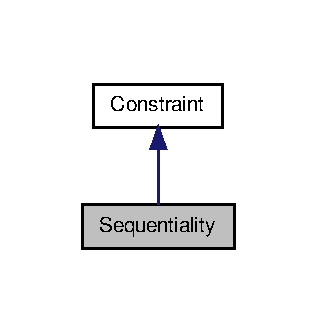
\includegraphics[width=152pt]{classSequentiality__inherit__graph}
\end{center}
\end{figure}


\-Collaboration diagram for \-Sequentiality\-:
\nopagebreak
\begin{figure}[H]
\begin{center}
\leavevmode
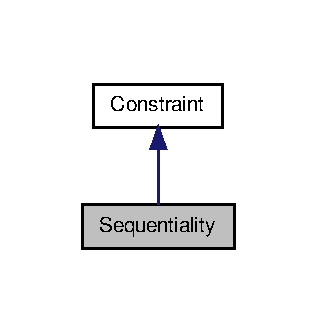
\includegraphics[width=152pt]{classSequentiality__coll__graph}
\end{center}
\end{figure}
\subsection*{\-Public \-Member \-Functions}
\begin{DoxyCompactItemize}
\item 
\hyperlink{classSequentiality_a3d8c4d770b1e057ffe207c47f5db6179}{\-Sequentiality} ()
\item 
virtual \hyperlink{classSequentiality_a7c44312ff2bacacc1716da7594767fbc}{$\sim$\-Sequentiality} ()
\end{DoxyCompactItemize}
\subsection*{\-Protected \-Member \-Functions}
\begin{DoxyCompactItemize}
\item 
void \hyperlink{classSequentiality_a9244bd4d6ff9fe4528658b2adc53fb13}{build\-Matrix\-Ci} ()
\item 
void \hyperlink{classSequentiality_a241b1688f3da2e5accf6ee0799e1c95b}{build\-Matrix\-Cii} ()
\item 
void \hyperlink{classSequentiality_ae115049b18674543e1a7ca2fad039e4b}{build\-Vectord} ()
\end{DoxyCompactItemize}


\subsection{\-Constructor \& \-Destructor \-Documentation}
\hypertarget{classSequentiality_a3d8c4d770b1e057ffe207c47f5db6179}{\index{\-Sequentiality@{\-Sequentiality}!\-Sequentiality@{\-Sequentiality}}
\index{\-Sequentiality@{\-Sequentiality}!Sequentiality@{\-Sequentiality}}
\subsubsection[{\-Sequentiality}]{\setlength{\rightskip}{0pt plus 5cm}{\bf \-Sequentiality\-::\-Sequentiality} (
\begin{DoxyParamCaption}
{}
\end{DoxyParamCaption}
)}}\label{classSequentiality_a3d8c4d770b1e057ffe207c47f5db6179}
\hypertarget{classSequentiality_a7c44312ff2bacacc1716da7594767fbc}{\index{\-Sequentiality@{\-Sequentiality}!$\sim$\-Sequentiality@{$\sim$\-Sequentiality}}
\index{$\sim$\-Sequentiality@{$\sim$\-Sequentiality}!Sequentiality@{\-Sequentiality}}
\subsubsection[{$\sim$\-Sequentiality}]{\setlength{\rightskip}{0pt plus 5cm}{\bf \-Sequentiality\-::$\sim$\-Sequentiality} (
\begin{DoxyParamCaption}
{}
\end{DoxyParamCaption}
)\hspace{0.3cm}{\ttfamily  \mbox{[}virtual\mbox{]}}}}\label{classSequentiality_a7c44312ff2bacacc1716da7594767fbc}


\subsection{\-Member \-Function \-Documentation}
\hypertarget{classSequentiality_a9244bd4d6ff9fe4528658b2adc53fb13}{\index{\-Sequentiality@{\-Sequentiality}!build\-Matrix\-Ci@{build\-Matrix\-Ci}}
\index{build\-Matrix\-Ci@{build\-Matrix\-Ci}!Sequentiality@{\-Sequentiality}}
\subsubsection[{build\-Matrix\-Ci}]{\setlength{\rightskip}{0pt plus 5cm}void {\bf \-Sequentiality\-::build\-Matrix\-Ci} (
\begin{DoxyParamCaption}
{}
\end{DoxyParamCaption}
)\hspace{0.3cm}{\ttfamily  \mbox{[}protected, virtual\mbox{]}}}}\label{classSequentiality_a9244bd4d6ff9fe4528658b2adc53fb13}


\-Reimplemented from \hyperlink{classConstraint_acc08adc7b34825792cb0127a0d699269}{\-Constraint}.

\hypertarget{classSequentiality_a241b1688f3da2e5accf6ee0799e1c95b}{\index{\-Sequentiality@{\-Sequentiality}!build\-Matrix\-Cii@{build\-Matrix\-Cii}}
\index{build\-Matrix\-Cii@{build\-Matrix\-Cii}!Sequentiality@{\-Sequentiality}}
\subsubsection[{build\-Matrix\-Cii}]{\setlength{\rightskip}{0pt plus 5cm}void {\bf \-Sequentiality\-::build\-Matrix\-Cii} (
\begin{DoxyParamCaption}
{}
\end{DoxyParamCaption}
)\hspace{0.3cm}{\ttfamily  \mbox{[}protected, virtual\mbox{]}}}}\label{classSequentiality_a241b1688f3da2e5accf6ee0799e1c95b}


\-Reimplemented from \hyperlink{classConstraint_aef7c4d1071c06f34fbc5c0f06105418f}{\-Constraint}.

\hypertarget{classSequentiality_ae115049b18674543e1a7ca2fad039e4b}{\index{\-Sequentiality@{\-Sequentiality}!build\-Vectord@{build\-Vectord}}
\index{build\-Vectord@{build\-Vectord}!Sequentiality@{\-Sequentiality}}
\subsubsection[{build\-Vectord}]{\setlength{\rightskip}{0pt plus 5cm}void {\bf \-Sequentiality\-::build\-Vectord} (
\begin{DoxyParamCaption}
{}
\end{DoxyParamCaption}
)\hspace{0.3cm}{\ttfamily  \mbox{[}protected, virtual\mbox{]}}}}\label{classSequentiality_ae115049b18674543e1a7ca2fad039e4b}


\-Reimplemented from \hyperlink{classConstraint_a07453509c3f0f95034db965c9e699810}{\-Constraint}.



\-The documentation for this class was generated from the following files\-:\begin{DoxyCompactItemize}
\item 
ocra-\/wbi-\/plugins/ocra-\/icub-\/clients/walking-\/client/include/walking-\/client/constraints/\hyperlink{Sequentiality_8h}{\-Sequentiality.\-h}\item 
ocra-\/wbi-\/plugins/ocra-\/icub-\/clients/walking-\/client/src/\hyperlink{Sequentiality_8cpp}{\-Sequentiality.\-cpp}\end{DoxyCompactItemize}

\hypertarget{structShapeConstraintsStruct_1_1sequentialityStruct}{\section{\-Shape\-Constraints\-Struct\-:\-:sequentiality\-Struct \-Struct \-Reference}
\label{structShapeConstraintsStruct_1_1sequentialityStruct}\index{\-Shape\-Constraints\-Struct\-::sequentiality\-Struct@{\-Shape\-Constraints\-Struct\-::sequentiality\-Struct}}
}


{\ttfamily \#include $<$constraints\-Structs.\-h$>$}

\subsection*{\-Public \-Attributes}
\begin{DoxyCompactItemize}
\item 
\-Eigen\-::\-Matrix\-Xd \hyperlink{structShapeConstraintsStruct_1_1sequentialityStruct_acbb064e5a1baab8b79ffd6c367f31054}{\-C}
\item 
\-Eigen\-::\-Vector\-Xd \hyperlink{structShapeConstraintsStruct_1_1sequentialityStruct_a029a0d4aa9db75b508f9149a262ed28d}{d}
\item 
\-Eigen\-::\-Matrix\-Xd \hyperlink{structShapeConstraintsStruct_1_1sequentialityStruct_a9b9ba6ba7272ef35f2588d852ed967f3}{\-Cbar}
\item 
\-Eigen\-::\-Vector\-Xd \hyperlink{structShapeConstraintsStruct_1_1sequentialityStruct_a68d3aa9f05279aa1ba92e60205a68677}{d\-Bar}
\item 
\-Eigen\-::\-Vector\-Xd \hyperlink{structShapeConstraintsStruct_1_1sequentialityStruct_aa5a0454f0be11f06111cce4ab94db891}{f\-History}
\end{DoxyCompactItemize}


\subsection{\-Member \-Data \-Documentation}
\hypertarget{structShapeConstraintsStruct_1_1sequentialityStruct_acbb064e5a1baab8b79ffd6c367f31054}{\index{\-Shape\-Constraints\-Struct\-::sequentiality\-Struct@{\-Shape\-Constraints\-Struct\-::sequentiality\-Struct}!\-C@{\-C}}
\index{\-C@{\-C}!ShapeConstraintsStruct::sequentialityStruct@{\-Shape\-Constraints\-Struct\-::sequentiality\-Struct}}
\subsubsection[{\-C}]{\setlength{\rightskip}{0pt plus 5cm}\-Eigen\-::\-Matrix\-Xd {\bf \-Shape\-Constraints\-Struct\-::sequentiality\-Struct\-::\-C}}}\label{structShapeConstraintsStruct_1_1sequentialityStruct_acbb064e5a1baab8b79ffd6c367f31054}
\hypertarget{structShapeConstraintsStruct_1_1sequentialityStruct_a9b9ba6ba7272ef35f2588d852ed967f3}{\index{\-Shape\-Constraints\-Struct\-::sequentiality\-Struct@{\-Shape\-Constraints\-Struct\-::sequentiality\-Struct}!\-Cbar@{\-Cbar}}
\index{\-Cbar@{\-Cbar}!ShapeConstraintsStruct::sequentialityStruct@{\-Shape\-Constraints\-Struct\-::sequentiality\-Struct}}
\subsubsection[{\-Cbar}]{\setlength{\rightskip}{0pt plus 5cm}\-Eigen\-::\-Matrix\-Xd {\bf \-Shape\-Constraints\-Struct\-::sequentiality\-Struct\-::\-Cbar}}}\label{structShapeConstraintsStruct_1_1sequentialityStruct_a9b9ba6ba7272ef35f2588d852ed967f3}
\hypertarget{structShapeConstraintsStruct_1_1sequentialityStruct_a029a0d4aa9db75b508f9149a262ed28d}{\index{\-Shape\-Constraints\-Struct\-::sequentiality\-Struct@{\-Shape\-Constraints\-Struct\-::sequentiality\-Struct}!d@{d}}
\index{d@{d}!ShapeConstraintsStruct::sequentialityStruct@{\-Shape\-Constraints\-Struct\-::sequentiality\-Struct}}
\subsubsection[{d}]{\setlength{\rightskip}{0pt plus 5cm}\-Eigen\-::\-Vector\-Xd {\bf \-Shape\-Constraints\-Struct\-::sequentiality\-Struct\-::d}}}\label{structShapeConstraintsStruct_1_1sequentialityStruct_a029a0d4aa9db75b508f9149a262ed28d}
\hypertarget{structShapeConstraintsStruct_1_1sequentialityStruct_a68d3aa9f05279aa1ba92e60205a68677}{\index{\-Shape\-Constraints\-Struct\-::sequentiality\-Struct@{\-Shape\-Constraints\-Struct\-::sequentiality\-Struct}!d\-Bar@{d\-Bar}}
\index{d\-Bar@{d\-Bar}!ShapeConstraintsStruct::sequentialityStruct@{\-Shape\-Constraints\-Struct\-::sequentiality\-Struct}}
\subsubsection[{d\-Bar}]{\setlength{\rightskip}{0pt plus 5cm}\-Eigen\-::\-Vector\-Xd {\bf \-Shape\-Constraints\-Struct\-::sequentiality\-Struct\-::d\-Bar}}}\label{structShapeConstraintsStruct_1_1sequentialityStruct_a68d3aa9f05279aa1ba92e60205a68677}
\hypertarget{structShapeConstraintsStruct_1_1sequentialityStruct_aa5a0454f0be11f06111cce4ab94db891}{\index{\-Shape\-Constraints\-Struct\-::sequentiality\-Struct@{\-Shape\-Constraints\-Struct\-::sequentiality\-Struct}!f\-History@{f\-History}}
\index{f\-History@{f\-History}!ShapeConstraintsStruct::sequentialityStruct@{\-Shape\-Constraints\-Struct\-::sequentiality\-Struct}}
\subsubsection[{f\-History}]{\setlength{\rightskip}{0pt plus 5cm}\-Eigen\-::\-Vector\-Xd {\bf \-Shape\-Constraints\-Struct\-::sequentiality\-Struct\-::f\-History}}}\label{structShapeConstraintsStruct_1_1sequentialityStruct_aa5a0454f0be11f06111cce4ab94db891}


\-The documentation for this struct was generated from the following file\-:\begin{DoxyCompactItemize}
\item 
ocra-\/wbi-\/plugins/ocra-\/icub-\/clients/walking-\/client/include/walking-\/client/\hyperlink{constraintsStructs_8h}{constraints\-Structs.\-h}\end{DoxyCompactItemize}

\hypertarget{classShapeConstraints}{\section{\-Shape\-Constraints \-Class \-Reference}
\label{classShapeConstraints}\index{\-Shape\-Constraints@{\-Shape\-Constraints}}
}


{\ttfamily \#include $<$\-Shape\-Constraints.\-h$>$}



\-Inheritance diagram for \-Shape\-Constraints\-:
\nopagebreak
\begin{figure}[H]
\begin{center}
\leavevmode
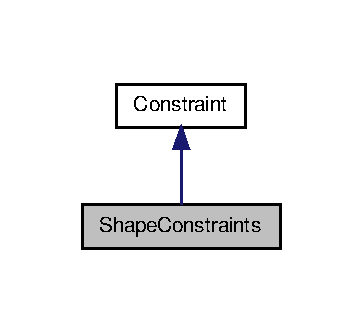
\includegraphics[width=174pt]{classShapeConstraints__inherit__graph}
\end{center}
\end{figure}


\-Collaboration diagram for \-Shape\-Constraints\-:
\nopagebreak
\begin{figure}[H]
\begin{center}
\leavevmode
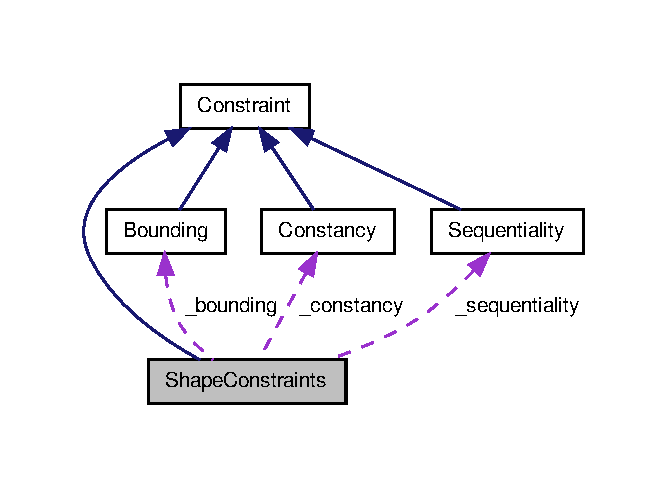
\includegraphics[width=320pt]{classShapeConstraints__coll__graph}
\end{center}
\end{figure}
\subsection*{\-Public \-Member \-Functions}
\begin{DoxyCompactItemize}
\item 
\hyperlink{classShapeConstraints_a64f2900bc242720b52f6546e44858e33}{\-Shape\-Constraints} ()
\item 
virtual \hyperlink{classShapeConstraints_a4da7b352ebe70cdfb8a6bcecbe6986ec}{$\sim$\-Shape\-Constraints} ()
\item 
void \hyperlink{classShapeConstraints_a5106b5a5d1b55e1751423f2af1102c4e}{build\-Matrix\-Ci} ()
\item 
void \hyperlink{classShapeConstraints_a22fcfce709900f384603a759729bdbcd}{build\-Matrix\-Cii} ()
\item 
void \hyperlink{classShapeConstraints_ad7fa37ff0da8688ec2f51add0731a232}{build\-Vectord} ()
\end{DoxyCompactItemize}
\subsection*{\-Protected \-Attributes}
\begin{DoxyCompactItemize}
\item 
\hyperlink{classBounding}{\-Bounding} \hyperlink{classShapeConstraints_aec4139d7b2b7af78543227873fcc9b6c}{\-\_\-bounding}
\item 
\hyperlink{classConstancy}{\-Constancy} \hyperlink{classShapeConstraints_a1682a6b89b7c6c058ccb183b689862a3}{\-\_\-constancy}
\item 
\hyperlink{classSequentiality}{\-Sequentiality} \hyperlink{classShapeConstraints_a0a503cf10835b98ddaa4031a7c63ef42}{\-\_\-sequentiality}
\end{DoxyCompactItemize}


\subsection{\-Constructor \& \-Destructor \-Documentation}
\hypertarget{classShapeConstraints_a64f2900bc242720b52f6546e44858e33}{\index{\-Shape\-Constraints@{\-Shape\-Constraints}!\-Shape\-Constraints@{\-Shape\-Constraints}}
\index{\-Shape\-Constraints@{\-Shape\-Constraints}!ShapeConstraints@{\-Shape\-Constraints}}
\subsubsection[{\-Shape\-Constraints}]{\setlength{\rightskip}{0pt plus 5cm}{\bf \-Shape\-Constraints\-::\-Shape\-Constraints} (
\begin{DoxyParamCaption}
{}
\end{DoxyParamCaption}
)}}\label{classShapeConstraints_a64f2900bc242720b52f6546e44858e33}
\hypertarget{classShapeConstraints_a4da7b352ebe70cdfb8a6bcecbe6986ec}{\index{\-Shape\-Constraints@{\-Shape\-Constraints}!$\sim$\-Shape\-Constraints@{$\sim$\-Shape\-Constraints}}
\index{$\sim$\-Shape\-Constraints@{$\sim$\-Shape\-Constraints}!ShapeConstraints@{\-Shape\-Constraints}}
\subsubsection[{$\sim$\-Shape\-Constraints}]{\setlength{\rightskip}{0pt plus 5cm}{\bf \-Shape\-Constraints\-::$\sim$\-Shape\-Constraints} (
\begin{DoxyParamCaption}
{}
\end{DoxyParamCaption}
)\hspace{0.3cm}{\ttfamily  \mbox{[}virtual\mbox{]}}}}\label{classShapeConstraints_a4da7b352ebe70cdfb8a6bcecbe6986ec}


\subsection{\-Member \-Function \-Documentation}
\hypertarget{classShapeConstraints_a5106b5a5d1b55e1751423f2af1102c4e}{\index{\-Shape\-Constraints@{\-Shape\-Constraints}!build\-Matrix\-Ci@{build\-Matrix\-Ci}}
\index{build\-Matrix\-Ci@{build\-Matrix\-Ci}!ShapeConstraints@{\-Shape\-Constraints}}
\subsubsection[{build\-Matrix\-Ci}]{\setlength{\rightskip}{0pt plus 5cm}void {\bf \-Shape\-Constraints\-::build\-Matrix\-Ci} (
\begin{DoxyParamCaption}
{}
\end{DoxyParamCaption}
)\hspace{0.3cm}{\ttfamily  \mbox{[}virtual\mbox{]}}}}\label{classShapeConstraints_a5106b5a5d1b55e1751423f2af1102c4e}


\-Reimplemented from \hyperlink{classConstraint_acc08adc7b34825792cb0127a0d699269}{\-Constraint}.

\hypertarget{classShapeConstraints_a22fcfce709900f384603a759729bdbcd}{\index{\-Shape\-Constraints@{\-Shape\-Constraints}!build\-Matrix\-Cii@{build\-Matrix\-Cii}}
\index{build\-Matrix\-Cii@{build\-Matrix\-Cii}!ShapeConstraints@{\-Shape\-Constraints}}
\subsubsection[{build\-Matrix\-Cii}]{\setlength{\rightskip}{0pt plus 5cm}void {\bf \-Shape\-Constraints\-::build\-Matrix\-Cii} (
\begin{DoxyParamCaption}
{}
\end{DoxyParamCaption}
)\hspace{0.3cm}{\ttfamily  \mbox{[}virtual\mbox{]}}}}\label{classShapeConstraints_a22fcfce709900f384603a759729bdbcd}


\-Reimplemented from \hyperlink{classConstraint_aef7c4d1071c06f34fbc5c0f06105418f}{\-Constraint}.

\hypertarget{classShapeConstraints_ad7fa37ff0da8688ec2f51add0731a232}{\index{\-Shape\-Constraints@{\-Shape\-Constraints}!build\-Vectord@{build\-Vectord}}
\index{build\-Vectord@{build\-Vectord}!ShapeConstraints@{\-Shape\-Constraints}}
\subsubsection[{build\-Vectord}]{\setlength{\rightskip}{0pt plus 5cm}void {\bf \-Shape\-Constraints\-::build\-Vectord} (
\begin{DoxyParamCaption}
{}
\end{DoxyParamCaption}
)\hspace{0.3cm}{\ttfamily  \mbox{[}virtual\mbox{]}}}}\label{classShapeConstraints_ad7fa37ff0da8688ec2f51add0731a232}


\-Reimplemented from \hyperlink{classConstraint_a07453509c3f0f95034db965c9e699810}{\-Constraint}.



\subsection{\-Member \-Data \-Documentation}
\hypertarget{classShapeConstraints_aec4139d7b2b7af78543227873fcc9b6c}{\index{\-Shape\-Constraints@{\-Shape\-Constraints}!\-\_\-bounding@{\-\_\-bounding}}
\index{\-\_\-bounding@{\-\_\-bounding}!ShapeConstraints@{\-Shape\-Constraints}}
\subsubsection[{\-\_\-bounding}]{\setlength{\rightskip}{0pt plus 5cm}{\bf \-Bounding} {\bf \-Shape\-Constraints\-::\-\_\-bounding}\hspace{0.3cm}{\ttfamily  \mbox{[}protected\mbox{]}}}}\label{classShapeConstraints_aec4139d7b2b7af78543227873fcc9b6c}
\hypertarget{classShapeConstraints_a1682a6b89b7c6c058ccb183b689862a3}{\index{\-Shape\-Constraints@{\-Shape\-Constraints}!\-\_\-constancy@{\-\_\-constancy}}
\index{\-\_\-constancy@{\-\_\-constancy}!ShapeConstraints@{\-Shape\-Constraints}}
\subsubsection[{\-\_\-constancy}]{\setlength{\rightskip}{0pt plus 5cm}{\bf \-Constancy} {\bf \-Shape\-Constraints\-::\-\_\-constancy}\hspace{0.3cm}{\ttfamily  \mbox{[}protected\mbox{]}}}}\label{classShapeConstraints_a1682a6b89b7c6c058ccb183b689862a3}
\hypertarget{classShapeConstraints_a0a503cf10835b98ddaa4031a7c63ef42}{\index{\-Shape\-Constraints@{\-Shape\-Constraints}!\-\_\-sequentiality@{\-\_\-sequentiality}}
\index{\-\_\-sequentiality@{\-\_\-sequentiality}!ShapeConstraints@{\-Shape\-Constraints}}
\subsubsection[{\-\_\-sequentiality}]{\setlength{\rightskip}{0pt plus 5cm}{\bf \-Sequentiality} {\bf \-Shape\-Constraints\-::\-\_\-sequentiality}\hspace{0.3cm}{\ttfamily  \mbox{[}protected\mbox{]}}}}\label{classShapeConstraints_a0a503cf10835b98ddaa4031a7c63ef42}


\-The documentation for this class was generated from the following files\-:\begin{DoxyCompactItemize}
\item 
ocra-\/wbi-\/plugins/ocra-\/icub-\/clients/walking-\/client/include/walking-\/client/constraints/\hyperlink{ShapeConstraints_8h}{\-Shape\-Constraints.\-h}\item 
ocra-\/wbi-\/plugins/ocra-\/icub-\/clients/walking-\/client/src/\hyperlink{ShapeConstraints_8cpp}{\-Shape\-Constraints.\-cpp}\end{DoxyCompactItemize}

\hypertarget{structShapeConstraintsStruct}{\section{\-Shape\-Constraints\-Struct \-Struct \-Reference}
\label{structShapeConstraintsStruct}\index{\-Shape\-Constraints\-Struct@{\-Shape\-Constraints\-Struct}}
}


{\ttfamily \#include $<$constraints\-Structs.\-h$>$}



\-Collaboration diagram for \-Shape\-Constraints\-Struct\-:\nopagebreak
\begin{figure}[H]
\begin{center}
\leavevmode
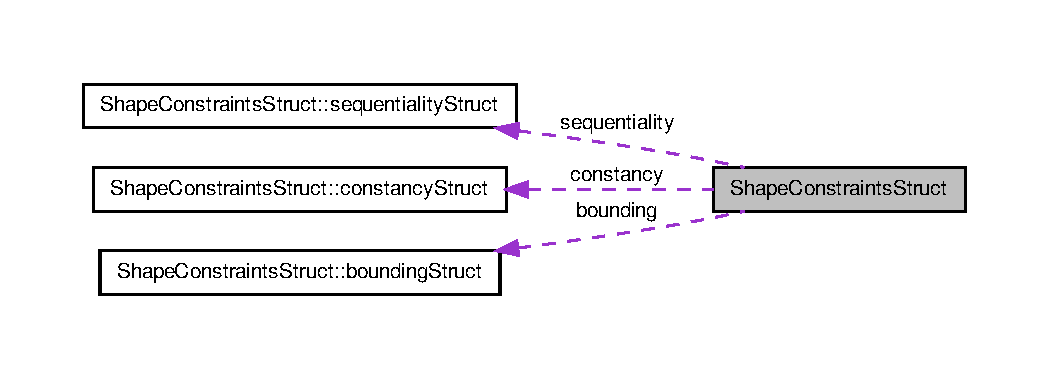
\includegraphics[width=350pt]{structShapeConstraintsStruct__coll__graph}
\end{center}
\end{figure}
\subsection*{\-Classes}
\begin{DoxyCompactItemize}
\item 
struct \hyperlink{structShapeConstraintsStruct_1_1boundingStruct}{bounding\-Struct}
\item 
struct \hyperlink{structShapeConstraintsStruct_1_1constancyStruct}{constancy\-Struct}
\item 
struct \hyperlink{structShapeConstraintsStruct_1_1sequentialityStruct}{sequentiality\-Struct}
\end{DoxyCompactItemize}
\subsection*{\-Public \-Attributes}
\begin{DoxyCompactItemize}
\item 
\-Eigen\-::\-Matrix\-Xd \hyperlink{structShapeConstraintsStruct_ad3e432f9654bd72f28a2dbc146f39aa8}{\-Cbar}
\item 
\-Eigen\-::\-Vector\-Xd \hyperlink{structShapeConstraintsStruct_a8fe2cb4e246df55160e577e690fd1147}{dbar}
\item 
\-Eigen\-::\-Vector\-Xd \hyperlink{structShapeConstraintsStruct_a019f2dc8e024954a9413e0a5c5be9864}{f\-History}
\item 
\hyperlink{structShapeConstraintsStruct_1_1boundingStruct}{bounding\-Struct} \hyperlink{structShapeConstraintsStruct_a54e87c1a5d3df7ca724c4c8437a74ac8}{bounding}
\item 
\hyperlink{structShapeConstraintsStruct_1_1constancyStruct}{constancy\-Struct} \hyperlink{structShapeConstraintsStruct_ab0dfcbbac3869f0464e81facc50a0950}{constancy}
\item 
\hyperlink{structShapeConstraintsStruct_1_1sequentialityStruct}{sequentiality\-Struct} \hyperlink{structShapeConstraintsStruct_ab21948647937089aa8f72ddb8d1536b2}{sequentiality}
\end{DoxyCompactItemize}


\subsection{\-Member \-Data \-Documentation}
\hypertarget{structShapeConstraintsStruct_a54e87c1a5d3df7ca724c4c8437a74ac8}{\index{\-Shape\-Constraints\-Struct@{\-Shape\-Constraints\-Struct}!bounding@{bounding}}
\index{bounding@{bounding}!ShapeConstraintsStruct@{\-Shape\-Constraints\-Struct}}
\subsubsection[{bounding}]{\setlength{\rightskip}{0pt plus 5cm}{\bf bounding\-Struct} {\bf \-Shape\-Constraints\-Struct\-::bounding}}}\label{structShapeConstraintsStruct_a54e87c1a5d3df7ca724c4c8437a74ac8}
\hypertarget{structShapeConstraintsStruct_ad3e432f9654bd72f28a2dbc146f39aa8}{\index{\-Shape\-Constraints\-Struct@{\-Shape\-Constraints\-Struct}!\-Cbar@{\-Cbar}}
\index{\-Cbar@{\-Cbar}!ShapeConstraintsStruct@{\-Shape\-Constraints\-Struct}}
\subsubsection[{\-Cbar}]{\setlength{\rightskip}{0pt plus 5cm}\-Eigen\-::\-Matrix\-Xd {\bf \-Shape\-Constraints\-Struct\-::\-Cbar}}}\label{structShapeConstraintsStruct_ad3e432f9654bd72f28a2dbc146f39aa8}
\hypertarget{structShapeConstraintsStruct_ab0dfcbbac3869f0464e81facc50a0950}{\index{\-Shape\-Constraints\-Struct@{\-Shape\-Constraints\-Struct}!constancy@{constancy}}
\index{constancy@{constancy}!ShapeConstraintsStruct@{\-Shape\-Constraints\-Struct}}
\subsubsection[{constancy}]{\setlength{\rightskip}{0pt plus 5cm}{\bf constancy\-Struct} {\bf \-Shape\-Constraints\-Struct\-::constancy}}}\label{structShapeConstraintsStruct_ab0dfcbbac3869f0464e81facc50a0950}
\hypertarget{structShapeConstraintsStruct_a8fe2cb4e246df55160e577e690fd1147}{\index{\-Shape\-Constraints\-Struct@{\-Shape\-Constraints\-Struct}!dbar@{dbar}}
\index{dbar@{dbar}!ShapeConstraintsStruct@{\-Shape\-Constraints\-Struct}}
\subsubsection[{dbar}]{\setlength{\rightskip}{0pt plus 5cm}\-Eigen\-::\-Vector\-Xd {\bf \-Shape\-Constraints\-Struct\-::dbar}}}\label{structShapeConstraintsStruct_a8fe2cb4e246df55160e577e690fd1147}
\hypertarget{structShapeConstraintsStruct_a019f2dc8e024954a9413e0a5c5be9864}{\index{\-Shape\-Constraints\-Struct@{\-Shape\-Constraints\-Struct}!f\-History@{f\-History}}
\index{f\-History@{f\-History}!ShapeConstraintsStruct@{\-Shape\-Constraints\-Struct}}
\subsubsection[{f\-History}]{\setlength{\rightskip}{0pt plus 5cm}\-Eigen\-::\-Vector\-Xd {\bf \-Shape\-Constraints\-Struct\-::f\-History}}}\label{structShapeConstraintsStruct_a019f2dc8e024954a9413e0a5c5be9864}
\hypertarget{structShapeConstraintsStruct_ab21948647937089aa8f72ddb8d1536b2}{\index{\-Shape\-Constraints\-Struct@{\-Shape\-Constraints\-Struct}!sequentiality@{sequentiality}}
\index{sequentiality@{sequentiality}!ShapeConstraintsStruct@{\-Shape\-Constraints\-Struct}}
\subsubsection[{sequentiality}]{\setlength{\rightskip}{0pt plus 5cm}{\bf sequentiality\-Struct} {\bf \-Shape\-Constraints\-Struct\-::sequentiality}}}\label{structShapeConstraintsStruct_ab21948647937089aa8f72ddb8d1536b2}


\-The documentation for this struct was generated from the following file\-:\begin{DoxyCompactItemize}
\item 
ocra-\/wbi-\/plugins/ocra-\/icub-\/clients/walking-\/client/include/walking-\/client/\hyperlink{constraintsStructs_8h}{constraints\-Structs.\-h}\end{DoxyCompactItemize}

\hypertarget{structsingleStepTestParams}{\section{single\-Step\-Test\-Params \-Struct \-Reference}
\label{structsingleStepTestParams}\index{single\-Step\-Test\-Params@{single\-Step\-Test\-Params}}
}


{\ttfamily \#include $<$utils.\-h$>$}

\subsection*{\-Public \-Attributes}
\begin{DoxyCompactItemize}
\item 
double \hyperlink{structsingleStepTestParams_a64dfd6827254af3491d5ef777a365106}{total\-Duration}
\item 
double \hyperlink{structsingleStepTestParams_a48f06adc433c0802b26a393afa66624e}{offset}
\item 
double \hyperlink{structsingleStepTestParams_a4e63c961cc10a9191f634ea6f7d9d34c}{\-S\-Sduration}
\item 
double \hyperlink{structsingleStepTestParams_ac57481df42dfcc5b6414bba37a6872e7}{rise\-Time}
\item 
double \hyperlink{structsingleStepTestParams_a17bf92e96d709f6cead23bcdcda88d17}{step\-Length}
\item 
double \hyperlink{structsingleStepTestParams_a1b6267edaee10af0a7162065d0ba7a20}{step\-Height}
\end{DoxyCompactItemize}


\subsection{\-Member \-Data \-Documentation}
\hypertarget{structsingleStepTestParams_a48f06adc433c0802b26a393afa66624e}{\index{single\-Step\-Test\-Params@{single\-Step\-Test\-Params}!offset@{offset}}
\index{offset@{offset}!singleStepTestParams@{single\-Step\-Test\-Params}}
\subsubsection[{offset}]{\setlength{\rightskip}{0pt plus 5cm}double {\bf single\-Step\-Test\-Params\-::offset}}}\label{structsingleStepTestParams_a48f06adc433c0802b26a393afa66624e}
\hypertarget{structsingleStepTestParams_ac57481df42dfcc5b6414bba37a6872e7}{\index{single\-Step\-Test\-Params@{single\-Step\-Test\-Params}!rise\-Time@{rise\-Time}}
\index{rise\-Time@{rise\-Time}!singleStepTestParams@{single\-Step\-Test\-Params}}
\subsubsection[{rise\-Time}]{\setlength{\rightskip}{0pt plus 5cm}double {\bf single\-Step\-Test\-Params\-::rise\-Time}}}\label{structsingleStepTestParams_ac57481df42dfcc5b6414bba37a6872e7}
\hypertarget{structsingleStepTestParams_a4e63c961cc10a9191f634ea6f7d9d34c}{\index{single\-Step\-Test\-Params@{single\-Step\-Test\-Params}!\-S\-Sduration@{\-S\-Sduration}}
\index{\-S\-Sduration@{\-S\-Sduration}!singleStepTestParams@{single\-Step\-Test\-Params}}
\subsubsection[{\-S\-Sduration}]{\setlength{\rightskip}{0pt plus 5cm}double {\bf single\-Step\-Test\-Params\-::\-S\-Sduration}}}\label{structsingleStepTestParams_a4e63c961cc10a9191f634ea6f7d9d34c}
\hypertarget{structsingleStepTestParams_a1b6267edaee10af0a7162065d0ba7a20}{\index{single\-Step\-Test\-Params@{single\-Step\-Test\-Params}!step\-Height@{step\-Height}}
\index{step\-Height@{step\-Height}!singleStepTestParams@{single\-Step\-Test\-Params}}
\subsubsection[{step\-Height}]{\setlength{\rightskip}{0pt plus 5cm}double {\bf single\-Step\-Test\-Params\-::step\-Height}}}\label{structsingleStepTestParams_a1b6267edaee10af0a7162065d0ba7a20}
\hypertarget{structsingleStepTestParams_a17bf92e96d709f6cead23bcdcda88d17}{\index{single\-Step\-Test\-Params@{single\-Step\-Test\-Params}!step\-Length@{step\-Length}}
\index{step\-Length@{step\-Length}!singleStepTestParams@{single\-Step\-Test\-Params}}
\subsubsection[{step\-Length}]{\setlength{\rightskip}{0pt plus 5cm}double {\bf single\-Step\-Test\-Params\-::step\-Length}}}\label{structsingleStepTestParams_a17bf92e96d709f6cead23bcdcda88d17}
\hypertarget{structsingleStepTestParams_a64dfd6827254af3491d5ef777a365106}{\index{single\-Step\-Test\-Params@{single\-Step\-Test\-Params}!total\-Duration@{total\-Duration}}
\index{total\-Duration@{total\-Duration}!singleStepTestParams@{single\-Step\-Test\-Params}}
\subsubsection[{total\-Duration}]{\setlength{\rightskip}{0pt plus 5cm}double {\bf single\-Step\-Test\-Params\-::total\-Duration}}}\label{structsingleStepTestParams_a64dfd6827254af3491d5ef777a365106}


\-The documentation for this struct was generated from the following file\-:\begin{DoxyCompactItemize}
\item 
ocra-\/wbi-\/plugins/ocra-\/icub-\/clients/walking-\/client/include/walking-\/client/\hyperlink{utils_8h}{utils.\-h}\end{DoxyCompactItemize}

\hypertarget{classSingleSupport}{\section{\-Single\-Support \-Class \-Reference}
\label{classSingleSupport}\index{\-Single\-Support@{\-Single\-Support}}
}


{\ttfamily \#include $<$\-Single\-Support.\-h$>$}



\-Inheritance diagram for \-Single\-Support\-:\nopagebreak
\begin{figure}[H]
\begin{center}
\leavevmode
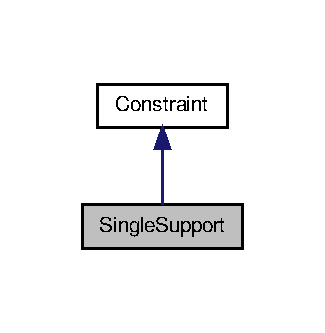
\includegraphics[width=156pt]{classSingleSupport__inherit__graph}
\end{center}
\end{figure}


\-Collaboration diagram for \-Single\-Support\-:\nopagebreak
\begin{figure}[H]
\begin{center}
\leavevmode
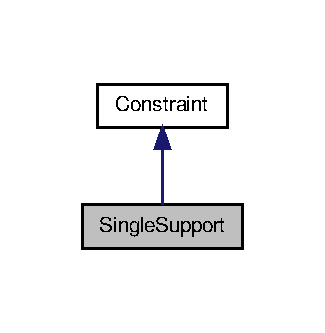
\includegraphics[width=156pt]{classSingleSupport__coll__graph}
\end{center}
\end{figure}
\subsection*{\-Public \-Member \-Functions}
\begin{DoxyCompactItemize}
\item 
\hyperlink{classSingleSupport_af952e77f8d2139224fc0af9b73a6a0d1}{\-Single\-Support} ()
\item 
virtual \hyperlink{classSingleSupport_a56ad004d201bf57cb3472477857b5b38}{$\sim$\-Single\-Support} ()
\end{DoxyCompactItemize}
\subsection*{\-Protected \-Member \-Functions}
\begin{DoxyCompactItemize}
\item 
virtual void \hyperlink{classSingleSupport_a78e5b7c89b828d718560cec73c0f6218}{build\-Matrix\-Ci} ()
\item 
virtual void \hyperlink{classSingleSupport_a746b653c7fbbe989032dadbcfdae3193}{build\-Matrix\-Cii} ()
\item 
virtual void \hyperlink{classSingleSupport_a43caf4b390371ce015cec54d5e78759d}{build\-Vectord} ()
\end{DoxyCompactItemize}
\subsection*{\-Private \-Attributes}
\begin{DoxyCompactItemize}
\item 
\-Eigen\-::\-Vector2d \hyperlink{classSingleSupport_a5b26007c52ad9b2ed45c6ca4f1aef345}{\-\_\-\-S}
\end{DoxyCompactItemize}


\subsection{\-Constructor \& \-Destructor \-Documentation}
\hypertarget{classSingleSupport_af952e77f8d2139224fc0af9b73a6a0d1}{\index{\-Single\-Support@{\-Single\-Support}!\-Single\-Support@{\-Single\-Support}}
\index{\-Single\-Support@{\-Single\-Support}!SingleSupport@{\-Single\-Support}}
\subsubsection[{\-Single\-Support}]{\setlength{\rightskip}{0pt plus 5cm}{\bf \-Single\-Support\-::\-Single\-Support} (
\begin{DoxyParamCaption}
{}
\end{DoxyParamCaption}
)}}\label{classSingleSupport_af952e77f8d2139224fc0af9b73a6a0d1}
\hypertarget{classSingleSupport_a56ad004d201bf57cb3472477857b5b38}{\index{\-Single\-Support@{\-Single\-Support}!$\sim$\-Single\-Support@{$\sim$\-Single\-Support}}
\index{$\sim$\-Single\-Support@{$\sim$\-Single\-Support}!SingleSupport@{\-Single\-Support}}
\subsubsection[{$\sim$\-Single\-Support}]{\setlength{\rightskip}{0pt plus 5cm}{\bf \-Single\-Support\-::$\sim$\-Single\-Support} (
\begin{DoxyParamCaption}
{}
\end{DoxyParamCaption}
)\hspace{0.3cm}{\ttfamily  \mbox{[}virtual\mbox{]}}}}\label{classSingleSupport_a56ad004d201bf57cb3472477857b5b38}


\subsection{\-Member \-Function \-Documentation}
\hypertarget{classSingleSupport_a78e5b7c89b828d718560cec73c0f6218}{\index{\-Single\-Support@{\-Single\-Support}!build\-Matrix\-Ci@{build\-Matrix\-Ci}}
\index{build\-Matrix\-Ci@{build\-Matrix\-Ci}!SingleSupport@{\-Single\-Support}}
\subsubsection[{build\-Matrix\-Ci}]{\setlength{\rightskip}{0pt plus 5cm}void {\bf \-Single\-Support\-::build\-Matrix\-Ci} (
\begin{DoxyParamCaption}
{}
\end{DoxyParamCaption}
)\hspace{0.3cm}{\ttfamily  \mbox{[}protected, virtual\mbox{]}}}}\label{classSingleSupport_a78e5b7c89b828d718560cec73c0f6218}


\-Reimplemented from \hyperlink{classConstraint_acc08adc7b34825792cb0127a0d699269}{\-Constraint}.

\hypertarget{classSingleSupport_a746b653c7fbbe989032dadbcfdae3193}{\index{\-Single\-Support@{\-Single\-Support}!build\-Matrix\-Cii@{build\-Matrix\-Cii}}
\index{build\-Matrix\-Cii@{build\-Matrix\-Cii}!SingleSupport@{\-Single\-Support}}
\subsubsection[{build\-Matrix\-Cii}]{\setlength{\rightskip}{0pt plus 5cm}void {\bf \-Single\-Support\-::build\-Matrix\-Cii} (
\begin{DoxyParamCaption}
{}
\end{DoxyParamCaption}
)\hspace{0.3cm}{\ttfamily  \mbox{[}protected, virtual\mbox{]}}}}\label{classSingleSupport_a746b653c7fbbe989032dadbcfdae3193}


\-Reimplemented from \hyperlink{classConstraint_aef7c4d1071c06f34fbc5c0f06105418f}{\-Constraint}.

\hypertarget{classSingleSupport_a43caf4b390371ce015cec54d5e78759d}{\index{\-Single\-Support@{\-Single\-Support}!build\-Vectord@{build\-Vectord}}
\index{build\-Vectord@{build\-Vectord}!SingleSupport@{\-Single\-Support}}
\subsubsection[{build\-Vectord}]{\setlength{\rightskip}{0pt plus 5cm}void {\bf \-Single\-Support\-::build\-Vectord} (
\begin{DoxyParamCaption}
{}
\end{DoxyParamCaption}
)\hspace{0.3cm}{\ttfamily  \mbox{[}protected, virtual\mbox{]}}}}\label{classSingleSupport_a43caf4b390371ce015cec54d5e78759d}


\-Reimplemented from \hyperlink{classConstraint_a07453509c3f0f95034db965c9e699810}{\-Constraint}.



\subsection{\-Member \-Data \-Documentation}
\hypertarget{classSingleSupport_a5b26007c52ad9b2ed45c6ca4f1aef345}{\index{\-Single\-Support@{\-Single\-Support}!\-\_\-\-S@{\-\_\-\-S}}
\index{\-\_\-\-S@{\-\_\-\-S}!SingleSupport@{\-Single\-Support}}
\subsubsection[{\-\_\-\-S}]{\setlength{\rightskip}{0pt plus 5cm}\-Eigen\-::\-Vector2d {\bf \-Single\-Support\-::\-\_\-\-S}\hspace{0.3cm}{\ttfamily  \mbox{[}private\mbox{]}}}}\label{classSingleSupport_a5b26007c52ad9b2ed45c6ca4f1aef345}


\-The documentation for this class was generated from the following files\-:\begin{DoxyCompactItemize}
\item 
ocra-\/wbi-\/plugins/ocra-\/icub-\/clients/walking-\/client/include/walking-\/client/constraints/\hyperlink{SingleSupport_8h}{\-Single\-Support.\-h}\item 
ocra-\/wbi-\/plugins/ocra-\/icub-\/clients/walking-\/client/src/\hyperlink{SingleSupport_8cpp}{\-Single\-Support.\-cpp}\end{DoxyCompactItemize}

\hypertarget{structAdmissibilityConstraintsStruct_1_1SingleSupport}{\section{\-Admissibility\-Constraints\-Struct\-:\-:\-Single\-Support \-Struct \-Reference}
\label{structAdmissibilityConstraintsStruct_1_1SingleSupport}\index{\-Admissibility\-Constraints\-Struct\-::\-Single\-Support@{\-Admissibility\-Constraints\-Struct\-::\-Single\-Support}}
}


{\ttfamily \#include $<$constraints\-Structs.\-h$>$}

\subsection*{\-Public \-Attributes}
\begin{DoxyCompactItemize}
\item 
\-Eigen\-::\-Matrix\-Xd \hyperlink{structAdmissibilityConstraintsStruct_1_1SingleSupport_abebf0f46c38b599fd621df82309c13f3}{\-C}
\item 
\-Eigen\-::\-Vector\-Xd \hyperlink{structAdmissibilityConstraintsStruct_1_1SingleSupport_aa0a40e7e0a4f8031dc2bf8e9a2da3344}{d}
\item 
\-Eigen\-::\-Matrix\-Xd \hyperlink{structAdmissibilityConstraintsStruct_1_1SingleSupport_a9443a6065e6f1cd7d54b896269d9da1a}{\-Cbar}
\item 
\-Eigen\-::\-Vector\-Xd \hyperlink{structAdmissibilityConstraintsStruct_1_1SingleSupport_adce7d8739e27981f9b6a61e35c261bef}{d\-Bar}
\item 
\-Eigen\-::\-Vector\-Xd \hyperlink{structAdmissibilityConstraintsStruct_1_1SingleSupport_aff9e7430c1d0bb3b5442bda53bb9c842}{\-S}
\item 
\-Eigen\-::\-Vector\-Xd \hyperlink{structAdmissibilityConstraintsStruct_1_1SingleSupport_ad907835e70c7e9c335435b11e733f34d}{f\-History}
\end{DoxyCompactItemize}


\subsection{\-Member \-Data \-Documentation}
\hypertarget{structAdmissibilityConstraintsStruct_1_1SingleSupport_abebf0f46c38b599fd621df82309c13f3}{\index{\-Admissibility\-Constraints\-Struct\-::\-Single\-Support@{\-Admissibility\-Constraints\-Struct\-::\-Single\-Support}!\-C@{\-C}}
\index{\-C@{\-C}!AdmissibilityConstraintsStruct::SingleSupport@{\-Admissibility\-Constraints\-Struct\-::\-Single\-Support}}
\subsubsection[{\-C}]{\setlength{\rightskip}{0pt plus 5cm}\-Eigen\-::\-Matrix\-Xd {\bf \-Admissibility\-Constraints\-Struct\-::\-Single\-Support\-::\-C}}}\label{structAdmissibilityConstraintsStruct_1_1SingleSupport_abebf0f46c38b599fd621df82309c13f3}
\hypertarget{structAdmissibilityConstraintsStruct_1_1SingleSupport_a9443a6065e6f1cd7d54b896269d9da1a}{\index{\-Admissibility\-Constraints\-Struct\-::\-Single\-Support@{\-Admissibility\-Constraints\-Struct\-::\-Single\-Support}!\-Cbar@{\-Cbar}}
\index{\-Cbar@{\-Cbar}!AdmissibilityConstraintsStruct::SingleSupport@{\-Admissibility\-Constraints\-Struct\-::\-Single\-Support}}
\subsubsection[{\-Cbar}]{\setlength{\rightskip}{0pt plus 5cm}\-Eigen\-::\-Matrix\-Xd {\bf \-Admissibility\-Constraints\-Struct\-::\-Single\-Support\-::\-Cbar}}}\label{structAdmissibilityConstraintsStruct_1_1SingleSupport_a9443a6065e6f1cd7d54b896269d9da1a}
\hypertarget{structAdmissibilityConstraintsStruct_1_1SingleSupport_aa0a40e7e0a4f8031dc2bf8e9a2da3344}{\index{\-Admissibility\-Constraints\-Struct\-::\-Single\-Support@{\-Admissibility\-Constraints\-Struct\-::\-Single\-Support}!d@{d}}
\index{d@{d}!AdmissibilityConstraintsStruct::SingleSupport@{\-Admissibility\-Constraints\-Struct\-::\-Single\-Support}}
\subsubsection[{d}]{\setlength{\rightskip}{0pt plus 5cm}\-Eigen\-::\-Vector\-Xd {\bf \-Admissibility\-Constraints\-Struct\-::\-Single\-Support\-::d}}}\label{structAdmissibilityConstraintsStruct_1_1SingleSupport_aa0a40e7e0a4f8031dc2bf8e9a2da3344}
\hypertarget{structAdmissibilityConstraintsStruct_1_1SingleSupport_adce7d8739e27981f9b6a61e35c261bef}{\index{\-Admissibility\-Constraints\-Struct\-::\-Single\-Support@{\-Admissibility\-Constraints\-Struct\-::\-Single\-Support}!d\-Bar@{d\-Bar}}
\index{d\-Bar@{d\-Bar}!AdmissibilityConstraintsStruct::SingleSupport@{\-Admissibility\-Constraints\-Struct\-::\-Single\-Support}}
\subsubsection[{d\-Bar}]{\setlength{\rightskip}{0pt plus 5cm}\-Eigen\-::\-Vector\-Xd {\bf \-Admissibility\-Constraints\-Struct\-::\-Single\-Support\-::d\-Bar}}}\label{structAdmissibilityConstraintsStruct_1_1SingleSupport_adce7d8739e27981f9b6a61e35c261bef}
\hypertarget{structAdmissibilityConstraintsStruct_1_1SingleSupport_ad907835e70c7e9c335435b11e733f34d}{\index{\-Admissibility\-Constraints\-Struct\-::\-Single\-Support@{\-Admissibility\-Constraints\-Struct\-::\-Single\-Support}!f\-History@{f\-History}}
\index{f\-History@{f\-History}!AdmissibilityConstraintsStruct::SingleSupport@{\-Admissibility\-Constraints\-Struct\-::\-Single\-Support}}
\subsubsection[{f\-History}]{\setlength{\rightskip}{0pt plus 5cm}\-Eigen\-::\-Vector\-Xd {\bf \-Admissibility\-Constraints\-Struct\-::\-Single\-Support\-::f\-History}}}\label{structAdmissibilityConstraintsStruct_1_1SingleSupport_ad907835e70c7e9c335435b11e733f34d}
\hypertarget{structAdmissibilityConstraintsStruct_1_1SingleSupport_aff9e7430c1d0bb3b5442bda53bb9c842}{\index{\-Admissibility\-Constraints\-Struct\-::\-Single\-Support@{\-Admissibility\-Constraints\-Struct\-::\-Single\-Support}!\-S@{\-S}}
\index{\-S@{\-S}!AdmissibilityConstraintsStruct::SingleSupport@{\-Admissibility\-Constraints\-Struct\-::\-Single\-Support}}
\subsubsection[{\-S}]{\setlength{\rightskip}{0pt plus 5cm}\-Eigen\-::\-Vector\-Xd {\bf \-Admissibility\-Constraints\-Struct\-::\-Single\-Support\-::\-S}}}\label{structAdmissibilityConstraintsStruct_1_1SingleSupport_aff9e7430c1d0bb3b5442bda53bb9c842}


\-The documentation for this struct was generated from the following file\-:\begin{DoxyCompactItemize}
\item 
ocra-\/wbi-\/plugins/ocra-\/icub-\/clients/walking-\/client/include/walking-\/client/\hyperlink{constraintsStructs_8h}{constraints\-Structs.\-h}\end{DoxyCompactItemize}

\hypertarget{classSittingDemoClient}{\section{\-Sitting\-Demo\-Client \-Class \-Reference}
\label{classSittingDemoClient}\index{\-Sitting\-Demo\-Client@{\-Sitting\-Demo\-Client}}
}


{\ttfamily \#include $<$\-Sitting\-Demo\-Client.\-h$>$}

\subsection*{\-Public \-Member \-Functions}
\begin{DoxyCompactItemize}
\item 
\hyperlink{classSittingDemoClient_aedcb6c4ad7b4fa19f1b188e700c0a079}{\-Sitting\-Demo\-Client} (std\-::shared\-\_\-ptr$<$ ocra\-::\-Model $>$ model\-Ptr, const int loop\-Period)
\item 
virtual \hyperlink{classSittingDemoClient_a0fb7ded5e44b2b60d7f89c22386154b7}{$\sim$\-Sitting\-Demo\-Client} ()
\end{DoxyCompactItemize}
\subsection*{\-Protected \-Member \-Functions}
\begin{DoxyCompactItemize}
\item 
virtual bool \hyperlink{classSittingDemoClient_aff04405d690f2ae8abbd05ea4b55b64d}{initialize} ()
\item 
virtual void \hyperlink{classSittingDemoClient_a18d30d70a9b17e8f64f87f5cb01b746e}{release} ()
\item 
virtual void \hyperlink{classSittingDemoClient_ad08cf3328c8a4f22a1677b5ad67de645}{loop} ()
\end{DoxyCompactItemize}
\subsection*{\-Private \-Attributes}
\begin{DoxyCompactItemize}
\item 
ocra\-\_\-recipes\-::\-Trajectory\-Thread\-::\-Ptr \hyperlink{classSittingDemoClient_a1d5616269e9a673022542bb86f380bfd}{root\-Traj\-Thread}
\end{DoxyCompactItemize}


\subsection{\-Constructor \& \-Destructor \-Documentation}
\hypertarget{classSittingDemoClient_aedcb6c4ad7b4fa19f1b188e700c0a079}{\index{\-Sitting\-Demo\-Client@{\-Sitting\-Demo\-Client}!\-Sitting\-Demo\-Client@{\-Sitting\-Demo\-Client}}
\index{\-Sitting\-Demo\-Client@{\-Sitting\-Demo\-Client}!SittingDemoClient@{\-Sitting\-Demo\-Client}}
\subsubsection[{\-Sitting\-Demo\-Client}]{\setlength{\rightskip}{0pt plus 5cm}{\bf \-Sitting\-Demo\-Client\-::\-Sitting\-Demo\-Client} (
\begin{DoxyParamCaption}
\item[{std\-::shared\-\_\-ptr$<$ ocra\-::\-Model $>$}]{model\-Ptr, }
\item[{const int}]{loop\-Period}
\end{DoxyParamCaption}
)}}\label{classSittingDemoClient_aedcb6c4ad7b4fa19f1b188e700c0a079}
\hypertarget{classSittingDemoClient_a0fb7ded5e44b2b60d7f89c22386154b7}{\index{\-Sitting\-Demo\-Client@{\-Sitting\-Demo\-Client}!$\sim$\-Sitting\-Demo\-Client@{$\sim$\-Sitting\-Demo\-Client}}
\index{$\sim$\-Sitting\-Demo\-Client@{$\sim$\-Sitting\-Demo\-Client}!SittingDemoClient@{\-Sitting\-Demo\-Client}}
\subsubsection[{$\sim$\-Sitting\-Demo\-Client}]{\setlength{\rightskip}{0pt plus 5cm}{\bf \-Sitting\-Demo\-Client\-::$\sim$\-Sitting\-Demo\-Client} (
\begin{DoxyParamCaption}
{}
\end{DoxyParamCaption}
)\hspace{0.3cm}{\ttfamily  \mbox{[}virtual\mbox{]}}}}\label{classSittingDemoClient_a0fb7ded5e44b2b60d7f89c22386154b7}


\subsection{\-Member \-Function \-Documentation}
\hypertarget{classSittingDemoClient_aff04405d690f2ae8abbd05ea4b55b64d}{\index{\-Sitting\-Demo\-Client@{\-Sitting\-Demo\-Client}!initialize@{initialize}}
\index{initialize@{initialize}!SittingDemoClient@{\-Sitting\-Demo\-Client}}
\subsubsection[{initialize}]{\setlength{\rightskip}{0pt plus 5cm}bool {\bf \-Sitting\-Demo\-Client\-::initialize} (
\begin{DoxyParamCaption}
{}
\end{DoxyParamCaption}
)\hspace{0.3cm}{\ttfamily  \mbox{[}protected, virtual\mbox{]}}}}\label{classSittingDemoClient_aff04405d690f2ae8abbd05ea4b55b64d}
\hypertarget{classSittingDemoClient_ad08cf3328c8a4f22a1677b5ad67de645}{\index{\-Sitting\-Demo\-Client@{\-Sitting\-Demo\-Client}!loop@{loop}}
\index{loop@{loop}!SittingDemoClient@{\-Sitting\-Demo\-Client}}
\subsubsection[{loop}]{\setlength{\rightskip}{0pt plus 5cm}void {\bf \-Sitting\-Demo\-Client\-::loop} (
\begin{DoxyParamCaption}
{}
\end{DoxyParamCaption}
)\hspace{0.3cm}{\ttfamily  \mbox{[}protected, virtual\mbox{]}}}}\label{classSittingDemoClient_ad08cf3328c8a4f22a1677b5ad67de645}
\hypertarget{classSittingDemoClient_a18d30d70a9b17e8f64f87f5cb01b746e}{\index{\-Sitting\-Demo\-Client@{\-Sitting\-Demo\-Client}!release@{release}}
\index{release@{release}!SittingDemoClient@{\-Sitting\-Demo\-Client}}
\subsubsection[{release}]{\setlength{\rightskip}{0pt plus 5cm}void {\bf \-Sitting\-Demo\-Client\-::release} (
\begin{DoxyParamCaption}
{}
\end{DoxyParamCaption}
)\hspace{0.3cm}{\ttfamily  \mbox{[}protected, virtual\mbox{]}}}}\label{classSittingDemoClient_a18d30d70a9b17e8f64f87f5cb01b746e}


\subsection{\-Member \-Data \-Documentation}
\hypertarget{classSittingDemoClient_a1d5616269e9a673022542bb86f380bfd}{\index{\-Sitting\-Demo\-Client@{\-Sitting\-Demo\-Client}!root\-Traj\-Thread@{root\-Traj\-Thread}}
\index{root\-Traj\-Thread@{root\-Traj\-Thread}!SittingDemoClient@{\-Sitting\-Demo\-Client}}
\subsubsection[{root\-Traj\-Thread}]{\setlength{\rightskip}{0pt plus 5cm}ocra\-\_\-recipes\-::\-Trajectory\-Thread\-::\-Ptr {\bf \-Sitting\-Demo\-Client\-::root\-Traj\-Thread}\hspace{0.3cm}{\ttfamily  \mbox{[}private\mbox{]}}}}\label{classSittingDemoClient_a1d5616269e9a673022542bb86f380bfd}


\-The documentation for this class was generated from the following files\-:\begin{DoxyCompactItemize}
\item 
ocra-\/wbi-\/plugins/ocra-\/icub-\/clients/sitting-\/demo/include/sitting-\/demo/\hyperlink{SittingDemoClient_8h}{\-Sitting\-Demo\-Client.\-h}\item 
ocra-\/wbi-\/plugins/ocra-\/icub-\/clients/sitting-\/demo/src/\hyperlink{SittingDemoClient_8cpp}{\-Sitting\-Demo\-Client.\-cpp}\end{DoxyCompactItemize}

\hypertarget{structAdmissibilityConstraintsStruct_1_1SSandDSAlternation}{\section{\-Admissibility\-Constraints\-Struct\-:\-:\-S\-Sand\-D\-S\-Alternation \-Struct \-Reference}
\label{structAdmissibilityConstraintsStruct_1_1SSandDSAlternation}\index{\-Admissibility\-Constraints\-Struct\-::\-S\-Sand\-D\-S\-Alternation@{\-Admissibility\-Constraints\-Struct\-::\-S\-Sand\-D\-S\-Alternation}}
}


{\ttfamily \#include $<$constraints\-Structs.\-h$>$}

\subsection*{\-Public \-Attributes}
\begin{DoxyCompactItemize}
\item 
\-Eigen\-::\-Matrix\-Xd \hyperlink{structAdmissibilityConstraintsStruct_1_1SSandDSAlternation_ad8c275715499505ab842c0aa3cf422fe}{\-C1}
\item 
\-Eigen\-::\-Matrix\-Xd \hyperlink{structAdmissibilityConstraintsStruct_1_1SSandDSAlternation_a5c169268d67d6a949dea763b6f71c4c5}{\-C2}
\item 
\-Eigen\-::\-Vector\-Xd \hyperlink{structAdmissibilityConstraintsStruct_1_1SSandDSAlternation_ab40c36a6b9d326f612d7380493716bbc}{d}
\item 
\-Eigen\-::\-Matrix\-Xd \hyperlink{structAdmissibilityConstraintsStruct_1_1SSandDSAlternation_ac6c3cf83c627777487ad717c1cf9b40f}{\-C1bar}
\item 
\-Eigen\-::\-Matrix\-Xd \hyperlink{structAdmissibilityConstraintsStruct_1_1SSandDSAlternation_aa2118aa17c20af2515c770ba9943f52b}{\-C2bar}
\item 
\-Eigen\-::\-Vector\-Xd \hyperlink{structAdmissibilityConstraintsStruct_1_1SSandDSAlternation_a9099e9134eefdb5d540ec8a3eec5acb6}{d\-Bar}
\item 
\-Eigen\-::\-Vector\-Xd \hyperlink{structAdmissibilityConstraintsStruct_1_1SSandDSAlternation_abacb8f39b18c0960834a0ebc1d46ba28}{f\-History}
\end{DoxyCompactItemize}


\subsection{\-Member \-Data \-Documentation}
\hypertarget{structAdmissibilityConstraintsStruct_1_1SSandDSAlternation_ad8c275715499505ab842c0aa3cf422fe}{\index{\-Admissibility\-Constraints\-Struct\-::\-S\-Sand\-D\-S\-Alternation@{\-Admissibility\-Constraints\-Struct\-::\-S\-Sand\-D\-S\-Alternation}!\-C1@{\-C1}}
\index{\-C1@{\-C1}!AdmissibilityConstraintsStruct::SSandDSAlternation@{\-Admissibility\-Constraints\-Struct\-::\-S\-Sand\-D\-S\-Alternation}}
\subsubsection[{\-C1}]{\setlength{\rightskip}{0pt plus 5cm}\-Eigen\-::\-Matrix\-Xd {\bf \-Admissibility\-Constraints\-Struct\-::\-S\-Sand\-D\-S\-Alternation\-::\-C1}}}\label{structAdmissibilityConstraintsStruct_1_1SSandDSAlternation_ad8c275715499505ab842c0aa3cf422fe}
\hypertarget{structAdmissibilityConstraintsStruct_1_1SSandDSAlternation_ac6c3cf83c627777487ad717c1cf9b40f}{\index{\-Admissibility\-Constraints\-Struct\-::\-S\-Sand\-D\-S\-Alternation@{\-Admissibility\-Constraints\-Struct\-::\-S\-Sand\-D\-S\-Alternation}!\-C1bar@{\-C1bar}}
\index{\-C1bar@{\-C1bar}!AdmissibilityConstraintsStruct::SSandDSAlternation@{\-Admissibility\-Constraints\-Struct\-::\-S\-Sand\-D\-S\-Alternation}}
\subsubsection[{\-C1bar}]{\setlength{\rightskip}{0pt plus 5cm}\-Eigen\-::\-Matrix\-Xd {\bf \-Admissibility\-Constraints\-Struct\-::\-S\-Sand\-D\-S\-Alternation\-::\-C1bar}}}\label{structAdmissibilityConstraintsStruct_1_1SSandDSAlternation_ac6c3cf83c627777487ad717c1cf9b40f}
\hypertarget{structAdmissibilityConstraintsStruct_1_1SSandDSAlternation_a5c169268d67d6a949dea763b6f71c4c5}{\index{\-Admissibility\-Constraints\-Struct\-::\-S\-Sand\-D\-S\-Alternation@{\-Admissibility\-Constraints\-Struct\-::\-S\-Sand\-D\-S\-Alternation}!\-C2@{\-C2}}
\index{\-C2@{\-C2}!AdmissibilityConstraintsStruct::SSandDSAlternation@{\-Admissibility\-Constraints\-Struct\-::\-S\-Sand\-D\-S\-Alternation}}
\subsubsection[{\-C2}]{\setlength{\rightskip}{0pt plus 5cm}\-Eigen\-::\-Matrix\-Xd {\bf \-Admissibility\-Constraints\-Struct\-::\-S\-Sand\-D\-S\-Alternation\-::\-C2}}}\label{structAdmissibilityConstraintsStruct_1_1SSandDSAlternation_a5c169268d67d6a949dea763b6f71c4c5}
\hypertarget{structAdmissibilityConstraintsStruct_1_1SSandDSAlternation_aa2118aa17c20af2515c770ba9943f52b}{\index{\-Admissibility\-Constraints\-Struct\-::\-S\-Sand\-D\-S\-Alternation@{\-Admissibility\-Constraints\-Struct\-::\-S\-Sand\-D\-S\-Alternation}!\-C2bar@{\-C2bar}}
\index{\-C2bar@{\-C2bar}!AdmissibilityConstraintsStruct::SSandDSAlternation@{\-Admissibility\-Constraints\-Struct\-::\-S\-Sand\-D\-S\-Alternation}}
\subsubsection[{\-C2bar}]{\setlength{\rightskip}{0pt plus 5cm}\-Eigen\-::\-Matrix\-Xd {\bf \-Admissibility\-Constraints\-Struct\-::\-S\-Sand\-D\-S\-Alternation\-::\-C2bar}}}\label{structAdmissibilityConstraintsStruct_1_1SSandDSAlternation_aa2118aa17c20af2515c770ba9943f52b}
\hypertarget{structAdmissibilityConstraintsStruct_1_1SSandDSAlternation_ab40c36a6b9d326f612d7380493716bbc}{\index{\-Admissibility\-Constraints\-Struct\-::\-S\-Sand\-D\-S\-Alternation@{\-Admissibility\-Constraints\-Struct\-::\-S\-Sand\-D\-S\-Alternation}!d@{d}}
\index{d@{d}!AdmissibilityConstraintsStruct::SSandDSAlternation@{\-Admissibility\-Constraints\-Struct\-::\-S\-Sand\-D\-S\-Alternation}}
\subsubsection[{d}]{\setlength{\rightskip}{0pt plus 5cm}\-Eigen\-::\-Vector\-Xd {\bf \-Admissibility\-Constraints\-Struct\-::\-S\-Sand\-D\-S\-Alternation\-::d}}}\label{structAdmissibilityConstraintsStruct_1_1SSandDSAlternation_ab40c36a6b9d326f612d7380493716bbc}
\hypertarget{structAdmissibilityConstraintsStruct_1_1SSandDSAlternation_a9099e9134eefdb5d540ec8a3eec5acb6}{\index{\-Admissibility\-Constraints\-Struct\-::\-S\-Sand\-D\-S\-Alternation@{\-Admissibility\-Constraints\-Struct\-::\-S\-Sand\-D\-S\-Alternation}!d\-Bar@{d\-Bar}}
\index{d\-Bar@{d\-Bar}!AdmissibilityConstraintsStruct::SSandDSAlternation@{\-Admissibility\-Constraints\-Struct\-::\-S\-Sand\-D\-S\-Alternation}}
\subsubsection[{d\-Bar}]{\setlength{\rightskip}{0pt plus 5cm}\-Eigen\-::\-Vector\-Xd {\bf \-Admissibility\-Constraints\-Struct\-::\-S\-Sand\-D\-S\-Alternation\-::d\-Bar}}}\label{structAdmissibilityConstraintsStruct_1_1SSandDSAlternation_a9099e9134eefdb5d540ec8a3eec5acb6}
\hypertarget{structAdmissibilityConstraintsStruct_1_1SSandDSAlternation_abacb8f39b18c0960834a0ebc1d46ba28}{\index{\-Admissibility\-Constraints\-Struct\-::\-S\-Sand\-D\-S\-Alternation@{\-Admissibility\-Constraints\-Struct\-::\-S\-Sand\-D\-S\-Alternation}!f\-History@{f\-History}}
\index{f\-History@{f\-History}!AdmissibilityConstraintsStruct::SSandDSAlternation@{\-Admissibility\-Constraints\-Struct\-::\-S\-Sand\-D\-S\-Alternation}}
\subsubsection[{f\-History}]{\setlength{\rightskip}{0pt plus 5cm}\-Eigen\-::\-Vector\-Xd {\bf \-Admissibility\-Constraints\-Struct\-::\-S\-Sand\-D\-S\-Alternation\-::f\-History}}}\label{structAdmissibilityConstraintsStruct_1_1SSandDSAlternation_abacb8f39b18c0960834a0ebc1d46ba28}


\-The documentation for this struct was generated from the following file\-:\begin{DoxyCompactItemize}
\item 
ocra-\/wbi-\/plugins/ocra-\/icub-\/clients/walking-\/client/include/walking-\/client/\hyperlink{constraintsStructs_8h}{constraints\-Structs.\-h}\end{DoxyCompactItemize}

\hypertarget{classSSDSAlternation}{\section{\-S\-S\-D\-S\-Alternation \-Class \-Reference}
\label{classSSDSAlternation}\index{\-S\-S\-D\-S\-Alternation@{\-S\-S\-D\-S\-Alternation}}
}


{\ttfamily \#include $<$\-S\-S\-D\-S\-Alternation.\-h$>$}



\-Inheritance diagram for \-S\-S\-D\-S\-Alternation\-:
\nopagebreak
\begin{figure}[H]
\begin{center}
\leavevmode
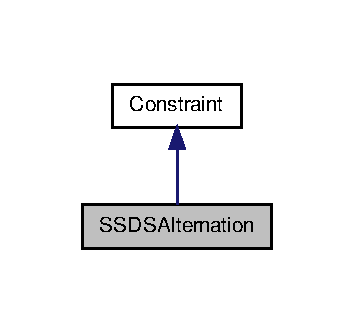
\includegraphics[width=170pt]{classSSDSAlternation__inherit__graph}
\end{center}
\end{figure}


\-Collaboration diagram for \-S\-S\-D\-S\-Alternation\-:
\nopagebreak
\begin{figure}[H]
\begin{center}
\leavevmode
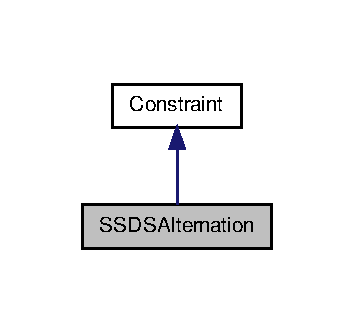
\includegraphics[width=170pt]{classSSDSAlternation__coll__graph}
\end{center}
\end{figure}
\subsection*{\-Public \-Member \-Functions}
\begin{DoxyCompactItemize}
\item 
\hyperlink{classSSDSAlternation_a4f163d6400aac19c61c47d7ce0bdd7fd}{\-S\-S\-D\-S\-Alternation} ()
\item 
virtual \hyperlink{classSSDSAlternation_ac5a0ff4ee8a18bb6ebaaa436a4a901ee}{$\sim$\-S\-S\-D\-S\-Alternation} ()
\end{DoxyCompactItemize}
\subsection*{\-Protected \-Member \-Functions}
\begin{DoxyCompactItemize}
\item 
void \hyperlink{classSSDSAlternation_af4e463bf49d5863366c38de3e3f5e74b}{build\-Matrix\-Ci} ()
\item 
void \hyperlink{classSSDSAlternation_aa527e6b2639391ccd602392e7dceba1e}{build\-Matrix\-Cii} ()
\item 
void \hyperlink{classSSDSAlternation_ac081b561d5553ca392157304662b3b13}{build\-Vectord} ()
\end{DoxyCompactItemize}


\subsection{\-Constructor \& \-Destructor \-Documentation}
\hypertarget{classSSDSAlternation_a4f163d6400aac19c61c47d7ce0bdd7fd}{\index{\-S\-S\-D\-S\-Alternation@{\-S\-S\-D\-S\-Alternation}!\-S\-S\-D\-S\-Alternation@{\-S\-S\-D\-S\-Alternation}}
\index{\-S\-S\-D\-S\-Alternation@{\-S\-S\-D\-S\-Alternation}!SSDSAlternation@{\-S\-S\-D\-S\-Alternation}}
\subsubsection[{\-S\-S\-D\-S\-Alternation}]{\setlength{\rightskip}{0pt plus 5cm}{\bf \-S\-S\-D\-S\-Alternation\-::\-S\-S\-D\-S\-Alternation} (
\begin{DoxyParamCaption}
{}
\end{DoxyParamCaption}
)}}\label{classSSDSAlternation_a4f163d6400aac19c61c47d7ce0bdd7fd}
\hypertarget{classSSDSAlternation_ac5a0ff4ee8a18bb6ebaaa436a4a901ee}{\index{\-S\-S\-D\-S\-Alternation@{\-S\-S\-D\-S\-Alternation}!$\sim$\-S\-S\-D\-S\-Alternation@{$\sim$\-S\-S\-D\-S\-Alternation}}
\index{$\sim$\-S\-S\-D\-S\-Alternation@{$\sim$\-S\-S\-D\-S\-Alternation}!SSDSAlternation@{\-S\-S\-D\-S\-Alternation}}
\subsubsection[{$\sim$\-S\-S\-D\-S\-Alternation}]{\setlength{\rightskip}{0pt plus 5cm}{\bf \-S\-S\-D\-S\-Alternation\-::$\sim$\-S\-S\-D\-S\-Alternation} (
\begin{DoxyParamCaption}
{}
\end{DoxyParamCaption}
)\hspace{0.3cm}{\ttfamily  \mbox{[}virtual\mbox{]}}}}\label{classSSDSAlternation_ac5a0ff4ee8a18bb6ebaaa436a4a901ee}


\subsection{\-Member \-Function \-Documentation}
\hypertarget{classSSDSAlternation_af4e463bf49d5863366c38de3e3f5e74b}{\index{\-S\-S\-D\-S\-Alternation@{\-S\-S\-D\-S\-Alternation}!build\-Matrix\-Ci@{build\-Matrix\-Ci}}
\index{build\-Matrix\-Ci@{build\-Matrix\-Ci}!SSDSAlternation@{\-S\-S\-D\-S\-Alternation}}
\subsubsection[{build\-Matrix\-Ci}]{\setlength{\rightskip}{0pt plus 5cm}void {\bf \-S\-S\-D\-S\-Alternation\-::build\-Matrix\-Ci} (
\begin{DoxyParamCaption}
{}
\end{DoxyParamCaption}
)\hspace{0.3cm}{\ttfamily  \mbox{[}protected, virtual\mbox{]}}}}\label{classSSDSAlternation_af4e463bf49d5863366c38de3e3f5e74b}


\-Reimplemented from \hyperlink{classConstraint_acc08adc7b34825792cb0127a0d699269}{\-Constraint}.

\hypertarget{classSSDSAlternation_aa527e6b2639391ccd602392e7dceba1e}{\index{\-S\-S\-D\-S\-Alternation@{\-S\-S\-D\-S\-Alternation}!build\-Matrix\-Cii@{build\-Matrix\-Cii}}
\index{build\-Matrix\-Cii@{build\-Matrix\-Cii}!SSDSAlternation@{\-S\-S\-D\-S\-Alternation}}
\subsubsection[{build\-Matrix\-Cii}]{\setlength{\rightskip}{0pt plus 5cm}void {\bf \-S\-S\-D\-S\-Alternation\-::build\-Matrix\-Cii} (
\begin{DoxyParamCaption}
{}
\end{DoxyParamCaption}
)\hspace{0.3cm}{\ttfamily  \mbox{[}protected, virtual\mbox{]}}}}\label{classSSDSAlternation_aa527e6b2639391ccd602392e7dceba1e}


\-Reimplemented from \hyperlink{classConstraint_aef7c4d1071c06f34fbc5c0f06105418f}{\-Constraint}.

\hypertarget{classSSDSAlternation_ac081b561d5553ca392157304662b3b13}{\index{\-S\-S\-D\-S\-Alternation@{\-S\-S\-D\-S\-Alternation}!build\-Vectord@{build\-Vectord}}
\index{build\-Vectord@{build\-Vectord}!SSDSAlternation@{\-S\-S\-D\-S\-Alternation}}
\subsubsection[{build\-Vectord}]{\setlength{\rightskip}{0pt plus 5cm}void {\bf \-S\-S\-D\-S\-Alternation\-::build\-Vectord} (
\begin{DoxyParamCaption}
{}
\end{DoxyParamCaption}
)\hspace{0.3cm}{\ttfamily  \mbox{[}protected, virtual\mbox{]}}}}\label{classSSDSAlternation_ac081b561d5553ca392157304662b3b13}


\-Reimplemented from \hyperlink{classConstraint_a07453509c3f0f95034db965c9e699810}{\-Constraint}.



\-The documentation for this class was generated from the following files\-:\begin{DoxyCompactItemize}
\item 
ocra-\/wbi-\/plugins/ocra-\/icub-\/clients/walking-\/client/include/walking-\/client/constraints/\hyperlink{SSDSAlternation_8h}{\-S\-S\-D\-S\-Alternation.\-h}\item 
ocra-\/wbi-\/plugins/ocra-\/icub-\/clients/walking-\/client/src/\hyperlink{SSDSAlternation_8cpp}{\-S\-S\-D\-S\-Alternation.\-cpp}\end{DoxyCompactItemize}

\hypertarget{classStandingDemoClient}{\section{\-Standing\-Demo\-Client \-Class \-Reference}
\label{classStandingDemoClient}\index{\-Standing\-Demo\-Client@{\-Standing\-Demo\-Client}}
}


{\ttfamily \#include $<$\-Standing\-Demo\-Client.\-h$>$}

\subsection*{\-Public \-Member \-Functions}
\begin{DoxyCompactItemize}
\item 
\hyperlink{classStandingDemoClient_a7fc81439cf274825e81f243fab4ee94a}{\-Standing\-Demo\-Client} (std\-::shared\-\_\-ptr$<$ ocra\-::\-Model $>$ model\-Ptr, const int loop\-Period)
\item 
virtual \hyperlink{classStandingDemoClient_a36afdcb86f9e304c53f9903d6b286dd7}{$\sim$\-Standing\-Demo\-Client} ()
\item 
bool \hyperlink{classStandingDemoClient_a9cca697399c183d9e2e5fe5b45dbc815}{configure} (yarp\-::os\-::\-Resource\-Finder \&rf)
\end{DoxyCompactItemize}
\subsection*{\-Protected \-Member \-Functions}
\begin{DoxyCompactItemize}
\item 
virtual bool \hyperlink{classStandingDemoClient_a0219c4ae161543b6ea797f27f345593c}{initialize} ()
\item 
virtual void \hyperlink{classStandingDemoClient_abdc4f3642b1ab31ba16375e55a7a68f4}{release} ()
\item 
virtual void \hyperlink{classStandingDemoClient_a294411fb3f128a6a8f5011ea6330af6e}{loop} ()
\item 
virtual void \hyperlink{classStandingDemoClient_ae1f321428f6b67b2f8bf7e1e7a1cd3d4}{print\-Help} ()
\end{DoxyCompactItemize}
\subsection*{\-Private \-Member \-Functions}
\begin{DoxyCompactItemize}
\item 
void \hyperlink{classStandingDemoClient_a6a16f7c8b66d49c6fc63f75ce8eaaf0b}{deactivate\-Leg\-Contacts} ()
\end{DoxyCompactItemize}
\subsection*{\-Private \-Attributes}
\begin{DoxyCompactItemize}
\item 
double \hyperlink{classStandingDemoClient_a638e427aef4c4dc6fa38081ab5f9f405}{max\-Vel}
\item 
double \hyperlink{classStandingDemoClient_abc06fc0343cbca7a3faac4dbb1eaa842}{max\-Acc}
\item 
bool \hyperlink{classStandingDemoClient_a47132d5336d2e3b02085d2f153db6385}{use\-Min\-Jerk}
\item 
ocra\-\_\-recipes\-::\-Trajectory\-Thread\-::\-Ptr \hyperlink{classStandingDemoClient_a223aa634ceba696716779461ec1d3f63}{com\-Traj\-Thread}
\item 
ocra\-\_\-recipes\-::\-Trajectory\-Thread\-::\-Ptr \hyperlink{classStandingDemoClient_a4f84e52d8be94fb7fae7a6c0ad8e8adb}{root\-Traj\-Thread}
\item 
ocra\-\_\-recipes\-::\-Task\-Connection\-::\-Ptr \hyperlink{classStandingDemoClient_ad5dfa4632f03e75095c810b6ff2301b4}{left\-Leg\-Contact\-Task}
\item 
ocra\-\_\-recipes\-::\-Task\-Connection\-::\-Ptr \hyperlink{classStandingDemoClient_ad53b834a0927d48917f5b6e830feb0f8}{right\-Leg\-Contact\-Task}
\item 
double \hyperlink{classStandingDemoClient_af05ac205216c20f9780f7e48a9ee4648}{start\-Time}
\item 
double \hyperlink{classStandingDemoClient_a4a13f8bdbc84e3645c7a1ab69012c652}{contact\-Release\-Delay}
\item 
bool \hyperlink{classStandingDemoClient_ac6744005797ac8071776a68b35a7da6d}{contacts\-Released}
\end{DoxyCompactItemize}


\subsection{\-Constructor \& \-Destructor \-Documentation}
\hypertarget{classStandingDemoClient_a7fc81439cf274825e81f243fab4ee94a}{\index{\-Standing\-Demo\-Client@{\-Standing\-Demo\-Client}!\-Standing\-Demo\-Client@{\-Standing\-Demo\-Client}}
\index{\-Standing\-Demo\-Client@{\-Standing\-Demo\-Client}!StandingDemoClient@{\-Standing\-Demo\-Client}}
\subsubsection[{\-Standing\-Demo\-Client}]{\setlength{\rightskip}{0pt plus 5cm}{\bf \-Standing\-Demo\-Client\-::\-Standing\-Demo\-Client} (
\begin{DoxyParamCaption}
\item[{std\-::shared\-\_\-ptr$<$ ocra\-::\-Model $>$}]{model\-Ptr, }
\item[{const int}]{loop\-Period}
\end{DoxyParamCaption}
)}}\label{classStandingDemoClient_a7fc81439cf274825e81f243fab4ee94a}
\hypertarget{classStandingDemoClient_a36afdcb86f9e304c53f9903d6b286dd7}{\index{\-Standing\-Demo\-Client@{\-Standing\-Demo\-Client}!$\sim$\-Standing\-Demo\-Client@{$\sim$\-Standing\-Demo\-Client}}
\index{$\sim$\-Standing\-Demo\-Client@{$\sim$\-Standing\-Demo\-Client}!StandingDemoClient@{\-Standing\-Demo\-Client}}
\subsubsection[{$\sim$\-Standing\-Demo\-Client}]{\setlength{\rightskip}{0pt plus 5cm}{\bf \-Standing\-Demo\-Client\-::$\sim$\-Standing\-Demo\-Client} (
\begin{DoxyParamCaption}
{}
\end{DoxyParamCaption}
)\hspace{0.3cm}{\ttfamily  \mbox{[}virtual\mbox{]}}}}\label{classStandingDemoClient_a36afdcb86f9e304c53f9903d6b286dd7}


\subsection{\-Member \-Function \-Documentation}
\hypertarget{classStandingDemoClient_a9cca697399c183d9e2e5fe5b45dbc815}{\index{\-Standing\-Demo\-Client@{\-Standing\-Demo\-Client}!configure@{configure}}
\index{configure@{configure}!StandingDemoClient@{\-Standing\-Demo\-Client}}
\subsubsection[{configure}]{\setlength{\rightskip}{0pt plus 5cm}bool {\bf \-Standing\-Demo\-Client\-::configure} (
\begin{DoxyParamCaption}
\item[{yarp\-::os\-::\-Resource\-Finder \&}]{rf}
\end{DoxyParamCaption}
)}}\label{classStandingDemoClient_a9cca697399c183d9e2e5fe5b45dbc815}
\hypertarget{classStandingDemoClient_a6a16f7c8b66d49c6fc63f75ce8eaaf0b}{\index{\-Standing\-Demo\-Client@{\-Standing\-Demo\-Client}!deactivate\-Leg\-Contacts@{deactivate\-Leg\-Contacts}}
\index{deactivate\-Leg\-Contacts@{deactivate\-Leg\-Contacts}!StandingDemoClient@{\-Standing\-Demo\-Client}}
\subsubsection[{deactivate\-Leg\-Contacts}]{\setlength{\rightskip}{0pt plus 5cm}void {\bf \-Standing\-Demo\-Client\-::deactivate\-Leg\-Contacts} (
\begin{DoxyParamCaption}
{}
\end{DoxyParamCaption}
)\hspace{0.3cm}{\ttfamily  \mbox{[}private\mbox{]}}}}\label{classStandingDemoClient_a6a16f7c8b66d49c6fc63f75ce8eaaf0b}
\hypertarget{classStandingDemoClient_a0219c4ae161543b6ea797f27f345593c}{\index{\-Standing\-Demo\-Client@{\-Standing\-Demo\-Client}!initialize@{initialize}}
\index{initialize@{initialize}!StandingDemoClient@{\-Standing\-Demo\-Client}}
\subsubsection[{initialize}]{\setlength{\rightskip}{0pt plus 5cm}bool {\bf \-Standing\-Demo\-Client\-::initialize} (
\begin{DoxyParamCaption}
{}
\end{DoxyParamCaption}
)\hspace{0.3cm}{\ttfamily  \mbox{[}protected, virtual\mbox{]}}}}\label{classStandingDemoClient_a0219c4ae161543b6ea797f27f345593c}
\hypertarget{classStandingDemoClient_a294411fb3f128a6a8f5011ea6330af6e}{\index{\-Standing\-Demo\-Client@{\-Standing\-Demo\-Client}!loop@{loop}}
\index{loop@{loop}!StandingDemoClient@{\-Standing\-Demo\-Client}}
\subsubsection[{loop}]{\setlength{\rightskip}{0pt plus 5cm}void {\bf \-Standing\-Demo\-Client\-::loop} (
\begin{DoxyParamCaption}
{}
\end{DoxyParamCaption}
)\hspace{0.3cm}{\ttfamily  \mbox{[}protected, virtual\mbox{]}}}}\label{classStandingDemoClient_a294411fb3f128a6a8f5011ea6330af6e}
\hypertarget{classStandingDemoClient_ae1f321428f6b67b2f8bf7e1e7a1cd3d4}{\index{\-Standing\-Demo\-Client@{\-Standing\-Demo\-Client}!print\-Help@{print\-Help}}
\index{print\-Help@{print\-Help}!StandingDemoClient@{\-Standing\-Demo\-Client}}
\subsubsection[{print\-Help}]{\setlength{\rightskip}{0pt plus 5cm}void {\bf \-Standing\-Demo\-Client\-::print\-Help} (
\begin{DoxyParamCaption}
{}
\end{DoxyParamCaption}
)\hspace{0.3cm}{\ttfamily  \mbox{[}protected, virtual\mbox{]}}}}\label{classStandingDemoClient_ae1f321428f6b67b2f8bf7e1e7a1cd3d4}
\hypertarget{classStandingDemoClient_abdc4f3642b1ab31ba16375e55a7a68f4}{\index{\-Standing\-Demo\-Client@{\-Standing\-Demo\-Client}!release@{release}}
\index{release@{release}!StandingDemoClient@{\-Standing\-Demo\-Client}}
\subsubsection[{release}]{\setlength{\rightskip}{0pt plus 5cm}void {\bf \-Standing\-Demo\-Client\-::release} (
\begin{DoxyParamCaption}
{}
\end{DoxyParamCaption}
)\hspace{0.3cm}{\ttfamily  \mbox{[}protected, virtual\mbox{]}}}}\label{classStandingDemoClient_abdc4f3642b1ab31ba16375e55a7a68f4}


\subsection{\-Member \-Data \-Documentation}
\hypertarget{classStandingDemoClient_a223aa634ceba696716779461ec1d3f63}{\index{\-Standing\-Demo\-Client@{\-Standing\-Demo\-Client}!com\-Traj\-Thread@{com\-Traj\-Thread}}
\index{com\-Traj\-Thread@{com\-Traj\-Thread}!StandingDemoClient@{\-Standing\-Demo\-Client}}
\subsubsection[{com\-Traj\-Thread}]{\setlength{\rightskip}{0pt plus 5cm}ocra\-\_\-recipes\-::\-Trajectory\-Thread\-::\-Ptr {\bf \-Standing\-Demo\-Client\-::com\-Traj\-Thread}\hspace{0.3cm}{\ttfamily  \mbox{[}private\mbox{]}}}}\label{classStandingDemoClient_a223aa634ceba696716779461ec1d3f63}
\hypertarget{classStandingDemoClient_a4a13f8bdbc84e3645c7a1ab69012c652}{\index{\-Standing\-Demo\-Client@{\-Standing\-Demo\-Client}!contact\-Release\-Delay@{contact\-Release\-Delay}}
\index{contact\-Release\-Delay@{contact\-Release\-Delay}!StandingDemoClient@{\-Standing\-Demo\-Client}}
\subsubsection[{contact\-Release\-Delay}]{\setlength{\rightskip}{0pt plus 5cm}double {\bf \-Standing\-Demo\-Client\-::contact\-Release\-Delay}\hspace{0.3cm}{\ttfamily  \mbox{[}private\mbox{]}}}}\label{classStandingDemoClient_a4a13f8bdbc84e3645c7a1ab69012c652}
\hypertarget{classStandingDemoClient_ac6744005797ac8071776a68b35a7da6d}{\index{\-Standing\-Demo\-Client@{\-Standing\-Demo\-Client}!contacts\-Released@{contacts\-Released}}
\index{contacts\-Released@{contacts\-Released}!StandingDemoClient@{\-Standing\-Demo\-Client}}
\subsubsection[{contacts\-Released}]{\setlength{\rightskip}{0pt plus 5cm}bool {\bf \-Standing\-Demo\-Client\-::contacts\-Released}\hspace{0.3cm}{\ttfamily  \mbox{[}private\mbox{]}}}}\label{classStandingDemoClient_ac6744005797ac8071776a68b35a7da6d}
\hypertarget{classStandingDemoClient_ad5dfa4632f03e75095c810b6ff2301b4}{\index{\-Standing\-Demo\-Client@{\-Standing\-Demo\-Client}!left\-Leg\-Contact\-Task@{left\-Leg\-Contact\-Task}}
\index{left\-Leg\-Contact\-Task@{left\-Leg\-Contact\-Task}!StandingDemoClient@{\-Standing\-Demo\-Client}}
\subsubsection[{left\-Leg\-Contact\-Task}]{\setlength{\rightskip}{0pt plus 5cm}ocra\-\_\-recipes\-::\-Task\-Connection\-::\-Ptr {\bf \-Standing\-Demo\-Client\-::left\-Leg\-Contact\-Task}\hspace{0.3cm}{\ttfamily  \mbox{[}private\mbox{]}}}}\label{classStandingDemoClient_ad5dfa4632f03e75095c810b6ff2301b4}
\hypertarget{classStandingDemoClient_abc06fc0343cbca7a3faac4dbb1eaa842}{\index{\-Standing\-Demo\-Client@{\-Standing\-Demo\-Client}!max\-Acc@{max\-Acc}}
\index{max\-Acc@{max\-Acc}!StandingDemoClient@{\-Standing\-Demo\-Client}}
\subsubsection[{max\-Acc}]{\setlength{\rightskip}{0pt plus 5cm}double {\bf \-Standing\-Demo\-Client\-::max\-Acc}\hspace{0.3cm}{\ttfamily  \mbox{[}private\mbox{]}}}}\label{classStandingDemoClient_abc06fc0343cbca7a3faac4dbb1eaa842}
\hypertarget{classStandingDemoClient_a638e427aef4c4dc6fa38081ab5f9f405}{\index{\-Standing\-Demo\-Client@{\-Standing\-Demo\-Client}!max\-Vel@{max\-Vel}}
\index{max\-Vel@{max\-Vel}!StandingDemoClient@{\-Standing\-Demo\-Client}}
\subsubsection[{max\-Vel}]{\setlength{\rightskip}{0pt plus 5cm}double {\bf \-Standing\-Demo\-Client\-::max\-Vel}\hspace{0.3cm}{\ttfamily  \mbox{[}private\mbox{]}}}}\label{classStandingDemoClient_a638e427aef4c4dc6fa38081ab5f9f405}
\hypertarget{classStandingDemoClient_ad53b834a0927d48917f5b6e830feb0f8}{\index{\-Standing\-Demo\-Client@{\-Standing\-Demo\-Client}!right\-Leg\-Contact\-Task@{right\-Leg\-Contact\-Task}}
\index{right\-Leg\-Contact\-Task@{right\-Leg\-Contact\-Task}!StandingDemoClient@{\-Standing\-Demo\-Client}}
\subsubsection[{right\-Leg\-Contact\-Task}]{\setlength{\rightskip}{0pt plus 5cm}ocra\-\_\-recipes\-::\-Task\-Connection\-::\-Ptr {\bf \-Standing\-Demo\-Client\-::right\-Leg\-Contact\-Task}\hspace{0.3cm}{\ttfamily  \mbox{[}private\mbox{]}}}}\label{classStandingDemoClient_ad53b834a0927d48917f5b6e830feb0f8}
\hypertarget{classStandingDemoClient_a4f84e52d8be94fb7fae7a6c0ad8e8adb}{\index{\-Standing\-Demo\-Client@{\-Standing\-Demo\-Client}!root\-Traj\-Thread@{root\-Traj\-Thread}}
\index{root\-Traj\-Thread@{root\-Traj\-Thread}!StandingDemoClient@{\-Standing\-Demo\-Client}}
\subsubsection[{root\-Traj\-Thread}]{\setlength{\rightskip}{0pt plus 5cm}ocra\-\_\-recipes\-::\-Trajectory\-Thread\-::\-Ptr {\bf \-Standing\-Demo\-Client\-::root\-Traj\-Thread}\hspace{0.3cm}{\ttfamily  \mbox{[}private\mbox{]}}}}\label{classStandingDemoClient_a4f84e52d8be94fb7fae7a6c0ad8e8adb}
\hypertarget{classStandingDemoClient_af05ac205216c20f9780f7e48a9ee4648}{\index{\-Standing\-Demo\-Client@{\-Standing\-Demo\-Client}!start\-Time@{start\-Time}}
\index{start\-Time@{start\-Time}!StandingDemoClient@{\-Standing\-Demo\-Client}}
\subsubsection[{start\-Time}]{\setlength{\rightskip}{0pt plus 5cm}double {\bf \-Standing\-Demo\-Client\-::start\-Time}\hspace{0.3cm}{\ttfamily  \mbox{[}private\mbox{]}}}}\label{classStandingDemoClient_af05ac205216c20f9780f7e48a9ee4648}
\hypertarget{classStandingDemoClient_a47132d5336d2e3b02085d2f153db6385}{\index{\-Standing\-Demo\-Client@{\-Standing\-Demo\-Client}!use\-Min\-Jerk@{use\-Min\-Jerk}}
\index{use\-Min\-Jerk@{use\-Min\-Jerk}!StandingDemoClient@{\-Standing\-Demo\-Client}}
\subsubsection[{use\-Min\-Jerk}]{\setlength{\rightskip}{0pt plus 5cm}bool {\bf \-Standing\-Demo\-Client\-::use\-Min\-Jerk}\hspace{0.3cm}{\ttfamily  \mbox{[}private\mbox{]}}}}\label{classStandingDemoClient_a47132d5336d2e3b02085d2f153db6385}


\-The documentation for this class was generated from the following files\-:\begin{DoxyCompactItemize}
\item 
ocra-\/wbi-\/plugins/ocra-\/icub-\/clients/standing-\/demo/include/standing-\/demo/\hyperlink{StandingDemoClient_8h}{\-Standing\-Demo\-Client.\-h}\item 
ocra-\/wbi-\/plugins/ocra-\/icub-\/clients/standing-\/demo/src/\hyperlink{StandingDemoClient_8cpp}{\-Standing\-Demo\-Client.\-cpp}\end{DoxyCompactItemize}

\hypertarget{classStepController}{\section{\-Step\-Controller \-Class \-Reference}
\label{classStepController}\index{\-Step\-Controller@{\-Step\-Controller}}
}


{\ttfamily \#include $<$\-Step\-Controller.\-h$>$}

\subsection*{\-Public \-Member \-Functions}
\begin{DoxyCompactItemize}
\item 
\hyperlink{classStepController_a80b7436dcb5c1d4a3e04f805b8f8f32a}{\-Step\-Controller} (int periodms, ocra\-::\-Model\-::\-Ptr model)
\item 
virtual \hyperlink{classStepController_ae2033c937309c104539b6758346529d5}{$\sim$\-Step\-Controller} ()
\item 
bool \hyperlink{classStepController_a8f061f201c651d920ca02f7daa07adfe}{initialize} ()
\item 
void \hyperlink{classStepController_ada72856c76030cc22ebb18f368f829f1}{deactivate\-Feet\-Contacts} (\hyperlink{utils_8h_a4b6a8e135f90bd56e5a57a60efb42529}{\-F\-O\-O\-T} foot)
\item 
void \hyperlink{classStepController_a6184693a199603c945250a58ceb8d9a2}{activate\-Feet\-Contacts} (\hyperlink{utils_8h_a4b6a8e135f90bd56e5a57a60efb42529}{\-F\-O\-O\-T} foot)
\item 
bool \hyperlink{classStepController_a1bfcb66d504440f0cc7383ad688dad5c}{do\-Step\-With\-Max\-Velocity} (\hyperlink{utils_8h_a4b6a8e135f90bd56e5a57a60efb42529}{\-F\-O\-O\-T} foot, \-Eigen\-::\-Vector3d \hyperlink{classStepController_a588d5b149eb4a6877e89ecff37d0f91d}{target}, double step\-Height)
\item 
\-Eigen\-::\-Vector3d \hyperlink{classStepController_aa168e028dc086859400e1c93c0becdd2}{get\-Left\-Foot\-Position} ()
\item 
\-Eigen\-::\-Vector3d \hyperlink{classStepController_aaa7e389226a30582be8c8a724661a921}{get\-Right\-Foot\-Position} ()
\item 
void \hyperlink{classStepController_a0dcf2ec0d0fdf1fd9d86878fffd4e5ad}{compute\-Mid\-Point} (\hyperlink{utils_8h_a4b6a8e135f90bd56e5a57a60efb42529}{\-F\-O\-O\-T} foot, \-Eigen\-::\-Vector3d \hyperlink{classStepController_a588d5b149eb4a6877e89ecff37d0f91d}{target}, double step\-Height, \-Eigen\-::\-Vector3d \&mid\-Point)
\item 
void \hyperlink{classStepController_a16b1f62737f1287b7f33b216871d1ba8}{do\-Compute\-Mid\-Point} (\-Eigen\-::\-Vector3d current\-Foot\-Position, \-Eigen\-::\-Vector3d \hyperlink{classStepController_a588d5b149eb4a6877e89ecff37d0f91d}{target}, double step\-Height, \-Eigen\-::\-Vector3d \&mid\-Point)
\item 
bool \hyperlink{classStepController_a9e2415755548f47301277feb7a376270}{is\-Trajectory\-Finished} (\hyperlink{utils_8h_a4b6a8e135f90bd56e5a57a60efb42529}{\-F\-O\-O\-T} foot)
\item 
void \hyperlink{classStepController_a48224628b92c088a34d9db4a14f75f1a}{stop} ()
\item 
\-Eigen\-::\-Matrix\-Xd \hyperlink{classStepController_afb77002292921660ef4a44657d6566f1}{get\-Contact2\-D\-Coordinates} ()
\end{DoxyCompactItemize}
\subsection*{\-Private \-Attributes}
\begin{DoxyCompactItemize}
\item 
std\-::vector\*
$<$ ocra\-\_\-recipes\-::\-Task\-Connection\-::\-Ptr $>$ \hyperlink{classStepController_aabeb4837b7b6cf691cb9de57c6ea8800}{\-\_\-contacts\-Collection}
\item 
ocra\-\_\-recipes\-::\-Task\-Connection\-::\-Ptr \hyperlink{classStepController_ad778378c6e6ac12d972cc8c5a986dcf9}{\-\_\-\-Left\-Foot\-Contact\-\_\-\-Back\-Left}
\item 
ocra\-\_\-recipes\-::\-Task\-Connection\-::\-Ptr \hyperlink{classStepController_a74e19501ce4f336bb4c26beebe3d39e2}{\-\_\-\-Left\-Foot\-Contact\-\_\-\-Front\-Left}
\item 
ocra\-\_\-recipes\-::\-Task\-Connection\-::\-Ptr \hyperlink{classStepController_a9c733b7ab0ce610c84158f7d1de60267}{\-\_\-\-Left\-Foot\-Contact\-\_\-\-Back\-Right}
\item 
ocra\-\_\-recipes\-::\-Task\-Connection\-::\-Ptr \hyperlink{classStepController_a1a4e831d573ab9e0f25680da7d065a77}{\-\_\-\-Left\-Foot\-Contact\-\_\-\-Front\-Right}
\item 
ocra\-\_\-recipes\-::\-Task\-Connection\-::\-Ptr \hyperlink{classStepController_a57947ee8824b3cb3ee34e936431588df}{\-\_\-\-Right\-Foot\-Contact\-\_\-\-Back\-Left}
\item 
ocra\-\_\-recipes\-::\-Task\-Connection\-::\-Ptr \hyperlink{classStepController_a0e1c5ce837e4811214a97c42edc66721}{\-\_\-\-Right\-Foot\-Contact\-\_\-\-Front\-Left}
\item 
ocra\-\_\-recipes\-::\-Task\-Connection\-::\-Ptr \hyperlink{classStepController_ac999bb1e7b4b005da35093345c0cb4de}{\-\_\-\-Right\-Foot\-Contact\-\_\-\-Back\-Right}
\item 
ocra\-\_\-recipes\-::\-Task\-Connection\-::\-Ptr \hyperlink{classStepController_a9f06562625b657c280dc688bcad421be}{\-\_\-\-Right\-Foot\-Contact\-\_\-\-Front\-Right}
\item 
std\-::shared\-\_\-ptr\*
$<$ ocra\-\_\-recipes\-::\-Trajectory\-Thread $>$ \hyperlink{classStepController_adc2b0bf2d3c302c54d659d44cb34ba3e}{\-\_\-left\-Foot\-\_\-\-Traj\-Thread}
\item 
std\-::shared\-\_\-ptr\*
$<$ ocra\-\_\-recipes\-::\-Trajectory\-Thread $>$ \hyperlink{classStepController_a37b943ed8733490d028687997944e478}{\-\_\-right\-Foot\-\_\-\-Traj\-Thread}
\item 
\-Eigen\-::\-Vector3d \hyperlink{classStepController_a588d5b149eb4a6877e89ecff37d0f91d}{target}
\item 
\-Eigen\-::\-Vector3d \hyperlink{classStepController_a6bc27bbd20adf3bc0a1b010a14dece95}{\-\_\-left\-Foot\-Position}
\item 
\-Eigen\-::\-Vector3d \hyperlink{classStepController_a064d9f5406f9221e4351617a177c1cef}{\-\_\-right\-Foot\-Position}
\item 
ocra\-::\-Model\-::\-Ptr \hyperlink{classStepController_aa07914c0186c24fd4fc02612d0ee6332}{\-\_\-model}
\item 
int \hyperlink{classStepController_a8b98494b6b9d13b41c6838d127078085}{\-\_\-period}
\end{DoxyCompactItemize}


\subsection{\-Detailed \-Description}
\begin{DoxyNote}{\-Note}

\end{DoxyNote}
\begin{DoxyAuthor}{\-Author}
\-Jorhabib \-Eljaik
\end{DoxyAuthor}
\begin{DoxyWarning}{\-Warning}
\-Work in progress! \-This is still a barebone class in the process of being tested. 
\end{DoxyWarning}


\subsection{\-Constructor \& \-Destructor \-Documentation}
\hypertarget{classStepController_a80b7436dcb5c1d4a3e04f805b8f8f32a}{\index{\-Step\-Controller@{\-Step\-Controller}!\-Step\-Controller@{\-Step\-Controller}}
\index{\-Step\-Controller@{\-Step\-Controller}!StepController@{\-Step\-Controller}}
\subsubsection[{\-Step\-Controller}]{\setlength{\rightskip}{0pt plus 5cm}{\bf \-Step\-Controller\-::\-Step\-Controller} (
\begin{DoxyParamCaption}
\item[{int}]{periodms, }
\item[{ocra\-::\-Model\-::\-Ptr}]{model}
\end{DoxyParamCaption}
)}}\label{classStepController_a80b7436dcb5c1d4a3e04f805b8f8f32a}
\hypertarget{classStepController_ae2033c937309c104539b6758346529d5}{\index{\-Step\-Controller@{\-Step\-Controller}!$\sim$\-Step\-Controller@{$\sim$\-Step\-Controller}}
\index{$\sim$\-Step\-Controller@{$\sim$\-Step\-Controller}!StepController@{\-Step\-Controller}}
\subsubsection[{$\sim$\-Step\-Controller}]{\setlength{\rightskip}{0pt plus 5cm}{\bf \-Step\-Controller\-::$\sim$\-Step\-Controller} (
\begin{DoxyParamCaption}
{}
\end{DoxyParamCaption}
)\hspace{0.3cm}{\ttfamily  \mbox{[}virtual\mbox{]}}}}\label{classStepController_ae2033c937309c104539b6758346529d5}


\subsection{\-Member \-Function \-Documentation}
\hypertarget{classStepController_a6184693a199603c945250a58ceb8d9a2}{\index{\-Step\-Controller@{\-Step\-Controller}!activate\-Feet\-Contacts@{activate\-Feet\-Contacts}}
\index{activate\-Feet\-Contacts@{activate\-Feet\-Contacts}!StepController@{\-Step\-Controller}}
\subsubsection[{activate\-Feet\-Contacts}]{\setlength{\rightskip}{0pt plus 5cm}void {\bf \-Step\-Controller\-::activate\-Feet\-Contacts} (
\begin{DoxyParamCaption}
\item[{{\bf \-F\-O\-O\-T}}]{foot}
\end{DoxyParamCaption}
)}}\label{classStepController_a6184693a199603c945250a58ceb8d9a2}
\-This method asks the ocra-\/icub-\/server to activate one by one the feet \char`\"{}corner\char`\"{} contact tasks for the specified foot.


\begin{DoxyParams}{\-Parameters}
{\em foot} & \-L\-E\-F\-T\-\_\-\-F\-O\-O\-T or \-R\-I\-G\-H\-T\-\_\-\-F\-O\-O\-T. \\
\hline
\end{DoxyParams}
\hypertarget{classStepController_a0dcf2ec0d0fdf1fd9d86878fffd4e5ad}{\index{\-Step\-Controller@{\-Step\-Controller}!compute\-Mid\-Point@{compute\-Mid\-Point}}
\index{compute\-Mid\-Point@{compute\-Mid\-Point}!StepController@{\-Step\-Controller}}
\subsubsection[{compute\-Mid\-Point}]{\setlength{\rightskip}{0pt plus 5cm}void {\bf \-Step\-Controller\-::compute\-Mid\-Point} (
\begin{DoxyParamCaption}
\item[{{\bf \-F\-O\-O\-T}}]{foot, }
\item[{\-Eigen\-::\-Vector3d}]{target, }
\item[{double}]{step\-Height, }
\item[{\-Eigen\-::\-Vector3d \&}]{mid\-Point}
\end{DoxyParamCaption}
)}}\label{classStepController_a0dcf2ec0d0fdf1fd9d86878fffd4e5ad}
\hypertarget{classStepController_ada72856c76030cc22ebb18f368f829f1}{\index{\-Step\-Controller@{\-Step\-Controller}!deactivate\-Feet\-Contacts@{deactivate\-Feet\-Contacts}}
\index{deactivate\-Feet\-Contacts@{deactivate\-Feet\-Contacts}!StepController@{\-Step\-Controller}}
\subsubsection[{deactivate\-Feet\-Contacts}]{\setlength{\rightskip}{0pt plus 5cm}void {\bf \-Step\-Controller\-::deactivate\-Feet\-Contacts} (
\begin{DoxyParamCaption}
\item[{{\bf \-F\-O\-O\-T}}]{foot}
\end{DoxyParamCaption}
)}}\label{classStepController_ada72856c76030cc22ebb18f368f829f1}
\-Remember the right and left feet contact tasks? created in \hyperlink{classStepController_a8f061f201c651d920ca02f7daa07adfe}{initialize()}. \-This method asks the ocra-\/icub-\/server to deactivate one by one the feet \char`\"{}corner\char`\"{} contact tasks for the specified foot.


\begin{DoxyParams}{\-Parameters}
{\em foot} & \-L\-E\-F\-T\-\_\-\-F\-O\-O\-T or \-R\-I\-G\-H\-T\-\_\-\-F\-O\-O\-T. \\
\hline
\end{DoxyParams}
\hypertarget{classStepController_a16b1f62737f1287b7f33b216871d1ba8}{\index{\-Step\-Controller@{\-Step\-Controller}!do\-Compute\-Mid\-Point@{do\-Compute\-Mid\-Point}}
\index{do\-Compute\-Mid\-Point@{do\-Compute\-Mid\-Point}!StepController@{\-Step\-Controller}}
\subsubsection[{do\-Compute\-Mid\-Point}]{\setlength{\rightskip}{0pt plus 5cm}void {\bf \-Step\-Controller\-::do\-Compute\-Mid\-Point} (
\begin{DoxyParamCaption}
\item[{\-Eigen\-::\-Vector3d}]{current\-Foot\-Position, }
\item[{\-Eigen\-::\-Vector3d}]{target, }
\item[{double}]{step\-Height, }
\item[{\-Eigen\-::\-Vector3d \&}]{mid\-Point}
\end{DoxyParamCaption}
)}}\label{classStepController_a16b1f62737f1287b7f33b216871d1ba8}
\hypertarget{classStepController_a1bfcb66d504440f0cc7383ad688dad5c}{\index{\-Step\-Controller@{\-Step\-Controller}!do\-Step\-With\-Max\-Velocity@{do\-Step\-With\-Max\-Velocity}}
\index{do\-Step\-With\-Max\-Velocity@{do\-Step\-With\-Max\-Velocity}!StepController@{\-Step\-Controller}}
\subsubsection[{do\-Step\-With\-Max\-Velocity}]{\setlength{\rightskip}{0pt plus 5cm}bool {\bf \-Step\-Controller\-::do\-Step\-With\-Max\-Velocity} (
\begin{DoxyParamCaption}
\item[{{\bf \-F\-O\-O\-T}}]{foot, }
\item[{\-Eigen\-::\-Vector3d}]{target, }
\item[{double}]{step\-Height}
\end{DoxyParamCaption}
)}}\label{classStepController_a1bfcb66d504440f0cc7383ad688dad5c}
\hypertarget{classStepController_afb77002292921660ef4a44657d6566f1}{\index{\-Step\-Controller@{\-Step\-Controller}!get\-Contact2\-D\-Coordinates@{get\-Contact2\-D\-Coordinates}}
\index{get\-Contact2\-D\-Coordinates@{get\-Contact2\-D\-Coordinates}!StepController@{\-Step\-Controller}}
\subsubsection[{get\-Contact2\-D\-Coordinates}]{\setlength{\rightskip}{0pt plus 5cm}\-Eigen\-::\-Matrix\-Xd {\bf \-Step\-Controller\-::get\-Contact2\-D\-Coordinates} (
\begin{DoxyParamCaption}
{}
\end{DoxyParamCaption}
)}}\label{classStepController_afb77002292921660ef4a44657d6566f1}
\-Returns the 2\-D coordinates of the contacts defined at the task level.

\begin{DoxyReturn}{\-Returns}
\-Matrix of 2\-D coordinates of the contact points defined at task level. 
\end{DoxyReturn}
\hypertarget{classStepController_aa168e028dc086859400e1c93c0becdd2}{\index{\-Step\-Controller@{\-Step\-Controller}!get\-Left\-Foot\-Position@{get\-Left\-Foot\-Position}}
\index{get\-Left\-Foot\-Position@{get\-Left\-Foot\-Position}!StepController@{\-Step\-Controller}}
\subsubsection[{get\-Left\-Foot\-Position}]{\setlength{\rightskip}{0pt plus 5cm}\-Eigen\-::\-Vector3d {\bf \-Step\-Controller\-::get\-Left\-Foot\-Position} (
\begin{DoxyParamCaption}
{}
\end{DoxyParamCaption}
)}}\label{classStepController_aa168e028dc086859400e1c93c0becdd2}
\-Retrieves the 3\-D position of the \char`\"{}l\-\_\-sole\char`\"{} frame from the i\-Cub model.

\begin{DoxyReturn}{\-Returns}
3\-D position of the left foot. 
\end{DoxyReturn}
\hypertarget{classStepController_aaa7e389226a30582be8c8a724661a921}{\index{\-Step\-Controller@{\-Step\-Controller}!get\-Right\-Foot\-Position@{get\-Right\-Foot\-Position}}
\index{get\-Right\-Foot\-Position@{get\-Right\-Foot\-Position}!StepController@{\-Step\-Controller}}
\subsubsection[{get\-Right\-Foot\-Position}]{\setlength{\rightskip}{0pt plus 5cm}\-Eigen\-::\-Vector3d {\bf \-Step\-Controller\-::get\-Right\-Foot\-Position} (
\begin{DoxyParamCaption}
{}
\end{DoxyParamCaption}
)}}\label{classStepController_aaa7e389226a30582be8c8a724661a921}
\-Retrieves the 3\-D position of the \char`\"{}r\-\_\-sole\char`\"{} frame from the i\-Cub model.

\begin{DoxyReturn}{\-Returns}
3\-D position of the right foot. 
\end{DoxyReturn}
\hypertarget{classStepController_a8f061f201c651d920ca02f7daa07adfe}{\index{\-Step\-Controller@{\-Step\-Controller}!initialize@{initialize}}
\index{initialize@{initialize}!StepController@{\-Step\-Controller}}
\subsubsection[{initialize}]{\setlength{\rightskip}{0pt plus 5cm}bool {\bf \-Step\-Controller\-::initialize} (
\begin{DoxyParamCaption}
{}
\end{DoxyParamCaption}
)}}\label{classStepController_a8f061f201c651d920ca02f7daa07adfe}
\begin{DoxyRefDesc}{\-Todo}
\item[\hyperlink{todo__todo000010}{\-Todo}]\-This max velocity must be compatible with the one specified in the linar constraints \end{DoxyRefDesc}
\hypertarget{classStepController_a9e2415755548f47301277feb7a376270}{\index{\-Step\-Controller@{\-Step\-Controller}!is\-Trajectory\-Finished@{is\-Trajectory\-Finished}}
\index{is\-Trajectory\-Finished@{is\-Trajectory\-Finished}!StepController@{\-Step\-Controller}}
\subsubsection[{is\-Trajectory\-Finished}]{\setlength{\rightskip}{0pt plus 5cm}bool {\bf \-Step\-Controller\-::is\-Trajectory\-Finished} (
\begin{DoxyParamCaption}
\item[{{\bf \-F\-O\-O\-T}}]{foot}
\end{DoxyParamCaption}
)}}\label{classStepController_a9e2415755548f47301277feb7a376270}
\hypertarget{classStepController_a48224628b92c088a34d9db4a14f75f1a}{\index{\-Step\-Controller@{\-Step\-Controller}!stop@{stop}}
\index{stop@{stop}!StepController@{\-Step\-Controller}}
\subsubsection[{stop}]{\setlength{\rightskip}{0pt plus 5cm}void {\bf \-Step\-Controller\-::stop} (
\begin{DoxyParamCaption}
{}
\end{DoxyParamCaption}
)}}\label{classStepController_a48224628b92c088a34d9db4a14f75f1a}
\-Stops the feet trajectory threads. \-To be called during the release of the owner thread. 

\subsection{\-Member \-Data \-Documentation}
\hypertarget{classStepController_aabeb4837b7b6cf691cb9de57c6ea8800}{\index{\-Step\-Controller@{\-Step\-Controller}!\-\_\-contacts\-Collection@{\-\_\-contacts\-Collection}}
\index{\-\_\-contacts\-Collection@{\-\_\-contacts\-Collection}!StepController@{\-Step\-Controller}}
\subsubsection[{\-\_\-contacts\-Collection}]{\setlength{\rightskip}{0pt plus 5cm}std\-::vector$<$ocra\-\_\-recipes\-::\-Task\-Connection\-::\-Ptr$>$ {\bf \-Step\-Controller\-::\-\_\-contacts\-Collection}\hspace{0.3cm}{\ttfamily  \mbox{[}private\mbox{]}}}}\label{classStepController_aabeb4837b7b6cf691cb9de57c6ea8800}
\hypertarget{classStepController_adc2b0bf2d3c302c54d659d44cb34ba3e}{\index{\-Step\-Controller@{\-Step\-Controller}!\-\_\-left\-Foot\-\_\-\-Traj\-Thread@{\-\_\-left\-Foot\-\_\-\-Traj\-Thread}}
\index{\-\_\-left\-Foot\-\_\-\-Traj\-Thread@{\-\_\-left\-Foot\-\_\-\-Traj\-Thread}!StepController@{\-Step\-Controller}}
\subsubsection[{\-\_\-left\-Foot\-\_\-\-Traj\-Thread}]{\setlength{\rightskip}{0pt plus 5cm}std\-::shared\-\_\-ptr$<$ocra\-\_\-recipes\-::\-Trajectory\-Thread$>$ {\bf \-Step\-Controller\-::\-\_\-left\-Foot\-\_\-\-Traj\-Thread}\hspace{0.3cm}{\ttfamily  \mbox{[}private\mbox{]}}}}\label{classStepController_adc2b0bf2d3c302c54d659d44cb34ba3e}
\hypertarget{classStepController_ad778378c6e6ac12d972cc8c5a986dcf9}{\index{\-Step\-Controller@{\-Step\-Controller}!\-\_\-\-Left\-Foot\-Contact\-\_\-\-Back\-Left@{\-\_\-\-Left\-Foot\-Contact\-\_\-\-Back\-Left}}
\index{\-\_\-\-Left\-Foot\-Contact\-\_\-\-Back\-Left@{\-\_\-\-Left\-Foot\-Contact\-\_\-\-Back\-Left}!StepController@{\-Step\-Controller}}
\subsubsection[{\-\_\-\-Left\-Foot\-Contact\-\_\-\-Back\-Left}]{\setlength{\rightskip}{0pt plus 5cm}ocra\-\_\-recipes\-::\-Task\-Connection\-::\-Ptr {\bf \-Step\-Controller\-::\-\_\-\-Left\-Foot\-Contact\-\_\-\-Back\-Left}\hspace{0.3cm}{\ttfamily  \mbox{[}private\mbox{]}}}}\label{classStepController_ad778378c6e6ac12d972cc8c5a986dcf9}
\hypertarget{classStepController_a9c733b7ab0ce610c84158f7d1de60267}{\index{\-Step\-Controller@{\-Step\-Controller}!\-\_\-\-Left\-Foot\-Contact\-\_\-\-Back\-Right@{\-\_\-\-Left\-Foot\-Contact\-\_\-\-Back\-Right}}
\index{\-\_\-\-Left\-Foot\-Contact\-\_\-\-Back\-Right@{\-\_\-\-Left\-Foot\-Contact\-\_\-\-Back\-Right}!StepController@{\-Step\-Controller}}
\subsubsection[{\-\_\-\-Left\-Foot\-Contact\-\_\-\-Back\-Right}]{\setlength{\rightskip}{0pt plus 5cm}ocra\-\_\-recipes\-::\-Task\-Connection\-::\-Ptr {\bf \-Step\-Controller\-::\-\_\-\-Left\-Foot\-Contact\-\_\-\-Back\-Right}\hspace{0.3cm}{\ttfamily  \mbox{[}private\mbox{]}}}}\label{classStepController_a9c733b7ab0ce610c84158f7d1de60267}
\hypertarget{classStepController_a74e19501ce4f336bb4c26beebe3d39e2}{\index{\-Step\-Controller@{\-Step\-Controller}!\-\_\-\-Left\-Foot\-Contact\-\_\-\-Front\-Left@{\-\_\-\-Left\-Foot\-Contact\-\_\-\-Front\-Left}}
\index{\-\_\-\-Left\-Foot\-Contact\-\_\-\-Front\-Left@{\-\_\-\-Left\-Foot\-Contact\-\_\-\-Front\-Left}!StepController@{\-Step\-Controller}}
\subsubsection[{\-\_\-\-Left\-Foot\-Contact\-\_\-\-Front\-Left}]{\setlength{\rightskip}{0pt plus 5cm}ocra\-\_\-recipes\-::\-Task\-Connection\-::\-Ptr {\bf \-Step\-Controller\-::\-\_\-\-Left\-Foot\-Contact\-\_\-\-Front\-Left}\hspace{0.3cm}{\ttfamily  \mbox{[}private\mbox{]}}}}\label{classStepController_a74e19501ce4f336bb4c26beebe3d39e2}
\hypertarget{classStepController_a1a4e831d573ab9e0f25680da7d065a77}{\index{\-Step\-Controller@{\-Step\-Controller}!\-\_\-\-Left\-Foot\-Contact\-\_\-\-Front\-Right@{\-\_\-\-Left\-Foot\-Contact\-\_\-\-Front\-Right}}
\index{\-\_\-\-Left\-Foot\-Contact\-\_\-\-Front\-Right@{\-\_\-\-Left\-Foot\-Contact\-\_\-\-Front\-Right}!StepController@{\-Step\-Controller}}
\subsubsection[{\-\_\-\-Left\-Foot\-Contact\-\_\-\-Front\-Right}]{\setlength{\rightskip}{0pt plus 5cm}ocra\-\_\-recipes\-::\-Task\-Connection\-::\-Ptr {\bf \-Step\-Controller\-::\-\_\-\-Left\-Foot\-Contact\-\_\-\-Front\-Right}\hspace{0.3cm}{\ttfamily  \mbox{[}private\mbox{]}}}}\label{classStepController_a1a4e831d573ab9e0f25680da7d065a77}
\hypertarget{classStepController_a6bc27bbd20adf3bc0a1b010a14dece95}{\index{\-Step\-Controller@{\-Step\-Controller}!\-\_\-left\-Foot\-Position@{\-\_\-left\-Foot\-Position}}
\index{\-\_\-left\-Foot\-Position@{\-\_\-left\-Foot\-Position}!StepController@{\-Step\-Controller}}
\subsubsection[{\-\_\-left\-Foot\-Position}]{\setlength{\rightskip}{0pt plus 5cm}\-Eigen\-::\-Vector3d {\bf \-Step\-Controller\-::\-\_\-left\-Foot\-Position}\hspace{0.3cm}{\ttfamily  \mbox{[}private\mbox{]}}}}\label{classStepController_a6bc27bbd20adf3bc0a1b010a14dece95}
\hypertarget{classStepController_aa07914c0186c24fd4fc02612d0ee6332}{\index{\-Step\-Controller@{\-Step\-Controller}!\-\_\-model@{\-\_\-model}}
\index{\-\_\-model@{\-\_\-model}!StepController@{\-Step\-Controller}}
\subsubsection[{\-\_\-model}]{\setlength{\rightskip}{0pt plus 5cm}ocra\-::\-Model\-::\-Ptr {\bf \-Step\-Controller\-::\-\_\-model}\hspace{0.3cm}{\ttfamily  \mbox{[}private\mbox{]}}}}\label{classStepController_aa07914c0186c24fd4fc02612d0ee6332}
\hypertarget{classStepController_a8b98494b6b9d13b41c6838d127078085}{\index{\-Step\-Controller@{\-Step\-Controller}!\-\_\-period@{\-\_\-period}}
\index{\-\_\-period@{\-\_\-period}!StepController@{\-Step\-Controller}}
\subsubsection[{\-\_\-period}]{\setlength{\rightskip}{0pt plus 5cm}int {\bf \-Step\-Controller\-::\-\_\-period}\hspace{0.3cm}{\ttfamily  \mbox{[}private\mbox{]}}}}\label{classStepController_a8b98494b6b9d13b41c6838d127078085}
\hypertarget{classStepController_a37b943ed8733490d028687997944e478}{\index{\-Step\-Controller@{\-Step\-Controller}!\-\_\-right\-Foot\-\_\-\-Traj\-Thread@{\-\_\-right\-Foot\-\_\-\-Traj\-Thread}}
\index{\-\_\-right\-Foot\-\_\-\-Traj\-Thread@{\-\_\-right\-Foot\-\_\-\-Traj\-Thread}!StepController@{\-Step\-Controller}}
\subsubsection[{\-\_\-right\-Foot\-\_\-\-Traj\-Thread}]{\setlength{\rightskip}{0pt plus 5cm}std\-::shared\-\_\-ptr$<$ocra\-\_\-recipes\-::\-Trajectory\-Thread$>$ {\bf \-Step\-Controller\-::\-\_\-right\-Foot\-\_\-\-Traj\-Thread}\hspace{0.3cm}{\ttfamily  \mbox{[}private\mbox{]}}}}\label{classStepController_a37b943ed8733490d028687997944e478}
\hypertarget{classStepController_a57947ee8824b3cb3ee34e936431588df}{\index{\-Step\-Controller@{\-Step\-Controller}!\-\_\-\-Right\-Foot\-Contact\-\_\-\-Back\-Left@{\-\_\-\-Right\-Foot\-Contact\-\_\-\-Back\-Left}}
\index{\-\_\-\-Right\-Foot\-Contact\-\_\-\-Back\-Left@{\-\_\-\-Right\-Foot\-Contact\-\_\-\-Back\-Left}!StepController@{\-Step\-Controller}}
\subsubsection[{\-\_\-\-Right\-Foot\-Contact\-\_\-\-Back\-Left}]{\setlength{\rightskip}{0pt plus 5cm}ocra\-\_\-recipes\-::\-Task\-Connection\-::\-Ptr {\bf \-Step\-Controller\-::\-\_\-\-Right\-Foot\-Contact\-\_\-\-Back\-Left}\hspace{0.3cm}{\ttfamily  \mbox{[}private\mbox{]}}}}\label{classStepController_a57947ee8824b3cb3ee34e936431588df}
\hypertarget{classStepController_ac999bb1e7b4b005da35093345c0cb4de}{\index{\-Step\-Controller@{\-Step\-Controller}!\-\_\-\-Right\-Foot\-Contact\-\_\-\-Back\-Right@{\-\_\-\-Right\-Foot\-Contact\-\_\-\-Back\-Right}}
\index{\-\_\-\-Right\-Foot\-Contact\-\_\-\-Back\-Right@{\-\_\-\-Right\-Foot\-Contact\-\_\-\-Back\-Right}!StepController@{\-Step\-Controller}}
\subsubsection[{\-\_\-\-Right\-Foot\-Contact\-\_\-\-Back\-Right}]{\setlength{\rightskip}{0pt plus 5cm}ocra\-\_\-recipes\-::\-Task\-Connection\-::\-Ptr {\bf \-Step\-Controller\-::\-\_\-\-Right\-Foot\-Contact\-\_\-\-Back\-Right}\hspace{0.3cm}{\ttfamily  \mbox{[}private\mbox{]}}}}\label{classStepController_ac999bb1e7b4b005da35093345c0cb4de}
\hypertarget{classStepController_a0e1c5ce837e4811214a97c42edc66721}{\index{\-Step\-Controller@{\-Step\-Controller}!\-\_\-\-Right\-Foot\-Contact\-\_\-\-Front\-Left@{\-\_\-\-Right\-Foot\-Contact\-\_\-\-Front\-Left}}
\index{\-\_\-\-Right\-Foot\-Contact\-\_\-\-Front\-Left@{\-\_\-\-Right\-Foot\-Contact\-\_\-\-Front\-Left}!StepController@{\-Step\-Controller}}
\subsubsection[{\-\_\-\-Right\-Foot\-Contact\-\_\-\-Front\-Left}]{\setlength{\rightskip}{0pt plus 5cm}ocra\-\_\-recipes\-::\-Task\-Connection\-::\-Ptr {\bf \-Step\-Controller\-::\-\_\-\-Right\-Foot\-Contact\-\_\-\-Front\-Left}\hspace{0.3cm}{\ttfamily  \mbox{[}private\mbox{]}}}}\label{classStepController_a0e1c5ce837e4811214a97c42edc66721}
\hypertarget{classStepController_a9f06562625b657c280dc688bcad421be}{\index{\-Step\-Controller@{\-Step\-Controller}!\-\_\-\-Right\-Foot\-Contact\-\_\-\-Front\-Right@{\-\_\-\-Right\-Foot\-Contact\-\_\-\-Front\-Right}}
\index{\-\_\-\-Right\-Foot\-Contact\-\_\-\-Front\-Right@{\-\_\-\-Right\-Foot\-Contact\-\_\-\-Front\-Right}!StepController@{\-Step\-Controller}}
\subsubsection[{\-\_\-\-Right\-Foot\-Contact\-\_\-\-Front\-Right}]{\setlength{\rightskip}{0pt plus 5cm}ocra\-\_\-recipes\-::\-Task\-Connection\-::\-Ptr {\bf \-Step\-Controller\-::\-\_\-\-Right\-Foot\-Contact\-\_\-\-Front\-Right}\hspace{0.3cm}{\ttfamily  \mbox{[}private\mbox{]}}}}\label{classStepController_a9f06562625b657c280dc688bcad421be}
\hypertarget{classStepController_a064d9f5406f9221e4351617a177c1cef}{\index{\-Step\-Controller@{\-Step\-Controller}!\-\_\-right\-Foot\-Position@{\-\_\-right\-Foot\-Position}}
\index{\-\_\-right\-Foot\-Position@{\-\_\-right\-Foot\-Position}!StepController@{\-Step\-Controller}}
\subsubsection[{\-\_\-right\-Foot\-Position}]{\setlength{\rightskip}{0pt plus 5cm}\-Eigen\-::\-Vector3d {\bf \-Step\-Controller\-::\-\_\-right\-Foot\-Position}\hspace{0.3cm}{\ttfamily  \mbox{[}private\mbox{]}}}}\label{classStepController_a064d9f5406f9221e4351617a177c1cef}
\hypertarget{classStepController_a588d5b149eb4a6877e89ecff37d0f91d}{\index{\-Step\-Controller@{\-Step\-Controller}!target@{target}}
\index{target@{target}!StepController@{\-Step\-Controller}}
\subsubsection[{target}]{\setlength{\rightskip}{0pt plus 5cm}\-Eigen\-::\-Vector3d {\bf \-Step\-Controller\-::target}\hspace{0.3cm}{\ttfamily  \mbox{[}private\mbox{]}}}}\label{classStepController_a588d5b149eb4a6877e89ecff37d0f91d}


\-The documentation for this class was generated from the following files\-:\begin{DoxyCompactItemize}
\item 
ocra-\/wbi-\/plugins/ocra-\/icub-\/clients/walking-\/client/include/walking-\/client/\hyperlink{StepController_8h}{\-Step\-Controller.\-h}\item 
ocra-\/wbi-\/plugins/ocra-\/icub-\/clients/walking-\/client/src/\hyperlink{StepController_8cpp}{\-Step\-Controller.\-cpp}\end{DoxyCompactItemize}

\hypertarget{classSteppingDemoClient}{\section{\-Stepping\-Demo\-Client \-Class \-Reference}
\label{classSteppingDemoClient}\index{\-Stepping\-Demo\-Client@{\-Stepping\-Demo\-Client}}
}


{\ttfamily \#include $<$\-Stepping\-Demo\-Client.\-h$>$}



\-Collaboration diagram for \-Stepping\-Demo\-Client\-:
\nopagebreak
\begin{figure}[H]
\begin{center}
\leavevmode
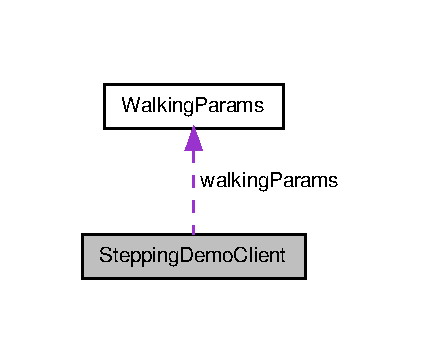
\includegraphics[width=203pt]{classSteppingDemoClient__coll__graph}
\end{center}
\end{figure}
\subsection*{\-Public \-Member \-Functions}
\begin{DoxyCompactItemize}
\item 
\hyperlink{classSteppingDemoClient_a28e41547ba5641741ceb3b378a5983db}{\-Stepping\-Demo\-Client} (std\-::shared\-\_\-ptr$<$ ocra\-::\-Model $>$ model\-Ptr, const int loop\-Period)
\item 
virtual \hyperlink{classSteppingDemoClient_a573eed904c7262c5cdbaf6e254d72559}{$\sim$\-Stepping\-Demo\-Client} ()
\end{DoxyCompactItemize}
\subsection*{\-Public \-Attributes}
\begin{DoxyCompactItemize}
\item 
\hyperlink{SteppingDemoClient_8h_abd6d177d63e98aa1b4ed4b8329e2a379}{\-M\-O\-T\-I\-O\-N\-\_\-\-T\-Y\-P\-E} \hyperlink{classSteppingDemoClient_aa880debbcbed0298ae1769dd8a3f721b}{motion\-Type}
\end{DoxyCompactItemize}
\subsection*{\-Protected \-Member \-Functions}
\begin{DoxyCompactItemize}
\item 
virtual bool \hyperlink{classSteppingDemoClient_a08dce195eece162eed175ac9487667c2}{initialize} ()
\item 
virtual void \hyperlink{classSteppingDemoClient_aafcb227c0d7ce24823957e2331caa88b}{release} ()
\item 
virtual void \hyperlink{classSteppingDemoClient_a37dba4764b5849cf33c395cd0d4b0eb5}{loop} ()
\end{DoxyCompactItemize}
\subsection*{\-Private \-Member \-Functions}
\begin{DoxyCompactItemize}
\item 
void \hyperlink{classSteppingDemoClient_a0f6b689c5f032351484b03e71a3530e1}{static\-Walking\-Loop} ()
\item 
void \hyperlink{classSteppingDemoClient_a94b990ae53b1b40ef8f9469b427d171c}{left\-To\-Right\-Loop} ()
\item 
\-Eigen\-::\-Vector3d \hyperlink{classSteppingDemoClient_af6a814243828f5136476aa5e99ea0079}{get\-Left\-Foot\-Position} ()
\item 
\-Eigen\-::\-Vector3d \hyperlink{classSteppingDemoClient_ae9c0d72756c109f49c269a7e1b06454a}{get\-Right\-Foot\-Position} ()
\item 
\-Eigen\-::\-Vector3d \hyperlink{classSteppingDemoClient_a857aa530a4ab94443d0b0869121baf76}{get\-Co\-M\-Position} ()
\item 
void \hyperlink{classSteppingDemoClient_a18609e5634a283423c228106bb0e3a45}{position\-Co\-M\-Over} (\hyperlink{SteppingDemoClient_8h_ac0c3848a609566394821d9826e0fdd5b}{\-C\-O\-M\-\_\-\-S\-U\-P\-P\-O\-R\-T\-\_\-\-P\-O\-S\-I\-T\-I\-O\-N} new\-Support\-Pos)
\item 
bool \hyperlink{classSteppingDemoClient_ad8fbc186267a47a73bb77e78199f2b8c}{is\-Balanced} ()
\item 
void \hyperlink{classSteppingDemoClient_a62b5028bdc99de117cfffc576478a0f1}{deactivate\-Foot\-Contacts} (\hyperlink{SteppingDemoClient_8h_ab0673d7f17cdd57b8fa124abb330287f}{\-F\-O\-O\-T\-\_\-\-C\-O\-N\-T\-A\-C\-T\-S} foot)
\item 
void \hyperlink{classSteppingDemoClient_abf583698c8c03620516acf3ec6eb9e41}{activate\-Foot\-Contacts} (\hyperlink{SteppingDemoClient_8h_ab0673d7f17cdd57b8fa124abb330287f}{\-F\-O\-O\-T\-\_\-\-C\-O\-N\-T\-A\-C\-T\-S} foot)
\item 
bool \hyperlink{classSteppingDemoClient_aeeaa9fac47e3e5a141647b07fa2feaa3}{is\-Foot\-In\-Contact} (\hyperlink{SteppingDemoClient_8h_ab0673d7f17cdd57b8fa124abb330287f}{\-F\-O\-O\-T\-\_\-\-C\-O\-N\-T\-A\-C\-T\-S} foot)
\item 
void \hyperlink{classSteppingDemoClient_a6b5d8bf0ce08c8b9f66ac2c1bbd5bcd7}{pause\-For} (double \-\_\-pause\-Duration)
\item 
bool \hyperlink{classSteppingDemoClient_afe78b799d8b8c63cff7d1e8765b7e1fa}{pause\-Finished} ()
\item 
bool \hyperlink{classSteppingDemoClient_ae406e5c8f755f234272b63de4d6a774f}{lift\-Foot} (\hyperlink{SteppingDemoClient_8h_ab0673d7f17cdd57b8fa124abb330287f}{\-F\-O\-O\-T\-\_\-\-C\-O\-N\-T\-A\-C\-T\-S} foot, bool is\-Left\-Foot\-In\-Contact, bool is\-Right\-Foot\-In\-Contact)
\item 
bool \hyperlink{classSteppingDemoClient_a930123dad5658ea8a3bb5f23cb4cb369}{set\-Down\-Foot} (\hyperlink{SteppingDemoClient_8h_ab0673d7f17cdd57b8fa124abb330287f}{\-F\-O\-O\-T\-\_\-\-C\-O\-N\-T\-A\-C\-T\-S} foot)
\item 
void \hyperlink{classSteppingDemoClient_a346a8fd10641897532a26f598db7799d}{state\-Machine\-With\-Pause\-In\-Double\-Support} ()
\item 
void \hyperlink{classSteppingDemoClient_a256284578a6b9818a8f726451d2fb2c4}{state\-Machine\-Without\-Pause\-In\-Double\-Support} ()
\end{DoxyCompactItemize}
\subsection*{\-Private \-Attributes}
\begin{DoxyCompactItemize}
\item 
ocra\-\_\-recipes\-::\-Task\-Connection\-::\-Ptr \hyperlink{classSteppingDemoClient_a5dd71720cd8f7a17d21f74d20b3c23ff}{\-Left\-Foot\-Contact\-\_\-\-Back\-Left}
\item 
ocra\-\_\-recipes\-::\-Task\-Connection\-::\-Ptr \hyperlink{classSteppingDemoClient_a32e69816ec216b3d6502385e2346d22d}{\-Left\-Foot\-Contact\-\_\-\-Front\-Left}
\item 
ocra\-\_\-recipes\-::\-Task\-Connection\-::\-Ptr \hyperlink{classSteppingDemoClient_a946ab9de6d55274e5cb9b9a8743a30b8}{\-Left\-Foot\-Contact\-\_\-\-Back\-Right}
\item 
ocra\-\_\-recipes\-::\-Task\-Connection\-::\-Ptr \hyperlink{classSteppingDemoClient_ae2c0ca1ba0ef69b5f09fd3cd982fb772}{\-Left\-Foot\-Contact\-\_\-\-Front\-Right}
\item 
ocra\-\_\-recipes\-::\-Task\-Connection\-::\-Ptr \hyperlink{classSteppingDemoClient_aaaf5dee15bf151def4b4070751d1ca84}{\-Right\-Foot\-Contact\-\_\-\-Back\-Left}
\item 
ocra\-\_\-recipes\-::\-Task\-Connection\-::\-Ptr \hyperlink{classSteppingDemoClient_ad10f639e025b003fd383f4cc933da15f}{\-Right\-Foot\-Contact\-\_\-\-Front\-Left}
\item 
ocra\-\_\-recipes\-::\-Task\-Connection\-::\-Ptr \hyperlink{classSteppingDemoClient_a93e209732588c3ef2b04e39e3df40d3e}{\-Right\-Foot\-Contact\-\_\-\-Back\-Right}
\item 
ocra\-\_\-recipes\-::\-Task\-Connection\-::\-Ptr \hyperlink{classSteppingDemoClient_a781be1c0ffd7e7147eb2b2de66ba3231}{\-Right\-Foot\-Contact\-\_\-\-Front\-Right}
\item 
double \hyperlink{classSteppingDemoClient_a13a5deff16d52936f788bb9b0af6e9c9}{pause\-Trigger\-Time}
\item 
double \hyperlink{classSteppingDemoClient_a92b810b2d2c50e359da18e5d91163340}{pause\-Duration}
\item 
double \hyperlink{classSteppingDemoClient_a1bb7d42cf09778349ae1ecd31d2ac116}{current\-Time}
\item 
bool \hyperlink{classSteppingDemoClient_a29e7765300c7d2e2d5108025fbdcbc2c}{is\-Pausing}
\item 
bool \hyperlink{classSteppingDemoClient_a88b84ed8fc7808ea3fb68f2ec3d29ebe}{is\-In\-Left\-Support\-Mode}
\item 
bool \hyperlink{classSteppingDemoClient_a7697070e5db6c635aa2eff70bce29176}{is\-In\-Right\-Support\-Mode}
\item 
bool \hyperlink{classSteppingDemoClient_a6036e2d0b604648ca39e4d64b41a9d6e}{foot\-Trajectory\-Started}
\item 
std\-::shared\-\_\-ptr\*
$<$ ocra\-\_\-recipes\-::\-Trajectory\-Thread $>$ \hyperlink{classSteppingDemoClient_afd18627088c2c12f172ff9e976da5330}{left\-Foot\-\_\-\-Traj\-Thread}
\item 
std\-::shared\-\_\-ptr\*
$<$ ocra\-\_\-recipes\-::\-Trajectory\-Thread $>$ \hyperlink{classSteppingDemoClient_a8b4b931d41b47d9923417506fac107f3}{right\-Foot\-\_\-\-Traj\-Thread}
\item 
std\-::shared\-\_\-ptr\*
$<$ ocra\-\_\-recipes\-::\-Trajectory\-Thread $>$ \hyperlink{classSteppingDemoClient_a9f3d1cdc49cc26a10f9b8fb0d0c68cab}{com\-\_\-\-Traj\-Thread}
\item 
\-Eigen\-::\-Vector3d \hyperlink{classSteppingDemoClient_acd4cb9dbe053979701574f5d1d4ef349}{left\-Foot\-Home}
\item 
\-Eigen\-::\-Vector3d \hyperlink{classSteppingDemoClient_ae2a3bdaafc7784b5afece8ae9ebaff7d}{right\-Foot\-Home}
\item 
\-Eigen\-::\-Vector3d \hyperlink{classSteppingDemoClient_aa018c1f2734d63f962be512461c9e010}{com\-Home}
\item 
\-Eigen\-::\-Vector3d \hyperlink{classSteppingDemoClient_a2360933e2902d1b1a374787bd67e14e7}{left\-Foot\-Target}
\item 
\-Eigen\-::\-Vector3d \hyperlink{classSteppingDemoClient_abfe6635a0ad50fa4baa6fa10b8c56d9e}{right\-Foot\-Target}
\item 
\-Eigen\-::\-Vector3d \hyperlink{classSteppingDemoClient_af9e0358390f12ed0135275b20bf1f6f5}{next\-Step}
\item 
\-Eigen\-::\-Vector3d \hyperlink{classSteppingDemoClient_ab4a77111abbf3630280a64d17ac59eef}{new\-Co\-M\-Goal\-Position}
\item 
double \hyperlink{classSteppingDemoClient_af7b6e48319ef9d35fb975edc3bb2a137}{start\-Time}
\item 
bool \hyperlink{classSteppingDemoClient_aedd8bb5bca60afbdd2b8de3b5d1829d7}{get\-Initial\-Values}
\item 
\hyperlink{SteppingDemoClient_8h_af2a8507bf21c3ce9b0e67a23381251c6}{\-C\-O\-N\-T\-R\-O\-L\-\_\-\-P\-H\-A\-S\-E} \hyperlink{classSteppingDemoClient_afe0aa2a02ea8117d644bf5444a03ac62}{current\-Phase}
\item 
\hyperlink{SteppingDemoClient_8h_af2a8507bf21c3ce9b0e67a23381251c6}{\-C\-O\-N\-T\-R\-O\-L\-\_\-\-P\-H\-A\-S\-E} \hyperlink{classSteppingDemoClient_ab5a3b82049a9786162a60d0ae94f96d9}{next\-Phase}
\item 
bool \hyperlink{classSteppingDemoClient_ad7e3950d053af7c1aca33b3e7c3b20c5}{is\-Moving\-Co\-M}
\item 
\hyperlink{structWalkingParams}{\-Walking\-Params} \hyperlink{classSteppingDemoClient_a113c2d838e3db1d18f4843a8828e30d4}{walking\-Params}
\end{DoxyCompactItemize}


\subsection{\-Constructor \& \-Destructor \-Documentation}
\hypertarget{classSteppingDemoClient_a28e41547ba5641741ceb3b378a5983db}{\index{\-Stepping\-Demo\-Client@{\-Stepping\-Demo\-Client}!\-Stepping\-Demo\-Client@{\-Stepping\-Demo\-Client}}
\index{\-Stepping\-Demo\-Client@{\-Stepping\-Demo\-Client}!SteppingDemoClient@{\-Stepping\-Demo\-Client}}
\subsubsection[{\-Stepping\-Demo\-Client}]{\setlength{\rightskip}{0pt plus 5cm}{\bf \-Stepping\-Demo\-Client\-::\-Stepping\-Demo\-Client} (
\begin{DoxyParamCaption}
\item[{std\-::shared\-\_\-ptr$<$ ocra\-::\-Model $>$}]{model\-Ptr, }
\item[{const int}]{loop\-Period}
\end{DoxyParamCaption}
)}}\label{classSteppingDemoClient_a28e41547ba5641741ceb3b378a5983db}
\hypertarget{classSteppingDemoClient_a573eed904c7262c5cdbaf6e254d72559}{\index{\-Stepping\-Demo\-Client@{\-Stepping\-Demo\-Client}!$\sim$\-Stepping\-Demo\-Client@{$\sim$\-Stepping\-Demo\-Client}}
\index{$\sim$\-Stepping\-Demo\-Client@{$\sim$\-Stepping\-Demo\-Client}!SteppingDemoClient@{\-Stepping\-Demo\-Client}}
\subsubsection[{$\sim$\-Stepping\-Demo\-Client}]{\setlength{\rightskip}{0pt plus 5cm}{\bf \-Stepping\-Demo\-Client\-::$\sim$\-Stepping\-Demo\-Client} (
\begin{DoxyParamCaption}
{}
\end{DoxyParamCaption}
)\hspace{0.3cm}{\ttfamily  \mbox{[}virtual\mbox{]}}}}\label{classSteppingDemoClient_a573eed904c7262c5cdbaf6e254d72559}


\subsection{\-Member \-Function \-Documentation}
\hypertarget{classSteppingDemoClient_abf583698c8c03620516acf3ec6eb9e41}{\index{\-Stepping\-Demo\-Client@{\-Stepping\-Demo\-Client}!activate\-Foot\-Contacts@{activate\-Foot\-Contacts}}
\index{activate\-Foot\-Contacts@{activate\-Foot\-Contacts}!SteppingDemoClient@{\-Stepping\-Demo\-Client}}
\subsubsection[{activate\-Foot\-Contacts}]{\setlength{\rightskip}{0pt plus 5cm}void {\bf \-Stepping\-Demo\-Client\-::activate\-Foot\-Contacts} (
\begin{DoxyParamCaption}
\item[{{\bf \-F\-O\-O\-T\-\_\-\-C\-O\-N\-T\-A\-C\-T\-S}}]{foot}
\end{DoxyParamCaption}
)\hspace{0.3cm}{\ttfamily  \mbox{[}private\mbox{]}}}}\label{classSteppingDemoClient_abf583698c8c03620516acf3ec6eb9e41}
\-This method asks the ocra-\/icub-\/server to activate one by one the feet \char`\"{}corner\char`\"{} contact tasks for the specified foot.


\begin{DoxyParams}{\-Parameters}
{\em foot} & \-L\-E\-F\-T\-\_\-\-F\-O\-O\-T or \-R\-I\-G\-H\-T\-\_\-\-F\-O\-O\-T. \\
\hline
\end{DoxyParams}
\hypertarget{classSteppingDemoClient_a62b5028bdc99de117cfffc576478a0f1}{\index{\-Stepping\-Demo\-Client@{\-Stepping\-Demo\-Client}!deactivate\-Foot\-Contacts@{deactivate\-Foot\-Contacts}}
\index{deactivate\-Foot\-Contacts@{deactivate\-Foot\-Contacts}!SteppingDemoClient@{\-Stepping\-Demo\-Client}}
\subsubsection[{deactivate\-Foot\-Contacts}]{\setlength{\rightskip}{0pt plus 5cm}void {\bf \-Stepping\-Demo\-Client\-::deactivate\-Foot\-Contacts} (
\begin{DoxyParamCaption}
\item[{{\bf \-F\-O\-O\-T\-\_\-\-C\-O\-N\-T\-A\-C\-T\-S}}]{foot}
\end{DoxyParamCaption}
)\hspace{0.3cm}{\ttfamily  \mbox{[}private\mbox{]}}}}\label{classSteppingDemoClient_a62b5028bdc99de117cfffc576478a0f1}
\-Remember the right and left feet contact tasks? created in \hyperlink{classSteppingDemoClient_a08dce195eece162eed175ac9487667c2}{initialize()}. \-This method acts the ocra-\/icub-\/server to deactivate one by one the feet \char`\"{}corner\char`\"{} contact tasks for the specified foot.


\begin{DoxyParams}{\-Parameters}
{\em foot} & \-L\-E\-F\-T\-\_\-\-F\-O\-O\-T or \-R\-I\-G\-H\-T\-\_\-\-F\-O\-O\-T. \\
\hline
\end{DoxyParams}
\hypertarget{classSteppingDemoClient_a857aa530a4ab94443d0b0869121baf76}{\index{\-Stepping\-Demo\-Client@{\-Stepping\-Demo\-Client}!get\-Co\-M\-Position@{get\-Co\-M\-Position}}
\index{get\-Co\-M\-Position@{get\-Co\-M\-Position}!SteppingDemoClient@{\-Stepping\-Demo\-Client}}
\subsubsection[{get\-Co\-M\-Position}]{\setlength{\rightskip}{0pt plus 5cm}\-Eigen\-::\-Vector3d {\bf \-Stepping\-Demo\-Client\-::get\-Co\-M\-Position} (
\begin{DoxyParamCaption}
{}
\end{DoxyParamCaption}
)\hspace{0.3cm}{\ttfamily  \mbox{[}private\mbox{]}}}}\label{classSteppingDemoClient_a857aa530a4ab94443d0b0869121baf76}
\-Retrieves the 3\-D position of the \char`\"{}\-Co\-M\char`\"{} as done by the yarp\-Whole\-Body\-Interface.

\begin{DoxyReturn}{\-Returns}
3\-D position of the \-C\-O\-M. 
\end{DoxyReturn}
\hypertarget{classSteppingDemoClient_af6a814243828f5136476aa5e99ea0079}{\index{\-Stepping\-Demo\-Client@{\-Stepping\-Demo\-Client}!get\-Left\-Foot\-Position@{get\-Left\-Foot\-Position}}
\index{get\-Left\-Foot\-Position@{get\-Left\-Foot\-Position}!SteppingDemoClient@{\-Stepping\-Demo\-Client}}
\subsubsection[{get\-Left\-Foot\-Position}]{\setlength{\rightskip}{0pt plus 5cm}\-Eigen\-::\-Vector3d {\bf \-Stepping\-Demo\-Client\-::get\-Left\-Foot\-Position} (
\begin{DoxyParamCaption}
{}
\end{DoxyParamCaption}
)\hspace{0.3cm}{\ttfamily  \mbox{[}private\mbox{]}}}}\label{classSteppingDemoClient_af6a814243828f5136476aa5e99ea0079}
\-Retrieves the 3\-D position of the \char`\"{}l\-\_\-sole\char`\"{} frame from the i\-Cub model.

\begin{DoxyReturn}{\-Returns}
3\-D position of the left foot. 
\end{DoxyReturn}
\hypertarget{classSteppingDemoClient_ae9c0d72756c109f49c269a7e1b06454a}{\index{\-Stepping\-Demo\-Client@{\-Stepping\-Demo\-Client}!get\-Right\-Foot\-Position@{get\-Right\-Foot\-Position}}
\index{get\-Right\-Foot\-Position@{get\-Right\-Foot\-Position}!SteppingDemoClient@{\-Stepping\-Demo\-Client}}
\subsubsection[{get\-Right\-Foot\-Position}]{\setlength{\rightskip}{0pt plus 5cm}\-Eigen\-::\-Vector3d {\bf \-Stepping\-Demo\-Client\-::get\-Right\-Foot\-Position} (
\begin{DoxyParamCaption}
{}
\end{DoxyParamCaption}
)\hspace{0.3cm}{\ttfamily  \mbox{[}private\mbox{]}}}}\label{classSteppingDemoClient_ae9c0d72756c109f49c269a7e1b06454a}
\-Retrieves the 3\-D position of the \char`\"{}r\-\_\-sole\char`\"{} frame from the i\-Cub model.

\begin{DoxyReturn}{\-Returns}
3\-D position of the right foot. 
\end{DoxyReturn}
\hypertarget{classSteppingDemoClient_a08dce195eece162eed175ac9487667c2}{\index{\-Stepping\-Demo\-Client@{\-Stepping\-Demo\-Client}!initialize@{initialize}}
\index{initialize@{initialize}!SteppingDemoClient@{\-Stepping\-Demo\-Client}}
\subsubsection[{initialize}]{\setlength{\rightskip}{0pt plus 5cm}bool {\bf \-Stepping\-Demo\-Client\-::initialize} (
\begin{DoxyParamCaption}
{}
\end{DoxyParamCaption}
)\hspace{0.3cm}{\ttfamily  \mbox{[}protected, virtual\mbox{]}}}}\label{classSteppingDemoClient_a08dce195eece162eed175ac9487667c2}
\-The initialization consists of the following\-: 1. \-Defines trajectory types (e.\-g. \-Min. \-Jerk) 2. \-Defines the termination strategy 3. \-Instantiates trajectory threads for the left and right foot as well as for the \-Co\-M, sets them up (max velocity, error threshold) and finally starts them. 4. \-Instantiates ocra\-::\-Task\-Connection objects for the left and right feet contacts (4 per foot on each corner).


\begin{DoxyItemize}
\item returns\-: \-True if everything has been initialized properly, false otherwise. 
\end{DoxyItemize}\hypertarget{classSteppingDemoClient_ad8fbc186267a47a73bb77e78199f2b8c}{\index{\-Stepping\-Demo\-Client@{\-Stepping\-Demo\-Client}!is\-Balanced@{is\-Balanced}}
\index{is\-Balanced@{is\-Balanced}!SteppingDemoClient@{\-Stepping\-Demo\-Client}}
\subsubsection[{is\-Balanced}]{\setlength{\rightskip}{0pt plus 5cm}bool {\bf \-Stepping\-Demo\-Client\-::is\-Balanced} (
\begin{DoxyParamCaption}
{}
\end{DoxyParamCaption}
)\hspace{0.3cm}{\ttfamily  \mbox{[}private\mbox{]}}}}\label{classSteppingDemoClient_ad8fbc186267a47a73bb77e78199f2b8c}
\-Uses the norm of the \-C\-O\-M and joint velocities to understand if the robot is balanced.

\begin{DoxyReturn}{\-Returns}
\-True when both the norm of the \-C\-O\-M and joint velocities are below com\-Vel\-Threshold and joint\-Threshold. 
\end{DoxyReturn}
\begin{DoxyRefDesc}{\-Todo}
\item[\hyperlink{todo__todo000002}{\-Todo}]\-A more balance-\/centered criterion should be used for this, \-Z\-M\-P-\/based for example. \end{DoxyRefDesc}
\hypertarget{classSteppingDemoClient_aeeaa9fac47e3e5a141647b07fa2feaa3}{\index{\-Stepping\-Demo\-Client@{\-Stepping\-Demo\-Client}!is\-Foot\-In\-Contact@{is\-Foot\-In\-Contact}}
\index{is\-Foot\-In\-Contact@{is\-Foot\-In\-Contact}!SteppingDemoClient@{\-Stepping\-Demo\-Client}}
\subsubsection[{is\-Foot\-In\-Contact}]{\setlength{\rightskip}{0pt plus 5cm}bool {\bf \-Stepping\-Demo\-Client\-::is\-Foot\-In\-Contact} (
\begin{DoxyParamCaption}
\item[{{\bf \-F\-O\-O\-T\-\_\-\-C\-O\-N\-T\-A\-C\-T\-S}}]{foot}
\end{DoxyParamCaption}
)\hspace{0.3cm}{\ttfamily  \mbox{[}private\mbox{]}}}}\label{classSteppingDemoClient_aeeaa9fac47e3e5a141647b07fa2feaa3}
\-If the foot height is less than or equal to foot\-Contact\-Release\-Threshold, the feet contacts tasks are activated.


\begin{DoxyParams}{\-Parameters}
{\em foot} & \-L\-E\-F\-T\-\_\-\-F\-O\-O\-T or \-R\-I\-G\-H\-T\-\_\-\-F\-O\-O\-T.\\
\hline
\end{DoxyParams}
\begin{DoxyReturn}{\-Returns}
\-True if the activation of the contact happens successfully. \-False if the foot's elevation is not under the foot\-Contact\-Release\-Threshold. 
\end{DoxyReturn}
\hypertarget{classSteppingDemoClient_a94b990ae53b1b40ef8f9469b427d171c}{\index{\-Stepping\-Demo\-Client@{\-Stepping\-Demo\-Client}!left\-To\-Right\-Loop@{left\-To\-Right\-Loop}}
\index{left\-To\-Right\-Loop@{left\-To\-Right\-Loop}!SteppingDemoClient@{\-Stepping\-Demo\-Client}}
\subsubsection[{left\-To\-Right\-Loop}]{\setlength{\rightskip}{0pt plus 5cm}void {\bf \-Stepping\-Demo\-Client\-::left\-To\-Right\-Loop} (
\begin{DoxyParamCaption}
{}
\end{DoxyParamCaption}
)\hspace{0.3cm}{\ttfamily  \mbox{[}private\mbox{]}}}}\label{classSteppingDemoClient_a94b990ae53b1b40ef8f9469b427d171c}
\hypertarget{classSteppingDemoClient_ae406e5c8f755f234272b63de4d6a774f}{\index{\-Stepping\-Demo\-Client@{\-Stepping\-Demo\-Client}!lift\-Foot@{lift\-Foot}}
\index{lift\-Foot@{lift\-Foot}!SteppingDemoClient@{\-Stepping\-Demo\-Client}}
\subsubsection[{lift\-Foot}]{\setlength{\rightskip}{0pt plus 5cm}bool {\bf \-Stepping\-Demo\-Client\-::lift\-Foot} (
\begin{DoxyParamCaption}
\item[{{\bf \-F\-O\-O\-T\-\_\-\-C\-O\-N\-T\-A\-C\-T\-S}}]{foot, }
\item[{bool}]{is\-Left\-Foot\-In\-Contact, }
\item[{bool}]{is\-Right\-Foot\-In\-Contact}
\end{DoxyParamCaption}
)\hspace{0.3cm}{\ttfamily  \mbox{[}private\mbox{]}}}}\label{classSteppingDemoClient_ae406e5c8f755f234272b63de4d6a774f}
\-Sets the right or left foot waypoint to right\-Foot\-Target or left\-Foot\-Target accordingly (where the foot will be lifted). \-These values are harcoded in the \hyperlink{classSteppingDemoClient_a37dba4764b5849cf33c395cd0d4b0eb5}{loop()} method and updated only during the very first iteration when the variable get\-Initial\-Values is set to true.


\begin{DoxyParams}{\-Parameters}
{\em foot} & \-L\-E\-F\-T\-\_\-\-F\-O\-O\-T or \-R\-I\-G\-H\-T\-\_\-\-F\-O\-O\-T \\
\hline
{\em is\-Left\-Foot\-In\-Contact} & \-Updates the current state of the left foot contact. \\
\hline
{\em is\-Right\-Foot\-In\-Contact} & \-Updates the current state of the right foot contact.\\
\hline
\end{DoxyParams}
\begin{DoxyReturn}{\-Returns}
\-True after the foot contact is deactivated. 
\end{DoxyReturn}
\hypertarget{classSteppingDemoClient_a37dba4764b5849cf33c395cd0d4b0eb5}{\index{\-Stepping\-Demo\-Client@{\-Stepping\-Demo\-Client}!loop@{loop}}
\index{loop@{loop}!SteppingDemoClient@{\-Stepping\-Demo\-Client}}
\subsubsection[{loop}]{\setlength{\rightskip}{0pt plus 5cm}void {\bf \-Stepping\-Demo\-Client\-::loop} (
\begin{DoxyParamCaption}
{}
\end{DoxyParamCaption}
)\hspace{0.3cm}{\ttfamily  \mbox{[}protected, virtual\mbox{]}}}}\label{classSteppingDemoClient_a37dba4764b5849cf33c395cd0d4b0eb5}
\-Initially waits for two seconds, to make sure that all model states have been correctly updated during the initialization. \-During the first loop it retrieves left and right feet positions along with the com's. \hypertarget{classSteppingDemoClient_afe78b799d8b8c63cff7d1e8765b7e1fa}{\index{\-Stepping\-Demo\-Client@{\-Stepping\-Demo\-Client}!pause\-Finished@{pause\-Finished}}
\index{pause\-Finished@{pause\-Finished}!SteppingDemoClient@{\-Stepping\-Demo\-Client}}
\subsubsection[{pause\-Finished}]{\setlength{\rightskip}{0pt plus 5cm}bool {\bf \-Stepping\-Demo\-Client\-::pause\-Finished} (
\begin{DoxyParamCaption}
{}
\end{DoxyParamCaption}
)\hspace{0.3cm}{\ttfamily  \mbox{[}private\mbox{]}}}}\label{classSteppingDemoClient_afe78b799d8b8c63cff7d1e8765b7e1fa}
\-Sets is\-Pausing to false when pause\-Duration has passed.

\begin{DoxyReturn}{\-Returns}
\-True when the pause duration is over. \-False otherwise. 
\end{DoxyReturn}
\hypertarget{classSteppingDemoClient_a6b5d8bf0ce08c8b9f66ac2c1bbd5bcd7}{\index{\-Stepping\-Demo\-Client@{\-Stepping\-Demo\-Client}!pause\-For@{pause\-For}}
\index{pause\-For@{pause\-For}!SteppingDemoClient@{\-Stepping\-Demo\-Client}}
\subsubsection[{pause\-For}]{\setlength{\rightskip}{0pt plus 5cm}void {\bf \-Stepping\-Demo\-Client\-::pause\-For} (
\begin{DoxyParamCaption}
\item[{double}]{\-\_\-pause\-Duration}
\end{DoxyParamCaption}
)\hspace{0.3cm}{\ttfamily  \mbox{[}private\mbox{]}}}}\label{classSteppingDemoClient_a6b5d8bf0ce08c8b9f66ac2c1bbd5bcd7}
\-Mainly sets is\-Pausing to true and stores the time at which the pause was called.


\begin{DoxyParams}{\-Parameters}
{\em \-\_\-pause\-Duration} & \-Pause duration. \\
\hline
\end{DoxyParams}
\hypertarget{classSteppingDemoClient_a18609e5634a283423c228106bb0e3a45}{\index{\-Stepping\-Demo\-Client@{\-Stepping\-Demo\-Client}!position\-Co\-M\-Over@{position\-Co\-M\-Over}}
\index{position\-Co\-M\-Over@{position\-Co\-M\-Over}!SteppingDemoClient@{\-Stepping\-Demo\-Client}}
\subsubsection[{position\-Co\-M\-Over}]{\setlength{\rightskip}{0pt plus 5cm}void {\bf \-Stepping\-Demo\-Client\-::position\-Co\-M\-Over} (
\begin{DoxyParamCaption}
\item[{{\bf \-C\-O\-M\-\_\-\-S\-U\-P\-P\-O\-R\-T\-\_\-\-P\-O\-S\-I\-T\-I\-O\-N}}]{new\-Support\-Pos}
\end{DoxyParamCaption}
)\hspace{0.3cm}{\ttfamily  \mbox{[}private\mbox{]}}}}\label{classSteppingDemoClient_a18609e5634a283423c228106bb0e3a45}
\-Sets \-C\-O\-M trajectory waypoints according to the desired support position\-: \-L\-E\-F\-T\-\_\-\-F\-O\-O\-T\-\_\-\-X\-Y\-: \-The \-C\-O\-M goal position is set to be on top of the left foot. \-R\-I\-G\-H\-T\-\_\-\-F\-O\-O\-T\-\_\-\-X\-Y\-: \-The \-C\-O\-M goal position is set to be on top of the right foot. \-C\-E\-N\-T\-E\-R\-E\-D\-\_\-\-B\-E\-T\-W\-E\-E\-N\-\_\-\-F\-E\-E\-T\-\_\-\-X\-Y\-: \-The \-C\-O\-M goal position is set between both feet. \-The height of the com is always the current \-C\-O\-M's height. \-Since the thread must have started before calling this method, it will update the current waypoint trajectory it has or start it.


\begin{DoxyParams}{\-Parameters}
{\em new\-Support\-Pos} & \-New support position. \\
\hline
\end{DoxyParams}
\hypertarget{classSteppingDemoClient_aafcb227c0d7ce24823957e2331caa88b}{\index{\-Stepping\-Demo\-Client@{\-Stepping\-Demo\-Client}!release@{release}}
\index{release@{release}!SteppingDemoClient@{\-Stepping\-Demo\-Client}}
\subsubsection[{release}]{\setlength{\rightskip}{0pt plus 5cm}void {\bf \-Stepping\-Demo\-Client\-::release} (
\begin{DoxyParamCaption}
{}
\end{DoxyParamCaption}
)\hspace{0.3cm}{\ttfamily  \mbox{[}protected, virtual\mbox{]}}}}\label{classSteppingDemoClient_aafcb227c0d7ce24823957e2331caa88b}
\-Stops the trajectory threads of the \-Co\-M, left and right feet. \hypertarget{classSteppingDemoClient_a930123dad5658ea8a3bb5f23cb4cb369}{\index{\-Stepping\-Demo\-Client@{\-Stepping\-Demo\-Client}!set\-Down\-Foot@{set\-Down\-Foot}}
\index{set\-Down\-Foot@{set\-Down\-Foot}!SteppingDemoClient@{\-Stepping\-Demo\-Client}}
\subsubsection[{set\-Down\-Foot}]{\setlength{\rightskip}{0pt plus 5cm}bool {\bf \-Stepping\-Demo\-Client\-::set\-Down\-Foot} (
\begin{DoxyParamCaption}
\item[{{\bf \-F\-O\-O\-T\-\_\-\-C\-O\-N\-T\-A\-C\-T\-S}}]{foot}
\end{DoxyParamCaption}
)\hspace{0.3cm}{\ttfamily  \mbox{[}private\mbox{]}}}}\label{classSteppingDemoClient_a930123dad5658ea8a3bb5f23cb4cb369}
\-Sets the right or left foot waypoint to right\-Foot\-Home or left\-Foot\-Home accordingly (where the foot will land). \-These values are harcoded in the \hyperlink{classSteppingDemoClient_a37dba4764b5849cf33c395cd0d4b0eb5}{loop()} method and updated only during the very first iteration when the variable get\-Initial\-Values is set to true.


\begin{DoxyParams}{\-Parameters}
{\em foot} & \-L\-E\-F\-T\-\_\-\-F\-O\-O\-T or \-R\-I\-G\-H\-T\-\_\-\-F\-O\-O\-T\\
\hline
\end{DoxyParams}
\begin{DoxyReturn}{\-Returns}
\-True only after the foot has established contact again and the trajectory is over. \-False while the foot is still moving back down looking for contact or simply, the goal hasn't been attained. 
\end{DoxyReturn}
\hypertarget{classSteppingDemoClient_a256284578a6b9818a8f726451d2fb2c4}{\index{\-Stepping\-Demo\-Client@{\-Stepping\-Demo\-Client}!state\-Machine\-Without\-Pause\-In\-Double\-Support@{state\-Machine\-Without\-Pause\-In\-Double\-Support}}
\index{state\-Machine\-Without\-Pause\-In\-Double\-Support@{state\-Machine\-Without\-Pause\-In\-Double\-Support}!SteppingDemoClient@{\-Stepping\-Demo\-Client}}
\subsubsection[{state\-Machine\-Without\-Pause\-In\-Double\-Support}]{\setlength{\rightskip}{0pt plus 5cm}void {\bf \-Stepping\-Demo\-Client\-::state\-Machine\-Without\-Pause\-In\-Double\-Support} (
\begin{DoxyParamCaption}
{}
\end{DoxyParamCaption}
)\hspace{0.3cm}{\ttfamily  \mbox{[}private\mbox{]}}}}\label{classSteppingDemoClient_a256284578a6b9818a8f726451d2fb2c4}
\hypertarget{classSteppingDemoClient_a346a8fd10641897532a26f598db7799d}{\index{\-Stepping\-Demo\-Client@{\-Stepping\-Demo\-Client}!state\-Machine\-With\-Pause\-In\-Double\-Support@{state\-Machine\-With\-Pause\-In\-Double\-Support}}
\index{state\-Machine\-With\-Pause\-In\-Double\-Support@{state\-Machine\-With\-Pause\-In\-Double\-Support}!SteppingDemoClient@{\-Stepping\-Demo\-Client}}
\subsubsection[{state\-Machine\-With\-Pause\-In\-Double\-Support}]{\setlength{\rightskip}{0pt plus 5cm}void {\bf \-Stepping\-Demo\-Client\-::state\-Machine\-With\-Pause\-In\-Double\-Support} (
\begin{DoxyParamCaption}
{}
\end{DoxyParamCaption}
)\hspace{0.3cm}{\ttfamily  \mbox{[}private\mbox{]}}}}\label{classSteppingDemoClient_a346a8fd10641897532a26f598db7799d}
\hypertarget{classSteppingDemoClient_a0f6b689c5f032351484b03e71a3530e1}{\index{\-Stepping\-Demo\-Client@{\-Stepping\-Demo\-Client}!static\-Walking\-Loop@{static\-Walking\-Loop}}
\index{static\-Walking\-Loop@{static\-Walking\-Loop}!SteppingDemoClient@{\-Stepping\-Demo\-Client}}
\subsubsection[{static\-Walking\-Loop}]{\setlength{\rightskip}{0pt plus 5cm}void {\bf \-Stepping\-Demo\-Client\-::static\-Walking\-Loop} (
\begin{DoxyParamCaption}
{}
\end{DoxyParamCaption}
)\hspace{0.3cm}{\ttfamily  \mbox{[}private\mbox{]}}}}\label{classSteppingDemoClient_a0f6b689c5f032351484b03e71a3530e1}


\subsection{\-Member \-Data \-Documentation}
\hypertarget{classSteppingDemoClient_a9f3d1cdc49cc26a10f9b8fb0d0c68cab}{\index{\-Stepping\-Demo\-Client@{\-Stepping\-Demo\-Client}!com\-\_\-\-Traj\-Thread@{com\-\_\-\-Traj\-Thread}}
\index{com\-\_\-\-Traj\-Thread@{com\-\_\-\-Traj\-Thread}!SteppingDemoClient@{\-Stepping\-Demo\-Client}}
\subsubsection[{com\-\_\-\-Traj\-Thread}]{\setlength{\rightskip}{0pt plus 5cm}std\-::shared\-\_\-ptr$<$ocra\-\_\-recipes\-::\-Trajectory\-Thread$>$ {\bf \-Stepping\-Demo\-Client\-::com\-\_\-\-Traj\-Thread}\hspace{0.3cm}{\ttfamily  \mbox{[}private\mbox{]}}}}\label{classSteppingDemoClient_a9f3d1cdc49cc26a10f9b8fb0d0c68cab}
\hypertarget{classSteppingDemoClient_aa018c1f2734d63f962be512461c9e010}{\index{\-Stepping\-Demo\-Client@{\-Stepping\-Demo\-Client}!com\-Home@{com\-Home}}
\index{com\-Home@{com\-Home}!SteppingDemoClient@{\-Stepping\-Demo\-Client}}
\subsubsection[{com\-Home}]{\setlength{\rightskip}{0pt plus 5cm}\-Eigen\-::\-Vector3d {\bf \-Stepping\-Demo\-Client\-::com\-Home}\hspace{0.3cm}{\ttfamily  \mbox{[}private\mbox{]}}}}\label{classSteppingDemoClient_aa018c1f2734d63f962be512461c9e010}
\hypertarget{classSteppingDemoClient_afe0aa2a02ea8117d644bf5444a03ac62}{\index{\-Stepping\-Demo\-Client@{\-Stepping\-Demo\-Client}!current\-Phase@{current\-Phase}}
\index{current\-Phase@{current\-Phase}!SteppingDemoClient@{\-Stepping\-Demo\-Client}}
\subsubsection[{current\-Phase}]{\setlength{\rightskip}{0pt plus 5cm}{\bf \-C\-O\-N\-T\-R\-O\-L\-\_\-\-P\-H\-A\-S\-E} {\bf \-Stepping\-Demo\-Client\-::current\-Phase}\hspace{0.3cm}{\ttfamily  \mbox{[}private\mbox{]}}}}\label{classSteppingDemoClient_afe0aa2a02ea8117d644bf5444a03ac62}
\hypertarget{classSteppingDemoClient_a1bb7d42cf09778349ae1ecd31d2ac116}{\index{\-Stepping\-Demo\-Client@{\-Stepping\-Demo\-Client}!current\-Time@{current\-Time}}
\index{current\-Time@{current\-Time}!SteppingDemoClient@{\-Stepping\-Demo\-Client}}
\subsubsection[{current\-Time}]{\setlength{\rightskip}{0pt plus 5cm}double {\bf \-Stepping\-Demo\-Client\-::current\-Time}\hspace{0.3cm}{\ttfamily  \mbox{[}private\mbox{]}}}}\label{classSteppingDemoClient_a1bb7d42cf09778349ae1ecd31d2ac116}
\hypertarget{classSteppingDemoClient_a6036e2d0b604648ca39e4d64b41a9d6e}{\index{\-Stepping\-Demo\-Client@{\-Stepping\-Demo\-Client}!foot\-Trajectory\-Started@{foot\-Trajectory\-Started}}
\index{foot\-Trajectory\-Started@{foot\-Trajectory\-Started}!SteppingDemoClient@{\-Stepping\-Demo\-Client}}
\subsubsection[{foot\-Trajectory\-Started}]{\setlength{\rightskip}{0pt plus 5cm}bool {\bf \-Stepping\-Demo\-Client\-::foot\-Trajectory\-Started}\hspace{0.3cm}{\ttfamily  \mbox{[}private\mbox{]}}}}\label{classSteppingDemoClient_a6036e2d0b604648ca39e4d64b41a9d6e}
\hypertarget{classSteppingDemoClient_aedd8bb5bca60afbdd2b8de3b5d1829d7}{\index{\-Stepping\-Demo\-Client@{\-Stepping\-Demo\-Client}!get\-Initial\-Values@{get\-Initial\-Values}}
\index{get\-Initial\-Values@{get\-Initial\-Values}!SteppingDemoClient@{\-Stepping\-Demo\-Client}}
\subsubsection[{get\-Initial\-Values}]{\setlength{\rightskip}{0pt plus 5cm}bool {\bf \-Stepping\-Demo\-Client\-::get\-Initial\-Values}\hspace{0.3cm}{\ttfamily  \mbox{[}private\mbox{]}}}}\label{classSteppingDemoClient_aedd8bb5bca60afbdd2b8de3b5d1829d7}
\hypertarget{classSteppingDemoClient_a88b84ed8fc7808ea3fb68f2ec3d29ebe}{\index{\-Stepping\-Demo\-Client@{\-Stepping\-Demo\-Client}!is\-In\-Left\-Support\-Mode@{is\-In\-Left\-Support\-Mode}}
\index{is\-In\-Left\-Support\-Mode@{is\-In\-Left\-Support\-Mode}!SteppingDemoClient@{\-Stepping\-Demo\-Client}}
\subsubsection[{is\-In\-Left\-Support\-Mode}]{\setlength{\rightskip}{0pt plus 5cm}bool {\bf \-Stepping\-Demo\-Client\-::is\-In\-Left\-Support\-Mode}\hspace{0.3cm}{\ttfamily  \mbox{[}private\mbox{]}}}}\label{classSteppingDemoClient_a88b84ed8fc7808ea3fb68f2ec3d29ebe}
\hypertarget{classSteppingDemoClient_a7697070e5db6c635aa2eff70bce29176}{\index{\-Stepping\-Demo\-Client@{\-Stepping\-Demo\-Client}!is\-In\-Right\-Support\-Mode@{is\-In\-Right\-Support\-Mode}}
\index{is\-In\-Right\-Support\-Mode@{is\-In\-Right\-Support\-Mode}!SteppingDemoClient@{\-Stepping\-Demo\-Client}}
\subsubsection[{is\-In\-Right\-Support\-Mode}]{\setlength{\rightskip}{0pt plus 5cm}bool {\bf \-Stepping\-Demo\-Client\-::is\-In\-Right\-Support\-Mode}\hspace{0.3cm}{\ttfamily  \mbox{[}private\mbox{]}}}}\label{classSteppingDemoClient_a7697070e5db6c635aa2eff70bce29176}
\hypertarget{classSteppingDemoClient_ad7e3950d053af7c1aca33b3e7c3b20c5}{\index{\-Stepping\-Demo\-Client@{\-Stepping\-Demo\-Client}!is\-Moving\-Co\-M@{is\-Moving\-Co\-M}}
\index{is\-Moving\-Co\-M@{is\-Moving\-Co\-M}!SteppingDemoClient@{\-Stepping\-Demo\-Client}}
\subsubsection[{is\-Moving\-Co\-M}]{\setlength{\rightskip}{0pt plus 5cm}bool {\bf \-Stepping\-Demo\-Client\-::is\-Moving\-Co\-M}\hspace{0.3cm}{\ttfamily  \mbox{[}private\mbox{]}}}}\label{classSteppingDemoClient_ad7e3950d053af7c1aca33b3e7c3b20c5}
\hypertarget{classSteppingDemoClient_a29e7765300c7d2e2d5108025fbdcbc2c}{\index{\-Stepping\-Demo\-Client@{\-Stepping\-Demo\-Client}!is\-Pausing@{is\-Pausing}}
\index{is\-Pausing@{is\-Pausing}!SteppingDemoClient@{\-Stepping\-Demo\-Client}}
\subsubsection[{is\-Pausing}]{\setlength{\rightskip}{0pt plus 5cm}bool {\bf \-Stepping\-Demo\-Client\-::is\-Pausing}\hspace{0.3cm}{\ttfamily  \mbox{[}private\mbox{]}}}}\label{classSteppingDemoClient_a29e7765300c7d2e2d5108025fbdcbc2c}
\hypertarget{classSteppingDemoClient_afd18627088c2c12f172ff9e976da5330}{\index{\-Stepping\-Demo\-Client@{\-Stepping\-Demo\-Client}!left\-Foot\-\_\-\-Traj\-Thread@{left\-Foot\-\_\-\-Traj\-Thread}}
\index{left\-Foot\-\_\-\-Traj\-Thread@{left\-Foot\-\_\-\-Traj\-Thread}!SteppingDemoClient@{\-Stepping\-Demo\-Client}}
\subsubsection[{left\-Foot\-\_\-\-Traj\-Thread}]{\setlength{\rightskip}{0pt plus 5cm}std\-::shared\-\_\-ptr$<$ocra\-\_\-recipes\-::\-Trajectory\-Thread$>$ {\bf \-Stepping\-Demo\-Client\-::left\-Foot\-\_\-\-Traj\-Thread}\hspace{0.3cm}{\ttfamily  \mbox{[}private\mbox{]}}}}\label{classSteppingDemoClient_afd18627088c2c12f172ff9e976da5330}
\hypertarget{classSteppingDemoClient_a5dd71720cd8f7a17d21f74d20b3c23ff}{\index{\-Stepping\-Demo\-Client@{\-Stepping\-Demo\-Client}!\-Left\-Foot\-Contact\-\_\-\-Back\-Left@{\-Left\-Foot\-Contact\-\_\-\-Back\-Left}}
\index{\-Left\-Foot\-Contact\-\_\-\-Back\-Left@{\-Left\-Foot\-Contact\-\_\-\-Back\-Left}!SteppingDemoClient@{\-Stepping\-Demo\-Client}}
\subsubsection[{\-Left\-Foot\-Contact\-\_\-\-Back\-Left}]{\setlength{\rightskip}{0pt plus 5cm}ocra\-\_\-recipes\-::\-Task\-Connection\-::\-Ptr {\bf \-Stepping\-Demo\-Client\-::\-Left\-Foot\-Contact\-\_\-\-Back\-Left}\hspace{0.3cm}{\ttfamily  \mbox{[}private\mbox{]}}}}\label{classSteppingDemoClient_a5dd71720cd8f7a17d21f74d20b3c23ff}
\hypertarget{classSteppingDemoClient_a946ab9de6d55274e5cb9b9a8743a30b8}{\index{\-Stepping\-Demo\-Client@{\-Stepping\-Demo\-Client}!\-Left\-Foot\-Contact\-\_\-\-Back\-Right@{\-Left\-Foot\-Contact\-\_\-\-Back\-Right}}
\index{\-Left\-Foot\-Contact\-\_\-\-Back\-Right@{\-Left\-Foot\-Contact\-\_\-\-Back\-Right}!SteppingDemoClient@{\-Stepping\-Demo\-Client}}
\subsubsection[{\-Left\-Foot\-Contact\-\_\-\-Back\-Right}]{\setlength{\rightskip}{0pt plus 5cm}ocra\-\_\-recipes\-::\-Task\-Connection\-::\-Ptr {\bf \-Stepping\-Demo\-Client\-::\-Left\-Foot\-Contact\-\_\-\-Back\-Right}\hspace{0.3cm}{\ttfamily  \mbox{[}private\mbox{]}}}}\label{classSteppingDemoClient_a946ab9de6d55274e5cb9b9a8743a30b8}
\hypertarget{classSteppingDemoClient_a32e69816ec216b3d6502385e2346d22d}{\index{\-Stepping\-Demo\-Client@{\-Stepping\-Demo\-Client}!\-Left\-Foot\-Contact\-\_\-\-Front\-Left@{\-Left\-Foot\-Contact\-\_\-\-Front\-Left}}
\index{\-Left\-Foot\-Contact\-\_\-\-Front\-Left@{\-Left\-Foot\-Contact\-\_\-\-Front\-Left}!SteppingDemoClient@{\-Stepping\-Demo\-Client}}
\subsubsection[{\-Left\-Foot\-Contact\-\_\-\-Front\-Left}]{\setlength{\rightskip}{0pt plus 5cm}ocra\-\_\-recipes\-::\-Task\-Connection\-::\-Ptr {\bf \-Stepping\-Demo\-Client\-::\-Left\-Foot\-Contact\-\_\-\-Front\-Left}\hspace{0.3cm}{\ttfamily  \mbox{[}private\mbox{]}}}}\label{classSteppingDemoClient_a32e69816ec216b3d6502385e2346d22d}
\hypertarget{classSteppingDemoClient_ae2c0ca1ba0ef69b5f09fd3cd982fb772}{\index{\-Stepping\-Demo\-Client@{\-Stepping\-Demo\-Client}!\-Left\-Foot\-Contact\-\_\-\-Front\-Right@{\-Left\-Foot\-Contact\-\_\-\-Front\-Right}}
\index{\-Left\-Foot\-Contact\-\_\-\-Front\-Right@{\-Left\-Foot\-Contact\-\_\-\-Front\-Right}!SteppingDemoClient@{\-Stepping\-Demo\-Client}}
\subsubsection[{\-Left\-Foot\-Contact\-\_\-\-Front\-Right}]{\setlength{\rightskip}{0pt plus 5cm}ocra\-\_\-recipes\-::\-Task\-Connection\-::\-Ptr {\bf \-Stepping\-Demo\-Client\-::\-Left\-Foot\-Contact\-\_\-\-Front\-Right}\hspace{0.3cm}{\ttfamily  \mbox{[}private\mbox{]}}}}\label{classSteppingDemoClient_ae2c0ca1ba0ef69b5f09fd3cd982fb772}
\hypertarget{classSteppingDemoClient_acd4cb9dbe053979701574f5d1d4ef349}{\index{\-Stepping\-Demo\-Client@{\-Stepping\-Demo\-Client}!left\-Foot\-Home@{left\-Foot\-Home}}
\index{left\-Foot\-Home@{left\-Foot\-Home}!SteppingDemoClient@{\-Stepping\-Demo\-Client}}
\subsubsection[{left\-Foot\-Home}]{\setlength{\rightskip}{0pt plus 5cm}\-Eigen\-::\-Vector3d {\bf \-Stepping\-Demo\-Client\-::left\-Foot\-Home}\hspace{0.3cm}{\ttfamily  \mbox{[}private\mbox{]}}}}\label{classSteppingDemoClient_acd4cb9dbe053979701574f5d1d4ef349}
\hypertarget{classSteppingDemoClient_a2360933e2902d1b1a374787bd67e14e7}{\index{\-Stepping\-Demo\-Client@{\-Stepping\-Demo\-Client}!left\-Foot\-Target@{left\-Foot\-Target}}
\index{left\-Foot\-Target@{left\-Foot\-Target}!SteppingDemoClient@{\-Stepping\-Demo\-Client}}
\subsubsection[{left\-Foot\-Target}]{\setlength{\rightskip}{0pt plus 5cm}\-Eigen\-::\-Vector3d {\bf \-Stepping\-Demo\-Client\-::left\-Foot\-Target}\hspace{0.3cm}{\ttfamily  \mbox{[}private\mbox{]}}}}\label{classSteppingDemoClient_a2360933e2902d1b1a374787bd67e14e7}
\hypertarget{classSteppingDemoClient_aa880debbcbed0298ae1769dd8a3f721b}{\index{\-Stepping\-Demo\-Client@{\-Stepping\-Demo\-Client}!motion\-Type@{motion\-Type}}
\index{motion\-Type@{motion\-Type}!SteppingDemoClient@{\-Stepping\-Demo\-Client}}
\subsubsection[{motion\-Type}]{\setlength{\rightskip}{0pt plus 5cm}{\bf \-M\-O\-T\-I\-O\-N\-\_\-\-T\-Y\-P\-E} {\bf \-Stepping\-Demo\-Client\-::motion\-Type}}}\label{classSteppingDemoClient_aa880debbcbed0298ae1769dd8a3f721b}
\hypertarget{classSteppingDemoClient_ab4a77111abbf3630280a64d17ac59eef}{\index{\-Stepping\-Demo\-Client@{\-Stepping\-Demo\-Client}!new\-Co\-M\-Goal\-Position@{new\-Co\-M\-Goal\-Position}}
\index{new\-Co\-M\-Goal\-Position@{new\-Co\-M\-Goal\-Position}!SteppingDemoClient@{\-Stepping\-Demo\-Client}}
\subsubsection[{new\-Co\-M\-Goal\-Position}]{\setlength{\rightskip}{0pt plus 5cm}\-Eigen\-::\-Vector3d {\bf \-Stepping\-Demo\-Client\-::new\-Co\-M\-Goal\-Position}\hspace{0.3cm}{\ttfamily  \mbox{[}private\mbox{]}}}}\label{classSteppingDemoClient_ab4a77111abbf3630280a64d17ac59eef}
\hypertarget{classSteppingDemoClient_ab5a3b82049a9786162a60d0ae94f96d9}{\index{\-Stepping\-Demo\-Client@{\-Stepping\-Demo\-Client}!next\-Phase@{next\-Phase}}
\index{next\-Phase@{next\-Phase}!SteppingDemoClient@{\-Stepping\-Demo\-Client}}
\subsubsection[{next\-Phase}]{\setlength{\rightskip}{0pt plus 5cm}{\bf \-C\-O\-N\-T\-R\-O\-L\-\_\-\-P\-H\-A\-S\-E} {\bf \-Stepping\-Demo\-Client\-::next\-Phase}\hspace{0.3cm}{\ttfamily  \mbox{[}private\mbox{]}}}}\label{classSteppingDemoClient_ab5a3b82049a9786162a60d0ae94f96d9}
\hypertarget{classSteppingDemoClient_af9e0358390f12ed0135275b20bf1f6f5}{\index{\-Stepping\-Demo\-Client@{\-Stepping\-Demo\-Client}!next\-Step@{next\-Step}}
\index{next\-Step@{next\-Step}!SteppingDemoClient@{\-Stepping\-Demo\-Client}}
\subsubsection[{next\-Step}]{\setlength{\rightskip}{0pt plus 5cm}\-Eigen\-::\-Vector3d {\bf \-Stepping\-Demo\-Client\-::next\-Step}\hspace{0.3cm}{\ttfamily  \mbox{[}private\mbox{]}}}}\label{classSteppingDemoClient_af9e0358390f12ed0135275b20bf1f6f5}
\hypertarget{classSteppingDemoClient_a92b810b2d2c50e359da18e5d91163340}{\index{\-Stepping\-Demo\-Client@{\-Stepping\-Demo\-Client}!pause\-Duration@{pause\-Duration}}
\index{pause\-Duration@{pause\-Duration}!SteppingDemoClient@{\-Stepping\-Demo\-Client}}
\subsubsection[{pause\-Duration}]{\setlength{\rightskip}{0pt plus 5cm}double {\bf \-Stepping\-Demo\-Client\-::pause\-Duration}\hspace{0.3cm}{\ttfamily  \mbox{[}private\mbox{]}}}}\label{classSteppingDemoClient_a92b810b2d2c50e359da18e5d91163340}
\hypertarget{classSteppingDemoClient_a13a5deff16d52936f788bb9b0af6e9c9}{\index{\-Stepping\-Demo\-Client@{\-Stepping\-Demo\-Client}!pause\-Trigger\-Time@{pause\-Trigger\-Time}}
\index{pause\-Trigger\-Time@{pause\-Trigger\-Time}!SteppingDemoClient@{\-Stepping\-Demo\-Client}}
\subsubsection[{pause\-Trigger\-Time}]{\setlength{\rightskip}{0pt plus 5cm}double {\bf \-Stepping\-Demo\-Client\-::pause\-Trigger\-Time}\hspace{0.3cm}{\ttfamily  \mbox{[}private\mbox{]}}}}\label{classSteppingDemoClient_a13a5deff16d52936f788bb9b0af6e9c9}
\hypertarget{classSteppingDemoClient_a8b4b931d41b47d9923417506fac107f3}{\index{\-Stepping\-Demo\-Client@{\-Stepping\-Demo\-Client}!right\-Foot\-\_\-\-Traj\-Thread@{right\-Foot\-\_\-\-Traj\-Thread}}
\index{right\-Foot\-\_\-\-Traj\-Thread@{right\-Foot\-\_\-\-Traj\-Thread}!SteppingDemoClient@{\-Stepping\-Demo\-Client}}
\subsubsection[{right\-Foot\-\_\-\-Traj\-Thread}]{\setlength{\rightskip}{0pt plus 5cm}std\-::shared\-\_\-ptr$<$ocra\-\_\-recipes\-::\-Trajectory\-Thread$>$ {\bf \-Stepping\-Demo\-Client\-::right\-Foot\-\_\-\-Traj\-Thread}\hspace{0.3cm}{\ttfamily  \mbox{[}private\mbox{]}}}}\label{classSteppingDemoClient_a8b4b931d41b47d9923417506fac107f3}
\hypertarget{classSteppingDemoClient_aaaf5dee15bf151def4b4070751d1ca84}{\index{\-Stepping\-Demo\-Client@{\-Stepping\-Demo\-Client}!\-Right\-Foot\-Contact\-\_\-\-Back\-Left@{\-Right\-Foot\-Contact\-\_\-\-Back\-Left}}
\index{\-Right\-Foot\-Contact\-\_\-\-Back\-Left@{\-Right\-Foot\-Contact\-\_\-\-Back\-Left}!SteppingDemoClient@{\-Stepping\-Demo\-Client}}
\subsubsection[{\-Right\-Foot\-Contact\-\_\-\-Back\-Left}]{\setlength{\rightskip}{0pt plus 5cm}ocra\-\_\-recipes\-::\-Task\-Connection\-::\-Ptr {\bf \-Stepping\-Demo\-Client\-::\-Right\-Foot\-Contact\-\_\-\-Back\-Left}\hspace{0.3cm}{\ttfamily  \mbox{[}private\mbox{]}}}}\label{classSteppingDemoClient_aaaf5dee15bf151def4b4070751d1ca84}
\hypertarget{classSteppingDemoClient_a93e209732588c3ef2b04e39e3df40d3e}{\index{\-Stepping\-Demo\-Client@{\-Stepping\-Demo\-Client}!\-Right\-Foot\-Contact\-\_\-\-Back\-Right@{\-Right\-Foot\-Contact\-\_\-\-Back\-Right}}
\index{\-Right\-Foot\-Contact\-\_\-\-Back\-Right@{\-Right\-Foot\-Contact\-\_\-\-Back\-Right}!SteppingDemoClient@{\-Stepping\-Demo\-Client}}
\subsubsection[{\-Right\-Foot\-Contact\-\_\-\-Back\-Right}]{\setlength{\rightskip}{0pt plus 5cm}ocra\-\_\-recipes\-::\-Task\-Connection\-::\-Ptr {\bf \-Stepping\-Demo\-Client\-::\-Right\-Foot\-Contact\-\_\-\-Back\-Right}\hspace{0.3cm}{\ttfamily  \mbox{[}private\mbox{]}}}}\label{classSteppingDemoClient_a93e209732588c3ef2b04e39e3df40d3e}
\hypertarget{classSteppingDemoClient_ad10f639e025b003fd383f4cc933da15f}{\index{\-Stepping\-Demo\-Client@{\-Stepping\-Demo\-Client}!\-Right\-Foot\-Contact\-\_\-\-Front\-Left@{\-Right\-Foot\-Contact\-\_\-\-Front\-Left}}
\index{\-Right\-Foot\-Contact\-\_\-\-Front\-Left@{\-Right\-Foot\-Contact\-\_\-\-Front\-Left}!SteppingDemoClient@{\-Stepping\-Demo\-Client}}
\subsubsection[{\-Right\-Foot\-Contact\-\_\-\-Front\-Left}]{\setlength{\rightskip}{0pt plus 5cm}ocra\-\_\-recipes\-::\-Task\-Connection\-::\-Ptr {\bf \-Stepping\-Demo\-Client\-::\-Right\-Foot\-Contact\-\_\-\-Front\-Left}\hspace{0.3cm}{\ttfamily  \mbox{[}private\mbox{]}}}}\label{classSteppingDemoClient_ad10f639e025b003fd383f4cc933da15f}
\hypertarget{classSteppingDemoClient_a781be1c0ffd7e7147eb2b2de66ba3231}{\index{\-Stepping\-Demo\-Client@{\-Stepping\-Demo\-Client}!\-Right\-Foot\-Contact\-\_\-\-Front\-Right@{\-Right\-Foot\-Contact\-\_\-\-Front\-Right}}
\index{\-Right\-Foot\-Contact\-\_\-\-Front\-Right@{\-Right\-Foot\-Contact\-\_\-\-Front\-Right}!SteppingDemoClient@{\-Stepping\-Demo\-Client}}
\subsubsection[{\-Right\-Foot\-Contact\-\_\-\-Front\-Right}]{\setlength{\rightskip}{0pt plus 5cm}ocra\-\_\-recipes\-::\-Task\-Connection\-::\-Ptr {\bf \-Stepping\-Demo\-Client\-::\-Right\-Foot\-Contact\-\_\-\-Front\-Right}\hspace{0.3cm}{\ttfamily  \mbox{[}private\mbox{]}}}}\label{classSteppingDemoClient_a781be1c0ffd7e7147eb2b2de66ba3231}
\hypertarget{classSteppingDemoClient_ae2a3bdaafc7784b5afece8ae9ebaff7d}{\index{\-Stepping\-Demo\-Client@{\-Stepping\-Demo\-Client}!right\-Foot\-Home@{right\-Foot\-Home}}
\index{right\-Foot\-Home@{right\-Foot\-Home}!SteppingDemoClient@{\-Stepping\-Demo\-Client}}
\subsubsection[{right\-Foot\-Home}]{\setlength{\rightskip}{0pt plus 5cm}\-Eigen\-::\-Vector3d {\bf \-Stepping\-Demo\-Client\-::right\-Foot\-Home}\hspace{0.3cm}{\ttfamily  \mbox{[}private\mbox{]}}}}\label{classSteppingDemoClient_ae2a3bdaafc7784b5afece8ae9ebaff7d}
\hypertarget{classSteppingDemoClient_abfe6635a0ad50fa4baa6fa10b8c56d9e}{\index{\-Stepping\-Demo\-Client@{\-Stepping\-Demo\-Client}!right\-Foot\-Target@{right\-Foot\-Target}}
\index{right\-Foot\-Target@{right\-Foot\-Target}!SteppingDemoClient@{\-Stepping\-Demo\-Client}}
\subsubsection[{right\-Foot\-Target}]{\setlength{\rightskip}{0pt plus 5cm}\-Eigen\-::\-Vector3d {\bf \-Stepping\-Demo\-Client\-::right\-Foot\-Target}\hspace{0.3cm}{\ttfamily  \mbox{[}private\mbox{]}}}}\label{classSteppingDemoClient_abfe6635a0ad50fa4baa6fa10b8c56d9e}
\hypertarget{classSteppingDemoClient_af7b6e48319ef9d35fb975edc3bb2a137}{\index{\-Stepping\-Demo\-Client@{\-Stepping\-Demo\-Client}!start\-Time@{start\-Time}}
\index{start\-Time@{start\-Time}!SteppingDemoClient@{\-Stepping\-Demo\-Client}}
\subsubsection[{start\-Time}]{\setlength{\rightskip}{0pt plus 5cm}double {\bf \-Stepping\-Demo\-Client\-::start\-Time}\hspace{0.3cm}{\ttfamily  \mbox{[}private\mbox{]}}}}\label{classSteppingDemoClient_af7b6e48319ef9d35fb975edc3bb2a137}
\hypertarget{classSteppingDemoClient_a113c2d838e3db1d18f4843a8828e30d4}{\index{\-Stepping\-Demo\-Client@{\-Stepping\-Demo\-Client}!walking\-Params@{walking\-Params}}
\index{walking\-Params@{walking\-Params}!SteppingDemoClient@{\-Stepping\-Demo\-Client}}
\subsubsection[{walking\-Params}]{\setlength{\rightskip}{0pt plus 5cm}{\bf \-Walking\-Params} {\bf \-Stepping\-Demo\-Client\-::walking\-Params}\hspace{0.3cm}{\ttfamily  \mbox{[}private\mbox{]}}}}\label{classSteppingDemoClient_a113c2d838e3db1d18f4843a8828e30d4}


\-The documentation for this class was generated from the following files\-:\begin{DoxyCompactItemize}
\item 
ocra-\/wbi-\/plugins/ocra-\/icub-\/clients/stepping-\/demo/include/stepping-\/demo/\hyperlink{SteppingDemoClient_8h}{\-Stepping\-Demo\-Client.\-h}\item 
ocra-\/wbi-\/plugins/ocra-\/icub-\/clients/stepping-\/demo/src/\hyperlink{SteppingDemoClient_8cpp}{\-Stepping\-Demo\-Client.\-cpp}\end{DoxyCompactItemize}

\hypertarget{classTaskOpsClient}{\section{\-Task\-Ops\-Client \-Class \-Reference}
\label{classTaskOpsClient}\index{\-Task\-Ops\-Client@{\-Task\-Ops\-Client}}
}


{\ttfamily \#include $<$\-Task\-Ops\-Client.\-h$>$}

\subsection*{\-Public \-Member \-Functions}
\begin{DoxyCompactItemize}
\item 
\hyperlink{classTaskOpsClient_a6d3842de3255a78526ced7953428452c}{\-Task\-Ops\-Client} (std\-::shared\-\_\-ptr$<$ ocra\-::\-Model $>$ model\-Ptr, const int loop\-Period)
\item 
virtual \hyperlink{classTaskOpsClient_a80a5c71dd04ab7a07d4ffb8116244cdd}{$\sim$\-Task\-Ops\-Client} ()
\end{DoxyCompactItemize}
\subsection*{\-Protected \-Member \-Functions}
\begin{DoxyCompactItemize}
\item 
virtual bool \hyperlink{classTaskOpsClient_a6f5e4c20c1d5f5df28dcc58e3cb4adb0}{initialize} ()
\item 
virtual void \hyperlink{classTaskOpsClient_af54d37bc4a2631c5c47e23d8156f6e95}{release} ()
\item 
virtual void \hyperlink{classTaskOpsClient_a7e7dfab7af0404f0b008da2844ab573e}{loop} ()
\end{DoxyCompactItemize}
\subsection*{\-Private \-Attributes}
\begin{DoxyCompactItemize}
\item 
\hyperlink{TaskOpsClient_8h_a0140057ae3fbe1db5f5c418dfc67d9db}{\-T\-H\-I\-N\-G\-S\-\_\-\-T\-O\-\_\-\-D\-O} \hyperlink{classTaskOpsClient_a3409c4ef6b396943397b5bd9237f0a40}{thing\-To\-Do}
\end{DoxyCompactItemize}


\subsection{\-Constructor \& \-Destructor \-Documentation}
\hypertarget{classTaskOpsClient_a6d3842de3255a78526ced7953428452c}{\index{\-Task\-Ops\-Client@{\-Task\-Ops\-Client}!\-Task\-Ops\-Client@{\-Task\-Ops\-Client}}
\index{\-Task\-Ops\-Client@{\-Task\-Ops\-Client}!TaskOpsClient@{\-Task\-Ops\-Client}}
\subsubsection[{\-Task\-Ops\-Client}]{\setlength{\rightskip}{0pt plus 5cm}{\bf \-Task\-Ops\-Client\-::\-Task\-Ops\-Client} (
\begin{DoxyParamCaption}
\item[{std\-::shared\-\_\-ptr$<$ ocra\-::\-Model $>$}]{model\-Ptr, }
\item[{const int}]{loop\-Period}
\end{DoxyParamCaption}
)}}\label{classTaskOpsClient_a6d3842de3255a78526ced7953428452c}
\hypertarget{classTaskOpsClient_a80a5c71dd04ab7a07d4ffb8116244cdd}{\index{\-Task\-Ops\-Client@{\-Task\-Ops\-Client}!$\sim$\-Task\-Ops\-Client@{$\sim$\-Task\-Ops\-Client}}
\index{$\sim$\-Task\-Ops\-Client@{$\sim$\-Task\-Ops\-Client}!TaskOpsClient@{\-Task\-Ops\-Client}}
\subsubsection[{$\sim$\-Task\-Ops\-Client}]{\setlength{\rightskip}{0pt plus 5cm}{\bf \-Task\-Ops\-Client\-::$\sim$\-Task\-Ops\-Client} (
\begin{DoxyParamCaption}
{}
\end{DoxyParamCaption}
)\hspace{0.3cm}{\ttfamily  \mbox{[}virtual\mbox{]}}}}\label{classTaskOpsClient_a80a5c71dd04ab7a07d4ffb8116244cdd}


\subsection{\-Member \-Function \-Documentation}
\hypertarget{classTaskOpsClient_a6f5e4c20c1d5f5df28dcc58e3cb4adb0}{\index{\-Task\-Ops\-Client@{\-Task\-Ops\-Client}!initialize@{initialize}}
\index{initialize@{initialize}!TaskOpsClient@{\-Task\-Ops\-Client}}
\subsubsection[{initialize}]{\setlength{\rightskip}{0pt plus 5cm}bool {\bf \-Task\-Ops\-Client\-::initialize} (
\begin{DoxyParamCaption}
{}
\end{DoxyParamCaption}
)\hspace{0.3cm}{\ttfamily  \mbox{[}protected, virtual\mbox{]}}}}\label{classTaskOpsClient_a6f5e4c20c1d5f5df28dcc58e3cb4adb0}
\hypertarget{classTaskOpsClient_a7e7dfab7af0404f0b008da2844ab573e}{\index{\-Task\-Ops\-Client@{\-Task\-Ops\-Client}!loop@{loop}}
\index{loop@{loop}!TaskOpsClient@{\-Task\-Ops\-Client}}
\subsubsection[{loop}]{\setlength{\rightskip}{0pt plus 5cm}void {\bf \-Task\-Ops\-Client\-::loop} (
\begin{DoxyParamCaption}
{}
\end{DoxyParamCaption}
)\hspace{0.3cm}{\ttfamily  \mbox{[}protected, virtual\mbox{]}}}}\label{classTaskOpsClient_a7e7dfab7af0404f0b008da2844ab573e}
\hypertarget{classTaskOpsClient_af54d37bc4a2631c5c47e23d8156f6e95}{\index{\-Task\-Ops\-Client@{\-Task\-Ops\-Client}!release@{release}}
\index{release@{release}!TaskOpsClient@{\-Task\-Ops\-Client}}
\subsubsection[{release}]{\setlength{\rightskip}{0pt plus 5cm}void {\bf \-Task\-Ops\-Client\-::release} (
\begin{DoxyParamCaption}
{}
\end{DoxyParamCaption}
)\hspace{0.3cm}{\ttfamily  \mbox{[}protected, virtual\mbox{]}}}}\label{classTaskOpsClient_af54d37bc4a2631c5c47e23d8156f6e95}


\subsection{\-Member \-Data \-Documentation}
\hypertarget{classTaskOpsClient_a3409c4ef6b396943397b5bd9237f0a40}{\index{\-Task\-Ops\-Client@{\-Task\-Ops\-Client}!thing\-To\-Do@{thing\-To\-Do}}
\index{thing\-To\-Do@{thing\-To\-Do}!TaskOpsClient@{\-Task\-Ops\-Client}}
\subsubsection[{thing\-To\-Do}]{\setlength{\rightskip}{0pt plus 5cm}{\bf \-T\-H\-I\-N\-G\-S\-\_\-\-T\-O\-\_\-\-D\-O} {\bf \-Task\-Ops\-Client\-::thing\-To\-Do}\hspace{0.3cm}{\ttfamily  \mbox{[}private\mbox{]}}}}\label{classTaskOpsClient_a3409c4ef6b396943397b5bd9237f0a40}


\-The documentation for this class was generated from the following files\-:\begin{DoxyCompactItemize}
\item 
ocra-\/wbi-\/plugins/ocra-\/icub-\/clients/task-\/operations-\/demo/include/task-\/operations-\/demo/\hyperlink{TaskOpsClient_8h}{\-Task\-Ops\-Client.\-h}\item 
ocra-\/wbi-\/plugins/ocra-\/icub-\/clients/task-\/operations-\/demo/src/\hyperlink{TaskOpsClient_8cpp}{\-Task\-Ops\-Client.\-cpp}\end{DoxyCompactItemize}

\hypertarget{classThread}{\section{\-Thread \-Class \-Reference}
\label{classThread}\index{\-Thread@{\-Thread}}
}


\-The meat and potatoes of the controller server.  




{\ttfamily \#include $<$\-Thread.\-h$>$}



\-Collaboration diagram for \-Thread\-:\nopagebreak
\begin{figure}[H]
\begin{center}
\leavevmode
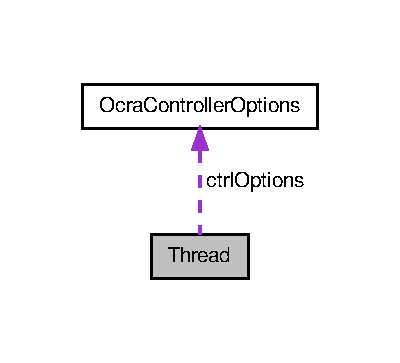
\includegraphics[width=192pt]{classThread__coll__graph}
\end{center}
\end{figure}
\subsection*{\-Classes}
\begin{DoxyCompactItemize}
\item 
class \hyperlink{classThread_1_1ControllerRpcServerCallback}{\-Controller\-Rpc\-Server\-Callback}
\begin{DoxyCompactList}\small\item\em \-A callback function which binds the rpc server port opened in the contoller server module to the controller thread's parsing function. \end{DoxyCompactList}\item 
class \hyperlink{classThread_1_1DebugRpcServerCallback}{\-Debug\-Rpc\-Server\-Callback}
\begin{DoxyCompactList}\small\item\em \-A callback function which binds the rpc server port opened in the contoller server module to the controller thread's parsing function. \end{DoxyCompactList}\end{DoxyCompactItemize}
\subsection*{\-Public \-Member \-Functions}
\begin{DoxyCompactItemize}
\item 
\hyperlink{classThread_a7494a3cf676527432ee724d59ed9ee8f}{\-Thread} (\hyperlink{classOcraControllerOptions}{\-Ocra\-Controller\-Options} \&controller\-\_\-options, std\-::shared\-\_\-ptr$<$ wbi\-::whole\-Body\-Interface $>$ wbi)
\item 
virtual \hyperlink{classThread_a37d9edd3a1a776cbc27dedff949c9726}{$\sim$\-Thread} ()
\item 
bool \hyperlink{classThread_a1e840470cd71d7bfb2430d24169e3dce}{thread\-Init} ()
\item 
void \hyperlink{classThread_ad9373d8d725c46717dfce3130018fe3a}{run} ()
\item 
void \hyperlink{classThread_aa2856c7d45670f45d66bcb319255defe}{thread\-Release} ()
\end{DoxyCompactItemize}
\subsection*{\-Private \-Member \-Functions}
\begin{DoxyCompactItemize}
\item 
\hyperlink{namespaceocra__icub_afbd2db66b68005fb7cfac19210caf83f}{ocra\-\_\-icub\-::\-O\-C\-R\-A\-\_\-\-I\-C\-U\-B\-\_\-\-M\-E\-S\-S\-A\-G\-E} \hyperlink{classThread_a2c64d83df66f7168d34993b76a179dde}{convert\-String\-To\-Ocra\-Icub\-Message} (const std\-::string \&s)
\item 
void \hyperlink{classThread_ae21029d250ac7c720f2411eab71a9414}{parse\-Incoming\-Message} (yarp\-::os\-::\-Bottle \&input, yarp\-::os\-::\-Bottle \&reply)
\item 
void \hyperlink{classThread_a6ce5ef9684cb2793be85e7402ad672f0}{parse\-Debug\-Message} (yarp\-::os\-::\-Bottle \&input, yarp\-::os\-::\-Bottle \&reply)
\item 
void \hyperlink{classThread_a9af0e98aa9b1de2f5c7bfa2f6e5001a2}{write\-Debug\-Data} ()
\item 
void \hyperlink{classThread_a49b65da88eb521ff53ef94d6ec8da7ab}{put\-Ankles\-Into\-Idle} ()
\end{DoxyCompactItemize}
\subsection*{\-Private \-Attributes}
\begin{DoxyCompactItemize}
\item 
ocra\-::\-Model\-::\-Ptr \hyperlink{classThread_a1dcef9aedc1a707e6f04d5fb6e4a0b13}{model}
\item 
std\-::shared\-\_\-ptr\*
$<$ \hyperlink{classIcubControllerServer}{\-Icub\-Controller\-Server} $>$ \hyperlink{classThread_ace1179249de64e545f43dc48529fbbb6}{ctrl\-Server}
\item 
\-Eigen\-::\-Array\-Xd \hyperlink{classThread_a414015415c64371877d6028417c4f9e2}{min\-Torques}
\item 
\-Eigen\-::\-Array\-Xd \hyperlink{classThread_af28a4fcbbcbf77c42237c0be75a25a54}{max\-Torques}
\item 
\hyperlink{classOcraControllerOptions}{\-Ocra\-Controller\-Options} \hyperlink{classThread_af96a166364f0c6a680115600b3bd232e}{ctrl\-Options}
\item 
std\-::shared\-\_\-ptr\*
$<$ wbi\-::whole\-Body\-Interface $>$ \hyperlink{classThread_aa3f4bbc2dca15c247a13de1bdbc4f7a3}{yarp\-Wbi}
\item 
\-Eigen\-::\-Vector\-Xd \hyperlink{classThread_a3238993799b36af06f3858a3f65dcf1e}{torques}
\item 
\-Eigen\-::\-Vector\-Xd \hyperlink{classThread_aa59863bb50c8aa88fe5872e75be44cb7}{initial\-Posture}
\item 
\hyperlink{namespaceocra__icub_afbd2db66b68005fb7cfac19210caf83f}{ocra\-\_\-icub\-::\-O\-C\-R\-A\-\_\-\-I\-C\-U\-B\-\_\-\-M\-E\-S\-S\-A\-G\-E} \hyperlink{classThread_a913cf23e86cdaefd036b782f7417254d}{controller\-Status}
\item 
\-Controller\-Rpc\-Server\-Callback\-::shared\-\_\-ptr \hyperlink{classThread_a602de8d12886c9c57b5420c83804a38b}{rpc\-Server\-Callback}
\item 
yarp\-::os\-::\-Rpc\-Server \hyperlink{classThread_adbec1b4f2c8fc40641df6f118e93fd25}{rpc\-Server\-Port}
\item 
int \hyperlink{classThread_aedf960b8e991868561f35193702245b0}{debug\-Joint\-Index}
\item 
yarp\-::os\-::\-Rpc\-Server \hyperlink{classThread_aa6b8f3712e7776d560b0a535eff73c34}{debug\-Rpc\-Port}
\item 
yarp\-::os\-::\-Port \hyperlink{classThread_a3780b51f82c50fd2738afbd0ae9b9526}{debug\-Ref\-Out\-Port}
\item 
yarp\-::os\-::\-Port \hyperlink{classThread_a9bd7f6aebc0be4709f32f95aa32f1add}{debug\-Real\-Out\-Port}
\item 
\-Debug\-Rpc\-Server\-Callback\-::shared\-\_\-ptr \hyperlink{classThread_a42833af67d5280e6946a31a03737e017}{debug\-Rpc\-Callback}
\item 
\-Eigen\-::\-Vector\-Xd \hyperlink{classThread_aa9cbe8744e51571a17fa726d8d16a0c6}{measured\-Torques}
\item 
bool \hyperlink{classThread_aba345996b91a57d9e1f2dd15c7c75e08}{debugging\-All\-Joints}
\item 
\-Eigen\-::\-Displacementd \hyperlink{classThread_a304e7ee40ec0ceec2fc7ca80353ab478}{l\-\_\-foot\-\_\-disp\-\_\-inverse}
\item 
i\-Dyn\-Tree\-::\-Simple\-Legged\-Odometry \hyperlink{classThread_a23a41c6ccd1df898084112cfd46120f3}{odometry}
\end{DoxyCompactItemize}
\subsection*{\-Static \-Private \-Attributes}
\begin{DoxyCompactItemize}
\item 
static const int \hyperlink{classThread_a875b3311a39e3b87dbc981f2db7b1b9d}{\-A\-L\-L\-\_\-\-J\-O\-I\-N\-T\-S} = -\/1
\item 
static const int \hyperlink{classThread_ad44e5fbda8070c252ea71823a4b9a6db}{\-T\-O\-R\-Q\-U\-E\-\_\-\-M\-I\-N} = -\/24
\item 
static const int \hyperlink{classThread_a5e864394c4bd0fbdf3cba7f6f825e17d}{\-T\-O\-R\-Q\-U\-E\-\_\-\-M\-A\-X} = 24
\end{DoxyCompactItemize}


\subsection{\-Detailed \-Description}
\-The meat and potatoes of the controller server. 

\begin{DoxyRefDesc}{\-Todo}
\item[\hyperlink{todo__todo000001}{\-Todo}]\-Remove task sequences. \-This class sets up an ocra\-::\-Model which is constructed from an \-Ocra\-Wbi\-Model and an ocra\-::\-Controller which can be specified as either a \-Wocra\-Controller, a \-Gocra\-Controller, or a \-Hocra\-Controller. \-The thread is looped at the period specified by the user (defaults to 10ms) and on each loop the \-Model is updated and the control torques are recalculated. $\ast$\-At the writing of this comment, task sequences are still in use and they too are initialized and updated here. \-They will be removed eventually.$\ast$ \end{DoxyRefDesc}


\subsection{\-Constructor \& \-Destructor \-Documentation}
\hypertarget{classThread_a7494a3cf676527432ee724d59ed9ee8f}{\index{\-Thread@{\-Thread}!\-Thread@{\-Thread}}
\index{\-Thread@{\-Thread}!Thread@{\-Thread}}
\subsubsection[{\-Thread}]{\setlength{\rightskip}{0pt plus 5cm}{\bf \-Thread\-::\-Thread} (
\begin{DoxyParamCaption}
\item[{{\bf \-Ocra\-Controller\-Options} \&}]{controller\-\_\-options, }
\item[{std\-::shared\-\_\-ptr$<$ wbi\-::whole\-Body\-Interface $>$}]{wbi}
\end{DoxyParamCaption}
)}}\label{classThread_a7494a3cf676527432ee724d59ed9ee8f}
\-Constructor 
\begin{DoxyParams}{\-Parameters}
{\em controller\-\_\-options} & \-The various arguments and options used to define what type of controller and tasks to use. \-See \hyperlink{classOcraControllerOptions}{\-Ocra\-Controller\-Options}. \\
\hline
{\em wbi} & \-A shared pointer to a whole\-Body\-Interface object. \\
\hline
\end{DoxyParams}
\hypertarget{classThread_a37d9edd3a1a776cbc27dedff949c9726}{\index{\-Thread@{\-Thread}!$\sim$\-Thread@{$\sim$\-Thread}}
\index{$\sim$\-Thread@{$\sim$\-Thread}!Thread@{\-Thread}}
\subsubsection[{$\sim$\-Thread}]{\setlength{\rightskip}{0pt plus 5cm}{\bf \-Thread\-::$\sim$\-Thread} (
\begin{DoxyParamCaption}
{}
\end{DoxyParamCaption}
)\hspace{0.3cm}{\ttfamily  \mbox{[}virtual\mbox{]}}}}\label{classThread_a37d9edd3a1a776cbc27dedff949c9726}


\subsection{\-Member \-Function \-Documentation}
\hypertarget{classThread_a2c64d83df66f7168d34993b76a179dde}{\index{\-Thread@{\-Thread}!convert\-String\-To\-Ocra\-Icub\-Message@{convert\-String\-To\-Ocra\-Icub\-Message}}
\index{convert\-String\-To\-Ocra\-Icub\-Message@{convert\-String\-To\-Ocra\-Icub\-Message}!Thread@{\-Thread}}
\subsubsection[{convert\-String\-To\-Ocra\-Icub\-Message}]{\setlength{\rightskip}{0pt plus 5cm}{\bf ocra\-\_\-icub\-::\-O\-C\-R\-A\-\_\-\-I\-C\-U\-B\-\_\-\-M\-E\-S\-S\-A\-G\-E} {\bf \-Thread\-::convert\-String\-To\-Ocra\-Icub\-Message} (
\begin{DoxyParamCaption}
\item[{const std\-::string \&}]{s}
\end{DoxyParamCaption}
)\hspace{0.3cm}{\ttfamily  \mbox{[}private\mbox{]}}}}\label{classThread_a2c64d83df66f7168d34993b76a179dde}
\hypertarget{classThread_a6ce5ef9684cb2793be85e7402ad672f0}{\index{\-Thread@{\-Thread}!parse\-Debug\-Message@{parse\-Debug\-Message}}
\index{parse\-Debug\-Message@{parse\-Debug\-Message}!Thread@{\-Thread}}
\subsubsection[{parse\-Debug\-Message}]{\setlength{\rightskip}{0pt plus 5cm}void {\bf \-Thread\-::parse\-Debug\-Message} (
\begin{DoxyParamCaption}
\item[{yarp\-::os\-::\-Bottle \&}]{input, }
\item[{yarp\-::os\-::\-Bottle \&}]{reply}
\end{DoxyParamCaption}
)\hspace{0.3cm}{\ttfamily  \mbox{[}private\mbox{]}}}}\label{classThread_a6ce5ef9684cb2793be85e7402ad672f0}
\hypertarget{classThread_ae21029d250ac7c720f2411eab71a9414}{\index{\-Thread@{\-Thread}!parse\-Incoming\-Message@{parse\-Incoming\-Message}}
\index{parse\-Incoming\-Message@{parse\-Incoming\-Message}!Thread@{\-Thread}}
\subsubsection[{parse\-Incoming\-Message}]{\setlength{\rightskip}{0pt plus 5cm}void {\bf \-Thread\-::parse\-Incoming\-Message} (
\begin{DoxyParamCaption}
\item[{yarp\-::os\-::\-Bottle \&}]{input, }
\item[{yarp\-::os\-::\-Bottle \&}]{reply}
\end{DoxyParamCaption}
)\hspace{0.3cm}{\ttfamily  \mbox{[}private\mbox{]}}}}\label{classThread_ae21029d250ac7c720f2411eab71a9414}
\hypertarget{classThread_a49b65da88eb521ff53ef94d6ec8da7ab}{\index{\-Thread@{\-Thread}!put\-Ankles\-Into\-Idle@{put\-Ankles\-Into\-Idle}}
\index{put\-Ankles\-Into\-Idle@{put\-Ankles\-Into\-Idle}!Thread@{\-Thread}}
\subsubsection[{put\-Ankles\-Into\-Idle}]{\setlength{\rightskip}{0pt plus 5cm}void {\bf \-Thread\-::put\-Ankles\-Into\-Idle} (
\begin{DoxyParamCaption}
{}
\end{DoxyParamCaption}
)\hspace{0.3cm}{\ttfamily  \mbox{[}private\mbox{]}}}}\label{classThread_a49b65da88eb521ff53ef94d6ec8da7ab}
\hypertarget{classThread_ad9373d8d725c46717dfce3130018fe3a}{\index{\-Thread@{\-Thread}!run@{run}}
\index{run@{run}!Thread@{\-Thread}}
\subsubsection[{run}]{\setlength{\rightskip}{0pt plus 5cm}void {\bf \-Thread\-::run} (
\begin{DoxyParamCaption}
{}
\end{DoxyParamCaption}
)}}\label{classThread_ad9373d8d725c46717dfce3130018fe3a}
\hypertarget{classThread_a1e840470cd71d7bfb2430d24169e3dce}{\index{\-Thread@{\-Thread}!thread\-Init@{thread\-Init}}
\index{thread\-Init@{thread\-Init}!Thread@{\-Thread}}
\subsubsection[{thread\-Init}]{\setlength{\rightskip}{0pt plus 5cm}bool {\bf \-Thread\-::thread\-Init} (
\begin{DoxyParamCaption}
{}
\end{DoxyParamCaption}
)}}\label{classThread_a1e840470cd71d7bfb2430d24169e3dce}
\hypertarget{classThread_aa2856c7d45670f45d66bcb319255defe}{\index{\-Thread@{\-Thread}!thread\-Release@{thread\-Release}}
\index{thread\-Release@{thread\-Release}!Thread@{\-Thread}}
\subsubsection[{thread\-Release}]{\setlength{\rightskip}{0pt plus 5cm}void {\bf \-Thread\-::thread\-Release} (
\begin{DoxyParamCaption}
{}
\end{DoxyParamCaption}
)}}\label{classThread_aa2856c7d45670f45d66bcb319255defe}
\hypertarget{classThread_a9af0e98aa9b1de2f5c7bfa2f6e5001a2}{\index{\-Thread@{\-Thread}!write\-Debug\-Data@{write\-Debug\-Data}}
\index{write\-Debug\-Data@{write\-Debug\-Data}!Thread@{\-Thread}}
\subsubsection[{write\-Debug\-Data}]{\setlength{\rightskip}{0pt plus 5cm}void {\bf \-Thread\-::write\-Debug\-Data} (
\begin{DoxyParamCaption}
{}
\end{DoxyParamCaption}
)\hspace{0.3cm}{\ttfamily  \mbox{[}private\mbox{]}}}}\label{classThread_a9af0e98aa9b1de2f5c7bfa2f6e5001a2}


\subsection{\-Member \-Data \-Documentation}
\hypertarget{classThread_a875b3311a39e3b87dbc981f2db7b1b9d}{\index{\-Thread@{\-Thread}!\-A\-L\-L\-\_\-\-J\-O\-I\-N\-T\-S@{\-A\-L\-L\-\_\-\-J\-O\-I\-N\-T\-S}}
\index{\-A\-L\-L\-\_\-\-J\-O\-I\-N\-T\-S@{\-A\-L\-L\-\_\-\-J\-O\-I\-N\-T\-S}!Thread@{\-Thread}}
\subsubsection[{\-A\-L\-L\-\_\-\-J\-O\-I\-N\-T\-S}]{\setlength{\rightskip}{0pt plus 5cm}const int {\bf \-Thread\-::\-A\-L\-L\-\_\-\-J\-O\-I\-N\-T\-S} = -\/1\hspace{0.3cm}{\ttfamily  \mbox{[}static, private\mbox{]}}}}\label{classThread_a875b3311a39e3b87dbc981f2db7b1b9d}
\-Maximum possible actuator torques \hypertarget{classThread_a913cf23e86cdaefd036b782f7417254d}{\index{\-Thread@{\-Thread}!controller\-Status@{controller\-Status}}
\index{controller\-Status@{controller\-Status}!Thread@{\-Thread}}
\subsubsection[{controller\-Status}]{\setlength{\rightskip}{0pt plus 5cm}{\bf ocra\-\_\-icub\-::\-O\-C\-R\-A\-\_\-\-I\-C\-U\-B\-\_\-\-M\-E\-S\-S\-A\-G\-E} {\bf \-Thread\-::controller\-Status}\hspace{0.3cm}{\ttfamily  \mbox{[}private\mbox{]}}}}\label{classThread_a913cf23e86cdaefd036b782f7417254d}
\hypertarget{classThread_af96a166364f0c6a680115600b3bd232e}{\index{\-Thread@{\-Thread}!ctrl\-Options@{ctrl\-Options}}
\index{ctrl\-Options@{ctrl\-Options}!Thread@{\-Thread}}
\subsubsection[{ctrl\-Options}]{\setlength{\rightskip}{0pt plus 5cm}{\bf \-Ocra\-Controller\-Options} {\bf \-Thread\-::ctrl\-Options}\hspace{0.3cm}{\ttfamily  \mbox{[}private\mbox{]}}}}\label{classThread_af96a166364f0c6a680115600b3bd232e}
\-The controller options. \hypertarget{classThread_ace1179249de64e545f43dc48529fbbb6}{\index{\-Thread@{\-Thread}!ctrl\-Server@{ctrl\-Server}}
\index{ctrl\-Server@{ctrl\-Server}!Thread@{\-Thread}}
\subsubsection[{ctrl\-Server}]{\setlength{\rightskip}{0pt plus 5cm}std\-::shared\-\_\-ptr$<${\bf \-Icub\-Controller\-Server}$>$ {\bf \-Thread\-::ctrl\-Server}\hspace{0.3cm}{\ttfamily  \mbox{[}private\mbox{]}}}}\label{classThread_ace1179249de64e545f43dc48529fbbb6}
\hypertarget{classThread_aba345996b91a57d9e1f2dd15c7c75e08}{\index{\-Thread@{\-Thread}!debugging\-All\-Joints@{debugging\-All\-Joints}}
\index{debugging\-All\-Joints@{debugging\-All\-Joints}!Thread@{\-Thread}}
\subsubsection[{debugging\-All\-Joints}]{\setlength{\rightskip}{0pt plus 5cm}bool {\bf \-Thread\-::debugging\-All\-Joints}\hspace{0.3cm}{\ttfamily  \mbox{[}private\mbox{]}}}}\label{classThread_aba345996b91a57d9e1f2dd15c7c75e08}
\hypertarget{classThread_aedf960b8e991868561f35193702245b0}{\index{\-Thread@{\-Thread}!debug\-Joint\-Index@{debug\-Joint\-Index}}
\index{debug\-Joint\-Index@{debug\-Joint\-Index}!Thread@{\-Thread}}
\subsubsection[{debug\-Joint\-Index}]{\setlength{\rightskip}{0pt plus 5cm}int {\bf \-Thread\-::debug\-Joint\-Index}\hspace{0.3cm}{\ttfamily  \mbox{[}private\mbox{]}}}}\label{classThread_aedf960b8e991868561f35193702245b0}
\hypertarget{classThread_a9bd7f6aebc0be4709f32f95aa32f1add}{\index{\-Thread@{\-Thread}!debug\-Real\-Out\-Port@{debug\-Real\-Out\-Port}}
\index{debug\-Real\-Out\-Port@{debug\-Real\-Out\-Port}!Thread@{\-Thread}}
\subsubsection[{debug\-Real\-Out\-Port}]{\setlength{\rightskip}{0pt plus 5cm}yarp\-::os\-::\-Port {\bf \-Thread\-::debug\-Real\-Out\-Port}\hspace{0.3cm}{\ttfamily  \mbox{[}private\mbox{]}}}}\label{classThread_a9bd7f6aebc0be4709f32f95aa32f1add}
\hypertarget{classThread_a3780b51f82c50fd2738afbd0ae9b9526}{\index{\-Thread@{\-Thread}!debug\-Ref\-Out\-Port@{debug\-Ref\-Out\-Port}}
\index{debug\-Ref\-Out\-Port@{debug\-Ref\-Out\-Port}!Thread@{\-Thread}}
\subsubsection[{debug\-Ref\-Out\-Port}]{\setlength{\rightskip}{0pt plus 5cm}yarp\-::os\-::\-Port {\bf \-Thread\-::debug\-Ref\-Out\-Port}\hspace{0.3cm}{\ttfamily  \mbox{[}private\mbox{]}}}}\label{classThread_a3780b51f82c50fd2738afbd0ae9b9526}
\hypertarget{classThread_a42833af67d5280e6946a31a03737e017}{\index{\-Thread@{\-Thread}!debug\-Rpc\-Callback@{debug\-Rpc\-Callback}}
\index{debug\-Rpc\-Callback@{debug\-Rpc\-Callback}!Thread@{\-Thread}}
\subsubsection[{debug\-Rpc\-Callback}]{\setlength{\rightskip}{0pt plus 5cm}\-Debug\-Rpc\-Server\-Callback\-::shared\-\_\-ptr {\bf \-Thread\-::debug\-Rpc\-Callback}\hspace{0.3cm}{\ttfamily  \mbox{[}private\mbox{]}}}}\label{classThread_a42833af67d5280e6946a31a03737e017}
\-Rpc server port callback function. \hypertarget{classThread_aa6b8f3712e7776d560b0a535eff73c34}{\index{\-Thread@{\-Thread}!debug\-Rpc\-Port@{debug\-Rpc\-Port}}
\index{debug\-Rpc\-Port@{debug\-Rpc\-Port}!Thread@{\-Thread}}
\subsubsection[{debug\-Rpc\-Port}]{\setlength{\rightskip}{0pt plus 5cm}yarp\-::os\-::\-Rpc\-Server {\bf \-Thread\-::debug\-Rpc\-Port}\hspace{0.3cm}{\ttfamily  \mbox{[}private\mbox{]}}}}\label{classThread_aa6b8f3712e7776d560b0a535eff73c34}
\hypertarget{classThread_aa59863bb50c8aa88fe5872e75be44cb7}{\index{\-Thread@{\-Thread}!initial\-Posture@{initial\-Posture}}
\index{initial\-Posture@{initial\-Posture}!Thread@{\-Thread}}
\subsubsection[{initial\-Posture}]{\setlength{\rightskip}{0pt plus 5cm}\-Eigen\-::\-Vector\-Xd {\bf \-Thread\-::initial\-Posture}\hspace{0.3cm}{\ttfamily  \mbox{[}private\mbox{]}}}}\label{classThread_aa59863bb50c8aa88fe5872e75be44cb7}
\-The torques calculated at each \hyperlink{classThread_ad9373d8d725c46717dfce3130018fe3a}{run()} loop. \hypertarget{classThread_a304e7ee40ec0ceec2fc7ca80353ab478}{\index{\-Thread@{\-Thread}!l\-\_\-foot\-\_\-disp\-\_\-inverse@{l\-\_\-foot\-\_\-disp\-\_\-inverse}}
\index{l\-\_\-foot\-\_\-disp\-\_\-inverse@{l\-\_\-foot\-\_\-disp\-\_\-inverse}!Thread@{\-Thread}}
\subsubsection[{l\-\_\-foot\-\_\-disp\-\_\-inverse}]{\setlength{\rightskip}{0pt plus 5cm}\-Eigen\-::\-Displacementd {\bf \-Thread\-::l\-\_\-foot\-\_\-disp\-\_\-inverse}\hspace{0.3cm}{\ttfamily  \mbox{[}private\mbox{]}}}}\label{classThread_a304e7ee40ec0ceec2fc7ca80353ab478}
\-For gazebo visualization. \-You can't get the l\-\_\-sole pose directly in gazebo, but you can get the l\-\_\-foot, so since all poses from ocra\-::\-Model are calculated in the l\-\_\-sole then we need to go from l\-\_\-sole to l\-\_\-foot. \hypertarget{classThread_af28a4fcbbcbf77c42237c0be75a25a54}{\index{\-Thread@{\-Thread}!max\-Torques@{max\-Torques}}
\index{max\-Torques@{max\-Torques}!Thread@{\-Thread}}
\subsubsection[{max\-Torques}]{\setlength{\rightskip}{0pt plus 5cm}\-Eigen\-::\-Array\-Xd {\bf \-Thread\-::max\-Torques}\hspace{0.3cm}{\ttfamily  \mbox{[}private\mbox{]}}}}\label{classThread_af28a4fcbbcbf77c42237c0be75a25a54}
\-An eigen array filled with the max torques. \hypertarget{classThread_aa9cbe8744e51571a17fa726d8d16a0c6}{\index{\-Thread@{\-Thread}!measured\-Torques@{measured\-Torques}}
\index{measured\-Torques@{measured\-Torques}!Thread@{\-Thread}}
\subsubsection[{measured\-Torques}]{\setlength{\rightskip}{0pt plus 5cm}\-Eigen\-::\-Vector\-Xd {\bf \-Thread\-::measured\-Torques}\hspace{0.3cm}{\ttfamily  \mbox{[}private\mbox{]}}}}\label{classThread_aa9cbe8744e51571a17fa726d8d16a0c6}
\hypertarget{classThread_a414015415c64371877d6028417c4f9e2}{\index{\-Thread@{\-Thread}!min\-Torques@{min\-Torques}}
\index{min\-Torques@{min\-Torques}!Thread@{\-Thread}}
\subsubsection[{min\-Torques}]{\setlength{\rightskip}{0pt plus 5cm}\-Eigen\-::\-Array\-Xd {\bf \-Thread\-::min\-Torques}\hspace{0.3cm}{\ttfamily  \mbox{[}private\mbox{]}}}}\label{classThread_a414015415c64371877d6028417c4f9e2}
\-An eigen array filled with the min torques. \hypertarget{classThread_a1dcef9aedc1a707e6f04d5fb6e4a0b13}{\index{\-Thread@{\-Thread}!model@{model}}
\index{model@{model}!Thread@{\-Thread}}
\subsubsection[{model}]{\setlength{\rightskip}{0pt plus 5cm}ocra\-::\-Model\-::\-Ptr {\bf \-Thread\-::model}\hspace{0.3cm}{\ttfamily  \mbox{[}private\mbox{]}}}}\label{classThread_a1dcef9aedc1a707e6f04d5fb6e4a0b13}
\hypertarget{classThread_a23a41c6ccd1df898084112cfd46120f3}{\index{\-Thread@{\-Thread}!odometry@{odometry}}
\index{odometry@{odometry}!Thread@{\-Thread}}
\subsubsection[{odometry}]{\setlength{\rightskip}{0pt plus 5cm}i\-Dyn\-Tree\-::\-Simple\-Legged\-Odometry {\bf \-Thread\-::odometry}\hspace{0.3cm}{\ttfamily  \mbox{[}private\mbox{]}}}}\label{classThread_a23a41c6ccd1df898084112cfd46120f3}
\-Odometry object \hypertarget{classThread_a602de8d12886c9c57b5420c83804a38b}{\index{\-Thread@{\-Thread}!rpc\-Server\-Callback@{rpc\-Server\-Callback}}
\index{rpc\-Server\-Callback@{rpc\-Server\-Callback}!Thread@{\-Thread}}
\subsubsection[{rpc\-Server\-Callback}]{\setlength{\rightskip}{0pt plus 5cm}\-Controller\-Rpc\-Server\-Callback\-::shared\-\_\-ptr {\bf \-Thread\-::rpc\-Server\-Callback}\hspace{0.3cm}{\ttfamily  \mbox{[}private\mbox{]}}}}\label{classThread_a602de8d12886c9c57b5420c83804a38b}
\-Rpc server port callback function. \hypertarget{classThread_adbec1b4f2c8fc40641df6f118e93fd25}{\index{\-Thread@{\-Thread}!rpc\-Server\-Port@{rpc\-Server\-Port}}
\index{rpc\-Server\-Port@{rpc\-Server\-Port}!Thread@{\-Thread}}
\subsubsection[{rpc\-Server\-Port}]{\setlength{\rightskip}{0pt plus 5cm}yarp\-::os\-::\-Rpc\-Server {\bf \-Thread\-::rpc\-Server\-Port}\hspace{0.3cm}{\ttfamily  \mbox{[}private\mbox{]}}}}\label{classThread_adbec1b4f2c8fc40641df6f118e93fd25}
\-Rpc server port. \hypertarget{classThread_a5e864394c4bd0fbdf3cba7f6f825e17d}{\index{\-Thread@{\-Thread}!\-T\-O\-R\-Q\-U\-E\-\_\-\-M\-A\-X@{\-T\-O\-R\-Q\-U\-E\-\_\-\-M\-A\-X}}
\index{\-T\-O\-R\-Q\-U\-E\-\_\-\-M\-A\-X@{\-T\-O\-R\-Q\-U\-E\-\_\-\-M\-A\-X}!Thread@{\-Thread}}
\subsubsection[{\-T\-O\-R\-Q\-U\-E\-\_\-\-M\-A\-X}]{\setlength{\rightskip}{0pt plus 5cm}const int {\bf \-Thread\-::\-T\-O\-R\-Q\-U\-E\-\_\-\-M\-A\-X} = 24\hspace{0.3cm}{\ttfamily  \mbox{[}static, private\mbox{]}}}}\label{classThread_a5e864394c4bd0fbdf3cba7f6f825e17d}
\-Maximum possible actuator torques \hypertarget{classThread_ad44e5fbda8070c252ea71823a4b9a6db}{\index{\-Thread@{\-Thread}!\-T\-O\-R\-Q\-U\-E\-\_\-\-M\-I\-N@{\-T\-O\-R\-Q\-U\-E\-\_\-\-M\-I\-N}}
\index{\-T\-O\-R\-Q\-U\-E\-\_\-\-M\-I\-N@{\-T\-O\-R\-Q\-U\-E\-\_\-\-M\-I\-N}!Thread@{\-Thread}}
\subsubsection[{\-T\-O\-R\-Q\-U\-E\-\_\-\-M\-I\-N}]{\setlength{\rightskip}{0pt plus 5cm}const int {\bf \-Thread\-::\-T\-O\-R\-Q\-U\-E\-\_\-\-M\-I\-N} = -\/24\hspace{0.3cm}{\ttfamily  \mbox{[}static, private\mbox{]}}}}\label{classThread_ad44e5fbda8070c252ea71823a4b9a6db}
\-Minimum possible actuator torques \hypertarget{classThread_a3238993799b36af06f3858a3f65dcf1e}{\index{\-Thread@{\-Thread}!torques@{torques}}
\index{torques@{torques}!Thread@{\-Thread}}
\subsubsection[{torques}]{\setlength{\rightskip}{0pt plus 5cm}\-Eigen\-::\-Vector\-Xd {\bf \-Thread\-::torques}\hspace{0.3cm}{\ttfamily  \mbox{[}private\mbox{]}}}}\label{classThread_a3238993799b36af06f3858a3f65dcf1e}
\-The torques calculated at each \hyperlink{classThread_ad9373d8d725c46717dfce3130018fe3a}{run()} loop. \hypertarget{classThread_aa3f4bbc2dca15c247a13de1bdbc4f7a3}{\index{\-Thread@{\-Thread}!yarp\-Wbi@{yarp\-Wbi}}
\index{yarp\-Wbi@{yarp\-Wbi}!Thread@{\-Thread}}
\subsubsection[{yarp\-Wbi}]{\setlength{\rightskip}{0pt plus 5cm}std\-::shared\-\_\-ptr$<$wbi\-::whole\-Body\-Interface$>$ {\bf \-Thread\-::yarp\-Wbi}\hspace{0.3cm}{\ttfamily  \mbox{[}private\mbox{]}}}}\label{classThread_aa3f4bbc2dca15c247a13de1bdbc4f7a3}
\-The \-W\-B\-I used to talk to the robot. 

\-The documentation for this class was generated from the following files\-:\begin{DoxyCompactItemize}
\item 
ocra-\/wbi-\/plugins/ocra-\/icub-\/server/include/ocra-\/icub-\/server/\hyperlink{Thread_8h}{\-Thread.\-h}\item 
ocra-\/wbi-\/plugins/ocra-\/icub-\/server/src/\hyperlink{Thread_8cpp}{\-Thread.\-cpp}\end{DoxyCompactItemize}

\hypertarget{classWalkingClient}{\section{\-Walking\-Client \-Class \-Reference}
\label{classWalkingClient}\index{\-Walking\-Client@{\-Walking\-Client}}
}


{\ttfamily \#include $<$\-Walking\-Client.\-h$>$}

\subsection*{\-Public \-Member \-Functions}
\begin{DoxyCompactItemize}
\item 
\hyperlink{classWalkingClient_a6c9002a44a54814c4b482739824e39aa}{\-Walking\-Client} (std\-::shared\-\_\-ptr$<$ ocra\-::\-Model $>$ model\-Ptr, const int loop\-Period)
\item 
virtual \hyperlink{classWalkingClient_a1dbc0308f844aea6542750104fddf8e2}{$\sim$\-Walking\-Client} ()
\item 
bool \hyperlink{classWalkingClient_adb8f972f34cb39c69c02a7c3cb493b81}{configure} (yarp\-::os\-::\-Resource\-Finder \&rf)
\item 
void \hyperlink{classWalkingClient_aff3fabef11d9c8b747a422f879c26067}{print\-Help} ()
\item 
bool \hyperlink{classWalkingClient_a03ea2313c954a97aeb4d5b614f3e6caa}{read\-Foot\-Wrench} (\hyperlink{ZmpController_8h_a4b6a8e135f90bd56e5a57a60efb42529}{\-F\-O\-O\-T} which\-Foot, \-Eigen\-::\-Vector\-Xd \&raw\-Wrench)
\item 
std\-::vector$<$ \-Eigen\-::\-Vector2d $>$ \hyperlink{classWalkingClient_a3185a8ede8bf8b1227f7dd540ba87e3c}{generate\-Z\-M\-P\-Trajectory\-T\-E\-S\-T} (const double t\-Trans, const double feet\-Separation, const double time\-Step, const int amplitude\-Fraction, const int \-N)
\item 
bool \hyperlink{classWalkingClient_a87e70046251149b4b7aff1dc57b3dcc4}{get\-Feet\-Separation} (\-Eigen\-::\-Vector3d \&sep)
\item 
bool \hyperlink{classWalkingClient_ae6d6c046a9a3e51771afe8b4c105b412}{publish3d\-Quantity} (yarp\-::os\-::\-Buffered\-Port$<$ yarp\-::os\-::\-Bottle $>$ \&port, \-Eigen\-::\-Vector3d \&value)
\item 
void \hyperlink{classWalkingClient_ae3c259f7615c85ce53a413f6e7ab4b76}{perform\-Z\-M\-P\-Test} (\hyperlink{WalkingClient_8h_afc01479a47f5a87462a54b6a9e11fffa}{\-Zmp\-Test\-Type} type)
\item 
void \hyperlink{classWalkingClient_a3b1217b7fa17f76f162be0e12e419d96}{perform\-Z\-M\-P\-Preview\-Test} (\hyperlink{WalkingClient_8h_afc01479a47f5a87462a54b6a9e11fffa}{\-Zmp\-Test\-Type} type)
\item 
std\-::string \hyperlink{classWalkingClient_ae8f7dc629313df7d362e3edd6f45ae10}{compose\-Port\-Name} (std\-::string port\-Name)
\item 
void \hyperlink{classWalkingClient_ab4148804702e065310a903112bc10162}{transform\-Std\-Vector\-To\-Eigen\-Vector} (std\-::vector$<$ \-Eigen\-::\-Vector2d $>$ \&full\-Traj, int from, int \-Nc, \-Vector\-Xd \&output)
\item 
std\-::vector$<$ \-Eigen\-::\-Vector2d $>$ \hyperlink{classWalkingClient_a70b2375134ae55a041fbf30180ea3a8f}{generate\-Z\-M\-P\-Step\-Trajectory\-T\-E\-S\-T} (double feet\-Separation, double period, double duration, double rise\-Time, double constant\-Reference\-Y)
\item 
void \hyperlink{classWalkingClient_aad39a3836319f9b7258d8eb129776b47}{prepare\-Andset\-Desired\-Co\-M\-Task\-State} (\-Eigen\-::\-Vector\-Xd com\-State, bool do\-Set)
\end{DoxyCompactItemize}
\subsection*{\-Public \-Attributes}
\begin{DoxyCompactItemize}
\item 
yarp\-::os\-::\-Buffered\-Port\*
$<$ yarp\-::sig\-::\-Vector $>$ \hyperlink{classWalkingClient_a88ee63ff6a341eccd458d24700383457}{port\-Wrench\-Left\-Foot}
\item 
yarp\-::os\-::\-Buffered\-Port\*
$<$ yarp\-::sig\-::\-Vector $>$ \hyperlink{classWalkingClient_a96321dc60e84c193f2dea6e85983ca67}{port\-Wrench\-Right\-Foot}
\end{DoxyCompactItemize}
\subsection*{\-Protected \-Member \-Functions}
\begin{DoxyCompactItemize}
\item 
virtual bool \hyperlink{classWalkingClient_aba6a03fe29a4e947bc6bc0c09a713b2a}{initialize} ()
\item 
virtual void \hyperlink{classWalkingClient_a3b36da9d7649865a13c9318dd73ebc7e}{release} ()
\item 
virtual void \hyperlink{classWalkingClient_afd997bb00534c57fe1b0d5f37f207386}{loop} ()
\end{DoxyCompactItemize}
\subsection*{\-Private \-Attributes}
\begin{DoxyCompactItemize}
\item 
std\-::shared\-\_\-ptr$<$ \hyperlink{structZmpPreviewParams}{\-Zmp\-Preview\-Params} $>$ \hyperlink{classWalkingClient_a9a2cf2d6107ab91fc5bd1d82a3b85a84}{\-\_\-zmp\-Preview\-Params}
\item 
std\-::shared\-\_\-ptr\*
$<$ \hyperlink{classZmpPreviewController}{\-Zmp\-Preview\-Controller} $>$ \hyperlink{classWalkingClient_ae570aa07bed9e336eda93f331f3485fb}{\-\_\-zmp\-Preview\-Controller}
\item 
std\-::shared\-\_\-ptr\*
$<$ ocra\-\_\-recipes\-::\-Task\-Connection $>$ \hyperlink{classWalkingClient_aa798d6193535e80816f8107ee5fb2172}{\-\_\-com\-Task}
\item 
std\-::vector$<$ \-Eigen\-::\-Vector2d $>$ \hyperlink{classWalkingClient_a8b8a3d7fe6e12d49a0e72d05f9938564}{\-\_\-zmp\-Trajectory}
\item 
ocra\-::\-Task\-State \hyperlink{classWalkingClient_a2625bf687aa3141f5a2404c8d9b3c392}{\-\_\-desired\-Com\-State}
\item 
\-Eigen\-::\-Vector\-Xd \hyperlink{classWalkingClient_a1c3fb4d182e33d6d9386e9bb05aa4ae8}{\-\_\-raw\-Left\-Foot\-Wrench}
\item 
\-Eigen\-::\-Vector\-Xd \hyperlink{classWalkingClient_a9df32e0c73632c5f869e5933e20def71}{\-\_\-raw\-Right\-Foot\-Wrench}
\item 
\-Eigen\-::\-Vector2d \hyperlink{classWalkingClient_aa784eac1247f0d858e2364e0c2bc25b2}{\-\_\-global\-Z\-M\-P}
\item 
\-Eigen\-::\-Vector2d \hyperlink{classWalkingClient_a549751e511e023d5fc73eccd1c185317}{\-\_\-previous\-C\-O\-M}
\item 
\-Eigen\-::\-Vector2d \hyperlink{classWalkingClient_aa0c7669193a8a42ed289c79523580033}{\-\_\-previous\-C\-O\-M\-Vel}
\item 
std\-::string \hyperlink{classWalkingClient_aff02b341d5e1f500dc9a849337319a8d}{\-\_\-client\-Name}
\item 
std\-::string \hyperlink{classWalkingClient_a67461634d7e8cb0234400b34fd2865e7}{\-\_\-robot}
\item 
bool \hyperlink{classWalkingClient_a4f9c8688537ddd8a487a212fbb279a9b}{\-\_\-is\-Test\-Run}
\item 
std\-::string \hyperlink{classWalkingClient_a35c00feb4e7dfa532e43241e855fec89}{\-\_\-test\-Type}
\item 
\hyperlink{WalkingClient_8h_afc01479a47f5a87462a54b6a9e11fffa}{\-Zmp\-Test\-Type} \hyperlink{classWalkingClient_a14576258d7fed1b36919145f1b56d74c}{\-\_\-zmp\-Test\-Type}
\item 
std\-::string \hyperlink{classWalkingClient_ade3bf018661152fc0404d3973ea30783}{\-\_\-home\-Data\-Dir}
\item 
double \hyperlink{classWalkingClient_a4e448bc147b41d97e0f17af6ebb0020f}{\-\_\-com\-Y\-Const\-Vel}
\item 
double \hyperlink{classWalkingClient_a9f19b1a1184cbdbf883cc374c6b6b88f}{\-\_\-stop\-Time\-Const\-Com\-Vel}
\item 
double \hyperlink{classWalkingClient_a6cba3194816a0be78a8b17d539806115}{\-\_\-zmp\-Y\-Const\-Ref}
\item 
double \hyperlink{classWalkingClient_a58b08317f6d8b825a21e1db8c7f0ff32}{\-\_\-stop\-Time\-Const\-Zmp}
\item 
double \hyperlink{classWalkingClient_a144518766ec4eb9eeab230fcb291e20c}{\-\_\-t\-Trans}
\item 
int \hyperlink{classWalkingClient_aefb4ed994a32879a526f2bc8c962927f}{\-\_\-number\-Of\-Transitions}
\item 
int \hyperlink{classWalkingClient_ac548ce03ea9ceffb4b42981942f66dd0}{\-\_\-amplitude\-Fraction}
\item 
double \hyperlink{classWalkingClient_a2ed3837afa0c366f1cdef16b2a99b761}{\-\_\-stop\-Time\-Varying\-Zmp}
\item 
yarp\-::os\-::\-Buffered\-Port\*
$<$ yarp\-::os\-::\-Bottle $>$ \hyperlink{classWalkingClient_af2e0817fa94ca802775addd22b09bf7a}{\-\_\-zmp\-Port}
\item 
yarp\-::os\-::\-Buffered\-Port\*
$<$ yarp\-::os\-::\-Bottle $>$ \hyperlink{classWalkingClient_a1b01264c9d9d403a68a149d86d1bc53f}{\-\_\-dcom\-Error\-Port}
\item 
yarp\-::os\-::\-Buffered\-Port\*
$<$ yarp\-::os\-::\-Bottle $>$ \hyperlink{classWalkingClient_a17369473b4fe2ff0eaecc7d41a8430c7}{\-\_\-d\-Com\-Des\-Port}
\item 
yarp\-::os\-::\-Buffered\-Port\*
$<$ yarp\-::os\-::\-Bottle $>$ \hyperlink{classWalkingClient_a1fbc9d7f1e967f24acda745028f865df}{\-\_\-d\-Com\-Cur\-Port}
\item 
yarp\-::os\-::\-Buffered\-Port\*
$<$ yarp\-::os\-::\-Bottle $>$ \hyperlink{classWalkingClient_acbac3e142471448b50dd605e4217b0d0}{\-\_\-zmp\-Des\-Port}
\item 
yarp\-::os\-::\-Buffered\-Port\*
$<$ yarp\-::os\-::\-Bottle $>$ \hyperlink{classWalkingClient_a546e6830e43d19ba7d8a8e808e28ef53}{\-\_\-zmp\-Cur\-Port}
\item 
yarp\-::os\-::\-Buffered\-Port\*
$<$ yarp\-::os\-::\-Bottle $>$ \hyperlink{classWalkingClient_a199a104e0d4d52deae07d88d8229b60d}{\-\_\-com\-Current}
\item 
yarp\-::os\-::\-Buffered\-Port\*
$<$ yarp\-::os\-::\-Bottle $>$ \hyperlink{classWalkingClient_a692d95b3e76a396d107b0c29a3d591f1}{\-\_\-ddcom\-Current}
\item 
yarp\-::os\-::\-Buffered\-Port\*
$<$ yarp\-::os\-::\-Bottle $>$ \hyperlink{classWalkingClient_a41b7320607812418af496b8b2c30204f}{\-\_\-ddcom\-From\-Z\-M\-P}
\item 
\-Vector\-Xd \hyperlink{classWalkingClient_abc3c504305c00a27e9fd38a8bf08ecda}{\-\_\-hkk\-Previous}
\item 
bool \hyperlink{classWalkingClient_ab645ecb2d55e28b57a64ca48ee638b1e}{\-\_\-first\-Loop}
\item 
\-Eigen\-::\-Vector\-Xd \hyperlink{classWalkingClient_af28b3cd3b1202f83e193b098572fbdd3}{zmp\-Ref\-In\-Preview\-Window}
\item 
\-Eigen\-::\-Vector\-Xd \hyperlink{classWalkingClient_ab3b1defedb6d79b5b6eaadd52bbad9f5}{com\-Vel\-Ref\-In\-Preview\-Window}
\item 
\-Eigen\-::\-Vector\-Xd \hyperlink{classWalkingClient_a0e5aee88e377029d79f57e778c583f18}{optimal\-U}
\end{DoxyCompactItemize}


\subsection{\-Constructor \& \-Destructor \-Documentation}
\hypertarget{classWalkingClient_a6c9002a44a54814c4b482739824e39aa}{\index{\-Walking\-Client@{\-Walking\-Client}!\-Walking\-Client@{\-Walking\-Client}}
\index{\-Walking\-Client@{\-Walking\-Client}!WalkingClient@{\-Walking\-Client}}
\subsubsection[{\-Walking\-Client}]{\setlength{\rightskip}{0pt plus 5cm}{\bf \-Walking\-Client\-::\-Walking\-Client} (
\begin{DoxyParamCaption}
\item[{std\-::shared\-\_\-ptr$<$ ocra\-::\-Model $>$}]{model\-Ptr, }
\item[{const int}]{loop\-Period}
\end{DoxyParamCaption}
)}}\label{classWalkingClient_a6c9002a44a54814c4b482739824e39aa}
\hypertarget{classWalkingClient_a1dbc0308f844aea6542750104fddf8e2}{\index{\-Walking\-Client@{\-Walking\-Client}!$\sim$\-Walking\-Client@{$\sim$\-Walking\-Client}}
\index{$\sim$\-Walking\-Client@{$\sim$\-Walking\-Client}!WalkingClient@{\-Walking\-Client}}
\subsubsection[{$\sim$\-Walking\-Client}]{\setlength{\rightskip}{0pt plus 5cm}{\bf \-Walking\-Client\-::$\sim$\-Walking\-Client} (
\begin{DoxyParamCaption}
{}
\end{DoxyParamCaption}
)\hspace{0.3cm}{\ttfamily  \mbox{[}virtual\mbox{]}}}}\label{classWalkingClient_a1dbc0308f844aea6542750104fddf8e2}


\subsection{\-Member \-Function \-Documentation}
\hypertarget{classWalkingClient_ae8f7dc629313df7d362e3edd6f45ae10}{\index{\-Walking\-Client@{\-Walking\-Client}!compose\-Port\-Name@{compose\-Port\-Name}}
\index{compose\-Port\-Name@{compose\-Port\-Name}!WalkingClient@{\-Walking\-Client}}
\subsubsection[{compose\-Port\-Name}]{\setlength{\rightskip}{0pt plus 5cm}std\-::string {\bf \-Walking\-Client\-::compose\-Port\-Name} (
\begin{DoxyParamCaption}
\item[{std\-::string}]{port\-Name}
\end{DoxyParamCaption}
)}}\label{classWalkingClient_ae8f7dc629313df7d362e3edd6f45ae10}
\-Composes a port name with the client name as the suffix. \-This client name is assumed to be passed through command line options or configuration file as per the policies of yarp's \-Resource \-Finder.


\begin{DoxyParams}{\-Parameters}
{\em port\-Name} & \-Name of the port without backslashes. e.\-g. \char`\"{}zmp\-Error\-:o\char`\"{} \\
\hline
\end{DoxyParams}
\begin{DoxyReturn}{\-Returns}
\-A client-\/name-\/prepended port name, e.\-g. \char`\"{}/walking\-Client/zmp\-Error\-:o\char`\"{} 
\end{DoxyReturn}
\hypertarget{classWalkingClient_adb8f972f34cb39c69c02a7c3cb493b81}{\index{\-Walking\-Client@{\-Walking\-Client}!configure@{configure}}
\index{configure@{configure}!WalkingClient@{\-Walking\-Client}}
\subsubsection[{configure}]{\setlength{\rightskip}{0pt plus 5cm}bool {\bf \-Walking\-Client\-::configure} (
\begin{DoxyParamCaption}
\item[{yarp\-::os\-::\-Resource\-Finder \&}]{rf}
\end{DoxyParamCaption}
)}}\label{classWalkingClient_adb8f972f34cb39c69c02a7c3cb493b81}
\-Takes all the parameters used by this client from configuration file and parses them through yarp's \-Resource \-Finder.

\-Details on group \mbox{[}\-Z\-M\-P\-\_\-\-C\-O\-N\-T\-R\-O\-L\-L\-E\-R\-\_\-\-P\-A\-R\-A\-M\-S\mbox{]} in walking-\/client.\-ini \-Options are\-: 0 -\/ \-Z\-M\-P\-\_\-\-C\-O\-N\-S\-T\-A\-N\-T\-\_\-\-R\-E\-F\-E\-R\-E\-N\-C\-E 1 -\/ \-Z\-M\-P\-\_\-\-V\-A\-R\-Y\-I\-N\-G\-\_\-\-R\-E\-F\-E\-R\-E\-N\-C\-E 2 -\/ \-C\-O\-M\-\_\-\-L\-I\-N\-\_\-\-V\-E\-L\-\_\-\-C\-O\-N\-S\-T\-A\-N\-T\-\_\-\-R\-E\-F\-E\-R\-E\-N\-C\-E \-Each of these tests are used to evaluate the correct gains to be used at each level of the control loops. \-These trajectorie will be used during the tests specified through the option 'test' which takes the values \char`\"{}zmp\-Preview\char`\"{} or \char`\"{}zmp\-Controller\char`\"{}. \-When using this client for the first time on a robot, the gains of the com\-Task in its corresponding task\-Set file must be tuned first as well and later those for the \hyperlink{classZmpController}{\-Zmp\-Controller} class. \-Therefore we recommend executing this client first as a way of testing the \char`\"{}low\char`\"{} level \-Com\-Task control in order to find good kp and kd. \-Do this by setting 'type' to 2. \-Data will be saved at the location you specify through the option 'home\-Data\-Dir'. \-After having a good \-C\-O\-M velocity tracking at the task level, you want to test the tracking of the zmp controller by setting 'type' to 0. \-A constant zmp reference is given and the controller gains kfx, kfy, kdx and kdy must be tuned accordingly. \-Finally, the tracking of varying zmp reference can be tested which takes the zmp from left to right, while the robot stands on both feet. \hypertarget{classWalkingClient_a70b2375134ae55a041fbf30180ea3a8f}{\index{\-Walking\-Client@{\-Walking\-Client}!generate\-Z\-M\-P\-Step\-Trajectory\-T\-E\-S\-T@{generate\-Z\-M\-P\-Step\-Trajectory\-T\-E\-S\-T}}
\index{generate\-Z\-M\-P\-Step\-Trajectory\-T\-E\-S\-T@{generate\-Z\-M\-P\-Step\-Trajectory\-T\-E\-S\-T}!WalkingClient@{\-Walking\-Client}}
\subsubsection[{generate\-Z\-M\-P\-Step\-Trajectory\-T\-E\-S\-T}]{\setlength{\rightskip}{0pt plus 5cm}std\-::vector$<$ \-Eigen\-::\-Vector2d $>$ {\bf \-Walking\-Client\-::generate\-Z\-M\-P\-Step\-Trajectory\-T\-E\-S\-T} (
\begin{DoxyParamCaption}
\item[{double}]{feet\-Separation, }
\item[{double}]{period, }
\item[{double}]{duration, }
\item[{double}]{rise\-Time, }
\item[{double}]{constant\-Reference\-Y}
\end{DoxyParamCaption}
)}}\label{classWalkingClient_a70b2375134ae55a041fbf30180ea3a8f}
\-Generates a step-\/like zmp trajectory for testing/assessment purposes. \-This assumes a world reference frame with positive x axis pointing forward and positive z axis pointing up.


\begin{DoxyParams}{\-Parameters}
{\em feet\-Separation} & \-Separation between the feet. \\
\hline
{\em period} & \hyperlink{classThread}{\-Thread} period in ms. \\
\hline
{\em duration} & \-Duration of the trajectory in seconds. \\
\hline
{\em rise\-Time} & \-Time in seconds at which the step should happen. \\
\hline
{\em constant\-Reference\-Y} & \-Value of the \\
\hline
\end{DoxyParams}
\begin{DoxyReturn}{\-Returns}
\-Vector of horizontal \-Z\-M\-P positions. 
\end{DoxyReturn}
\hypertarget{classWalkingClient_a3185a8ede8bf8b1227f7dd540ba87e3c}{\index{\-Walking\-Client@{\-Walking\-Client}!generate\-Z\-M\-P\-Trajectory\-T\-E\-S\-T@{generate\-Z\-M\-P\-Trajectory\-T\-E\-S\-T}}
\index{generate\-Z\-M\-P\-Trajectory\-T\-E\-S\-T@{generate\-Z\-M\-P\-Trajectory\-T\-E\-S\-T}!WalkingClient@{\-Walking\-Client}}
\subsubsection[{generate\-Z\-M\-P\-Trajectory\-T\-E\-S\-T}]{\setlength{\rightskip}{0pt plus 5cm}std\-::vector$<$ \-Eigen\-::\-Vector2d $>$ {\bf \-Walking\-Client\-::generate\-Z\-M\-P\-Trajectory\-T\-E\-S\-T} (
\begin{DoxyParamCaption}
\item[{const double}]{t\-Trans, }
\item[{const double}]{feet\-Separation, }
\item[{const double}]{time\-Step, }
\item[{const int}]{amplitude\-Fraction, }
\item[{const int}]{\-N}
\end{DoxyParamCaption}
)}}\label{classWalkingClient_a3185a8ede8bf8b1227f7dd540ba87e3c}
\-Generates a sinusoidal zmp trajectory on the $y$ expressed in the world reference frame. \-This is intended for testing purposes only.


\begin{DoxyParams}{\-Parameters}
{\em t\-Trans} & \-Time in which you want the \-Z\-M\-P to go from one foot to the other. \\
\hline
{\em feet\-Separation} & \-Separation between the feet in meters. \\
\hline
{\em time\-Step} & \-Desired time step. \\
\hline
{\em amplitude\-Fraction} & \-Fraction of the initial feet separation to determine max amplitude of movement. \\
\hline
{\em \-N} & \-Number of transitions (left to right or right to left).\\
\hline
\end{DoxyParams}
\begin{DoxyReturn}{\-Returns}
\-Trajectory of 2\-D \-Z\-M\-P points. 
\end{DoxyReturn}
\hypertarget{classWalkingClient_a87e70046251149b4b7aff1dc57b3dcc4}{\index{\-Walking\-Client@{\-Walking\-Client}!get\-Feet\-Separation@{get\-Feet\-Separation}}
\index{get\-Feet\-Separation@{get\-Feet\-Separation}!WalkingClient@{\-Walking\-Client}}
\subsubsection[{get\-Feet\-Separation}]{\setlength{\rightskip}{0pt plus 5cm}bool {\bf \-Walking\-Client\-::get\-Feet\-Separation} (
\begin{DoxyParamCaption}
\item[{\-Eigen\-::\-Vector3d \&}]{sep}
\end{DoxyParamCaption}
)}}\label{classWalkingClient_a87e70046251149b4b7aff1dc57b3dcc4}
\-Returns the current feet separation vector;


\begin{DoxyParams}{\-Parameters}
{\em sep} & \-Separation vector.\\
\hline
\end{DoxyParams}
\begin{DoxyReturn}{\-Returns}
\-True if all operations proceed well. \-False otherwise. 
\end{DoxyReturn}
\hypertarget{classWalkingClient_aba6a03fe29a4e947bc6bc0c09a713b2a}{\index{\-Walking\-Client@{\-Walking\-Client}!initialize@{initialize}}
\index{initialize@{initialize}!WalkingClient@{\-Walking\-Client}}
\subsubsection[{initialize}]{\setlength{\rightskip}{0pt plus 5cm}bool {\bf \-Walking\-Client\-::initialize} (
\begin{DoxyParamCaption}
{}
\end{DoxyParamCaption}
)\hspace{0.3cm}{\ttfamily  \mbox{[}protected, virtual\mbox{]}}}}\label{classWalkingClient_aba6a03fe29a4e947bc6bc0c09a713b2a}
\hypertarget{classWalkingClient_afd997bb00534c57fe1b0d5f37f207386}{\index{\-Walking\-Client@{\-Walking\-Client}!loop@{loop}}
\index{loop@{loop}!WalkingClient@{\-Walking\-Client}}
\subsubsection[{loop}]{\setlength{\rightskip}{0pt plus 5cm}void {\bf \-Walking\-Client\-::loop} (
\begin{DoxyParamCaption}
{}
\end{DoxyParamCaption}
)\hspace{0.3cm}{\ttfamily  \mbox{[}protected, virtual\mbox{]}}}}\label{classWalkingClient_afd997bb00534c57fe1b0d5f37f207386}
\hypertarget{classWalkingClient_a3b1217b7fa17f76f162be0e12e419d96}{\index{\-Walking\-Client@{\-Walking\-Client}!perform\-Z\-M\-P\-Preview\-Test@{perform\-Z\-M\-P\-Preview\-Test}}
\index{perform\-Z\-M\-P\-Preview\-Test@{perform\-Z\-M\-P\-Preview\-Test}!WalkingClient@{\-Walking\-Client}}
\subsubsection[{perform\-Z\-M\-P\-Preview\-Test}]{\setlength{\rightskip}{0pt plus 5cm}void {\bf \-Walking\-Client\-::perform\-Z\-M\-P\-Preview\-Test} (
\begin{DoxyParamCaption}
\item[{{\bf \-Zmp\-Test\-Type}}]{type}
\end{DoxyParamCaption}
)}}\label{classWalkingClient_a3b1217b7fa17f76f162be0e12e419d96}
\-Performs a zmp\-Preview\-Test for assessing and tuning of its parameters. \-This test has been succesfully performed with the i\-Cub platform on \-Gazebo using the following configuration set in walking-\/client.\-ini\-:

$|$ \-Parameter $|$ \-Value $|$ $|$ -\/-\/-\/-\/-\/-\/-\/-\/-\/-\/\-: $|$ \-:-\/-\/-\/-\/-\/$|$ $|$ \-Nc $|$ 200 $|$ $|$ nw $|$ 0.\-0 $|$ $|$ nb $|$ 1.\-0 $|$ $|$ nu $|$ 1e-\/6 $|$


\begin{DoxyParams}{\-Parameters}
{\em type} & \-Trajectory type. \\
\hline
\end{DoxyParams}
\begin{DoxySeeAlso}{\-See also}
\hyperlink{WalkingClient_8h_afc01479a47f5a87462a54b6a9e11fffa}{\-Zmp\-Test\-Type}. 
\end{DoxySeeAlso}
\hypertarget{classWalkingClient_ae3c259f7615c85ce53a413f6e7ab4b76}{\index{\-Walking\-Client@{\-Walking\-Client}!perform\-Z\-M\-P\-Test@{perform\-Z\-M\-P\-Test}}
\index{perform\-Z\-M\-P\-Test@{perform\-Z\-M\-P\-Test}!WalkingClient@{\-Walking\-Client}}
\subsubsection[{perform\-Z\-M\-P\-Test}]{\setlength{\rightskip}{0pt plus 5cm}void {\bf \-Walking\-Client\-::perform\-Z\-M\-P\-Test} (
\begin{DoxyParamCaption}
\item[{{\bf \-Zmp\-Test\-Type}}]{type}
\end{DoxyParamCaption}
)}}\label{classWalkingClient_ae3c259f7615c85ce53a413f6e7ab4b76}
\-Performs a zmp test for the specified type of trajectory.


\begin{DoxyParams}{\-Parameters}
{\em type} & \-See \-Zmp\-Test\-Type for possible options. \\
\hline
\end{DoxyParams}
\begin{DoxyNote}{\-Note}
\-To be deprecated as the zmp controller became unnecessary. 
\end{DoxyNote}
\hypertarget{classWalkingClient_aad39a3836319f9b7258d8eb129776b47}{\index{\-Walking\-Client@{\-Walking\-Client}!prepare\-Andset\-Desired\-Co\-M\-Task\-State@{prepare\-Andset\-Desired\-Co\-M\-Task\-State}}
\index{prepare\-Andset\-Desired\-Co\-M\-Task\-State@{prepare\-Andset\-Desired\-Co\-M\-Task\-State}!WalkingClient@{\-Walking\-Client}}
\subsubsection[{prepare\-Andset\-Desired\-Co\-M\-Task\-State}]{\setlength{\rightskip}{0pt plus 5cm}void {\bf \-Walking\-Client\-::prepare\-Andset\-Desired\-Co\-M\-Task\-State} (
\begin{DoxyParamCaption}
\item[{\-Eigen\-::\-Vector\-Xd}]{com\-State, }
\item[{bool}]{do\-Set}
\end{DoxyParamCaption}
)}}\label{classWalkingClient_aad39a3836319f9b7258d8eb129776b47}
\-Prepares an object of type ocra\-::\-Task\-State with the com state passed to this method and when do\-Set is true, applies the control to the robot.


\begin{DoxyParams}{\-Parameters}
{\em com\-State} & 6-\/dim \-Co\-M state vector (horizontal dynamics). \\
\hline
{\em do\-Set} & \-True if the desired state is to be set. \-False otherwise. \\
\hline
\end{DoxyParams}
\hypertarget{classWalkingClient_aff3fabef11d9c8b747a422f879c26067}{\index{\-Walking\-Client@{\-Walking\-Client}!print\-Help@{print\-Help}}
\index{print\-Help@{print\-Help}!WalkingClient@{\-Walking\-Client}}
\subsubsection[{print\-Help}]{\setlength{\rightskip}{0pt plus 5cm}void {\bf \-Walking\-Client\-::print\-Help} (
\begin{DoxyParamCaption}
{}
\end{DoxyParamCaption}
)}}\label{classWalkingClient_aff3fabef11d9c8b747a422f879c26067}
\-Prints a list of options accepted by the client. \hypertarget{classWalkingClient_ae6d6c046a9a3e51771afe8b4c105b412}{\index{\-Walking\-Client@{\-Walking\-Client}!publish3d\-Quantity@{publish3d\-Quantity}}
\index{publish3d\-Quantity@{publish3d\-Quantity}!WalkingClient@{\-Walking\-Client}}
\subsubsection[{publish3d\-Quantity}]{\setlength{\rightskip}{0pt plus 5cm}bool {\bf \-Walking\-Client\-::publish3d\-Quantity} (
\begin{DoxyParamCaption}
\item[{yarp\-::os\-::\-Buffered\-Port$<$ yarp\-::os\-::\-Bottle $>$ \&}]{port, }
\item[{\-Eigen\-::\-Vector3d \&}]{value}
\end{DoxyParamCaption}
)}}\label{classWalkingClient_ae6d6c046a9a3e51771afe8b4c105b412}
\-Write the \-Z\-M\-P error (externally computed, thus, any zmp related measurement) to a port.


\begin{DoxyParams}{\-Parameters}
{\em zmp\-Error} & $\mathbf{p} - \mathbf{p_d}$\\
\hline
\end{DoxyParams}
\begin{DoxyReturn}{\-Returns}
\-True if writing is successful, false otherwise. 
\end{DoxyReturn}
\hypertarget{classWalkingClient_a03ea2313c954a97aeb4d5b614f3e6caa}{\index{\-Walking\-Client@{\-Walking\-Client}!read\-Foot\-Wrench@{read\-Foot\-Wrench}}
\index{read\-Foot\-Wrench@{read\-Foot\-Wrench}!WalkingClient@{\-Walking\-Client}}
\subsubsection[{read\-Foot\-Wrench}]{\setlength{\rightskip}{0pt plus 5cm}bool {\bf \-Walking\-Client\-::read\-Foot\-Wrench} (
\begin{DoxyParamCaption}
\item[{{\bf \-F\-O\-O\-T}}]{which\-Foot, }
\item[{\-Eigen\-::\-Vector\-Xd \&}]{raw\-Wrench}
\end{DoxyParamCaption}
)}}\label{classWalkingClient_a03ea2313c954a97aeb4d5b614f3e6caa}
\-Reads the raw wrench published for the corresponding analog force/torque sensors in i\-Cub's feet.


\begin{DoxyParams}{\-Parameters}
{\em which\-Foot} & \-For which foot is the measurement read. \\
\hline
{\em raw\-Wrench} & \-Result of the reading. \\
\hline
\end{DoxyParams}
\begin{DoxyReturn}{\-Returns}
\-True if reading is successful, false otherwise. 
\end{DoxyReturn}
\hypertarget{classWalkingClient_a3b36da9d7649865a13c9318dd73ebc7e}{\index{\-Walking\-Client@{\-Walking\-Client}!release@{release}}
\index{release@{release}!WalkingClient@{\-Walking\-Client}}
\subsubsection[{release}]{\setlength{\rightskip}{0pt plus 5cm}void {\bf \-Walking\-Client\-::release} (
\begin{DoxyParamCaption}
{}
\end{DoxyParamCaption}
)\hspace{0.3cm}{\ttfamily  \mbox{[}protected, virtual\mbox{]}}}}\label{classWalkingClient_a3b36da9d7649865a13c9318dd73ebc7e}
\hypertarget{classWalkingClient_ab4148804702e065310a903112bc10162}{\index{\-Walking\-Client@{\-Walking\-Client}!transform\-Std\-Vector\-To\-Eigen\-Vector@{transform\-Std\-Vector\-To\-Eigen\-Vector}}
\index{transform\-Std\-Vector\-To\-Eigen\-Vector@{transform\-Std\-Vector\-To\-Eigen\-Vector}!WalkingClient@{\-Walking\-Client}}
\subsubsection[{transform\-Std\-Vector\-To\-Eigen\-Vector}]{\setlength{\rightskip}{0pt plus 5cm}void {\bf \-Walking\-Client\-::transform\-Std\-Vector\-To\-Eigen\-Vector} (
\begin{DoxyParamCaption}
\item[{std\-::vector$<$ \-Eigen\-::\-Vector2d $>$ \&}]{full\-Traj, }
\item[{int}]{from, }
\item[{int}]{\-Nc, }
\item[{\-Vector\-Xd \&}]{output}
\end{DoxyParamCaption}
)}}\label{classWalkingClient_ab4148804702e065310a903112bc10162}
\-Takes an std\-::\-Vector of \-Z\-M\-P trajectories at time $k$ and outputs the \-Z\-M\-P samples from time $k$ until $k + N_c$s, i.\-e. the \-Z\-M\-P preview window.


\begin{DoxyParams}{\-Parameters}
{\em full\-Traj} & \-Vector of horizontal \-Z\-M\-P positions. \\
\hline
{\em from} & \-Index in the vector corresponding to the current time instant. \\
\hline
{\em \-Nc} & \-Length of the preview window. \\
\hline
{\em output} & \-Z\-M\-P samples in the preview window. \\
\hline
\end{DoxyParams}


\subsection{\-Member \-Data \-Documentation}
\hypertarget{classWalkingClient_ac548ce03ea9ceffb4b42981942f66dd0}{\index{\-Walking\-Client@{\-Walking\-Client}!\-\_\-amplitude\-Fraction@{\-\_\-amplitude\-Fraction}}
\index{\-\_\-amplitude\-Fraction@{\-\_\-amplitude\-Fraction}!WalkingClient@{\-Walking\-Client}}
\subsubsection[{\-\_\-amplitude\-Fraction}]{\setlength{\rightskip}{0pt plus 5cm}int {\bf \-Walking\-Client\-::\-\_\-amplitude\-Fraction}\hspace{0.3cm}{\ttfamily  \mbox{[}private\mbox{]}}}}\label{classWalkingClient_ac548ce03ea9ceffb4b42981942f66dd0}
\hypertarget{classWalkingClient_aff02b341d5e1f500dc9a849337319a8d}{\index{\-Walking\-Client@{\-Walking\-Client}!\-\_\-client\-Name@{\-\_\-client\-Name}}
\index{\-\_\-client\-Name@{\-\_\-client\-Name}!WalkingClient@{\-Walking\-Client}}
\subsubsection[{\-\_\-client\-Name}]{\setlength{\rightskip}{0pt plus 5cm}std\-::string {\bf \-Walking\-Client\-::\-\_\-client\-Name}\hspace{0.3cm}{\ttfamily  \mbox{[}private\mbox{]}}}}\label{classWalkingClient_aff02b341d5e1f500dc9a849337319a8d}
\hypertarget{classWalkingClient_a199a104e0d4d52deae07d88d8229b60d}{\index{\-Walking\-Client@{\-Walking\-Client}!\-\_\-com\-Current@{\-\_\-com\-Current}}
\index{\-\_\-com\-Current@{\-\_\-com\-Current}!WalkingClient@{\-Walking\-Client}}
\subsubsection[{\-\_\-com\-Current}]{\setlength{\rightskip}{0pt plus 5cm}yarp\-::os\-::\-Buffered\-Port$<$yarp\-::os\-::\-Bottle$>$ {\bf \-Walking\-Client\-::\-\_\-com\-Current}\hspace{0.3cm}{\ttfamily  \mbox{[}private\mbox{]}}}}\label{classWalkingClient_a199a104e0d4d52deae07d88d8229b60d}
\hypertarget{classWalkingClient_aa798d6193535e80816f8107ee5fb2172}{\index{\-Walking\-Client@{\-Walking\-Client}!\-\_\-com\-Task@{\-\_\-com\-Task}}
\index{\-\_\-com\-Task@{\-\_\-com\-Task}!WalkingClient@{\-Walking\-Client}}
\subsubsection[{\-\_\-com\-Task}]{\setlength{\rightskip}{0pt plus 5cm}std\-::shared\-\_\-ptr$<$ocra\-\_\-recipes\-::\-Task\-Connection$>$ {\bf \-Walking\-Client\-::\-\_\-com\-Task}\hspace{0.3cm}{\ttfamily  \mbox{[}private\mbox{]}}}}\label{classWalkingClient_aa798d6193535e80816f8107ee5fb2172}
\hypertarget{classWalkingClient_a4e448bc147b41d97e0f17af6ebb0020f}{\index{\-Walking\-Client@{\-Walking\-Client}!\-\_\-com\-Y\-Const\-Vel@{\-\_\-com\-Y\-Const\-Vel}}
\index{\-\_\-com\-Y\-Const\-Vel@{\-\_\-com\-Y\-Const\-Vel}!WalkingClient@{\-Walking\-Client}}
\subsubsection[{\-\_\-com\-Y\-Const\-Vel}]{\setlength{\rightskip}{0pt plus 5cm}double {\bf \-Walking\-Client\-::\-\_\-com\-Y\-Const\-Vel}\hspace{0.3cm}{\ttfamily  \mbox{[}private\mbox{]}}}}\label{classWalkingClient_a4e448bc147b41d97e0f17af6ebb0020f}
\hypertarget{classWalkingClient_a1fbc9d7f1e967f24acda745028f865df}{\index{\-Walking\-Client@{\-Walking\-Client}!\-\_\-d\-Com\-Cur\-Port@{\-\_\-d\-Com\-Cur\-Port}}
\index{\-\_\-d\-Com\-Cur\-Port@{\-\_\-d\-Com\-Cur\-Port}!WalkingClient@{\-Walking\-Client}}
\subsubsection[{\-\_\-d\-Com\-Cur\-Port}]{\setlength{\rightskip}{0pt plus 5cm}yarp\-::os\-::\-Buffered\-Port$<$yarp\-::os\-::\-Bottle$>$ {\bf \-Walking\-Client\-::\-\_\-d\-Com\-Cur\-Port}\hspace{0.3cm}{\ttfamily  \mbox{[}private\mbox{]}}}}\label{classWalkingClient_a1fbc9d7f1e967f24acda745028f865df}
\hypertarget{classWalkingClient_a17369473b4fe2ff0eaecc7d41a8430c7}{\index{\-Walking\-Client@{\-Walking\-Client}!\-\_\-d\-Com\-Des\-Port@{\-\_\-d\-Com\-Des\-Port}}
\index{\-\_\-d\-Com\-Des\-Port@{\-\_\-d\-Com\-Des\-Port}!WalkingClient@{\-Walking\-Client}}
\subsubsection[{\-\_\-d\-Com\-Des\-Port}]{\setlength{\rightskip}{0pt plus 5cm}yarp\-::os\-::\-Buffered\-Port$<$yarp\-::os\-::\-Bottle$>$ {\bf \-Walking\-Client\-::\-\_\-d\-Com\-Des\-Port}\hspace{0.3cm}{\ttfamily  \mbox{[}private\mbox{]}}}}\label{classWalkingClient_a17369473b4fe2ff0eaecc7d41a8430c7}
\hypertarget{classWalkingClient_a1b01264c9d9d403a68a149d86d1bc53f}{\index{\-Walking\-Client@{\-Walking\-Client}!\-\_\-dcom\-Error\-Port@{\-\_\-dcom\-Error\-Port}}
\index{\-\_\-dcom\-Error\-Port@{\-\_\-dcom\-Error\-Port}!WalkingClient@{\-Walking\-Client}}
\subsubsection[{\-\_\-dcom\-Error\-Port}]{\setlength{\rightskip}{0pt plus 5cm}yarp\-::os\-::\-Buffered\-Port$<$yarp\-::os\-::\-Bottle$>$ {\bf \-Walking\-Client\-::\-\_\-dcom\-Error\-Port}\hspace{0.3cm}{\ttfamily  \mbox{[}private\mbox{]}}}}\label{classWalkingClient_a1b01264c9d9d403a68a149d86d1bc53f}
\hypertarget{classWalkingClient_a692d95b3e76a396d107b0c29a3d591f1}{\index{\-Walking\-Client@{\-Walking\-Client}!\-\_\-ddcom\-Current@{\-\_\-ddcom\-Current}}
\index{\-\_\-ddcom\-Current@{\-\_\-ddcom\-Current}!WalkingClient@{\-Walking\-Client}}
\subsubsection[{\-\_\-ddcom\-Current}]{\setlength{\rightskip}{0pt plus 5cm}yarp\-::os\-::\-Buffered\-Port$<$yarp\-::os\-::\-Bottle$>$ {\bf \-Walking\-Client\-::\-\_\-ddcom\-Current}\hspace{0.3cm}{\ttfamily  \mbox{[}private\mbox{]}}}}\label{classWalkingClient_a692d95b3e76a396d107b0c29a3d591f1}
\hypertarget{classWalkingClient_a41b7320607812418af496b8b2c30204f}{\index{\-Walking\-Client@{\-Walking\-Client}!\-\_\-ddcom\-From\-Z\-M\-P@{\-\_\-ddcom\-From\-Z\-M\-P}}
\index{\-\_\-ddcom\-From\-Z\-M\-P@{\-\_\-ddcom\-From\-Z\-M\-P}!WalkingClient@{\-Walking\-Client}}
\subsubsection[{\-\_\-ddcom\-From\-Z\-M\-P}]{\setlength{\rightskip}{0pt plus 5cm}yarp\-::os\-::\-Buffered\-Port$<$yarp\-::os\-::\-Bottle$>$ {\bf \-Walking\-Client\-::\-\_\-ddcom\-From\-Z\-M\-P}\hspace{0.3cm}{\ttfamily  \mbox{[}private\mbox{]}}}}\label{classWalkingClient_a41b7320607812418af496b8b2c30204f}
\hypertarget{classWalkingClient_a2625bf687aa3141f5a2404c8d9b3c392}{\index{\-Walking\-Client@{\-Walking\-Client}!\-\_\-desired\-Com\-State@{\-\_\-desired\-Com\-State}}
\index{\-\_\-desired\-Com\-State@{\-\_\-desired\-Com\-State}!WalkingClient@{\-Walking\-Client}}
\subsubsection[{\-\_\-desired\-Com\-State}]{\setlength{\rightskip}{0pt plus 5cm}ocra\-::\-Task\-State {\bf \-Walking\-Client\-::\-\_\-desired\-Com\-State}\hspace{0.3cm}{\ttfamily  \mbox{[}private\mbox{]}}}}\label{classWalkingClient_a2625bf687aa3141f5a2404c8d9b3c392}
\hypertarget{classWalkingClient_ab645ecb2d55e28b57a64ca48ee638b1e}{\index{\-Walking\-Client@{\-Walking\-Client}!\-\_\-first\-Loop@{\-\_\-first\-Loop}}
\index{\-\_\-first\-Loop@{\-\_\-first\-Loop}!WalkingClient@{\-Walking\-Client}}
\subsubsection[{\-\_\-first\-Loop}]{\setlength{\rightskip}{0pt plus 5cm}bool {\bf \-Walking\-Client\-::\-\_\-first\-Loop}\hspace{0.3cm}{\ttfamily  \mbox{[}private\mbox{]}}}}\label{classWalkingClient_ab645ecb2d55e28b57a64ca48ee638b1e}
\hypertarget{classWalkingClient_aa784eac1247f0d858e2364e0c2bc25b2}{\index{\-Walking\-Client@{\-Walking\-Client}!\-\_\-global\-Z\-M\-P@{\-\_\-global\-Z\-M\-P}}
\index{\-\_\-global\-Z\-M\-P@{\-\_\-global\-Z\-M\-P}!WalkingClient@{\-Walking\-Client}}
\subsubsection[{\-\_\-global\-Z\-M\-P}]{\setlength{\rightskip}{0pt plus 5cm}\-Eigen\-::\-Vector2d {\bf \-Walking\-Client\-::\-\_\-global\-Z\-M\-P}\hspace{0.3cm}{\ttfamily  \mbox{[}private\mbox{]}}}}\label{classWalkingClient_aa784eac1247f0d858e2364e0c2bc25b2}
\hypertarget{classWalkingClient_abc3c504305c00a27e9fd38a8bf08ecda}{\index{\-Walking\-Client@{\-Walking\-Client}!\-\_\-hkk\-Previous@{\-\_\-hkk\-Previous}}
\index{\-\_\-hkk\-Previous@{\-\_\-hkk\-Previous}!WalkingClient@{\-Walking\-Client}}
\subsubsection[{\-\_\-hkk\-Previous}]{\setlength{\rightskip}{0pt plus 5cm}\-Vector\-Xd {\bf \-Walking\-Client\-::\-\_\-hkk\-Previous}\hspace{0.3cm}{\ttfamily  \mbox{[}private\mbox{]}}}}\label{classWalkingClient_abc3c504305c00a27e9fd38a8bf08ecda}
\hypertarget{classWalkingClient_ade3bf018661152fc0404d3973ea30783}{\index{\-Walking\-Client@{\-Walking\-Client}!\-\_\-home\-Data\-Dir@{\-\_\-home\-Data\-Dir}}
\index{\-\_\-home\-Data\-Dir@{\-\_\-home\-Data\-Dir}!WalkingClient@{\-Walking\-Client}}
\subsubsection[{\-\_\-home\-Data\-Dir}]{\setlength{\rightskip}{0pt plus 5cm}std\-::string {\bf \-Walking\-Client\-::\-\_\-home\-Data\-Dir}\hspace{0.3cm}{\ttfamily  \mbox{[}private\mbox{]}}}}\label{classWalkingClient_ade3bf018661152fc0404d3973ea30783}
\hypertarget{classWalkingClient_a4f9c8688537ddd8a487a212fbb279a9b}{\index{\-Walking\-Client@{\-Walking\-Client}!\-\_\-is\-Test\-Run@{\-\_\-is\-Test\-Run}}
\index{\-\_\-is\-Test\-Run@{\-\_\-is\-Test\-Run}!WalkingClient@{\-Walking\-Client}}
\subsubsection[{\-\_\-is\-Test\-Run}]{\setlength{\rightskip}{0pt plus 5cm}bool {\bf \-Walking\-Client\-::\-\_\-is\-Test\-Run}\hspace{0.3cm}{\ttfamily  \mbox{[}private\mbox{]}}}}\label{classWalkingClient_a4f9c8688537ddd8a487a212fbb279a9b}
\hypertarget{classWalkingClient_aefb4ed994a32879a526f2bc8c962927f}{\index{\-Walking\-Client@{\-Walking\-Client}!\-\_\-number\-Of\-Transitions@{\-\_\-number\-Of\-Transitions}}
\index{\-\_\-number\-Of\-Transitions@{\-\_\-number\-Of\-Transitions}!WalkingClient@{\-Walking\-Client}}
\subsubsection[{\-\_\-number\-Of\-Transitions}]{\setlength{\rightskip}{0pt plus 5cm}int {\bf \-Walking\-Client\-::\-\_\-number\-Of\-Transitions}\hspace{0.3cm}{\ttfamily  \mbox{[}private\mbox{]}}}}\label{classWalkingClient_aefb4ed994a32879a526f2bc8c962927f}
\hypertarget{classWalkingClient_a549751e511e023d5fc73eccd1c185317}{\index{\-Walking\-Client@{\-Walking\-Client}!\-\_\-previous\-C\-O\-M@{\-\_\-previous\-C\-O\-M}}
\index{\-\_\-previous\-C\-O\-M@{\-\_\-previous\-C\-O\-M}!WalkingClient@{\-Walking\-Client}}
\subsubsection[{\-\_\-previous\-C\-O\-M}]{\setlength{\rightskip}{0pt plus 5cm}\-Eigen\-::\-Vector2d {\bf \-Walking\-Client\-::\-\_\-previous\-C\-O\-M}\hspace{0.3cm}{\ttfamily  \mbox{[}private\mbox{]}}}}\label{classWalkingClient_a549751e511e023d5fc73eccd1c185317}
\hypertarget{classWalkingClient_aa0c7669193a8a42ed289c79523580033}{\index{\-Walking\-Client@{\-Walking\-Client}!\-\_\-previous\-C\-O\-M\-Vel@{\-\_\-previous\-C\-O\-M\-Vel}}
\index{\-\_\-previous\-C\-O\-M\-Vel@{\-\_\-previous\-C\-O\-M\-Vel}!WalkingClient@{\-Walking\-Client}}
\subsubsection[{\-\_\-previous\-C\-O\-M\-Vel}]{\setlength{\rightskip}{0pt plus 5cm}\-Eigen\-::\-Vector2d {\bf \-Walking\-Client\-::\-\_\-previous\-C\-O\-M\-Vel}\hspace{0.3cm}{\ttfamily  \mbox{[}private\mbox{]}}}}\label{classWalkingClient_aa0c7669193a8a42ed289c79523580033}
\hypertarget{classWalkingClient_a1c3fb4d182e33d6d9386e9bb05aa4ae8}{\index{\-Walking\-Client@{\-Walking\-Client}!\-\_\-raw\-Left\-Foot\-Wrench@{\-\_\-raw\-Left\-Foot\-Wrench}}
\index{\-\_\-raw\-Left\-Foot\-Wrench@{\-\_\-raw\-Left\-Foot\-Wrench}!WalkingClient@{\-Walking\-Client}}
\subsubsection[{\-\_\-raw\-Left\-Foot\-Wrench}]{\setlength{\rightskip}{0pt plus 5cm}\-Eigen\-::\-Vector\-Xd {\bf \-Walking\-Client\-::\-\_\-raw\-Left\-Foot\-Wrench}\hspace{0.3cm}{\ttfamily  \mbox{[}private\mbox{]}}}}\label{classWalkingClient_a1c3fb4d182e33d6d9386e9bb05aa4ae8}
\hypertarget{classWalkingClient_a9df32e0c73632c5f869e5933e20def71}{\index{\-Walking\-Client@{\-Walking\-Client}!\-\_\-raw\-Right\-Foot\-Wrench@{\-\_\-raw\-Right\-Foot\-Wrench}}
\index{\-\_\-raw\-Right\-Foot\-Wrench@{\-\_\-raw\-Right\-Foot\-Wrench}!WalkingClient@{\-Walking\-Client}}
\subsubsection[{\-\_\-raw\-Right\-Foot\-Wrench}]{\setlength{\rightskip}{0pt plus 5cm}\-Eigen\-::\-Vector\-Xd {\bf \-Walking\-Client\-::\-\_\-raw\-Right\-Foot\-Wrench}\hspace{0.3cm}{\ttfamily  \mbox{[}private\mbox{]}}}}\label{classWalkingClient_a9df32e0c73632c5f869e5933e20def71}
\hypertarget{classWalkingClient_a67461634d7e8cb0234400b34fd2865e7}{\index{\-Walking\-Client@{\-Walking\-Client}!\-\_\-robot@{\-\_\-robot}}
\index{\-\_\-robot@{\-\_\-robot}!WalkingClient@{\-Walking\-Client}}
\subsubsection[{\-\_\-robot}]{\setlength{\rightskip}{0pt plus 5cm}std\-::string {\bf \-Walking\-Client\-::\-\_\-robot}\hspace{0.3cm}{\ttfamily  \mbox{[}private\mbox{]}}}}\label{classWalkingClient_a67461634d7e8cb0234400b34fd2865e7}
\hypertarget{classWalkingClient_a9f19b1a1184cbdbf883cc374c6b6b88f}{\index{\-Walking\-Client@{\-Walking\-Client}!\-\_\-stop\-Time\-Const\-Com\-Vel@{\-\_\-stop\-Time\-Const\-Com\-Vel}}
\index{\-\_\-stop\-Time\-Const\-Com\-Vel@{\-\_\-stop\-Time\-Const\-Com\-Vel}!WalkingClient@{\-Walking\-Client}}
\subsubsection[{\-\_\-stop\-Time\-Const\-Com\-Vel}]{\setlength{\rightskip}{0pt plus 5cm}double {\bf \-Walking\-Client\-::\-\_\-stop\-Time\-Const\-Com\-Vel}\hspace{0.3cm}{\ttfamily  \mbox{[}private\mbox{]}}}}\label{classWalkingClient_a9f19b1a1184cbdbf883cc374c6b6b88f}
\hypertarget{classWalkingClient_a58b08317f6d8b825a21e1db8c7f0ff32}{\index{\-Walking\-Client@{\-Walking\-Client}!\-\_\-stop\-Time\-Const\-Zmp@{\-\_\-stop\-Time\-Const\-Zmp}}
\index{\-\_\-stop\-Time\-Const\-Zmp@{\-\_\-stop\-Time\-Const\-Zmp}!WalkingClient@{\-Walking\-Client}}
\subsubsection[{\-\_\-stop\-Time\-Const\-Zmp}]{\setlength{\rightskip}{0pt plus 5cm}double {\bf \-Walking\-Client\-::\-\_\-stop\-Time\-Const\-Zmp}\hspace{0.3cm}{\ttfamily  \mbox{[}private\mbox{]}}}}\label{classWalkingClient_a58b08317f6d8b825a21e1db8c7f0ff32}
\hypertarget{classWalkingClient_a2ed3837afa0c366f1cdef16b2a99b761}{\index{\-Walking\-Client@{\-Walking\-Client}!\-\_\-stop\-Time\-Varying\-Zmp@{\-\_\-stop\-Time\-Varying\-Zmp}}
\index{\-\_\-stop\-Time\-Varying\-Zmp@{\-\_\-stop\-Time\-Varying\-Zmp}!WalkingClient@{\-Walking\-Client}}
\subsubsection[{\-\_\-stop\-Time\-Varying\-Zmp}]{\setlength{\rightskip}{0pt plus 5cm}double {\bf \-Walking\-Client\-::\-\_\-stop\-Time\-Varying\-Zmp}\hspace{0.3cm}{\ttfamily  \mbox{[}private\mbox{]}}}}\label{classWalkingClient_a2ed3837afa0c366f1cdef16b2a99b761}
\hypertarget{classWalkingClient_a35c00feb4e7dfa532e43241e855fec89}{\index{\-Walking\-Client@{\-Walking\-Client}!\-\_\-test\-Type@{\-\_\-test\-Type}}
\index{\-\_\-test\-Type@{\-\_\-test\-Type}!WalkingClient@{\-Walking\-Client}}
\subsubsection[{\-\_\-test\-Type}]{\setlength{\rightskip}{0pt plus 5cm}std\-::string {\bf \-Walking\-Client\-::\-\_\-test\-Type}\hspace{0.3cm}{\ttfamily  \mbox{[}private\mbox{]}}}}\label{classWalkingClient_a35c00feb4e7dfa532e43241e855fec89}
\hypertarget{classWalkingClient_a144518766ec4eb9eeab230fcb291e20c}{\index{\-Walking\-Client@{\-Walking\-Client}!\-\_\-t\-Trans@{\-\_\-t\-Trans}}
\index{\-\_\-t\-Trans@{\-\_\-t\-Trans}!WalkingClient@{\-Walking\-Client}}
\subsubsection[{\-\_\-t\-Trans}]{\setlength{\rightskip}{0pt plus 5cm}double {\bf \-Walking\-Client\-::\-\_\-t\-Trans}\hspace{0.3cm}{\ttfamily  \mbox{[}private\mbox{]}}}}\label{classWalkingClient_a144518766ec4eb9eeab230fcb291e20c}
\hypertarget{classWalkingClient_a546e6830e43d19ba7d8a8e808e28ef53}{\index{\-Walking\-Client@{\-Walking\-Client}!\-\_\-zmp\-Cur\-Port@{\-\_\-zmp\-Cur\-Port}}
\index{\-\_\-zmp\-Cur\-Port@{\-\_\-zmp\-Cur\-Port}!WalkingClient@{\-Walking\-Client}}
\subsubsection[{\-\_\-zmp\-Cur\-Port}]{\setlength{\rightskip}{0pt plus 5cm}yarp\-::os\-::\-Buffered\-Port$<$yarp\-::os\-::\-Bottle$>$ {\bf \-Walking\-Client\-::\-\_\-zmp\-Cur\-Port}\hspace{0.3cm}{\ttfamily  \mbox{[}private\mbox{]}}}}\label{classWalkingClient_a546e6830e43d19ba7d8a8e808e28ef53}
\hypertarget{classWalkingClient_acbac3e142471448b50dd605e4217b0d0}{\index{\-Walking\-Client@{\-Walking\-Client}!\-\_\-zmp\-Des\-Port@{\-\_\-zmp\-Des\-Port}}
\index{\-\_\-zmp\-Des\-Port@{\-\_\-zmp\-Des\-Port}!WalkingClient@{\-Walking\-Client}}
\subsubsection[{\-\_\-zmp\-Des\-Port}]{\setlength{\rightskip}{0pt plus 5cm}yarp\-::os\-::\-Buffered\-Port$<$yarp\-::os\-::\-Bottle$>$ {\bf \-Walking\-Client\-::\-\_\-zmp\-Des\-Port}\hspace{0.3cm}{\ttfamily  \mbox{[}private\mbox{]}}}}\label{classWalkingClient_acbac3e142471448b50dd605e4217b0d0}
\hypertarget{classWalkingClient_af2e0817fa94ca802775addd22b09bf7a}{\index{\-Walking\-Client@{\-Walking\-Client}!\-\_\-zmp\-Port@{\-\_\-zmp\-Port}}
\index{\-\_\-zmp\-Port@{\-\_\-zmp\-Port}!WalkingClient@{\-Walking\-Client}}
\subsubsection[{\-\_\-zmp\-Port}]{\setlength{\rightskip}{0pt plus 5cm}yarp\-::os\-::\-Buffered\-Port$<$yarp\-::os\-::\-Bottle$>$ {\bf \-Walking\-Client\-::\-\_\-zmp\-Port}\hspace{0.3cm}{\ttfamily  \mbox{[}private\mbox{]}}}}\label{classWalkingClient_af2e0817fa94ca802775addd22b09bf7a}
\hypertarget{classWalkingClient_ae570aa07bed9e336eda93f331f3485fb}{\index{\-Walking\-Client@{\-Walking\-Client}!\-\_\-zmp\-Preview\-Controller@{\-\_\-zmp\-Preview\-Controller}}
\index{\-\_\-zmp\-Preview\-Controller@{\-\_\-zmp\-Preview\-Controller}!WalkingClient@{\-Walking\-Client}}
\subsubsection[{\-\_\-zmp\-Preview\-Controller}]{\setlength{\rightskip}{0pt plus 5cm}std\-::shared\-\_\-ptr$<${\bf \-Zmp\-Preview\-Controller}$>$ {\bf \-Walking\-Client\-::\-\_\-zmp\-Preview\-Controller}\hspace{0.3cm}{\ttfamily  \mbox{[}private\mbox{]}}}}\label{classWalkingClient_ae570aa07bed9e336eda93f331f3485fb}
\hypertarget{classWalkingClient_a9a2cf2d6107ab91fc5bd1d82a3b85a84}{\index{\-Walking\-Client@{\-Walking\-Client}!\-\_\-zmp\-Preview\-Params@{\-\_\-zmp\-Preview\-Params}}
\index{\-\_\-zmp\-Preview\-Params@{\-\_\-zmp\-Preview\-Params}!WalkingClient@{\-Walking\-Client}}
\subsubsection[{\-\_\-zmp\-Preview\-Params}]{\setlength{\rightskip}{0pt plus 5cm}std\-::shared\-\_\-ptr$<${\bf \-Zmp\-Preview\-Params}$>$ {\bf \-Walking\-Client\-::\-\_\-zmp\-Preview\-Params}\hspace{0.3cm}{\ttfamily  \mbox{[}private\mbox{]}}}}\label{classWalkingClient_a9a2cf2d6107ab91fc5bd1d82a3b85a84}
\hypertarget{classWalkingClient_a14576258d7fed1b36919145f1b56d74c}{\index{\-Walking\-Client@{\-Walking\-Client}!\-\_\-zmp\-Test\-Type@{\-\_\-zmp\-Test\-Type}}
\index{\-\_\-zmp\-Test\-Type@{\-\_\-zmp\-Test\-Type}!WalkingClient@{\-Walking\-Client}}
\subsubsection[{\-\_\-zmp\-Test\-Type}]{\setlength{\rightskip}{0pt plus 5cm}{\bf \-Zmp\-Test\-Type} {\bf \-Walking\-Client\-::\-\_\-zmp\-Test\-Type}\hspace{0.3cm}{\ttfamily  \mbox{[}private\mbox{]}}}}\label{classWalkingClient_a14576258d7fed1b36919145f1b56d74c}
\hypertarget{classWalkingClient_a8b8a3d7fe6e12d49a0e72d05f9938564}{\index{\-Walking\-Client@{\-Walking\-Client}!\-\_\-zmp\-Trajectory@{\-\_\-zmp\-Trajectory}}
\index{\-\_\-zmp\-Trajectory@{\-\_\-zmp\-Trajectory}!WalkingClient@{\-Walking\-Client}}
\subsubsection[{\-\_\-zmp\-Trajectory}]{\setlength{\rightskip}{0pt plus 5cm}std\-::vector$<$\-Eigen\-::\-Vector2d$>$ {\bf \-Walking\-Client\-::\-\_\-zmp\-Trajectory}\hspace{0.3cm}{\ttfamily  \mbox{[}private\mbox{]}}}}\label{classWalkingClient_a8b8a3d7fe6e12d49a0e72d05f9938564}
\hypertarget{classWalkingClient_a6cba3194816a0be78a8b17d539806115}{\index{\-Walking\-Client@{\-Walking\-Client}!\-\_\-zmp\-Y\-Const\-Ref@{\-\_\-zmp\-Y\-Const\-Ref}}
\index{\-\_\-zmp\-Y\-Const\-Ref@{\-\_\-zmp\-Y\-Const\-Ref}!WalkingClient@{\-Walking\-Client}}
\subsubsection[{\-\_\-zmp\-Y\-Const\-Ref}]{\setlength{\rightskip}{0pt plus 5cm}double {\bf \-Walking\-Client\-::\-\_\-zmp\-Y\-Const\-Ref}\hspace{0.3cm}{\ttfamily  \mbox{[}private\mbox{]}}}}\label{classWalkingClient_a6cba3194816a0be78a8b17d539806115}
\hypertarget{classWalkingClient_ab3b1defedb6d79b5b6eaadd52bbad9f5}{\index{\-Walking\-Client@{\-Walking\-Client}!com\-Vel\-Ref\-In\-Preview\-Window@{com\-Vel\-Ref\-In\-Preview\-Window}}
\index{com\-Vel\-Ref\-In\-Preview\-Window@{com\-Vel\-Ref\-In\-Preview\-Window}!WalkingClient@{\-Walking\-Client}}
\subsubsection[{com\-Vel\-Ref\-In\-Preview\-Window}]{\setlength{\rightskip}{0pt plus 5cm}\-Eigen\-::\-Vector\-Xd {\bf \-Walking\-Client\-::com\-Vel\-Ref\-In\-Preview\-Window}\hspace{0.3cm}{\ttfamily  \mbox{[}private\mbox{]}}}}\label{classWalkingClient_ab3b1defedb6d79b5b6eaadd52bbad9f5}
\hypertarget{classWalkingClient_a0e5aee88e377029d79f57e778c583f18}{\index{\-Walking\-Client@{\-Walking\-Client}!optimal\-U@{optimal\-U}}
\index{optimal\-U@{optimal\-U}!WalkingClient@{\-Walking\-Client}}
\subsubsection[{optimal\-U}]{\setlength{\rightskip}{0pt plus 5cm}\-Eigen\-::\-Vector\-Xd {\bf \-Walking\-Client\-::optimal\-U}\hspace{0.3cm}{\ttfamily  \mbox{[}private\mbox{]}}}}\label{classWalkingClient_a0e5aee88e377029d79f57e778c583f18}
\hypertarget{classWalkingClient_a88ee63ff6a341eccd458d24700383457}{\index{\-Walking\-Client@{\-Walking\-Client}!port\-Wrench\-Left\-Foot@{port\-Wrench\-Left\-Foot}}
\index{port\-Wrench\-Left\-Foot@{port\-Wrench\-Left\-Foot}!WalkingClient@{\-Walking\-Client}}
\subsubsection[{port\-Wrench\-Left\-Foot}]{\setlength{\rightskip}{0pt plus 5cm}yarp\-::os\-::\-Buffered\-Port$<$yarp\-::sig\-::\-Vector$>$ {\bf \-Walking\-Client\-::port\-Wrench\-Left\-Foot}}}\label{classWalkingClient_a88ee63ff6a341eccd458d24700383457}
\hypertarget{classWalkingClient_a96321dc60e84c193f2dea6e85983ca67}{\index{\-Walking\-Client@{\-Walking\-Client}!port\-Wrench\-Right\-Foot@{port\-Wrench\-Right\-Foot}}
\index{port\-Wrench\-Right\-Foot@{port\-Wrench\-Right\-Foot}!WalkingClient@{\-Walking\-Client}}
\subsubsection[{port\-Wrench\-Right\-Foot}]{\setlength{\rightskip}{0pt plus 5cm}yarp\-::os\-::\-Buffered\-Port$<$yarp\-::sig\-::\-Vector$>$ {\bf \-Walking\-Client\-::port\-Wrench\-Right\-Foot}}}\label{classWalkingClient_a96321dc60e84c193f2dea6e85983ca67}
\hypertarget{classWalkingClient_af28b3cd3b1202f83e193b098572fbdd3}{\index{\-Walking\-Client@{\-Walking\-Client}!zmp\-Ref\-In\-Preview\-Window@{zmp\-Ref\-In\-Preview\-Window}}
\index{zmp\-Ref\-In\-Preview\-Window@{zmp\-Ref\-In\-Preview\-Window}!WalkingClient@{\-Walking\-Client}}
\subsubsection[{zmp\-Ref\-In\-Preview\-Window}]{\setlength{\rightskip}{0pt plus 5cm}\-Eigen\-::\-Vector\-Xd {\bf \-Walking\-Client\-::zmp\-Ref\-In\-Preview\-Window}\hspace{0.3cm}{\ttfamily  \mbox{[}private\mbox{]}}}}\label{classWalkingClient_af28b3cd3b1202f83e193b098572fbdd3}


\-The documentation for this class was generated from the following files\-:\begin{DoxyCompactItemize}
\item 
ocra-\/wbi-\/plugins/ocra-\/icub-\/clients/walking-\/client/include/walking-\/client/\hyperlink{WalkingClient_8h}{\-Walking\-Client.\-h}\item 
ocra-\/wbi-\/plugins/ocra-\/icub-\/clients/walking-\/client/src/\hyperlink{WalkingClient_8cpp}{\-Walking\-Client.\-cpp}\end{DoxyCompactItemize}

\hypertarget{structWalkingParams}{\section{\-Walking\-Params \-Struct \-Reference}
\label{structWalkingParams}\index{\-Walking\-Params@{\-Walking\-Params}}
}


{\ttfamily \#include $<$\-Stepping\-Demo\-Client.\-h$>$}

\subsection*{\-Public \-Attributes}
\begin{DoxyCompactItemize}
\item 
double \hyperlink{structWalkingParams_ad719bbe7ba3ed5ad027d0c42522693d7}{step\-Length}
\item 
bool \hyperlink{structWalkingParams_ae7de2cc6083d12bbfb2f66772f808b56}{first\-Step\-Done}
\item 
double \hyperlink{structWalkingParams_abfc5b4af75225435731b30bcd882a0ae}{step\-Height}
\end{DoxyCompactItemize}


\subsection{\-Member \-Data \-Documentation}
\hypertarget{structWalkingParams_ae7de2cc6083d12bbfb2f66772f808b56}{\index{\-Walking\-Params@{\-Walking\-Params}!first\-Step\-Done@{first\-Step\-Done}}
\index{first\-Step\-Done@{first\-Step\-Done}!WalkingParams@{\-Walking\-Params}}
\subsubsection[{first\-Step\-Done}]{\setlength{\rightskip}{0pt plus 5cm}bool {\bf \-Walking\-Params\-::first\-Step\-Done}}}\label{structWalkingParams_ae7de2cc6083d12bbfb2f66772f808b56}
\hypertarget{structWalkingParams_abfc5b4af75225435731b30bcd882a0ae}{\index{\-Walking\-Params@{\-Walking\-Params}!step\-Height@{step\-Height}}
\index{step\-Height@{step\-Height}!WalkingParams@{\-Walking\-Params}}
\subsubsection[{step\-Height}]{\setlength{\rightskip}{0pt plus 5cm}double {\bf \-Walking\-Params\-::step\-Height}}}\label{structWalkingParams_abfc5b4af75225435731b30bcd882a0ae}
\hypertarget{structWalkingParams_ad719bbe7ba3ed5ad027d0c42522693d7}{\index{\-Walking\-Params@{\-Walking\-Params}!step\-Length@{step\-Length}}
\index{step\-Length@{step\-Length}!WalkingParams@{\-Walking\-Params}}
\subsubsection[{step\-Length}]{\setlength{\rightskip}{0pt plus 5cm}double {\bf \-Walking\-Params\-::step\-Length}}}\label{structWalkingParams_ad719bbe7ba3ed5ad027d0c42522693d7}


\-The documentation for this struct was generated from the following file\-:\begin{DoxyCompactItemize}
\item 
ocra-\/wbi-\/plugins/ocra-\/icub-\/clients/stepping-\/demo/include/stepping-\/demo/\hyperlink{SteppingDemoClient_8h}{\-Stepping\-Demo\-Client.\-h}\end{DoxyCompactItemize}

\hypertarget{classZmpController}{\section{\-Zmp\-Controller \-Class \-Reference}
\label{classZmpController}\index{\-Zmp\-Controller@{\-Zmp\-Controller}}
}


\-Implementes a \-Z\-M\-P controller as a force set point regulator.  




{\ttfamily \#include $<$\-Zmp\-Controller.\-h$>$}

\subsection*{\-Public \-Member \-Functions}
\begin{DoxyCompactItemize}
\item 
\hyperlink{classZmpController_a4c47608f6d62b6b490808816879c01b7}{\-Zmp\-Controller} (const int period, std\-::shared\-\_\-ptr$<$ ocra\-::\-Model $>$ model\-Ptr, std\-::shared\-\_\-ptr$<$ \hyperlink{structZmpControllerParams}{\-Zmp\-Controller\-Params} $>$ parameters)
\item 
virtual \hyperlink{classZmpController_af308a70e70cfe9a1e9569606da8b1739}{$\sim$\-Zmp\-Controller} ()
\item 
bool \hyperlink{classZmpController_a6fd41771d83a31bd190f4031f82649e0}{compute\-Foot\-Z\-M\-P} (\hyperlink{utils_8h_a4b6a8e135f90bd56e5a57a60efb42529}{\-F\-O\-O\-T} which\-Foot, \-Eigen\-::\-Vector\-Xd wrench, \-Eigen\-::\-Vector2d \&foot\-Z\-M\-P, \-Eigen\-::\-Vector\-Xd \&wrench\-In\-World\-Ref, const double tolerance=1e-\/3)
\item 
bool \hyperlink{classZmpController_aae5cc381a922206dad10ba2d425992ce}{compute\-Global\-Z\-M\-P\-From\-Sensors} (\-Eigen\-::\-Vector\-Xd raw\-Left\-Foot\-Wrench, \-Eigen\-::\-Vector\-Xd raw\-Right\-Foot\-Wrench, \-Eigen\-::\-Vector2d \&global\-Z\-M\-P)
\item 
void \hyperlink{classZmpController_aad272bd33de6fad489ea99618a7e9afa}{get\-F\-T\-Sensor\-Adjoint\-Matrix} (\hyperlink{utils_8h_a4b6a8e135f90bd56e5a57a60efb42529}{\-F\-O\-O\-T} which\-Foot, \-Eigen\-::\-Matrix\-Xd \&\-T, \-Eigen\-::\-Vector3d \&sensor\-Position)
\item 
void \hyperlink{classZmpController_ac8e821f72c79fe86102f02c4c155ad30}{get\-Left\-Foot\-Position} (\-Eigen\-::\-Vector3d \&left\-Foot\-Position)
\item 
void \hyperlink{classZmpController_a815cd495f657cbd93c25610d24982e8c}{get\-Right\-Foot\-Position} (\-Eigen\-::\-Vector3d \&right\-Foot\-Position)
\item 
bool \hyperlink{classZmpController_a5eab881a51fb2ace1a1d494171353bc7}{computehd} (\-Eigen\-::\-Vector2d p, \-Eigen\-::\-Vector2d pd, \-Eigen\-::\-Vector2d \&dhd)
\item 
void \hyperlink{classZmpController_aa450c67048a44fe0dfadf07cd30165e7}{computehdd} (\-Eigen\-::\-Vector3d com\-Position, \-Eigen\-::\-Vector2d global\-Z\-M\-P, \-Eigen\-::\-Vector2d \&ddh)
\item 
void \hyperlink{classZmpController_a3e275de73186b889c755e6dc618d29bf}{computeh} (\-Eigen\-::\-Vector2d prev\-Com\-Position, \-Eigen\-::\-Vector2d prev\-Com\-Vel, \-Eigen\-::\-Vector2d \&int\-Com\-Position)
\item 
ocra\-::\-Task\-State \hyperlink{classZmpController_a23e84c312c71daaf010c9600663db0b7}{create\-Desired\-State} (\-Eigen\-::\-Vector2d com\-Ref\-Position, \-Eigen\-::\-Vector2d com\-Ref\-Velocity, \-Eigen\-::\-Vector2d com\-Ref\-Acceleration)
\end{DoxyCompactItemize}
\subsection*{\-Private \-Attributes}
\begin{DoxyCompactItemize}
\item 
std\-::shared\-\_\-ptr\*
$<$ \hyperlink{structZmpControllerParams}{\-Zmp\-Controller\-Params} $>$ \hyperlink{classZmpController_a59a45aafc8a49a0d49966f7ed061a022}{\-\_\-params}
\item 
std\-::shared\-\_\-ptr$<$ ocra\-::\-Model $>$ \hyperlink{classZmpController_ac86a58d1f870ce27c78b0f6d2294e05f}{\-\_\-model}
\end{DoxyCompactItemize}


\subsection{\-Detailed \-Description}
\-Implementes a \-Z\-M\-P controller as a force set point regulator. 

\begin{DoxyAuthor}{\-Author}
\-Jorhabib \-Eljaik
\end{DoxyAuthor}
\cite{krause2012stabilization}

\begin{DoxyWarning}{\-Warning}
\-Work in progress! \-This is still a barebone class in the process of being tested.
\end{DoxyWarning}
\-In \cite{krause2012stabilization} a position-\/based \-Z\-M\-P controller was implemented by relating the desired \-Z\-M\-P $ \mathbf{p}_d $ to a desired force, given the relationship between \-Co\-M acceleration and the \-Z\-M\-P. \-When the dynamical effects of the vertical motion of the robot together with the change of angular momentum are neglected, the horizontal location of the \-Z\-M\-P $\mathbf{p} = (p_x, p_y)$ can be computed as\-: \label{classZmpController_simplifiedZMP}%
\hypertarget{classZmpController_simplifiedZMP}{}%
 \begin{equation} \ddot{h} = \omega^2(\mathbf{h} - \mathbf{p}) \end{equation}

\-Where $\omega = \sqrt{g/c_z}$ as done in \cite{kajita2003biped}. \-Therefore the desired $\mathbf{p}_d$ can be associated to a desired force on the \-Co\-M\-: \[ F_d = m \omega^2 (\mathbf{h} - \mathbf{p}_d) \] \-Where $m$ is the total mass of the robot and a force set point regulator can be implemented as\-: \[ \dot{\mathbf{h}}_d = k_f(F_d - F) \] \-Where $k_f > 0$ is a force control gain. \-Substituting \hyperlink{classZmpController_simplifiedZMP}{simplified\-Z\-M\-P} we get\-: \[ \dot{\mathbf{h}}_d = k_f m \omega^2(\mathbf{p} - \mathbf{p}_d) \]

\begin{DoxySeeAlso}{\-See also}
\hyperlink{classZmpController_a5eab881a51fb2ace1a1d494171353bc7}{computehd()} 
\end{DoxySeeAlso}


\subsection{\-Constructor \& \-Destructor \-Documentation}
\hypertarget{classZmpController_a4c47608f6d62b6b490808816879c01b7}{\index{\-Zmp\-Controller@{\-Zmp\-Controller}!\-Zmp\-Controller@{\-Zmp\-Controller}}
\index{\-Zmp\-Controller@{\-Zmp\-Controller}!ZmpController@{\-Zmp\-Controller}}
\subsubsection[{\-Zmp\-Controller}]{\setlength{\rightskip}{0pt plus 5cm}{\bf \-Zmp\-Controller\-::\-Zmp\-Controller} (
\begin{DoxyParamCaption}
\item[{const int}]{period, }
\item[{std\-::shared\-\_\-ptr$<$ ocra\-::\-Model $>$}]{model\-Ptr, }
\item[{std\-::shared\-\_\-ptr$<$ {\bf \-Zmp\-Controller\-Params} $>$}]{parameters}
\end{DoxyParamCaption}
)}}\label{classZmpController_a4c47608f6d62b6b490808816879c01b7}
\begin{DoxyRefDesc}{\-Todo}
\item[\hyperlink{todo__todo000013}{\-Todo}]\-Deprecate this class \end{DoxyRefDesc}
\hypertarget{classZmpController_af308a70e70cfe9a1e9569606da8b1739}{\index{\-Zmp\-Controller@{\-Zmp\-Controller}!$\sim$\-Zmp\-Controller@{$\sim$\-Zmp\-Controller}}
\index{$\sim$\-Zmp\-Controller@{$\sim$\-Zmp\-Controller}!ZmpController@{\-Zmp\-Controller}}
\subsubsection[{$\sim$\-Zmp\-Controller}]{\setlength{\rightskip}{0pt plus 5cm}{\bf \-Zmp\-Controller\-::$\sim$\-Zmp\-Controller} (
\begin{DoxyParamCaption}
{}
\end{DoxyParamCaption}
)\hspace{0.3cm}{\ttfamily  \mbox{[}virtual\mbox{]}}}}\label{classZmpController_af308a70e70cfe9a1e9569606da8b1739}


\subsection{\-Member \-Function \-Documentation}
\hypertarget{classZmpController_a6fd41771d83a31bd190f4031f82649e0}{\index{\-Zmp\-Controller@{\-Zmp\-Controller}!compute\-Foot\-Z\-M\-P@{compute\-Foot\-Z\-M\-P}}
\index{compute\-Foot\-Z\-M\-P@{compute\-Foot\-Z\-M\-P}!ZmpController@{\-Zmp\-Controller}}
\subsubsection[{compute\-Foot\-Z\-M\-P}]{\setlength{\rightskip}{0pt plus 5cm}bool {\bf \-Zmp\-Controller\-::compute\-Foot\-Z\-M\-P} (
\begin{DoxyParamCaption}
\item[{{\bf \-F\-O\-O\-T}}]{which\-Foot, }
\item[{\-Eigen\-::\-Vector\-Xd}]{wrench, }
\item[{\-Eigen\-::\-Vector2d \&}]{foot\-Z\-M\-P, }
\item[{\-Eigen\-::\-Vector\-Xd \&}]{wrench\-In\-World\-Ref, }
\item[{const double}]{tolerance = {\ttfamily 1e-\/3}}
\end{DoxyParamCaption}
)}}\label{classZmpController_a6fd41771d83a31bd190f4031f82649e0}
\-Computes the \-Z\-M\-P for a single foot in world reference frame.

\-Assuming that $\mathbf{p}$ is the position of the \-Z\-M\-P for a single foot, $\mathbf{p}_s$ the position of a force torque (\-F/\-T) sensor at the foot, the \-Z\-M\-P position can be computed as\-: \[ \left[\begin{array}{c}p_x \\ p_y \end{array}\right] = \frac{1}{f_z} \left[\begin{array}{cccccc} -p_{s_z} & 0 & p_{s_x} & 0 & -1 & 0 \\ 0 & -p_{s_z} & p_{s_y} & 1 & 0 & 0 \end{array}\right] \left[\begin{array}{c} \mathbf{f}\\ \mathbf{\tau} \end{array}\right] \]


\begin{DoxyParams}[1]{\-Parameters}
 & {\em which\-Foot} & \-L\-E\-F\-T\-\_\-\-F\-O\-O\-T or \-R\-I\-G\-H\-T\-\_\-\-F\-O\-O\-T. \\
\hline
 & {\em wrench} & \-External wrench on the foot as read by the \-F/\-T sensors. \\
\hline
\mbox{\tt out}  & {\em foot\-Z\-M\-P} & \-Foot \-Z\-M\-P in world reference frame. \\
\hline
\mbox{\tt out}  & {\em wrench\-In\-World\-Ref} & \-Transformed wrench in world reference frame. \\
\hline
 & {\em tolerance} & \-Tolerance value below which the \-Z\-M\-P is considered null. \cite{Kajita2014Intro}\\
\hline
\end{DoxyParams}
\begin{DoxyReturn}{\-Returns}
\-True if all operations proceed successfully. 
\end{DoxyReturn}
\hypertarget{classZmpController_aae5cc381a922206dad10ba2d425992ce}{\index{\-Zmp\-Controller@{\-Zmp\-Controller}!compute\-Global\-Z\-M\-P\-From\-Sensors@{compute\-Global\-Z\-M\-P\-From\-Sensors}}
\index{compute\-Global\-Z\-M\-P\-From\-Sensors@{compute\-Global\-Z\-M\-P\-From\-Sensors}!ZmpController@{\-Zmp\-Controller}}
\subsubsection[{compute\-Global\-Z\-M\-P\-From\-Sensors}]{\setlength{\rightskip}{0pt plus 5cm}bool {\bf \-Zmp\-Controller\-::compute\-Global\-Z\-M\-P\-From\-Sensors} (
\begin{DoxyParamCaption}
\item[{\-Eigen\-::\-Vector\-Xd}]{raw\-Left\-Foot\-Wrench, }
\item[{\-Eigen\-::\-Vector\-Xd}]{raw\-Right\-Foot\-Wrench, }
\item[{\-Eigen\-::\-Vector2d \&}]{global\-Z\-M\-P}
\end{DoxyParamCaption}
)}}\label{classZmpController_aae5cc381a922206dad10ba2d425992ce}
\-Computes the global \-Z\-M\-P for two feet in contact.

\-After obtaining the \-Z\-M\-P position for both feet $\mathbf{p}_R$ and $\mathbf{p}_L$ independently and expressed in the world reference frame, in the case where both feet are in contact with the ground (or just one), the global expression of the \-Z\-M\-P $\mathbf{p}$ expressed in the world reference frame is\-: \[ \left[\begin{array}{c} p_x\\ p_y \end{array}\right] = \frac{1}{f_{R_z} + f_{L_z}} \left[\begin{array}{cc} \mathbf{p}_R & \mathbf{p}_L \end{array}\right] \left[\begin{array}{c} f_{R_z}\\ f_{L_z} \end{array}\right] \]


\begin{DoxyParams}{\-Parameters}
{\em raw\-Left\-Foot\-Wrench} & \-Raw left foot wrench as read from the sensors \mbox{[}force $|$ torque\mbox{]} \\
\hline
{\em raw\-Right\-Foot\-Wrench} & \-Raw right foot wrench as read from the sensors. \\
\hline
{\em global\-Z\-M\-P} & \-Global zmp in world reference frame considering both feet. @ \cite{Kajita2014Intro}\\
\hline
\end{DoxyParams}
\begin{DoxyReturn}{\-Returns}
\-True if all operations succeed, false otherwise. 
\end{DoxyReturn}
\hypertarget{classZmpController_a3e275de73186b889c755e6dc618d29bf}{\index{\-Zmp\-Controller@{\-Zmp\-Controller}!computeh@{computeh}}
\index{computeh@{computeh}!ZmpController@{\-Zmp\-Controller}}
\subsubsection[{computeh}]{\setlength{\rightskip}{0pt plus 5cm}void {\bf \-Zmp\-Controller\-::computeh} (
\begin{DoxyParamCaption}
\item[{\-Eigen\-::\-Vector2d}]{prev\-Com\-Position, }
\item[{\-Eigen\-::\-Vector2d}]{prev\-Com\-Vel, }
\item[{\-Eigen\-::\-Vector2d \&}]{int\-Com\-Position}
\end{DoxyParamCaption}
)}}\label{classZmpController_a3e275de73186b889c755e6dc618d29bf}
\hypertarget{classZmpController_a5eab881a51fb2ace1a1d494171353bc7}{\index{\-Zmp\-Controller@{\-Zmp\-Controller}!computehd@{computehd}}
\index{computehd@{computehd}!ZmpController@{\-Zmp\-Controller}}
\subsubsection[{computehd}]{\setlength{\rightskip}{0pt plus 5cm}bool {\bf \-Zmp\-Controller\-::computehd} (
\begin{DoxyParamCaption}
\item[{\-Eigen\-::\-Vector2d}]{p, }
\item[{\-Eigen\-::\-Vector2d}]{pd, }
\item[{\-Eigen\-::\-Vector2d \&}]{dhd}
\end{DoxyParamCaption}
)}}\label{classZmpController_a5eab881a51fb2ace1a1d494171353bc7}
\-Computes the instantaneous desired horizontal \-C\-O\-M velocity for the corresponding desired zmp position.


\begin{DoxyParams}[1]{\-Parameters}
 & {\em p} & \-Horizonal measured zmp position \\
\hline
 & {\em pd} & \-Horizontal desired zmp position \\
\hline
\mbox{\tt out}  & {\em dhd} & \-Horizonal \-Co\-M velocity $\dot{\mathbf{h}}_d$ \\
\hline
\end{DoxyParams}
\hypertarget{classZmpController_aa450c67048a44fe0dfadf07cd30165e7}{\index{\-Zmp\-Controller@{\-Zmp\-Controller}!computehdd@{computehdd}}
\index{computehdd@{computehdd}!ZmpController@{\-Zmp\-Controller}}
\subsubsection[{computehdd}]{\setlength{\rightskip}{0pt plus 5cm}void {\bf \-Zmp\-Controller\-::computehdd} (
\begin{DoxyParamCaption}
\item[{\-Eigen\-::\-Vector3d}]{com\-Position, }
\item[{\-Eigen\-::\-Vector2d}]{global\-Z\-M\-P, }
\item[{\-Eigen\-::\-Vector2d \&}]{ddh}
\end{DoxyParamCaption}
)}}\label{classZmpController_aa450c67048a44fe0dfadf07cd30165e7}
\hypertarget{classZmpController_a23e84c312c71daaf010c9600663db0b7}{\index{\-Zmp\-Controller@{\-Zmp\-Controller}!create\-Desired\-State@{create\-Desired\-State}}
\index{create\-Desired\-State@{create\-Desired\-State}!ZmpController@{\-Zmp\-Controller}}
\subsubsection[{create\-Desired\-State}]{\setlength{\rightskip}{0pt plus 5cm}ocra\-::\-Task\-State {\bf \-Zmp\-Controller\-::create\-Desired\-State} (
\begin{DoxyParamCaption}
\item[{\-Eigen\-::\-Vector2d}]{com\-Ref\-Position, }
\item[{\-Eigen\-::\-Vector2d}]{com\-Ref\-Velocity, }
\item[{\-Eigen\-::\-Vector2d}]{com\-Ref\-Acceleration}
\end{DoxyParamCaption}
)}}\label{classZmpController_a23e84c312c71daaf010c9600663db0b7}
\hypertarget{classZmpController_aad272bd33de6fad489ea99618a7e9afa}{\index{\-Zmp\-Controller@{\-Zmp\-Controller}!get\-F\-T\-Sensor\-Adjoint\-Matrix@{get\-F\-T\-Sensor\-Adjoint\-Matrix}}
\index{get\-F\-T\-Sensor\-Adjoint\-Matrix@{get\-F\-T\-Sensor\-Adjoint\-Matrix}!ZmpController@{\-Zmp\-Controller}}
\subsubsection[{get\-F\-T\-Sensor\-Adjoint\-Matrix}]{\setlength{\rightskip}{0pt plus 5cm}void {\bf \-Zmp\-Controller\-::get\-F\-T\-Sensor\-Adjoint\-Matrix} (
\begin{DoxyParamCaption}
\item[{{\bf \-F\-O\-O\-T}}]{which\-Foot, }
\item[{\-Eigen\-::\-Matrix\-Xd \&}]{\-T, }
\item[{\-Eigen\-::\-Vector3d \&}]{sensor\-Position}
\end{DoxyParamCaption}
)}}\label{classZmpController_aad272bd33de6fad489ea99618a7e9afa}
\-Retrieves the \-F\-T sensor adjoint matrix expressed in the world reference frame which multiplied by the local measurement of the sensor gives you the measurement in the world reference.


\begin{DoxyParams}[1]{\-Parameters}
 & {\em which\-Foot} & \-L\-E\-F\-T\-\_\-\-F\-O\-O\-T or \-R\-I\-G\-H\-T\-\_\-\-F\-O\-O\-T \\
\hline
\mbox{\tt out}  & {\em \-T} & \-Adjoint matrix. \\
\hline
\end{DoxyParams}
\hypertarget{classZmpController_ac8e821f72c79fe86102f02c4c155ad30}{\index{\-Zmp\-Controller@{\-Zmp\-Controller}!get\-Left\-Foot\-Position@{get\-Left\-Foot\-Position}}
\index{get\-Left\-Foot\-Position@{get\-Left\-Foot\-Position}!ZmpController@{\-Zmp\-Controller}}
\subsubsection[{get\-Left\-Foot\-Position}]{\setlength{\rightskip}{0pt plus 5cm}void {\bf \-Zmp\-Controller\-::get\-Left\-Foot\-Position} (
\begin{DoxyParamCaption}
\item[{\-Eigen\-::\-Vector3d \&}]{left\-Foot\-Position}
\end{DoxyParamCaption}
)}}\label{classZmpController_ac8e821f72c79fe86102f02c4c155ad30}
\hypertarget{classZmpController_a815cd495f657cbd93c25610d24982e8c}{\index{\-Zmp\-Controller@{\-Zmp\-Controller}!get\-Right\-Foot\-Position@{get\-Right\-Foot\-Position}}
\index{get\-Right\-Foot\-Position@{get\-Right\-Foot\-Position}!ZmpController@{\-Zmp\-Controller}}
\subsubsection[{get\-Right\-Foot\-Position}]{\setlength{\rightskip}{0pt plus 5cm}void {\bf \-Zmp\-Controller\-::get\-Right\-Foot\-Position} (
\begin{DoxyParamCaption}
\item[{\-Eigen\-::\-Vector3d \&}]{right\-Foot\-Position}
\end{DoxyParamCaption}
)}}\label{classZmpController_a815cd495f657cbd93c25610d24982e8c}


\subsection{\-Member \-Data \-Documentation}
\hypertarget{classZmpController_ac86a58d1f870ce27c78b0f6d2294e05f}{\index{\-Zmp\-Controller@{\-Zmp\-Controller}!\-\_\-model@{\-\_\-model}}
\index{\-\_\-model@{\-\_\-model}!ZmpController@{\-Zmp\-Controller}}
\subsubsection[{\-\_\-model}]{\setlength{\rightskip}{0pt plus 5cm}std\-::shared\-\_\-ptr$<$ocra\-::\-Model$>$ {\bf \-Zmp\-Controller\-::\-\_\-model}\hspace{0.3cm}{\ttfamily  \mbox{[}private\mbox{]}}}}\label{classZmpController_ac86a58d1f870ce27c78b0f6d2294e05f}
\hypertarget{classZmpController_a59a45aafc8a49a0d49966f7ed061a022}{\index{\-Zmp\-Controller@{\-Zmp\-Controller}!\-\_\-params@{\-\_\-params}}
\index{\-\_\-params@{\-\_\-params}!ZmpController@{\-Zmp\-Controller}}
\subsubsection[{\-\_\-params}]{\setlength{\rightskip}{0pt plus 5cm}std\-::shared\-\_\-ptr$<${\bf \-Zmp\-Controller\-Params}$>$ {\bf \-Zmp\-Controller\-::\-\_\-params}\hspace{0.3cm}{\ttfamily  \mbox{[}private\mbox{]}}}}\label{classZmpController_a59a45aafc8a49a0d49966f7ed061a022}


\-The documentation for this class was generated from the following files\-:\begin{DoxyCompactItemize}
\item 
ocra-\/wbi-\/plugins/ocra-\/icub-\/clients/walking-\/client/include/walking-\/client/\hyperlink{ZmpController_8h}{\-Zmp\-Controller.\-h}\item 
ocra-\/wbi-\/plugins/ocra-\/icub-\/clients/walking-\/client/src/\hyperlink{ZmpController_8cpp}{\-Zmp\-Controller.\-cpp}\end{DoxyCompactItemize}

\hypertarget{structZmpControllerParams}{\section{\-Zmp\-Controller\-Params \-Struct \-Reference}
\label{structZmpControllerParams}\index{\-Zmp\-Controller\-Params@{\-Zmp\-Controller\-Params}}
}


{\ttfamily \#include $<$\-Zmp\-Controller.\-h$>$}

\subsection*{\-Public \-Member \-Functions}
\begin{DoxyCompactItemize}
\item 
\hyperlink{structZmpControllerParams_a4f31bfd3657a479f89fd9c8fb5c8cdf4}{\-Zmp\-Controller\-Params} (double \hyperlink{structZmpControllerParams_a92d3cbfd3c0c1f1df5115b97825889fb}{kfx}, double \hyperlink{structZmpControllerParams_ab90ab2a81a4a9060e5afe9ee8d144e6a}{kfy}, double \hyperlink{structZmpControllerParams_a423b5aa189459a96c2a271a656ccef48}{kdx}, double \hyperlink{structZmpControllerParams_ab27d119cdbcb1ce102e7bd0c95e8d78c}{kdy}, double \hyperlink{structZmpControllerParams_a09a7a86043a6b356478105f00ad84049}{m}, double \hyperlink{structZmpControllerParams_ad9ebbe3027001ce1600a8ac556061f7e}{cz}, double \hyperlink{structZmpControllerParams_a66ef6924d304ac0376ee64c2aa8234f9}{g}, double \hyperlink{structZmpControllerParams_a495732ae992cece73c131d04f9ab0cb2}{controller\-Period})
\end{DoxyCompactItemize}
\subsection*{\-Public \-Attributes}
\begin{DoxyCompactItemize}
\item 
double \hyperlink{structZmpControllerParams_a92d3cbfd3c0c1f1df5115b97825889fb}{kfx}
\item 
double \hyperlink{structZmpControllerParams_ab90ab2a81a4a9060e5afe9ee8d144e6a}{kfy}
\item 
double \hyperlink{structZmpControllerParams_a423b5aa189459a96c2a271a656ccef48}{kdx}
\item 
double \hyperlink{structZmpControllerParams_ab27d119cdbcb1ce102e7bd0c95e8d78c}{kdy}
\item 
double \hyperlink{structZmpControllerParams_a09a7a86043a6b356478105f00ad84049}{m}
\item 
double \hyperlink{structZmpControllerParams_ad9ebbe3027001ce1600a8ac556061f7e}{cz}
\item 
double \hyperlink{structZmpControllerParams_a66ef6924d304ac0376ee64c2aa8234f9}{g}
\item 
double \hyperlink{structZmpControllerParams_a495732ae992cece73c131d04f9ab0cb2}{controller\-Period}
\end{DoxyCompactItemize}


\subsection{\-Constructor \& \-Destructor \-Documentation}
\hypertarget{structZmpControllerParams_a4f31bfd3657a479f89fd9c8fb5c8cdf4}{\index{\-Zmp\-Controller\-Params@{\-Zmp\-Controller\-Params}!\-Zmp\-Controller\-Params@{\-Zmp\-Controller\-Params}}
\index{\-Zmp\-Controller\-Params@{\-Zmp\-Controller\-Params}!ZmpControllerParams@{\-Zmp\-Controller\-Params}}
\subsubsection[{\-Zmp\-Controller\-Params}]{\setlength{\rightskip}{0pt plus 5cm}{\bf \-Zmp\-Controller\-Params\-::\-Zmp\-Controller\-Params} (
\begin{DoxyParamCaption}
\item[{double}]{kfx, }
\item[{double}]{kfy, }
\item[{double}]{kdx, }
\item[{double}]{kdy, }
\item[{double}]{m, }
\item[{double}]{cz, }
\item[{double}]{g, }
\item[{double}]{controller\-Period}
\end{DoxyParamCaption}
)\hspace{0.3cm}{\ttfamily  \mbox{[}inline\mbox{]}}}}\label{structZmpControllerParams_a4f31bfd3657a479f89fd9c8fb5c8cdf4}


\subsection{\-Member \-Data \-Documentation}
\hypertarget{structZmpControllerParams_a495732ae992cece73c131d04f9ab0cb2}{\index{\-Zmp\-Controller\-Params@{\-Zmp\-Controller\-Params}!controller\-Period@{controller\-Period}}
\index{controller\-Period@{controller\-Period}!ZmpControllerParams@{\-Zmp\-Controller\-Params}}
\subsubsection[{controller\-Period}]{\setlength{\rightskip}{0pt plus 5cm}double {\bf \-Zmp\-Controller\-Params\-::controller\-Period}}}\label{structZmpControllerParams_a495732ae992cece73c131d04f9ab0cb2}
\-Controller period in seconds \hypertarget{structZmpControllerParams_ad9ebbe3027001ce1600a8ac556061f7e}{\index{\-Zmp\-Controller\-Params@{\-Zmp\-Controller\-Params}!cz@{cz}}
\index{cz@{cz}!ZmpControllerParams@{\-Zmp\-Controller\-Params}}
\subsubsection[{cz}]{\setlength{\rightskip}{0pt plus 5cm}double {\bf \-Zmp\-Controller\-Params\-::cz}}}\label{structZmpControllerParams_ad9ebbe3027001ce1600a8ac556061f7e}
\-Co\-M height \hypertarget{structZmpControllerParams_a66ef6924d304ac0376ee64c2aa8234f9}{\index{\-Zmp\-Controller\-Params@{\-Zmp\-Controller\-Params}!g@{g}}
\index{g@{g}!ZmpControllerParams@{\-Zmp\-Controller\-Params}}
\subsubsection[{g}]{\setlength{\rightskip}{0pt plus 5cm}double {\bf \-Zmp\-Controller\-Params\-::g}}}\label{structZmpControllerParams_a66ef6924d304ac0376ee64c2aa8234f9}
\-Gravity acceleration = 9.\-8m/s$^\wedge$2 \hypertarget{structZmpControllerParams_a423b5aa189459a96c2a271a656ccef48}{\index{\-Zmp\-Controller\-Params@{\-Zmp\-Controller\-Params}!kdx@{kdx}}
\index{kdx@{kdx}!ZmpControllerParams@{\-Zmp\-Controller\-Params}}
\subsubsection[{kdx}]{\setlength{\rightskip}{0pt plus 5cm}double {\bf \-Zmp\-Controller\-Params\-::kdx}}}\label{structZmpControllerParams_a423b5aa189459a96c2a271a656ccef48}
\hypertarget{structZmpControllerParams_ab27d119cdbcb1ce102e7bd0c95e8d78c}{\index{\-Zmp\-Controller\-Params@{\-Zmp\-Controller\-Params}!kdy@{kdy}}
\index{kdy@{kdy}!ZmpControllerParams@{\-Zmp\-Controller\-Params}}
\subsubsection[{kdy}]{\setlength{\rightskip}{0pt plus 5cm}double {\bf \-Zmp\-Controller\-Params\-::kdy}}}\label{structZmpControllerParams_ab27d119cdbcb1ce102e7bd0c95e8d78c}
\hypertarget{structZmpControllerParams_a92d3cbfd3c0c1f1df5115b97825889fb}{\index{\-Zmp\-Controller\-Params@{\-Zmp\-Controller\-Params}!kfx@{kfx}}
\index{kfx@{kfx}!ZmpControllerParams@{\-Zmp\-Controller\-Params}}
\subsubsection[{kfx}]{\setlength{\rightskip}{0pt plus 5cm}double {\bf \-Zmp\-Controller\-Params\-::kfx}}}\label{structZmpControllerParams_a92d3cbfd3c0c1f1df5115b97825889fb}
\-Positive force control gain in the x direction \hypertarget{structZmpControllerParams_ab90ab2a81a4a9060e5afe9ee8d144e6a}{\index{\-Zmp\-Controller\-Params@{\-Zmp\-Controller\-Params}!kfy@{kfy}}
\index{kfy@{kfy}!ZmpControllerParams@{\-Zmp\-Controller\-Params}}
\subsubsection[{kfy}]{\setlength{\rightskip}{0pt plus 5cm}double {\bf \-Zmp\-Controller\-Params\-::kfy}}}\label{structZmpControllerParams_ab90ab2a81a4a9060e5afe9ee8d144e6a}
\-Positive force control gain in the y direction \hypertarget{structZmpControllerParams_a09a7a86043a6b356478105f00ad84049}{\index{\-Zmp\-Controller\-Params@{\-Zmp\-Controller\-Params}!m@{m}}
\index{m@{m}!ZmpControllerParams@{\-Zmp\-Controller\-Params}}
\subsubsection[{m}]{\setlength{\rightskip}{0pt plus 5cm}double {\bf \-Zmp\-Controller\-Params\-::m}}}\label{structZmpControllerParams_a09a7a86043a6b356478105f00ad84049}
\-Total mass of the robot 

\-The documentation for this struct was generated from the following file\-:\begin{DoxyCompactItemize}
\item 
ocra-\/wbi-\/plugins/ocra-\/icub-\/clients/walking-\/client/include/walking-\/client/\hyperlink{ZmpController_8h}{\-Zmp\-Controller.\-h}\end{DoxyCompactItemize}

\hypertarget{classZmpPreviewController}{\section{\-Zmp\-Preview\-Controller \-Class \-Reference}
\label{classZmpPreviewController}\index{\-Zmp\-Preview\-Controller@{\-Zmp\-Preview\-Controller}}
}


\-Implementes an extended \-Z\-M\-P preview controller as an unconstrained \-Q\-P problem.  




{\ttfamily \#include $<$\-Zmp\-Preview\-Controller.\-h$>$}

\subsection*{\-Public \-Member \-Functions}
\begin{DoxyCompactItemize}
\item 
\hyperlink{classZmpPreviewController_a26b5bd0bdd476f70c2009d77d5495b24}{\-Zmp\-Preview\-Controller} (const double period, std\-::shared\-\_\-ptr$<$ \hyperlink{structZmpPreviewParams}{\-Zmp\-Preview\-Params} $>$ parameters)
\item 
virtual \hyperlink{classZmpPreviewController_af702c45f318c7a78310d19cc061886dd}{$\sim$\-Zmp\-Preview\-Controller} ()
\item 
bool \hyperlink{classZmpPreviewController_ac28287e01187bff2cea5a68292d936bd}{initialize} ()
\item 
{\footnotesize template$<$typename Derived $>$ }\\void \hyperlink{classZmpPreviewController_aabdafde9ecc41a6d98134e0a01083d8a}{compute\-Optimal\-Input} (const \-Eigen\-::\-Matrix\-Base$<$ \-Derived $>$ \&zmp\-Ref, const \-Eigen\-::\-Matrix\-Base$<$ \-Derived $>$ \&com\-Vel\-Ref, const \-Eigen\-::\-Matrix\-Base$<$ \-Derived $>$ \&hk, \-Eigen\-::\-Matrix\-Base$<$ \-Derived $>$ \&optimal\-U)
\item 
void \hyperlink{classZmpPreviewController_abbf80c91182c5e41ce60d3b7430a583e}{integrate\-Com} (\-Eigen\-::\-Vector\-Xd com\-Jerk, \-Eigen\-::\-Vector\-Xd hk, \-Eigen\-::\-Vector\-Xd \&hkk)
\item 
void \hyperlink{classZmpPreviewController_a7d559ce7ece62627b58f20cd01c9ce30}{table\-Cart\-Model} (\-Eigen\-::\-Vector2d hk, \-Eigen\-::\-Vector\-Xd ddhk, \-Eigen\-::\-Vector2d \&p)
\item 
\-Eigen\-::\-Matrix\-Xd \hyperlink{classZmpPreviewController_a39ffdba07960f90a6cce247065f12504}{build\-Ah} (const double \hyperlink{classZmpPreviewController_abf1a3ec8d1698afab1c20bba32b5a724}{dt})
\item 
\-Eigen\-::\-Matrix\-Xd \hyperlink{classZmpPreviewController_a0114a8bdba920b9a7fb6b35e7b90ddd1}{build\-Bh} (const double \hyperlink{classZmpPreviewController_abf1a3ec8d1698afab1c20bba32b5a724}{dt})
\item 
\-Eigen\-::\-Matrix\-Xd \hyperlink{classZmpPreviewController_a716fdc040e5eaf9f6fe00c652f205d73}{build\-Cp} (const double \hyperlink{classZmpPreviewController_a3a317d26cc1bbaf8811491724fdd1def}{cz}, const double \hyperlink{classZmpPreviewController_a344571f012aa58250d7625905681bf1b}{g})
\item 
\-Eigen\-::\-Matrix\-Xd \hyperlink{classZmpPreviewController_af9df60a716648bf74467f7a678c8420b}{build\-Gp} (\-Eigen\-::\-Matrix\-Xd \hyperlink{classZmpPreviewController_a1a63870dcc3d51a26c4adc9c97e650ff}{\-Cp}, \-Eigen\-::\-Matrix\-Xd \hyperlink{classZmpPreviewController_a8ee8ec415e25374f4fa687f5a5a6b9df}{\-Ah}, const int \hyperlink{classZmpPreviewController_af0c8b4aa92a6e3e95f80d81a8c91f693}{\-Nc})
\item 
\-Eigen\-::\-Matrix\-Xd \hyperlink{classZmpPreviewController_a4c46593f53f695cb1df53a2af180f4a0}{build\-Hp} (\-Eigen\-::\-Matrix\-Xd \hyperlink{classZmpPreviewController_a1a63870dcc3d51a26c4adc9c97e650ff}{\-Cp}, \-Eigen\-::\-Matrix\-Xd \hyperlink{classZmpPreviewController_a98bd07d03d0a6004b345ef4310cf17b6}{\-Bh}, \-Eigen\-::\-Matrix\-Xd \hyperlink{classZmpPreviewController_a8ee8ec415e25374f4fa687f5a5a6b9df}{\-Ah}, const int \hyperlink{classZmpPreviewController_af0c8b4aa92a6e3e95f80d81a8c91f693}{\-Nc})
\item 
\-Eigen\-::\-Matrix\-Xd \hyperlink{classZmpPreviewController_a58723464a66fc3a1122c613500bb2052}{build\-Ch} ()
\item 
\-Eigen\-::\-Matrix\-Xd \hyperlink{classZmpPreviewController_ac0e73fabb20f31dbbb85ce61414dbb87}{build\-Gh} (\-Eigen\-::\-Matrix\-Xd \hyperlink{classZmpPreviewController_a2093754713ffb2a7adcd1310c73bf775}{\-Ch}, \-Eigen\-::\-Matrix\-Xd \hyperlink{classZmpPreviewController_a8ee8ec415e25374f4fa687f5a5a6b9df}{\-Ah}, const int \hyperlink{classZmpPreviewController_af0c8b4aa92a6e3e95f80d81a8c91f693}{\-Nc})
\item 
\-Eigen\-::\-Matrix\-Xd \hyperlink{classZmpPreviewController_ad6e2263a5d1990e0734537ec6c6c0136}{build\-Hh} (\-Eigen\-::\-Matrix\-Xd \hyperlink{classZmpPreviewController_a2093754713ffb2a7adcd1310c73bf775}{\-Ch}, \-Eigen\-::\-Matrix\-Xd \hyperlink{classZmpPreviewController_a98bd07d03d0a6004b345ef4310cf17b6}{\-Bh}, \-Eigen\-::\-Matrix\-Xd \hyperlink{classZmpPreviewController_a8ee8ec415e25374f4fa687f5a5a6b9df}{\-Ah}, const int \hyperlink{classZmpPreviewController_af0c8b4aa92a6e3e95f80d81a8c91f693}{\-Nc})
\item 
\-Eigen\-::\-Matrix\-Xd \hyperlink{classZmpPreviewController_ad1322ec975c7d022feb24a40fff62f2e}{build\-Nu} (const double \hyperlink{classZmpPreviewController_ac611f084023404faba1ccfab573cd81d}{nu}, const int \hyperlink{classZmpPreviewController_af0c8b4aa92a6e3e95f80d81a8c91f693}{\-Nc})
\item 
\-Eigen\-::\-Matrix\-Xd \hyperlink{classZmpPreviewController_a96bed83f8441cfbd6d6fbff54c5b530d}{build\-Nw} (const double \hyperlink{classZmpPreviewController_a783427b817d77469e1f80426bede5310}{nw}, const int \hyperlink{classZmpPreviewController_af0c8b4aa92a6e3e95f80d81a8c91f693}{\-Nc})
\item 
\-Eigen\-::\-Matrix\-Xd \hyperlink{classZmpPreviewController_ab4ab5756eb9faf991a12b405d116292f}{build\-Nb} (const double \hyperlink{classZmpPreviewController_a6716ee4c94e6f91e608ee1e29fbc7051}{nb}, const int \hyperlink{classZmpPreviewController_af0c8b4aa92a6e3e95f80d81a8c91f693}{\-Nc})
\end{DoxyCompactItemize}
\subsection*{\-Private \-Attributes}
\begin{DoxyCompactItemize}
\item 
const double \hyperlink{classZmpPreviewController_a3a317d26cc1bbaf8811491724fdd1def}{cz}
\item 
const double \hyperlink{classZmpPreviewController_a344571f012aa58250d7625905681bf1b}{g} = 9.\-8
\item 
const double \hyperlink{classZmpPreviewController_abf1a3ec8d1698afab1c20bba32b5a724}{dt}
\item 
const int \hyperlink{classZmpPreviewController_af0c8b4aa92a6e3e95f80d81a8c91f693}{\-Nc}
\item 
const double \hyperlink{classZmpPreviewController_ac611f084023404faba1ccfab573cd81d}{nu}
\item 
const double \hyperlink{classZmpPreviewController_a783427b817d77469e1f80426bede5310}{nw}
\item 
const double \hyperlink{classZmpPreviewController_a6716ee4c94e6f91e608ee1e29fbc7051}{nb}
\item 
const \-Eigen\-::\-Matrix\-Xd \hyperlink{classZmpPreviewController_ac3e92145988993ede7ce2060b997c8db}{\-Nu}
\item 
const \-Eigen\-::\-Matrix\-Xd \hyperlink{classZmpPreviewController_a5e85354a1a7c3f2a8e265dbe7367051c}{\-Nw}
\item 
const \-Eigen\-::\-Matrix\-Xd \hyperlink{classZmpPreviewController_abd345d397e99ae01ad4ea80cd9894802}{\-Nb}
\item 
const \-Eigen\-::\-Matrix\-Xd \hyperlink{classZmpPreviewController_a8ee8ec415e25374f4fa687f5a5a6b9df}{\-Ah}
\item 
const \-Eigen\-::\-Matrix\-Xd \hyperlink{classZmpPreviewController_a98bd07d03d0a6004b345ef4310cf17b6}{\-Bh}
\item 
const \-Eigen\-::\-Matrix\-Xd \hyperlink{classZmpPreviewController_a1a63870dcc3d51a26c4adc9c97e650ff}{\-Cp}
\item 
const \-Eigen\-::\-Matrix\-Xd \hyperlink{classZmpPreviewController_a53a7d8af5be4a5d5cea99fad2ea48979}{\-Gp}
\item 
const \-Eigen\-::\-Matrix\-Xd \hyperlink{classZmpPreviewController_a32ab17a3be30490e4a1e874bf3581843}{\-Hp}
\item 
const \-Eigen\-::\-Matrix\-Xd \hyperlink{classZmpPreviewController_a2093754713ffb2a7adcd1310c73bf775}{\-Ch}
\item 
const \-Eigen\-::\-Matrix\-Xd \hyperlink{classZmpPreviewController_a9429cb06fdd2c3ca5036a2fd48303632}{\-Gh}
\item 
const \-Eigen\-::\-Matrix\-Xd \hyperlink{classZmpPreviewController_a8caaf8bf8f06e5b0b53d2cd5c131eefd}{\-Hh}
\item 
\-Eigen\-::\-Matrix\-Xd \hyperlink{classZmpPreviewController_a2afe60ed4923414ce4e51a8a7a584fde}{\-A\-Optimal}
\item 
\-Eigen\-::\-Matrix\-Xd \hyperlink{classZmpPreviewController_a049829dccbeb5a7a1bf47f7e6679174a}{b\-Optimal}
\end{DoxyCompactItemize}


\subsection{\-Detailed \-Description}
\-Implementes an extended \-Z\-M\-P preview controller as an unconstrained \-Q\-P problem. 

\begin{DoxyNote}{\-Note}
\-Put original \-Z\-M\-P preview control reference along with \-Aurelien's
\end{DoxyNote}
\begin{DoxyAuthor}{\-Author}
\-Jorhabib \-Eljaik
\end{DoxyAuthor}
\cite{ibanezThesis2015}

\begin{DoxyWarning}{\-Warning}
\-Work in progress! \-This is still a barebone class in the process of being tested.
\end{DoxyWarning}
\-Given a rough \-Z\-M\-P trajectory and a corresponding consistent \-Co\-Mvelocity, this class computes at a fast rate optimal \-Co\-Mjerks over a refined preview horizon. \-The \-Z\-M\-P preview control formulation in (reference goes here) is extended to account for a \-Co\-Mtracking objective in order to minimize the error over a preview horizon to reference \-Co\-Mvelocities. \-This preview controller solves with

\[ \mathcal{U}_{k+N|k} = (\mathbf{u}_{k|k}, ... , \mathbf{u}) \]

\-Denoting a horizon of input \-Co\-Mjerks $\mathbf{u}$, the following problem\-:

\begin{align*} \underset{\mathcal{U}_{k+N|k}}{\text{min}} \; \sum_{j=1}^{N} & \eta_b || \mathbf{p}_{k+j|k} - \mathbf{r}_{k+j|k}^r ||^2 + \eta_w ||\mathbf{\dot{h}}_{k+j|k} - \dot{\mathbf{h}}^r_{k+j|k} ||^2 + \eta_u || \mathbf{u} ||^2 \\ \text{such that}&\\ \mathbf{p} &= \mathbf{h} - \mathbf{c}\mathbf{e}_2 \mathbf{\ddot{h}} \\ \mathbf{\hat{h}}_{k+j+1|k} &= \mathbf{A}_h \hat{\mathbf{h}}_{k+j|k} + \mathbf{B}_h \mathbf{u}_{k+j+1|k} \\ \mathbf{h}_{k+j|k} &= \mathbf{h}_k\\ \mathbf{h} &= \mathbf{c} - (\mathbf{c}\cdot\mathbf{e}_2)\mathbf{e}_2 \end{align*}

\-Where $\mathbf{p}$ are horizontal \-Z\-M\-P coordinates, $ \mathbf{r}^r $ \-Z\-M\-P references (in walking-\/client is the interpolated \-Z\-M\-P reference from the walking \-M\-I\-Q\-P problem) $ \mathbf{\dot{h}} $ the horizontal \-Co\-Mvelocity, $ \mathbf{\dot{h}}^r $ \-Co\-Mhorizontal velocity reference (in walking-\/client it's the interpolated \-Co\-Mvelocity reference from the walking \-M\-I\-Q\-P problem). $\mathbf{u}$ are the input \-Co\-Mjerks, $\mathbf{c}$ the three-\/dimensional \-Co\-Mposition. $h$ the horizonal \-Co\-Mposition, $\hat{\mathbf{h}}$ the horizontal \-Co\-Mstate $ (\mathbf{h}, \mathbf{\dot{h}}, \mathbf{\ddot{h}}) $ and $\mathbf{e}_2$ the vertical unit vectory $ [0\;0\;1]^T$. $\mathbf{A}_h$ and $\mathbf{B}_h$ are integration matrices.

\-The previously described problem is an unconstrained \-Q\-P problem which has a closed-\/form solution. \-In order to help us find one, the same minimization problem will be expressed in matrix form as\-:

\[ \underset{\mathbf{U}}{\text{min}} \; (\mathbf{P}_r - \mathbf{P})^T \mathbf{N}_b (\mathbf{P}_r - \mathbf{P}) + (\tilde{\mathbf{H}}_r - \mathbf{H})^T\mathbf{N}_w(\tilde{\mathbf{H}}_r - \mathbf{H}) + \mathbf{U}^T\mathbf{N}_u \mathbf{U} \]

\-Where\-: \begin{align*} \mathbf{U}^T &= \left[ \mathbf{u}^T_{k+1|k}, \cdots, \mathbf{u}^T_{k+N_c|k} \right]^T \\ \mathbf{P}^T &= \left[ \mathbf{p}^T_{k+1|k}, \cdots, \mathbf{p}^T_{k+N_c|k} \right]^T \\ \mathbf{P}^T_r &= \left[ \mathbf{r}^T_{k+1|k}, \cdots, \mathbf{r}^T_{k+N_c|k} \right]^T \\ \mathbf{\tilde{H}}^T &= \left[ \dot{\mathbf{h}}^T_{k+1|k}, \cdots, \dot{\mathbf{h}}^T_{k+N_c|k} \right]^T \\ \mathbf{\tilde{H}}^T_r &= \left[ \dot{\mathbf{h}^r}^T_{k+1|k}, \cdots, \dot{\mathbf{h}^r}^T_{k+N_c|k} \right]^T \\ \mathbf{N}_b &= \eta_b\left[\begin{array}{ccc} 1 & \cdots & 0 \\ \vdots & \ddots & \vdots\\ 0 & \cdots & 1 \end{array}\right] \end{align*}

$\mathbf{N}_w$ and $\mathbf{N}_u$ have a similar structure to $\mathbf{N}_b$

\-A closed-\/form solution can thus be found and is equal to\-: \[ \mathbf{U}_{k+N_c|k} = (\mathbf{H}_p^T \mathbf{N}_b \mathbf{H}_p + \mathbf{N}_u + \mathbf{H}_h^T \mathbf{N}_w \mathbf{H}_h)^{-1} \left(\mathbf{H}^T_p \mathbf{N}_b (\mathbf{P}_r - \mathbf{G}_p \hat{\mathbf{h}}_k) + \mathbf{H}^T_h\mathbf{N}_w(\tilde{\mathbf{H}}_r - \mathbf{G}_h \hat{\mathbf{h}}_k)\right) \] 

\subsection{\-Constructor \& \-Destructor \-Documentation}
\hypertarget{classZmpPreviewController_a26b5bd0bdd476f70c2009d77d5495b24}{\index{\-Zmp\-Preview\-Controller@{\-Zmp\-Preview\-Controller}!\-Zmp\-Preview\-Controller@{\-Zmp\-Preview\-Controller}}
\index{\-Zmp\-Preview\-Controller@{\-Zmp\-Preview\-Controller}!ZmpPreviewController@{\-Zmp\-Preview\-Controller}}
\subsubsection[{\-Zmp\-Preview\-Controller}]{\setlength{\rightskip}{0pt plus 5cm}{\bf \-Zmp\-Preview\-Controller\-::\-Zmp\-Preview\-Controller} (
\begin{DoxyParamCaption}
\item[{const double}]{period, }
\item[{std\-::shared\-\_\-ptr$<$ {\bf \-Zmp\-Preview\-Params} $>$}]{parameters}
\end{DoxyParamCaption}
)}}\label{classZmpPreviewController_a26b5bd0bdd476f70c2009d77d5495b24}
\-Class constructor. \-Builds all the time-\/invariant matrices used to compute the optimal output of the preview controller. 
\begin{DoxyParams}{\-Parameters}
{\em period} & \-Period (in ms) of the thread in which an object of this class is created. \\
\hline
{\em parameters} & \-An object containing the main parameters. \\
\hline
\end{DoxyParams}
\begin{DoxySeeAlso}{\-See also}
struct \hyperlink{structZmpPreviewParams}{\-Zmp\-Preview\-Params} for details on the parameters. 
\end{DoxySeeAlso}
\hypertarget{classZmpPreviewController_af702c45f318c7a78310d19cc061886dd}{\index{\-Zmp\-Preview\-Controller@{\-Zmp\-Preview\-Controller}!$\sim$\-Zmp\-Preview\-Controller@{$\sim$\-Zmp\-Preview\-Controller}}
\index{$\sim$\-Zmp\-Preview\-Controller@{$\sim$\-Zmp\-Preview\-Controller}!ZmpPreviewController@{\-Zmp\-Preview\-Controller}}
\subsubsection[{$\sim$\-Zmp\-Preview\-Controller}]{\setlength{\rightskip}{0pt plus 5cm}{\bf \-Zmp\-Preview\-Controller\-::$\sim$\-Zmp\-Preview\-Controller} (
\begin{DoxyParamCaption}
{}
\end{DoxyParamCaption}
)\hspace{0.3cm}{\ttfamily  \mbox{[}virtual\mbox{]}}}}\label{classZmpPreviewController_af702c45f318c7a78310d19cc061886dd}


\subsection{\-Member \-Function \-Documentation}
\hypertarget{classZmpPreviewController_a39ffdba07960f90a6cce247065f12504}{\index{\-Zmp\-Preview\-Controller@{\-Zmp\-Preview\-Controller}!build\-Ah@{build\-Ah}}
\index{build\-Ah@{build\-Ah}!ZmpPreviewController@{\-Zmp\-Preview\-Controller}}
\subsubsection[{build\-Ah}]{\setlength{\rightskip}{0pt plus 5cm}\-Eigen\-::\-Matrix\-Xd {\bf \-Zmp\-Preview\-Controller\-::build\-Ah} (
\begin{DoxyParamCaption}
\item[{const double}]{dt}
\end{DoxyParamCaption}
)}}\label{classZmpPreviewController_a39ffdba07960f90a6cce247065f12504}
\-Builds $A_h$. \-Called during the member list initialization of the constructor of this class.


\begin{DoxyParams}{\-Parameters}
{\em dt} & \hyperlink{classThread}{\-Thread} period in which this classed in instantiated. \\
\hline
\end{DoxyParams}
\begin{DoxyReturn}{\-Returns}
\-The constant matrix \-Ah. 
\end{DoxyReturn}
\begin{DoxySeeAlso}{\-See also}
\hyperlink{classZmpPreviewController_a8ee8ec415e25374f4fa687f5a5a6b9df}{\-Zmp\-Preview\-Controller\-::\-Ah} 
\end{DoxySeeAlso}
\hypertarget{classZmpPreviewController_a0114a8bdba920b9a7fb6b35e7b90ddd1}{\index{\-Zmp\-Preview\-Controller@{\-Zmp\-Preview\-Controller}!build\-Bh@{build\-Bh}}
\index{build\-Bh@{build\-Bh}!ZmpPreviewController@{\-Zmp\-Preview\-Controller}}
\subsubsection[{build\-Bh}]{\setlength{\rightskip}{0pt plus 5cm}\-Eigen\-::\-Matrix\-Xd {\bf \-Zmp\-Preview\-Controller\-::build\-Bh} (
\begin{DoxyParamCaption}
\item[{const double}]{dt}
\end{DoxyParamCaption}
)}}\label{classZmpPreviewController_a0114a8bdba920b9a7fb6b35e7b90ddd1}
\-Builds $B_h$. \-Called during the member list initialization of the constructor of this class.


\begin{DoxyParams}{\-Parameters}
{\em dt} & \hyperlink{classThread}{\-Thread} period in which this classed in instantiated. \\
\hline
\end{DoxyParams}
\begin{DoxyReturn}{\-Returns}
\-The constant matrix \-Bh. 
\end{DoxyReturn}
\begin{DoxySeeAlso}{\-See also}
\hyperlink{classZmpPreviewController_a98bd07d03d0a6004b345ef4310cf17b6}{\-Zmp\-Preview\-Controller\-::\-Bh} 
\end{DoxySeeAlso}
\hypertarget{classZmpPreviewController_a58723464a66fc3a1122c613500bb2052}{\index{\-Zmp\-Preview\-Controller@{\-Zmp\-Preview\-Controller}!build\-Ch@{build\-Ch}}
\index{build\-Ch@{build\-Ch}!ZmpPreviewController@{\-Zmp\-Preview\-Controller}}
\subsubsection[{build\-Ch}]{\setlength{\rightskip}{0pt plus 5cm}\-Eigen\-::\-Matrix\-Xd {\bf \-Zmp\-Preview\-Controller\-::build\-Ch} (
\begin{DoxyParamCaption}
{}
\end{DoxyParamCaption}
)}}\label{classZmpPreviewController_a58723464a66fc3a1122c613500bb2052}
\-Builds $C_h$. \-Called during the member list initialization of the constructor of this class

\begin{DoxyReturn}{\-Returns}
$C_h$ 
\end{DoxyReturn}
\begin{DoxySeeAlso}{\-See also}
\hyperlink{classZmpPreviewController_a2093754713ffb2a7adcd1310c73bf775}{\-Zmp\-Preview\-Controller\-::\-Ch} 
\end{DoxySeeAlso}
\hypertarget{classZmpPreviewController_a716fdc040e5eaf9f6fe00c652f205d73}{\index{\-Zmp\-Preview\-Controller@{\-Zmp\-Preview\-Controller}!build\-Cp@{build\-Cp}}
\index{build\-Cp@{build\-Cp}!ZmpPreviewController@{\-Zmp\-Preview\-Controller}}
\subsubsection[{build\-Cp}]{\setlength{\rightskip}{0pt plus 5cm}\-Eigen\-::\-Matrix\-Xd {\bf \-Zmp\-Preview\-Controller\-::build\-Cp} (
\begin{DoxyParamCaption}
\item[{const double}]{cz, }
\item[{const double}]{g}
\end{DoxyParamCaption}
)}}\label{classZmpPreviewController_a716fdc040e5eaf9f6fe00c652f205d73}
\-Builds $C_p$. \-Called during the member list initialization of the constructor of this class


\begin{DoxyParams}{\-Parameters}
{\em cz} & \-Constant \-Co\-Mheight. \\
\hline
{\em g} & \-Constant gravity acceleration (m$^\wedge$2/s)\\
\hline
\end{DoxyParams}
\begin{DoxyReturn}{\-Returns}
$C_p$ 
\end{DoxyReturn}
\begin{DoxySeeAlso}{\-See also}
\hyperlink{classZmpPreviewController_a1a63870dcc3d51a26c4adc9c97e650ff}{\-Zmp\-Preview\-Controller\-::\-Cp} 
\end{DoxySeeAlso}
\hypertarget{classZmpPreviewController_ac0e73fabb20f31dbbb85ce61414dbb87}{\index{\-Zmp\-Preview\-Controller@{\-Zmp\-Preview\-Controller}!build\-Gh@{build\-Gh}}
\index{build\-Gh@{build\-Gh}!ZmpPreviewController@{\-Zmp\-Preview\-Controller}}
\subsubsection[{build\-Gh}]{\setlength{\rightskip}{0pt plus 5cm}\-Eigen\-::\-Matrix\-Xd {\bf \-Zmp\-Preview\-Controller\-::build\-Gh} (
\begin{DoxyParamCaption}
\item[{\-Eigen\-::\-Matrix\-Xd}]{\-Ch, }
\item[{\-Eigen\-::\-Matrix\-Xd}]{\-Ah, }
\item[{const int}]{\-Nc}
\end{DoxyParamCaption}
)}}\label{classZmpPreviewController_ac0e73fabb20f31dbbb85ce61414dbb87}
\-Builds $G_h$. \-Called during the member list initialization of the constructor of this class


\begin{DoxyParams}{\-Parameters}
{\em \-Ch} & $C_h$ \\
\hline
{\em \-Ah} & $A_h$ \\
\hline
{\em \-Nc} & $N_c$\\
\hline
\end{DoxyParams}
\begin{DoxyReturn}{\-Returns}
$G_h$ 
\end{DoxyReturn}
\begin{DoxySeeAlso}{\-See also}
\hyperlink{classZmpPreviewController_a9429cb06fdd2c3ca5036a2fd48303632}{\-Zmp\-Preview\-Controller\-::\-Gh} 
\end{DoxySeeAlso}
\hypertarget{classZmpPreviewController_af9df60a716648bf74467f7a678c8420b}{\index{\-Zmp\-Preview\-Controller@{\-Zmp\-Preview\-Controller}!build\-Gp@{build\-Gp}}
\index{build\-Gp@{build\-Gp}!ZmpPreviewController@{\-Zmp\-Preview\-Controller}}
\subsubsection[{build\-Gp}]{\setlength{\rightskip}{0pt plus 5cm}\-Eigen\-::\-Matrix\-Xd {\bf \-Zmp\-Preview\-Controller\-::build\-Gp} (
\begin{DoxyParamCaption}
\item[{\-Eigen\-::\-Matrix\-Xd}]{\-Cp, }
\item[{\-Eigen\-::\-Matrix\-Xd}]{\-Ah, }
\item[{const int}]{\-Nc}
\end{DoxyParamCaption}
)}}\label{classZmpPreviewController_af9df60a716648bf74467f7a678c8420b}
\-Builds $G_p$. \-Called during the member list initialization of the constructor of this class


\begin{DoxyParams}{\-Parameters}
{\em \-Cp} & $C_p$ \\
\hline
{\em \-Ah} & $A_h$ \\
\hline
{\em \-Nc} & $N_c$\\
\hline
\end{DoxyParams}
\begin{DoxyReturn}{\-Returns}
$G_p$ 
\end{DoxyReturn}
\begin{DoxySeeAlso}{\-See also}
\hyperlink{classZmpPreviewController_a53a7d8af5be4a5d5cea99fad2ea48979}{\-Zmp\-Preview\-Controller\-::\-Gp} 
\end{DoxySeeAlso}
\hypertarget{classZmpPreviewController_ad6e2263a5d1990e0734537ec6c6c0136}{\index{\-Zmp\-Preview\-Controller@{\-Zmp\-Preview\-Controller}!build\-Hh@{build\-Hh}}
\index{build\-Hh@{build\-Hh}!ZmpPreviewController@{\-Zmp\-Preview\-Controller}}
\subsubsection[{build\-Hh}]{\setlength{\rightskip}{0pt plus 5cm}\-Eigen\-::\-Matrix\-Xd {\bf \-Zmp\-Preview\-Controller\-::build\-Hh} (
\begin{DoxyParamCaption}
\item[{\-Eigen\-::\-Matrix\-Xd}]{\-Ch, }
\item[{\-Eigen\-::\-Matrix\-Xd}]{\-Bh, }
\item[{\-Eigen\-::\-Matrix\-Xd}]{\-Ah, }
\item[{const int}]{\-Nc}
\end{DoxyParamCaption}
)}}\label{classZmpPreviewController_ad6e2263a5d1990e0734537ec6c6c0136}
\-Builds $H_h$. \-Called during the member list initialization of the constructor of this class


\begin{DoxyParams}{\-Parameters}
{\em \-Ch} & $C_h$ \\
\hline
{\em \-Bh} & $B_h$ \\
\hline
{\em \-Ah} & $A_h$ \\
\hline
{\em \-Nc} & $N_c$\\
\hline
\end{DoxyParams}
\begin{DoxyReturn}{\-Returns}
$H_h$ 
\end{DoxyReturn}
\begin{DoxySeeAlso}{\-See also}
\hyperlink{classZmpPreviewController_a8caaf8bf8f06e5b0b53d2cd5c131eefd}{\-Zmp\-Preview\-Controller\-::\-Hh} 
\end{DoxySeeAlso}
\hypertarget{classZmpPreviewController_a4c46593f53f695cb1df53a2af180f4a0}{\index{\-Zmp\-Preview\-Controller@{\-Zmp\-Preview\-Controller}!build\-Hp@{build\-Hp}}
\index{build\-Hp@{build\-Hp}!ZmpPreviewController@{\-Zmp\-Preview\-Controller}}
\subsubsection[{build\-Hp}]{\setlength{\rightskip}{0pt plus 5cm}\-Eigen\-::\-Matrix\-Xd {\bf \-Zmp\-Preview\-Controller\-::build\-Hp} (
\begin{DoxyParamCaption}
\item[{\-Eigen\-::\-Matrix\-Xd}]{\-Cp, }
\item[{\-Eigen\-::\-Matrix\-Xd}]{\-Bh, }
\item[{\-Eigen\-::\-Matrix\-Xd}]{\-Ah, }
\item[{const int}]{\-Nc}
\end{DoxyParamCaption}
)}}\label{classZmpPreviewController_a4c46593f53f695cb1df53a2af180f4a0}
\-Builds $H_p$. \-Called during the member list initialization of the constructor of this class


\begin{DoxyParams}{\-Parameters}
{\em \-Cp} & $C_p$ \\
\hline
{\em \-Bh} & $B_h$ \\
\hline
{\em \-Ah} & $A_h$ \\
\hline
{\em \-Nc} & $N_c$\\
\hline
\end{DoxyParams}
\begin{DoxyReturn}{\-Returns}
$H_p$ 
\end{DoxyReturn}
\begin{DoxySeeAlso}{\-See also}
\hyperlink{classZmpPreviewController_a32ab17a3be30490e4a1e874bf3581843}{\-Zmp\-Preview\-Controller\-::\-Hp} 
\end{DoxySeeAlso}
\hypertarget{classZmpPreviewController_ab4ab5756eb9faf991a12b405d116292f}{\index{\-Zmp\-Preview\-Controller@{\-Zmp\-Preview\-Controller}!build\-Nb@{build\-Nb}}
\index{build\-Nb@{build\-Nb}!ZmpPreviewController@{\-Zmp\-Preview\-Controller}}
\subsubsection[{build\-Nb}]{\setlength{\rightskip}{0pt plus 5cm}\-Eigen\-::\-Matrix\-Xd {\bf \-Zmp\-Preview\-Controller\-::build\-Nb} (
\begin{DoxyParamCaption}
\item[{const double}]{nb, }
\item[{const int}]{\-Nc}
\end{DoxyParamCaption}
)}}\label{classZmpPreviewController_ab4ab5756eb9faf991a12b405d116292f}
\-Builds $N_b$. \-Called during the member list initialization of the constructor of this class


\begin{DoxyParams}{\-Parameters}
{\em nb} & $\eta_b$ \\
\hline
{\em \-Nc} & $N_c$\\
\hline
\end{DoxyParams}
\begin{DoxyReturn}{\-Returns}
$N_b$ 
\end{DoxyReturn}
\begin{DoxySeeAlso}{\-See also}
\hyperlink{classZmpPreviewController_abd345d397e99ae01ad4ea80cd9894802}{\-Zmp\-Preview\-Controller\-::\-Nb} 
\end{DoxySeeAlso}
\hypertarget{classZmpPreviewController_ad1322ec975c7d022feb24a40fff62f2e}{\index{\-Zmp\-Preview\-Controller@{\-Zmp\-Preview\-Controller}!build\-Nu@{build\-Nu}}
\index{build\-Nu@{build\-Nu}!ZmpPreviewController@{\-Zmp\-Preview\-Controller}}
\subsubsection[{build\-Nu}]{\setlength{\rightskip}{0pt plus 5cm}\-Eigen\-::\-Matrix\-Xd {\bf \-Zmp\-Preview\-Controller\-::build\-Nu} (
\begin{DoxyParamCaption}
\item[{const double}]{nu, }
\item[{const int}]{\-Nc}
\end{DoxyParamCaption}
)}}\label{classZmpPreviewController_ad1322ec975c7d022feb24a40fff62f2e}
\-Builds $N_u$. \-Called during the member list initialization of the constructor of this class


\begin{DoxyParams}{\-Parameters}
{\em nu} & $\eta_u$ \\
\hline
{\em \-Nc} & $N_c$\\
\hline
\end{DoxyParams}
\begin{DoxyReturn}{\-Returns}
$N_u$ 
\end{DoxyReturn}
\begin{DoxySeeAlso}{\-See also}
\hyperlink{classZmpPreviewController_ac3e92145988993ede7ce2060b997c8db}{\-Zmp\-Preview\-Controller\-::\-Nu} 
\end{DoxySeeAlso}
\hypertarget{classZmpPreviewController_a96bed83f8441cfbd6d6fbff54c5b530d}{\index{\-Zmp\-Preview\-Controller@{\-Zmp\-Preview\-Controller}!build\-Nw@{build\-Nw}}
\index{build\-Nw@{build\-Nw}!ZmpPreviewController@{\-Zmp\-Preview\-Controller}}
\subsubsection[{build\-Nw}]{\setlength{\rightskip}{0pt plus 5cm}\-Eigen\-::\-Matrix\-Xd {\bf \-Zmp\-Preview\-Controller\-::build\-Nw} (
\begin{DoxyParamCaption}
\item[{const double}]{nw, }
\item[{const int}]{\-Nc}
\end{DoxyParamCaption}
)}}\label{classZmpPreviewController_a96bed83f8441cfbd6d6fbff54c5b530d}
\-Builds $N_w$. \-Called during the member list initialization of the constructor of this class


\begin{DoxyParams}{\-Parameters}
{\em nw} & $\eta_w$ \\
\hline
{\em \-Nc} & $Nc$\\
\hline
\end{DoxyParams}
\begin{DoxyReturn}{\-Returns}
$N_w$ 
\end{DoxyReturn}
\begin{DoxySeeAlso}{\-See also}
\hyperlink{classZmpPreviewController_a5e85354a1a7c3f2a8e265dbe7367051c}{\-Zmp\-Preview\-Controller\-::\-Nw} 
\end{DoxySeeAlso}
\hypertarget{classZmpPreviewController_aabdafde9ecc41a6d98134e0a01083d8a}{\index{\-Zmp\-Preview\-Controller@{\-Zmp\-Preview\-Controller}!compute\-Optimal\-Input@{compute\-Optimal\-Input}}
\index{compute\-Optimal\-Input@{compute\-Optimal\-Input}!ZmpPreviewController@{\-Zmp\-Preview\-Controller}}
\subsubsection[{compute\-Optimal\-Input}]{\setlength{\rightskip}{0pt plus 5cm}template$<$typename Derived $>$ void {\bf \-Zmp\-Preview\-Controller\-::compute\-Optimal\-Input} (
\begin{DoxyParamCaption}
\item[{const \-Eigen\-::\-Matrix\-Base$<$ \-Derived $>$ \&}]{zmp\-Ref, }
\item[{const \-Eigen\-::\-Matrix\-Base$<$ \-Derived $>$ \&}]{com\-Vel\-Ref, }
\item[{const \-Eigen\-::\-Matrix\-Base$<$ \-Derived $>$ \&}]{hk, }
\item[{\-Eigen\-::\-Matrix\-Base$<$ \-Derived $>$ \&}]{optimal\-U}
\end{DoxyParamCaption}
)\hspace{0.3cm}{\ttfamily  \mbox{[}inline\mbox{]}}}}\label{classZmpPreviewController_aabdafde9ecc41a6d98134e0a01083d8a}
\-Computes a horizon of optimal inputs (\-Co\-M jerks) to be applied to the system, i.\-e.\-: \begin{align*} \mathcal{U}_{k+N|k} &= (\mathbf{H}_p^T \mathbf{N}_b \mathbf{H}_p + \mathbf{N}_u + \mathbf{H}_h^T \mathbf{N}_w \mathbf{H}_h)^{-1} \left(\mathbf{H}^T_p \mathbf{N}_b (\mathbf{P}_r - \mathbf{G}_p \hat{\mathbf{h}}_k) + \mathbf{H}^T_h\mathbf{N}_w(\tilde{\mathbf{H}}_r - \mathbf{G}_h \hat{\mathbf{h}}_k)\right)\\ \mathcal{U}_{k+N|k} &= \mathbf{A}_{\text{opt}}^{-1} \mathbf{b}_{\text{opt}} \end{align*}

\-This solution is computed through standard \-Cholesky decomposition. \-See \-Eigen\-::\-L\-L\-T for more details. \-Matrix \hyperlink{classZmpPreviewController_a2afe60ed4923414ce4e51a8a7a584fde}{\-Zmp\-Preview\-Controller\-::\-A\-Optimal} is precomputed by the constructor for efficiency reasons.


\begin{DoxyParams}{\-Parameters}
{\em zmp\-Ref} & $\mathbf{P}_r$ \-Horizon of $N_c$ \-Z\-M\-P references. \\
\hline
{\em com\-Vel\-Ref} & $\tilde{\mathbf{H}}_r$ \-Horizon of $N_c$ \-Co\-M velocities. \\
\hline
{\em hk} & \-Current measured \-Co\-M state at time $k$, i.\-e. $\hat{\mathbf{h}}_k$ \\
\hline
{\em optimal\-U} & \-Closed-\/form solution to the unconstrained \-Q\-P problem, $\mathcal{U}_{k+N_c|k}$ \\
\hline
\end{DoxyParams}
\begin{DoxySeeAlso}{\-See also}
\hyperlink{classZmpPreviewController_a2afe60ed4923414ce4e51a8a7a584fde}{\-Zmp\-Preview\-Controller\-::\-A\-Optimal}, \hyperlink{classZmpPreviewController_a049829dccbeb5a7a1bf47f7e6679174a}{\-Zmp\-Preview\-Controller\-::b\-Optimal} 
\end{DoxySeeAlso}
\hypertarget{classZmpPreviewController_ac28287e01187bff2cea5a68292d936bd}{\index{\-Zmp\-Preview\-Controller@{\-Zmp\-Preview\-Controller}!initialize@{initialize}}
\index{initialize@{initialize}!ZmpPreviewController@{\-Zmp\-Preview\-Controller}}
\subsubsection[{initialize}]{\setlength{\rightskip}{0pt plus 5cm}bool {\bf \-Zmp\-Preview\-Controller\-::initialize} (
\begin{DoxyParamCaption}
{}
\end{DoxyParamCaption}
)}}\label{classZmpPreviewController_ac28287e01187bff2cea5a68292d936bd}
\-Initializes the matrices and parameters used by the controller.

\-Currently we are not initializing through this method, but through the constructor. \begin{DoxyReturn}{\-Returns}
\-True if successful, false otherwise. 
\end{DoxyReturn}
\hypertarget{classZmpPreviewController_abbf80c91182c5e41ce60d3b7430a583e}{\index{\-Zmp\-Preview\-Controller@{\-Zmp\-Preview\-Controller}!integrate\-Com@{integrate\-Com}}
\index{integrate\-Com@{integrate\-Com}!ZmpPreviewController@{\-Zmp\-Preview\-Controller}}
\subsubsection[{integrate\-Com}]{\setlength{\rightskip}{0pt plus 5cm}void {\bf \-Zmp\-Preview\-Controller\-::integrate\-Com} (
\begin{DoxyParamCaption}
\item[{\-Eigen\-::\-Vector\-Xd}]{com\-Jerk, }
\item[{\-Eigen\-::\-Vector\-Xd}]{hk, }
\item[{\-Eigen\-::\-Vector\-Xd \&}]{hkk}
\end{DoxyParamCaption}
)}}\label{classZmpPreviewController_abbf80c91182c5e41ce60d3b7430a583e}
\-Integrates the \-Co\-M for a given \-Co\-M jerk input.

\[ \mathbf{h}_{k+1} = \mathbf{A}_h \mathbf{h}_k + \mathbf{B}_h \mathbf{u}_k \]


\begin{DoxyParams}[1]{\-Parameters}
 & {\em com\-Jerk} & \-Input com jerk $\mathbf{u}_k$ \\
\hline
 & {\em hk} & \-Current \-C\-O\-M state $\mathbf{h}_k$ \\
\hline
\mbox{\tt out}  & {\em hkk} & \-Integrated \-C\-O\-M state $\mathbf{h}_{k+1}$ \\
\hline
\end{DoxyParams}
\hypertarget{classZmpPreviewController_a7d559ce7ece62627b58f20cd01c9ce30}{\index{\-Zmp\-Preview\-Controller@{\-Zmp\-Preview\-Controller}!table\-Cart\-Model@{table\-Cart\-Model}}
\index{table\-Cart\-Model@{table\-Cart\-Model}!ZmpPreviewController@{\-Zmp\-Preview\-Controller}}
\subsubsection[{table\-Cart\-Model}]{\setlength{\rightskip}{0pt plus 5cm}void {\bf \-Zmp\-Preview\-Controller\-::table\-Cart\-Model} (
\begin{DoxyParamCaption}
\item[{\-Eigen\-::\-Vector2d}]{hk, }
\item[{\-Eigen\-::\-Vector\-Xd}]{ddhk, }
\item[{\-Eigen\-::\-Vector2d \&}]{p}
\end{DoxyParamCaption}
)}}\label{classZmpPreviewController_a7d559ce7ece62627b58f20cd01c9ce30}
\-Computes a simplified model-\/based \-Z\-M\-P.

\-Computes the zero-\/moment point given the robot's horizontal \-Co\-M acceleration and position, besides a constant \-Co\-M height and gravity acceleration.


\begin{DoxyParams}[1]{\-Parameters}
 & {\em hk} & \-Horizontal \-Co\-M position. \\
\hline
 & {\em ddhk} & \-Horizontal \-Co\-M acceleration. \\
\hline
\mbox{\tt out}  & {\em p} & \-Computed \-Z\-M\-P. \\
\hline
\end{DoxyParams}
\begin{DoxyNote}{\-Note}
\-The \-M\-P\-C formulation presented in the description of this controller finds the optimal inputs (jerks) for the system, not the optimal \-Z\-M\-P trajectory! \-This is why, if we want to see what the previewed \-Z\-M\-P reference is, we need to use this table-\/cart model whose inputs are to be integrated from the optimal jerks through \hyperlink{classZmpPreviewController_abbf80c91182c5e41ce60d3b7430a583e}{integrate\-Com()}. 
\end{DoxyNote}


\subsection{\-Member \-Data \-Documentation}
\hypertarget{classZmpPreviewController_a8ee8ec415e25374f4fa687f5a5a6b9df}{\index{\-Zmp\-Preview\-Controller@{\-Zmp\-Preview\-Controller}!\-Ah@{\-Ah}}
\index{\-Ah@{\-Ah}!ZmpPreviewController@{\-Zmp\-Preview\-Controller}}
\subsubsection[{\-Ah}]{\setlength{\rightskip}{0pt plus 5cm}const \-Eigen\-::\-Matrix\-Xd {\bf \-Zmp\-Preview\-Controller\-::\-Ah}\hspace{0.3cm}{\ttfamily  \mbox{[}private\mbox{]}}}}\label{classZmpPreviewController_a8ee8ec415e25374f4fa687f5a5a6b9df}
\-State matrix $\mathbf{A}_h$ from the linear state process of the \-Co\-Mstate $\hat{\mathbf{h}}$. \-It is a constant matrix of size $6\times6$ equal to\-: \[ \mathbf{A_h} = \left[ \begin{array}{ccc} \mathbf{I}_2 & \delta t \mathbf{I}_2 & \frac{\delta t^2}{2} \mathbf{I}_2 \\ 0 & \mathbf{I}_2 & \delta t \\ 0 & 0 & \mathbf{I}_2 \end{array} \right] \] \hypertarget{classZmpPreviewController_a2afe60ed4923414ce4e51a8a7a584fde}{\index{\-Zmp\-Preview\-Controller@{\-Zmp\-Preview\-Controller}!\-A\-Optimal@{\-A\-Optimal}}
\index{\-A\-Optimal@{\-A\-Optimal}!ZmpPreviewController@{\-Zmp\-Preview\-Controller}}
\subsubsection[{\-A\-Optimal}]{\setlength{\rightskip}{0pt plus 5cm}\-Eigen\-::\-Matrix\-Xd {\bf \-Zmp\-Preview\-Controller\-::\-A\-Optimal}\hspace{0.3cm}{\ttfamily  \mbox{[}private\mbox{]}}}}\label{classZmpPreviewController_a2afe60ed4923414ce4e51a8a7a584fde}
\-Matrix $\mathbf{A}_{\text{opt}}$ in \hyperlink{classZmpPreviewController_aabdafde9ecc41a6d98134e0a01083d8a}{compute\-Optimal\-Input()}. \hypertarget{classZmpPreviewController_a98bd07d03d0a6004b345ef4310cf17b6}{\index{\-Zmp\-Preview\-Controller@{\-Zmp\-Preview\-Controller}!\-Bh@{\-Bh}}
\index{\-Bh@{\-Bh}!ZmpPreviewController@{\-Zmp\-Preview\-Controller}}
\subsubsection[{\-Bh}]{\setlength{\rightskip}{0pt plus 5cm}const \-Eigen\-::\-Matrix\-Xd {\bf \-Zmp\-Preview\-Controller\-::\-Bh}\hspace{0.3cm}{\ttfamily  \mbox{[}private\mbox{]}}}}\label{classZmpPreviewController_a98bd07d03d0a6004b345ef4310cf17b6}
\-Input matrix $\mathbf{B}_h$ from the linear state process of the \-Co\-Mstate $\hat{\mathbf{h}}$. \-It is constant of size $6\times2$ and equal to\-: \[ \mathbf{B_h} = \left[ \begin{array}{c} \frac{\delta^3}{6}\mathbf{I}_2 \\ \frac{\delta t^2}{2} \mathbf{I}_2 \\ \delta t \mathbf{I}_2 \end{array} \right] \] \hypertarget{classZmpPreviewController_a049829dccbeb5a7a1bf47f7e6679174a}{\index{\-Zmp\-Preview\-Controller@{\-Zmp\-Preview\-Controller}!b\-Optimal@{b\-Optimal}}
\index{b\-Optimal@{b\-Optimal}!ZmpPreviewController@{\-Zmp\-Preview\-Controller}}
\subsubsection[{b\-Optimal}]{\setlength{\rightskip}{0pt plus 5cm}\-Eigen\-::\-Matrix\-Xd {\bf \-Zmp\-Preview\-Controller\-::b\-Optimal}\hspace{0.3cm}{\ttfamily  \mbox{[}private\mbox{]}}}}\label{classZmpPreviewController_a049829dccbeb5a7a1bf47f7e6679174a}
\-Vector $\mathbf{b}_{\text{opt}}$ in \hyperlink{classZmpPreviewController_aabdafde9ecc41a6d98134e0a01083d8a}{compute\-Optimal\-Input()}. \hypertarget{classZmpPreviewController_a2093754713ffb2a7adcd1310c73bf775}{\index{\-Zmp\-Preview\-Controller@{\-Zmp\-Preview\-Controller}!\-Ch@{\-Ch}}
\index{\-Ch@{\-Ch}!ZmpPreviewController@{\-Zmp\-Preview\-Controller}}
\subsubsection[{\-Ch}]{\setlength{\rightskip}{0pt plus 5cm}const \-Eigen\-::\-Matrix\-Xd {\bf \-Zmp\-Preview\-Controller\-::\-Ch}\hspace{0.3cm}{\ttfamily  \mbox{[}private\mbox{]}}}}\label{classZmpPreviewController_a2093754713ffb2a7adcd1310c73bf775}
\-Output matrix of the \-Co\-Mlinear process state transition where the \-Co\-Mhorizontal velocity is the output. \-It is of size $2\times6$ and equal to\-: \[ \mathbf{C}_h = \left[\begin{array}{ccc} \mathbf{0}_2 & \mathbf{I}_2 & \mathbf{0}_2 \\ \end{array}\right] \] \hypertarget{classZmpPreviewController_a1a63870dcc3d51a26c4adc9c97e650ff}{\index{\-Zmp\-Preview\-Controller@{\-Zmp\-Preview\-Controller}!\-Cp@{\-Cp}}
\index{\-Cp@{\-Cp}!ZmpPreviewController@{\-Zmp\-Preview\-Controller}}
\subsubsection[{\-Cp}]{\setlength{\rightskip}{0pt plus 5cm}const \-Eigen\-::\-Matrix\-Xd {\bf \-Zmp\-Preview\-Controller\-::\-Cp}\hspace{0.3cm}{\ttfamily  \mbox{[}private\mbox{]}}}}\label{classZmpPreviewController_a1a63870dcc3d51a26c4adc9c97e650ff}
\-Output matrix $C_p$ from the linear state process relating \-Z\-M\-P to the \-Co\-Mdynamics $\hat{\mathbf{h}}$. \-It is time-\/invariant of size $2\times6$ and equal to\-: \[ \mathbf{C}_p = \left[\begin{array}{ccc} \mathbf{I}_2 & \mathbf{0}_2 & -\frac{c_z}{g}\mathbf{I}_2 \\ \end{array}\right] \] \hypertarget{classZmpPreviewController_a3a317d26cc1bbaf8811491724fdd1def}{\index{\-Zmp\-Preview\-Controller@{\-Zmp\-Preview\-Controller}!cz@{cz}}
\index{cz@{cz}!ZmpPreviewController@{\-Zmp\-Preview\-Controller}}
\subsubsection[{cz}]{\setlength{\rightskip}{0pt plus 5cm}const double {\bf \-Zmp\-Preview\-Controller\-::cz}\hspace{0.3cm}{\ttfamily  \mbox{[}private\mbox{]}}}}\label{classZmpPreviewController_a3a317d26cc1bbaf8811491724fdd1def}
\-Co\-Mconstant height. \-It is not hardcoded but corresponds to the vertical coordinate (height) of the \-Co\-Mat the beginning of execution, i.\-e. $ c_z $. \hypertarget{classZmpPreviewController_abf1a3ec8d1698afab1c20bba32b5a724}{\index{\-Zmp\-Preview\-Controller@{\-Zmp\-Preview\-Controller}!dt@{dt}}
\index{dt@{dt}!ZmpPreviewController@{\-Zmp\-Preview\-Controller}}
\subsubsection[{dt}]{\setlength{\rightskip}{0pt plus 5cm}const double {\bf \-Zmp\-Preview\-Controller\-::dt}\hspace{0.3cm}{\ttfamily  \mbox{[}private\mbox{]}}}}\label{classZmpPreviewController_abf1a3ec8d1698afab1c20bba32b5a724}
\-Rate of the thread where this \hyperlink{classZmpPreviewController}{\-Zmp\-Preview\-Controller} is executed. \hypertarget{classZmpPreviewController_a344571f012aa58250d7625905681bf1b}{\index{\-Zmp\-Preview\-Controller@{\-Zmp\-Preview\-Controller}!g@{g}}
\index{g@{g}!ZmpPreviewController@{\-Zmp\-Preview\-Controller}}
\subsubsection[{g}]{\setlength{\rightskip}{0pt plus 5cm}const double {\bf \-Zmp\-Preview\-Controller\-::g} = 9.\-8\hspace{0.3cm}{\ttfamily  \mbox{[}private\mbox{]}}}}\label{classZmpPreviewController_a344571f012aa58250d7625905681bf1b}
\-Gravity constant value in m/s$^\wedge$2, $ g $. \hypertarget{classZmpPreviewController_a9429cb06fdd2c3ca5036a2fd48303632}{\index{\-Zmp\-Preview\-Controller@{\-Zmp\-Preview\-Controller}!\-Gh@{\-Gh}}
\index{\-Gh@{\-Gh}!ZmpPreviewController@{\-Zmp\-Preview\-Controller}}
\subsubsection[{\-Gh}]{\setlength{\rightskip}{0pt plus 5cm}const \-Eigen\-::\-Matrix\-Xd {\bf \-Zmp\-Preview\-Controller\-::\-Gh}\hspace{0.3cm}{\ttfamily  \mbox{[}private\mbox{]}}}}\label{classZmpPreviewController_a9429cb06fdd2c3ca5036a2fd48303632}
\-State matrix $\mathbf{G}_h$ of size $2N_c \times 6$ from the preview horizon of \-Co\-Mvelocities. \-It is constant and equal to\-: \[ \mathbf{G}_h = \left[\begin{array}{c} \mathbf{C}_h\mathbf{A}_h \\ \vdots \\ \mathbf{C}_h\mathbf{A}^{N_c}_h \end{array}\right] \] \hypertarget{classZmpPreviewController_a53a7d8af5be4a5d5cea99fad2ea48979}{\index{\-Zmp\-Preview\-Controller@{\-Zmp\-Preview\-Controller}!\-Gp@{\-Gp}}
\index{\-Gp@{\-Gp}!ZmpPreviewController@{\-Zmp\-Preview\-Controller}}
\subsubsection[{\-Gp}]{\setlength{\rightskip}{0pt plus 5cm}const \-Eigen\-::\-Matrix\-Xd {\bf \-Zmp\-Preview\-Controller\-::\-Gp}\hspace{0.3cm}{\ttfamily  \mbox{[}private\mbox{]}}}}\label{classZmpPreviewController_a53a7d8af5be4a5d5cea99fad2ea48979}
\-State matrix $\mathbf{G}_p$ from the preview horizon of \-Z\-M\-P outputs $\mathbf{P}$. \-It is of size $2Nc \times 6$ and equal to\-: \[ \mathbf{G}_p = \left[\begin{array}{c} \mathbf{C}_p\mathbf{A}_h \\ \vdots \\ \mathbf{C}_p\mathbf{A}^{N_c}_h \end{array}\right] \] \hypertarget{classZmpPreviewController_a8caaf8bf8f06e5b0b53d2cd5c131eefd}{\index{\-Zmp\-Preview\-Controller@{\-Zmp\-Preview\-Controller}!\-Hh@{\-Hh}}
\index{\-Hh@{\-Hh}!ZmpPreviewController@{\-Zmp\-Preview\-Controller}}
\subsubsection[{\-Hh}]{\setlength{\rightskip}{0pt plus 5cm}const \-Eigen\-::\-Matrix\-Xd {\bf \-Zmp\-Preview\-Controller\-::\-Hh}\hspace{0.3cm}{\ttfamily  \mbox{[}private\mbox{]}}}}\label{classZmpPreviewController_a8caaf8bf8f06e5b0b53d2cd5c131eefd}
\-Input matrix $\mathbf{H}_h$ from the preview horizon of \-Co\-Mvelocities $\tilde{\mathbf{H}}$, of size $2N_c \times 2N_c$ and equal to\-: \[ \mathbf{H}_h = \left[\begin{array}{cccc} \mathbf{C}_h\mathbf{B}_h & 0 & \cdots & 0 \\ \mathbf{C}_h\mathbf{A}_h\mathbf{B}_h & \mathbf{C}_h\mathbf{B}_h & \cdots & 0 \\ \vdots & \vdots & \ddots & \vdots \\ \mathbf{C}_h\mathbf{A}^{N_c-1}_h\mathbf{B}_h & \mathbf{C}_h\mathbf{A}^{N_c-2}_h\mathbf{B}_h & \cdots & \mathbf{C}_h\mathbf{B}_h \end{array}\right] \] \hypertarget{classZmpPreviewController_a32ab17a3be30490e4a1e874bf3581843}{\index{\-Zmp\-Preview\-Controller@{\-Zmp\-Preview\-Controller}!\-Hp@{\-Hp}}
\index{\-Hp@{\-Hp}!ZmpPreviewController@{\-Zmp\-Preview\-Controller}}
\subsubsection[{\-Hp}]{\setlength{\rightskip}{0pt plus 5cm}const \-Eigen\-::\-Matrix\-Xd {\bf \-Zmp\-Preview\-Controller\-::\-Hp}\hspace{0.3cm}{\ttfamily  \mbox{[}private\mbox{]}}}}\label{classZmpPreviewController_a32ab17a3be30490e4a1e874bf3581843}
\-Input matrix $\mathbf{H}_p$ from the preview horizon of \-Z\-M\-P outputs $\mathbf{P}$. \-It is of size $2N_c \times 2N_c$ and equal to\-: \[ \mathbf{H}_p = \left[\begin{array}{cccc} \mathbf{C}_p\mathbf{B}_h & 0 & \cdots & 0 \\ \mathbf{C}_p\mathbf{A}_h\mathbf{B}_h & \mathbf{C}_p\mathbf{B}_h & \cdots & 0 \\ \vdots & \vdots & \ddots & \vdots \\ \mathbf{C}_p\mathbf{A}^{N_c-1}_h\mathbf{B}_h & \mathbf{C}_p\mathbf{A}^{N_c-2}_h\mathbf{B}_h & \cdots & \mathbf{C}_p\mathbf{B}_h \end{array}\right] \] \hypertarget{classZmpPreviewController_a6716ee4c94e6f91e608ee1e29fbc7051}{\index{\-Zmp\-Preview\-Controller@{\-Zmp\-Preview\-Controller}!nb@{nb}}
\index{nb@{nb}!ZmpPreviewController@{\-Zmp\-Preview\-Controller}}
\subsubsection[{nb}]{\setlength{\rightskip}{0pt plus 5cm}const double {\bf \-Zmp\-Preview\-Controller\-::nb}\hspace{0.3cm}{\ttfamily  \mbox{[}private\mbox{]}}}}\label{classZmpPreviewController_a6716ee4c94e6f91e608ee1e29fbc7051}
\-Weight of the balancing cost function $ \eta_b $ \hypertarget{classZmpPreviewController_abd345d397e99ae01ad4ea80cd9894802}{\index{\-Zmp\-Preview\-Controller@{\-Zmp\-Preview\-Controller}!\-Nb@{\-Nb}}
\index{\-Nb@{\-Nb}!ZmpPreviewController@{\-Zmp\-Preview\-Controller}}
\subsubsection[{\-Nb}]{\setlength{\rightskip}{0pt plus 5cm}const \-Eigen\-::\-Matrix\-Xd {\bf \-Zmp\-Preview\-Controller\-::\-Nb}\hspace{0.3cm}{\ttfamily  \mbox{[}private\mbox{]}}}}\label{classZmpPreviewController_abd345d397e99ae01ad4ea80cd9894802}
\-Diagonal matrix $N_b = \eta_b\mathbf{I}_{2N_c}$ of size $[2N_c \times 2N_c]$ weighting the balancing cost function in its matrix form. \hypertarget{classZmpPreviewController_af0c8b4aa92a6e3e95f80d81a8c91f693}{\index{\-Zmp\-Preview\-Controller@{\-Zmp\-Preview\-Controller}!\-Nc@{\-Nc}}
\index{\-Nc@{\-Nc}!ZmpPreviewController@{\-Zmp\-Preview\-Controller}}
\subsubsection[{\-Nc}]{\setlength{\rightskip}{0pt plus 5cm}const int {\bf \-Zmp\-Preview\-Controller\-::\-Nc}\hspace{0.3cm}{\ttfamily  \mbox{[}private\mbox{]}}}}\label{classZmpPreviewController_af0c8b4aa92a6e3e95f80d81a8c91f693}
\-Size of preview window $ N_c $ \hypertarget{classZmpPreviewController_ac611f084023404faba1ccfab573cd81d}{\index{\-Zmp\-Preview\-Controller@{\-Zmp\-Preview\-Controller}!nu@{nu}}
\index{nu@{nu}!ZmpPreviewController@{\-Zmp\-Preview\-Controller}}
\subsubsection[{nu}]{\setlength{\rightskip}{0pt plus 5cm}const double {\bf \-Zmp\-Preview\-Controller\-::nu}\hspace{0.3cm}{\ttfamily  \mbox{[}private\mbox{]}}}}\label{classZmpPreviewController_ac611f084023404faba1ccfab573cd81d}
\-Weight of the input regularization term in the cost function $\eta_u$ \hypertarget{classZmpPreviewController_ac3e92145988993ede7ce2060b997c8db}{\index{\-Zmp\-Preview\-Controller@{\-Zmp\-Preview\-Controller}!\-Nu@{\-Nu}}
\index{\-Nu@{\-Nu}!ZmpPreviewController@{\-Zmp\-Preview\-Controller}}
\subsubsection[{\-Nu}]{\setlength{\rightskip}{0pt plus 5cm}const \-Eigen\-::\-Matrix\-Xd {\bf \-Zmp\-Preview\-Controller\-::\-Nu}\hspace{0.3cm}{\ttfamily  \mbox{[}private\mbox{]}}}}\label{classZmpPreviewController_ac3e92145988993ede7ce2060b997c8db}
\-Diagonal matrix $N_u = \eta_u\mathbf{I}_{2N_c}$ of size $[2N_c \times 2N_c]$ weighting the input regularization term in the matricial expression of the controller's cost function. \hypertarget{classZmpPreviewController_a783427b817d77469e1f80426bede5310}{\index{\-Zmp\-Preview\-Controller@{\-Zmp\-Preview\-Controller}!nw@{nw}}
\index{nw@{nw}!ZmpPreviewController@{\-Zmp\-Preview\-Controller}}
\subsubsection[{nw}]{\setlength{\rightskip}{0pt plus 5cm}const double {\bf \-Zmp\-Preview\-Controller\-::nw}\hspace{0.3cm}{\ttfamily  \mbox{[}private\mbox{]}}}}\label{classZmpPreviewController_a783427b817d77469e1f80426bede5310}
\-Weight of the walking cost function $ \eta_w $ \hypertarget{classZmpPreviewController_a5e85354a1a7c3f2a8e265dbe7367051c}{\index{\-Zmp\-Preview\-Controller@{\-Zmp\-Preview\-Controller}!\-Nw@{\-Nw}}
\index{\-Nw@{\-Nw}!ZmpPreviewController@{\-Zmp\-Preview\-Controller}}
\subsubsection[{\-Nw}]{\setlength{\rightskip}{0pt plus 5cm}const \-Eigen\-::\-Matrix\-Xd {\bf \-Zmp\-Preview\-Controller\-::\-Nw}\hspace{0.3cm}{\ttfamily  \mbox{[}private\mbox{]}}}}\label{classZmpPreviewController_a5e85354a1a7c3f2a8e265dbe7367051c}
\-Diagonal matrix $N_w\ = \eta_w\mathbf{I}_{2N_c}$ of size $[2N_c \times 2N_c]$ weighting the walking cost function in its matrix form. 

\-The documentation for this class was generated from the following files\-:\begin{DoxyCompactItemize}
\item 
ocra-\/wbi-\/plugins/ocra-\/icub-\/clients/walking-\/client/include/walking-\/client/\hyperlink{ZmpPreviewController_8h}{\-Zmp\-Preview\-Controller.\-h}\item 
ocra-\/wbi-\/plugins/ocra-\/icub-\/clients/walking-\/client/src/\hyperlink{ZmpPreviewController_8cpp}{\-Zmp\-Preview\-Controller.\-cpp}\end{DoxyCompactItemize}

\hypertarget{structZmpPreviewParams}{\section{\-Zmp\-Preview\-Params \-Struct \-Reference}
\label{structZmpPreviewParams}\index{\-Zmp\-Preview\-Params@{\-Zmp\-Preview\-Params}}
}


{\ttfamily \#include $<$\-Zmp\-Preview\-Controller.\-h$>$}

\subsection*{\-Public \-Member \-Functions}
\begin{DoxyCompactItemize}
\item 
\hyperlink{structZmpPreviewParams_a60dc0e7e12bfe40b7a3a5d5704f9ace5}{\-Zmp\-Preview\-Params} (int \hyperlink{structZmpPreviewParams_a04f1e9d5d0bd952d09187e3a67cdf33c}{\-Np}, int \hyperlink{structZmpPreviewParams_adf022d12c133e9a17a41c1a9864fdef0}{\-Nc}, double \hyperlink{structZmpPreviewParams_a4bddbdd99f911c9dddfcb2445da1b7dc}{cz}, double \hyperlink{structZmpPreviewParams_a3be5d92df5593e2a7c5694beaf912dac}{nu}, double \hyperlink{structZmpPreviewParams_ae09ca5b74feda7b0af99c07cd7a36c64}{nw}, double \hyperlink{structZmpPreviewParams_abaa39df27b9d8993a940e753b297dcea}{nb})
\end{DoxyCompactItemize}
\subsection*{\-Public \-Attributes}
\begin{DoxyCompactItemize}
\item 
int \hyperlink{structZmpPreviewParams_adf022d12c133e9a17a41c1a9864fdef0}{\-Nc}
\item 
int \hyperlink{structZmpPreviewParams_a04f1e9d5d0bd952d09187e3a67cdf33c}{\-Np}
\item 
double \hyperlink{structZmpPreviewParams_a4bddbdd99f911c9dddfcb2445da1b7dc}{cz}
\item 
double \hyperlink{structZmpPreviewParams_a3be5d92df5593e2a7c5694beaf912dac}{nu}
\item 
double \hyperlink{structZmpPreviewParams_ae09ca5b74feda7b0af99c07cd7a36c64}{nw}
\item 
double \hyperlink{structZmpPreviewParams_abaa39df27b9d8993a940e753b297dcea}{nb}
\end{DoxyCompactItemize}


\subsection{\-Constructor \& \-Destructor \-Documentation}
\hypertarget{structZmpPreviewParams_a60dc0e7e12bfe40b7a3a5d5704f9ace5}{\index{\-Zmp\-Preview\-Params@{\-Zmp\-Preview\-Params}!\-Zmp\-Preview\-Params@{\-Zmp\-Preview\-Params}}
\index{\-Zmp\-Preview\-Params@{\-Zmp\-Preview\-Params}!ZmpPreviewParams@{\-Zmp\-Preview\-Params}}
\subsubsection[{\-Zmp\-Preview\-Params}]{\setlength{\rightskip}{0pt plus 5cm}{\bf \-Zmp\-Preview\-Params\-::\-Zmp\-Preview\-Params} (
\begin{DoxyParamCaption}
\item[{int}]{\-Np, }
\item[{int}]{\-Nc, }
\item[{double}]{cz, }
\item[{double}]{nu, }
\item[{double}]{nw, }
\item[{double}]{nb}
\end{DoxyParamCaption}
)\hspace{0.3cm}{\ttfamily  \mbox{[}inline\mbox{]}}}}\label{structZmpPreviewParams_a60dc0e7e12bfe40b7a3a5d5704f9ace5}
\-Constructor 

\subsection{\-Member \-Data \-Documentation}
\hypertarget{structZmpPreviewParams_a4bddbdd99f911c9dddfcb2445da1b7dc}{\index{\-Zmp\-Preview\-Params@{\-Zmp\-Preview\-Params}!cz@{cz}}
\index{cz@{cz}!ZmpPreviewParams@{\-Zmp\-Preview\-Params}}
\subsubsection[{cz}]{\setlength{\rightskip}{0pt plus 5cm}double {\bf \-Zmp\-Preview\-Params\-::cz}}}\label{structZmpPreviewParams_a4bddbdd99f911c9dddfcb2445da1b7dc}
\-Robot's \-Co\-Mconstant height. \hypertarget{structZmpPreviewParams_abaa39df27b9d8993a940e753b297dcea}{\index{\-Zmp\-Preview\-Params@{\-Zmp\-Preview\-Params}!nb@{nb}}
\index{nb@{nb}!ZmpPreviewParams@{\-Zmp\-Preview\-Params}}
\subsubsection[{nb}]{\setlength{\rightskip}{0pt plus 5cm}double {\bf \-Zmp\-Preview\-Params\-::nb}}}\label{structZmpPreviewParams_abaa39df27b9d8993a940e753b297dcea}
\-Weight of the balancing cost function $ \eta_b $. \hypertarget{structZmpPreviewParams_adf022d12c133e9a17a41c1a9864fdef0}{\index{\-Zmp\-Preview\-Params@{\-Zmp\-Preview\-Params}!\-Nc@{\-Nc}}
\index{\-Nc@{\-Nc}!ZmpPreviewParams@{\-Zmp\-Preview\-Params}}
\subsubsection[{\-Nc}]{\setlength{\rightskip}{0pt plus 5cm}int {\bf \-Zmp\-Preview\-Params\-::\-Nc}}}\label{structZmpPreviewParams_adf022d12c133e9a17a41c1a9864fdef0}
\-Size of the control window. \hypertarget{structZmpPreviewParams_a04f1e9d5d0bd952d09187e3a67cdf33c}{\index{\-Zmp\-Preview\-Params@{\-Zmp\-Preview\-Params}!\-Np@{\-Np}}
\index{\-Np@{\-Np}!ZmpPreviewParams@{\-Zmp\-Preview\-Params}}
\subsubsection[{\-Np}]{\setlength{\rightskip}{0pt plus 5cm}int {\bf \-Zmp\-Preview\-Params\-::\-Np}}}\label{structZmpPreviewParams_a04f1e9d5d0bd952d09187e3a67cdf33c}
\-Size of the preview window. \hypertarget{structZmpPreviewParams_a3be5d92df5593e2a7c5694beaf912dac}{\index{\-Zmp\-Preview\-Params@{\-Zmp\-Preview\-Params}!nu@{nu}}
\index{nu@{nu}!ZmpPreviewParams@{\-Zmp\-Preview\-Params}}
\subsubsection[{nu}]{\setlength{\rightskip}{0pt plus 5cm}double {\bf \-Zmp\-Preview\-Params\-::nu}}}\label{structZmpPreviewParams_a3be5d92df5593e2a7c5694beaf912dac}
\-Weight of the input regularization term in the cost function $\eta_u$. \hypertarget{structZmpPreviewParams_ae09ca5b74feda7b0af99c07cd7a36c64}{\index{\-Zmp\-Preview\-Params@{\-Zmp\-Preview\-Params}!nw@{nw}}
\index{nw@{nw}!ZmpPreviewParams@{\-Zmp\-Preview\-Params}}
\subsubsection[{nw}]{\setlength{\rightskip}{0pt plus 5cm}double {\bf \-Zmp\-Preview\-Params\-::nw}}}\label{structZmpPreviewParams_ae09ca5b74feda7b0af99c07cd7a36c64}
\-Weight of the walking cost function $ \eta_w $. 

\-The documentation for this struct was generated from the following file\-:\begin{DoxyCompactItemize}
\item 
ocra-\/wbi-\/plugins/ocra-\/icub-\/clients/walking-\/client/include/walking-\/client/\hyperlink{ZmpPreviewController_8h}{\-Zmp\-Preview\-Controller.\-h}\end{DoxyCompactItemize}

\chapter{\-File \-Documentation}
\hypertarget{ExampleClient_8h}{\section{ocra-\/wbi-\/plugins/ocra-\/icub-\/clients/example-\/client/include/example-\/client/\-Example\-Client.h \-File \-Reference}
\label{ExampleClient_8h}\index{ocra-\/wbi-\/plugins/ocra-\/icub-\/clients/example-\/client/include/example-\/client/\-Example\-Client.\-h@{ocra-\/wbi-\/plugins/ocra-\/icub-\/clients/example-\/client/include/example-\/client/\-Example\-Client.\-h}}
}
{\ttfamily \#include $<$ocra-\/icub/\-Icub\-Client.\-h$>$}\*
{\ttfamily \#include $<$ocra-\/recipes/\-Trajectory\-Thread.\-h$>$}\*
{\ttfamily \#include $<$ocra-\/recipes/\-Controller\-Client.\-h$>$}\*
\-Include dependency graph for \-Example\-Client.\-h\-:
\nopagebreak
\begin{figure}[H]
\begin{center}
\leavevmode
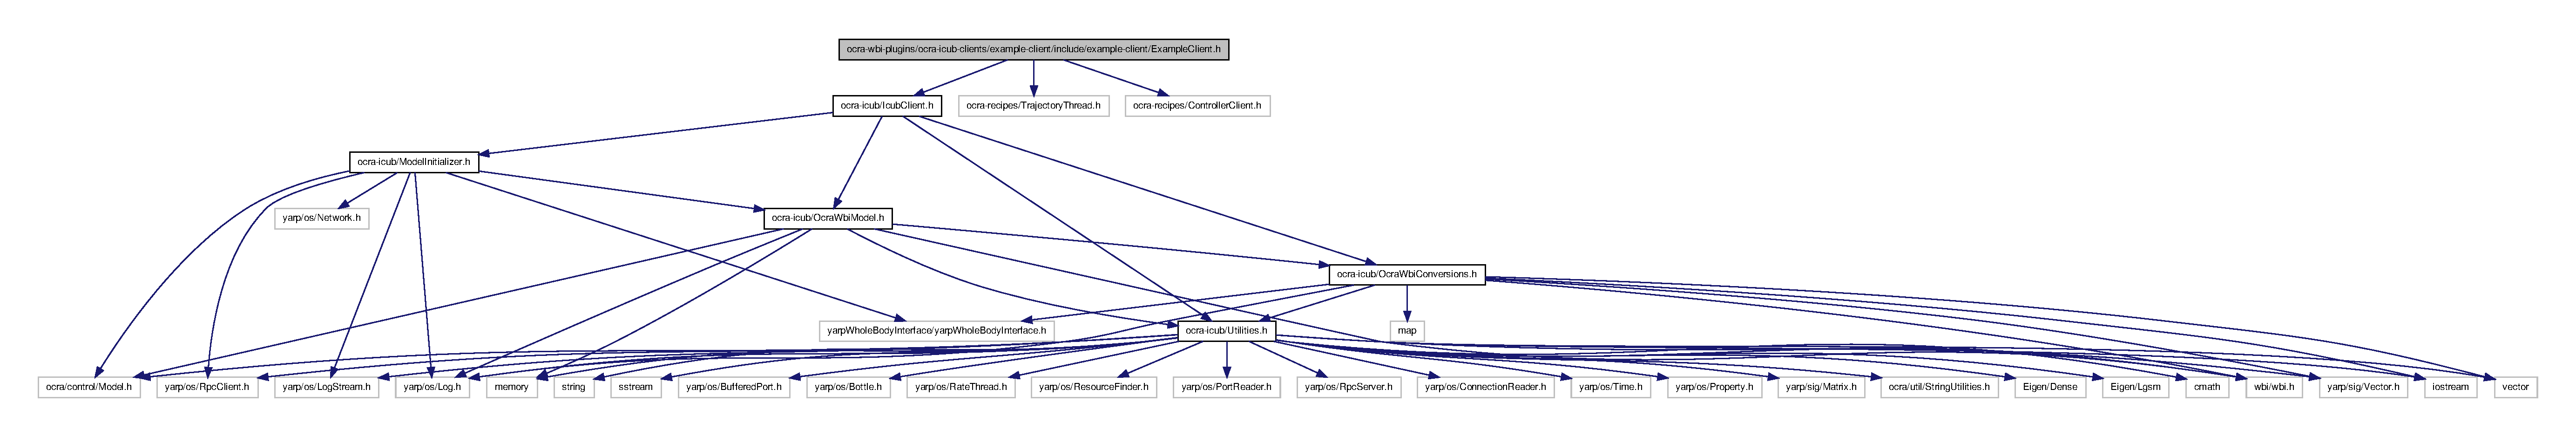
\includegraphics[width=350pt]{ExampleClient_8h__incl}
\end{center}
\end{figure}
\-This graph shows which files directly or indirectly include this file\-:
\nopagebreak
\begin{figure}[H]
\begin{center}
\leavevmode
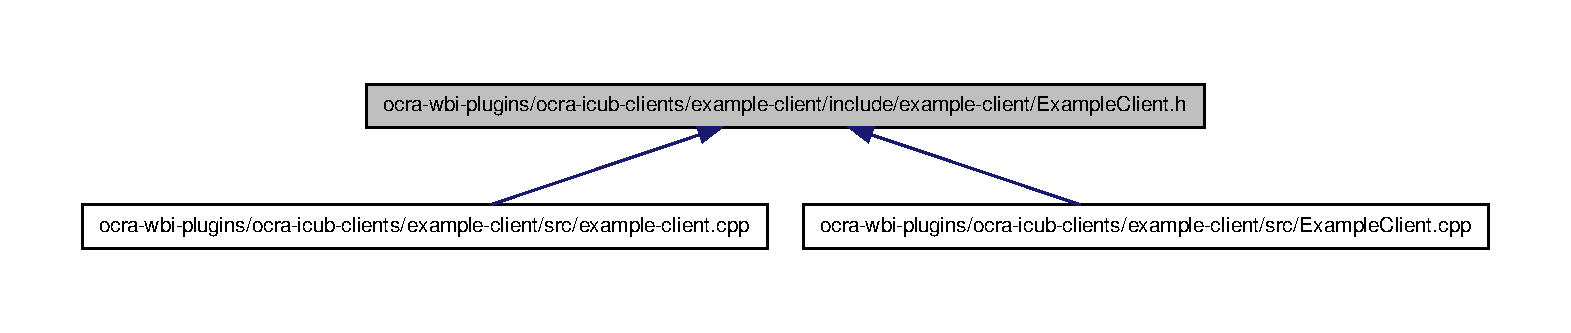
\includegraphics[width=350pt]{ExampleClient_8h__dep__incl}
\end{center}
\end{figure}
\subsection*{\-Classes}
\begin{DoxyCompactItemize}
\item 
class \hyperlink{classExampleClient}{\-Example\-Client}
\end{DoxyCompactItemize}

\hypertarget{example-client_8cpp}{\section{ocra-\/wbi-\/plugins/ocra-\/icub-\/clients/example-\/client/src/example-\/client.cpp \-File \-Reference}
\label{example-client_8cpp}\index{ocra-\/wbi-\/plugins/ocra-\/icub-\/clients/example-\/client/src/example-\/client.\-cpp@{ocra-\/wbi-\/plugins/ocra-\/icub-\/clients/example-\/client/src/example-\/client.\-cpp}}
}
{\ttfamily \#include $<$yarp/os/\-Resource\-Finder.\-h$>$}\*
{\ttfamily \#include $<$yarp/os/\-Network.\-h$>$}\*
{\ttfamily \#include $<$yarp/os/\-Log.\-h$>$}\*
{\ttfamily \#include $<$yarp/os/\-Log\-Stream.\-h$>$}\*
{\ttfamily \#include $<$yarp/os/\-Time.\-h$>$}\*
{\ttfamily \#include \char`\"{}example-\/client/\-Example\-Client.\-h\char`\"{}}\*
{\ttfamily \#include $<$ocra-\/icub/\-Icub\-Client.\-h$>$}\*
{\ttfamily \#include $<$ocra-\/recipes/\-Controller\-Client.\-h$>$}\*
{\ttfamily \#include $<$ocra-\/recipes/\-Client\-Manager.\-h$>$}\*
\-Include dependency graph for example-\/client.cpp\-:\nopagebreak
\begin{figure}[H]
\begin{center}
\leavevmode
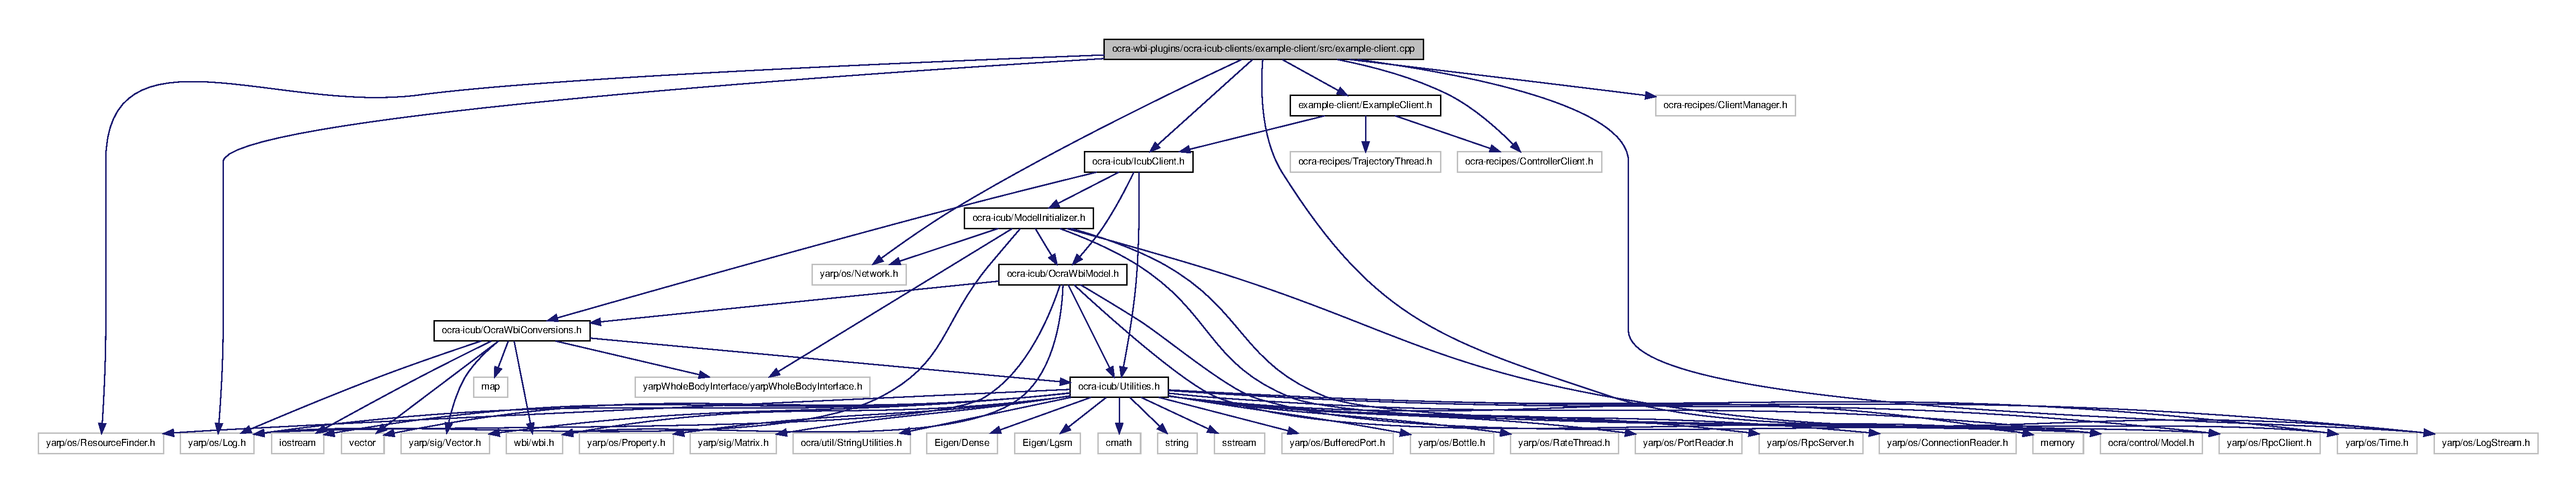
\includegraphics[width=350pt]{example-client_8cpp__incl}
\end{center}
\end{figure}
\subsection*{\-Functions}
\begin{DoxyCompactItemize}
\item 
int \hyperlink{example-client_8cpp_a0ddf1224851353fc92bfbff6f499fa97}{main} (int argc, char $\ast$argv\mbox{[}$\,$\mbox{]})
\end{DoxyCompactItemize}


\subsection{\-Detailed \-Description}
\begin{DoxyAuthor}{\-Author}
\mbox{[}\-Ryan \-Lober\mbox{]}(\href{http://www.ryanlober.com}{\tt http\-://www.\-ryanlober.\-com}) 

\mbox{[}\-Antoine \-Hoarau\mbox{]}(\href{http://ahoarau.github.io}{\tt http\-://ahoarau.\-github.\-io}) 
\end{DoxyAuthor}
\begin{DoxyDate}{\-Date}
\-Feb 2016 
\end{DoxyDate}
\begin{DoxyCopyright}{\-Copyright}
\-G\-N\-U \-General \-Public \-License. 
\end{DoxyCopyright}


\subsection{\-Function \-Documentation}
\hypertarget{example-client_8cpp_a0ddf1224851353fc92bfbff6f499fa97}{\index{example-\/client.\-cpp@{example-\/client.\-cpp}!main@{main}}
\index{main@{main}!example-client.cpp@{example-\/client.\-cpp}}
\subsubsection[{main}]{\setlength{\rightskip}{0pt plus 5cm}int {\bf main} (
\begin{DoxyParamCaption}
\item[{int}]{argc, }
\item[{char $\ast$}]{argv\mbox{[}$\,$\mbox{]}}
\end{DoxyParamCaption}
)}}\label{example-client_8cpp_a0ddf1224851353fc92bfbff6f499fa97}

\hypertarget{ExampleClient_8cpp}{\section{ocra-\/wbi-\/plugins/ocra-\/icub-\/clients/example-\/client/src/\-Example\-Client.cpp \-File \-Reference}
\label{ExampleClient_8cpp}\index{ocra-\/wbi-\/plugins/ocra-\/icub-\/clients/example-\/client/src/\-Example\-Client.\-cpp@{ocra-\/wbi-\/plugins/ocra-\/icub-\/clients/example-\/client/src/\-Example\-Client.\-cpp}}
}
{\ttfamily \#include \char`\"{}example-\/client/\-Example\-Client.\-h\char`\"{}}\*
\-Include dependency graph for \-Example\-Client.\-cpp\-:\nopagebreak
\begin{figure}[H]
\begin{center}
\leavevmode
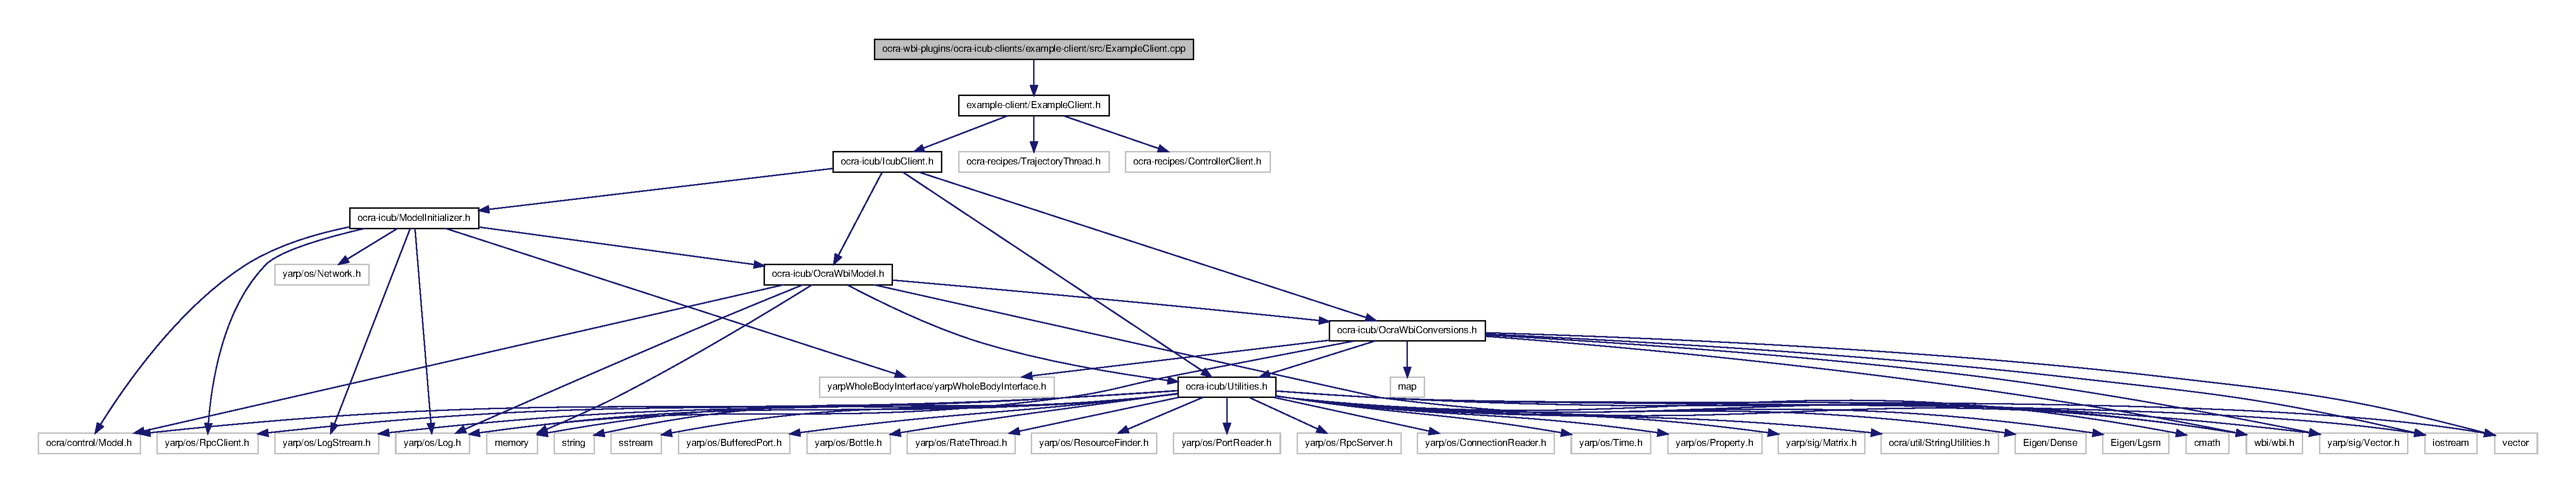
\includegraphics[width=350pt]{ExampleClient_8cpp__incl}
\end{center}
\end{figure}

\hypertarget{SittingDemoClient_8h}{\section{ocra-\/wbi-\/plugins/ocra-\/icub-\/clients/sitting-\/demo/include/sitting-\/demo/\-Sitting\-Demo\-Client.h \-File \-Reference}
\label{SittingDemoClient_8h}\index{ocra-\/wbi-\/plugins/ocra-\/icub-\/clients/sitting-\/demo/include/sitting-\/demo/\-Sitting\-Demo\-Client.\-h@{ocra-\/wbi-\/plugins/ocra-\/icub-\/clients/sitting-\/demo/include/sitting-\/demo/\-Sitting\-Demo\-Client.\-h}}
}
{\ttfamily \#include $<$ocra-\/icub/\-Icub\-Client.\-h$>$}\*
{\ttfamily \#include $<$ocra-\/recipes/\-Trajectory\-Thread.\-h$>$}\*
{\ttfamily \#include $<$ocra-\/recipes/\-Controller\-Client.\-h$>$}\*
\-Include dependency graph for \-Sitting\-Demo\-Client.\-h\-:\nopagebreak
\begin{figure}[H]
\begin{center}
\leavevmode
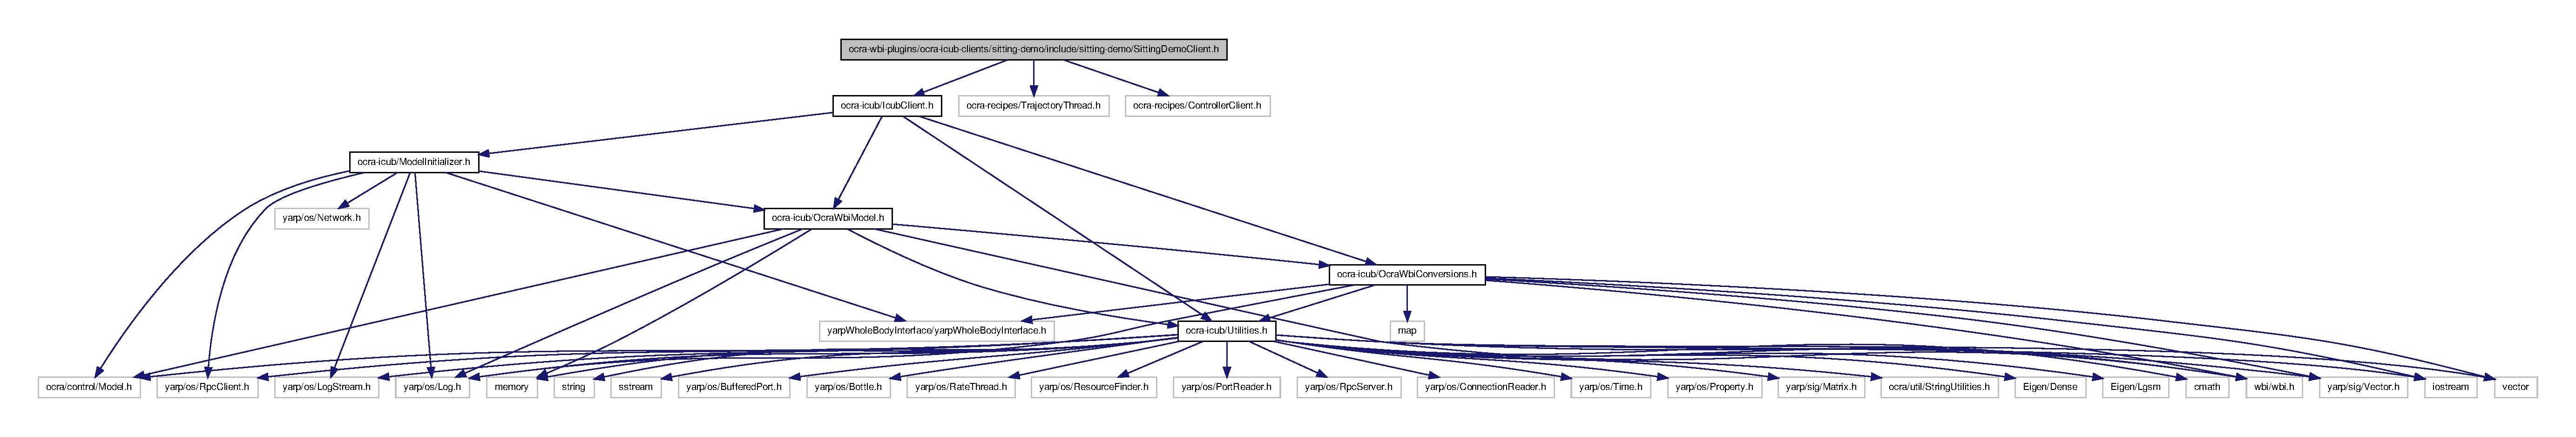
\includegraphics[width=350pt]{SittingDemoClient_8h__incl}
\end{center}
\end{figure}
\-This graph shows which files directly or indirectly include this file\-:\nopagebreak
\begin{figure}[H]
\begin{center}
\leavevmode
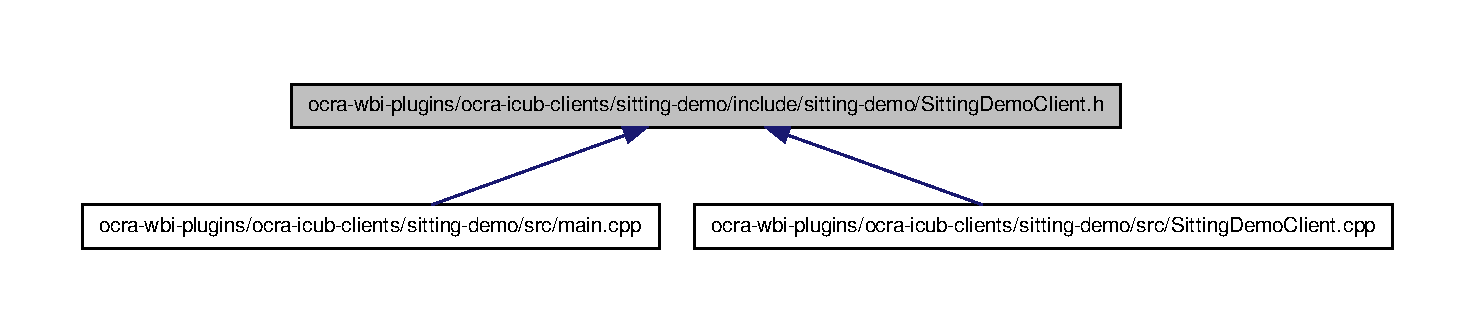
\includegraphics[width=350pt]{SittingDemoClient_8h__dep__incl}
\end{center}
\end{figure}
\subsection*{\-Classes}
\begin{DoxyCompactItemize}
\item 
class \hyperlink{classSittingDemoClient}{\-Sitting\-Demo\-Client}
\end{DoxyCompactItemize}

\hypertarget{SittingDemoClient_8cpp}{\section{ocra-\/wbi-\/plugins/ocra-\/icub-\/clients/sitting-\/demo/src/\-Sitting\-Demo\-Client.cpp \-File \-Reference}
\label{SittingDemoClient_8cpp}\index{ocra-\/wbi-\/plugins/ocra-\/icub-\/clients/sitting-\/demo/src/\-Sitting\-Demo\-Client.\-cpp@{ocra-\/wbi-\/plugins/ocra-\/icub-\/clients/sitting-\/demo/src/\-Sitting\-Demo\-Client.\-cpp}}
}
{\ttfamily \#include \char`\"{}sitting-\/demo/\-Sitting\-Demo\-Client.\-h\char`\"{}}\*
\-Include dependency graph for \-Sitting\-Demo\-Client.\-cpp\-:\nopagebreak
\begin{figure}[H]
\begin{center}
\leavevmode
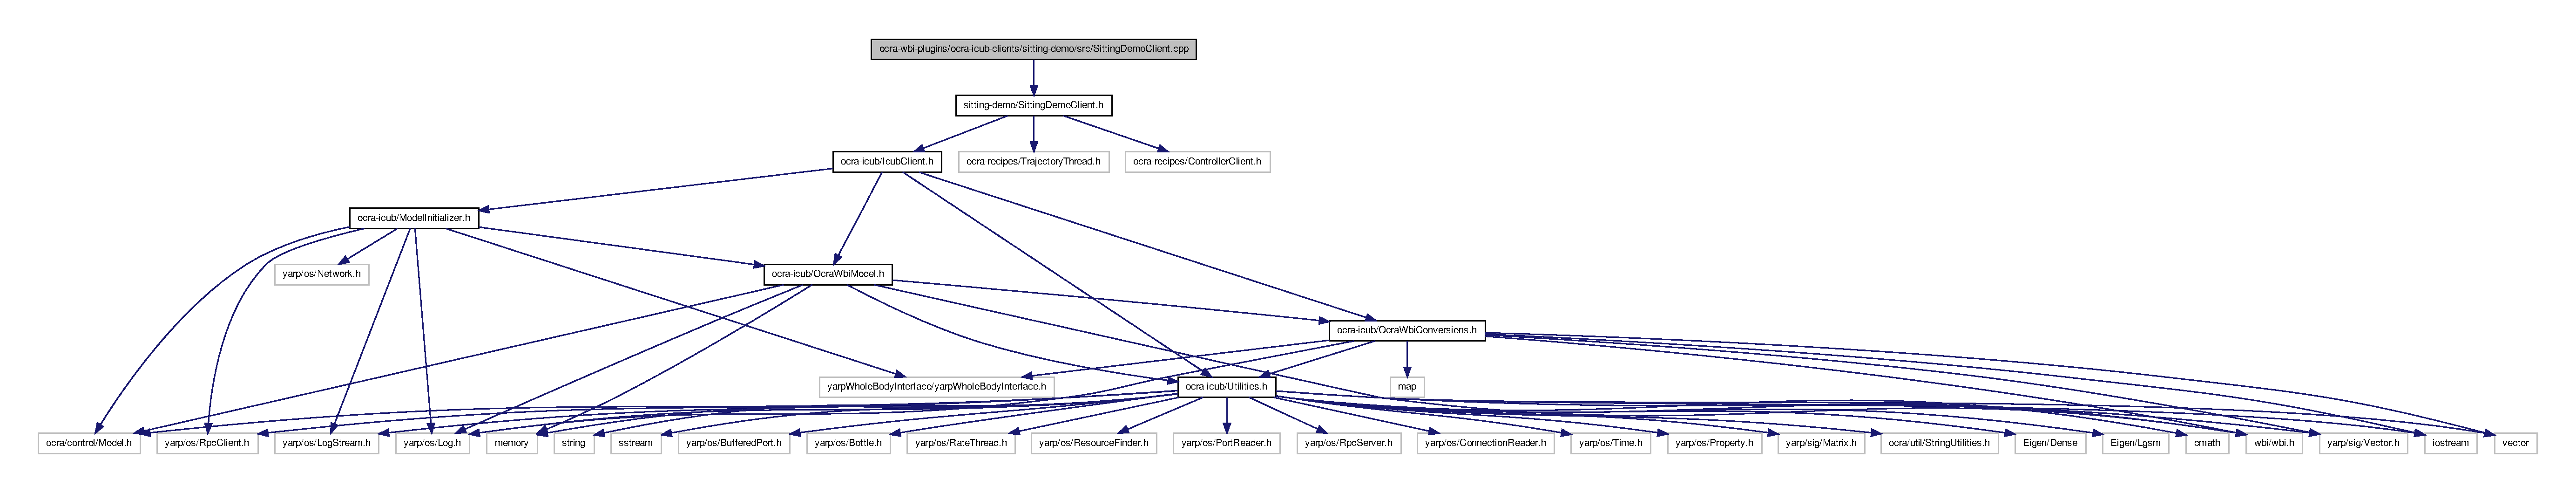
\includegraphics[width=350pt]{SittingDemoClient_8cpp__incl}
\end{center}
\end{figure}

\hypertarget{StandingDemoClient_8h}{\section{ocra-\/wbi-\/plugins/ocra-\/icub-\/clients/standing-\/demo/include/standing-\/demo/\-Standing\-Demo\-Client.h \-File \-Reference}
\label{StandingDemoClient_8h}\index{ocra-\/wbi-\/plugins/ocra-\/icub-\/clients/standing-\/demo/include/standing-\/demo/\-Standing\-Demo\-Client.\-h@{ocra-\/wbi-\/plugins/ocra-\/icub-\/clients/standing-\/demo/include/standing-\/demo/\-Standing\-Demo\-Client.\-h}}
}
{\ttfamily \#include $<$ocra-\/icub/\-Icub\-Client.\-h$>$}\*
{\ttfamily \#include $<$ocra-\/recipes/\-Trajectory\-Thread.\-h$>$}\*
{\ttfamily \#include $<$ocra-\/recipes/\-Controller\-Client.\-h$>$}\*
\-Include dependency graph for \-Standing\-Demo\-Client.\-h\-:
\nopagebreak
\begin{figure}[H]
\begin{center}
\leavevmode
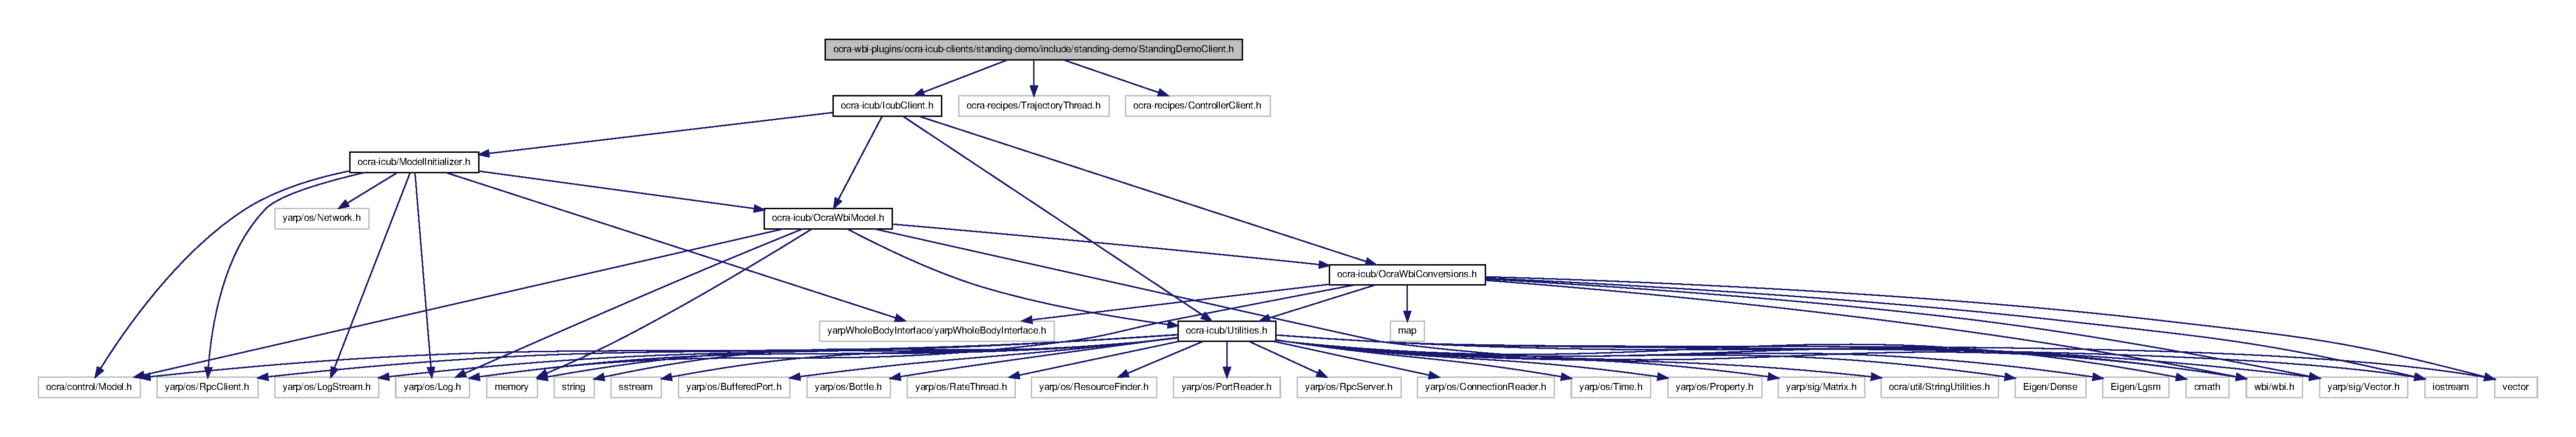
\includegraphics[width=350pt]{StandingDemoClient_8h__incl}
\end{center}
\end{figure}
\-This graph shows which files directly or indirectly include this file\-:
\nopagebreak
\begin{figure}[H]
\begin{center}
\leavevmode
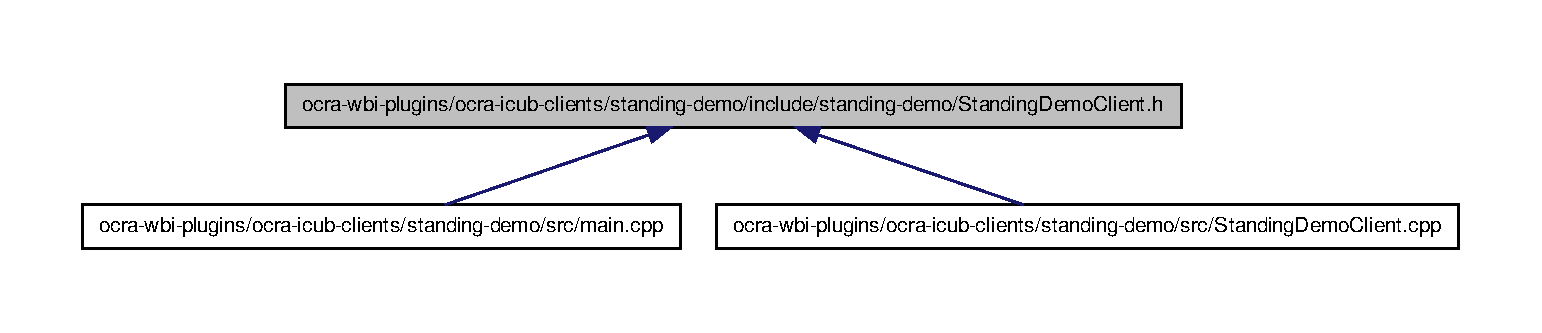
\includegraphics[width=350pt]{StandingDemoClient_8h__dep__incl}
\end{center}
\end{figure}
\subsection*{\-Classes}
\begin{DoxyCompactItemize}
\item 
class \hyperlink{classStandingDemoClient}{\-Standing\-Demo\-Client}
\end{DoxyCompactItemize}

\hypertarget{StandingDemoClient_8cpp}{\section{ocra-\/wbi-\/plugins/ocra-\/icub-\/clients/standing-\/demo/src/\-Standing\-Demo\-Client.cpp \-File \-Reference}
\label{StandingDemoClient_8cpp}\index{ocra-\/wbi-\/plugins/ocra-\/icub-\/clients/standing-\/demo/src/\-Standing\-Demo\-Client.\-cpp@{ocra-\/wbi-\/plugins/ocra-\/icub-\/clients/standing-\/demo/src/\-Standing\-Demo\-Client.\-cpp}}
}
{\ttfamily \#include \char`\"{}standing-\/demo/\-Standing\-Demo\-Client.\-h\char`\"{}}\*
\-Include dependency graph for \-Standing\-Demo\-Client.\-cpp\-:
\nopagebreak
\begin{figure}[H]
\begin{center}
\leavevmode
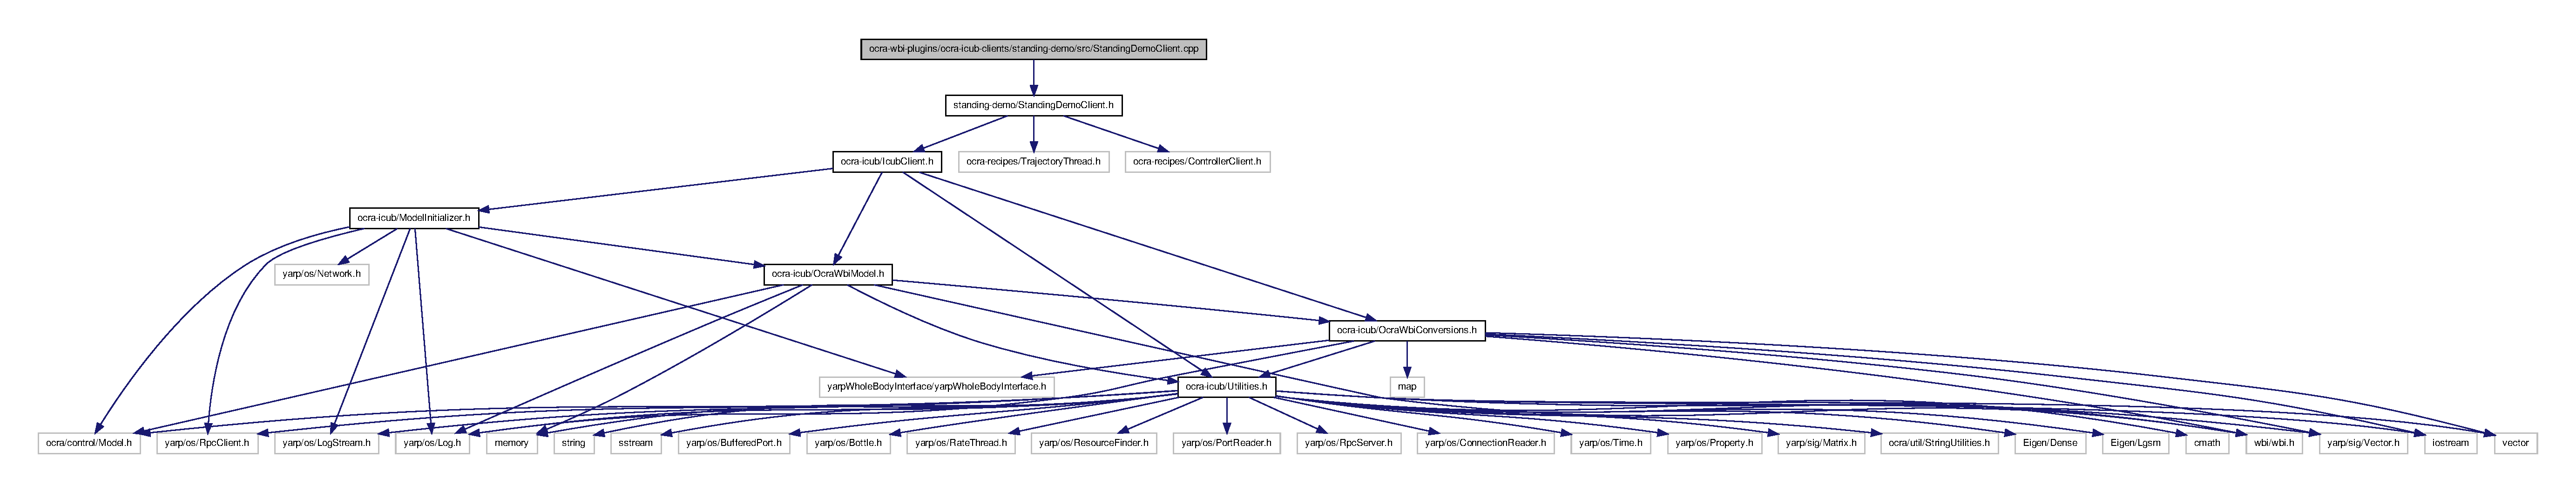
\includegraphics[width=350pt]{StandingDemoClient_8cpp__incl}
\end{center}
\end{figure}

\hypertarget{SteppingDemoClient_8h}{\section{ocra-\/wbi-\/plugins/ocra-\/icub-\/clients/stepping-\/demo/include/stepping-\/demo/\-Stepping\-Demo\-Client.h \-File \-Reference}
\label{SteppingDemoClient_8h}\index{ocra-\/wbi-\/plugins/ocra-\/icub-\/clients/stepping-\/demo/include/stepping-\/demo/\-Stepping\-Demo\-Client.\-h@{ocra-\/wbi-\/plugins/ocra-\/icub-\/clients/stepping-\/demo/include/stepping-\/demo/\-Stepping\-Demo\-Client.\-h}}
}
{\ttfamily \#include $<$ocra-\/icub/\-Icub\-Client.\-h$>$}\*
{\ttfamily \#include $<$ocra-\/recipes/\-Trajectory\-Thread.\-h$>$}\*
{\ttfamily \#include $<$ocra-\/recipes/\-Controller\-Client.\-h$>$}\*
{\ttfamily \#include $<$ocra/util/\-Errors\-Helper.\-h$>$}\*
\-Include dependency graph for \-Stepping\-Demo\-Client.\-h\-:
\nopagebreak
\begin{figure}[H]
\begin{center}
\leavevmode
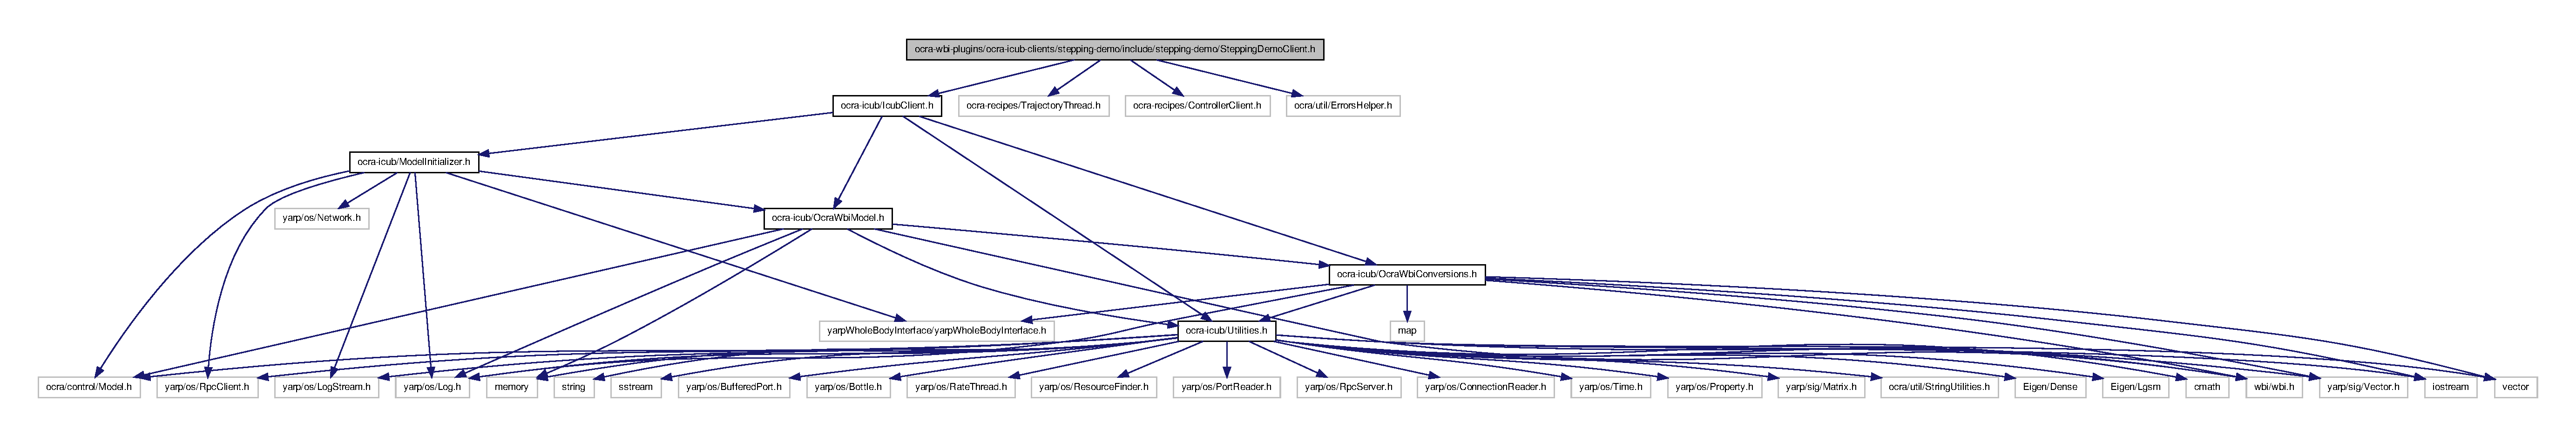
\includegraphics[width=350pt]{SteppingDemoClient_8h__incl}
\end{center}
\end{figure}
\-This graph shows which files directly or indirectly include this file\-:
\nopagebreak
\begin{figure}[H]
\begin{center}
\leavevmode
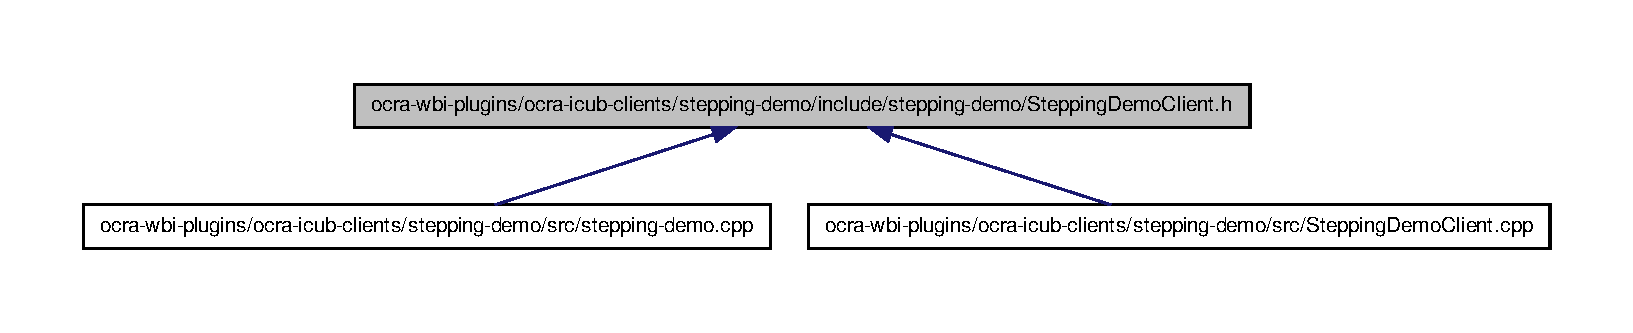
\includegraphics[width=350pt]{SteppingDemoClient_8h__dep__incl}
\end{center}
\end{figure}
\subsection*{\-Classes}
\begin{DoxyCompactItemize}
\item 
struct \hyperlink{structWalkingParams}{\-Walking\-Params}
\item 
class \hyperlink{classSteppingDemoClient}{\-Stepping\-Demo\-Client}
\end{DoxyCompactItemize}
\subsection*{\-Enumerations}
\begin{DoxyCompactItemize}
\item 
enum \hyperlink{SteppingDemoClient_8h_ac0c3848a609566394821d9826e0fdd5b}{\-C\-O\-M\-\_\-\-S\-U\-P\-P\-O\-R\-T\-\_\-\-P\-O\-S\-I\-T\-I\-O\-N} \{ \hyperlink{SteppingDemoClient_8h_ac0c3848a609566394821d9826e0fdd5ba07cd79ee915be269a43f655f31cd3ccf}{\-L\-E\-F\-T\-\_\-\-F\-O\-O\-T\-\_\-\-X\-Y}, 
\hyperlink{SteppingDemoClient_8h_ac0c3848a609566394821d9826e0fdd5ba273605381ab0231d2abb4a8096faabfd}{\-R\-I\-G\-H\-T\-\_\-\-F\-O\-O\-T\-\_\-\-X\-Y}, 
\hyperlink{SteppingDemoClient_8h_ac0c3848a609566394821d9826e0fdd5bad32a9ea5bb598218529abf1a5b9b50cf}{\-C\-E\-N\-T\-E\-R\-E\-D\-\_\-\-B\-E\-T\-W\-E\-E\-N\-\_\-\-F\-E\-E\-T\-\_\-\-X\-Y}
 \}
\item 
enum \hyperlink{SteppingDemoClient_8h_af2a8507bf21c3ce9b0e67a23381251c6}{\-C\-O\-N\-T\-R\-O\-L\-\_\-\-P\-H\-A\-S\-E} \{ \hyperlink{SteppingDemoClient_8h_af2a8507bf21c3ce9b0e67a23381251c6afe7fc4a2f5d6778bbb96f412be37d63c}{\-M\-O\-V\-E\-\_\-\-T\-O\-\_\-\-L\-E\-F\-T\-\_\-\-S\-U\-P\-P\-O\-R\-T}, 
\hyperlink{SteppingDemoClient_8h_af2a8507bf21c3ce9b0e67a23381251c6a3b4335037acf972dd5d60348ca20d394}{\-M\-O\-V\-E\-\_\-\-T\-O\-\_\-\-R\-I\-G\-H\-T\-\_\-\-S\-U\-P\-P\-O\-R\-T}, 
\hyperlink{SteppingDemoClient_8h_af2a8507bf21c3ce9b0e67a23381251c6a362d8557e44bcc19f6b4d9096bb54401}{\-M\-O\-V\-E\-\_\-\-T\-O\-\_\-\-D\-O\-U\-B\-L\-E\-\_\-\-S\-U\-P\-P\-O\-R\-T}, 
\hyperlink{SteppingDemoClient_8h_af2a8507bf21c3ce9b0e67a23381251c6a4ff6c6ae9503ea4bca745c7d7819523e}{\-S\-T\-E\-P\-\_\-\-F\-O\-R\-W\-A\-R\-D}
 \}
\item 
enum \hyperlink{SteppingDemoClient_8h_ab0673d7f17cdd57b8fa124abb330287f}{\-F\-O\-O\-T\-\_\-\-C\-O\-N\-T\-A\-C\-T\-S} \{ \hyperlink{SteppingDemoClient_8h_ab0673d7f17cdd57b8fa124abb330287fa7760daad9db1ede8c57b06189deca9f3}{\-L\-E\-F\-T\-\_\-\-F\-O\-O\-T}, 
\hyperlink{SteppingDemoClient_8h_ab0673d7f17cdd57b8fa124abb330287face119c66af60ac0781b137aa87d7be62}{\-R\-I\-G\-H\-T\-\_\-\-F\-O\-O\-T}
 \}
\item 
enum \hyperlink{SteppingDemoClient_8h_abd6d177d63e98aa1b4ed4b8329e2a379}{\-M\-O\-T\-I\-O\-N\-\_\-\-T\-Y\-P\-E} \{ \hyperlink{SteppingDemoClient_8h_abd6d177d63e98aa1b4ed4b8329e2a379a55b57dce74f14a62104ae66e62789eb3}{\-L\-E\-F\-T\-\_\-\-T\-O\-\_\-\-R\-I\-G\-H\-T}, 
\hyperlink{SteppingDemoClient_8h_abd6d177d63e98aa1b4ed4b8329e2a379ada7017955bb1db9f0954017358028fa6}{\-S\-T\-A\-T\-I\-C\-\_\-\-W\-A\-L\-K\-I\-N\-G}
 \}
\end{DoxyCompactItemize}


\subsection{\-Enumeration \-Type \-Documentation}
\hypertarget{SteppingDemoClient_8h_ac0c3848a609566394821d9826e0fdd5b}{\index{\-Stepping\-Demo\-Client.\-h@{\-Stepping\-Demo\-Client.\-h}!\-C\-O\-M\-\_\-\-S\-U\-P\-P\-O\-R\-T\-\_\-\-P\-O\-S\-I\-T\-I\-O\-N@{\-C\-O\-M\-\_\-\-S\-U\-P\-P\-O\-R\-T\-\_\-\-P\-O\-S\-I\-T\-I\-O\-N}}
\index{\-C\-O\-M\-\_\-\-S\-U\-P\-P\-O\-R\-T\-\_\-\-P\-O\-S\-I\-T\-I\-O\-N@{\-C\-O\-M\-\_\-\-S\-U\-P\-P\-O\-R\-T\-\_\-\-P\-O\-S\-I\-T\-I\-O\-N}!SteppingDemoClient.h@{\-Stepping\-Demo\-Client.\-h}}
\subsubsection[{\-C\-O\-M\-\_\-\-S\-U\-P\-P\-O\-R\-T\-\_\-\-P\-O\-S\-I\-T\-I\-O\-N}]{\setlength{\rightskip}{0pt plus 5cm}enum {\bf \-C\-O\-M\-\_\-\-S\-U\-P\-P\-O\-R\-T\-\_\-\-P\-O\-S\-I\-T\-I\-O\-N}}}\label{SteppingDemoClient_8h_ac0c3848a609566394821d9826e0fdd5b}
\begin{Desc}
\item[\-Enumerator\-: ]\par
\begin{description}
\index{\-L\-E\-F\-T\-\_\-\-F\-O\-O\-T\-\_\-\-X\-Y@{\-L\-E\-F\-T\-\_\-\-F\-O\-O\-T\-\_\-\-X\-Y}!\-Stepping\-Demo\-Client.\-h@{\-Stepping\-Demo\-Client.\-h}}\index{\-Stepping\-Demo\-Client.\-h@{\-Stepping\-Demo\-Client.\-h}!\-L\-E\-F\-T\-\_\-\-F\-O\-O\-T\-\_\-\-X\-Y@{\-L\-E\-F\-T\-\_\-\-F\-O\-O\-T\-\_\-\-X\-Y}}\item[{\em 
\hypertarget{SteppingDemoClient_8h_ac0c3848a609566394821d9826e0fdd5ba07cd79ee915be269a43f655f31cd3ccf}{\-L\-E\-F\-T\-\_\-\-F\-O\-O\-T\-\_\-\-X\-Y}\label{SteppingDemoClient_8h_ac0c3848a609566394821d9826e0fdd5ba07cd79ee915be269a43f655f31cd3ccf}
}]\index{\-R\-I\-G\-H\-T\-\_\-\-F\-O\-O\-T\-\_\-\-X\-Y@{\-R\-I\-G\-H\-T\-\_\-\-F\-O\-O\-T\-\_\-\-X\-Y}!\-Stepping\-Demo\-Client.\-h@{\-Stepping\-Demo\-Client.\-h}}\index{\-Stepping\-Demo\-Client.\-h@{\-Stepping\-Demo\-Client.\-h}!\-R\-I\-G\-H\-T\-\_\-\-F\-O\-O\-T\-\_\-\-X\-Y@{\-R\-I\-G\-H\-T\-\_\-\-F\-O\-O\-T\-\_\-\-X\-Y}}\item[{\em 
\hypertarget{SteppingDemoClient_8h_ac0c3848a609566394821d9826e0fdd5ba273605381ab0231d2abb4a8096faabfd}{\-R\-I\-G\-H\-T\-\_\-\-F\-O\-O\-T\-\_\-\-X\-Y}\label{SteppingDemoClient_8h_ac0c3848a609566394821d9826e0fdd5ba273605381ab0231d2abb4a8096faabfd}
}]\index{\-C\-E\-N\-T\-E\-R\-E\-D\-\_\-\-B\-E\-T\-W\-E\-E\-N\-\_\-\-F\-E\-E\-T\-\_\-\-X\-Y@{\-C\-E\-N\-T\-E\-R\-E\-D\-\_\-\-B\-E\-T\-W\-E\-E\-N\-\_\-\-F\-E\-E\-T\-\_\-\-X\-Y}!\-Stepping\-Demo\-Client.\-h@{\-Stepping\-Demo\-Client.\-h}}\index{\-Stepping\-Demo\-Client.\-h@{\-Stepping\-Demo\-Client.\-h}!\-C\-E\-N\-T\-E\-R\-E\-D\-\_\-\-B\-E\-T\-W\-E\-E\-N\-\_\-\-F\-E\-E\-T\-\_\-\-X\-Y@{\-C\-E\-N\-T\-E\-R\-E\-D\-\_\-\-B\-E\-T\-W\-E\-E\-N\-\_\-\-F\-E\-E\-T\-\_\-\-X\-Y}}\item[{\em 
\hypertarget{SteppingDemoClient_8h_ac0c3848a609566394821d9826e0fdd5bad32a9ea5bb598218529abf1a5b9b50cf}{\-C\-E\-N\-T\-E\-R\-E\-D\-\_\-\-B\-E\-T\-W\-E\-E\-N\-\_\-\-F\-E\-E\-T\-\_\-\-X\-Y}\label{SteppingDemoClient_8h_ac0c3848a609566394821d9826e0fdd5bad32a9ea5bb598218529abf1a5b9b50cf}
}]\end{description}
\end{Desc}

\hypertarget{SteppingDemoClient_8h_af2a8507bf21c3ce9b0e67a23381251c6}{\index{\-Stepping\-Demo\-Client.\-h@{\-Stepping\-Demo\-Client.\-h}!\-C\-O\-N\-T\-R\-O\-L\-\_\-\-P\-H\-A\-S\-E@{\-C\-O\-N\-T\-R\-O\-L\-\_\-\-P\-H\-A\-S\-E}}
\index{\-C\-O\-N\-T\-R\-O\-L\-\_\-\-P\-H\-A\-S\-E@{\-C\-O\-N\-T\-R\-O\-L\-\_\-\-P\-H\-A\-S\-E}!SteppingDemoClient.h@{\-Stepping\-Demo\-Client.\-h}}
\subsubsection[{\-C\-O\-N\-T\-R\-O\-L\-\_\-\-P\-H\-A\-S\-E}]{\setlength{\rightskip}{0pt plus 5cm}enum {\bf \-C\-O\-N\-T\-R\-O\-L\-\_\-\-P\-H\-A\-S\-E}}}\label{SteppingDemoClient_8h_af2a8507bf21c3ce9b0e67a23381251c6}
\begin{Desc}
\item[\-Enumerator\-: ]\par
\begin{description}
\index{\-M\-O\-V\-E\-\_\-\-T\-O\-\_\-\-L\-E\-F\-T\-\_\-\-S\-U\-P\-P\-O\-R\-T@{\-M\-O\-V\-E\-\_\-\-T\-O\-\_\-\-L\-E\-F\-T\-\_\-\-S\-U\-P\-P\-O\-R\-T}!\-Stepping\-Demo\-Client.\-h@{\-Stepping\-Demo\-Client.\-h}}\index{\-Stepping\-Demo\-Client.\-h@{\-Stepping\-Demo\-Client.\-h}!\-M\-O\-V\-E\-\_\-\-T\-O\-\_\-\-L\-E\-F\-T\-\_\-\-S\-U\-P\-P\-O\-R\-T@{\-M\-O\-V\-E\-\_\-\-T\-O\-\_\-\-L\-E\-F\-T\-\_\-\-S\-U\-P\-P\-O\-R\-T}}\item[{\em 
\hypertarget{SteppingDemoClient_8h_af2a8507bf21c3ce9b0e67a23381251c6afe7fc4a2f5d6778bbb96f412be37d63c}{\-M\-O\-V\-E\-\_\-\-T\-O\-\_\-\-L\-E\-F\-T\-\_\-\-S\-U\-P\-P\-O\-R\-T}\label{SteppingDemoClient_8h_af2a8507bf21c3ce9b0e67a23381251c6afe7fc4a2f5d6778bbb96f412be37d63c}
}]\index{\-M\-O\-V\-E\-\_\-\-T\-O\-\_\-\-R\-I\-G\-H\-T\-\_\-\-S\-U\-P\-P\-O\-R\-T@{\-M\-O\-V\-E\-\_\-\-T\-O\-\_\-\-R\-I\-G\-H\-T\-\_\-\-S\-U\-P\-P\-O\-R\-T}!\-Stepping\-Demo\-Client.\-h@{\-Stepping\-Demo\-Client.\-h}}\index{\-Stepping\-Demo\-Client.\-h@{\-Stepping\-Demo\-Client.\-h}!\-M\-O\-V\-E\-\_\-\-T\-O\-\_\-\-R\-I\-G\-H\-T\-\_\-\-S\-U\-P\-P\-O\-R\-T@{\-M\-O\-V\-E\-\_\-\-T\-O\-\_\-\-R\-I\-G\-H\-T\-\_\-\-S\-U\-P\-P\-O\-R\-T}}\item[{\em 
\hypertarget{SteppingDemoClient_8h_af2a8507bf21c3ce9b0e67a23381251c6a3b4335037acf972dd5d60348ca20d394}{\-M\-O\-V\-E\-\_\-\-T\-O\-\_\-\-R\-I\-G\-H\-T\-\_\-\-S\-U\-P\-P\-O\-R\-T}\label{SteppingDemoClient_8h_af2a8507bf21c3ce9b0e67a23381251c6a3b4335037acf972dd5d60348ca20d394}
}]\index{\-M\-O\-V\-E\-\_\-\-T\-O\-\_\-\-D\-O\-U\-B\-L\-E\-\_\-\-S\-U\-P\-P\-O\-R\-T@{\-M\-O\-V\-E\-\_\-\-T\-O\-\_\-\-D\-O\-U\-B\-L\-E\-\_\-\-S\-U\-P\-P\-O\-R\-T}!\-Stepping\-Demo\-Client.\-h@{\-Stepping\-Demo\-Client.\-h}}\index{\-Stepping\-Demo\-Client.\-h@{\-Stepping\-Demo\-Client.\-h}!\-M\-O\-V\-E\-\_\-\-T\-O\-\_\-\-D\-O\-U\-B\-L\-E\-\_\-\-S\-U\-P\-P\-O\-R\-T@{\-M\-O\-V\-E\-\_\-\-T\-O\-\_\-\-D\-O\-U\-B\-L\-E\-\_\-\-S\-U\-P\-P\-O\-R\-T}}\item[{\em 
\hypertarget{SteppingDemoClient_8h_af2a8507bf21c3ce9b0e67a23381251c6a362d8557e44bcc19f6b4d9096bb54401}{\-M\-O\-V\-E\-\_\-\-T\-O\-\_\-\-D\-O\-U\-B\-L\-E\-\_\-\-S\-U\-P\-P\-O\-R\-T}\label{SteppingDemoClient_8h_af2a8507bf21c3ce9b0e67a23381251c6a362d8557e44bcc19f6b4d9096bb54401}
}]\index{\-S\-T\-E\-P\-\_\-\-F\-O\-R\-W\-A\-R\-D@{\-S\-T\-E\-P\-\_\-\-F\-O\-R\-W\-A\-R\-D}!\-Stepping\-Demo\-Client.\-h@{\-Stepping\-Demo\-Client.\-h}}\index{\-Stepping\-Demo\-Client.\-h@{\-Stepping\-Demo\-Client.\-h}!\-S\-T\-E\-P\-\_\-\-F\-O\-R\-W\-A\-R\-D@{\-S\-T\-E\-P\-\_\-\-F\-O\-R\-W\-A\-R\-D}}\item[{\em 
\hypertarget{SteppingDemoClient_8h_af2a8507bf21c3ce9b0e67a23381251c6a4ff6c6ae9503ea4bca745c7d7819523e}{\-S\-T\-E\-P\-\_\-\-F\-O\-R\-W\-A\-R\-D}\label{SteppingDemoClient_8h_af2a8507bf21c3ce9b0e67a23381251c6a4ff6c6ae9503ea4bca745c7d7819523e}
}]\end{description}
\end{Desc}

\hypertarget{SteppingDemoClient_8h_ab0673d7f17cdd57b8fa124abb330287f}{\index{\-Stepping\-Demo\-Client.\-h@{\-Stepping\-Demo\-Client.\-h}!\-F\-O\-O\-T\-\_\-\-C\-O\-N\-T\-A\-C\-T\-S@{\-F\-O\-O\-T\-\_\-\-C\-O\-N\-T\-A\-C\-T\-S}}
\index{\-F\-O\-O\-T\-\_\-\-C\-O\-N\-T\-A\-C\-T\-S@{\-F\-O\-O\-T\-\_\-\-C\-O\-N\-T\-A\-C\-T\-S}!SteppingDemoClient.h@{\-Stepping\-Demo\-Client.\-h}}
\subsubsection[{\-F\-O\-O\-T\-\_\-\-C\-O\-N\-T\-A\-C\-T\-S}]{\setlength{\rightskip}{0pt plus 5cm}enum {\bf \-F\-O\-O\-T\-\_\-\-C\-O\-N\-T\-A\-C\-T\-S}}}\label{SteppingDemoClient_8h_ab0673d7f17cdd57b8fa124abb330287f}
\begin{Desc}
\item[\-Enumerator\-: ]\par
\begin{description}
\index{\-L\-E\-F\-T\-\_\-\-F\-O\-O\-T@{\-L\-E\-F\-T\-\_\-\-F\-O\-O\-T}!\-Stepping\-Demo\-Client.\-h@{\-Stepping\-Demo\-Client.\-h}}\index{\-Stepping\-Demo\-Client.\-h@{\-Stepping\-Demo\-Client.\-h}!\-L\-E\-F\-T\-\_\-\-F\-O\-O\-T@{\-L\-E\-F\-T\-\_\-\-F\-O\-O\-T}}\item[{\em 
\hypertarget{SteppingDemoClient_8h_ab0673d7f17cdd57b8fa124abb330287fa7760daad9db1ede8c57b06189deca9f3}{\-L\-E\-F\-T\-\_\-\-F\-O\-O\-T}\label{SteppingDemoClient_8h_ab0673d7f17cdd57b8fa124abb330287fa7760daad9db1ede8c57b06189deca9f3}
}]\index{\-R\-I\-G\-H\-T\-\_\-\-F\-O\-O\-T@{\-R\-I\-G\-H\-T\-\_\-\-F\-O\-O\-T}!\-Stepping\-Demo\-Client.\-h@{\-Stepping\-Demo\-Client.\-h}}\index{\-Stepping\-Demo\-Client.\-h@{\-Stepping\-Demo\-Client.\-h}!\-R\-I\-G\-H\-T\-\_\-\-F\-O\-O\-T@{\-R\-I\-G\-H\-T\-\_\-\-F\-O\-O\-T}}\item[{\em 
\hypertarget{SteppingDemoClient_8h_ab0673d7f17cdd57b8fa124abb330287face119c66af60ac0781b137aa87d7be62}{\-R\-I\-G\-H\-T\-\_\-\-F\-O\-O\-T}\label{SteppingDemoClient_8h_ab0673d7f17cdd57b8fa124abb330287face119c66af60ac0781b137aa87d7be62}
}]\end{description}
\end{Desc}

\hypertarget{SteppingDemoClient_8h_abd6d177d63e98aa1b4ed4b8329e2a379}{\index{\-Stepping\-Demo\-Client.\-h@{\-Stepping\-Demo\-Client.\-h}!\-M\-O\-T\-I\-O\-N\-\_\-\-T\-Y\-P\-E@{\-M\-O\-T\-I\-O\-N\-\_\-\-T\-Y\-P\-E}}
\index{\-M\-O\-T\-I\-O\-N\-\_\-\-T\-Y\-P\-E@{\-M\-O\-T\-I\-O\-N\-\_\-\-T\-Y\-P\-E}!SteppingDemoClient.h@{\-Stepping\-Demo\-Client.\-h}}
\subsubsection[{\-M\-O\-T\-I\-O\-N\-\_\-\-T\-Y\-P\-E}]{\setlength{\rightskip}{0pt plus 5cm}enum {\bf \-M\-O\-T\-I\-O\-N\-\_\-\-T\-Y\-P\-E}}}\label{SteppingDemoClient_8h_abd6d177d63e98aa1b4ed4b8329e2a379}
\begin{Desc}
\item[\-Enumerator\-: ]\par
\begin{description}
\index{\-L\-E\-F\-T\-\_\-\-T\-O\-\_\-\-R\-I\-G\-H\-T@{\-L\-E\-F\-T\-\_\-\-T\-O\-\_\-\-R\-I\-G\-H\-T}!\-Stepping\-Demo\-Client.\-h@{\-Stepping\-Demo\-Client.\-h}}\index{\-Stepping\-Demo\-Client.\-h@{\-Stepping\-Demo\-Client.\-h}!\-L\-E\-F\-T\-\_\-\-T\-O\-\_\-\-R\-I\-G\-H\-T@{\-L\-E\-F\-T\-\_\-\-T\-O\-\_\-\-R\-I\-G\-H\-T}}\item[{\em 
\hypertarget{SteppingDemoClient_8h_abd6d177d63e98aa1b4ed4b8329e2a379a55b57dce74f14a62104ae66e62789eb3}{\-L\-E\-F\-T\-\_\-\-T\-O\-\_\-\-R\-I\-G\-H\-T}\label{SteppingDemoClient_8h_abd6d177d63e98aa1b4ed4b8329e2a379a55b57dce74f14a62104ae66e62789eb3}
}]\index{\-S\-T\-A\-T\-I\-C\-\_\-\-W\-A\-L\-K\-I\-N\-G@{\-S\-T\-A\-T\-I\-C\-\_\-\-W\-A\-L\-K\-I\-N\-G}!\-Stepping\-Demo\-Client.\-h@{\-Stepping\-Demo\-Client.\-h}}\index{\-Stepping\-Demo\-Client.\-h@{\-Stepping\-Demo\-Client.\-h}!\-S\-T\-A\-T\-I\-C\-\_\-\-W\-A\-L\-K\-I\-N\-G@{\-S\-T\-A\-T\-I\-C\-\_\-\-W\-A\-L\-K\-I\-N\-G}}\item[{\em 
\hypertarget{SteppingDemoClient_8h_abd6d177d63e98aa1b4ed4b8329e2a379ada7017955bb1db9f0954017358028fa6}{\-S\-T\-A\-T\-I\-C\-\_\-\-W\-A\-L\-K\-I\-N\-G}\label{SteppingDemoClient_8h_abd6d177d63e98aa1b4ed4b8329e2a379ada7017955bb1db9f0954017358028fa6}
}]\end{description}
\end{Desc}


\hypertarget{stepping-demo_8cpp}{\section{ocra-\/wbi-\/plugins/ocra-\/icub-\/clients/stepping-\/demo/src/stepping-\/demo.cpp \-File \-Reference}
\label{stepping-demo_8cpp}\index{ocra-\/wbi-\/plugins/ocra-\/icub-\/clients/stepping-\/demo/src/stepping-\/demo.\-cpp@{ocra-\/wbi-\/plugins/ocra-\/icub-\/clients/stepping-\/demo/src/stepping-\/demo.\-cpp}}
}
{\ttfamily \#include $<$yarp/os/\-Resource\-Finder.\-h$>$}\*
{\ttfamily \#include $<$yarp/os/\-Network.\-h$>$}\*
{\ttfamily \#include $<$yarp/os/\-Log.\-h$>$}\*
{\ttfamily \#include $<$yarp/os/\-Log\-Stream.\-h$>$}\*
{\ttfamily \#include $<$yarp/os/\-Time.\-h$>$}\*
{\ttfamily \#include \char`\"{}stepping-\/demo/\-Stepping\-Demo\-Client.\-h\char`\"{}}\*
{\ttfamily \#include $<$ocra-\/icub/\-Icub\-Client.\-h$>$}\*
{\ttfamily \#include $<$ocra-\/recipes/\-Controller\-Client.\-h$>$}\*
{\ttfamily \#include $<$ocra-\/recipes/\-Client\-Manager.\-h$>$}\*
\-Include dependency graph for stepping-\/demo.cpp\-:\nopagebreak
\begin{figure}[H]
\begin{center}
\leavevmode
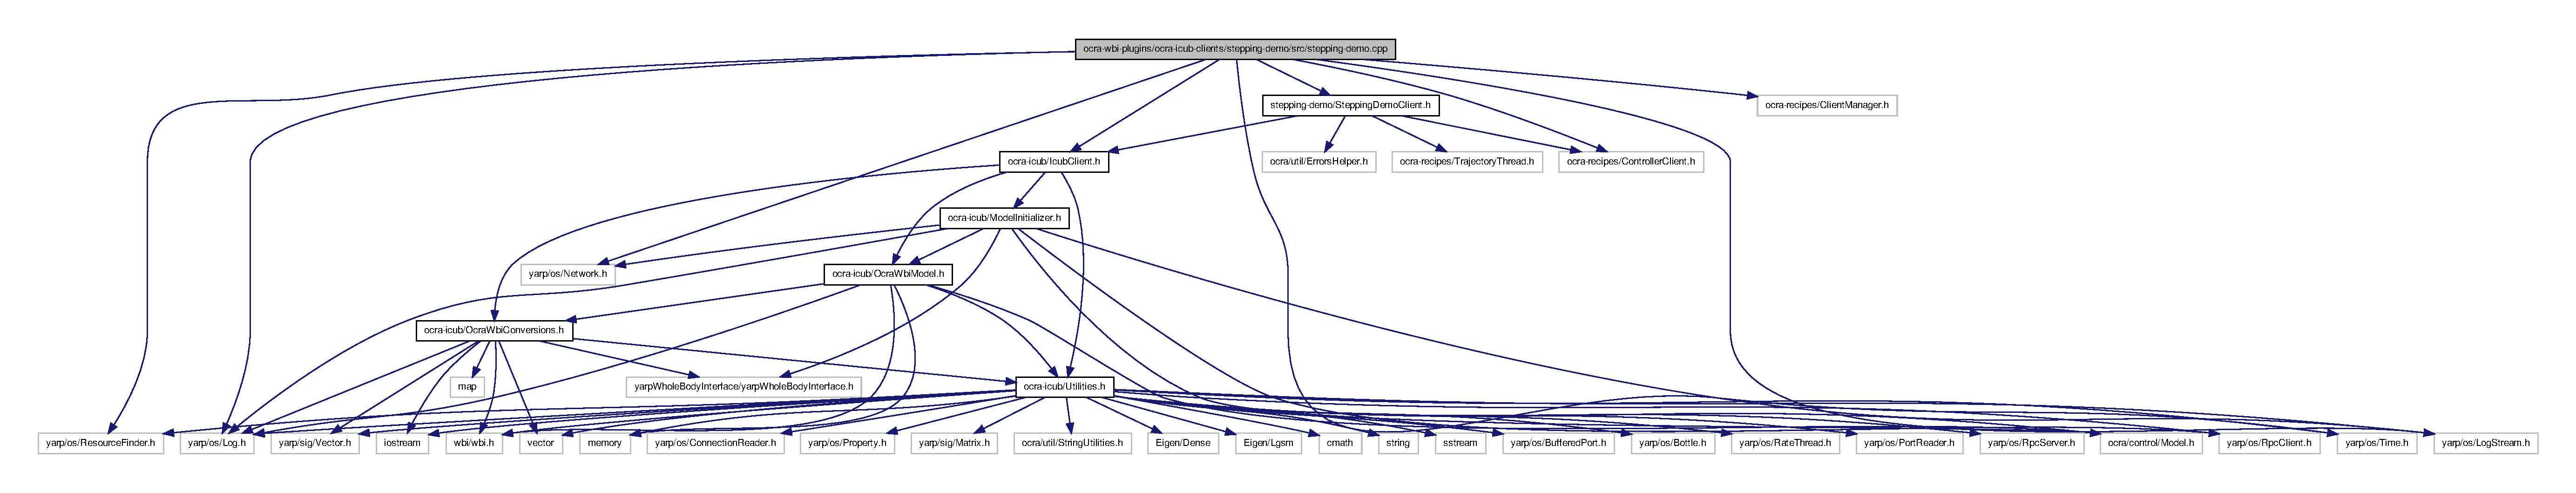
\includegraphics[width=350pt]{stepping-demo_8cpp__incl}
\end{center}
\end{figure}
\subsection*{\-Functions}
\begin{DoxyCompactItemize}
\item 
int \hyperlink{stepping-demo_8cpp_a0ddf1224851353fc92bfbff6f499fa97}{main} (int argc, char $\ast$argv\mbox{[}$\,$\mbox{]})
\end{DoxyCompactItemize}


\subsection{\-Detailed \-Description}
\begin{DoxyAuthor}{\-Author}
\mbox{[}\-Ryan \-Lober\mbox{]}(\href{http://www.ryanlober.com}{\tt http\-://www.\-ryanlober.\-com}) 

\mbox{[}\-Antoine \-Hoarau\mbox{]}(\href{http://ahoarau.github.io}{\tt http\-://ahoarau.\-github.\-io}) 

\mbox{[}\-Jorhabib \-Eljaik\mbox{]}(\href{https://github.com/jeljaik}{\tt https\-://github.\-com/jeljaik}) 
\end{DoxyAuthor}
\begin{DoxyDate}{\-Date}
\-Feb 2016 
\end{DoxyDate}
\begin{DoxyCopyright}{\-Copyright}
\-G\-N\-U \-General \-Public \-License. 
\end{DoxyCopyright}


\subsection{\-Function \-Documentation}
\hypertarget{stepping-demo_8cpp_a0ddf1224851353fc92bfbff6f499fa97}{\index{stepping-\/demo.\-cpp@{stepping-\/demo.\-cpp}!main@{main}}
\index{main@{main}!stepping-demo.cpp@{stepping-\/demo.\-cpp}}
\subsubsection[{main}]{\setlength{\rightskip}{0pt plus 5cm}int {\bf main} (
\begin{DoxyParamCaption}
\item[{int}]{argc, }
\item[{char $\ast$}]{argv\mbox{[}$\,$\mbox{]}}
\end{DoxyParamCaption}
)}}\label{stepping-demo_8cpp_a0ddf1224851353fc92bfbff6f499fa97}

\hypertarget{SteppingDemoClient_8cpp}{\section{ocra-\/wbi-\/plugins/ocra-\/icub-\/clients/stepping-\/demo/src/\-Stepping\-Demo\-Client.cpp \-File \-Reference}
\label{SteppingDemoClient_8cpp}\index{ocra-\/wbi-\/plugins/ocra-\/icub-\/clients/stepping-\/demo/src/\-Stepping\-Demo\-Client.\-cpp@{ocra-\/wbi-\/plugins/ocra-\/icub-\/clients/stepping-\/demo/src/\-Stepping\-Demo\-Client.\-cpp}}
}
{\ttfamily \#include \char`\"{}stepping-\/demo/\-Stepping\-Demo\-Client.\-h\char`\"{}}\*
\-Include dependency graph for \-Stepping\-Demo\-Client.\-cpp\-:\nopagebreak
\begin{figure}[H]
\begin{center}
\leavevmode
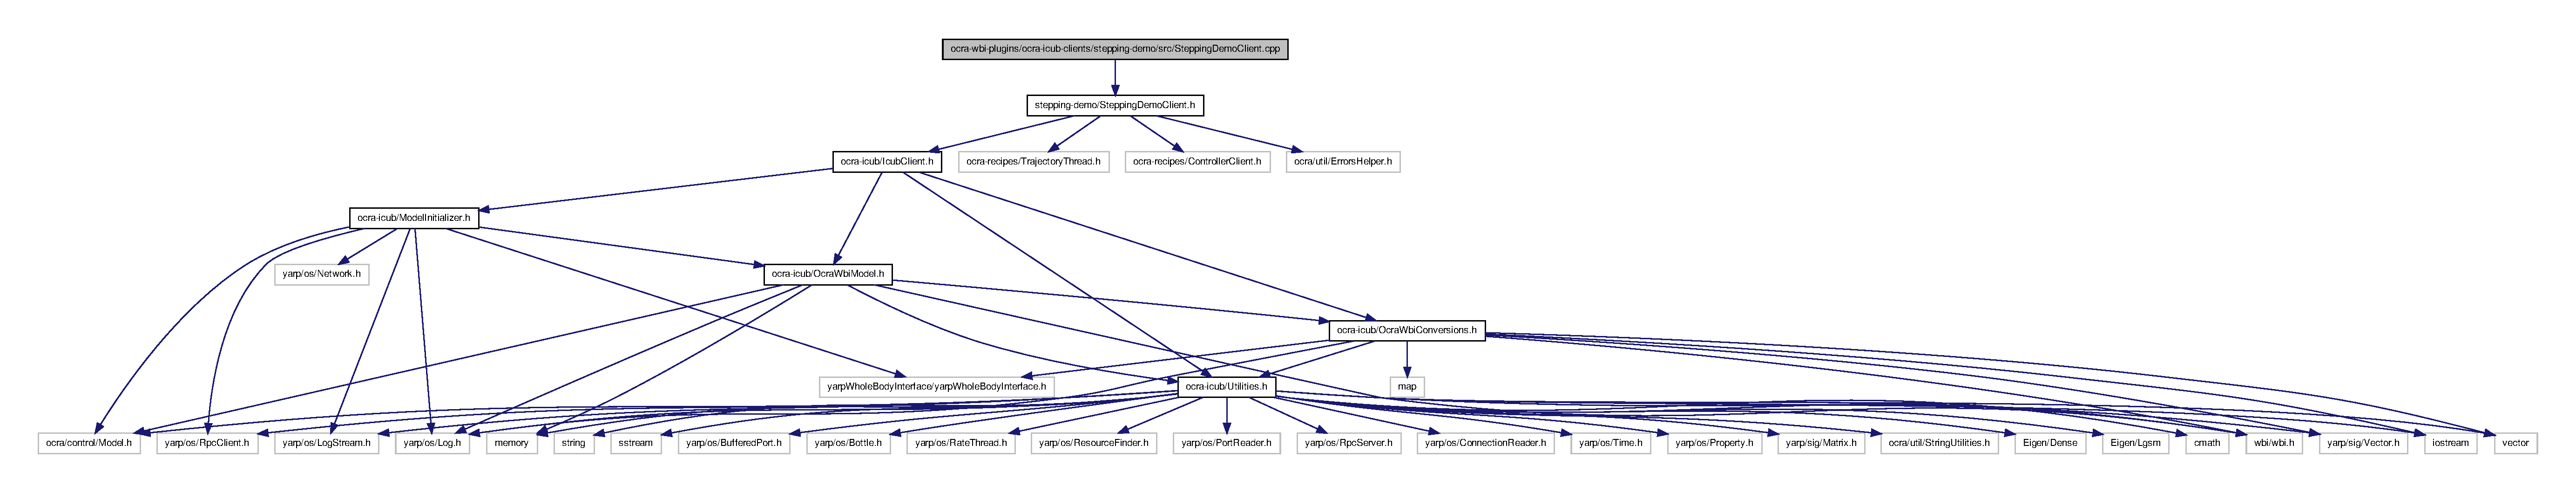
\includegraphics[width=350pt]{SteppingDemoClient_8cpp__incl}
\end{center}
\end{figure}

\hypertarget{TaskOpsClient_8h}{\section{ocra-\/wbi-\/plugins/ocra-\/icub-\/clients/task-\/operations-\/demo/include/task-\/operations-\/demo/\-Task\-Ops\-Client.h \-File \-Reference}
\label{TaskOpsClient_8h}\index{ocra-\/wbi-\/plugins/ocra-\/icub-\/clients/task-\/operations-\/demo/include/task-\/operations-\/demo/\-Task\-Ops\-Client.\-h@{ocra-\/wbi-\/plugins/ocra-\/icub-\/clients/task-\/operations-\/demo/include/task-\/operations-\/demo/\-Task\-Ops\-Client.\-h}}
}
{\ttfamily \#include $<$ocra-\/icub/\-Icub\-Client.\-h$>$}\*
{\ttfamily \#include $<$ocra-\/recipes/\-Trajectory\-Thread.\-h$>$}\*
{\ttfamily \#include $<$ocra-\/recipes/\-Controller\-Client.\-h$>$}\*
\-Include dependency graph for \-Task\-Ops\-Client.\-h\-:\nopagebreak
\begin{figure}[H]
\begin{center}
\leavevmode
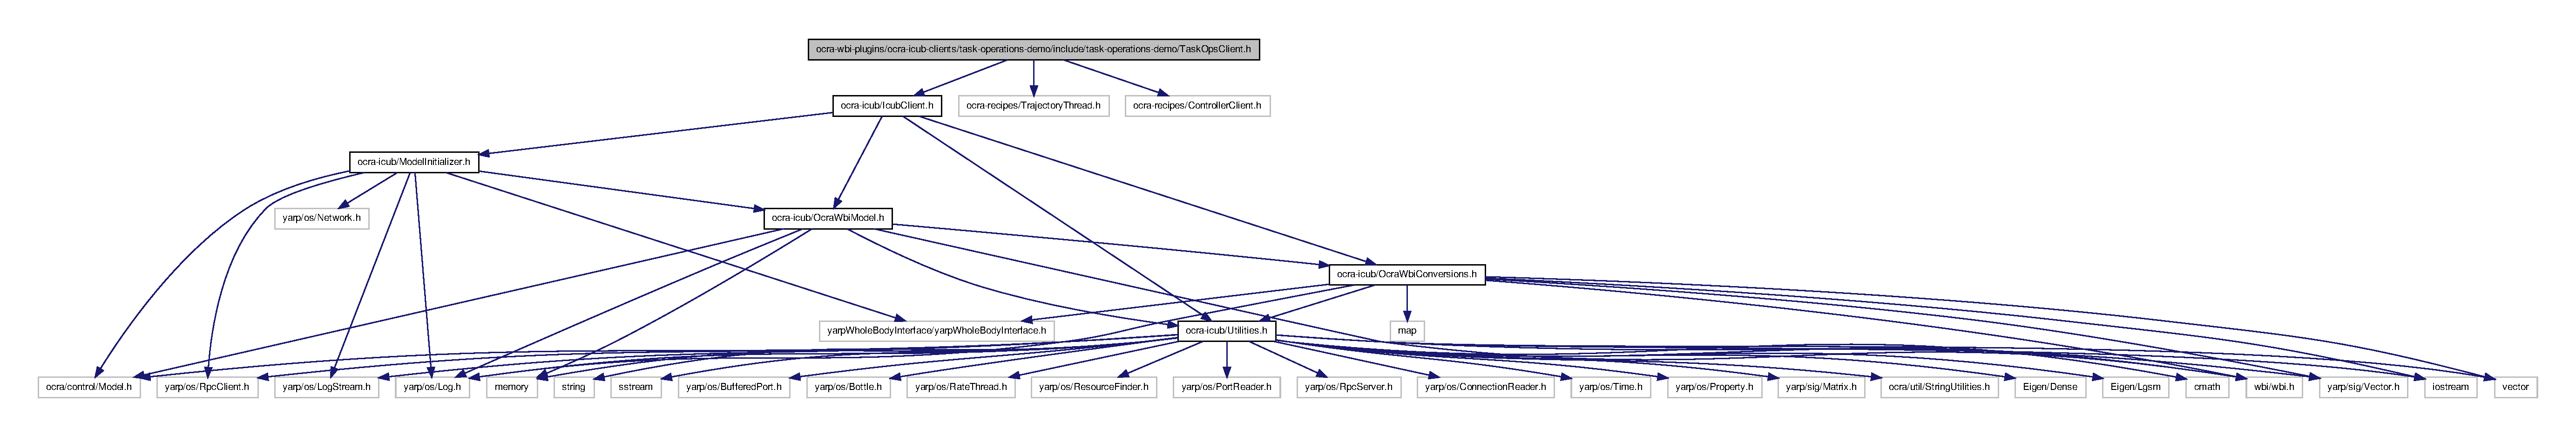
\includegraphics[width=350pt]{TaskOpsClient_8h__incl}
\end{center}
\end{figure}
\-This graph shows which files directly or indirectly include this file\-:\nopagebreak
\begin{figure}[H]
\begin{center}
\leavevmode
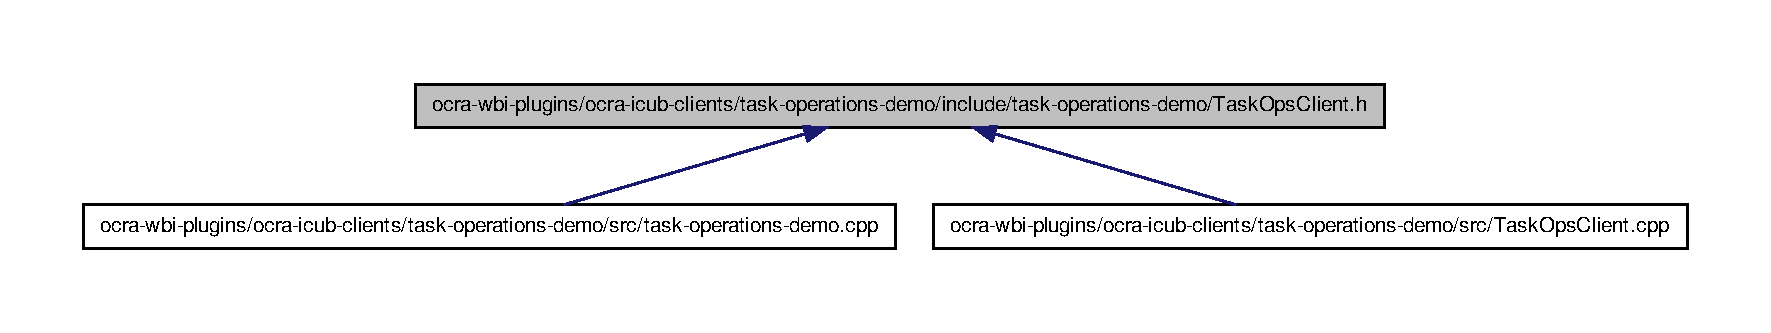
\includegraphics[width=350pt]{TaskOpsClient_8h__dep__incl}
\end{center}
\end{figure}
\subsection*{\-Classes}
\begin{DoxyCompactItemize}
\item 
class \hyperlink{classTaskOpsClient}{\-Task\-Ops\-Client}
\end{DoxyCompactItemize}
\subsection*{\-Enumerations}
\begin{DoxyCompactItemize}
\item 
enum \hyperlink{TaskOpsClient_8h_a0140057ae3fbe1db5f5c418dfc67d9db}{\-T\-H\-I\-N\-G\-S\-\_\-\-T\-O\-\_\-\-D\-O} \{ \*
\hyperlink{TaskOpsClient_8h_a0140057ae3fbe1db5f5c418dfc67d9dbaf831abed77e2c76cacc256b8b16f2b2a}{\-R\-E\-M\-O\-V\-E\-\_\-\-T\-A\-S\-K}, 
\hyperlink{TaskOpsClient_8h_a0140057ae3fbe1db5f5c418dfc67d9dba6aa666a68fed72da5438e0ef9b7cba8f}{\-A\-D\-D\-\_\-\-N\-E\-W\-\_\-\-T\-A\-S\-K}, 
\hyperlink{TaskOpsClient_8h_a0140057ae3fbe1db5f5c418dfc67d9dba8ffc9eba853106ab798ee2a0c5763d1b}{\-A\-D\-D\-\_\-\-E\-X\-I\-S\-T\-I\-N\-G\-\_\-\-T\-A\-S\-K}, 
\hyperlink{TaskOpsClient_8h_a0140057ae3fbe1db5f5c418dfc67d9dba7eaf30861bc723f003ea1a8e4a7a4977}{\-A\-D\-D\-\_\-\-E\-X\-I\-S\-T\-I\-N\-G\-\_\-\-T\-A\-S\-K\-\_\-\-N\-O\-\_\-\-O\-V\-E\-R\-W\-R\-I\-T\-E}, 
\*
\hyperlink{TaskOpsClient_8h_a0140057ae3fbe1db5f5c418dfc67d9dbacfe24a7b308a82835c8a9a9a89bc4ca2}{\-N\-O\-T\-H\-I\-N\-G}
 \}
\end{DoxyCompactItemize}


\subsection{\-Enumeration \-Type \-Documentation}
\hypertarget{TaskOpsClient_8h_a0140057ae3fbe1db5f5c418dfc67d9db}{\index{\-Task\-Ops\-Client.\-h@{\-Task\-Ops\-Client.\-h}!\-T\-H\-I\-N\-G\-S\-\_\-\-T\-O\-\_\-\-D\-O@{\-T\-H\-I\-N\-G\-S\-\_\-\-T\-O\-\_\-\-D\-O}}
\index{\-T\-H\-I\-N\-G\-S\-\_\-\-T\-O\-\_\-\-D\-O@{\-T\-H\-I\-N\-G\-S\-\_\-\-T\-O\-\_\-\-D\-O}!TaskOpsClient.h@{\-Task\-Ops\-Client.\-h}}
\subsubsection[{\-T\-H\-I\-N\-G\-S\-\_\-\-T\-O\-\_\-\-D\-O}]{\setlength{\rightskip}{0pt plus 5cm}enum {\bf \-T\-H\-I\-N\-G\-S\-\_\-\-T\-O\-\_\-\-D\-O}}}\label{TaskOpsClient_8h_a0140057ae3fbe1db5f5c418dfc67d9db}
\begin{Desc}
\item[\-Enumerator\-: ]\par
\begin{description}
\index{\-R\-E\-M\-O\-V\-E\-\_\-\-T\-A\-S\-K@{\-R\-E\-M\-O\-V\-E\-\_\-\-T\-A\-S\-K}!\-Task\-Ops\-Client.\-h@{\-Task\-Ops\-Client.\-h}}\index{\-Task\-Ops\-Client.\-h@{\-Task\-Ops\-Client.\-h}!\-R\-E\-M\-O\-V\-E\-\_\-\-T\-A\-S\-K@{\-R\-E\-M\-O\-V\-E\-\_\-\-T\-A\-S\-K}}\item[{\em 
\hypertarget{TaskOpsClient_8h_a0140057ae3fbe1db5f5c418dfc67d9dbaf831abed77e2c76cacc256b8b16f2b2a}{\-R\-E\-M\-O\-V\-E\-\_\-\-T\-A\-S\-K}\label{TaskOpsClient_8h_a0140057ae3fbe1db5f5c418dfc67d9dbaf831abed77e2c76cacc256b8b16f2b2a}
}]\index{\-A\-D\-D\-\_\-\-N\-E\-W\-\_\-\-T\-A\-S\-K@{\-A\-D\-D\-\_\-\-N\-E\-W\-\_\-\-T\-A\-S\-K}!\-Task\-Ops\-Client.\-h@{\-Task\-Ops\-Client.\-h}}\index{\-Task\-Ops\-Client.\-h@{\-Task\-Ops\-Client.\-h}!\-A\-D\-D\-\_\-\-N\-E\-W\-\_\-\-T\-A\-S\-K@{\-A\-D\-D\-\_\-\-N\-E\-W\-\_\-\-T\-A\-S\-K}}\item[{\em 
\hypertarget{TaskOpsClient_8h_a0140057ae3fbe1db5f5c418dfc67d9dba6aa666a68fed72da5438e0ef9b7cba8f}{\-A\-D\-D\-\_\-\-N\-E\-W\-\_\-\-T\-A\-S\-K}\label{TaskOpsClient_8h_a0140057ae3fbe1db5f5c418dfc67d9dba6aa666a68fed72da5438e0ef9b7cba8f}
}]\index{\-A\-D\-D\-\_\-\-E\-X\-I\-S\-T\-I\-N\-G\-\_\-\-T\-A\-S\-K@{\-A\-D\-D\-\_\-\-E\-X\-I\-S\-T\-I\-N\-G\-\_\-\-T\-A\-S\-K}!\-Task\-Ops\-Client.\-h@{\-Task\-Ops\-Client.\-h}}\index{\-Task\-Ops\-Client.\-h@{\-Task\-Ops\-Client.\-h}!\-A\-D\-D\-\_\-\-E\-X\-I\-S\-T\-I\-N\-G\-\_\-\-T\-A\-S\-K@{\-A\-D\-D\-\_\-\-E\-X\-I\-S\-T\-I\-N\-G\-\_\-\-T\-A\-S\-K}}\item[{\em 
\hypertarget{TaskOpsClient_8h_a0140057ae3fbe1db5f5c418dfc67d9dba8ffc9eba853106ab798ee2a0c5763d1b}{\-A\-D\-D\-\_\-\-E\-X\-I\-S\-T\-I\-N\-G\-\_\-\-T\-A\-S\-K}\label{TaskOpsClient_8h_a0140057ae3fbe1db5f5c418dfc67d9dba8ffc9eba853106ab798ee2a0c5763d1b}
}]\index{\-A\-D\-D\-\_\-\-E\-X\-I\-S\-T\-I\-N\-G\-\_\-\-T\-A\-S\-K\-\_\-\-N\-O\-\_\-\-O\-V\-E\-R\-W\-R\-I\-T\-E@{\-A\-D\-D\-\_\-\-E\-X\-I\-S\-T\-I\-N\-G\-\_\-\-T\-A\-S\-K\-\_\-\-N\-O\-\_\-\-O\-V\-E\-R\-W\-R\-I\-T\-E}!\-Task\-Ops\-Client.\-h@{\-Task\-Ops\-Client.\-h}}\index{\-Task\-Ops\-Client.\-h@{\-Task\-Ops\-Client.\-h}!\-A\-D\-D\-\_\-\-E\-X\-I\-S\-T\-I\-N\-G\-\_\-\-T\-A\-S\-K\-\_\-\-N\-O\-\_\-\-O\-V\-E\-R\-W\-R\-I\-T\-E@{\-A\-D\-D\-\_\-\-E\-X\-I\-S\-T\-I\-N\-G\-\_\-\-T\-A\-S\-K\-\_\-\-N\-O\-\_\-\-O\-V\-E\-R\-W\-R\-I\-T\-E}}\item[{\em 
\hypertarget{TaskOpsClient_8h_a0140057ae3fbe1db5f5c418dfc67d9dba7eaf30861bc723f003ea1a8e4a7a4977}{\-A\-D\-D\-\_\-\-E\-X\-I\-S\-T\-I\-N\-G\-\_\-\-T\-A\-S\-K\-\_\-\-N\-O\-\_\-\-O\-V\-E\-R\-W\-R\-I\-T\-E}\label{TaskOpsClient_8h_a0140057ae3fbe1db5f5c418dfc67d9dba7eaf30861bc723f003ea1a8e4a7a4977}
}]\index{\-N\-O\-T\-H\-I\-N\-G@{\-N\-O\-T\-H\-I\-N\-G}!\-Task\-Ops\-Client.\-h@{\-Task\-Ops\-Client.\-h}}\index{\-Task\-Ops\-Client.\-h@{\-Task\-Ops\-Client.\-h}!\-N\-O\-T\-H\-I\-N\-G@{\-N\-O\-T\-H\-I\-N\-G}}\item[{\em 
\hypertarget{TaskOpsClient_8h_a0140057ae3fbe1db5f5c418dfc67d9dbacfe24a7b308a82835c8a9a9a89bc4ca2}{\-N\-O\-T\-H\-I\-N\-G}\label{TaskOpsClient_8h_a0140057ae3fbe1db5f5c418dfc67d9dbacfe24a7b308a82835c8a9a9a89bc4ca2}
}]\end{description}
\end{Desc}


\hypertarget{task-operations-demo_8cpp}{\section{ocra-\/wbi-\/plugins/ocra-\/icub-\/clients/task-\/operations-\/demo/src/task-\/operations-\/demo.cpp \-File \-Reference}
\label{task-operations-demo_8cpp}\index{ocra-\/wbi-\/plugins/ocra-\/icub-\/clients/task-\/operations-\/demo/src/task-\/operations-\/demo.\-cpp@{ocra-\/wbi-\/plugins/ocra-\/icub-\/clients/task-\/operations-\/demo/src/task-\/operations-\/demo.\-cpp}}
}
{\ttfamily \#include $<$yarp/os/\-Resource\-Finder.\-h$>$}\*
{\ttfamily \#include $<$yarp/os/\-Network.\-h$>$}\*
{\ttfamily \#include $<$yarp/os/\-Log.\-h$>$}\*
{\ttfamily \#include $<$yarp/os/\-Log\-Stream.\-h$>$}\*
{\ttfamily \#include $<$yarp/os/\-Time.\-h$>$}\*
{\ttfamily \#include \char`\"{}task-\/operations-\/demo/\-Task\-Ops\-Client.\-h\char`\"{}}\*
{\ttfamily \#include $<$ocra-\/icub/\-Icub\-Client.\-h$>$}\*
{\ttfamily \#include $<$ocra-\/recipes/\-Controller\-Client.\-h$>$}\*
{\ttfamily \#include $<$ocra-\/recipes/\-Client\-Manager.\-h$>$}\*
\-Include dependency graph for task-\/operations-\/demo.cpp\-:
\nopagebreak
\begin{figure}[H]
\begin{center}
\leavevmode
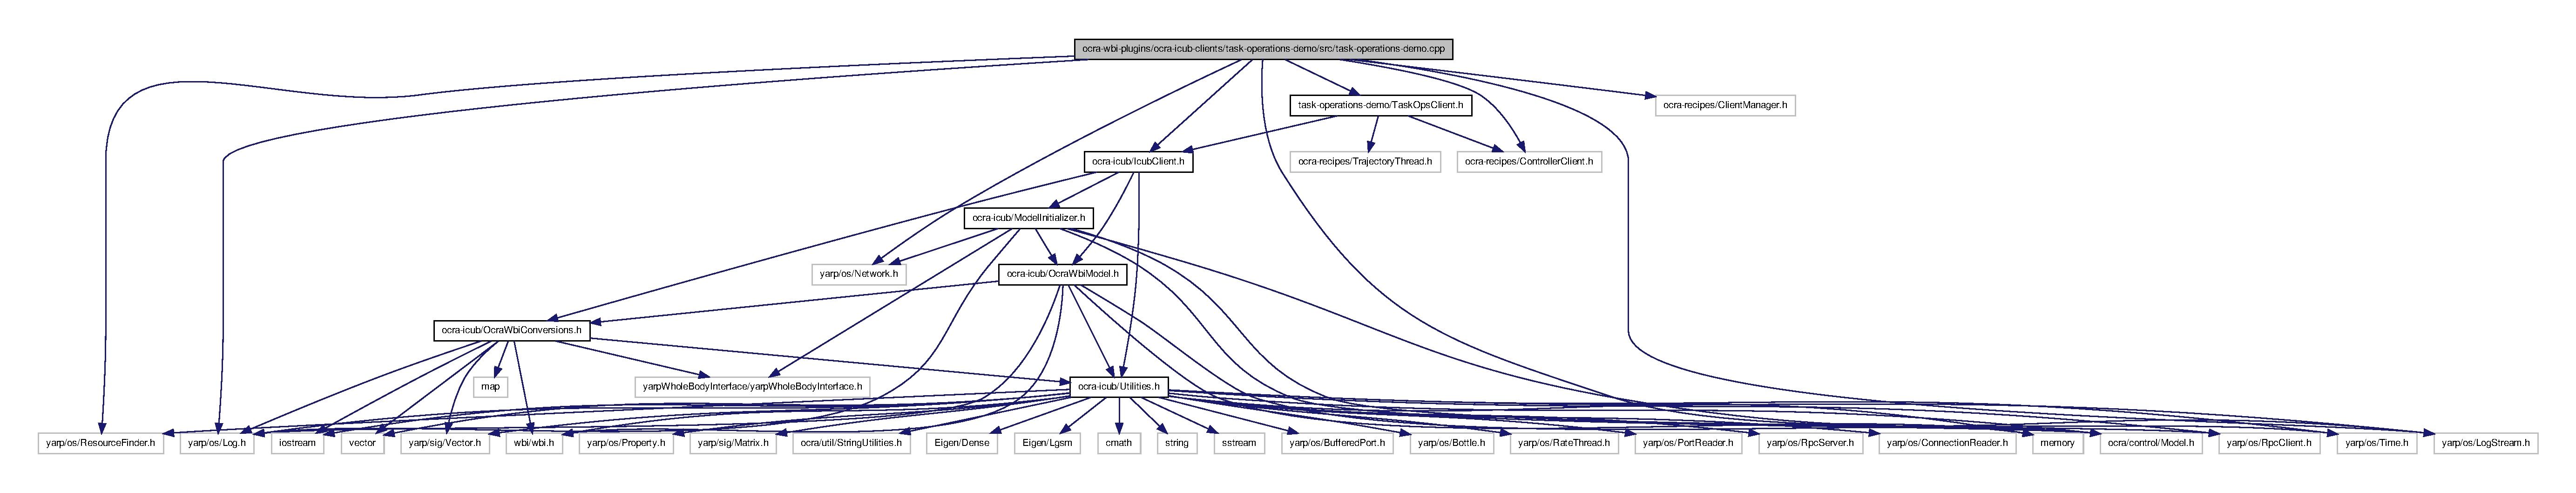
\includegraphics[width=350pt]{task-operations-demo_8cpp__incl}
\end{center}
\end{figure}
\subsection*{\-Functions}
\begin{DoxyCompactItemize}
\item 
int \hyperlink{task-operations-demo_8cpp_a0ddf1224851353fc92bfbff6f499fa97}{main} (int argc, char $\ast$argv\mbox{[}$\,$\mbox{]})
\end{DoxyCompactItemize}


\subsection{\-Function \-Documentation}
\hypertarget{task-operations-demo_8cpp_a0ddf1224851353fc92bfbff6f499fa97}{\index{task-\/operations-\/demo.\-cpp@{task-\/operations-\/demo.\-cpp}!main@{main}}
\index{main@{main}!task-operations-demo.cpp@{task-\/operations-\/demo.\-cpp}}
\subsubsection[{main}]{\setlength{\rightskip}{0pt plus 5cm}int {\bf main} (
\begin{DoxyParamCaption}
\item[{int}]{argc, }
\item[{char $\ast$}]{argv\mbox{[}$\,$\mbox{]}}
\end{DoxyParamCaption}
)}}\label{task-operations-demo_8cpp_a0ddf1224851353fc92bfbff6f499fa97}

\hypertarget{TaskOpsClient_8cpp}{\section{ocra-\/wbi-\/plugins/ocra-\/icub-\/clients/task-\/operations-\/demo/src/\-Task\-Ops\-Client.cpp \-File \-Reference}
\label{TaskOpsClient_8cpp}\index{ocra-\/wbi-\/plugins/ocra-\/icub-\/clients/task-\/operations-\/demo/src/\-Task\-Ops\-Client.\-cpp@{ocra-\/wbi-\/plugins/ocra-\/icub-\/clients/task-\/operations-\/demo/src/\-Task\-Ops\-Client.\-cpp}}
}
{\ttfamily \#include \char`\"{}task-\/operations-\/demo/\-Task\-Ops\-Client.\-h\char`\"{}}\*
\-Include dependency graph for \-Task\-Ops\-Client.\-cpp\-:
\nopagebreak
\begin{figure}[H]
\begin{center}
\leavevmode
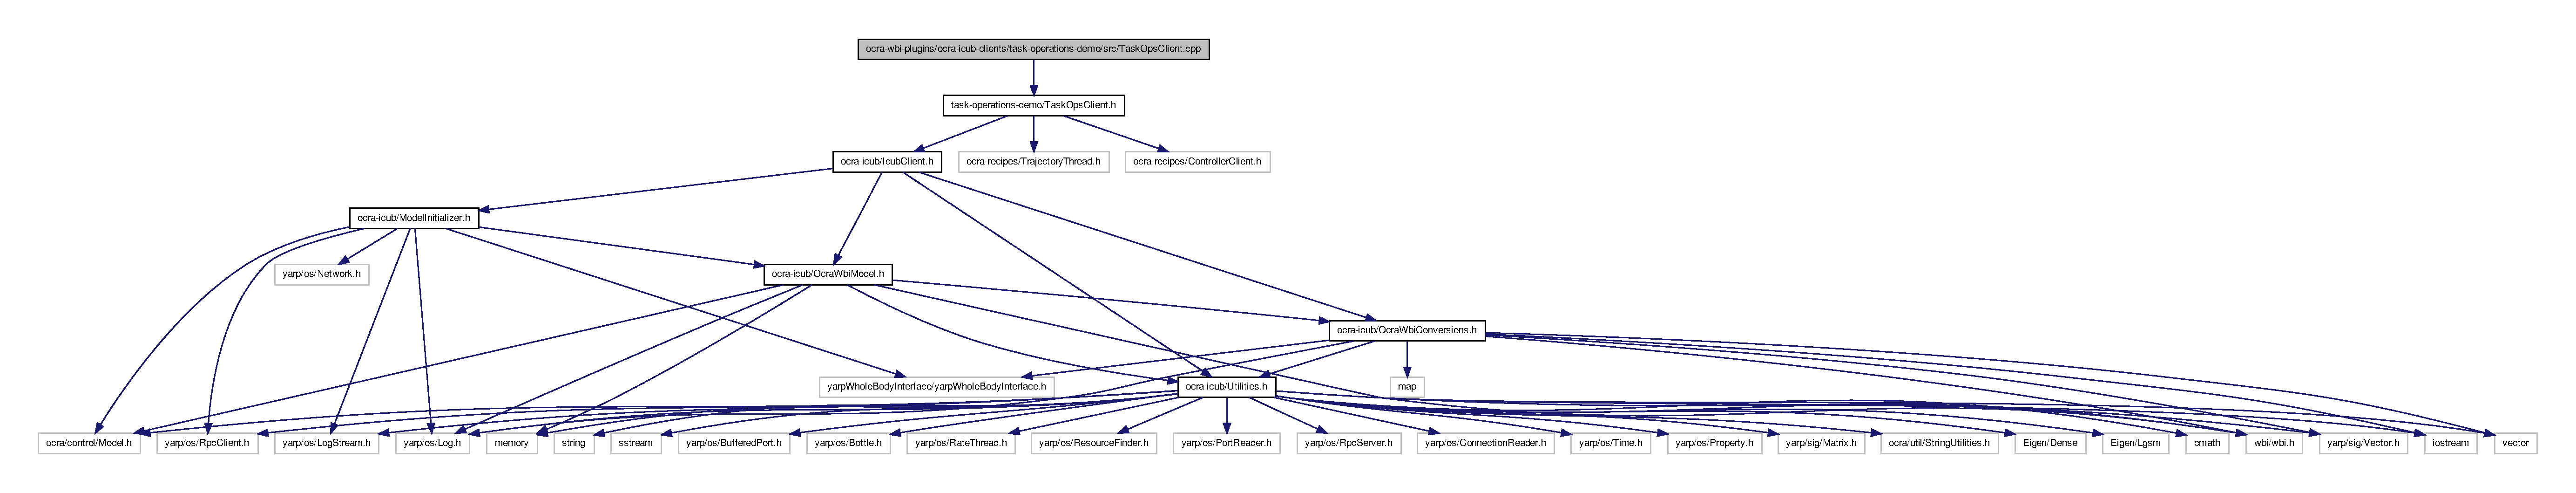
\includegraphics[width=350pt]{TaskOpsClient_8cpp__incl}
\end{center}
\end{figure}

\hypertarget{BaseOfSupport_8h}{\section{ocra-\/wbi-\/plugins/ocra-\/icub-\/clients/walking-\/client/include/walking-\/client/\-Base\-Of\-Support.h \-File \-Reference}
\label{BaseOfSupport_8h}\index{ocra-\/wbi-\/plugins/ocra-\/icub-\/clients/walking-\/client/include/walking-\/client/\-Base\-Of\-Support.\-h@{ocra-\/wbi-\/plugins/ocra-\/icub-\/clients/walking-\/client/include/walking-\/client/\-Base\-Of\-Support.\-h}}
}
{\ttfamily \#include $<$boost/geometry.\-hpp$>$}\*
{\ttfamily \#include $<$boost/geometry/geometries/polygon.\-hpp$>$}\*
{\ttfamily \#include $<$boost/geometry/geometries/box.\-hpp$>$}\*
{\ttfamily \#include $<$boost/geometry/geometries/adapted/boost\-\_\-tuple.\-hpp$>$}\*
{\ttfamily \#include \char`\"{}unsupported/\-Eigen/\-Matrix\-Functions\char`\"{}}\*
{\ttfamily \#include $<$\-Eigen/\-Core$>$}\*
{\ttfamily \#include $<$walking-\/client/\-M\-I\-Q\-P\-State.\-h$>$}\*
{\ttfamily \#include $<$walking-\/client/\-Step\-Controller.\-h$>$}\*
{\ttfamily \#include $<$walking-\/client/utils.\-h$>$}\*
{\ttfamily \#include $<$ocra-\/recipes/\-Task\-Connection.\-h$>$}\*
\-Include dependency graph for \-Base\-Of\-Support.\-h\-:\nopagebreak
\begin{figure}[H]
\begin{center}
\leavevmode
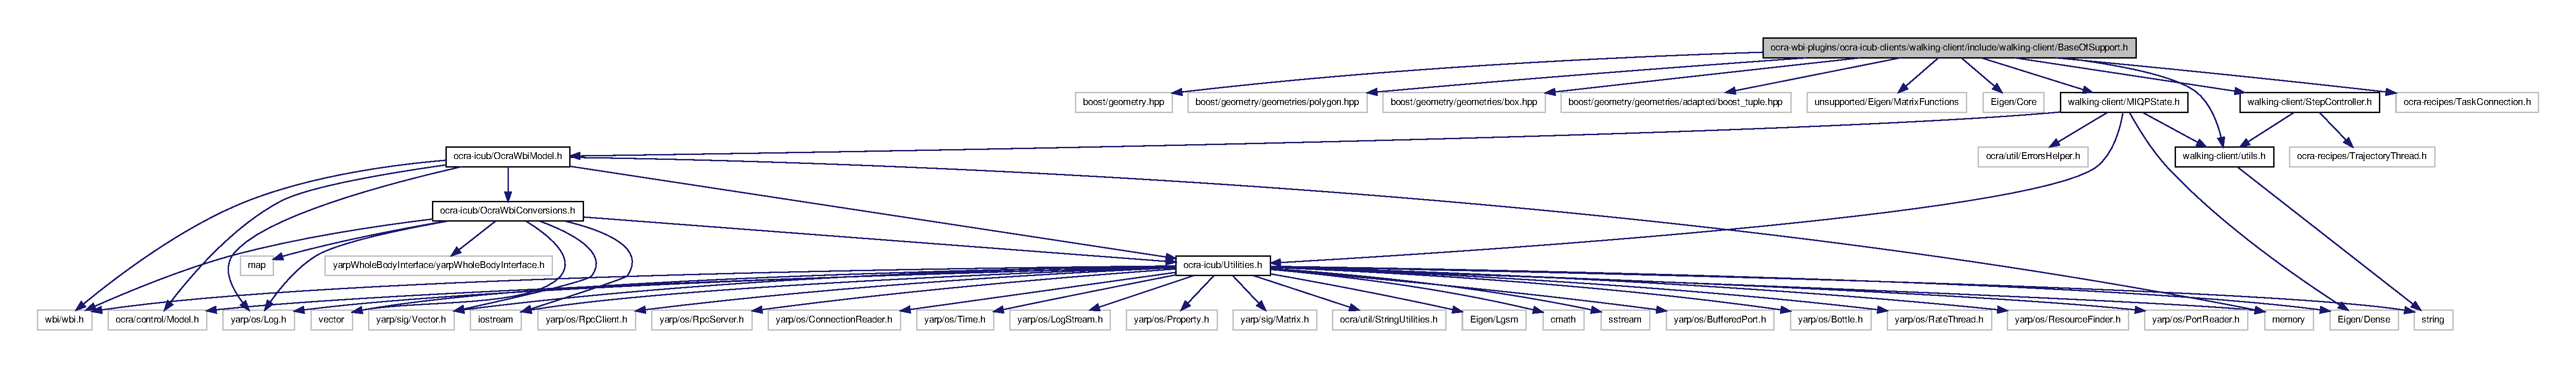
\includegraphics[width=350pt]{BaseOfSupport_8h__incl}
\end{center}
\end{figure}
\-This graph shows which files directly or indirectly include this file\-:\nopagebreak
\begin{figure}[H]
\begin{center}
\leavevmode
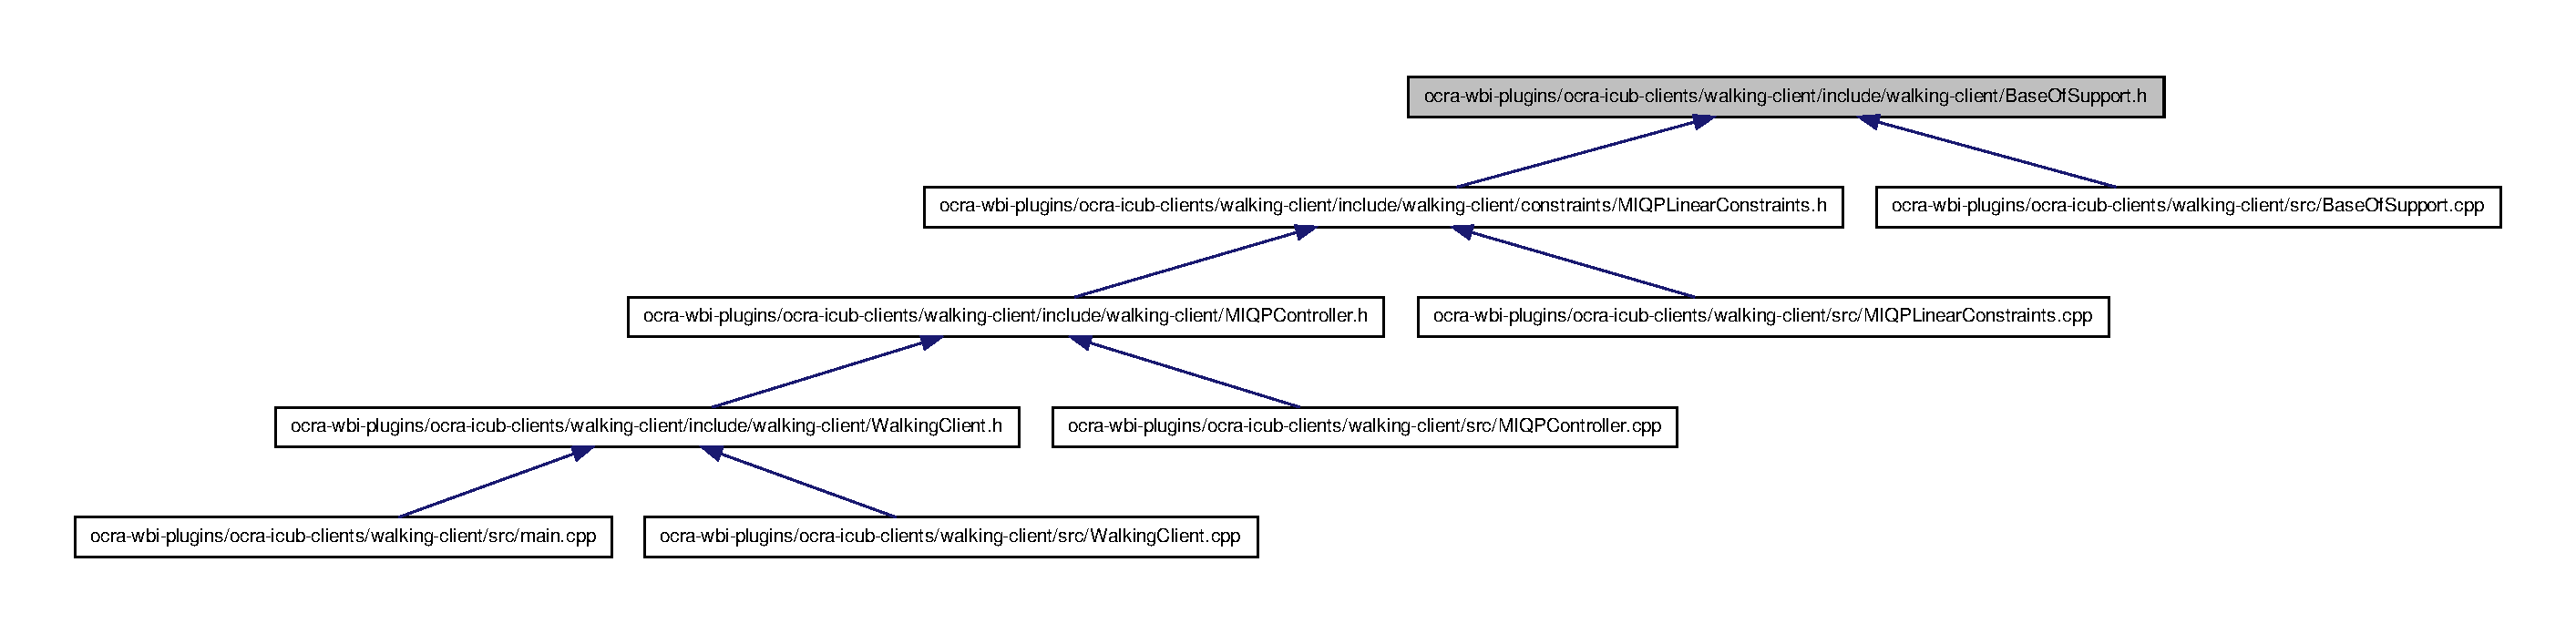
\includegraphics[width=350pt]{BaseOfSupport_8h__dep__incl}
\end{center}
\end{figure}
\subsection*{\-Classes}
\begin{DoxyCompactItemize}
\item 
class \hyperlink{classBaseOfSupport}{\-Base\-Of\-Support}
\begin{DoxyCompactList}\small\item\em \-Builds base of support and corresponding constraints based on the robot's feet location. \end{DoxyCompactList}\end{DoxyCompactItemize}
\subsection*{\-Typedefs}
\begin{DoxyCompactItemize}
\item 
typedef boost\-::tuple$<$ double, \*
double $>$ \hyperlink{BaseOfSupport_8h_ac09614442423c31cf4372f1304b03cb0}{point}
\item 
typedef \*
boost\-::geometry\-::model\-::polygon\*
$<$ \hyperlink{BaseOfSupport_8h_ac09614442423c31cf4372f1304b03cb0}{point} $>$ \hyperlink{BaseOfSupport_8h_a3b0bf53b9d321e300a59729ebe10e02c}{\-Polygon}
\item 
typedef \*
boost\-::geometry\-::model\-::box\*
$<$ \hyperlink{BaseOfSupport_8h_ac09614442423c31cf4372f1304b03cb0}{point} $>$ \hyperlink{BaseOfSupport_8h_ac470b50f15f04405e67b9031615134f0}{\-Box}
\end{DoxyCompactItemize}


\subsection{\-Typedef \-Documentation}
\hypertarget{BaseOfSupport_8h_ac470b50f15f04405e67b9031615134f0}{\index{\-Base\-Of\-Support.\-h@{\-Base\-Of\-Support.\-h}!\-Box@{\-Box}}
\index{\-Box@{\-Box}!BaseOfSupport.h@{\-Base\-Of\-Support.\-h}}
\subsubsection[{\-Box}]{\setlength{\rightskip}{0pt plus 5cm}typedef boost\-::geometry\-::model\-::box$<${\bf point}$>$ {\bf \-Box}}}\label{BaseOfSupport_8h_ac470b50f15f04405e67b9031615134f0}
\hypertarget{BaseOfSupport_8h_ac09614442423c31cf4372f1304b03cb0}{\index{\-Base\-Of\-Support.\-h@{\-Base\-Of\-Support.\-h}!point@{point}}
\index{point@{point}!BaseOfSupport.h@{\-Base\-Of\-Support.\-h}}
\subsubsection[{point}]{\setlength{\rightskip}{0pt plus 5cm}typedef boost\-::tuple$<$double, double$>$ {\bf point}}}\label{BaseOfSupport_8h_ac09614442423c31cf4372f1304b03cb0}
\hypertarget{BaseOfSupport_8h_a3b0bf53b9d321e300a59729ebe10e02c}{\index{\-Base\-Of\-Support.\-h@{\-Base\-Of\-Support.\-h}!\-Polygon@{\-Polygon}}
\index{\-Polygon@{\-Polygon}!BaseOfSupport.h@{\-Base\-Of\-Support.\-h}}
\subsubsection[{\-Polygon}]{\setlength{\rightskip}{0pt plus 5cm}typedef boost\-::geometry\-::model\-::polygon$<${\bf point}$>$ {\bf \-Polygon}}}\label{BaseOfSupport_8h_a3b0bf53b9d321e300a59729ebe10e02c}

\hypertarget{AdmissibilityConstraints_8h}{\section{ocra-\/wbi-\/plugins/ocra-\/icub-\/clients/walking-\/client/include/walking-\/client/constraints/\-Admissibility\-Constraints.h \-File \-Reference}
\label{AdmissibilityConstraints_8h}\index{ocra-\/wbi-\/plugins/ocra-\/icub-\/clients/walking-\/client/include/walking-\/client/constraints/\-Admissibility\-Constraints.\-h@{ocra-\/wbi-\/plugins/ocra-\/icub-\/clients/walking-\/client/include/walking-\/client/constraints/\-Admissibility\-Constraints.\-h}}
}
{\ttfamily \#include \char`\"{}walking-\/client/constraints/\-Constraint.\-h\char`\"{}}\*
{\ttfamily \#include \char`\"{}walking-\/client/constraints/\-S\-S\-D\-S\-Alternation.\-h\char`\"{}}\*
{\ttfamily \#include \char`\"{}walking-\/client/constraints/\-Single\-Support.\-h\char`\"{}}\*
{\ttfamily \#include \char`\"{}walking-\/client/constraints/\-Contact\-Config\-History.\-h\char`\"{}}\*
{\ttfamily \#include \char`\"{}walking-\/client/constraints/\-Contact\-Config\-Enforcement.\-h\char`\"{}}\*
\-Include dependency graph for \-Admissibility\-Constraints.\-h\-:
\nopagebreak
\begin{figure}[H]
\begin{center}
\leavevmode
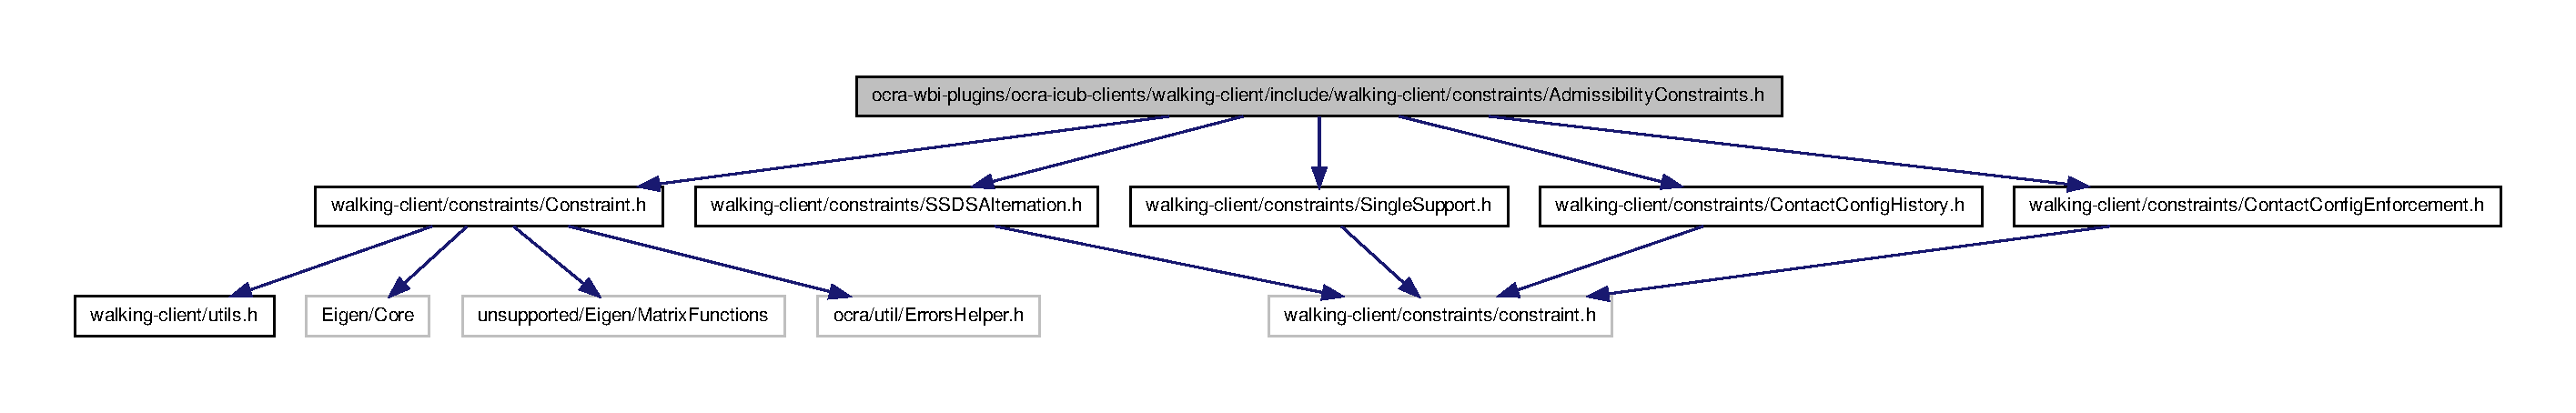
\includegraphics[width=350pt]{AdmissibilityConstraints_8h__incl}
\end{center}
\end{figure}
\-This graph shows which files directly or indirectly include this file\-:\nopagebreak
\begin{figure}[H]
\begin{center}
\leavevmode
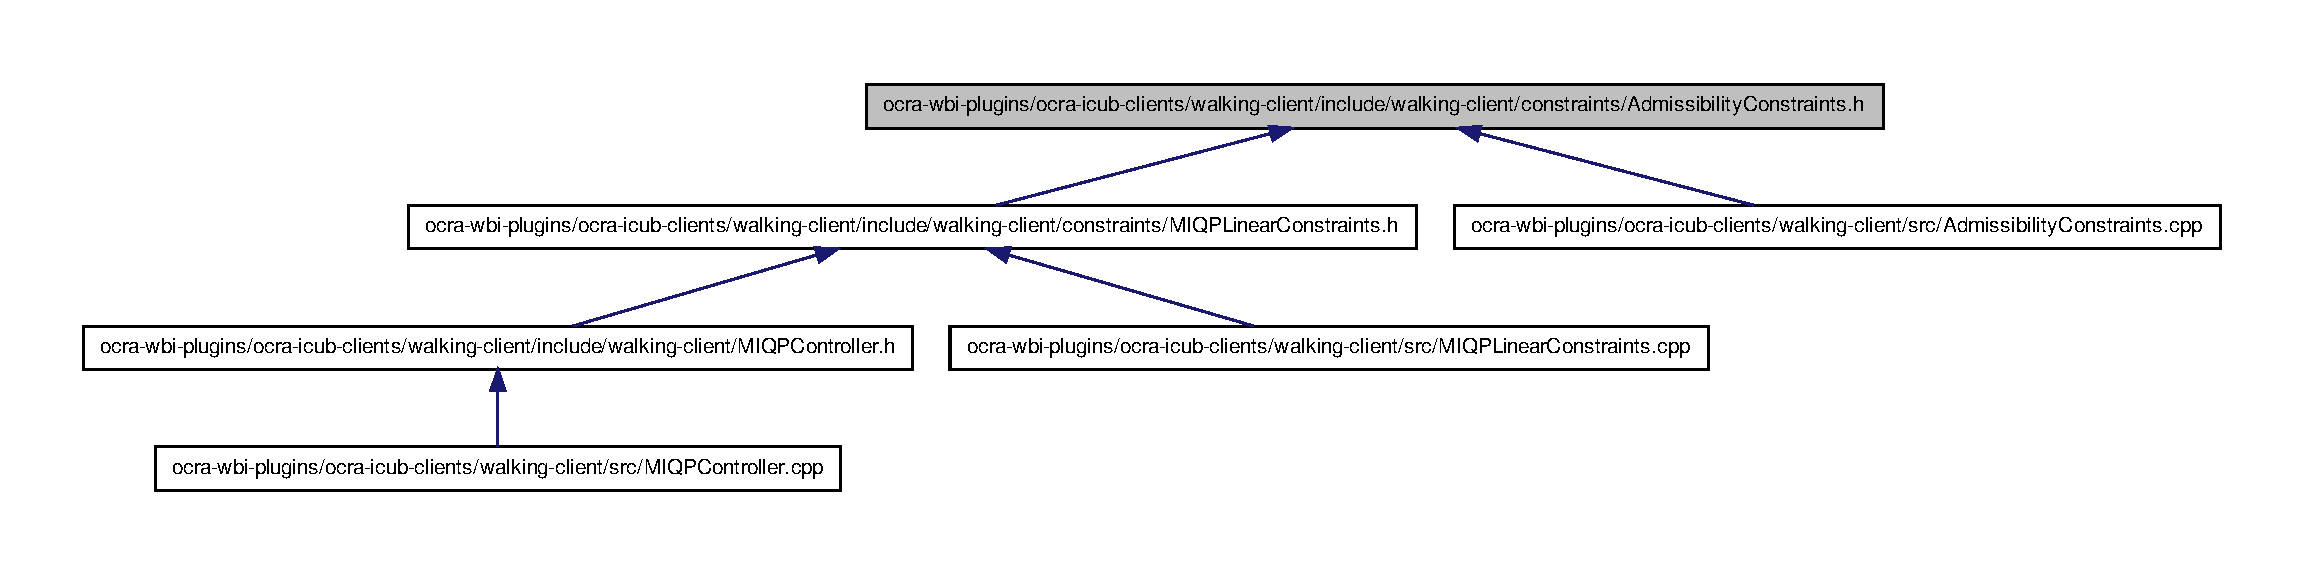
\includegraphics[width=350pt]{AdmissibilityConstraints_8h__dep__incl}
\end{center}
\end{figure}
\subsection*{\-Classes}
\begin{DoxyCompactItemize}
\item 
class \hyperlink{classAdmissibilityConstraints}{\-Admissibility\-Constraints}
\end{DoxyCompactItemize}

\hypertarget{Bounding_8h}{\section{ocra-\/wbi-\/plugins/ocra-\/icub-\/clients/walking-\/client/include/walking-\/client/constraints/\-Bounding.h \-File \-Reference}
\label{Bounding_8h}\index{ocra-\/wbi-\/plugins/ocra-\/icub-\/clients/walking-\/client/include/walking-\/client/constraints/\-Bounding.\-h@{ocra-\/wbi-\/plugins/ocra-\/icub-\/clients/walking-\/client/include/walking-\/client/constraints/\-Bounding.\-h}}
}
{\ttfamily \#include \char`\"{}walking-\/client/constraints/\-Constraint.\-h\char`\"{}}\*
\-Include dependency graph for \-Bounding.\-h\-:\nopagebreak
\begin{figure}[H]
\begin{center}
\leavevmode
\includegraphics[width=350pt]{Bounding_8h__incl}
\end{center}
\end{figure}
\-This graph shows which files directly or indirectly include this file\-:
\nopagebreak
\begin{figure}[H]
\begin{center}
\leavevmode
\includegraphics[width=350pt]{Bounding_8h__dep__incl}
\end{center}
\end{figure}
\subsection*{\-Classes}
\begin{DoxyCompactItemize}
\item 
class \hyperlink{classBounding}{\-Bounding}
\end{DoxyCompactItemize}

\hypertarget{Constancy_8h}{\section{ocra-\/wbi-\/plugins/ocra-\/icub-\/clients/walking-\/client/include/walking-\/client/constraints/\-Constancy.h \-File \-Reference}
\label{Constancy_8h}\index{ocra-\/wbi-\/plugins/ocra-\/icub-\/clients/walking-\/client/include/walking-\/client/constraints/\-Constancy.\-h@{ocra-\/wbi-\/plugins/ocra-\/icub-\/clients/walking-\/client/include/walking-\/client/constraints/\-Constancy.\-h}}
}
{\ttfamily \#include \char`\"{}walking-\/client/constraints/\-Constraint.\-h\char`\"{}}\*
\-Include dependency graph for \-Constancy.\-h\-:\nopagebreak
\begin{figure}[H]
\begin{center}
\leavevmode
\includegraphics[width=350pt]{Constancy_8h__incl}
\end{center}
\end{figure}
\-This graph shows which files directly or indirectly include this file\-:\nopagebreak
\begin{figure}[H]
\begin{center}
\leavevmode
\includegraphics[width=350pt]{Constancy_8h__dep__incl}
\end{center}
\end{figure}
\subsection*{\-Classes}
\begin{DoxyCompactItemize}
\item 
class \hyperlink{classConstancy}{\-Constancy}
\end{DoxyCompactItemize}

\hypertarget{Constraint_8h}{}\section{Constraint.\+h File Reference}
\label{Constraint_8h}\index{Constraint.\+h@{Constraint.\+h}}


Declaration file of the Constraint class.  


{\ttfamily \#include \char`\"{}ocra/optim/\+Variable.\+h\char`\"{}}\\*
{\ttfamily \#include \char`\"{}ocra/optim/\+Function.\+h\char`\"{}}\\*
{\ttfamily \#include \char`\"{}ocra/optim/\+Function\+Interface\+Mapping.\+h\char`\"{}}\\*
{\ttfamily \#include $<$ocra/util/\+Macros.\+h$>$}\\*
{\ttfamily \#include $<$boost/static\+\_\+assert.\+hpp$>$}\\*
{\ttfamily \#include $<$boost/type\+\_\+traits/is\+\_\+base\+\_\+of.\+hpp$>$}\\*
{\ttfamily \#include \char`\"{}ocra/optim/\+Linear\+Function.\+h\char`\"{}}\\*
{\ttfamily \#include \char`\"{}ocra/optim/\+Bound\+Function.\+h\char`\"{}}\\*
{\ttfamily \#include \char`\"{}ocra/optim/\+Identity\+Function.\+h\char`\"{}}\\*
{\ttfamily \#include \char`\"{}ocra/optim/\+Diagonal\+Linear\+Function.\+h\char`\"{}}\\*
Include dependency graph for Constraint.\+h\+:
\nopagebreak
\begin{figure}[H]
\begin{center}
\leavevmode
\includegraphics[width=350pt]{d8/df0/Constraint_8h__incl}
\end{center}
\end{figure}
This graph shows which files directly or indirectly include this file\+:
\nopagebreak
\begin{figure}[H]
\begin{center}
\leavevmode
\includegraphics[width=350pt]{df/d6c/Constraint_8h__dep__incl}
\end{center}
\end{figure}
\subsection*{Classes}
\begin{DoxyCompactItemize}
\item 
class \hyperlink{classocra_1_1Constraint}{ocra\+::\+Constraint$<$ T $>$}
\begin{DoxyCompactList}\small\item\em Constraint class. \end{DoxyCompactList}\item 
class \hyperlink{classocra_1_1Constraint_3_01Function_01_4}{ocra\+::\+Constraint$<$ Function $>$}
\end{DoxyCompactItemize}
\subsection*{Namespaces}
\begin{DoxyCompactItemize}
\item 
 \hyperlink{namespaceocra}{ocra}
\begin{DoxyCompactList}\small\item\em Optimization-\/based Robot \hyperlink{classocra_1_1Controller}{Controller} namespace. a library of classes to write and solve optimization problems dedicated to the control of multi-\/body systems. \end{DoxyCompactList}\end{DoxyCompactItemize}
\subsection*{Typedefs}
\begin{DoxyCompactItemize}
\item 
typedef Constraint$<$ Function $>$ \hyperlink{namespaceocra_af10341108ce661566aad00908668e2b1}{ocra\+::\+Generic\+Constraint}
\item 
typedef Constraint$<$ Linear\+Function $>$ \hyperlink{namespaceocra_ae8b87cf4099be3efc3b410019ad2046e}{ocra\+::\+Linear\+Constraint}
\item 
typedef Constraint$<$ Bound\+Function $>$ \hyperlink{namespaceocra_a6e55fff77635080219964abc301abf18}{ocra\+::\+Bound\+Constraint}
\item 
typedef Constraint$<$ Identity\+Function $>$ \hyperlink{namespaceocra_a5fc023ff4ef8f4b0cdf410e088090731}{ocra\+::\+Identity\+Constraint}
\item 
typedef Constraint$<$ Diagonal\+Linear\+Function $>$ \hyperlink{namespaceocra_ab310e2c53f5e52ec3aba0a832f7dc79e}{ocra\+::\+Diagonal\+Linear\+Constraint}
\end{DoxyCompactItemize}
\subsection*{Enumerations}
\begin{DoxyCompactItemize}
\item 
enum \hyperlink{namespaceocra_aedff92662043a7f15dc263363db7939b}{ocra\+::e\+Constraint\+Type} \{ \\*
\hyperlink{namespaceocra_aedff92662043a7f15dc263363db7939ba267dfa231e99fa27e51c96f7f254edeb}{ocra\+::\+C\+S\+T\+R\+\_\+\+E\+Q\+U\+A\+L\+\_\+\+Z\+E\+RO} =0, 
\hyperlink{namespaceocra_aedff92662043a7f15dc263363db7939ba3c53e336c7001d9e91cbab87fed6c617}{ocra\+::\+C\+S\+T\+R\+\_\+\+E\+Q\+U\+A\+L\+\_\+B}, 
\hyperlink{namespaceocra_aedff92662043a7f15dc263363db7939baaaef445573e3c2d9fef8c9cf8c2beedc}{ocra\+::\+C\+S\+T\+R\+\_\+\+L\+O\+W\+E\+R\+\_\+\+Z\+E\+RO}, 
\hyperlink{namespaceocra_aedff92662043a7f15dc263363db7939ba243df44f270fea35b7fc08565adf5e64}{ocra\+::\+C\+S\+T\+R\+\_\+\+L\+O\+W\+E\+R\+\_\+U}, 
\\*
\hyperlink{namespaceocra_aedff92662043a7f15dc263363db7939ba72ba216f8bf5c8482b450645f3c3985e}{ocra\+::\+C\+S\+T\+R\+\_\+\+G\+R\+E\+A\+T\+E\+R\+\_\+\+Z\+E\+RO}, 
\hyperlink{namespaceocra_aedff92662043a7f15dc263363db7939ba9e056f131217f1d13cde9b6a1b41f5de}{ocra\+::\+C\+S\+T\+R\+\_\+\+G\+R\+E\+A\+T\+E\+R\+\_\+L}, 
\hyperlink{namespaceocra_aedff92662043a7f15dc263363db7939bacde9128c1d54f28ad292f5e61a30d8d1}{ocra\+::\+C\+S\+T\+R\+\_\+\+L\+O\+W\+E\+R\+\_\+\+A\+N\+D\+\_\+\+G\+R\+E\+A\+T\+ER}
 \}
\end{DoxyCompactItemize}


\subsection{Detailed Description}
Declaration file of the Constraint class. 

Copyright (C) 2009 C\+E\+A/\+D\+R\+T/\+L\+I\+S\+T/\+D\+T\+S\+I/\+S\+R\+CI Copyright (C) 2010 C\+E\+A/\+D\+R\+T/\+L\+I\+S\+T/\+D\+I\+A\+S\+I/\+L\+SI

\begin{DoxyAuthor}{Author}
Escande Adrien 
\end{DoxyAuthor}
\begin{DoxyDate}{Date}
09/04/24
\end{DoxyDate}
File history\+:
\begin{DoxyItemize}
\item 10/06/10 Escande Adrien\+: mapping of Function Interface is deferred to function\+Interface\+Mapping, adding lower and upper bounds to inequality constraints. 
\end{DoxyItemize}
\hypertarget{ContactConfigEnforcement_8h}{\section{ocra-\/wbi-\/plugins/ocra-\/icub-\/clients/walking-\/client/include/walking-\/client/constraints/\-Contact\-Config\-Enforcement.h \-File \-Reference}
\label{ContactConfigEnforcement_8h}\index{ocra-\/wbi-\/plugins/ocra-\/icub-\/clients/walking-\/client/include/walking-\/client/constraints/\-Contact\-Config\-Enforcement.\-h@{ocra-\/wbi-\/plugins/ocra-\/icub-\/clients/walking-\/client/include/walking-\/client/constraints/\-Contact\-Config\-Enforcement.\-h}}
}
{\ttfamily \#include \char`\"{}walking-\/client/constraints/constraint.\-h\char`\"{}}\*
\-Include dependency graph for \-Contact\-Config\-Enforcement.\-h\-:
\nopagebreak
\begin{figure}[H]
\begin{center}
\leavevmode
\includegraphics[width=350pt]{ContactConfigEnforcement_8h__incl}
\end{center}
\end{figure}
\-This graph shows which files directly or indirectly include this file\-:
\nopagebreak
\begin{figure}[H]
\begin{center}
\leavevmode
\includegraphics[width=350pt]{ContactConfigEnforcement_8h__dep__incl}
\end{center}
\end{figure}
\subsection*{\-Classes}
\begin{DoxyCompactItemize}
\item 
class \hyperlink{classContactConfigEnforcement}{\-Contact\-Config\-Enforcement}
\end{DoxyCompactItemize}

\hypertarget{ContactConfigHistory_8h}{\section{ocra-\/wbi-\/plugins/ocra-\/icub-\/clients/walking-\/client/include/walking-\/client/constraints/\-Contact\-Config\-History.h \-File \-Reference}
\label{ContactConfigHistory_8h}\index{ocra-\/wbi-\/plugins/ocra-\/icub-\/clients/walking-\/client/include/walking-\/client/constraints/\-Contact\-Config\-History.\-h@{ocra-\/wbi-\/plugins/ocra-\/icub-\/clients/walking-\/client/include/walking-\/client/constraints/\-Contact\-Config\-History.\-h}}
}
{\ttfamily \#include \char`\"{}walking-\/client/constraints/constraint.\-h\char`\"{}}\*
\-Include dependency graph for \-Contact\-Config\-History.\-h\-:\nopagebreak
\begin{figure}[H]
\begin{center}
\leavevmode
\includegraphics[width=350pt]{ContactConfigHistory_8h__incl}
\end{center}
\end{figure}
\-This graph shows which files directly or indirectly include this file\-:\nopagebreak
\begin{figure}[H]
\begin{center}
\leavevmode
\includegraphics[width=350pt]{ContactConfigHistory_8h__dep__incl}
\end{center}
\end{figure}
\subsection*{\-Classes}
\begin{DoxyCompactItemize}
\item 
class \hyperlink{classContactConfigHistory}{\-Contact\-Config\-History}
\end{DoxyCompactItemize}

\hypertarget{MIQPLinearConstraints_8h}{\section{ocra-\/wbi-\/plugins/ocra-\/icub-\/clients/walking-\/client/include/walking-\/client/constraints/\-M\-I\-Q\-P\-Linear\-Constraints.h \-File \-Reference}
\label{MIQPLinearConstraints_8h}\index{ocra-\/wbi-\/plugins/ocra-\/icub-\/clients/walking-\/client/include/walking-\/client/constraints/\-M\-I\-Q\-P\-Linear\-Constraints.\-h@{ocra-\/wbi-\/plugins/ocra-\/icub-\/clients/walking-\/client/include/walking-\/client/constraints/\-M\-I\-Q\-P\-Linear\-Constraints.\-h}}
}
{\ttfamily \#include \char`\"{}walking-\/client/constraints/\-Shape\-Constraints.\-h\char`\"{}}\*
{\ttfamily \#include \char`\"{}walking-\/client/constraints/\-Admissibility\-Constraints.\-h\char`\"{}}\*
{\ttfamily \#include \char`\"{}walking-\/client/\-Step\-Controller.\-h\char`\"{}}\*
{\ttfamily \#include \char`\"{}walking-\/client/\-Base\-Of\-Support.\-h\char`\"{}}\*
\-Include dependency graph for \-M\-I\-Q\-P\-Linear\-Constraints.\-h\-:\nopagebreak
\begin{figure}[H]
\begin{center}
\leavevmode
\includegraphics[width=350pt]{MIQPLinearConstraints_8h__incl}
\end{center}
\end{figure}
\-This graph shows which files directly or indirectly include this file\-:\nopagebreak
\begin{figure}[H]
\begin{center}
\leavevmode
\includegraphics[width=350pt]{MIQPLinearConstraints_8h__dep__incl}
\end{center}
\end{figure}
\subsection*{\-Classes}
\begin{DoxyCompactItemize}
\item 
class \hyperlink{classMIQPLinearConstraints}{\-M\-I\-Q\-P\-Linear\-Constraints}
\end{DoxyCompactItemize}

\hypertarget{Sequentiality_8h}{\section{ocra-\/wbi-\/plugins/ocra-\/icub-\/clients/walking-\/client/include/walking-\/client/constraints/\-Sequentiality.h \-File \-Reference}
\label{Sequentiality_8h}\index{ocra-\/wbi-\/plugins/ocra-\/icub-\/clients/walking-\/client/include/walking-\/client/constraints/\-Sequentiality.\-h@{ocra-\/wbi-\/plugins/ocra-\/icub-\/clients/walking-\/client/include/walking-\/client/constraints/\-Sequentiality.\-h}}
}
{\ttfamily \#include \char`\"{}walking-\/client/constraints/\-Constraint.\-h\char`\"{}}\*
\-Include dependency graph for \-Sequentiality.\-h\-:
\nopagebreak
\begin{figure}[H]
\begin{center}
\leavevmode
\includegraphics[width=350pt]{Sequentiality_8h__incl}
\end{center}
\end{figure}
\-This graph shows which files directly or indirectly include this file\-:
\nopagebreak
\begin{figure}[H]
\begin{center}
\leavevmode
\includegraphics[width=350pt]{Sequentiality_8h__dep__incl}
\end{center}
\end{figure}
\subsection*{\-Classes}
\begin{DoxyCompactItemize}
\item 
class \hyperlink{classSequentiality}{\-Sequentiality}
\end{DoxyCompactItemize}

\hypertarget{ShapeConstraints_8h}{\section{ocra-\/wbi-\/plugins/ocra-\/icub-\/clients/walking-\/client/include/walking-\/client/constraints/\-Shape\-Constraints.h \-File \-Reference}
\label{ShapeConstraints_8h}\index{ocra-\/wbi-\/plugins/ocra-\/icub-\/clients/walking-\/client/include/walking-\/client/constraints/\-Shape\-Constraints.\-h@{ocra-\/wbi-\/plugins/ocra-\/icub-\/clients/walking-\/client/include/walking-\/client/constraints/\-Shape\-Constraints.\-h}}
}
{\ttfamily \#include \char`\"{}walking-\/client/constraints/\-Constraint.\-h\char`\"{}}\*
{\ttfamily \#include \char`\"{}walking-\/client/constraints/\-Bounding.\-h\char`\"{}}\*
{\ttfamily \#include \char`\"{}walking-\/client/constraints/constancy.\-h\char`\"{}}\*
{\ttfamily \#include \char`\"{}walking-\/client/constraints/sequentiality.\-h\char`\"{}}\*
\-Include dependency graph for \-Shape\-Constraints.\-h\-:\nopagebreak
\begin{figure}[H]
\begin{center}
\leavevmode
\includegraphics[width=350pt]{ShapeConstraints_8h__incl}
\end{center}
\end{figure}
\-This graph shows which files directly or indirectly include this file\-:
\nopagebreak
\begin{figure}[H]
\begin{center}
\leavevmode
\includegraphics[width=350pt]{ShapeConstraints_8h__dep__incl}
\end{center}
\end{figure}
\subsection*{\-Classes}
\begin{DoxyCompactItemize}
\item 
class \hyperlink{classShapeConstraints}{\-Shape\-Constraints}
\end{DoxyCompactItemize}

\hypertarget{SingleSupport_8h}{\section{ocra-\/wbi-\/plugins/ocra-\/icub-\/clients/walking-\/client/include/walking-\/client/constraints/\-Single\-Support.h \-File \-Reference}
\label{SingleSupport_8h}\index{ocra-\/wbi-\/plugins/ocra-\/icub-\/clients/walking-\/client/include/walking-\/client/constraints/\-Single\-Support.\-h@{ocra-\/wbi-\/plugins/ocra-\/icub-\/clients/walking-\/client/include/walking-\/client/constraints/\-Single\-Support.\-h}}
}
{\ttfamily \#include \char`\"{}walking-\/client/constraints/constraint.\-h\char`\"{}}\*
\-Include dependency graph for \-Single\-Support.\-h\-:\nopagebreak
\begin{figure}[H]
\begin{center}
\leavevmode
\includegraphics[width=350pt]{SingleSupport_8h__incl}
\end{center}
\end{figure}
\-This graph shows which files directly or indirectly include this file\-:
\nopagebreak
\begin{figure}[H]
\begin{center}
\leavevmode
\includegraphics[width=350pt]{SingleSupport_8h__dep__incl}
\end{center}
\end{figure}
\subsection*{\-Classes}
\begin{DoxyCompactItemize}
\item 
class \hyperlink{classSingleSupport}{\-Single\-Support}
\end{DoxyCompactItemize}

\hypertarget{SSDSAlternation_8h}{\section{ocra-\/wbi-\/plugins/ocra-\/icub-\/clients/walking-\/client/include/walking-\/client/constraints/\-S\-S\-D\-S\-Alternation.h \-File \-Reference}
\label{SSDSAlternation_8h}\index{ocra-\/wbi-\/plugins/ocra-\/icub-\/clients/walking-\/client/include/walking-\/client/constraints/\-S\-S\-D\-S\-Alternation.\-h@{ocra-\/wbi-\/plugins/ocra-\/icub-\/clients/walking-\/client/include/walking-\/client/constraints/\-S\-S\-D\-S\-Alternation.\-h}}
}
{\ttfamily \#include \char`\"{}walking-\/client/constraints/\-Constraint.\-h\char`\"{}}\*
\-Include dependency graph for \-S\-S\-D\-S\-Alternation.\-h\-:
\nopagebreak
\begin{figure}[H]
\begin{center}
\leavevmode
\includegraphics[width=350pt]{SSDSAlternation_8h__incl}
\end{center}
\end{figure}
\-This graph shows which files directly or indirectly include this file\-:\nopagebreak
\begin{figure}[H]
\begin{center}
\leavevmode
\includegraphics[width=350pt]{SSDSAlternation_8h__dep__incl}
\end{center}
\end{figure}
\subsection*{\-Classes}
\begin{DoxyCompactItemize}
\item 
class \hyperlink{classSSDSAlternation}{\-S\-S\-D\-S\-Alternation}
\end{DoxyCompactItemize}

\hypertarget{constraintsStructs_8h}{\section{ocra-\/wbi-\/plugins/ocra-\/icub-\/clients/walking-\/client/include/walking-\/client/constraints\-Structs.h \-File \-Reference}
\label{constraintsStructs_8h}\index{ocra-\/wbi-\/plugins/ocra-\/icub-\/clients/walking-\/client/include/walking-\/client/constraints\-Structs.\-h@{ocra-\/wbi-\/plugins/ocra-\/icub-\/clients/walking-\/client/include/walking-\/client/constraints\-Structs.\-h}}
}
{\ttfamily \#include $<$\-Eigen/\-Core$>$}\*
\-Include dependency graph for constraints\-Structs.\-h\-:\nopagebreak
\begin{figure}[H]
\begin{center}
\leavevmode
\includegraphics[width=350pt]{constraintsStructs_8h__incl}
\end{center}
\end{figure}
\subsection*{\-Classes}
\begin{DoxyCompactItemize}
\item 
struct \hyperlink{structShapeConstraintsStruct}{\-Shape\-Constraints\-Struct}
\item 
struct \hyperlink{structShapeConstraintsStruct_1_1boundingStruct}{\-Shape\-Constraints\-Struct\-::bounding\-Struct}
\item 
struct \hyperlink{structShapeConstraintsStruct_1_1constancyStruct}{\-Shape\-Constraints\-Struct\-::constancy\-Struct}
\item 
struct \hyperlink{structShapeConstraintsStruct_1_1sequentialityStruct}{\-Shape\-Constraints\-Struct\-::sequentiality\-Struct}
\item 
struct \hyperlink{structAdmissibilityConstraintsStruct}{\-Admissibility\-Constraints\-Struct}
\item 
struct \hyperlink{structAdmissibilityConstraintsStruct_1_1SSandDSAlternation}{\-Admissibility\-Constraints\-Struct\-::\-S\-Sand\-D\-S\-Alternation}
\item 
struct \hyperlink{structAdmissibilityConstraintsStruct_1_1SingleSupport}{\-Admissibility\-Constraints\-Struct\-::\-Single\-Support}
\item 
struct \hyperlink{structAdmissibilityConstraintsStruct_1_1ContactConfigurationHistory}{\-Admissibility\-Constraints\-Struct\-::\-Contact\-Configuration\-History}
\item 
struct \hyperlink{structAdmissibilityConstraintsStruct_1_1ContactConfigurationEnforcement}{\-Admissibility\-Constraints\-Struct\-::\-Contact\-Configuration\-Enforcement}
\end{DoxyCompactItemize}
\subsection*{\-Enumerations}
\begin{DoxyCompactItemize}
\item 
enum \hyperlink{constraintsStructs_8h_aa9522c516e629788f7eac510abe3dadd}{\-C\-O\-N\-S\-T\-R\-A\-I\-N\-T\-S\-\_\-\-T\-Y\-P\-E} \{ \hyperlink{constraintsStructs_8h_aa9522c516e629788f7eac510abe3dadda143086ff46ca8e1c216820c2aa29f1dc}{\-S\-H\-A\-P\-E\-\_\-\-C\-O\-N\-S\-T\-R\-A\-I\-N\-T\-S} =  0, 
\hyperlink{constraintsStructs_8h_aa9522c516e629788f7eac510abe3dadda976183e2a10817758df0c380039efef8}{\-A\-D\-M\-I\-S\-S\-I\-B\-I\-L\-I\-T\-Y\-\_\-\-C\-O\-N\-S\-T\-R\-A\-I\-N\-T\-S}, 
\hyperlink{constraintsStructs_8h_aa9522c516e629788f7eac510abe3dadda07f6e01814e8a347915e2b02228963f2}{\-W\-A\-L\-K\-I\-N\-G\-\_\-\-C\-O\-N\-S\-T\-R\-A\-I\-N\-T\-S}
 \}
\end{DoxyCompactItemize}


\subsection{\-Enumeration \-Type \-Documentation}
\hypertarget{constraintsStructs_8h_aa9522c516e629788f7eac510abe3dadd}{\index{constraints\-Structs.\-h@{constraints\-Structs.\-h}!\-C\-O\-N\-S\-T\-R\-A\-I\-N\-T\-S\-\_\-\-T\-Y\-P\-E@{\-C\-O\-N\-S\-T\-R\-A\-I\-N\-T\-S\-\_\-\-T\-Y\-P\-E}}
\index{\-C\-O\-N\-S\-T\-R\-A\-I\-N\-T\-S\-\_\-\-T\-Y\-P\-E@{\-C\-O\-N\-S\-T\-R\-A\-I\-N\-T\-S\-\_\-\-T\-Y\-P\-E}!constraintsStructs.h@{constraints\-Structs.\-h}}
\subsubsection[{\-C\-O\-N\-S\-T\-R\-A\-I\-N\-T\-S\-\_\-\-T\-Y\-P\-E}]{\setlength{\rightskip}{0pt plus 5cm}enum {\bf \-C\-O\-N\-S\-T\-R\-A\-I\-N\-T\-S\-\_\-\-T\-Y\-P\-E}}}\label{constraintsStructs_8h_aa9522c516e629788f7eac510abe3dadd}
\begin{Desc}
\item[\-Enumerator\-: ]\par
\begin{description}
\index{\-S\-H\-A\-P\-E\-\_\-\-C\-O\-N\-S\-T\-R\-A\-I\-N\-T\-S@{\-S\-H\-A\-P\-E\-\_\-\-C\-O\-N\-S\-T\-R\-A\-I\-N\-T\-S}!constraints\-Structs.\-h@{constraints\-Structs.\-h}}\index{constraints\-Structs.\-h@{constraints\-Structs.\-h}!\-S\-H\-A\-P\-E\-\_\-\-C\-O\-N\-S\-T\-R\-A\-I\-N\-T\-S@{\-S\-H\-A\-P\-E\-\_\-\-C\-O\-N\-S\-T\-R\-A\-I\-N\-T\-S}}\item[{\em 
\hypertarget{constraintsStructs_8h_aa9522c516e629788f7eac510abe3dadda143086ff46ca8e1c216820c2aa29f1dc}{\-S\-H\-A\-P\-E\-\_\-\-C\-O\-N\-S\-T\-R\-A\-I\-N\-T\-S}\label{constraintsStructs_8h_aa9522c516e629788f7eac510abe3dadda143086ff46ca8e1c216820c2aa29f1dc}
}]\index{\-A\-D\-M\-I\-S\-S\-I\-B\-I\-L\-I\-T\-Y\-\_\-\-C\-O\-N\-S\-T\-R\-A\-I\-N\-T\-S@{\-A\-D\-M\-I\-S\-S\-I\-B\-I\-L\-I\-T\-Y\-\_\-\-C\-O\-N\-S\-T\-R\-A\-I\-N\-T\-S}!constraints\-Structs.\-h@{constraints\-Structs.\-h}}\index{constraints\-Structs.\-h@{constraints\-Structs.\-h}!\-A\-D\-M\-I\-S\-S\-I\-B\-I\-L\-I\-T\-Y\-\_\-\-C\-O\-N\-S\-T\-R\-A\-I\-N\-T\-S@{\-A\-D\-M\-I\-S\-S\-I\-B\-I\-L\-I\-T\-Y\-\_\-\-C\-O\-N\-S\-T\-R\-A\-I\-N\-T\-S}}\item[{\em 
\hypertarget{constraintsStructs_8h_aa9522c516e629788f7eac510abe3dadda976183e2a10817758df0c380039efef8}{\-A\-D\-M\-I\-S\-S\-I\-B\-I\-L\-I\-T\-Y\-\_\-\-C\-O\-N\-S\-T\-R\-A\-I\-N\-T\-S}\label{constraintsStructs_8h_aa9522c516e629788f7eac510abe3dadda976183e2a10817758df0c380039efef8}
}]\index{\-W\-A\-L\-K\-I\-N\-G\-\_\-\-C\-O\-N\-S\-T\-R\-A\-I\-N\-T\-S@{\-W\-A\-L\-K\-I\-N\-G\-\_\-\-C\-O\-N\-S\-T\-R\-A\-I\-N\-T\-S}!constraints\-Structs.\-h@{constraints\-Structs.\-h}}\index{constraints\-Structs.\-h@{constraints\-Structs.\-h}!\-W\-A\-L\-K\-I\-N\-G\-\_\-\-C\-O\-N\-S\-T\-R\-A\-I\-N\-T\-S@{\-W\-A\-L\-K\-I\-N\-G\-\_\-\-C\-O\-N\-S\-T\-R\-A\-I\-N\-T\-S}}\item[{\em 
\hypertarget{constraintsStructs_8h_aa9522c516e629788f7eac510abe3dadda07f6e01814e8a347915e2b02228963f2}{\-W\-A\-L\-K\-I\-N\-G\-\_\-\-C\-O\-N\-S\-T\-R\-A\-I\-N\-T\-S}\label{constraintsStructs_8h_aa9522c516e629788f7eac510abe3dadda07f6e01814e8a347915e2b02228963f2}
}]\end{description}
\end{Desc}


\hypertarget{MIQPController_8h}{\section{ocra-\/wbi-\/plugins/ocra-\/icub-\/clients/walking-\/client/include/walking-\/client/\-M\-I\-Q\-P\-Controller.h \-File \-Reference}
\label{MIQPController_8h}\index{ocra-\/wbi-\/plugins/ocra-\/icub-\/clients/walking-\/client/include/walking-\/client/\-M\-I\-Q\-P\-Controller.\-h@{ocra-\/wbi-\/plugins/ocra-\/icub-\/clients/walking-\/client/include/walking-\/client/\-M\-I\-Q\-P\-Controller.\-h}}
}


\-A thread for launching trajectory generators.  


{\ttfamily \#include \char`\"{}gurobi\-\_\-c++.\-h\char`\"{}}\*
{\ttfamily \#include $<$walking-\/client/utils.\-h$>$}\*
{\ttfamily \#include $<$ocra-\/icub/\-Ocra\-Wbi\-Model.\-h$>$}\*
{\ttfamily \#include $<$yarp/os/\-Rate\-Thread.\-h$>$}\*
{\ttfamily \#include $<$\-Eigen/\-Dense$>$}\*
{\ttfamily \#include $<$\-Eigen/\-Lgsm$>$}\*
{\ttfamily \#include \char`\"{}unsupported/\-Eigen/\-Matrix\-Functions\char`\"{}}\*
{\ttfamily \#include $<$walking-\/client/constraints/\-M\-I\-Q\-P\-Linear\-Constraints.\-h$>$}\*
{\ttfamily \#include $<$walking-\/client/\-M\-I\-Q\-P\-State.\-h$>$}\*
{\ttfamily \#include \char`\"{}\-Gurobi.\-h\char`\"{}}\*
\-Include dependency graph for \-M\-I\-Q\-P\-Controller.\-h\-:
\nopagebreak
\begin{figure}[H]
\begin{center}
\leavevmode
\includegraphics[width=350pt]{MIQPController_8h__incl}
\end{center}
\end{figure}
\-This graph shows which files directly or indirectly include this file\-:\nopagebreak
\begin{figure}[H]
\begin{center}
\leavevmode
\includegraphics[width=350pt]{MIQPController_8h__dep__incl}
\end{center}
\end{figure}
\subsection*{\-Classes}
\begin{DoxyCompactItemize}
\item 
class \hyperlink{classMIQPController}{\-M\-I\-Q\-P\-Controller}
\end{DoxyCompactItemize}
\subsection*{\-Defines}
\begin{DoxyCompactItemize}
\item 
\#define \hyperlink{MIQPController_8h_aa2f26540ce870ca91503bb6746a52e69}{\-I\-N\-P\-U\-T\-\_\-\-V\-E\-C\-T\-O\-R\-\_\-\-S\-I\-Z\-E}~12
\item 
\#define \hyperlink{MIQPController_8h_ab0e06eaa253307db2bac3c9b0a9e6b10}{\-S\-T\-A\-T\-E\-\_\-\-V\-E\-C\-T\-O\-R\-\_\-\-S\-I\-Z\-E}~16
\end{DoxyCompactItemize}


\subsection{\-Detailed \-Description}
\-A thread for launching trajectory generators. \begin{DoxyAuthor}{\-Author}
\mbox{[}\-Jorhabib \-Eljaik\mbox{]}(\href{https://github.com/jeljaik}{\tt https\-://github.\-com/jeljaik}) 
\end{DoxyAuthor}
\begin{DoxyDate}{\-Date}
\-Feb 2017 
\end{DoxyDate}
\begin{DoxyCopyright}{\-Copyright}
\-G\-N\-U \-General \-Public \-License. 
\end{DoxyCopyright}


\subsection{\-Define \-Documentation}
\hypertarget{MIQPController_8h_aa2f26540ce870ca91503bb6746a52e69}{\index{\-M\-I\-Q\-P\-Controller.\-h@{\-M\-I\-Q\-P\-Controller.\-h}!\-I\-N\-P\-U\-T\-\_\-\-V\-E\-C\-T\-O\-R\-\_\-\-S\-I\-Z\-E@{\-I\-N\-P\-U\-T\-\_\-\-V\-E\-C\-T\-O\-R\-\_\-\-S\-I\-Z\-E}}
\index{\-I\-N\-P\-U\-T\-\_\-\-V\-E\-C\-T\-O\-R\-\_\-\-S\-I\-Z\-E@{\-I\-N\-P\-U\-T\-\_\-\-V\-E\-C\-T\-O\-R\-\_\-\-S\-I\-Z\-E}!MIQPController.h@{\-M\-I\-Q\-P\-Controller.\-h}}
\subsubsection[{\-I\-N\-P\-U\-T\-\_\-\-V\-E\-C\-T\-O\-R\-\_\-\-S\-I\-Z\-E}]{\setlength{\rightskip}{0pt plus 5cm}\#define {\bf \-I\-N\-P\-U\-T\-\_\-\-V\-E\-C\-T\-O\-R\-\_\-\-S\-I\-Z\-E}~12}}\label{MIQPController_8h_aa2f26540ce870ca91503bb6746a52e69}
\hypertarget{MIQPController_8h_ab0e06eaa253307db2bac3c9b0a9e6b10}{\index{\-M\-I\-Q\-P\-Controller.\-h@{\-M\-I\-Q\-P\-Controller.\-h}!\-S\-T\-A\-T\-E\-\_\-\-V\-E\-C\-T\-O\-R\-\_\-\-S\-I\-Z\-E@{\-S\-T\-A\-T\-E\-\_\-\-V\-E\-C\-T\-O\-R\-\_\-\-S\-I\-Z\-E}}
\index{\-S\-T\-A\-T\-E\-\_\-\-V\-E\-C\-T\-O\-R\-\_\-\-S\-I\-Z\-E@{\-S\-T\-A\-T\-E\-\_\-\-V\-E\-C\-T\-O\-R\-\_\-\-S\-I\-Z\-E}!MIQPController.h@{\-M\-I\-Q\-P\-Controller.\-h}}
\subsubsection[{\-S\-T\-A\-T\-E\-\_\-\-V\-E\-C\-T\-O\-R\-\_\-\-S\-I\-Z\-E}]{\setlength{\rightskip}{0pt plus 5cm}\#define {\bf \-S\-T\-A\-T\-E\-\_\-\-V\-E\-C\-T\-O\-R\-\_\-\-S\-I\-Z\-E}~16}}\label{MIQPController_8h_ab0e06eaa253307db2bac3c9b0a9e6b10}

\hypertarget{MIQPState_8h}{\section{ocra-\/wbi-\/plugins/ocra-\/icub-\/clients/walking-\/client/include/walking-\/client/\-M\-I\-Q\-P\-State.h \-File \-Reference}
\label{MIQPState_8h}\index{ocra-\/wbi-\/plugins/ocra-\/icub-\/clients/walking-\/client/include/walking-\/client/\-M\-I\-Q\-P\-State.\-h@{ocra-\/wbi-\/plugins/ocra-\/icub-\/clients/walking-\/client/include/walking-\/client/\-M\-I\-Q\-P\-State.\-h}}
}
{\ttfamily \#include $<$\-Eigen/\-Dense$>$}\*
{\ttfamily \#include $<$ocra-\/icub/\-Ocra\-Wbi\-Model.\-h$>$}\*
{\ttfamily \#include $<$ocra/util/\-Errors\-Helper.\-h$>$}\*
{\ttfamily \#include \char`\"{}walking-\/client/utils.\-h\char`\"{}}\*
{\ttfamily \#include $<$ocra-\/icub/\-Utilities.\-h$>$}\*
\-Include dependency graph for \-M\-I\-Q\-P\-State.\-h\-:
\nopagebreak
\begin{figure}[H]
\begin{center}
\leavevmode
\includegraphics[width=350pt]{MIQPState_8h__incl}
\end{center}
\end{figure}
\-This graph shows which files directly or indirectly include this file\-:
\nopagebreak
\begin{figure}[H]
\begin{center}
\leavevmode
\includegraphics[width=350pt]{MIQPState_8h__dep__incl}
\end{center}
\end{figure}
\subsection*{\-Classes}
\begin{DoxyCompactItemize}
\item 
class \hyperlink{classMIQPState}{\-M\-I\-Q\-P\-State}
\begin{DoxyCompactList}\small\item\em \-Takes care of updating the state defined for the \-M\-I\-Q\-P problem. \end{DoxyCompactList}\end{DoxyCompactItemize}

\hypertarget{StepController_8h}{\section{ocra-\/wbi-\/plugins/ocra-\/icub-\/clients/walking-\/client/include/walking-\/client/\-Step\-Controller.h \-File \-Reference}
\label{StepController_8h}\index{ocra-\/wbi-\/plugins/ocra-\/icub-\/clients/walking-\/client/include/walking-\/client/\-Step\-Controller.\-h@{ocra-\/wbi-\/plugins/ocra-\/icub-\/clients/walking-\/client/include/walking-\/client/\-Step\-Controller.\-h}}
}
{\ttfamily \#include $<$ocra-\/recipes/\-Trajectory\-Thread.\-h$>$}\*
{\ttfamily \#include \char`\"{}walking-\/client/utils.\-h\char`\"{}}\*
\-Include dependency graph for \-Step\-Controller.\-h\-:\nopagebreak
\begin{figure}[H]
\begin{center}
\leavevmode
\includegraphics[width=350pt]{StepController_8h__incl}
\end{center}
\end{figure}
\-This graph shows which files directly or indirectly include this file\-:
\nopagebreak
\begin{figure}[H]
\begin{center}
\leavevmode
\includegraphics[width=350pt]{StepController_8h__dep__incl}
\end{center}
\end{figure}
\subsection*{\-Classes}
\begin{DoxyCompactItemize}
\item 
class \hyperlink{classStepController}{\-Step\-Controller}
\end{DoxyCompactItemize}

\hypertarget{utils_8h}{\section{ocra-\/wbi-\/plugins/ocra-\/icub-\/clients/walking-\/client/include/walking-\/client/utils.h \-File \-Reference}
\label{utils_8h}\index{ocra-\/wbi-\/plugins/ocra-\/icub-\/clients/walking-\/client/include/walking-\/client/utils.\-h@{ocra-\/wbi-\/plugins/ocra-\/icub-\/clients/walking-\/client/include/walking-\/client/utils.\-h}}
}
\-This graph shows which files directly or indirectly include this file\-:
\nopagebreak
\begin{figure}[H]
\begin{center}
\leavevmode
\includegraphics[width=350pt]{utils_8h__dep__incl}
\end{center}
\end{figure}
\subsection*{\-Classes}
\begin{DoxyCompactItemize}
\item 
struct \hyperlink{structsingleStepTestParams}{single\-Step\-Test\-Params}
\item 
struct \hyperlink{structMIQPParameters}{\-M\-I\-Q\-P\-Parameters}
\end{DoxyCompactItemize}
\subsection*{\-Defines}
\begin{DoxyCompactItemize}
\item 
\#define \hyperlink{utils_8h_ab0e06eaa253307db2bac3c9b0a9e6b10}{\-S\-T\-A\-T\-E\-\_\-\-V\-E\-C\-T\-O\-R\-\_\-\-S\-I\-Z\-E}~16
\item 
\#define \hyperlink{utils_8h_aa2f26540ce870ca91503bb6746a52e69}{\-I\-N\-P\-U\-T\-\_\-\-V\-E\-C\-T\-O\-R\-\_\-\-S\-I\-Z\-E}~12
\end{DoxyCompactItemize}
\subsection*{\-Enumerations}
\begin{DoxyCompactItemize}
\item 
enum \hyperlink{utils_8h_a4b6a8e135f90bd56e5a57a60efb42529}{\-F\-O\-O\-T} \{ \hyperlink{utils_8h_a4b6a8e135f90bd56e5a57a60efb42529a7760daad9db1ede8c57b06189deca9f3}{\-L\-E\-F\-T\-\_\-\-F\-O\-O\-T}, 
\hyperlink{utils_8h_a4b6a8e135f90bd56e5a57a60efb42529ace119c66af60ac0781b137aa87d7be62}{\-R\-I\-G\-H\-T\-\_\-\-F\-O\-O\-T}, 
\hyperlink{ZmpController_8h_a4b6a8e135f90bd56e5a57a60efb42529a7760daad9db1ede8c57b06189deca9f3}{\-L\-E\-F\-T\-\_\-\-F\-O\-O\-T}, 
\hyperlink{ZmpController_8h_a4b6a8e135f90bd56e5a57a60efb42529ace119c66af60ac0781b137aa87d7be62}{\-R\-I\-G\-H\-T\-\_\-\-F\-O\-O\-T}
 \}
\item 
enum \hyperlink{utils_8h_afc01479a47f5a87462a54b6a9e11fffa}{\-Zmp\-Test\-Type} \{ \hyperlink{utils_8h_afc01479a47f5a87462a54b6a9e11fffaa648ff770c850b8352c3306c1659e8157}{\-Z\-M\-P\-\_\-\-C\-O\-N\-S\-T\-A\-N\-T\-\_\-\-R\-E\-F\-E\-R\-E\-N\-C\-E} = 0, 
\hyperlink{utils_8h_afc01479a47f5a87462a54b6a9e11fffaa97cb99b5fec95c1f2945d3b33455b139}{\-Z\-M\-P\-\_\-\-V\-A\-R\-Y\-I\-N\-G\-\_\-\-R\-E\-F\-E\-R\-E\-N\-C\-E}, 
\hyperlink{utils_8h_afc01479a47f5a87462a54b6a9e11fffaad20e2ca429f4e3ba50e1de174c92af60}{\-C\-O\-M\-\_\-\-L\-I\-N\-\_\-\-V\-E\-L\-\_\-\-C\-O\-N\-S\-T\-A\-N\-T\-\_\-\-R\-E\-F\-E\-R\-E\-N\-C\-E}, 
\hyperlink{utils_8h_afc01479a47f5a87462a54b6a9e11fffaa4cf77e5736bd9a94342342d774b2e264}{\-S\-I\-N\-G\-L\-E\-\_\-\-S\-T\-E\-P}
 \}
\end{DoxyCompactItemize}


\subsection{\-Define \-Documentation}
\hypertarget{utils_8h_aa2f26540ce870ca91503bb6746a52e69}{\index{utils.\-h@{utils.\-h}!\-I\-N\-P\-U\-T\-\_\-\-V\-E\-C\-T\-O\-R\-\_\-\-S\-I\-Z\-E@{\-I\-N\-P\-U\-T\-\_\-\-V\-E\-C\-T\-O\-R\-\_\-\-S\-I\-Z\-E}}
\index{\-I\-N\-P\-U\-T\-\_\-\-V\-E\-C\-T\-O\-R\-\_\-\-S\-I\-Z\-E@{\-I\-N\-P\-U\-T\-\_\-\-V\-E\-C\-T\-O\-R\-\_\-\-S\-I\-Z\-E}!utils.h@{utils.\-h}}
\subsubsection[{\-I\-N\-P\-U\-T\-\_\-\-V\-E\-C\-T\-O\-R\-\_\-\-S\-I\-Z\-E}]{\setlength{\rightskip}{0pt plus 5cm}\#define {\bf \-I\-N\-P\-U\-T\-\_\-\-V\-E\-C\-T\-O\-R\-\_\-\-S\-I\-Z\-E}~12}}\label{utils_8h_aa2f26540ce870ca91503bb6746a52e69}
\hypertarget{utils_8h_ab0e06eaa253307db2bac3c9b0a9e6b10}{\index{utils.\-h@{utils.\-h}!\-S\-T\-A\-T\-E\-\_\-\-V\-E\-C\-T\-O\-R\-\_\-\-S\-I\-Z\-E@{\-S\-T\-A\-T\-E\-\_\-\-V\-E\-C\-T\-O\-R\-\_\-\-S\-I\-Z\-E}}
\index{\-S\-T\-A\-T\-E\-\_\-\-V\-E\-C\-T\-O\-R\-\_\-\-S\-I\-Z\-E@{\-S\-T\-A\-T\-E\-\_\-\-V\-E\-C\-T\-O\-R\-\_\-\-S\-I\-Z\-E}!utils.h@{utils.\-h}}
\subsubsection[{\-S\-T\-A\-T\-E\-\_\-\-V\-E\-C\-T\-O\-R\-\_\-\-S\-I\-Z\-E}]{\setlength{\rightskip}{0pt plus 5cm}\#define {\bf \-S\-T\-A\-T\-E\-\_\-\-V\-E\-C\-T\-O\-R\-\_\-\-S\-I\-Z\-E}~16}}\label{utils_8h_ab0e06eaa253307db2bac3c9b0a9e6b10}


\subsection{\-Enumeration \-Type \-Documentation}
\hypertarget{utils_8h_a4b6a8e135f90bd56e5a57a60efb42529}{\index{utils.\-h@{utils.\-h}!\-F\-O\-O\-T@{\-F\-O\-O\-T}}
\index{\-F\-O\-O\-T@{\-F\-O\-O\-T}!utils.h@{utils.\-h}}
\subsubsection[{\-F\-O\-O\-T}]{\setlength{\rightskip}{0pt plus 5cm}enum {\bf \-F\-O\-O\-T}}}\label{utils_8h_a4b6a8e135f90bd56e5a57a60efb42529}
\begin{Desc}
\item[\-Enumerator\-: ]\par
\begin{description}
\index{\-L\-E\-F\-T\-\_\-\-F\-O\-O\-T@{\-L\-E\-F\-T\-\_\-\-F\-O\-O\-T}!utils.\-h@{utils.\-h}}\index{utils.\-h@{utils.\-h}!\-L\-E\-F\-T\-\_\-\-F\-O\-O\-T@{\-L\-E\-F\-T\-\_\-\-F\-O\-O\-T}}\item[{\em 
\hypertarget{utils_8h_a4b6a8e135f90bd56e5a57a60efb42529a7760daad9db1ede8c57b06189deca9f3}{\-L\-E\-F\-T\-\_\-\-F\-O\-O\-T}\label{utils_8h_a4b6a8e135f90bd56e5a57a60efb42529a7760daad9db1ede8c57b06189deca9f3}
}]\index{\-R\-I\-G\-H\-T\-\_\-\-F\-O\-O\-T@{\-R\-I\-G\-H\-T\-\_\-\-F\-O\-O\-T}!utils.\-h@{utils.\-h}}\index{utils.\-h@{utils.\-h}!\-R\-I\-G\-H\-T\-\_\-\-F\-O\-O\-T@{\-R\-I\-G\-H\-T\-\_\-\-F\-O\-O\-T}}\item[{\em 
\hypertarget{utils_8h_a4b6a8e135f90bd56e5a57a60efb42529ace119c66af60ac0781b137aa87d7be62}{\-R\-I\-G\-H\-T\-\_\-\-F\-O\-O\-T}\label{utils_8h_a4b6a8e135f90bd56e5a57a60efb42529ace119c66af60ac0781b137aa87d7be62}
}]\index{\-L\-E\-F\-T\-\_\-\-F\-O\-O\-T@{\-L\-E\-F\-T\-\_\-\-F\-O\-O\-T}!utils.\-h@{utils.\-h}}\index{utils.\-h@{utils.\-h}!\-L\-E\-F\-T\-\_\-\-F\-O\-O\-T@{\-L\-E\-F\-T\-\_\-\-F\-O\-O\-T}}\item[{\em 
\hypertarget{utils_8h_a4b6a8e135f90bd56e5a57a60efb42529a7760daad9db1ede8c57b06189deca9f3}{\-L\-E\-F\-T\-\_\-\-F\-O\-O\-T}\label{utils_8h_a4b6a8e135f90bd56e5a57a60efb42529a7760daad9db1ede8c57b06189deca9f3}
}]\index{\-R\-I\-G\-H\-T\-\_\-\-F\-O\-O\-T@{\-R\-I\-G\-H\-T\-\_\-\-F\-O\-O\-T}!utils.\-h@{utils.\-h}}\index{utils.\-h@{utils.\-h}!\-R\-I\-G\-H\-T\-\_\-\-F\-O\-O\-T@{\-R\-I\-G\-H\-T\-\_\-\-F\-O\-O\-T}}\item[{\em 
\hypertarget{utils_8h_a4b6a8e135f90bd56e5a57a60efb42529ace119c66af60ac0781b137aa87d7be62}{\-R\-I\-G\-H\-T\-\_\-\-F\-O\-O\-T}\label{utils_8h_a4b6a8e135f90bd56e5a57a60efb42529ace119c66af60ac0781b137aa87d7be62}
}]\end{description}
\end{Desc}

\hypertarget{utils_8h_afc01479a47f5a87462a54b6a9e11fffa}{\index{utils.\-h@{utils.\-h}!\-Zmp\-Test\-Type@{\-Zmp\-Test\-Type}}
\index{\-Zmp\-Test\-Type@{\-Zmp\-Test\-Type}!utils.h@{utils.\-h}}
\subsubsection[{\-Zmp\-Test\-Type}]{\setlength{\rightskip}{0pt plus 5cm}enum {\bf \-Zmp\-Test\-Type}}}\label{utils_8h_afc01479a47f5a87462a54b6a9e11fffa}
\-Performs tests helpful to tune the gains used by the zmp and zmp preview controllers as well as the \-C\-O\-M task. \-See configure() for additional information. \begin{Desc}
\item[\-Enumerator\-: ]\par
\begin{description}
\index{\-Z\-M\-P\-\_\-\-C\-O\-N\-S\-T\-A\-N\-T\-\_\-\-R\-E\-F\-E\-R\-E\-N\-C\-E@{\-Z\-M\-P\-\_\-\-C\-O\-N\-S\-T\-A\-N\-T\-\_\-\-R\-E\-F\-E\-R\-E\-N\-C\-E}!utils.\-h@{utils.\-h}}\index{utils.\-h@{utils.\-h}!\-Z\-M\-P\-\_\-\-C\-O\-N\-S\-T\-A\-N\-T\-\_\-\-R\-E\-F\-E\-R\-E\-N\-C\-E@{\-Z\-M\-P\-\_\-\-C\-O\-N\-S\-T\-A\-N\-T\-\_\-\-R\-E\-F\-E\-R\-E\-N\-C\-E}}\item[{\em 
\hypertarget{utils_8h_afc01479a47f5a87462a54b6a9e11fffaa648ff770c850b8352c3306c1659e8157}{\-Z\-M\-P\-\_\-\-C\-O\-N\-S\-T\-A\-N\-T\-\_\-\-R\-E\-F\-E\-R\-E\-N\-C\-E}\label{utils_8h_afc01479a47f5a87462a54b6a9e11fffaa648ff770c850b8352c3306c1659e8157}
}]\index{\-Z\-M\-P\-\_\-\-V\-A\-R\-Y\-I\-N\-G\-\_\-\-R\-E\-F\-E\-R\-E\-N\-C\-E@{\-Z\-M\-P\-\_\-\-V\-A\-R\-Y\-I\-N\-G\-\_\-\-R\-E\-F\-E\-R\-E\-N\-C\-E}!utils.\-h@{utils.\-h}}\index{utils.\-h@{utils.\-h}!\-Z\-M\-P\-\_\-\-V\-A\-R\-Y\-I\-N\-G\-\_\-\-R\-E\-F\-E\-R\-E\-N\-C\-E@{\-Z\-M\-P\-\_\-\-V\-A\-R\-Y\-I\-N\-G\-\_\-\-R\-E\-F\-E\-R\-E\-N\-C\-E}}\item[{\em 
\hypertarget{utils_8h_afc01479a47f5a87462a54b6a9e11fffaa97cb99b5fec95c1f2945d3b33455b139}{\-Z\-M\-P\-\_\-\-V\-A\-R\-Y\-I\-N\-G\-\_\-\-R\-E\-F\-E\-R\-E\-N\-C\-E}\label{utils_8h_afc01479a47f5a87462a54b6a9e11fffaa97cb99b5fec95c1f2945d3b33455b139}
}]\index{\-C\-O\-M\-\_\-\-L\-I\-N\-\_\-\-V\-E\-L\-\_\-\-C\-O\-N\-S\-T\-A\-N\-T\-\_\-\-R\-E\-F\-E\-R\-E\-N\-C\-E@{\-C\-O\-M\-\_\-\-L\-I\-N\-\_\-\-V\-E\-L\-\_\-\-C\-O\-N\-S\-T\-A\-N\-T\-\_\-\-R\-E\-F\-E\-R\-E\-N\-C\-E}!utils.\-h@{utils.\-h}}\index{utils.\-h@{utils.\-h}!\-C\-O\-M\-\_\-\-L\-I\-N\-\_\-\-V\-E\-L\-\_\-\-C\-O\-N\-S\-T\-A\-N\-T\-\_\-\-R\-E\-F\-E\-R\-E\-N\-C\-E@{\-C\-O\-M\-\_\-\-L\-I\-N\-\_\-\-V\-E\-L\-\_\-\-C\-O\-N\-S\-T\-A\-N\-T\-\_\-\-R\-E\-F\-E\-R\-E\-N\-C\-E}}\item[{\em 
\hypertarget{utils_8h_afc01479a47f5a87462a54b6a9e11fffaad20e2ca429f4e3ba50e1de174c92af60}{\-C\-O\-M\-\_\-\-L\-I\-N\-\_\-\-V\-E\-L\-\_\-\-C\-O\-N\-S\-T\-A\-N\-T\-\_\-\-R\-E\-F\-E\-R\-E\-N\-C\-E}\label{utils_8h_afc01479a47f5a87462a54b6a9e11fffaad20e2ca429f4e3ba50e1de174c92af60}
}]\index{\-S\-I\-N\-G\-L\-E\-\_\-\-S\-T\-E\-P@{\-S\-I\-N\-G\-L\-E\-\_\-\-S\-T\-E\-P}!utils.\-h@{utils.\-h}}\index{utils.\-h@{utils.\-h}!\-S\-I\-N\-G\-L\-E\-\_\-\-S\-T\-E\-P@{\-S\-I\-N\-G\-L\-E\-\_\-\-S\-T\-E\-P}}\item[{\em 
\hypertarget{utils_8h_afc01479a47f5a87462a54b6a9e11fffaa4cf77e5736bd9a94342342d774b2e264}{\-S\-I\-N\-G\-L\-E\-\_\-\-S\-T\-E\-P}\label{utils_8h_afc01479a47f5a87462a54b6a9e11fffaa4cf77e5736bd9a94342342d774b2e264}
}]\end{description}
\end{Desc}


\hypertarget{WalkingClient_8h}{\section{ocra-\/wbi-\/plugins/ocra-\/icub-\/clients/walking-\/client/include/walking-\/client/\-Walking\-Client.h \-File \-Reference}
\label{WalkingClient_8h}\index{ocra-\/wbi-\/plugins/ocra-\/icub-\/clients/walking-\/client/include/walking-\/client/\-Walking\-Client.\-h@{ocra-\/wbi-\/plugins/ocra-\/icub-\/clients/walking-\/client/include/walking-\/client/\-Walking\-Client.\-h}}
}
{\ttfamily \#include $<$ocra-\/icub/\-Icub\-Client.\-h$>$}\*
{\ttfamily \#include $<$ocra-\/recipes/\-Trajectory\-Thread.\-h$>$}\*
{\ttfamily \#include $<$ocra-\/recipes/\-Controller\-Client.\-h$>$}\*
{\ttfamily \#include $<$ocra/util/\-Eigen\-Utilities.\-h$>$}\*
{\ttfamily \#include \char`\"{}walking-\/client/\-Zmp\-Preview\-Controller.\-h\char`\"{}}\*
{\ttfamily \#include \char`\"{}walking-\/client/\-Zmp\-Controller.\-h\char`\"{}}\*
{\ttfamily \#include $<$ocra/util/\-File\-Operations.\-h$>$}\*
{\ttfamily \#include $<$yarp/os/\-Time.\-h$>$}\*
\-Include dependency graph for \-Walking\-Client.\-h\-:
\nopagebreak
\begin{figure}[H]
\begin{center}
\leavevmode
\includegraphics[width=350pt]{WalkingClient_8h__incl}
\end{center}
\end{figure}
\-This graph shows which files directly or indirectly include this file\-:
\nopagebreak
\begin{figure}[H]
\begin{center}
\leavevmode
\includegraphics[width=350pt]{WalkingClient_8h__dep__incl}
\end{center}
\end{figure}
\subsection*{\-Classes}
\begin{DoxyCompactItemize}
\item 
class \hyperlink{classWalkingClient}{\-Walking\-Client}
\end{DoxyCompactItemize}
\subsection*{\-Enumerations}
\begin{DoxyCompactItemize}
\item 
enum \hyperlink{WalkingClient_8h_afc01479a47f5a87462a54b6a9e11fffa}{\-Zmp\-Test\-Type} \{ \hyperlink{WalkingClient_8h_afc01479a47f5a87462a54b6a9e11fffaa648ff770c850b8352c3306c1659e8157}{\-Z\-M\-P\-\_\-\-C\-O\-N\-S\-T\-A\-N\-T\-\_\-\-R\-E\-F\-E\-R\-E\-N\-C\-E} = 0, 
\hyperlink{WalkingClient_8h_afc01479a47f5a87462a54b6a9e11fffaa97cb99b5fec95c1f2945d3b33455b139}{\-Z\-M\-P\-\_\-\-V\-A\-R\-Y\-I\-N\-G\-\_\-\-R\-E\-F\-E\-R\-E\-N\-C\-E}, 
\hyperlink{WalkingClient_8h_afc01479a47f5a87462a54b6a9e11fffaad20e2ca429f4e3ba50e1de174c92af60}{\-C\-O\-M\-\_\-\-L\-I\-N\-\_\-\-V\-E\-L\-\_\-\-C\-O\-N\-S\-T\-A\-N\-T\-\_\-\-R\-E\-F\-E\-R\-E\-N\-C\-E}
 \}
\end{DoxyCompactItemize}


\subsection{\-Enumeration \-Type \-Documentation}
\hypertarget{WalkingClient_8h_afc01479a47f5a87462a54b6a9e11fffa}{\index{\-Walking\-Client.\-h@{\-Walking\-Client.\-h}!\-Zmp\-Test\-Type@{\-Zmp\-Test\-Type}}
\index{\-Zmp\-Test\-Type@{\-Zmp\-Test\-Type}!WalkingClient.h@{\-Walking\-Client.\-h}}
\subsubsection[{\-Zmp\-Test\-Type}]{\setlength{\rightskip}{0pt plus 5cm}enum {\bf \-Zmp\-Test\-Type}}}\label{WalkingClient_8h_afc01479a47f5a87462a54b6a9e11fffa}
\-Performs tests helpful to tune the gains used by the zmp and zmp preview controllers as well as the \-C\-O\-M task. \-See configure() for additional information. \begin{Desc}
\item[\-Enumerator\-: ]\par
\begin{description}
\index{\-Z\-M\-P\-\_\-\-C\-O\-N\-S\-T\-A\-N\-T\-\_\-\-R\-E\-F\-E\-R\-E\-N\-C\-E@{\-Z\-M\-P\-\_\-\-C\-O\-N\-S\-T\-A\-N\-T\-\_\-\-R\-E\-F\-E\-R\-E\-N\-C\-E}!\-Walking\-Client.\-h@{\-Walking\-Client.\-h}}\index{\-Walking\-Client.\-h@{\-Walking\-Client.\-h}!\-Z\-M\-P\-\_\-\-C\-O\-N\-S\-T\-A\-N\-T\-\_\-\-R\-E\-F\-E\-R\-E\-N\-C\-E@{\-Z\-M\-P\-\_\-\-C\-O\-N\-S\-T\-A\-N\-T\-\_\-\-R\-E\-F\-E\-R\-E\-N\-C\-E}}\item[{\em 
\hypertarget{WalkingClient_8h_afc01479a47f5a87462a54b6a9e11fffaa648ff770c850b8352c3306c1659e8157}{\-Z\-M\-P\-\_\-\-C\-O\-N\-S\-T\-A\-N\-T\-\_\-\-R\-E\-F\-E\-R\-E\-N\-C\-E}\label{WalkingClient_8h_afc01479a47f5a87462a54b6a9e11fffaa648ff770c850b8352c3306c1659e8157}
}]\index{\-Z\-M\-P\-\_\-\-V\-A\-R\-Y\-I\-N\-G\-\_\-\-R\-E\-F\-E\-R\-E\-N\-C\-E@{\-Z\-M\-P\-\_\-\-V\-A\-R\-Y\-I\-N\-G\-\_\-\-R\-E\-F\-E\-R\-E\-N\-C\-E}!\-Walking\-Client.\-h@{\-Walking\-Client.\-h}}\index{\-Walking\-Client.\-h@{\-Walking\-Client.\-h}!\-Z\-M\-P\-\_\-\-V\-A\-R\-Y\-I\-N\-G\-\_\-\-R\-E\-F\-E\-R\-E\-N\-C\-E@{\-Z\-M\-P\-\_\-\-V\-A\-R\-Y\-I\-N\-G\-\_\-\-R\-E\-F\-E\-R\-E\-N\-C\-E}}\item[{\em 
\hypertarget{WalkingClient_8h_afc01479a47f5a87462a54b6a9e11fffaa97cb99b5fec95c1f2945d3b33455b139}{\-Z\-M\-P\-\_\-\-V\-A\-R\-Y\-I\-N\-G\-\_\-\-R\-E\-F\-E\-R\-E\-N\-C\-E}\label{WalkingClient_8h_afc01479a47f5a87462a54b6a9e11fffaa97cb99b5fec95c1f2945d3b33455b139}
}]\index{\-C\-O\-M\-\_\-\-L\-I\-N\-\_\-\-V\-E\-L\-\_\-\-C\-O\-N\-S\-T\-A\-N\-T\-\_\-\-R\-E\-F\-E\-R\-E\-N\-C\-E@{\-C\-O\-M\-\_\-\-L\-I\-N\-\_\-\-V\-E\-L\-\_\-\-C\-O\-N\-S\-T\-A\-N\-T\-\_\-\-R\-E\-F\-E\-R\-E\-N\-C\-E}!\-Walking\-Client.\-h@{\-Walking\-Client.\-h}}\index{\-Walking\-Client.\-h@{\-Walking\-Client.\-h}!\-C\-O\-M\-\_\-\-L\-I\-N\-\_\-\-V\-E\-L\-\_\-\-C\-O\-N\-S\-T\-A\-N\-T\-\_\-\-R\-E\-F\-E\-R\-E\-N\-C\-E@{\-C\-O\-M\-\_\-\-L\-I\-N\-\_\-\-V\-E\-L\-\_\-\-C\-O\-N\-S\-T\-A\-N\-T\-\_\-\-R\-E\-F\-E\-R\-E\-N\-C\-E}}\item[{\em 
\hypertarget{WalkingClient_8h_afc01479a47f5a87462a54b6a9e11fffaad20e2ca429f4e3ba50e1de174c92af60}{\-C\-O\-M\-\_\-\-L\-I\-N\-\_\-\-V\-E\-L\-\_\-\-C\-O\-N\-S\-T\-A\-N\-T\-\_\-\-R\-E\-F\-E\-R\-E\-N\-C\-E}\label{WalkingClient_8h_afc01479a47f5a87462a54b6a9e11fffaad20e2ca429f4e3ba50e1de174c92af60}
}]\end{description}
\end{Desc}


\hypertarget{ZmpController_8h}{\section{ocra-\/wbi-\/plugins/ocra-\/icub-\/clients/walking-\/client/include/walking-\/client/\-Zmp\-Controller.h \-File \-Reference}
\label{ZmpController_8h}\index{ocra-\/wbi-\/plugins/ocra-\/icub-\/clients/walking-\/client/include/walking-\/client/\-Zmp\-Controller.\-h@{ocra-\/wbi-\/plugins/ocra-\/icub-\/clients/walking-\/client/include/walking-\/client/\-Zmp\-Controller.\-h}}
}
{\ttfamily \#include $<$ocra-\/icub/\-Utilities.\-h$>$}\*
{\ttfamily \#include $<$ocra/util/\-Errors\-Helper.\-h$>$}\*
{\ttfamily \#include $<$ocra/util/\-Eigen\-Utilities.\-h$>$}\*
{\ttfamily \#include $<$ocra/control/\-Task\-State.\-h$>$}\*
{\ttfamily \#include $<$ocra-\/recipes/\-Task\-Connection.\-h$>$}\*
{\ttfamily \#include $<$\-Eigen/\-Dense$>$}\*
{\ttfamily \#include $<$vector$>$}\*
\-Include dependency graph for \-Zmp\-Controller.\-h\-:\nopagebreak
\begin{figure}[H]
\begin{center}
\leavevmode
\includegraphics[width=350pt]{ZmpController_8h__incl}
\end{center}
\end{figure}
\-This graph shows which files directly or indirectly include this file\-:\nopagebreak
\begin{figure}[H]
\begin{center}
\leavevmode
\includegraphics[width=350pt]{ZmpController_8h__dep__incl}
\end{center}
\end{figure}
\subsection*{\-Classes}
\begin{DoxyCompactItemize}
\item 
struct \hyperlink{structZmpControllerParams}{\-Zmp\-Controller\-Params}
\item 
class \hyperlink{classZmpController}{\-Zmp\-Controller}
\begin{DoxyCompactList}\small\item\em \-Implementes a \-Z\-M\-P controller as a force set point regulator. \end{DoxyCompactList}\end{DoxyCompactItemize}
\subsection*{\-Enumerations}
\begin{DoxyCompactItemize}
\item 
enum \hyperlink{ZmpController_8h_a4b6a8e135f90bd56e5a57a60efb42529}{\-F\-O\-O\-T} \{ \hyperlink{ZmpController_8h_a4b6a8e135f90bd56e5a57a60efb42529a7760daad9db1ede8c57b06189deca9f3}{\-L\-E\-F\-T\-\_\-\-F\-O\-O\-T}, 
\hyperlink{ZmpController_8h_a4b6a8e135f90bd56e5a57a60efb42529ace119c66af60ac0781b137aa87d7be62}{\-R\-I\-G\-H\-T\-\_\-\-F\-O\-O\-T}
 \}
\end{DoxyCompactItemize}


\subsection{\-Enumeration \-Type \-Documentation}
\hypertarget{ZmpController_8h_a4b6a8e135f90bd56e5a57a60efb42529}{\index{\-Zmp\-Controller.\-h@{\-Zmp\-Controller.\-h}!\-F\-O\-O\-T@{\-F\-O\-O\-T}}
\index{\-F\-O\-O\-T@{\-F\-O\-O\-T}!ZmpController.h@{\-Zmp\-Controller.\-h}}
\subsubsection[{\-F\-O\-O\-T}]{\setlength{\rightskip}{0pt plus 5cm}enum {\bf \-F\-O\-O\-T}}}\label{ZmpController_8h_a4b6a8e135f90bd56e5a57a60efb42529}
\begin{Desc}
\item[\-Enumerator\-: ]\par
\begin{description}
\index{\-L\-E\-F\-T\-\_\-\-F\-O\-O\-T@{\-L\-E\-F\-T\-\_\-\-F\-O\-O\-T}!\-Zmp\-Controller.\-h@{\-Zmp\-Controller.\-h}}\index{\-Zmp\-Controller.\-h@{\-Zmp\-Controller.\-h}!\-L\-E\-F\-T\-\_\-\-F\-O\-O\-T@{\-L\-E\-F\-T\-\_\-\-F\-O\-O\-T}}\item[{\em 
\hypertarget{ZmpController_8h_a4b6a8e135f90bd56e5a57a60efb42529a7760daad9db1ede8c57b06189deca9f3}{\-L\-E\-F\-T\-\_\-\-F\-O\-O\-T}\label{ZmpController_8h_a4b6a8e135f90bd56e5a57a60efb42529a7760daad9db1ede8c57b06189deca9f3}
}]\index{\-R\-I\-G\-H\-T\-\_\-\-F\-O\-O\-T@{\-R\-I\-G\-H\-T\-\_\-\-F\-O\-O\-T}!\-Zmp\-Controller.\-h@{\-Zmp\-Controller.\-h}}\index{\-Zmp\-Controller.\-h@{\-Zmp\-Controller.\-h}!\-R\-I\-G\-H\-T\-\_\-\-F\-O\-O\-T@{\-R\-I\-G\-H\-T\-\_\-\-F\-O\-O\-T}}\item[{\em 
\hypertarget{ZmpController_8h_a4b6a8e135f90bd56e5a57a60efb42529ace119c66af60ac0781b137aa87d7be62}{\-R\-I\-G\-H\-T\-\_\-\-F\-O\-O\-T}\label{ZmpController_8h_a4b6a8e135f90bd56e5a57a60efb42529ace119c66af60ac0781b137aa87d7be62}
}]\end{description}
\end{Desc}


\hypertarget{ZmpPreviewController_8h}{\section{ocra-\/wbi-\/plugins/ocra-\/icub-\/clients/walking-\/client/include/walking-\/client/\-Zmp\-Preview\-Controller.h \-File \-Reference}
\label{ZmpPreviewController_8h}\index{ocra-\/wbi-\/plugins/ocra-\/icub-\/clients/walking-\/client/include/walking-\/client/\-Zmp\-Preview\-Controller.\-h@{ocra-\/wbi-\/plugins/ocra-\/icub-\/clients/walking-\/client/include/walking-\/client/\-Zmp\-Preview\-Controller.\-h}}
}
{\ttfamily \#include $<$ocra-\/icub/\-Utilities.\-h$>$}\*
{\ttfamily \#include $<$ocra/util/\-Errors\-Helper.\-h$>$}\*
{\ttfamily \#include $<$\-Eigen/\-Dense$>$}\*
{\ttfamily \#include $<$vector$>$}\*
\-Include dependency graph for \-Zmp\-Preview\-Controller.\-h\-:\nopagebreak
\begin{figure}[H]
\begin{center}
\leavevmode
\includegraphics[width=350pt]{ZmpPreviewController_8h__incl}
\end{center}
\end{figure}
\-This graph shows which files directly or indirectly include this file\-:\nopagebreak
\begin{figure}[H]
\begin{center}
\leavevmode
\includegraphics[width=350pt]{ZmpPreviewController_8h__dep__incl}
\end{center}
\end{figure}
\subsection*{\-Classes}
\begin{DoxyCompactItemize}
\item 
struct \hyperlink{structZmpPreviewParams}{\-Zmp\-Preview\-Params}
\item 
class \hyperlink{classZmpPreviewController}{\-Zmp\-Preview\-Controller}
\begin{DoxyCompactList}\small\item\em \-Implementes an extended \-Z\-M\-P preview controller as an unconstrained \-Q\-P problem. \end{DoxyCompactList}\end{DoxyCompactItemize}

\hypertarget{AdmissibilityConstraints_8cpp}{\section{ocra-\/wbi-\/plugins/ocra-\/icub-\/clients/walking-\/client/src/\-Admissibility\-Constraints.cpp \-File \-Reference}
\label{AdmissibilityConstraints_8cpp}\index{ocra-\/wbi-\/plugins/ocra-\/icub-\/clients/walking-\/client/src/\-Admissibility\-Constraints.\-cpp@{ocra-\/wbi-\/plugins/ocra-\/icub-\/clients/walking-\/client/src/\-Admissibility\-Constraints.\-cpp}}
}
{\ttfamily \#include \char`\"{}walking-\/client/constraints/\-Admissibility\-Constraints.\-h\char`\"{}}\*
\-Include dependency graph for \-Admissibility\-Constraints.\-cpp\-:\nopagebreak
\begin{figure}[H]
\begin{center}
\leavevmode
\includegraphics[width=350pt]{AdmissibilityConstraints_8cpp__incl}
\end{center}
\end{figure}

\hypertarget{BaseOfSupport_8cpp}{\section{ocra-\/wbi-\/plugins/ocra-\/icub-\/clients/walking-\/client/src/\-Base\-Of\-Support.cpp \-File \-Reference}
\label{BaseOfSupport_8cpp}\index{ocra-\/wbi-\/plugins/ocra-\/icub-\/clients/walking-\/client/src/\-Base\-Of\-Support.\-cpp@{ocra-\/wbi-\/plugins/ocra-\/icub-\/clients/walking-\/client/src/\-Base\-Of\-Support.\-cpp}}
}
{\ttfamily \#include \char`\"{}walking-\/client/\-Base\-Of\-Support.\-h\char`\"{}}\*
\-Include dependency graph for \-Base\-Of\-Support.\-cpp\-:
\nopagebreak
\begin{figure}[H]
\begin{center}
\leavevmode
\includegraphics[width=350pt]{BaseOfSupport_8cpp__incl}
\end{center}
\end{figure}

\hypertarget{Bounding_8cpp}{\section{ocra-\/wbi-\/plugins/ocra-\/icub-\/clients/walking-\/client/src/\-Bounding.cpp \-File \-Reference}
\label{Bounding_8cpp}\index{ocra-\/wbi-\/plugins/ocra-\/icub-\/clients/walking-\/client/src/\-Bounding.\-cpp@{ocra-\/wbi-\/plugins/ocra-\/icub-\/clients/walking-\/client/src/\-Bounding.\-cpp}}
}
{\ttfamily \#include \char`\"{}walking-\/client/constraints/\-Bounding.\-h\char`\"{}}\*
\-Include dependency graph for \-Bounding.\-cpp\-:\nopagebreak
\begin{figure}[H]
\begin{center}
\leavevmode
\includegraphics[width=350pt]{Bounding_8cpp__incl}
\end{center}
\end{figure}

\hypertarget{Constancy_8cpp}{\section{ocra-\/wbi-\/plugins/ocra-\/icub-\/clients/walking-\/client/src/\-Constancy.cpp \-File \-Reference}
\label{Constancy_8cpp}\index{ocra-\/wbi-\/plugins/ocra-\/icub-\/clients/walking-\/client/src/\-Constancy.\-cpp@{ocra-\/wbi-\/plugins/ocra-\/icub-\/clients/walking-\/client/src/\-Constancy.\-cpp}}
}
{\ttfamily \#include \char`\"{}walking-\/client/constraints/\-Constancy.\-h\char`\"{}}\*
\-Include dependency graph for \-Constancy.\-cpp\-:\nopagebreak
\begin{figure}[H]
\begin{center}
\leavevmode
\includegraphics[width=350pt]{Constancy_8cpp__incl}
\end{center}
\end{figure}

\hypertarget{ContactConfigEnforcement_8cpp}{\section{ocra-\/wbi-\/plugins/ocra-\/icub-\/clients/walking-\/client/src/\-Contact\-Config\-Enforcement.cpp \-File \-Reference}
\label{ContactConfigEnforcement_8cpp}\index{ocra-\/wbi-\/plugins/ocra-\/icub-\/clients/walking-\/client/src/\-Contact\-Config\-Enforcement.\-cpp@{ocra-\/wbi-\/plugins/ocra-\/icub-\/clients/walking-\/client/src/\-Contact\-Config\-Enforcement.\-cpp}}
}
{\ttfamily \#include \char`\"{}walking-\/client/constraints/\-Contact\-Config\-Enforcement.\-h\char`\"{}}\*
\-Include dependency graph for \-Contact\-Config\-Enforcement.\-cpp\-:\nopagebreak
\begin{figure}[H]
\begin{center}
\leavevmode
\includegraphics[width=350pt]{ContactConfigEnforcement_8cpp__incl}
\end{center}
\end{figure}

\hypertarget{ContactConfigHistory_8cpp}{\section{ocra-\/wbi-\/plugins/ocra-\/icub-\/clients/walking-\/client/src/\-Contact\-Config\-History.cpp \-File \-Reference}
\label{ContactConfigHistory_8cpp}\index{ocra-\/wbi-\/plugins/ocra-\/icub-\/clients/walking-\/client/src/\-Contact\-Config\-History.\-cpp@{ocra-\/wbi-\/plugins/ocra-\/icub-\/clients/walking-\/client/src/\-Contact\-Config\-History.\-cpp}}
}
{\ttfamily \#include \char`\"{}walking-\/client/constraints/\-Contact\-Config\-History.\-h\char`\"{}}\*
\-Include dependency graph for \-Contact\-Config\-History.\-cpp\-:
\nopagebreak
\begin{figure}[H]
\begin{center}
\leavevmode
\includegraphics[width=350pt]{ContactConfigHistory_8cpp__incl}
\end{center}
\end{figure}

\hypertarget{MIQPController_8cpp}{\section{ocra-\/wbi-\/plugins/ocra-\/icub-\/clients/walking-\/client/src/\-M\-I\-Q\-P\-Controller.cpp \-File \-Reference}
\label{MIQPController_8cpp}\index{ocra-\/wbi-\/plugins/ocra-\/icub-\/clients/walking-\/client/src/\-M\-I\-Q\-P\-Controller.\-cpp@{ocra-\/wbi-\/plugins/ocra-\/icub-\/clients/walking-\/client/src/\-M\-I\-Q\-P\-Controller.\-cpp}}
}
{\ttfamily \#include \char`\"{}walking-\/client/\-M\-I\-Q\-P\-Controller.\-h\char`\"{}}\*
\-Include dependency graph for \-M\-I\-Q\-P\-Controller.\-cpp\-:\nopagebreak
\begin{figure}[H]
\begin{center}
\leavevmode
\includegraphics[width=350pt]{MIQPController_8cpp__incl}
\end{center}
\end{figure}

\hypertarget{MIQPLinearConstraints_8cpp}{\section{ocra-\/wbi-\/plugins/ocra-\/icub-\/clients/walking-\/client/src/\-M\-I\-Q\-P\-Linear\-Constraints.cpp \-File \-Reference}
\label{MIQPLinearConstraints_8cpp}\index{ocra-\/wbi-\/plugins/ocra-\/icub-\/clients/walking-\/client/src/\-M\-I\-Q\-P\-Linear\-Constraints.\-cpp@{ocra-\/wbi-\/plugins/ocra-\/icub-\/clients/walking-\/client/src/\-M\-I\-Q\-P\-Linear\-Constraints.\-cpp}}
}
{\ttfamily \#include \char`\"{}walking-\/client/constraints/\-M\-I\-Q\-P\-Linear\-Constraints.\-h\char`\"{}}\*
\-Include dependency graph for \-M\-I\-Q\-P\-Linear\-Constraints.\-cpp\-:\nopagebreak
\begin{figure}[H]
\begin{center}
\leavevmode
\includegraphics[width=350pt]{MIQPLinearConstraints_8cpp__incl}
\end{center}
\end{figure}

\hypertarget{MIQPState_8cpp}{\section{ocra-\/wbi-\/plugins/ocra-\/icub-\/clients/walking-\/client/src/\-M\-I\-Q\-P\-State.cpp \-File \-Reference}
\label{MIQPState_8cpp}\index{ocra-\/wbi-\/plugins/ocra-\/icub-\/clients/walking-\/client/src/\-M\-I\-Q\-P\-State.\-cpp@{ocra-\/wbi-\/plugins/ocra-\/icub-\/clients/walking-\/client/src/\-M\-I\-Q\-P\-State.\-cpp}}
}
{\ttfamily \#include \char`\"{}walking-\/client/\-M\-I\-Q\-P\-State.\-h\char`\"{}}\*
\-Include dependency graph for \-M\-I\-Q\-P\-State.\-cpp\-:
\nopagebreak
\begin{figure}[H]
\begin{center}
\leavevmode
\includegraphics[width=350pt]{MIQPState_8cpp__incl}
\end{center}
\end{figure}
\subsection*{\-Functions}
\begin{DoxyCompactItemize}
\item 
std\-::ostream \& \hyperlink{MIQPState_8cpp_ad32751f8094f2fa0f7c1ebca5eabf9df}{operator$<$$<$} (std\-::ostream \&out, const \hyperlink{classMIQPState}{\-M\-I\-Q\-P\-State} \&state)
\end{DoxyCompactItemize}


\subsection{\-Function \-Documentation}
\hypertarget{MIQPState_8cpp_ad32751f8094f2fa0f7c1ebca5eabf9df}{\index{\-M\-I\-Q\-P\-State.\-cpp@{\-M\-I\-Q\-P\-State.\-cpp}!operator$<$$<$@{operator$<$$<$}}
\index{operator$<$$<$@{operator$<$$<$}!MIQPState.cpp@{\-M\-I\-Q\-P\-State.\-cpp}}
\subsubsection[{operator$<$$<$}]{\setlength{\rightskip}{0pt plus 5cm}std\-::ostream\& operator$<$$<$ (
\begin{DoxyParamCaption}
\item[{std\-::ostream \&}]{out, }
\item[{const {\bf \-M\-I\-Q\-P\-State} \&}]{state}
\end{DoxyParamCaption}
)}}\label{MIQPState_8cpp_ad32751f8094f2fa0f7c1ebca5eabf9df}

\hypertarget{Sequentiality_8cpp}{\section{ocra-\/wbi-\/plugins/ocra-\/icub-\/clients/walking-\/client/src/\-Sequentiality.cpp \-File \-Reference}
\label{Sequentiality_8cpp}\index{ocra-\/wbi-\/plugins/ocra-\/icub-\/clients/walking-\/client/src/\-Sequentiality.\-cpp@{ocra-\/wbi-\/plugins/ocra-\/icub-\/clients/walking-\/client/src/\-Sequentiality.\-cpp}}
}
{\ttfamily \#include \char`\"{}walking-\/client/constraints/\-Sequentiality.\-h\char`\"{}}\*
\-Include dependency graph for \-Sequentiality.\-cpp\-:\nopagebreak
\begin{figure}[H]
\begin{center}
\leavevmode
\includegraphics[width=350pt]{Sequentiality_8cpp__incl}
\end{center}
\end{figure}

\hypertarget{ShapeConstraints_8cpp}{\section{ocra-\/wbi-\/plugins/ocra-\/icub-\/clients/walking-\/client/src/\-Shape\-Constraints.cpp \-File \-Reference}
\label{ShapeConstraints_8cpp}\index{ocra-\/wbi-\/plugins/ocra-\/icub-\/clients/walking-\/client/src/\-Shape\-Constraints.\-cpp@{ocra-\/wbi-\/plugins/ocra-\/icub-\/clients/walking-\/client/src/\-Shape\-Constraints.\-cpp}}
}
{\ttfamily \#include \char`\"{}walking-\/client/constraints/\-Shape\-Constraints.\-h\char`\"{}}\*
\-Include dependency graph for \-Shape\-Constraints.\-cpp\-:
\nopagebreak
\begin{figure}[H]
\begin{center}
\leavevmode
\includegraphics[width=350pt]{ShapeConstraints_8cpp__incl}
\end{center}
\end{figure}

\hypertarget{SingleSupport_8cpp}{\section{ocra-\/wbi-\/plugins/ocra-\/icub-\/clients/walking-\/client/src/\-Single\-Support.cpp \-File \-Reference}
\label{SingleSupport_8cpp}\index{ocra-\/wbi-\/plugins/ocra-\/icub-\/clients/walking-\/client/src/\-Single\-Support.\-cpp@{ocra-\/wbi-\/plugins/ocra-\/icub-\/clients/walking-\/client/src/\-Single\-Support.\-cpp}}
}
{\ttfamily \#include \char`\"{}walking-\/client/constraints/\-Single\-Support.\-h\char`\"{}}\*
\-Include dependency graph for \-Single\-Support.\-cpp\-:
\nopagebreak
\begin{figure}[H]
\begin{center}
\leavevmode
\includegraphics[width=350pt]{SingleSupport_8cpp__incl}
\end{center}
\end{figure}

\hypertarget{SSDSAlternation_8cpp}{\section{ocra-\/wbi-\/plugins/ocra-\/icub-\/clients/walking-\/client/src/\-S\-S\-D\-S\-Alternation.cpp \-File \-Reference}
\label{SSDSAlternation_8cpp}\index{ocra-\/wbi-\/plugins/ocra-\/icub-\/clients/walking-\/client/src/\-S\-S\-D\-S\-Alternation.\-cpp@{ocra-\/wbi-\/plugins/ocra-\/icub-\/clients/walking-\/client/src/\-S\-S\-D\-S\-Alternation.\-cpp}}
}
{\ttfamily \#include \char`\"{}walking-\/client/constraints/\-S\-S\-D\-S\-Alternation.\-h\char`\"{}}\*
\-Include dependency graph for \-S\-S\-D\-S\-Alternation.\-cpp\-:
\nopagebreak
\begin{figure}[H]
\begin{center}
\leavevmode
\includegraphics[width=350pt]{SSDSAlternation_8cpp__incl}
\end{center}
\end{figure}

\hypertarget{StepController_8cpp}{\section{ocra-\/wbi-\/plugins/ocra-\/icub-\/clients/walking-\/client/src/\-Step\-Controller.cpp \-File \-Reference}
\label{StepController_8cpp}\index{ocra-\/wbi-\/plugins/ocra-\/icub-\/clients/walking-\/client/src/\-Step\-Controller.\-cpp@{ocra-\/wbi-\/plugins/ocra-\/icub-\/clients/walking-\/client/src/\-Step\-Controller.\-cpp}}
}
{\ttfamily \#include \char`\"{}walking-\/client/\-Step\-Controller.\-h\char`\"{}}\*
\-Include dependency graph for \-Step\-Controller.\-cpp\-:\nopagebreak
\begin{figure}[H]
\begin{center}
\leavevmode
\includegraphics[width=350pt]{StepController_8cpp__incl}
\end{center}
\end{figure}

\hypertarget{WalkingClient_8cpp}{\section{ocra-\/wbi-\/plugins/ocra-\/icub-\/clients/walking-\/client/src/\-Walking\-Client.cpp \-File \-Reference}
\label{WalkingClient_8cpp}\index{ocra-\/wbi-\/plugins/ocra-\/icub-\/clients/walking-\/client/src/\-Walking\-Client.\-cpp@{ocra-\/wbi-\/plugins/ocra-\/icub-\/clients/walking-\/client/src/\-Walking\-Client.\-cpp}}
}
{\ttfamily \#include \char`\"{}walking-\/client/\-Walking\-Client.\-h\char`\"{}}\*
\-Include dependency graph for \-Walking\-Client.\-cpp\-:\nopagebreak
\begin{figure}[H]
\begin{center}
\leavevmode
\includegraphics[width=350pt]{WalkingClient_8cpp__incl}
\end{center}
\end{figure}

\hypertarget{ZmpController_8cpp}{\section{ocra-\/wbi-\/plugins/ocra-\/icub-\/clients/walking-\/client/src/\-Zmp\-Controller.cpp \-File \-Reference}
\label{ZmpController_8cpp}\index{ocra-\/wbi-\/plugins/ocra-\/icub-\/clients/walking-\/client/src/\-Zmp\-Controller.\-cpp@{ocra-\/wbi-\/plugins/ocra-\/icub-\/clients/walking-\/client/src/\-Zmp\-Controller.\-cpp}}
}
{\ttfamily \#include \char`\"{}walking-\/client/\-Zmp\-Controller.\-h\char`\"{}}\*
\-Include dependency graph for \-Zmp\-Controller.\-cpp\-:\nopagebreak
\begin{figure}[H]
\begin{center}
\leavevmode
\includegraphics[width=350pt]{ZmpController_8cpp__incl}
\end{center}
\end{figure}

\hypertarget{ZmpPreviewController_8cpp}{\section{ocra-\/wbi-\/plugins/ocra-\/icub-\/clients/walking-\/client/src/\-Zmp\-Preview\-Controller.cpp \-File \-Reference}
\label{ZmpPreviewController_8cpp}\index{ocra-\/wbi-\/plugins/ocra-\/icub-\/clients/walking-\/client/src/\-Zmp\-Preview\-Controller.\-cpp@{ocra-\/wbi-\/plugins/ocra-\/icub-\/clients/walking-\/client/src/\-Zmp\-Preview\-Controller.\-cpp}}
}
{\ttfamily \#include \char`\"{}walking-\/client/\-Zmp\-Preview\-Controller.\-h\char`\"{}}\*
{\ttfamily \#include \char`\"{}unsupported/\-Eigen/\-Matrix\-Functions\char`\"{}}\*
\-Include dependency graph for \-Zmp\-Preview\-Controller.\-cpp\-:\nopagebreak
\begin{figure}[H]
\begin{center}
\leavevmode
\includegraphics[width=350pt]{ZmpPreviewController_8cpp__incl}
\end{center}
\end{figure}

\hypertarget{IcubControllerServer_8h}{\section{ocra-\/wbi-\/plugins/ocra-\/icub-\/server/include/ocra-\/icub-\/server/\-Icub\-Controller\-Server.h \-File \-Reference}
\label{IcubControllerServer_8h}\index{ocra-\/wbi-\/plugins/ocra-\/icub-\/server/include/ocra-\/icub-\/server/\-Icub\-Controller\-Server.\-h@{ocra-\/wbi-\/plugins/ocra-\/icub-\/server/include/ocra-\/icub-\/server/\-Icub\-Controller\-Server.\-h}}
}
{\ttfamily \#include $<$wbi/wbi.\-h$>$}\*
{\ttfamily \#include $<$ocra-\/recipes/\-Controller\-Server.\-h$>$}\*
{\ttfamily \#include $<$\-Eigen/\-Dense$>$}\*
{\ttfamily \#include $<$ocra-\/icub/\-Ocra\-Wbi\-Model.\-h$>$}\*
{\ttfamily \#include $<$i\-Dyn\-Tree/\-Estimation/\-Simple\-Legged\-Odometry.\-h$>$}\*
{\ttfamily \#include $<$ocra/util/\-Errors\-Helper.\-h$>$}\*
\-Include dependency graph for \-Icub\-Controller\-Server.\-h\-:\nopagebreak
\begin{figure}[H]
\begin{center}
\leavevmode
\includegraphics[width=350pt]{IcubControllerServer_8h__incl}
\end{center}
\end{figure}
\-This graph shows which files directly or indirectly include this file\-:\nopagebreak
\begin{figure}[H]
\begin{center}
\leavevmode
\includegraphics[width=350pt]{IcubControllerServer_8h__dep__incl}
\end{center}
\end{figure}
\subsection*{\-Classes}
\begin{DoxyCompactItemize}
\item 
class \hyperlink{classIcubControllerServer}{\-Icub\-Controller\-Server}
\end{DoxyCompactItemize}

\hypertarget{Module_8h}{\section{ocra-\/wbi-\/plugins/ocra-\/icub-\/server/include/ocra-\/icub-\/server/\-Module.h \-File \-Reference}
\label{Module_8h}\index{ocra-\/wbi-\/plugins/ocra-\/icub-\/server/include/ocra-\/icub-\/server/\-Module.\-h@{ocra-\/wbi-\/plugins/ocra-\/icub-\/server/include/ocra-\/icub-\/server/\-Module.\-h}}
}


\hyperlink{classModule}{\-Module} class for the controller server.  


{\ttfamily \#include $<$iostream$>$}\*
{\ttfamily \#include $<$memory$>$}\*
{\ttfamily \#include $<$algorithm$>$}\*
{\ttfamily \#include $<$locale$>$}\*
{\ttfamily \#include $<$yarp/os/\-R\-F\-Module.\-h$>$}\*
{\ttfamily \#include $<$yarp\-Whole\-Body\-Interface/yarp\-Whole\-Body\-Interface.\-h$>$}\*
{\ttfamily \#include \char`\"{}ocra-\/icub-\/server/\-Thread.\-h\char`\"{}}\*
{\ttfamily \#include \char`\"{}ocra-\/icub/\-Utilities.\-h\char`\"{}}\*
\-Include dependency graph for \-Module.\-h\-:\nopagebreak
\begin{figure}[H]
\begin{center}
\leavevmode
\includegraphics[width=350pt]{Module_8h__incl}
\end{center}
\end{figure}
\-This graph shows which files directly or indirectly include this file\-:\nopagebreak
\begin{figure}[H]
\begin{center}
\leavevmode
\includegraphics[width=350pt]{Module_8h__dep__incl}
\end{center}
\end{figure}
\subsection*{\-Classes}
\begin{DoxyCompactItemize}
\item 
class \hyperlink{classModule}{\-Module}
\begin{DoxyCompactList}\small\item\em \-The controller module which launches the controller thread. \end{DoxyCompactList}\end{DoxyCompactItemize}


\subsection{\-Detailed \-Description}
\hyperlink{classModule}{\-Module} class for the controller server. \begin{DoxyAuthor}{\-Author}
\mbox{[}\-Ryan \-Lober\mbox{]}(\href{http://www.ryanlober.com}{\tt http\-://www.\-ryanlober.\-com}) 

\mbox{[}\-Antoine \-Hoarau\mbox{]}(\href{http://ahoarau.github.io}{\tt http\-://ahoarau.\-github.\-io}) 
\end{DoxyAuthor}
\begin{DoxyDate}{\-Date}
\-Feb 2016 
\end{DoxyDate}
\begin{DoxyCopyright}{\-Copyright}
\-G\-N\-U \-General \-Public \-License. 
\end{DoxyCopyright}

\hypertarget{Thread_8h}{\section{ocra-\/wbi-\/plugins/ocra-\/icub-\/server/include/ocra-\/icub-\/server/\-Thread.h \-File \-Reference}
\label{Thread_8h}\index{ocra-\/wbi-\/plugins/ocra-\/icub-\/server/include/ocra-\/icub-\/server/\-Thread.\-h@{ocra-\/wbi-\/plugins/ocra-\/icub-\/server/include/ocra-\/icub-\/server/\-Thread.\-h}}
}


\-The thread class for the controller server.  


{\ttfamily \#include $<$yarp\-Whole\-Body\-Interface/yarp\-Whole\-Body\-Interface.\-h$>$}\*
{\ttfamily \#include $<$wbi/wbi.\-h$>$}\*
{\ttfamily \#include $<$ocra-\/icub-\/server/\-Icub\-Controller\-Server.\-h$>$}\*
{\ttfamily \#include $<$ocra-\/icub/\-Utilities.\-h$>$}\*
{\ttfamily \#include $<$ocra/util/\-Errors\-Helper.\-h$>$}\*
{\ttfamily \#include $<$yarp/os/\-Bottle.\-h$>$}\*
{\ttfamily \#include $<$yarp/os/\-Rpc\-Server.\-h$>$}\*
{\ttfamily \#include $<$yarp/os/\-Connection\-Reader.\-h$>$}\*
{\ttfamily \#include $<$yarp/os/\-Time.\-h$>$}\*
{\ttfamily \#include $<$sstream$>$}\*
{\ttfamily \#include $<$string$>$}\*
{\ttfamily \#include $<$i\-Dyn\-Tree/\-Estimation/\-Simple\-Legged\-Odometry.\-h$>$}\*
\-Include dependency graph for \-Thread.\-h\-:
\nopagebreak
\begin{figure}[H]
\begin{center}
\leavevmode
\includegraphics[width=350pt]{Thread_8h__incl}
\end{center}
\end{figure}
\-This graph shows which files directly or indirectly include this file\-:
\nopagebreak
\begin{figure}[H]
\begin{center}
\leavevmode
\includegraphics[width=350pt]{Thread_8h__dep__incl}
\end{center}
\end{figure}
\subsection*{\-Classes}
\begin{DoxyCompactItemize}
\item 
class \hyperlink{classOcraControllerOptions}{\-Ocra\-Controller\-Options}
\item 
class \hyperlink{classThread}{\-Thread}
\begin{DoxyCompactList}\small\item\em \-The meat and potatoes of the controller server. \end{DoxyCompactList}\item 
class \hyperlink{classThread_1_1ControllerRpcServerCallback}{\-Thread\-::\-Controller\-Rpc\-Server\-Callback}
\begin{DoxyCompactList}\small\item\em \-A callback function which binds the rpc server port opened in the contoller server module to the controller thread's parsing function. \end{DoxyCompactList}\item 
class \hyperlink{classThread_1_1DebugRpcServerCallback}{\-Thread\-::\-Debug\-Rpc\-Server\-Callback}
\begin{DoxyCompactList}\small\item\em \-A callback function which binds the rpc server port opened in the contoller server module to the controller thread's parsing function. \end{DoxyCompactList}\end{DoxyCompactItemize}


\subsection{\-Detailed \-Description}
\-The thread class for the controller server. \begin{DoxyAuthor}{\-Author}
\mbox{[}\-Ryan \-Lober\mbox{]}(\href{http://www.ryanlober.com}{\tt http\-://www.\-ryanlober.\-com}) 

\mbox{[}\-Antoine \-Hoarau\mbox{]}(\href{http://ahoarau.github.io}{\tt http\-://ahoarau.\-github.\-io}) 
\end{DoxyAuthor}
\begin{DoxyDate}{\-Date}
\-Feb 2016 
\end{DoxyDate}
\begin{DoxyCopyright}{\-Copyright}
\-G\-N\-U \-General \-Public \-License. 
\end{DoxyCopyright}

\hypertarget{IcubControllerServer_8cpp}{\section{ocra-\/wbi-\/plugins/ocra-\/icub-\/server/src/\-Icub\-Controller\-Server.cpp \-File \-Reference}
\label{IcubControllerServer_8cpp}\index{ocra-\/wbi-\/plugins/ocra-\/icub-\/server/src/\-Icub\-Controller\-Server.\-cpp@{ocra-\/wbi-\/plugins/ocra-\/icub-\/server/src/\-Icub\-Controller\-Server.\-cpp}}
}
{\ttfamily \#include $<$ocra-\/icub-\/server/\-Icub\-Controller\-Server.\-h$>$}\*
\-Include dependency graph for \-Icub\-Controller\-Server.\-cpp\-:\nopagebreak
\begin{figure}[H]
\begin{center}
\leavevmode
\includegraphics[width=350pt]{IcubControllerServer_8cpp__incl}
\end{center}
\end{figure}

\hypertarget{ocra-icub-server_2src_2main_8cpp}{\section{ocra-\/wbi-\/plugins/ocra-\/icub-\/server/src/main.cpp \-File \-Reference}
\label{ocra-icub-server_2src_2main_8cpp}\index{ocra-\/wbi-\/plugins/ocra-\/icub-\/server/src/main.\-cpp@{ocra-\/wbi-\/plugins/ocra-\/icub-\/server/src/main.\-cpp}}
}
{\ttfamily \#include $<$yarp/os/\-Resource\-Finder.\-h$>$}\*
{\ttfamily \#include $<$yarp/os/\-Network.\-h$>$}\*
{\ttfamily \#include $<$yarp/os/\-Log.\-h$>$}\*
{\ttfamily \#include $<$ocra-\/icub-\/server/\-Module.\-h$>$}\*
\-Include dependency graph for main.\-cpp\-:
\nopagebreak
\begin{figure}[H]
\begin{center}
\leavevmode
\includegraphics[width=350pt]{ocra-icub-server_2src_2main_8cpp__incl}
\end{center}
\end{figure}
\subsection*{\-Defines}
\begin{DoxyCompactItemize}
\item 
\#define \hyperlink{ocra-icub-server_2src_2main_8cpp_aacf7b13861a4ce37b8dec1979eb6450c}{\-D\-E\-F\-A\-U\-L\-T\-\_\-\-Y\-A\-R\-P\-\_\-\-C\-O\-N\-T\-E\-X\-T}~\char`\"{}ocra-\/icub-\/server\char`\"{}
\end{DoxyCompactItemize}
\subsection*{\-Functions}
\begin{DoxyCompactItemize}
\item 
int \hyperlink{ocra-icub-server_2src_2main_8cpp_a0ddf1224851353fc92bfbff6f499fa97}{main} (int argc, char $\ast$argv\mbox{[}$\,$\mbox{]})
\end{DoxyCompactItemize}


\subsection{\-Define \-Documentation}
\hypertarget{ocra-icub-server_2src_2main_8cpp_aacf7b13861a4ce37b8dec1979eb6450c}{\index{ocra-\/icub-\/server/src/main.\-cpp@{ocra-\/icub-\/server/src/main.\-cpp}!\-D\-E\-F\-A\-U\-L\-T\-\_\-\-Y\-A\-R\-P\-\_\-\-C\-O\-N\-T\-E\-X\-T@{\-D\-E\-F\-A\-U\-L\-T\-\_\-\-Y\-A\-R\-P\-\_\-\-C\-O\-N\-T\-E\-X\-T}}
\index{\-D\-E\-F\-A\-U\-L\-T\-\_\-\-Y\-A\-R\-P\-\_\-\-C\-O\-N\-T\-E\-X\-T@{\-D\-E\-F\-A\-U\-L\-T\-\_\-\-Y\-A\-R\-P\-\_\-\-C\-O\-N\-T\-E\-X\-T}!ocra-icub-server/src/main.cpp@{ocra-\/icub-\/server/src/main.\-cpp}}
\subsubsection[{\-D\-E\-F\-A\-U\-L\-T\-\_\-\-Y\-A\-R\-P\-\_\-\-C\-O\-N\-T\-E\-X\-T}]{\setlength{\rightskip}{0pt plus 5cm}\#define {\bf \-D\-E\-F\-A\-U\-L\-T\-\_\-\-Y\-A\-R\-P\-\_\-\-C\-O\-N\-T\-E\-X\-T}~\char`\"{}ocra-\/icub-\/server\char`\"{}}}\label{ocra-icub-server_2src_2main_8cpp_aacf7b13861a4ce37b8dec1979eb6450c}


\subsection{\-Function \-Documentation}
\hypertarget{ocra-icub-server_2src_2main_8cpp_a0ddf1224851353fc92bfbff6f499fa97}{\index{ocra-\/icub-\/server/src/main.\-cpp@{ocra-\/icub-\/server/src/main.\-cpp}!main@{main}}
\index{main@{main}!ocra-icub-server/src/main.cpp@{ocra-\/icub-\/server/src/main.\-cpp}}
\subsubsection[{main}]{\setlength{\rightskip}{0pt plus 5cm}int {\bf main} (
\begin{DoxyParamCaption}
\item[{int}]{argc, }
\item[{char $\ast$}]{argv\mbox{[}$\,$\mbox{]}}
\end{DoxyParamCaption}
)}}\label{ocra-icub-server_2src_2main_8cpp_a0ddf1224851353fc92bfbff6f499fa97}

\hypertarget{ocra-icub-clients_2sitting-demo_2src_2main_8cpp}{\section{ocra-\/wbi-\/plugins/ocra-\/icub-\/clients/sitting-\/demo/src/main.cpp \-File \-Reference}
\label{ocra-icub-clients_2sitting-demo_2src_2main_8cpp}\index{ocra-\/wbi-\/plugins/ocra-\/icub-\/clients/sitting-\/demo/src/main.\-cpp@{ocra-\/wbi-\/plugins/ocra-\/icub-\/clients/sitting-\/demo/src/main.\-cpp}}
}
{\ttfamily \#include $<$yarp/os/\-Resource\-Finder.\-h$>$}\*
{\ttfamily \#include $<$yarp/os/\-Network.\-h$>$}\*
{\ttfamily \#include $<$yarp/os/\-Log.\-h$>$}\*
{\ttfamily \#include $<$yarp/os/\-Log\-Stream.\-h$>$}\*
{\ttfamily \#include $<$yarp/os/\-Time.\-h$>$}\*
{\ttfamily \#include $<$ocra-\/icub/\-Icub\-Client.\-h$>$}\*
{\ttfamily \#include $<$ocra-\/recipes/\-Controller\-Client.\-h$>$}\*
{\ttfamily \#include $<$ocra-\/recipes/\-Client\-Manager.\-h$>$}\*
{\ttfamily \#include \char`\"{}sitting-\/demo/\-Sitting\-Demo\-Client.\-h\char`\"{}}\*
\-Include dependency graph for main.\-cpp\-:\nopagebreak
\begin{figure}[H]
\begin{center}
\leavevmode
\includegraphics[width=350pt]{ocra-icub-clients_2sitting-demo_2src_2main_8cpp__incl}
\end{center}
\end{figure}
\subsection*{\-Functions}
\begin{DoxyCompactItemize}
\item 
int \hyperlink{ocra-icub-clients_2sitting-demo_2src_2main_8cpp_a0ddf1224851353fc92bfbff6f499fa97}{main} (int argc, char $\ast$argv\mbox{[}$\,$\mbox{]})
\end{DoxyCompactItemize}


\subsection{\-Function \-Documentation}
\hypertarget{ocra-icub-clients_2sitting-demo_2src_2main_8cpp_a0ddf1224851353fc92bfbff6f499fa97}{\index{ocra-\/icub-\/clients/sitting-\/demo/src/main.\-cpp@{ocra-\/icub-\/clients/sitting-\/demo/src/main.\-cpp}!main@{main}}
\index{main@{main}!ocra-icub-clients/sitting-demo/src/main.cpp@{ocra-\/icub-\/clients/sitting-\/demo/src/main.\-cpp}}
\subsubsection[{main}]{\setlength{\rightskip}{0pt plus 5cm}int {\bf main} (
\begin{DoxyParamCaption}
\item[{int}]{argc, }
\item[{char $\ast$}]{argv\mbox{[}$\,$\mbox{]}}
\end{DoxyParamCaption}
)}}\label{ocra-icub-clients_2sitting-demo_2src_2main_8cpp_a0ddf1224851353fc92bfbff6f499fa97}
ile main.\-cpp rief

uthor \mbox{[}\-Your \-Name\mbox{]}(url of your github site) \begin{DoxyDate}{\-Date}
\mbox{[}date\mbox{]} 
\end{DoxyDate}
\begin{DoxyCopyright}{\-Copyright}
\-G\-N\-U \-General \-Public \-License. 
\end{DoxyCopyright}

\hypertarget{ocra-icub-clients_2standing-demo_2src_2main_8cpp}{\section{ocra-\/wbi-\/plugins/ocra-\/icub-\/clients/standing-\/demo/src/main.cpp \-File \-Reference}
\label{ocra-icub-clients_2standing-demo_2src_2main_8cpp}\index{ocra-\/wbi-\/plugins/ocra-\/icub-\/clients/standing-\/demo/src/main.\-cpp@{ocra-\/wbi-\/plugins/ocra-\/icub-\/clients/standing-\/demo/src/main.\-cpp}}
}
{\ttfamily \#include $<$yarp/os/\-Resource\-Finder.\-h$>$}\*
{\ttfamily \#include $<$yarp/os/\-Network.\-h$>$}\*
{\ttfamily \#include $<$yarp/os/\-Log.\-h$>$}\*
{\ttfamily \#include $<$yarp/os/\-Log\-Stream.\-h$>$}\*
{\ttfamily \#include $<$yarp/os/\-Time.\-h$>$}\*
{\ttfamily \#include $<$ocra-\/icub/\-Icub\-Client.\-h$>$}\*
{\ttfamily \#include $<$ocra-\/recipes/\-Controller\-Client.\-h$>$}\*
{\ttfamily \#include $<$ocra-\/recipes/\-Client\-Manager.\-h$>$}\*
{\ttfamily \#include \char`\"{}standing-\/demo/\-Standing\-Demo\-Client.\-h\char`\"{}}\*
\-Include dependency graph for main.\-cpp\-:\nopagebreak
\begin{figure}[H]
\begin{center}
\leavevmode
\includegraphics[width=350pt]{ocra-icub-clients_2standing-demo_2src_2main_8cpp__incl}
\end{center}
\end{figure}
\subsection*{\-Functions}
\begin{DoxyCompactItemize}
\item 
int \hyperlink{ocra-icub-clients_2standing-demo_2src_2main_8cpp_a0ddf1224851353fc92bfbff6f499fa97}{main} (int argc, char $\ast$argv\mbox{[}$\,$\mbox{]})
\end{DoxyCompactItemize}


\subsection{\-Function \-Documentation}
\hypertarget{ocra-icub-clients_2standing-demo_2src_2main_8cpp_a0ddf1224851353fc92bfbff6f499fa97}{\index{ocra-\/icub-\/clients/standing-\/demo/src/main.\-cpp@{ocra-\/icub-\/clients/standing-\/demo/src/main.\-cpp}!main@{main}}
\index{main@{main}!ocra-icub-clients/standing-demo/src/main.cpp@{ocra-\/icub-\/clients/standing-\/demo/src/main.\-cpp}}
\subsubsection[{main}]{\setlength{\rightskip}{0pt plus 5cm}int {\bf main} (
\begin{DoxyParamCaption}
\item[{int}]{argc, }
\item[{char $\ast$}]{argv\mbox{[}$\,$\mbox{]}}
\end{DoxyParamCaption}
)}}\label{ocra-icub-clients_2standing-demo_2src_2main_8cpp_a0ddf1224851353fc92bfbff6f499fa97}
ile main.\-cpp rief

uthor \mbox{[}\-Your \-Name\mbox{]}(url of your github site) \begin{DoxyDate}{\-Date}
\mbox{[}date\mbox{]} 
\end{DoxyDate}
\begin{DoxyCopyright}{\-Copyright}
\-G\-N\-U \-General \-Public \-License. 
\end{DoxyCopyright}

\hypertarget{ocra-icub-clients_2walking-client_2src_2main_8cpp}{\section{ocra-\/wbi-\/plugins/ocra-\/icub-\/clients/walking-\/client/src/main.cpp \-File \-Reference}
\label{ocra-icub-clients_2walking-client_2src_2main_8cpp}\index{ocra-\/wbi-\/plugins/ocra-\/icub-\/clients/walking-\/client/src/main.\-cpp@{ocra-\/wbi-\/plugins/ocra-\/icub-\/clients/walking-\/client/src/main.\-cpp}}
}
{\ttfamily \#include $<$yarp/os/\-Resource\-Finder.\-h$>$}\*
{\ttfamily \#include $<$yarp/os/\-Network.\-h$>$}\*
{\ttfamily \#include $<$yarp/os/\-Log.\-h$>$}\*
{\ttfamily \#include $<$yarp/os/\-Log\-Stream.\-h$>$}\*
{\ttfamily \#include $<$yarp/os/\-Time.\-h$>$}\*
{\ttfamily \#include $<$ocra-\/icub/\-Icub\-Client.\-h$>$}\*
{\ttfamily \#include $<$ocra-\/recipes/\-Controller\-Client.\-h$>$}\*
{\ttfamily \#include $<$ocra-\/recipes/\-Client\-Manager.\-h$>$}\*
{\ttfamily \#include \char`\"{}walking-\/client/\-Walking\-Client.\-h\char`\"{}}\*
\-Include dependency graph for main.\-cpp\-:
\nopagebreak
\begin{figure}[H]
\begin{center}
\leavevmode
\includegraphics[width=350pt]{ocra-icub-clients_2walking-client_2src_2main_8cpp__incl}
\end{center}
\end{figure}
\subsection*{\-Functions}
\begin{DoxyCompactItemize}
\item 
int \hyperlink{ocra-icub-clients_2walking-client_2src_2main_8cpp_a0ddf1224851353fc92bfbff6f499fa97}{main} (int argc, char $\ast$argv\mbox{[}$\,$\mbox{]})
\end{DoxyCompactItemize}


\subsection{\-Function \-Documentation}
\hypertarget{ocra-icub-clients_2walking-client_2src_2main_8cpp_a0ddf1224851353fc92bfbff6f499fa97}{\index{ocra-\/icub-\/clients/walking-\/client/src/main.\-cpp@{ocra-\/icub-\/clients/walking-\/client/src/main.\-cpp}!main@{main}}
\index{main@{main}!ocra-icub-clients/walking-client/src/main.cpp@{ocra-\/icub-\/clients/walking-\/client/src/main.\-cpp}}
\subsubsection[{main}]{\setlength{\rightskip}{0pt plus 5cm}int {\bf main} (
\begin{DoxyParamCaption}
\item[{int}]{argc, }
\item[{char $\ast$}]{argv\mbox{[}$\,$\mbox{]}}
\end{DoxyParamCaption}
)}}\label{ocra-icub-clients_2walking-client_2src_2main_8cpp_a0ddf1224851353fc92bfbff6f499fa97}

\hypertarget{Module_8cpp}{\section{ocra-\/wbi-\/plugins/ocra-\/icub-\/server/src/\-Module.cpp \-File \-Reference}
\label{Module_8cpp}\index{ocra-\/wbi-\/plugins/ocra-\/icub-\/server/src/\-Module.\-cpp@{ocra-\/wbi-\/plugins/ocra-\/icub-\/server/src/\-Module.\-cpp}}
}
{\ttfamily \#include \char`\"{}ocra-\/icub-\/server/\-Module.\-h\char`\"{}}\*
\-Include dependency graph for \-Module.\-cpp\-:\nopagebreak
\begin{figure}[H]
\begin{center}
\leavevmode
\includegraphics[width=350pt]{Module_8cpp__incl}
\end{center}
\end{figure}

\hypertarget{Thread_8cpp}{\section{ocra-\/wbi-\/plugins/ocra-\/icub-\/server/src/\-Thread.cpp \-File \-Reference}
\label{Thread_8cpp}\index{ocra-\/wbi-\/plugins/ocra-\/icub-\/server/src/\-Thread.\-cpp@{ocra-\/wbi-\/plugins/ocra-\/icub-\/server/src/\-Thread.\-cpp}}
}


\-The thread class for the controller server.  


{\ttfamily \#include \char`\"{}ocra-\/icub-\/server/\-Thread.\-h\char`\"{}}\*
\-Include dependency graph for \-Thread.\-cpp\-:
\nopagebreak
\begin{figure}[H]
\begin{center}
\leavevmode
\includegraphics[width=350pt]{Thread_8cpp__incl}
\end{center}
\end{figure}
\subsection*{\-Functions}
\begin{DoxyCompactItemize}
\item 
std\-::ostream \& \hyperlink{Thread_8cpp_a30ab3a18ec4f8101aa6f1df6926888f6}{operator$<$$<$} (std\-::ostream \&out, const \hyperlink{classOcraControllerOptions}{\-Ocra\-Controller\-Options} \&opts)
\end{DoxyCompactItemize}


\subsection{\-Detailed \-Description}
\-The thread class for the controller server. \begin{DoxyAuthor}{\-Author}
\mbox{[}\-Ryan \-Lober\mbox{]}(\href{http://www.ryanlober.com}{\tt http\-://www.\-ryanlober.\-com}) 

\mbox{[}\-Antoine \-Hoarau\mbox{]}(\href{http://ahoarau.github.io}{\tt http\-://ahoarau.\-github.\-io}) 
\end{DoxyAuthor}
\begin{DoxyDate}{\-Date}
\-Feb 2016 
\end{DoxyDate}
\begin{DoxyCopyright}{\-Copyright}
\-G\-N\-U \-General \-Public \-License. 
\end{DoxyCopyright}


\subsection{\-Function \-Documentation}
\hypertarget{Thread_8cpp_a30ab3a18ec4f8101aa6f1df6926888f6}{\index{\-Thread.\-cpp@{\-Thread.\-cpp}!operator$<$$<$@{operator$<$$<$}}
\index{operator$<$$<$@{operator$<$$<$}!Thread.cpp@{\-Thread.\-cpp}}
\subsubsection[{operator$<$$<$}]{\setlength{\rightskip}{0pt plus 5cm}std\-::ostream\& operator$<$$<$ (
\begin{DoxyParamCaption}
\item[{std\-::ostream \&}]{out, }
\item[{const {\bf \-Ocra\-Controller\-Options} \&}]{opts}
\end{DoxyParamCaption}
)}}\label{Thread_8cpp_a30ab3a18ec4f8101aa6f1df6926888f6}

\hypertarget{IcubClient_8h}{\section{ocra-\/wbi-\/plugins/ocra-\/icub/include/ocra-\/icub/\-Icub\-Client.h \-File \-Reference}
\label{IcubClient_8h}\index{ocra-\/wbi-\/plugins/ocra-\/icub/include/ocra-\/icub/\-Icub\-Client.\-h@{ocra-\/wbi-\/plugins/ocra-\/icub/include/ocra-\/icub/\-Icub\-Client.\-h}}
}
{\ttfamily \#include $<$ocra-\/icub/\-Model\-Initializer.\-h$>$}\*
{\ttfamily \#include $<$ocra-\/icub/\-Ocra\-Wbi\-Conversions.\-h$>$}\*
{\ttfamily \#include $<$ocra-\/icub/\-Ocra\-Wbi\-Model.\-h$>$}\*
{\ttfamily \#include $<$ocra-\/icub/\-Utilities.\-h$>$}\*
\-Include dependency graph for \-Icub\-Client.\-h\-:\nopagebreak
\begin{figure}[H]
\begin{center}
\leavevmode
\includegraphics[width=350pt]{IcubClient_8h__incl}
\end{center}
\end{figure}
\-This graph shows which files directly or indirectly include this file\-:\nopagebreak
\begin{figure}[H]
\begin{center}
\leavevmode
\includegraphics[width=350pt]{IcubClient_8h__dep__incl}
\end{center}
\end{figure}

\hypertarget{ModelInitializer_8h}{\section{ocra-\/wbi-\/plugins/ocra-\/icub/include/ocra-\/icub/\-Model\-Initializer.h \-File \-Reference}
\label{ModelInitializer_8h}\index{ocra-\/wbi-\/plugins/ocra-\/icub/include/ocra-\/icub/\-Model\-Initializer.\-h@{ocra-\/wbi-\/plugins/ocra-\/icub/include/ocra-\/icub/\-Model\-Initializer.\-h}}
}
{\ttfamily \#include $<$ocra-\/icub/\-Ocra\-Wbi\-Model.\-h$>$}\*
{\ttfamily \#include $<$ocra/control/\-Model.\-h$>$}\*
{\ttfamily \#include $<$yarp\-Whole\-Body\-Interface/yarp\-Whole\-Body\-Interface.\-h$>$}\*
{\ttfamily \#include $<$yarp/os/\-Rpc\-Client.\-h$>$}\*
{\ttfamily \#include $<$yarp/os/\-Network.\-h$>$}\*
{\ttfamily \#include $<$yarp/os/\-Log\-Stream.\-h$>$}\*
{\ttfamily \#include $<$yarp/os/\-Log.\-h$>$}\*
\-Include dependency graph for \-Model\-Initializer.\-h\-:\nopagebreak
\begin{figure}[H]
\begin{center}
\leavevmode
\includegraphics[width=350pt]{ModelInitializer_8h__incl}
\end{center}
\end{figure}
\-This graph shows which files directly or indirectly include this file\-:\nopagebreak
\begin{figure}[H]
\begin{center}
\leavevmode
\includegraphics[width=350pt]{ModelInitializer_8h__dep__incl}
\end{center}
\end{figure}
\subsection*{\-Classes}
\begin{DoxyCompactItemize}
\item 
class \hyperlink{classocra__icub_1_1ModelInitializer}{ocra\-\_\-icub\-::\-Model\-Initializer}
\end{DoxyCompactItemize}
\subsection*{\-Namespaces}
\begin{DoxyCompactItemize}
\item 
namespace \hyperlink{namespaceocra__icub}{ocra\-\_\-icub}
\end{DoxyCompactItemize}

\hypertarget{OcraWbiConversions_8h}{\section{ocra-\/wbi-\/plugins/ocra-\/icub/include/ocra-\/icub/\-Ocra\-Wbi\-Conversions.h \-File \-Reference}
\label{OcraWbiConversions_8h}\index{ocra-\/wbi-\/plugins/ocra-\/icub/include/ocra-\/icub/\-Ocra\-Wbi\-Conversions.\-h@{ocra-\/wbi-\/plugins/ocra-\/icub/include/ocra-\/icub/\-Ocra\-Wbi\-Conversions.\-h}}
}


\-A utility class full of static conversion functions.  


{\ttfamily \#include $<$iostream$>$}\*
{\ttfamily \#include $<$map$>$}\*
{\ttfamily \#include $<$vector$>$}\*
{\ttfamily \#include $<$yarp/sig/\-Vector.\-h$>$}\*
{\ttfamily \#include $<$yarp/os/\-Log.\-h$>$}\*
{\ttfamily \#include $<$wbi/wbi.\-h$>$}\*
{\ttfamily \#include $<$yarp\-Whole\-Body\-Interface/yarp\-Whole\-Body\-Interface.\-h$>$}\*
{\ttfamily \#include \char`\"{}ocra-\/icub/\-Utilities.\-h\char`\"{}}\*
\-Include dependency graph for \-Ocra\-Wbi\-Conversions.\-h\-:\nopagebreak
\begin{figure}[H]
\begin{center}
\leavevmode
\includegraphics[width=350pt]{OcraWbiConversions_8h__incl}
\end{center}
\end{figure}
\-This graph shows which files directly or indirectly include this file\-:\nopagebreak
\begin{figure}[H]
\begin{center}
\leavevmode
\includegraphics[width=350pt]{OcraWbiConversions_8h__dep__incl}
\end{center}
\end{figure}
\subsection*{\-Classes}
\begin{DoxyCompactItemize}
\item 
class \hyperlink{classocra__icub_1_1OcraWbiConversions}{ocra\-\_\-icub\-::\-Ocra\-Wbi\-Conversions}
\end{DoxyCompactItemize}
\subsection*{\-Namespaces}
\begin{DoxyCompactItemize}
\item 
namespace \hyperlink{namespaceocra__icub}{ocra\-\_\-icub}
\end{DoxyCompactItemize}
\subsection*{\-Typedefs}
\begin{DoxyCompactItemize}
\item 
typedef \-Eigen\-::\-Matrix$<$ double, \*
\-Eigen\-::\-Dynamic, \-Eigen\-::\-Dynamic, \*
\-Eigen\-::\-Row\-Major $>$ \hyperlink{namespaceocra__icub_aa5e36a19ed031c28ca83c207bd7dd83f}{ocra\-\_\-icub\-::\-Matrix\-Xd\-Rm}
\end{DoxyCompactItemize}


\subsection{\-Detailed \-Description}
\-A utility class full of static conversion functions. \begin{DoxyAuthor}{\-Author}
\mbox{[}\-Ryan \-Lober\mbox{]}(\href{http://www.ryanlober.com}{\tt http\-://www.\-ryanlober.\-com}) 

\mbox{[}\-Antoine \-Hoarau\mbox{]}(\href{http://ahoarau.github.io}{\tt http\-://ahoarau.\-github.\-io}) 
\end{DoxyAuthor}
\begin{DoxyDate}{\-Date}
\-Feb 2016 
\end{DoxyDate}
\begin{DoxyCopyright}{\-Copyright}
\-G\-N\-U \-General \-Public \-License. 
\end{DoxyCopyright}

\hypertarget{OcraWbiModel_8h}{\section{ocra-\/wbi-\/plugins/ocra-\/icub/include/ocra-\/icub/\-Ocra\-Wbi\-Model.h \-File \-Reference}
\label{OcraWbiModel_8h}\index{ocra-\/wbi-\/plugins/ocra-\/icub/include/ocra-\/icub/\-Ocra\-Wbi\-Model.\-h@{ocra-\/wbi-\/plugins/ocra-\/icub/include/ocra-\/icub/\-Ocra\-Wbi\-Model.\-h}}
}


\-Implementation of ocra\-::\-Model using whole\-Body\-Interface.  


{\ttfamily \#include $<$memory$>$}\*
{\ttfamily \#include \char`\"{}ocra/control/\-Model.\-h\char`\"{}}\*
{\ttfamily \#include $<$wbi/wbi.\-h$>$}\*
{\ttfamily \#include $<$yarp/os/\-Log.\-h$>$}\*
{\ttfamily \#include \char`\"{}ocra-\/icub/\-Ocra\-Wbi\-Conversions.\-h\char`\"{}}\*
{\ttfamily \#include \char`\"{}ocra-\/icub/\-Utilities.\-h\char`\"{}}\*
\-Include dependency graph for \-Ocra\-Wbi\-Model.\-h\-:\nopagebreak
\begin{figure}[H]
\begin{center}
\leavevmode
\includegraphics[width=350pt]{OcraWbiModel_8h__incl}
\end{center}
\end{figure}
\-This graph shows which files directly or indirectly include this file\-:
\nopagebreak
\begin{figure}[H]
\begin{center}
\leavevmode
\includegraphics[width=350pt]{OcraWbiModel_8h__dep__incl}
\end{center}
\end{figure}
\subsection*{\-Classes}
\begin{DoxyCompactItemize}
\item 
class \hyperlink{classocra__icub_1_1OcraWbiModel}{ocra\-\_\-icub\-::\-Ocra\-Wbi\-Model}
\end{DoxyCompactItemize}
\subsection*{\-Namespaces}
\begin{DoxyCompactItemize}
\item 
namespace \hyperlink{namespaceocra__icub}{ocra\-\_\-icub}
\end{DoxyCompactItemize}


\subsection{\-Detailed \-Description}
\-Implementation of ocra\-::\-Model using whole\-Body\-Interface. \begin{DoxyAuthor}{\-Author}
\mbox{[}\-Ryan \-Lober\mbox{]}(\href{http://www.ryanlober.com}{\tt http\-://www.\-ryanlober.\-com}) 

\mbox{[}\-Antoine \-Hoarau\mbox{]}(\href{http://ahoarau.github.io}{\tt http\-://ahoarau.\-github.\-io}) 
\end{DoxyAuthor}
\begin{DoxyDate}{\-Date}
\-Feb 2016 
\end{DoxyDate}
\begin{DoxyCopyright}{\-Copyright}
\-G\-N\-U \-General \-Public \-License. 
\end{DoxyCopyright}

\hypertarget{Utilities_8h}{\section{ocra-\/wbi-\/plugins/ocra-\/icub/include/ocra-\/icub/\-Utilities.h \-File \-Reference}
\label{Utilities_8h}\index{ocra-\/wbi-\/plugins/ocra-\/icub/include/ocra-\/icub/\-Utilities.\-h@{ocra-\/wbi-\/plugins/ocra-\/icub/include/ocra-\/icub/\-Utilities.\-h}}
}


\-Some useful tools for the ocra-\/icub lib.  


{\ttfamily \#include $<$memory$>$}\*
{\ttfamily \#include $<$cmath$>$}\*
{\ttfamily \#include $<$iostream$>$}\*
{\ttfamily \#include $<$string$>$}\*
{\ttfamily \#include $<$vector$>$}\*
{\ttfamily \#include $<$sstream$>$}\*
{\ttfamily \#include $<$yarp/os/\-Buffered\-Port.\-h$>$}\*
{\ttfamily \#include $<$yarp/os/\-Bottle.\-h$>$}\*
{\ttfamily \#include $<$yarp/os/\-Rate\-Thread.\-h$>$}\*
{\ttfamily \#include $<$yarp/os/\-Resource\-Finder.\-h$>$}\*
{\ttfamily \#include $<$yarp/os/\-Port\-Reader.\-h$>$}\*
{\ttfamily \#include $<$yarp/os/\-Rpc\-Client.\-h$>$}\*
{\ttfamily \#include $<$yarp/os/\-Rpc\-Server.\-h$>$}\*
{\ttfamily \#include $<$yarp/os/\-Connection\-Reader.\-h$>$}\*
{\ttfamily \#include $<$yarp/os/\-Time.\-h$>$}\*
{\ttfamily \#include $<$yarp/os/\-Log.\-h$>$}\*
{\ttfamily \#include $<$yarp/os/\-Log\-Stream.\-h$>$}\*
{\ttfamily \#include $<$yarp/os/\-Property.\-h$>$}\*
{\ttfamily \#include $<$yarp/sig/\-Vector.\-h$>$}\*
{\ttfamily \#include $<$yarp/sig/\-Matrix.\-h$>$}\*
{\ttfamily \#include $<$wbi/wbi.\-h$>$}\*
{\ttfamily \#include \char`\"{}ocra/control/\-Model.\-h\char`\"{}}\*
{\ttfamily \#include \char`\"{}ocra/util/\-String\-Utilities.\-h\char`\"{}}\*
{\ttfamily \#include $<$\-Eigen/\-Dense$>$}\*
{\ttfamily \#include $<$\-Eigen/\-Lgsm$>$}\*
\-Include dependency graph for \-Utilities.\-h\-:
\nopagebreak
\begin{figure}[H]
\begin{center}
\leavevmode
\includegraphics[width=350pt]{Utilities_8h__incl}
\end{center}
\end{figure}
\-This graph shows which files directly or indirectly include this file\-:
\nopagebreak
\begin{figure}[H]
\begin{center}
\leavevmode
\includegraphics[width=350pt]{Utilities_8h__dep__incl}
\end{center}
\end{figure}
\subsection*{\-Namespaces}
\begin{DoxyCompactItemize}
\item 
namespace \hyperlink{namespaceocra__icub}{ocra\-\_\-icub}
\end{DoxyCompactItemize}
\subsection*{\-Defines}
\begin{DoxyCompactItemize}
\item 
\#define \hyperlink{Utilities_8h_a986e6d54948ebf3007dc52bd0fc737be}{\-C\-L\-A\-S\-S\-\_\-\-P\-O\-I\-N\-T\-E\-R\-\_\-\-T\-Y\-P\-E\-D\-E\-F\-S}(\-Class)
\end{DoxyCompactItemize}
\subsection*{\-Enumerations}
\begin{DoxyCompactItemize}
\item 
enum \hyperlink{namespaceocra__icub_afbd2db66b68005fb7cfac19210caf83f}{ocra\-\_\-icub\-::\-O\-C\-R\-A\-\_\-\-I\-C\-U\-B\-\_\-\-M\-E\-S\-S\-A\-G\-E} \{ \*
\hyperlink{namespaceocra__icub_afbd2db66b68005fb7cfac19210caf83fafa982af27b4e13f109d8769472d75217}{ocra\-\_\-icub\-::\-S\-T\-R\-I\-N\-G\-\_\-\-M\-E\-S\-S\-A\-G\-E} =  -\/1, 
\hyperlink{namespaceocra__icub_afbd2db66b68005fb7cfac19210caf83faa0c1832978fad84ef108d48265af68d2}{ocra\-\_\-icub\-::\-F\-A\-I\-L\-U\-R\-E} =  0, 
\hyperlink{namespaceocra__icub_afbd2db66b68005fb7cfac19210caf83fa67c96e3afcb39533f69c97dc5e9734e5}{ocra\-\_\-icub\-::\-S\-U\-C\-C\-E\-S\-S}, 
\hyperlink{namespaceocra__icub_afbd2db66b68005fb7cfac19210caf83fae8fe02f5f3b1b11d4749e720b9ec3636}{ocra\-\_\-icub\-::\-G\-E\-T\-\_\-\-M\-O\-D\-E\-L\-\_\-\-C\-O\-N\-F\-I\-G\-\_\-\-I\-N\-F\-O}, 
\*
\hyperlink{namespaceocra__icub_afbd2db66b68005fb7cfac19210caf83fa772ab917d1ff28db029af9271208a69a}{ocra\-\_\-icub\-::\-G\-E\-T\-\_\-\-C\-O\-N\-T\-R\-O\-L\-L\-E\-R\-\_\-\-S\-E\-R\-V\-E\-R\-\_\-\-S\-T\-A\-T\-U\-S}, 
\hyperlink{namespaceocra__icub_afbd2db66b68005fb7cfac19210caf83fa5dee3cfa0ab6c29f5546bc9e30c0aef5}{ocra\-\_\-icub\-::\-C\-O\-N\-T\-R\-O\-L\-L\-E\-R\-\_\-\-S\-E\-R\-V\-E\-R\-\_\-\-R\-U\-N\-N\-I\-N\-G}, 
\hyperlink{namespaceocra__icub_afbd2db66b68005fb7cfac19210caf83fafd31e40d18e553fc09105d360455bc49}{ocra\-\_\-icub\-::\-C\-O\-N\-T\-R\-O\-L\-L\-E\-R\-\_\-\-S\-E\-R\-V\-E\-R\-\_\-\-S\-T\-O\-P\-P\-E\-D}, 
\hyperlink{namespaceocra__icub_afbd2db66b68005fb7cfac19210caf83fa48ad7962d035a58257a0381872ce27b1}{ocra\-\_\-icub\-::\-C\-O\-N\-T\-R\-O\-L\-L\-E\-R\-\_\-\-S\-E\-R\-V\-E\-R\-\_\-\-P\-A\-U\-S\-E\-D}, 
\*
\hyperlink{namespaceocra__icub_afbd2db66b68005fb7cfac19210caf83fafd78d107914396f475c3b12d2b31ea2a}{ocra\-\_\-icub\-::\-G\-E\-T\-\_\-\-L\-\_\-\-F\-O\-O\-T\-\_\-\-P\-O\-S\-E}, 
\hyperlink{namespaceocra__icub_afbd2db66b68005fb7cfac19210caf83fae7c9fa2563b6c0b14e5b05d1794dac36}{ocra\-\_\-icub\-::\-H\-E\-L\-P}
 \}
\end{DoxyCompactItemize}
\subsection*{\-Functions}
\begin{DoxyCompactItemize}
\item 
void \hyperlink{namespaceocra__icub_a07ffe33877389b6b111944e8a666e221}{ocra\-\_\-icub\-::get\-Nominal\-Posture} (const ocra\-::\-Model \&model, \-Eigen\-::\-Vector\-Xd \&q)
\item 
void \hyperlink{namespaceocra__icub_a91c3caf94014ea9988e56dd2572768ce}{ocra\-\_\-icub\-::get\-Home\-Posture} (const ocra\-::\-Model \&model, \-Eigen\-::\-Vector\-Xd \&q)
\end{DoxyCompactItemize}
\subsection*{\-Variables}
\begin{DoxyCompactItemize}
\item 
static constexpr double \hyperlink{namespaceocra__icub_ab06477ded34ed5514b911a3511b22e3d}{ocra\-\_\-icub\-::\-D\-E\-G\-\_\-\-T\-O\-\_\-\-R\-A\-D} = \-M\-\_\-\-P\-I/180.\-0
\end{DoxyCompactItemize}


\subsection{\-Detailed \-Description}
\-Some useful tools for the ocra-\/icub lib. \-This file is for all the various macros and helper classes that are generic to ocra-\/icub. \-It is also a place for all the repeated includes like standard stl includes etc. \begin{DoxyAuthor}{\-Author}
\mbox{[}\-Ryan \-Lober\mbox{]}(\href{http://www.ryanlober.com}{\tt http\-://www.\-ryanlober.\-com}) 
\end{DoxyAuthor}
\begin{DoxyDate}{\-Date}
\-Feb 2016 
\end{DoxyDate}
\begin{DoxyCopyright}{\-Copyright}
\-G\-N\-U \-General \-Public \-License. 
\end{DoxyCopyright}


\subsection{\-Define \-Documentation}
\hypertarget{Utilities_8h_a986e6d54948ebf3007dc52bd0fc737be}{\index{\-Utilities.\-h@{\-Utilities.\-h}!\-C\-L\-A\-S\-S\-\_\-\-P\-O\-I\-N\-T\-E\-R\-\_\-\-T\-Y\-P\-E\-D\-E\-F\-S@{\-C\-L\-A\-S\-S\-\_\-\-P\-O\-I\-N\-T\-E\-R\-\_\-\-T\-Y\-P\-E\-D\-E\-F\-S}}
\index{\-C\-L\-A\-S\-S\-\_\-\-P\-O\-I\-N\-T\-E\-R\-\_\-\-T\-Y\-P\-E\-D\-E\-F\-S@{\-C\-L\-A\-S\-S\-\_\-\-P\-O\-I\-N\-T\-E\-R\-\_\-\-T\-Y\-P\-E\-D\-E\-F\-S}!Utilities.h@{\-Utilities.\-h}}
\subsubsection[{\-C\-L\-A\-S\-S\-\_\-\-P\-O\-I\-N\-T\-E\-R\-\_\-\-T\-Y\-P\-E\-D\-E\-F\-S}]{\setlength{\rightskip}{0pt plus 5cm}\#define {\bf \-C\-L\-A\-S\-S\-\_\-\-P\-O\-I\-N\-T\-E\-R\-\_\-\-T\-Y\-P\-E\-D\-E\-F\-S}(
\begin{DoxyParamCaption}
\item[{}]{\-Class}
\end{DoxyParamCaption}
)}}\label{Utilities_8h_a986e6d54948ebf3007dc52bd0fc737be}
{\bfseries \-Value\-:}
\begin{DoxyCode}
public:\
using ptr           = std::shared_ptr   <Class>;  \
using shared_ptr    = std::shared_ptr   <Class>;  \
using unique_ptr    = std::unique_ptr   <Class>;  \
using weak_ptr      = std::weak_ptr     <Class>;  \
using const_ptr           = const std::shared_ptr   <Class>;  \
using const_shared_ptr    = const std::shared_ptr   <Class>;  \
using const_unique_ptr    = const std::unique_ptr   <Class>;  \
using const_weak_ptr      = const std::weak_ptr     <Class>;
\end{DoxyCode}
\-Macro function which basically just defines pointer typdefs for classes. \-Note that normally macros are evil monsters but \-I think this is a perfect usage case to cut down on repeated code. 
\begin{DoxyParams}{\-Parameters}
{\em \-Class} & \-Just pop this bad boy below the class definition and it will do the rest. \\
\hline
\end{DoxyParams}

\hypertarget{ModelInitializer_8cpp}{\section{ocra-\/wbi-\/plugins/ocra-\/icub/src/\-Model\-Initializer.cpp \-File \-Reference}
\label{ModelInitializer_8cpp}\index{ocra-\/wbi-\/plugins/ocra-\/icub/src/\-Model\-Initializer.\-cpp@{ocra-\/wbi-\/plugins/ocra-\/icub/src/\-Model\-Initializer.\-cpp}}
}
{\ttfamily \#include $<$ocra-\/icub/\-Model\-Initializer.\-h$>$}\*
\-Include dependency graph for \-Model\-Initializer.\-cpp\-:
\nopagebreak
\begin{figure}[H]
\begin{center}
\leavevmode
\includegraphics[width=350pt]{ModelInitializer_8cpp__incl}
\end{center}
\end{figure}

\hypertarget{OcraWbiConversions_8cpp}{\section{ocra-\/wbi-\/plugins/ocra-\/icub/src/\-Ocra\-Wbi\-Conversions.cpp \-File \-Reference}
\label{OcraWbiConversions_8cpp}\index{ocra-\/wbi-\/plugins/ocra-\/icub/src/\-Ocra\-Wbi\-Conversions.\-cpp@{ocra-\/wbi-\/plugins/ocra-\/icub/src/\-Ocra\-Wbi\-Conversions.\-cpp}}
}


\-A utility class full of static conversion functions.  


{\ttfamily \#include $<$ocra-\/icub/\-Ocra\-Wbi\-Conversions.\-h$>$}\*
\-Include dependency graph for \-Ocra\-Wbi\-Conversions.\-cpp\-:\nopagebreak
\begin{figure}[H]
\begin{center}
\leavevmode
\includegraphics[width=350pt]{OcraWbiConversions_8cpp__incl}
\end{center}
\end{figure}


\subsection{\-Detailed \-Description}
\-A utility class full of static conversion functions. \begin{DoxyAuthor}{\-Author}
\mbox{[}\-Ryan \-Lober\mbox{]}(\href{http://www.ryanlober.com}{\tt http\-://www.\-ryanlober.\-com}) 

\mbox{[}\-Antoine \-Hoarau\mbox{]}(\href{http://ahoarau.github.io}{\tt http\-://ahoarau.\-github.\-io}) 
\end{DoxyAuthor}
\begin{DoxyDate}{\-Date}
\-Feb 2016 
\end{DoxyDate}
\begin{DoxyCopyright}{\-Copyright}
\-G\-N\-U \-General \-Public \-License. 
\end{DoxyCopyright}

\hypertarget{OcraWbiModel_8cpp}{\section{ocra-\/wbi-\/plugins/ocra-\/icub/src/\-Ocra\-Wbi\-Model.cpp \-File \-Reference}
\label{OcraWbiModel_8cpp}\index{ocra-\/wbi-\/plugins/ocra-\/icub/src/\-Ocra\-Wbi\-Model.\-cpp@{ocra-\/wbi-\/plugins/ocra-\/icub/src/\-Ocra\-Wbi\-Model.\-cpp}}
}


\-Implementation of ocra\-::\-Model using whole\-Body\-Interface.  


{\ttfamily \#include $<$ocra-\/icub/\-Ocra\-Wbi\-Model.\-h$>$}\*
\-Include dependency graph for \-Ocra\-Wbi\-Model.\-cpp\-:\nopagebreak
\begin{figure}[H]
\begin{center}
\leavevmode
\includegraphics[width=350pt]{OcraWbiModel_8cpp__incl}
\end{center}
\end{figure}
\subsection*{\-Classes}
\begin{DoxyCompactItemize}
\item 
struct \hyperlink{structOcraWbiModel_1_1OcraWbiModel__pimpl}{ocra\-\_\-icub\-::\-Ocra\-Wbi\-Model\-::\-Ocra\-Wbi\-Model\-\_\-pimpl}
\end{DoxyCompactItemize}
\subsection*{\-Defines}
\begin{DoxyCompactItemize}
\item 
\#define \hyperlink{OcraWbiModel_8cpp_a7f4e728fa0fd89911a2c60c42c0d4560}{\-A\-L\-L\-\_\-\-J\-O\-I\-N\-T\-S}~-\/1
\item 
\#define \hyperlink{OcraWbiModel_8cpp_a29de1200631802e23f75bbd14adcc082}{\-F\-R\-E\-E\-\_\-\-R\-O\-O\-T\-\_\-\-D\-O\-F}~6
\item 
\#define \hyperlink{OcraWbiModel_8cpp_a72cb22de2538ae949cc73fa3d7c33bdc}{\-C\-O\-M\-\_\-\-P\-O\-S\-\_\-\-D\-I\-M}~3
\item 
\#define \hyperlink{OcraWbiModel_8cpp_ab4a87cb824ceff256c6b8bce7701af58}{\-T\-R\-A\-N\-S\-\_\-\-R\-O\-T\-\_\-\-D\-I\-M}~6
\item 
\#define \hyperlink{OcraWbiModel_8cpp_afbb98f526272c46369f405eee4e9d9aa}{\-G\-R\-A\-V\-I\-T\-Y\-\_\-\-C\-O\-N\-S\-T\-A\-N\-T}~-\/9.\-81
\end{DoxyCompactItemize}
\subsection*{\-Typedefs}
\begin{DoxyCompactItemize}
\item 
typedef \*
\hyperlink{OcraWbiModel_8cpp_a2ee3f7feea423a8bc6b8fbcea1d4e217}{\-Eigen\-::\-Displacementd\-::\-Adjoint\-Matrix} \hyperlink{OcraWbiModel_8cpp_a2ee3f7feea423a8bc6b8fbcea1d4e217}{\-Adjoint\-Matrix}
\end{DoxyCompactItemize}
\subsection*{\-Variables}
\begin{DoxyCompactItemize}
\item 
const double \hyperlink{OcraWbiModel_8cpp_a3cdc4ec85b339c11e5b34ce069bf7077}{g\-\_\-vector} \mbox{[}3\mbox{]} = \{0, 0, \hyperlink{OcraWbiModel_8cpp_afbb98f526272c46369f405eee4e9d9aa}{\-G\-R\-A\-V\-I\-T\-Y\-\_\-\-C\-O\-N\-S\-T\-A\-N\-T}\}
\end{DoxyCompactItemize}


\subsection{\-Detailed \-Description}
\-Implementation of ocra\-::\-Model using whole\-Body\-Interface. \begin{DoxyAuthor}{\-Author}
\mbox{[}\-Ryan \-Lober\mbox{]}(\href{http://www.ryanlober.com}{\tt http\-://www.\-ryanlober.\-com}) 

\mbox{[}\-Antoine \-Hoarau\mbox{]}(\href{http://ahoarau.github.io}{\tt http\-://ahoarau.\-github.\-io}) 
\end{DoxyAuthor}
\begin{DoxyDate}{\-Date}
\-Feb 2016 
\end{DoxyDate}
\begin{DoxyCopyright}{\-Copyright}
\-G\-N\-U \-General \-Public \-License. 
\end{DoxyCopyright}


\subsection{\-Define \-Documentation}
\hypertarget{OcraWbiModel_8cpp_a7f4e728fa0fd89911a2c60c42c0d4560}{\index{\-Ocra\-Wbi\-Model.\-cpp@{\-Ocra\-Wbi\-Model.\-cpp}!\-A\-L\-L\-\_\-\-J\-O\-I\-N\-T\-S@{\-A\-L\-L\-\_\-\-J\-O\-I\-N\-T\-S}}
\index{\-A\-L\-L\-\_\-\-J\-O\-I\-N\-T\-S@{\-A\-L\-L\-\_\-\-J\-O\-I\-N\-T\-S}!OcraWbiModel.cpp@{\-Ocra\-Wbi\-Model.\-cpp}}
\subsubsection[{\-A\-L\-L\-\_\-\-J\-O\-I\-N\-T\-S}]{\setlength{\rightskip}{0pt plus 5cm}\#define {\bf \-A\-L\-L\-\_\-\-J\-O\-I\-N\-T\-S}~-\/1}}\label{OcraWbiModel_8cpp_a7f4e728fa0fd89911a2c60c42c0d4560}
\hypertarget{OcraWbiModel_8cpp_a72cb22de2538ae949cc73fa3d7c33bdc}{\index{\-Ocra\-Wbi\-Model.\-cpp@{\-Ocra\-Wbi\-Model.\-cpp}!\-C\-O\-M\-\_\-\-P\-O\-S\-\_\-\-D\-I\-M@{\-C\-O\-M\-\_\-\-P\-O\-S\-\_\-\-D\-I\-M}}
\index{\-C\-O\-M\-\_\-\-P\-O\-S\-\_\-\-D\-I\-M@{\-C\-O\-M\-\_\-\-P\-O\-S\-\_\-\-D\-I\-M}!OcraWbiModel.cpp@{\-Ocra\-Wbi\-Model.\-cpp}}
\subsubsection[{\-C\-O\-M\-\_\-\-P\-O\-S\-\_\-\-D\-I\-M}]{\setlength{\rightskip}{0pt plus 5cm}\#define {\bf \-C\-O\-M\-\_\-\-P\-O\-S\-\_\-\-D\-I\-M}~3}}\label{OcraWbiModel_8cpp_a72cb22de2538ae949cc73fa3d7c33bdc}
\hypertarget{OcraWbiModel_8cpp_a29de1200631802e23f75bbd14adcc082}{\index{\-Ocra\-Wbi\-Model.\-cpp@{\-Ocra\-Wbi\-Model.\-cpp}!\-F\-R\-E\-E\-\_\-\-R\-O\-O\-T\-\_\-\-D\-O\-F@{\-F\-R\-E\-E\-\_\-\-R\-O\-O\-T\-\_\-\-D\-O\-F}}
\index{\-F\-R\-E\-E\-\_\-\-R\-O\-O\-T\-\_\-\-D\-O\-F@{\-F\-R\-E\-E\-\_\-\-R\-O\-O\-T\-\_\-\-D\-O\-F}!OcraWbiModel.cpp@{\-Ocra\-Wbi\-Model.\-cpp}}
\subsubsection[{\-F\-R\-E\-E\-\_\-\-R\-O\-O\-T\-\_\-\-D\-O\-F}]{\setlength{\rightskip}{0pt plus 5cm}\#define {\bf \-F\-R\-E\-E\-\_\-\-R\-O\-O\-T\-\_\-\-D\-O\-F}~6}}\label{OcraWbiModel_8cpp_a29de1200631802e23f75bbd14adcc082}
\hypertarget{OcraWbiModel_8cpp_afbb98f526272c46369f405eee4e9d9aa}{\index{\-Ocra\-Wbi\-Model.\-cpp@{\-Ocra\-Wbi\-Model.\-cpp}!\-G\-R\-A\-V\-I\-T\-Y\-\_\-\-C\-O\-N\-S\-T\-A\-N\-T@{\-G\-R\-A\-V\-I\-T\-Y\-\_\-\-C\-O\-N\-S\-T\-A\-N\-T}}
\index{\-G\-R\-A\-V\-I\-T\-Y\-\_\-\-C\-O\-N\-S\-T\-A\-N\-T@{\-G\-R\-A\-V\-I\-T\-Y\-\_\-\-C\-O\-N\-S\-T\-A\-N\-T}!OcraWbiModel.cpp@{\-Ocra\-Wbi\-Model.\-cpp}}
\subsubsection[{\-G\-R\-A\-V\-I\-T\-Y\-\_\-\-C\-O\-N\-S\-T\-A\-N\-T}]{\setlength{\rightskip}{0pt plus 5cm}\#define {\bf \-G\-R\-A\-V\-I\-T\-Y\-\_\-\-C\-O\-N\-S\-T\-A\-N\-T}~-\/9.\-81}}\label{OcraWbiModel_8cpp_afbb98f526272c46369f405eee4e9d9aa}
\hypertarget{OcraWbiModel_8cpp_ab4a87cb824ceff256c6b8bce7701af58}{\index{\-Ocra\-Wbi\-Model.\-cpp@{\-Ocra\-Wbi\-Model.\-cpp}!\-T\-R\-A\-N\-S\-\_\-\-R\-O\-T\-\_\-\-D\-I\-M@{\-T\-R\-A\-N\-S\-\_\-\-R\-O\-T\-\_\-\-D\-I\-M}}
\index{\-T\-R\-A\-N\-S\-\_\-\-R\-O\-T\-\_\-\-D\-I\-M@{\-T\-R\-A\-N\-S\-\_\-\-R\-O\-T\-\_\-\-D\-I\-M}!OcraWbiModel.cpp@{\-Ocra\-Wbi\-Model.\-cpp}}
\subsubsection[{\-T\-R\-A\-N\-S\-\_\-\-R\-O\-T\-\_\-\-D\-I\-M}]{\setlength{\rightskip}{0pt plus 5cm}\#define {\bf \-T\-R\-A\-N\-S\-\_\-\-R\-O\-T\-\_\-\-D\-I\-M}~6}}\label{OcraWbiModel_8cpp_ab4a87cb824ceff256c6b8bce7701af58}


\subsection{\-Typedef \-Documentation}
\hypertarget{OcraWbiModel_8cpp_a2ee3f7feea423a8bc6b8fbcea1d4e217}{\index{\-Ocra\-Wbi\-Model.\-cpp@{\-Ocra\-Wbi\-Model.\-cpp}!\-Adjoint\-Matrix@{\-Adjoint\-Matrix}}
\index{\-Adjoint\-Matrix@{\-Adjoint\-Matrix}!OcraWbiModel.cpp@{\-Ocra\-Wbi\-Model.\-cpp}}
\subsubsection[{\-Adjoint\-Matrix}]{\setlength{\rightskip}{0pt plus 5cm}typedef {\bf \-Eigen\-::\-Displacementd\-::\-Adjoint\-Matrix} {\bf \-Adjoint\-Matrix}}}\label{OcraWbiModel_8cpp_a2ee3f7feea423a8bc6b8fbcea1d4e217}


\subsection{\-Variable \-Documentation}
\hypertarget{OcraWbiModel_8cpp_a3cdc4ec85b339c11e5b34ce069bf7077}{\index{\-Ocra\-Wbi\-Model.\-cpp@{\-Ocra\-Wbi\-Model.\-cpp}!g\-\_\-vector@{g\-\_\-vector}}
\index{g\-\_\-vector@{g\-\_\-vector}!OcraWbiModel.cpp@{\-Ocra\-Wbi\-Model.\-cpp}}
\subsubsection[{g\-\_\-vector}]{\setlength{\rightskip}{0pt plus 5cm}const double {\bf g\-\_\-vector}\mbox{[}3\mbox{]} = \{0, 0, {\bf \-G\-R\-A\-V\-I\-T\-Y\-\_\-\-C\-O\-N\-S\-T\-A\-N\-T}\}}}\label{OcraWbiModel_8cpp_a3cdc4ec85b339c11e5b34ce069bf7077}

\hypertarget{Utilities_8cpp}{\section{ocra-\/wbi-\/plugins/ocra-\/icub/src/\-Utilities.cpp \-File \-Reference}
\label{Utilities_8cpp}\index{ocra-\/wbi-\/plugins/ocra-\/icub/src/\-Utilities.\-cpp@{ocra-\/wbi-\/plugins/ocra-\/icub/src/\-Utilities.\-cpp}}
}


\-Some useful tools for the ocra-\/icub lib.  


{\ttfamily \#include \char`\"{}ocra-\/icub/\-Utilities.\-h\char`\"{}}\*
\-Include dependency graph for \-Utilities.\-cpp\-:
\nopagebreak
\begin{figure}[H]
\begin{center}
\leavevmode
\includegraphics[width=350pt]{Utilities_8cpp__incl}
\end{center}
\end{figure}
\subsection*{\-Functions}
\begin{DoxyCompactItemize}
\item 
void \hyperlink{Utilities_8cpp_a666768e3a20bb81b9df67e3814a783bb}{get\-Nominal\-Posture} (const ocra\-::\-Model \&model, \-Eigen\-::\-Vector\-Xd \&q)
\item 
void \hyperlink{Utilities_8cpp_aeeff320b9cc14a9a7cf72fcfbdada2f6}{get\-Home\-Posture} (const ocra\-::\-Model \&model, \-Eigen\-::\-Vector\-Xd \&q)
\end{DoxyCompactItemize}


\subsection{\-Detailed \-Description}
\-Some useful tools for the ocra-\/icub lib. \-This file is for all the various macros and helper classes that are generic to ocra-\/icub. \-It is also a place for all the repeated includes like standard stl includes etc. \begin{DoxyAuthor}{\-Author}
\mbox{[}\-Ryan \-Lober\mbox{]}(\href{http://www.ryanlober.com}{\tt http\-://www.\-ryanlober.\-com}) 
\end{DoxyAuthor}
\begin{DoxyDate}{\-Date}
\-Feb 2016 
\end{DoxyDate}
\begin{DoxyCopyright}{\-Copyright}
\-G\-N\-U \-General \-Public \-License. 
\end{DoxyCopyright}


\subsection{\-Function \-Documentation}
\hypertarget{Utilities_8cpp_aeeff320b9cc14a9a7cf72fcfbdada2f6}{\index{\-Utilities.\-cpp@{\-Utilities.\-cpp}!get\-Home\-Posture@{get\-Home\-Posture}}
\index{get\-Home\-Posture@{get\-Home\-Posture}!Utilities.cpp@{\-Utilities.\-cpp}}
\subsubsection[{get\-Home\-Posture}]{\setlength{\rightskip}{0pt plus 5cm}void {\bf get\-Home\-Posture} (
\begin{DoxyParamCaption}
\item[{const ocra\-::\-Model \&}]{model, }
\item[{\-Eigen\-::\-Vector\-Xd \&}]{q}
\end{DoxyParamCaption}
)}}\label{Utilities_8cpp_aeeff320b9cc14a9a7cf72fcfbdada2f6}
\hypertarget{Utilities_8cpp_a666768e3a20bb81b9df67e3814a783bb}{\index{\-Utilities.\-cpp@{\-Utilities.\-cpp}!get\-Nominal\-Posture@{get\-Nominal\-Posture}}
\index{get\-Nominal\-Posture@{get\-Nominal\-Posture}!Utilities.cpp@{\-Utilities.\-cpp}}
\subsubsection[{get\-Nominal\-Posture}]{\setlength{\rightskip}{0pt plus 5cm}void {\bf get\-Nominal\-Posture} (
\begin{DoxyParamCaption}
\item[{const ocra\-::\-Model \&}]{model, }
\item[{\-Eigen\-::\-Vector\-Xd \&}]{q}
\end{DoxyParamCaption}
)}}\label{Utilities_8cpp_a666768e3a20bb81b9df67e3814a783bb}

\hypertarget{README_8md}{\section{ocra-\/wbi-\/plugins/\-R\-E\-A\-D\-M\-E.md \-File \-Reference}
\label{README_8md}\index{ocra-\/wbi-\/plugins/\-R\-E\-A\-D\-M\-E.\-md@{ocra-\/wbi-\/plugins/\-R\-E\-A\-D\-M\-E.\-md}}
}
\subsection*{\-Functions}
\begin{DoxyCompactItemize}
\item 
\-Controller implementations and \*
plugins for communicating \*
between the whole body \*
controller libraries developed \*
at calls the \hyperlink{README_8md_ae8b57eb96384b7265d50bd361b6e1a3e}{compute\-Torque} ()`function and then sends it to the robot.\-The rest of the code is designed around yarp`\-R\-F\-Module`and`\-Rate\-Thread`
\end{DoxyCompactItemize}
\subsection*{\-Variables}
\begin{DoxyCompactItemize}
\item 
\-Controller implementations and \*
plugins for communicating \*
between the whole body \*
controller libraries developed \*
at \hyperlink{README_8md_a5b08a8c96b07654a96b4a53b36d91f57}{\-I\-S\-I\-R}
\item 
\-Controller implementations and \*
plugins for communicating \*
between the whole body \*
controller libraries developed \*
at \hyperlink{README_8md_a504ae18f7038ea6e495dcd4d13a5039d}{https}
\item 
\-Controller implementations and \*
plugins for communicating \*
between the whole body \*
controller libraries developed \*
at calls the to parse command \*
line \hyperlink{README_8md_ae7fe72c1608a83b1bac9259edeb8d53d}{args}
\end{DoxyCompactItemize}


\subsection{\-Function \-Documentation}
\hypertarget{README_8md_ae8b57eb96384b7265d50bd361b6e1a3e}{\index{\-R\-E\-A\-D\-M\-E.\-md@{\-R\-E\-A\-D\-M\-E.\-md}!compute\-Torque@{compute\-Torque}}
\index{compute\-Torque@{compute\-Torque}!README.md@{\-R\-E\-A\-D\-M\-E.\-md}}
\subsubsection[{compute\-Torque}]{\setlength{\rightskip}{0pt plus 5cm}\-Controller implementations and plugins for communicating between the whole body controller libraries developed at calls the {\bf compute\-Torque} (
\begin{DoxyParamCaption}
{}
\end{DoxyParamCaption}
)}}\label{README_8md_ae8b57eb96384b7265d50bd361b6e1a3e}


\subsection{\-Variable \-Documentation}
\hypertarget{README_8md_ae7fe72c1608a83b1bac9259edeb8d53d}{\index{\-R\-E\-A\-D\-M\-E.\-md@{\-R\-E\-A\-D\-M\-E.\-md}!args@{args}}
\index{args@{args}!README.md@{\-R\-E\-A\-D\-M\-E.\-md}}
\subsubsection[{args}]{\setlength{\rightskip}{0pt plus 5cm}\-Controller implementations and plugins for communicating between the whole body controller libraries developed at calls the to parse command line {\bf args}}}\label{README_8md_ae7fe72c1608a83b1bac9259edeb8d53d}
\hypertarget{README_8md_a504ae18f7038ea6e495dcd4d13a5039d}{\index{\-R\-E\-A\-D\-M\-E.\-md@{\-R\-E\-A\-D\-M\-E.\-md}!https@{https}}
\index{https@{https}!README.md@{\-R\-E\-A\-D\-M\-E.\-md}}
\subsubsection[{https}]{\setlength{\rightskip}{0pt plus 5cm}\-Controller implementations and plugins for communicating between the whole body controller libraries developed at {\bf https}}}\label{README_8md_a504ae18f7038ea6e495dcd4d13a5039d}
\hypertarget{README_8md_a5b08a8c96b07654a96b4a53b36d91f57}{\index{\-R\-E\-A\-D\-M\-E.\-md@{\-R\-E\-A\-D\-M\-E.\-md}!\-I\-S\-I\-R@{\-I\-S\-I\-R}}
\index{\-I\-S\-I\-R@{\-I\-S\-I\-R}!README.md@{\-R\-E\-A\-D\-M\-E.\-md}}
\subsubsection[{\-I\-S\-I\-R}]{\setlength{\rightskip}{0pt plus 5cm}\-Controller implementations and plugins for communicating between the whole body controller libraries developed at {\bf \-I\-S\-I\-R}}}\label{README_8md_a5b08a8c96b07654a96b4a53b36d91f57}

\newpage \bibliographystyle{plain}
\bibliography{/home/travis/build/ocra-recipes/web/ocra-wbi-plugins/docs/wbipluginsReferences}
\printindex
\end{document}
